\batchmode
\documentclass[twoside]{article}

% Packages required by doxygen
\usepackage{fixltx2e}
\usepackage{calc}
\usepackage{doxygen}
\usepackage[export]{adjustbox} % also loads graphicx
\usepackage{graphicx}
\usepackage[utf8]{inputenc}
\usepackage{makeidx}
\usepackage{multicol}
\usepackage{multirow}
\PassOptionsToPackage{warn}{textcomp}
\usepackage{textcomp}
\usepackage[nointegrals]{wasysym}
\usepackage[table]{xcolor}

% Font selection
\usepackage[T1]{fontenc}
\usepackage[scaled=.90]{helvet}
\usepackage{courier}
\usepackage{amssymb}
\usepackage{sectsty}
\renewcommand{\familydefault}{\sfdefault}
\allsectionsfont{%
  \fontseries{bc}\selectfont%
  \color{darkgray}%
}
\renewcommand{\DoxyLabelFont}{%
  \fontseries{bc}\selectfont%
  \color{darkgray}%
}
\newcommand{\+}{\discretionary{\mbox{\scriptsize$\hookleftarrow$}}{}{}}

% Page & text layout
\usepackage{geometry}
\geometry{%
  a4paper,%
  top=2.5cm,%
  bottom=2.5cm,%
  left=2.5cm,%
  right=2.5cm%
}
\tolerance=750
\hfuzz=15pt
\hbadness=750
\setlength{\emergencystretch}{15pt}
\setlength{\parindent}{0cm}
\setlength{\parskip}{0.2cm}
\makeatletter
\renewcommand{\paragraph}{%
  \@startsection{paragraph}{4}{0ex}{-1.0ex}{1.0ex}{%
    \normalfont\normalsize\bfseries\SS@parafont%
  }%
}
\renewcommand{\subparagraph}{%
  \@startsection{subparagraph}{5}{0ex}{-1.0ex}{1.0ex}{%
    \normalfont\normalsize\bfseries\SS@subparafont%
  }%
}
\makeatother

% Headers & footers
\usepackage{fancyhdr}
\pagestyle{fancyplain}
\fancyhead[LE]{\fancyplain{}{\bfseries\thepage}}
\fancyhead[CE]{\fancyplain{}{}}
\fancyhead[RE]{\fancyplain{}{\bfseries\leftmark}}
\fancyhead[LO]{\fancyplain{}{\bfseries\rightmark}}
\fancyhead[CO]{\fancyplain{}{}}
\fancyhead[RO]{\fancyplain{}{\bfseries\thepage}}
\fancyfoot[LE]{\fancyplain{}{}}
\fancyfoot[CE]{\fancyplain{}{}}
\fancyfoot[RE]{\fancyplain{}{\bfseries\scriptsize Generated on Mon Nov 2 2015 07\+:26\+:44 for Quick Flow by Doxygen }}
\fancyfoot[LO]{\fancyplain{}{\bfseries\scriptsize Generated on Mon Nov 2 2015 07\+:26\+:44 for Quick Flow by Doxygen }}
\fancyfoot[CO]{\fancyplain{}{}}
\fancyfoot[RO]{\fancyplain{}{}}
\renewcommand{\footrulewidth}{0.4pt}
\renewcommand{\sectionmark}[1]{%
  \markright{\thesection\ #1}%
}

% Indices & bibliography
\usepackage{natbib}
\usepackage[titles]{tocloft}
\setcounter{tocdepth}{3}
\setcounter{secnumdepth}{5}
\makeindex

% Hyperlinks (required, but should be loaded last)
\usepackage{ifpdf}
\ifpdf
  \usepackage[pdftex,pagebackref=true]{hyperref}
\else
  \usepackage[ps2pdf,pagebackref=true]{hyperref}
\fi
\hypersetup{%
  colorlinks=true,%
  linkcolor=blue,%
  citecolor=blue,%
  unicode%
}

% Custom commands
\newcommand{\clearemptydoublepage}{%
  \newpage{\pagestyle{empty}\cleardoublepage}%
}


%===== C O N T E N T S =====

\begin{document}

% Titlepage & ToC
\hypersetup{pageanchor=false,
             bookmarks=true,
             bookmarksnumbered=true,
             pdfencoding=unicode
            }
\pagenumbering{roman}
\begin{titlepage}
\vspace*{7cm}
\begin{center}%
{\Large Quick Flow \\[1ex]\large 0.\+0.\+1 }\\
\vspace*{1cm}
{\large Generated by Doxygen 1.8.9.1}\\
\vspace*{0.5cm}
{\small Mon Nov 2 2015 07:26:44}\\
\end{center}
\end{titlepage}
\tableofcontents
\pagenumbering{arabic}
\hypersetup{pageanchor=true}

%--- Begin generated contents ---
\section{Bug List}
\label{bug}
\hypertarget{bug}{}

\begin{DoxyRefList}
\item[\label{bug__bug000001}%
\hypertarget{bug__bug000001}{}%
Class \hyperlink{class_redraw_network}{Redraw\+Network} ]Offset inserted at slack bar.
\end{DoxyRefList}
\section{Module Documentation}
\hypertarget{group___algorithms}{}\subsection{Algorithms}
\label{group___algorithms}\index{Algorithms@{Algorithms}}
\subsubsection*{Files}
\begin{DoxyCompactItemize}
\item 
file \hyperlink{redrawnetwork_8cpp}{redrawnetwork.\+cpp}
\begin{DoxyCompactList}\small\item\em Implementation of \hyperlink{class_redraw_network}{Redraw\+Network} class. \end{DoxyCompactList}\item 
file \hyperlink{redrawnetwork_8h}{redrawnetwork.\+h}
\begin{DoxyCompactList}\small\item\em \hyperlink{class_redraw_network}{Redraw\+Network} class definition. \end{DoxyCompactList}\item 
file \hyperlink{shirmoharmmadi_8h}{shirmoharmmadi.\+h}
\begin{DoxyCompactList}\small\item\em Definition of \hyperlink{class_shirmoharmmadi}{Shirmoharmmadi} algorithm. \end{DoxyCompactList}\item 
file \hyperlink{shirmoharmmadi_8h}{shirmoharmmadi.\+h}
\begin{DoxyCompactList}\small\item\em Definition of \hyperlink{class_shirmoharmmadi}{Shirmoharmmadi} algorithm. \end{DoxyCompactList}\end{DoxyCompactItemize}
\subsubsection*{Classes}
\begin{DoxyCompactItemize}
\item 
class \hyperlink{class_redraw_network}{Redraw\+Network}
\begin{DoxyCompactList}\small\item\em Algorithm that reposition every element in a network. \end{DoxyCompactList}\item 
class \hyperlink{class_shirmoharmmadi}{Shirmoharmmadi}
\begin{DoxyCompactList}\small\item\em Solves a network with the \hyperlink{class_shirmoharmmadi}{Shirmoharmmadi} algorithm. \end{DoxyCompactList}\end{DoxyCompactItemize}
\subsubsection*{Functions}
\begin{DoxyCompactItemize}
\item 
\hyperlink{group___algorithms_ga1fe3edb8c57780eb62f7de8f03dfeda3}{Redraw\+Network\+::\+Redraw\+Network} (\hyperlink{class_network}{Network} $\ast$network)
\begin{DoxyCompactList}\small\item\em Class constructor. \end{DoxyCompactList}\item 
\hyperlink{group___algorithms_gac7b5f7fdb2b88e7d8bb580834e93b1e8}{Redraw\+Network\+::$\sim$\+Redraw\+Network} ()
\begin{DoxyCompactList}\small\item\em Class destructor. \end{DoxyCompactList}\item 
void \hyperlink{group___algorithms_ga94d53ddf8ee00c4ef6d56bb988333103}{Redraw\+Network\+::sugiyama\+Fast} ()
\begin{DoxyCompactList}\small\item\em Redraws using Sugiyama Fast algorithm. \end{DoxyCompactList}\item 
void \hyperlink{group___algorithms_gaee0ae606982145e66bba825421d610f8}{Redraw\+Network\+::sugiyama} ()
\begin{DoxyCompactList}\small\item\em Redraws using Sugiyama algorithm. \end{DoxyCompactList}\item 
void \hyperlink{group___algorithms_ga56a92ad06ae0198ee60160aa66aa0ce1}{Redraw\+Network\+::multi\+Level} ()
\begin{DoxyCompactList}\small\item\em Redraws with Multilevel algorithm. \end{DoxyCompactList}\item 
\hyperlink{group___algorithms_gaa5833386f9b43019a318c81a3006e2b1}{Shirmoharmmadi\+::\+Shirmoharmmadi} (\hyperlink{class_network}{Network} $\ast$network)
\begin{DoxyCompactList}\small\item\em \hyperlink{class_shirmoharmmadi}{Shirmoharmmadi} class constructor. \end{DoxyCompactList}\item 
\hyperlink{group___algorithms_gac89016d70d3c99339af11f3b6f1f23b2}{Shirmoharmmadi\+::$\sim$\+Shirmoharmmadi} ()
\begin{DoxyCompactList}\small\item\em Destructor. \end{DoxyCompactList}\item 
bool \hyperlink{group___algorithms_gacb4a06c62b5d97c25bea70acd477e715}{Shirmoharmmadi\+::solve} ()
\begin{DoxyCompactList}\small\item\em Solve the power flow for the especified network. \end{DoxyCompactList}\end{DoxyCompactItemize}


\subsubsection{Detailed Description}


\subsubsection{Function Documentation}
\hypertarget{group___algorithms_ga56a92ad06ae0198ee60160aa66aa0ce1}{}\index{Algorithms@{Algorithms}!multi\+Level@{multi\+Level}}
\index{multi\+Level@{multi\+Level}!Algorithms@{Algorithms}}
\paragraph[{multi\+Level}]{\setlength{\rightskip}{0pt plus 5cm}void Redraw\+Network\+::multi\+Level (
\begin{DoxyParamCaption}
{}
\end{DoxyParamCaption}
)}\label{group___algorithms_ga56a92ad06ae0198ee60160aa66aa0ce1}
Provides a nice way to see how a system expands from the slack bar. 

Definition at line \hyperlink{redrawnetwork_8cpp_source_l00127}{127} of file \hyperlink{redrawnetwork_8cpp_source}{redrawnetwork.\+cpp}.

\hypertarget{group___algorithms_ga1fe3edb8c57780eb62f7de8f03dfeda3}{}\index{Algorithms@{Algorithms}!Redraw\+Network@{Redraw\+Network}}
\index{Redraw\+Network@{Redraw\+Network}!Algorithms@{Algorithms}}
\paragraph[{Redraw\+Network}]{\setlength{\rightskip}{0pt plus 5cm}Redraw\+Network\+::\+Redraw\+Network (
\begin{DoxyParamCaption}
\item[{{\bf Network} $\ast$}]{network}
\end{DoxyParamCaption}
)}\label{group___algorithms_ga1fe3edb8c57780eb62f7de8f03dfeda3}
A valid pointer to a \hyperlink{class_network}{Network} object is needed.


\begin{DoxyParams}[1]{Parameters}
\mbox{\tt in}  & {\em network} & \hyperlink{class_network}{Network} to be redrawn. \\
\hline
\end{DoxyParams}


Definition at line \hyperlink{redrawnetwork_8cpp_source_l00058}{58} of file \hyperlink{redrawnetwork_8cpp_source}{redrawnetwork.\+cpp}.

\hypertarget{group___algorithms_gaa5833386f9b43019a318c81a3006e2b1}{}\index{Algorithms@{Algorithms}!Shirmoharmmadi@{Shirmoharmmadi}}
\index{Shirmoharmmadi@{Shirmoharmmadi}!Algorithms@{Algorithms}}
\paragraph[{Shirmoharmmadi}]{\setlength{\rightskip}{0pt plus 5cm}Shirmoharmmadi\+::\+Shirmoharmmadi (
\begin{DoxyParamCaption}
\item[{{\bf Network} $\ast$}]{network}
\end{DoxyParamCaption}
)}\label{group___algorithms_gaa5833386f9b43019a318c81a3006e2b1}
Results are altomatically stored inside the elements.


\begin{DoxyParams}[1]{Parameters}
\mbox{\tt in,out}  & {\em network} & \hyperlink{class_network}{Network} object to be solved (must be valid). \\
\hline
\end{DoxyParams}


Definition at line \hyperlink{shirmoharmmadi_8cpp_source_l00054}{54} of file \hyperlink{shirmoharmmadi_8cpp_source}{shirmoharmmadi.\+cpp}.

\hypertarget{group___algorithms_gacb4a06c62b5d97c25bea70acd477e715}{}\index{Algorithms@{Algorithms}!solve@{solve}}
\index{solve@{solve}!Algorithms@{Algorithms}}
\paragraph[{solve}]{\setlength{\rightskip}{0pt plus 5cm}bool Shirmoharmmadi\+::solve (
\begin{DoxyParamCaption}
{}
\end{DoxyParamCaption}
)}\label{group___algorithms_gacb4a06c62b5d97c25bea70acd477e715}
\begin{DoxyReturn}{Returns}
True if the solution converges, false otherwise. 
\end{DoxyReturn}


Definition at line \hyperlink{shirmoharmmadi_8cpp_source_l00071}{71} of file \hyperlink{shirmoharmmadi_8cpp_source}{shirmoharmmadi.\+cpp}.



Here is the call graph for this function\+:
\nopagebreak
\begin{figure}[H]
\begin{center}
\leavevmode
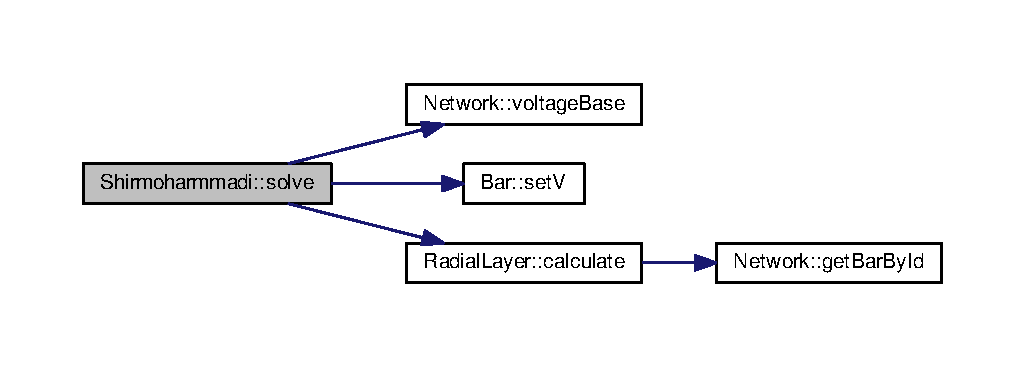
\includegraphics[width=350pt]{group___algorithms_gacb4a06c62b5d97c25bea70acd477e715_cgraph}
\end{center}
\end{figure}


\hypertarget{group___algorithms_gaee0ae606982145e66bba825421d610f8}{}\index{Algorithms@{Algorithms}!sugiyama@{sugiyama}}
\index{sugiyama@{sugiyama}!Algorithms@{Algorithms}}
\paragraph[{sugiyama}]{\setlength{\rightskip}{0pt plus 5cm}void Redraw\+Network\+::sugiyama (
\begin{DoxyParamCaption}
{}
\end{DoxyParamCaption}
)}\label{group___algorithms_gaee0ae606982145e66bba825421d610f8}
Really nice looking for radial networks. 

Definition at line \hyperlink{redrawnetwork_8cpp_source_l00106}{106} of file \hyperlink{redrawnetwork_8cpp_source}{redrawnetwork.\+cpp}.

\hypertarget{group___algorithms_ga94d53ddf8ee00c4ef6d56bb988333103}{}\index{Algorithms@{Algorithms}!sugiyama\+Fast@{sugiyama\+Fast}}
\index{sugiyama\+Fast@{sugiyama\+Fast}!Algorithms@{Algorithms}}
\paragraph[{sugiyama\+Fast}]{\setlength{\rightskip}{0pt plus 5cm}void Redraw\+Network\+::sugiyama\+Fast (
\begin{DoxyParamCaption}
{}
\end{DoxyParamCaption}
)}\label{group___algorithms_ga94d53ddf8ee00c4ef6d56bb988333103}
This will draw faster than the Sugiyama, but with a lower quality result. 

Definition at line \hyperlink{redrawnetwork_8cpp_source_l00085}{85} of file \hyperlink{redrawnetwork_8cpp_source}{redrawnetwork.\+cpp}.



Here is the caller graph for this function\+:
\nopagebreak
\begin{figure}[H]
\begin{center}
\leavevmode
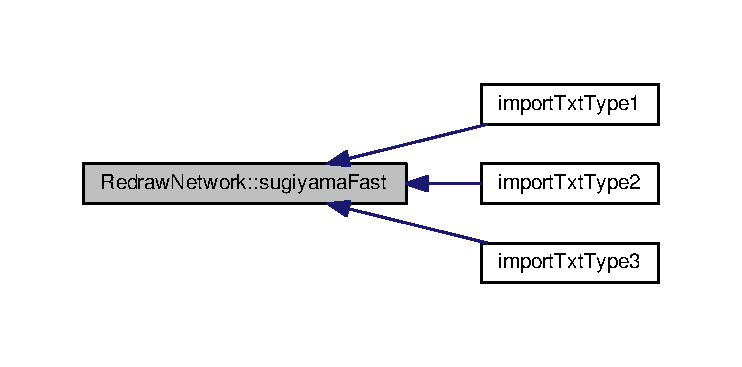
\includegraphics[width=350pt]{group___algorithms_ga94d53ddf8ee00c4ef6d56bb988333103_icgraph}
\end{center}
\end{figure}


\hypertarget{group___algorithms_gac7b5f7fdb2b88e7d8bb580834e93b1e8}{}\index{Algorithms@{Algorithms}!````~Redraw\+Network@{$\sim$\+Redraw\+Network}}
\index{````~Redraw\+Network@{$\sim$\+Redraw\+Network}!Algorithms@{Algorithms}}
\paragraph[{$\sim$\+Redraw\+Network}]{\setlength{\rightskip}{0pt plus 5cm}Redraw\+Network\+::$\sim$\+Redraw\+Network (
\begin{DoxyParamCaption}
{}
\end{DoxyParamCaption}
)}\label{group___algorithms_gac7b5f7fdb2b88e7d8bb580834e93b1e8}
Free used memory. 

Definition at line \hyperlink{redrawnetwork_8cpp_source_l00068}{68} of file \hyperlink{redrawnetwork_8cpp_source}{redrawnetwork.\+cpp}.

\hypertarget{group___algorithms_gac89016d70d3c99339af11f3b6f1f23b2}{}\index{Algorithms@{Algorithms}!````~Shirmoharmmadi@{$\sim$\+Shirmoharmmadi}}
\index{````~Shirmoharmmadi@{$\sim$\+Shirmoharmmadi}!Algorithms@{Algorithms}}
\paragraph[{$\sim$\+Shirmoharmmadi}]{\setlength{\rightskip}{0pt plus 5cm}Shirmoharmmadi\+::$\sim$\+Shirmoharmmadi (
\begin{DoxyParamCaption}
{}
\end{DoxyParamCaption}
)}\label{group___algorithms_gac89016d70d3c99339af11f3b6f1f23b2}


Definition at line \hyperlink{shirmoharmmadi_8cpp_source_l00063}{63} of file \hyperlink{shirmoharmmadi_8cpp_source}{shirmoharmmadi.\+cpp}.


\hypertarget{group___graphics}{}\subsection{Graphics}
\label{group___graphics}\index{Graphics@{Graphics}}
\subsubsection*{Files}
\begin{DoxyCompactItemize}
\item 
file \hyperlink{network_8cpp}{network.\+cpp}
\begin{DoxyCompactList}\small\item\em Implementation of \hyperlink{class_network}{Network} class. \end{DoxyCompactList}\end{DoxyCompactItemize}
\subsubsection*{Classes}
\begin{DoxyCompactItemize}
\item 
class \hyperlink{class_system_view}{System\+View}
\begin{DoxyCompactList}\small\item\em Widget to visualise Networks. \end{DoxyCompactList}\end{DoxyCompactItemize}
\subsubsection*{Functions}
\begin{DoxyCompactItemize}
\item 
\hyperlink{group___graphics_ga660a455ff7b98cb92410b0bf1cbb2eeb}{System\+View\+::\+System\+View} (Q\+Widget $\ast$parent)
\begin{DoxyCompactList}\small\item\em \hyperlink{class_system_view}{System\+View}. \end{DoxyCompactList}\item 
\hyperlink{group___graphics_ga0091352981c1efa5498819b69698db44}{System\+View\+::$\sim$\+System\+View} ()
\item 
void \hyperlink{group___graphics_ga93170319ee5fbf9098353b383fc8a368}{System\+View\+::zoom\+In} ()
\begin{DoxyCompactList}\small\item\em zoom\+In \end{DoxyCompactList}\item 
void \hyperlink{group___graphics_gaf971471c76265ec21cdde2aafe9b609f}{System\+View\+::zoom\+Out} ()
\begin{DoxyCompactList}\small\item\em zoom\+Out \end{DoxyCompactList}\item 
void \hyperlink{group___graphics_gac1bf0b6a80216df74a8da1cb8ac5f0e8}{System\+View\+::zoom\+Fit} ()
\begin{DoxyCompactList}\small\item\em zoom\+Fit \end{DoxyCompactList}\item 
void \hyperlink{group___graphics_gae183447d0777c7b2b940a977f9b64c3f}{System\+View\+::add\+Network} (\hyperlink{class_network}{Network} $\ast$network)
\begin{DoxyCompactList}\small\item\em add\+Network \end{DoxyCompactList}\item 
void \hyperlink{group___graphics_ga2078ad08ff93b9a8683d567e3f9f714e}{System\+View\+::remove\+Network} (\hyperlink{class_network}{Network} $\ast$network)
\begin{DoxyCompactList}\small\item\em remove\+Network \end{DoxyCompactList}\item 
void \hyperlink{group___graphics_gac4e02019d41c203c788ff1e6f3ee460e}{System\+View\+::add\+Bar} (\hyperlink{class_bar}{Bar} $\ast$bar)
\item 
void \hyperlink{group___graphics_ga1e96b08395a2f1b961dedbb3e8c99a50}{System\+View\+::remove\+Bar} (\hyperlink{class_bar}{Bar} $\ast$bar)
\item 
void \hyperlink{group___graphics_gaed2fb15d518cab9a52ea1ee258846bfc}{System\+View\+::add\+Line} (\hyperlink{class_line}{Line} $\ast$line)
\item 
void \hyperlink{group___graphics_ga4af1d763d9b9c02933e62d1f6231ad18}{System\+View\+::remove\+Line} (\hyperlink{class_line}{Line} $\ast$line)
\item 
void \hyperlink{group___graphics_gaab2fa6cebf9022eb6bf31497c0789675}{System\+View\+::wheel\+Event} (Q\+Wheel\+Event $\ast$event) Q\+\_\+\+D\+E\+C\+L\+\_\+\+O\+V\+E\+R\+R\+I\+D\+E
\item 
void \hyperlink{group___graphics_gab19e233cd697852dd71140971cb6e122}{System\+View\+::mouse\+Move\+Event} (Q\+Mouse\+Event $\ast$event) Q\+\_\+\+D\+E\+C\+L\+\_\+\+O\+V\+E\+R\+R\+I\+D\+E
\item 
void \hyperlink{group___graphics_ga42d4a485d6d9bd891d9505a5213cf783}{System\+View\+::mouse\+Press\+Event} (Q\+Mouse\+Event $\ast$event) Q\+\_\+\+D\+E\+C\+L\+\_\+\+O\+V\+E\+R\+R\+I\+D\+E
\item 
void \hyperlink{group___graphics_gaa8a2664405194bbe29daa454aead7416}{System\+View\+::mouse\+Release\+Event} (Q\+Mouse\+Event $\ast$event) Q\+\_\+\+D\+E\+C\+L\+\_\+\+O\+V\+E\+R\+R\+I\+D\+E
\item 
static double \hyperlink{group___graphics_ga433bc5c32cf2ce5329bb40b21952d885}{Network\+::current\+Base} ()
\item 
static double \hyperlink{group___graphics_gae6794c93d37df113778c37c2c702f6d9}{Network\+::impedance\+Base} ()
\item 
\hyperlink{group___graphics_ga3cc2fb4f8fa4d507077e8da85ce5a1c8}{Network\+::\+Network} ()
\item 
\hyperlink{group___graphics_ga7a4e19cdb4bf0c7ecf82baa643831492}{Network\+::$\sim$\+Network} ()
\item 
bool \hyperlink{group___graphics_ga8c5dfef0216731246f7411e1a5fbee01}{Network\+::add\+Bar} (\hyperlink{class_bar}{Bar} $\ast$bar)
\item 
bool \hyperlink{group___graphics_gae02945131494987b3ff9b59b627719b4}{Network\+::add\+Line} (\hyperlink{class_line}{Line} $\ast$line)
\item 
void \hyperlink{group___graphics_ga997ce4f03d316b9f138f2e64e6ca400c}{Network\+::remove\+Bar} (int32\+\_\+t id)
\item 
void \hyperlink{group___graphics_ga7dea7690987c58fa61ffaa0326b68b68}{Network\+::remove\+Bar} (\hyperlink{class_bar}{Bar} $\ast$bar)
\item 
void \hyperlink{group___graphics_ga1eef3317224a7a06348fce07e581a9ad}{Network\+::remove\+Line} (Q\+Pair$<$ int32\+\_\+t, int32\+\_\+t $>$ nodes)
\item 
void \hyperlink{group___graphics_ga4fd51288aa75614593977ce8aab9100f}{Network\+::remove\+Line} (\hyperlink{class_line}{Line} $\ast$line)
\item 
\hyperlink{class_bar}{Bar} $\ast$ \hyperlink{group___graphics_ga04d524ce0fa0dd0d06deda92b1597af0}{Network\+::get\+Bar\+By\+Id} (uint32\+\_\+t id)
\item 
\hyperlink{class_line}{Line} $\ast$ \hyperlink{group___graphics_ga8f090b85a7779695cb9f05b6395b3044}{Network\+::get\+Line\+By\+Nodes} (Q\+Pair$<$ int32\+\_\+t, int32\+\_\+t $>$ nodes)
\item 
Q\+Json\+Object \hyperlink{group___graphics_ga1bb9773d3935eefef84136d388786494}{Network\+::to\+Json} ()
\item 
void \hyperlink{group___graphics_ga2aef0f6c0d9569ec4d6b948d1ef0d5f1}{Network\+::from\+Json} (Q\+Json\+Object \&net\+Json)
\end{DoxyCompactItemize}
\subsubsection*{Variables}
\begin{DoxyCompactItemize}
\item 
static const double \hyperlink{group___graphics_gaa334bbc93b3fde219840e95e23198b53}{Network\+::bar\+Icon\+Size} = 15.\+0
\item 
static const double \hyperlink{group___graphics_ga3f810634c9908d62d33a1ab09a76c147}{Network\+::line\+Width} = 4.\+0
\item 
static const Q\+Color \hyperlink{group___graphics_gaa9e21b8e2a24b0495e776a51e1aeed94}{Network\+::selected\+Color} = Qt\+::red
\item 
static uint32\+\_\+t \hyperlink{group___graphics_ga318dee060bc577eacd67d332efbbe1b2}{Network\+::max\+Iterations} = 1000
\item 
static double \hyperlink{group___graphics_gabcdc973129d3dda7572b7a1c388da1b5}{Network\+::min\+Error} = 0.\+01
\item 
static double \hyperlink{group___graphics_ga7c1e79d9ac69df9a69f24eaf092fd5e5}{Network\+::voltage\+Base} = 23000.\+0
\item 
static double \hyperlink{group___graphics_ga74bb7aa495d422f1f092acdf958df989}{Network\+::power\+Base} = 2500000.\+0
\item 
static \hyperlink{class_unit_a8c8921f7b225ad6063b1cb573425b9a0}{Unit\+::\+Length\+Unit} \hyperlink{group___graphics_gae46c0e2bf39b343875e3c69066fe2652}{Network\+::length\+Unit} = \hyperlink{class_unit_a8c8921f7b225ad6063b1cb573425b9a0abfa41ebe7ee649a1f02c9b8ae570434b}{Unit\+::k\+Meter}
\item 
static \hyperlink{class_unit_a3747e779c805df24a71961290be3fbdf}{Unit\+::\+Impedance\+Unit} \hyperlink{group___graphics_ga5f3d72699a723c64a89d22e34df708ff}{Network\+::impedance\+Unit} = \hyperlink{class_unit_a3747e779c805df24a71961290be3fbdfa6b9c74d1763eefbaf751eeecff0bd9da}{Unit\+::k\+Ohm}
\item 
static \hyperlink{class_unit_a55b07dfa9457e1eca2c7194fe0cfc3c1}{Unit\+::\+Voltage\+Unit} \hyperlink{group___graphics_gacde031ef95f5c05565ee35769f2ed89e}{Network\+::voltage\+Unit} = \hyperlink{class_unit_a55b07dfa9457e1eca2c7194fe0cfc3c1aa54b2473993a702a3923525765bd6e4c}{Unit\+::k\+Volts}
\item 
static \hyperlink{class_unit_ace265ae255370ccacfd5370337572c3b}{Unit\+::\+Power\+Unit} \hyperlink{group___graphics_ga9504015bc566f4a3d3b4d4a86000293b}{Network\+::power\+Unit} = \hyperlink{class_unit_ace265ae255370ccacfd5370337572c3ba72b181a842ae2759488a2fa1410d3696}{Unit\+::k\+V\+A}
\item 
static \hyperlink{class_unit_a0794cf6c9682f48296dd4a5315389787}{Unit\+::\+Current\+Unit} \hyperlink{group___graphics_gac6a26db5fef2b1dd2a00faf6340d1702}{Network\+::current\+Unit} = \hyperlink{class_unit_a0794cf6c9682f48296dd4a5315389787a368a3c470f0b590a6100dda717a7dd4f}{Unit\+::k\+Ampere}
\end{DoxyCompactItemize}


\subsubsection{Detailed Description}


\subsubsection{Function Documentation}
\hypertarget{group___graphics_gac4e02019d41c203c788ff1e6f3ee460e}{}\index{Graphics@{Graphics}!add\+Bar@{add\+Bar}}
\index{add\+Bar@{add\+Bar}!Graphics@{Graphics}}
\paragraph[{add\+Bar}]{\setlength{\rightskip}{0pt plus 5cm}void System\+View\+::add\+Bar (
\begin{DoxyParamCaption}
\item[{{\bf Bar} $\ast$}]{bar}
\end{DoxyParamCaption}
)}\label{group___graphics_gac4e02019d41c203c788ff1e6f3ee460e}


Definition at line \hyperlink{systemview_8cpp_source_l00138}{138} of file \hyperlink{systemview_8cpp_source}{systemview.\+cpp}.



Here is the caller graph for this function\+:\nopagebreak
\begin{figure}[H]
\begin{center}
\leavevmode
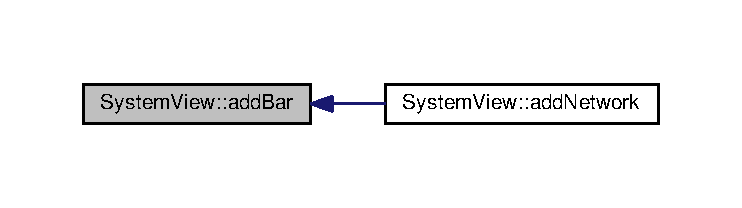
\includegraphics[width=350pt]{group___graphics_gac4e02019d41c203c788ff1e6f3ee460e_icgraph}
\end{center}
\end{figure}


\hypertarget{group___graphics_ga8c5dfef0216731246f7411e1a5fbee01}{}\index{Graphics@{Graphics}!add\+Bar@{add\+Bar}}
\index{add\+Bar@{add\+Bar}!Graphics@{Graphics}}
\paragraph[{add\+Bar}]{\setlength{\rightskip}{0pt plus 5cm}bool Network\+::add\+Bar (
\begin{DoxyParamCaption}
\item[{{\bf Bar} $\ast$}]{bar}
\end{DoxyParamCaption}
)}\label{group___graphics_ga8c5dfef0216731246f7411e1a5fbee01}


Definition at line \hyperlink{network_8cpp_source_l00118}{118} of file \hyperlink{network_8cpp_source}{network.\+cpp}.



Here is the call graph for this function\+:\nopagebreak
\begin{figure}[H]
\begin{center}
\leavevmode
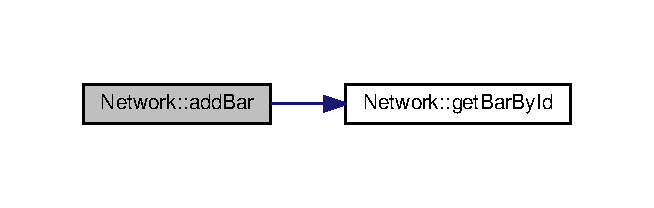
\includegraphics[width=314pt]{group___graphics_ga8c5dfef0216731246f7411e1a5fbee01_cgraph}
\end{center}
\end{figure}




Here is the caller graph for this function\+:\nopagebreak
\begin{figure}[H]
\begin{center}
\leavevmode
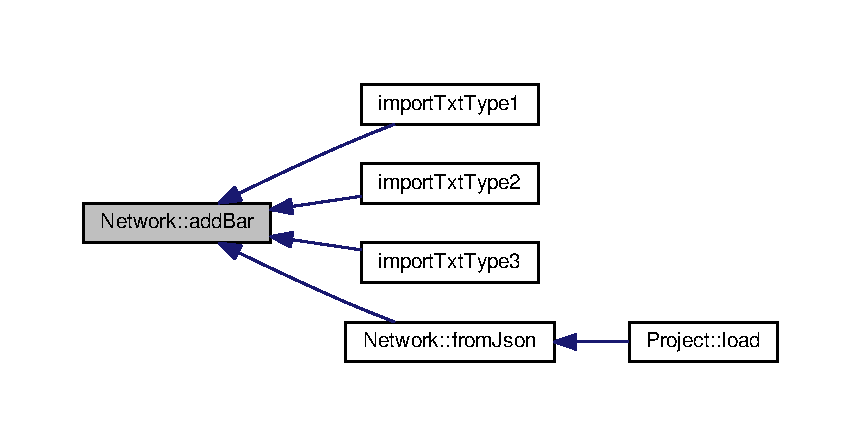
\includegraphics[width=350pt]{group___graphics_ga8c5dfef0216731246f7411e1a5fbee01_icgraph}
\end{center}
\end{figure}


\hypertarget{group___graphics_gaed2fb15d518cab9a52ea1ee258846bfc}{}\index{Graphics@{Graphics}!add\+Line@{add\+Line}}
\index{add\+Line@{add\+Line}!Graphics@{Graphics}}
\paragraph[{add\+Line}]{\setlength{\rightskip}{0pt plus 5cm}void System\+View\+::add\+Line (
\begin{DoxyParamCaption}
\item[{{\bf Line} $\ast$}]{line}
\end{DoxyParamCaption}
)}\label{group___graphics_gaed2fb15d518cab9a52ea1ee258846bfc}


Definition at line \hyperlink{systemview_8cpp_source_l00155}{155} of file \hyperlink{systemview_8cpp_source}{systemview.\+cpp}.



Here is the caller graph for this function\+:\nopagebreak
\begin{figure}[H]
\begin{center}
\leavevmode
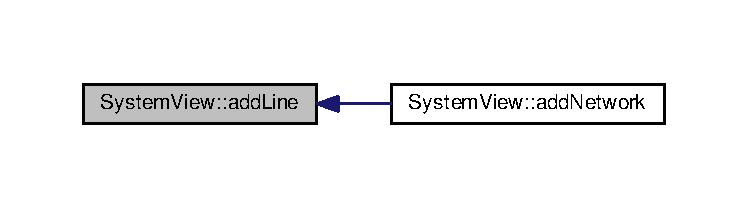
\includegraphics[width=350pt]{group___graphics_gaed2fb15d518cab9a52ea1ee258846bfc_icgraph}
\end{center}
\end{figure}


\hypertarget{group___graphics_gae02945131494987b3ff9b59b627719b4}{}\index{Graphics@{Graphics}!add\+Line@{add\+Line}}
\index{add\+Line@{add\+Line}!Graphics@{Graphics}}
\paragraph[{add\+Line}]{\setlength{\rightskip}{0pt plus 5cm}bool Network\+::add\+Line (
\begin{DoxyParamCaption}
\item[{{\bf Line} $\ast$}]{line}
\end{DoxyParamCaption}
)}\label{group___graphics_gae02945131494987b3ff9b59b627719b4}


Definition at line \hyperlink{network_8cpp_source_l00133}{133} of file \hyperlink{network_8cpp_source}{network.\+cpp}.



Here is the call graph for this function\+:\nopagebreak
\begin{figure}[H]
\begin{center}
\leavevmode
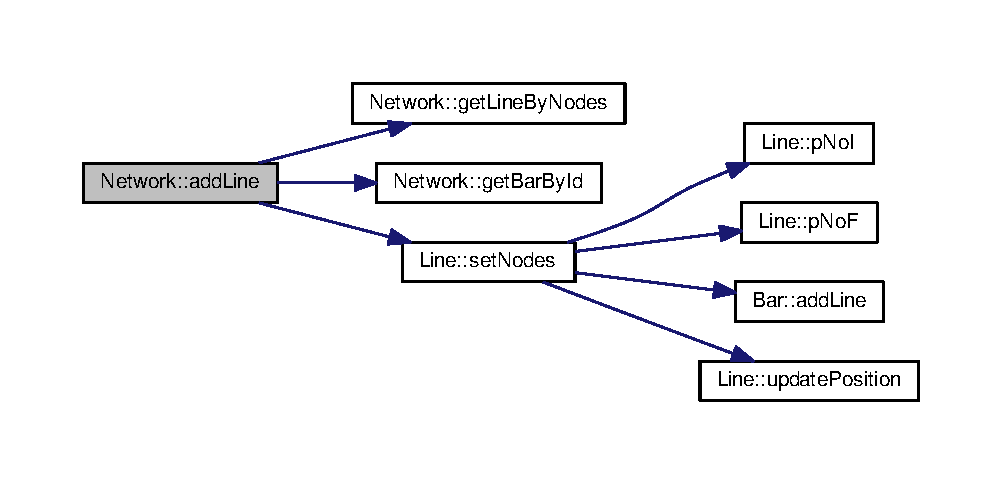
\includegraphics[width=350pt]{group___graphics_gae02945131494987b3ff9b59b627719b4_cgraph}
\end{center}
\end{figure}




Here is the caller graph for this function\+:\nopagebreak
\begin{figure}[H]
\begin{center}
\leavevmode
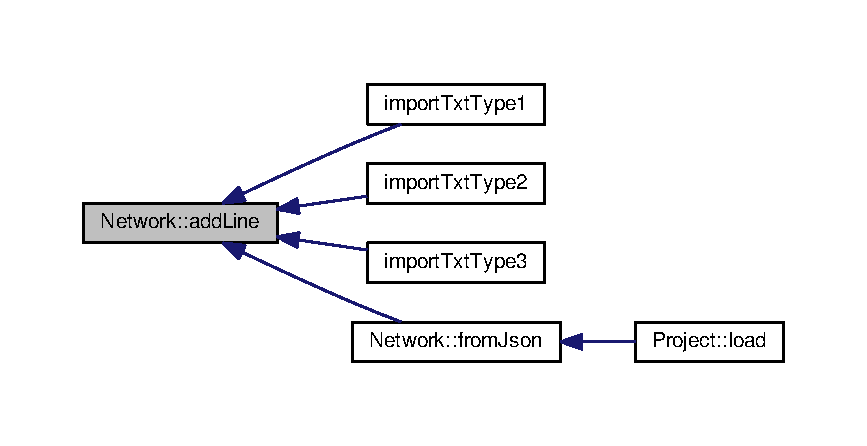
\includegraphics[width=350pt]{group___graphics_gae02945131494987b3ff9b59b627719b4_icgraph}
\end{center}
\end{figure}


\hypertarget{group___graphics_gae183447d0777c7b2b940a977f9b64c3f}{}\index{Graphics@{Graphics}!add\+Network@{add\+Network}}
\index{add\+Network@{add\+Network}!Graphics@{Graphics}}
\paragraph[{add\+Network}]{\setlength{\rightskip}{0pt plus 5cm}void System\+View\+::add\+Network (
\begin{DoxyParamCaption}
\item[{{\bf Network} $\ast$}]{network}
\end{DoxyParamCaption}
)}\label{group___graphics_gae183447d0777c7b2b940a977f9b64c3f}

\begin{DoxyParams}{Parameters}
{\em network} & \\
\hline
\end{DoxyParams}


Definition at line \hyperlink{systemview_8cpp_source_l00112}{112} of file \hyperlink{systemview_8cpp_source}{systemview.\+cpp}.



Here is the call graph for this function\+:\nopagebreak
\begin{figure}[H]
\begin{center}
\leavevmode
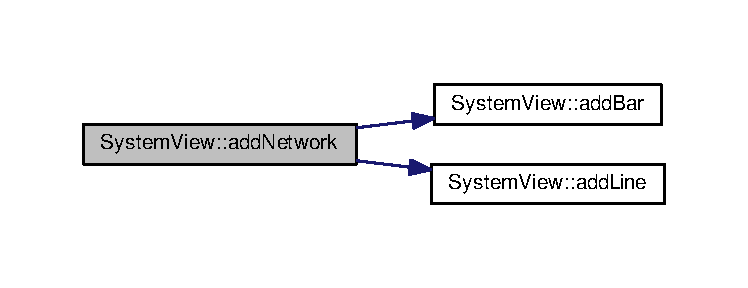
\includegraphics[width=350pt]{group___graphics_gae183447d0777c7b2b940a977f9b64c3f_cgraph}
\end{center}
\end{figure}


\hypertarget{group___graphics_ga433bc5c32cf2ce5329bb40b21952d885}{}\index{Graphics@{Graphics}!current\+Base@{current\+Base}}
\index{current\+Base@{current\+Base}!Graphics@{Graphics}}
\paragraph[{current\+Base}]{\setlength{\rightskip}{0pt plus 5cm}double Network\+::current\+Base (
\begin{DoxyParamCaption}
{}
\end{DoxyParamCaption}
)\hspace{0.3cm}{\ttfamily [static]}}\label{group___graphics_ga433bc5c32cf2ce5329bb40b21952d885}


Definition at line \hyperlink{network_8cpp_source_l00077}{77} of file \hyperlink{network_8cpp_source}{network.\+cpp}.



Here is the caller graph for this function\+:\nopagebreak
\begin{figure}[H]
\begin{center}
\leavevmode
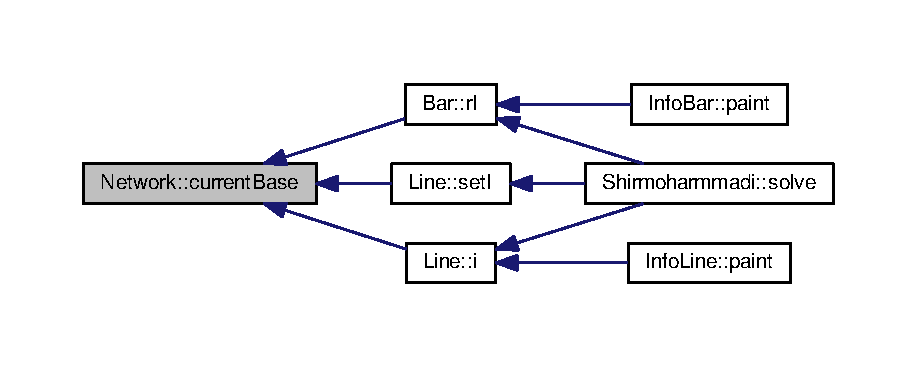
\includegraphics[width=350pt]{group___graphics_ga433bc5c32cf2ce5329bb40b21952d885_icgraph}
\end{center}
\end{figure}


\hypertarget{group___graphics_ga2aef0f6c0d9569ec4d6b948d1ef0d5f1}{}\index{Graphics@{Graphics}!from\+Json@{from\+Json}}
\index{from\+Json@{from\+Json}!Graphics@{Graphics}}
\paragraph[{from\+Json}]{\setlength{\rightskip}{0pt plus 5cm}void Network\+::from\+Json (
\begin{DoxyParamCaption}
\item[{Q\+Json\+Object \&}]{net\+Json}
\end{DoxyParamCaption}
)}\label{group___graphics_ga2aef0f6c0d9569ec4d6b948d1ef0d5f1}


Definition at line \hyperlink{network_8cpp_source_l00236}{236} of file \hyperlink{network_8cpp_source}{network.\+cpp}.



Here is the call graph for this function\+:\nopagebreak
\begin{figure}[H]
\begin{center}
\leavevmode
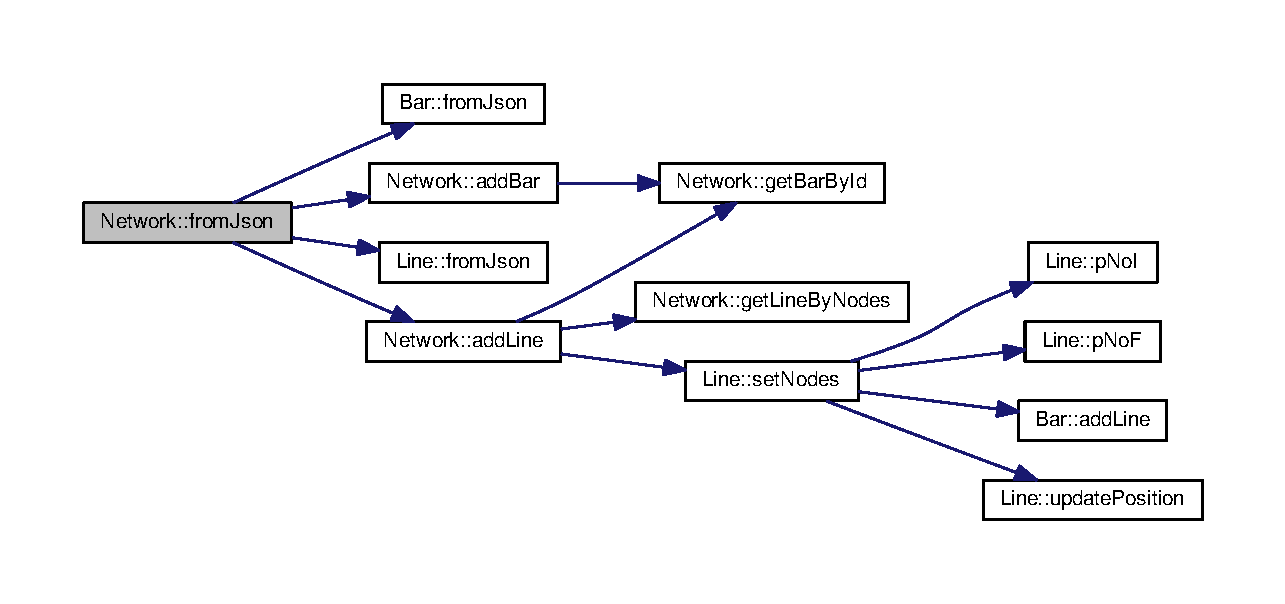
\includegraphics[width=350pt]{group___graphics_ga2aef0f6c0d9569ec4d6b948d1ef0d5f1_cgraph}
\end{center}
\end{figure}




Here is the caller graph for this function\+:\nopagebreak
\begin{figure}[H]
\begin{center}
\leavevmode
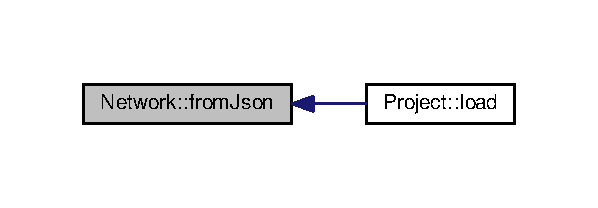
\includegraphics[width=287pt]{group___graphics_ga2aef0f6c0d9569ec4d6b948d1ef0d5f1_icgraph}
\end{center}
\end{figure}


\hypertarget{group___graphics_ga04d524ce0fa0dd0d06deda92b1597af0}{}\index{Graphics@{Graphics}!get\+Bar\+By\+Id@{get\+Bar\+By\+Id}}
\index{get\+Bar\+By\+Id@{get\+Bar\+By\+Id}!Graphics@{Graphics}}
\paragraph[{get\+Bar\+By\+Id}]{\setlength{\rightskip}{0pt plus 5cm}{\bf Bar} $\ast$ Network\+::get\+Bar\+By\+Id (
\begin{DoxyParamCaption}
\item[{uint32\+\_\+t}]{id}
\end{DoxyParamCaption}
)}\label{group___graphics_ga04d524ce0fa0dd0d06deda92b1597af0}


Definition at line \hyperlink{network_8cpp_source_l00190}{190} of file \hyperlink{network_8cpp_source}{network.\+cpp}.



Here is the caller graph for this function\+:\nopagebreak
\begin{figure}[H]
\begin{center}
\leavevmode
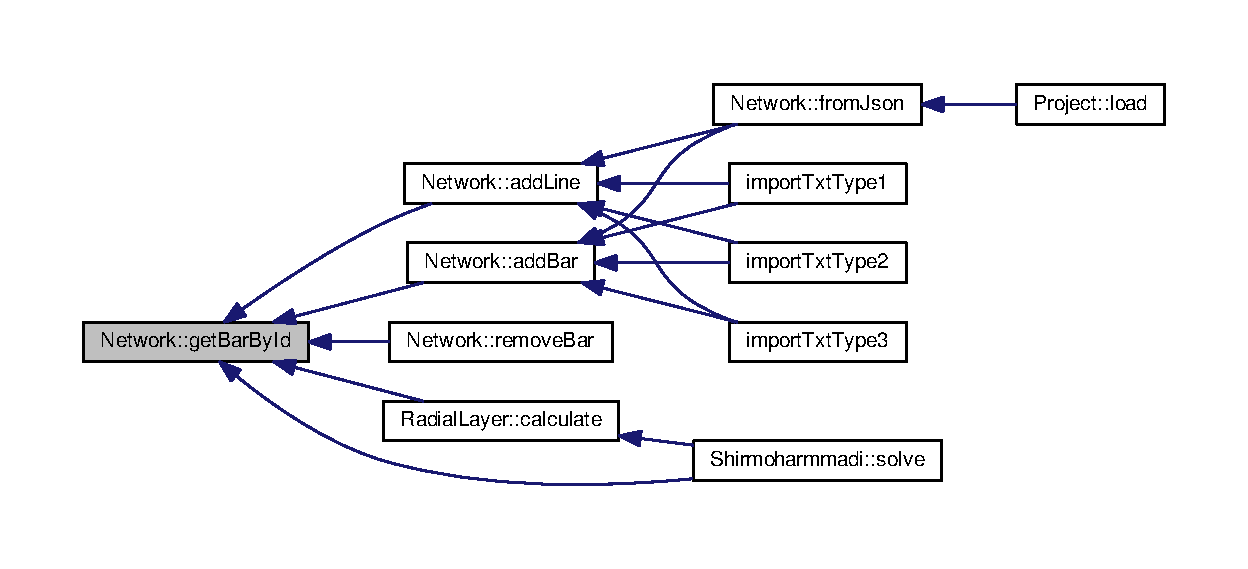
\includegraphics[width=350pt]{group___graphics_ga04d524ce0fa0dd0d06deda92b1597af0_icgraph}
\end{center}
\end{figure}


\hypertarget{group___graphics_ga8f090b85a7779695cb9f05b6395b3044}{}\index{Graphics@{Graphics}!get\+Line\+By\+Nodes@{get\+Line\+By\+Nodes}}
\index{get\+Line\+By\+Nodes@{get\+Line\+By\+Nodes}!Graphics@{Graphics}}
\paragraph[{get\+Line\+By\+Nodes}]{\setlength{\rightskip}{0pt plus 5cm}{\bf Line} $\ast$ Network\+::get\+Line\+By\+Nodes (
\begin{DoxyParamCaption}
\item[{Q\+Pair$<$ int32\+\_\+t, int32\+\_\+t $>$}]{nodes}
\end{DoxyParamCaption}
)}\label{group___graphics_ga8f090b85a7779695cb9f05b6395b3044}


Definition at line \hyperlink{network_8cpp_source_l00198}{198} of file \hyperlink{network_8cpp_source}{network.\+cpp}.



Here is the caller graph for this function\+:\nopagebreak
\begin{figure}[H]
\begin{center}
\leavevmode
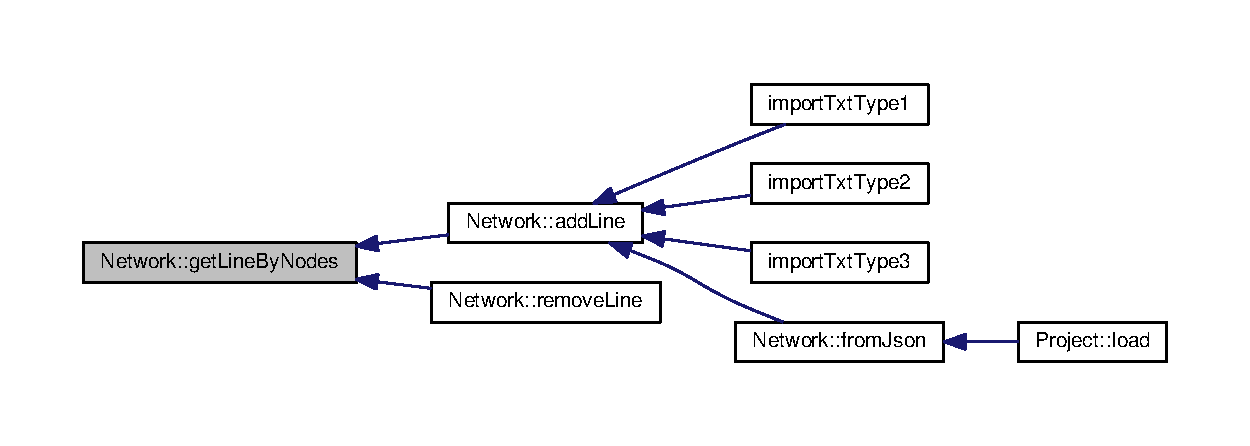
\includegraphics[width=350pt]{group___graphics_ga8f090b85a7779695cb9f05b6395b3044_icgraph}
\end{center}
\end{figure}


\hypertarget{group___graphics_gae6794c93d37df113778c37c2c702f6d9}{}\index{Graphics@{Graphics}!impedance\+Base@{impedance\+Base}}
\index{impedance\+Base@{impedance\+Base}!Graphics@{Graphics}}
\paragraph[{impedance\+Base}]{\setlength{\rightskip}{0pt plus 5cm}double Network\+::impedance\+Base (
\begin{DoxyParamCaption}
{}
\end{DoxyParamCaption}
)\hspace{0.3cm}{\ttfamily [static]}}\label{group___graphics_gae6794c93d37df113778c37c2c702f6d9}


Definition at line \hyperlink{network_8cpp_source_l00085}{85} of file \hyperlink{network_8cpp_source}{network.\+cpp}.



Here is the caller graph for this function\+:\nopagebreak
\begin{figure}[H]
\begin{center}
\leavevmode
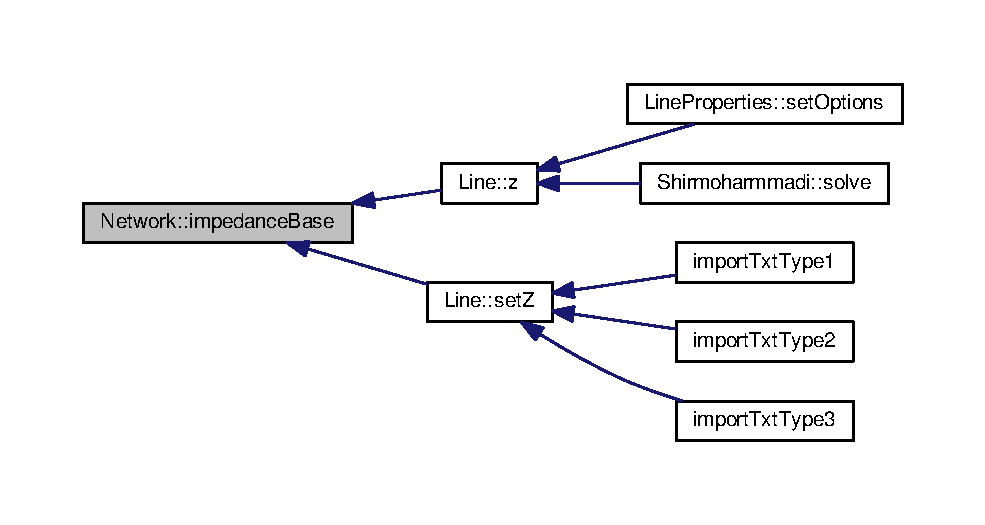
\includegraphics[width=350pt]{group___graphics_gae6794c93d37df113778c37c2c702f6d9_icgraph}
\end{center}
\end{figure}


\hypertarget{group___graphics_gab19e233cd697852dd71140971cb6e122}{}\index{Graphics@{Graphics}!mouse\+Move\+Event@{mouse\+Move\+Event}}
\index{mouse\+Move\+Event@{mouse\+Move\+Event}!Graphics@{Graphics}}
\paragraph[{mouse\+Move\+Event}]{\setlength{\rightskip}{0pt plus 5cm}void System\+View\+::mouse\+Move\+Event (
\begin{DoxyParamCaption}
\item[{Q\+Mouse\+Event $\ast$}]{event}
\end{DoxyParamCaption}
)\hspace{0.3cm}{\ttfamily [protected]}}\label{group___graphics_gab19e233cd697852dd71140971cb6e122}


Definition at line \hyperlink{systemview_8cpp_source_l00188}{188} of file \hyperlink{systemview_8cpp_source}{systemview.\+cpp}.

\hypertarget{group___graphics_ga42d4a485d6d9bd891d9505a5213cf783}{}\index{Graphics@{Graphics}!mouse\+Press\+Event@{mouse\+Press\+Event}}
\index{mouse\+Press\+Event@{mouse\+Press\+Event}!Graphics@{Graphics}}
\paragraph[{mouse\+Press\+Event}]{\setlength{\rightskip}{0pt plus 5cm}void System\+View\+::mouse\+Press\+Event (
\begin{DoxyParamCaption}
\item[{Q\+Mouse\+Event $\ast$}]{event}
\end{DoxyParamCaption}
)\hspace{0.3cm}{\ttfamily [protected]}}\label{group___graphics_ga42d4a485d6d9bd891d9505a5213cf783}


Definition at line \hyperlink{systemview_8cpp_source_l00205}{205} of file \hyperlink{systemview_8cpp_source}{systemview.\+cpp}.

\hypertarget{group___graphics_gaa8a2664405194bbe29daa454aead7416}{}\index{Graphics@{Graphics}!mouse\+Release\+Event@{mouse\+Release\+Event}}
\index{mouse\+Release\+Event@{mouse\+Release\+Event}!Graphics@{Graphics}}
\paragraph[{mouse\+Release\+Event}]{\setlength{\rightskip}{0pt plus 5cm}void System\+View\+::mouse\+Release\+Event (
\begin{DoxyParamCaption}
\item[{Q\+Mouse\+Event $\ast$}]{event}
\end{DoxyParamCaption}
)\hspace{0.3cm}{\ttfamily [protected]}}\label{group___graphics_gaa8a2664405194bbe29daa454aead7416}


Definition at line \hyperlink{systemview_8cpp_source_l00219}{219} of file \hyperlink{systemview_8cpp_source}{systemview.\+cpp}.

\hypertarget{group___graphics_ga3cc2fb4f8fa4d507077e8da85ce5a1c8}{}\index{Graphics@{Graphics}!Network@{Network}}
\index{Network@{Network}!Graphics@{Graphics}}
\paragraph[{Network}]{\setlength{\rightskip}{0pt plus 5cm}Network\+::\+Network (
\begin{DoxyParamCaption}
{}
\end{DoxyParamCaption}
)}\label{group___graphics_ga3cc2fb4f8fa4d507077e8da85ce5a1c8}


Definition at line \hyperlink{network_8cpp_source_l00093}{93} of file \hyperlink{network_8cpp_source}{network.\+cpp}.

\hypertarget{group___graphics_ga1e96b08395a2f1b961dedbb3e8c99a50}{}\index{Graphics@{Graphics}!remove\+Bar@{remove\+Bar}}
\index{remove\+Bar@{remove\+Bar}!Graphics@{Graphics}}
\paragraph[{remove\+Bar}]{\setlength{\rightskip}{0pt plus 5cm}void System\+View\+::remove\+Bar (
\begin{DoxyParamCaption}
\item[{{\bf Bar} $\ast$}]{bar}
\end{DoxyParamCaption}
)}\label{group___graphics_ga1e96b08395a2f1b961dedbb3e8c99a50}


Definition at line \hyperlink{systemview_8cpp_source_l00147}{147} of file \hyperlink{systemview_8cpp_source}{systemview.\+cpp}.



Here is the caller graph for this function\+:\nopagebreak
\begin{figure}[H]
\begin{center}
\leavevmode
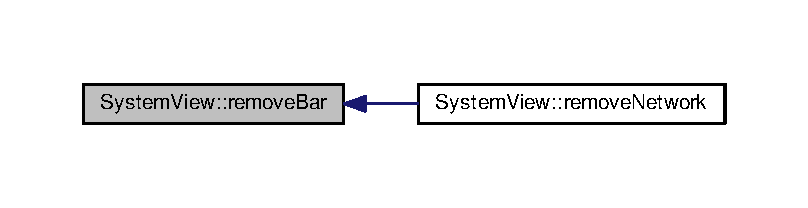
\includegraphics[width=350pt]{group___graphics_ga1e96b08395a2f1b961dedbb3e8c99a50_icgraph}
\end{center}
\end{figure}


\hypertarget{group___graphics_ga997ce4f03d316b9f138f2e64e6ca400c}{}\index{Graphics@{Graphics}!remove\+Bar@{remove\+Bar}}
\index{remove\+Bar@{remove\+Bar}!Graphics@{Graphics}}
\paragraph[{remove\+Bar}]{\setlength{\rightskip}{0pt plus 5cm}void Network\+::remove\+Bar (
\begin{DoxyParamCaption}
\item[{int32\+\_\+t}]{id}
\end{DoxyParamCaption}
)}\label{group___graphics_ga997ce4f03d316b9f138f2e64e6ca400c}


Definition at line \hyperlink{network_8cpp_source_l00158}{158} of file \hyperlink{network_8cpp_source}{network.\+cpp}.



Here is the call graph for this function\+:\nopagebreak
\begin{figure}[H]
\begin{center}
\leavevmode
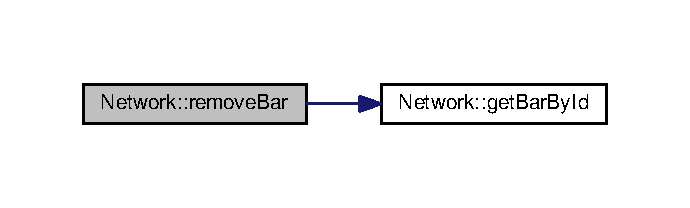
\includegraphics[width=331pt]{group___graphics_ga997ce4f03d316b9f138f2e64e6ca400c_cgraph}
\end{center}
\end{figure}


\hypertarget{group___graphics_ga7dea7690987c58fa61ffaa0326b68b68}{}\index{Graphics@{Graphics}!remove\+Bar@{remove\+Bar}}
\index{remove\+Bar@{remove\+Bar}!Graphics@{Graphics}}
\paragraph[{remove\+Bar}]{\setlength{\rightskip}{0pt plus 5cm}void Network\+::remove\+Bar (
\begin{DoxyParamCaption}
\item[{{\bf Bar} $\ast$}]{bar}
\end{DoxyParamCaption}
)}\label{group___graphics_ga7dea7690987c58fa61ffaa0326b68b68}


Definition at line \hyperlink{network_8cpp_source_l00166}{166} of file \hyperlink{network_8cpp_source}{network.\+cpp}.

\hypertarget{group___graphics_ga4af1d763d9b9c02933e62d1f6231ad18}{}\index{Graphics@{Graphics}!remove\+Line@{remove\+Line}}
\index{remove\+Line@{remove\+Line}!Graphics@{Graphics}}
\paragraph[{remove\+Line}]{\setlength{\rightskip}{0pt plus 5cm}void System\+View\+::remove\+Line (
\begin{DoxyParamCaption}
\item[{{\bf Line} $\ast$}]{line}
\end{DoxyParamCaption}
)}\label{group___graphics_ga4af1d763d9b9c02933e62d1f6231ad18}


Definition at line \hyperlink{systemview_8cpp_source_l00164}{164} of file \hyperlink{systemview_8cpp_source}{systemview.\+cpp}.



Here is the caller graph for this function\+:\nopagebreak
\begin{figure}[H]
\begin{center}
\leavevmode
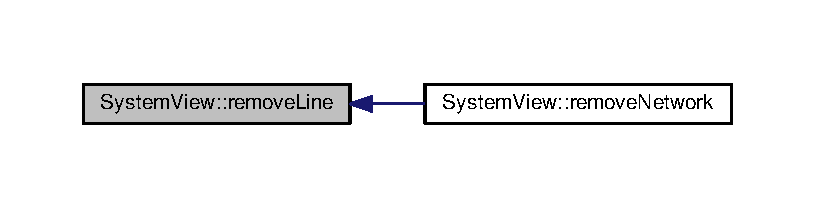
\includegraphics[width=350pt]{group___graphics_ga4af1d763d9b9c02933e62d1f6231ad18_icgraph}
\end{center}
\end{figure}


\hypertarget{group___graphics_ga1eef3317224a7a06348fce07e581a9ad}{}\index{Graphics@{Graphics}!remove\+Line@{remove\+Line}}
\index{remove\+Line@{remove\+Line}!Graphics@{Graphics}}
\paragraph[{remove\+Line}]{\setlength{\rightskip}{0pt plus 5cm}void Network\+::remove\+Line (
\begin{DoxyParamCaption}
\item[{Q\+Pair$<$ int32\+\_\+t, int32\+\_\+t $>$}]{nodes}
\end{DoxyParamCaption}
)}\label{group___graphics_ga1eef3317224a7a06348fce07e581a9ad}


Definition at line \hyperlink{network_8cpp_source_l00174}{174} of file \hyperlink{network_8cpp_source}{network.\+cpp}.



Here is the call graph for this function\+:\nopagebreak
\begin{figure}[H]
\begin{center}
\leavevmode
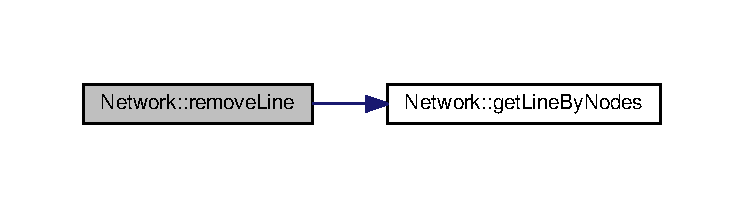
\includegraphics[width=350pt]{group___graphics_ga1eef3317224a7a06348fce07e581a9ad_cgraph}
\end{center}
\end{figure}


\hypertarget{group___graphics_ga4fd51288aa75614593977ce8aab9100f}{}\index{Graphics@{Graphics}!remove\+Line@{remove\+Line}}
\index{remove\+Line@{remove\+Line}!Graphics@{Graphics}}
\paragraph[{remove\+Line}]{\setlength{\rightskip}{0pt plus 5cm}void Network\+::remove\+Line (
\begin{DoxyParamCaption}
\item[{{\bf Line} $\ast$}]{line}
\end{DoxyParamCaption}
)}\label{group___graphics_ga4fd51288aa75614593977ce8aab9100f}


Definition at line \hyperlink{network_8cpp_source_l00182}{182} of file \hyperlink{network_8cpp_source}{network.\+cpp}.

\hypertarget{group___graphics_ga2078ad08ff93b9a8683d567e3f9f714e}{}\index{Graphics@{Graphics}!remove\+Network@{remove\+Network}}
\index{remove\+Network@{remove\+Network}!Graphics@{Graphics}}
\paragraph[{remove\+Network}]{\setlength{\rightskip}{0pt plus 5cm}void System\+View\+::remove\+Network (
\begin{DoxyParamCaption}
\item[{{\bf Network} $\ast$}]{network}
\end{DoxyParamCaption}
)}\label{group___graphics_ga2078ad08ff93b9a8683d567e3f9f714e}

\begin{DoxyParams}{Parameters}
{\em network} & \\
\hline
\end{DoxyParams}


Definition at line \hyperlink{systemview_8cpp_source_l00126}{126} of file \hyperlink{systemview_8cpp_source}{systemview.\+cpp}.



Here is the call graph for this function\+:\nopagebreak
\begin{figure}[H]
\begin{center}
\leavevmode
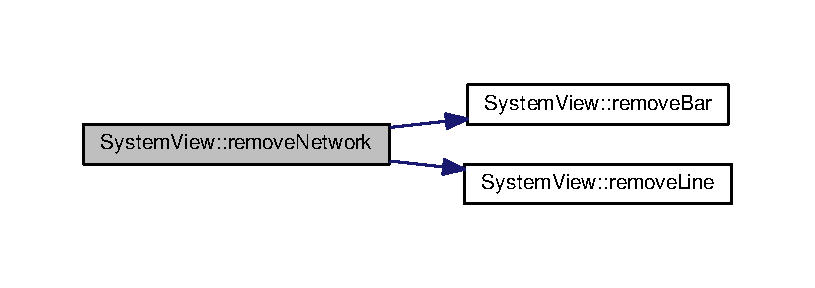
\includegraphics[width=350pt]{group___graphics_ga2078ad08ff93b9a8683d567e3f9f714e_cgraph}
\end{center}
\end{figure}


\hypertarget{group___graphics_ga660a455ff7b98cb92410b0bf1cbb2eeb}{}\index{Graphics@{Graphics}!System\+View@{System\+View}}
\index{System\+View@{System\+View}!Graphics@{Graphics}}
\paragraph[{System\+View}]{\setlength{\rightskip}{0pt plus 5cm}System\+View\+::\+System\+View (
\begin{DoxyParamCaption}
\item[{Q\+Widget $\ast$}]{parent}
\end{DoxyParamCaption}
)}\label{group___graphics_ga660a455ff7b98cb92410b0bf1cbb2eeb}

\begin{DoxyParams}{Parameters}
{\em parent} & \\
\hline
\end{DoxyParams}


Definition at line \hyperlink{systemview_8cpp_source_l00055}{55} of file \hyperlink{systemview_8cpp_source}{systemview.\+cpp}.

\hypertarget{group___graphics_ga1bb9773d3935eefef84136d388786494}{}\index{Graphics@{Graphics}!to\+Json@{to\+Json}}
\index{to\+Json@{to\+Json}!Graphics@{Graphics}}
\paragraph[{to\+Json}]{\setlength{\rightskip}{0pt plus 5cm}Q\+Json\+Object Network\+::to\+Json (
\begin{DoxyParamCaption}
{}
\end{DoxyParamCaption}
)}\label{group___graphics_ga1bb9773d3935eefef84136d388786494}


Definition at line \hyperlink{network_8cpp_source_l00206}{206} of file \hyperlink{network_8cpp_source}{network.\+cpp}.



Here is the call graph for this function\+:\nopagebreak
\begin{figure}[H]
\begin{center}
\leavevmode
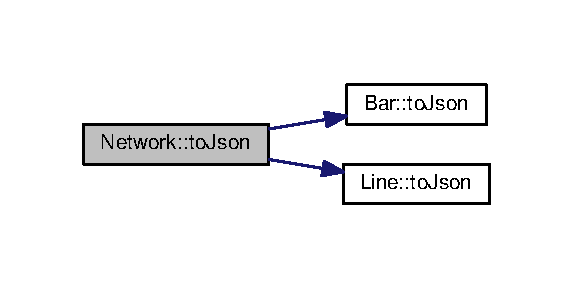
\includegraphics[width=275pt]{group___graphics_ga1bb9773d3935eefef84136d388786494_cgraph}
\end{center}
\end{figure}




Here is the caller graph for this function\+:\nopagebreak
\begin{figure}[H]
\begin{center}
\leavevmode
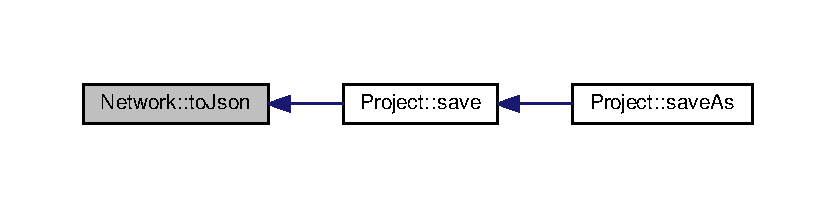
\includegraphics[width=350pt]{group___graphics_ga1bb9773d3935eefef84136d388786494_icgraph}
\end{center}
\end{figure}


\hypertarget{group___graphics_gaab2fa6cebf9022eb6bf31497c0789675}{}\index{Graphics@{Graphics}!wheel\+Event@{wheel\+Event}}
\index{wheel\+Event@{wheel\+Event}!Graphics@{Graphics}}
\paragraph[{wheel\+Event}]{\setlength{\rightskip}{0pt plus 5cm}void System\+View\+::wheel\+Event (
\begin{DoxyParamCaption}
\item[{Q\+Wheel\+Event $\ast$}]{event}
\end{DoxyParamCaption}
)\hspace{0.3cm}{\ttfamily [protected]}}\label{group___graphics_gaab2fa6cebf9022eb6bf31497c0789675}


Definition at line \hyperlink{systemview_8cpp_source_l00174}{174} of file \hyperlink{systemview_8cpp_source}{systemview.\+cpp}.

\hypertarget{group___graphics_gac1bf0b6a80216df74a8da1cb8ac5f0e8}{}\index{Graphics@{Graphics}!zoom\+Fit@{zoom\+Fit}}
\index{zoom\+Fit@{zoom\+Fit}!Graphics@{Graphics}}
\paragraph[{zoom\+Fit}]{\setlength{\rightskip}{0pt plus 5cm}void System\+View\+::zoom\+Fit (
\begin{DoxyParamCaption}
{}
\end{DoxyParamCaption}
)}\label{group___graphics_gac1bf0b6a80216df74a8da1cb8ac5f0e8}


Definition at line \hyperlink{systemview_8cpp_source_l00104}{104} of file \hyperlink{systemview_8cpp_source}{systemview.\+cpp}.

\hypertarget{group___graphics_ga93170319ee5fbf9098353b383fc8a368}{}\index{Graphics@{Graphics}!zoom\+In@{zoom\+In}}
\index{zoom\+In@{zoom\+In}!Graphics@{Graphics}}
\paragraph[{zoom\+In}]{\setlength{\rightskip}{0pt plus 5cm}void System\+View\+::zoom\+In (
\begin{DoxyParamCaption}
{}
\end{DoxyParamCaption}
)}\label{group___graphics_ga93170319ee5fbf9098353b383fc8a368}


Definition at line \hyperlink{systemview_8cpp_source_l00088}{88} of file \hyperlink{systemview_8cpp_source}{systemview.\+cpp}.

\hypertarget{group___graphics_gaf971471c76265ec21cdde2aafe9b609f}{}\index{Graphics@{Graphics}!zoom\+Out@{zoom\+Out}}
\index{zoom\+Out@{zoom\+Out}!Graphics@{Graphics}}
\paragraph[{zoom\+Out}]{\setlength{\rightskip}{0pt plus 5cm}void System\+View\+::zoom\+Out (
\begin{DoxyParamCaption}
{}
\end{DoxyParamCaption}
)}\label{group___graphics_gaf971471c76265ec21cdde2aafe9b609f}


Definition at line \hyperlink{systemview_8cpp_source_l00096}{96} of file \hyperlink{systemview_8cpp_source}{systemview.\+cpp}.

\hypertarget{group___graphics_ga7a4e19cdb4bf0c7ecf82baa643831492}{}\index{Graphics@{Graphics}!````~Network@{$\sim$\+Network}}
\index{````~Network@{$\sim$\+Network}!Graphics@{Graphics}}
\paragraph[{$\sim$\+Network}]{\setlength{\rightskip}{0pt plus 5cm}Network\+::$\sim$\+Network (
\begin{DoxyParamCaption}
{}
\end{DoxyParamCaption}
)}\label{group___graphics_ga7a4e19cdb4bf0c7ecf82baa643831492}


Definition at line \hyperlink{network_8cpp_source_l00104}{104} of file \hyperlink{network_8cpp_source}{network.\+cpp}.

\hypertarget{group___graphics_ga0091352981c1efa5498819b69698db44}{}\index{Graphics@{Graphics}!````~System\+View@{$\sim$\+System\+View}}
\index{````~System\+View@{$\sim$\+System\+View}!Graphics@{Graphics}}
\paragraph[{$\sim$\+System\+View}]{\setlength{\rightskip}{0pt plus 5cm}System\+View\+::$\sim$\+System\+View (
\begin{DoxyParamCaption}
{}
\end{DoxyParamCaption}
)}\label{group___graphics_ga0091352981c1efa5498819b69698db44}


Definition at line \hyperlink{systemview_8cpp_source_l00080}{80} of file \hyperlink{systemview_8cpp_source}{systemview.\+cpp}.



\subsubsection{Variable Documentation}
\hypertarget{group___graphics_gaa334bbc93b3fde219840e95e23198b53}{}\index{Graphics@{Graphics}!bar\+Icon\+Size@{bar\+Icon\+Size}}
\index{bar\+Icon\+Size@{bar\+Icon\+Size}!Graphics@{Graphics}}
\paragraph[{bar\+Icon\+Size}]{\setlength{\rightskip}{0pt plus 5cm}const double Network\+::bar\+Icon\+Size = 15.\+0\hspace{0.3cm}{\ttfamily [static]}}\label{group___graphics_gaa334bbc93b3fde219840e95e23198b53}


Definition at line \hyperlink{network_8h_source_l00084}{84} of file \hyperlink{network_8h_source}{network.\+h}.

\hypertarget{group___graphics_gac6a26db5fef2b1dd2a00faf6340d1702}{}\index{Graphics@{Graphics}!current\+Unit@{current\+Unit}}
\index{current\+Unit@{current\+Unit}!Graphics@{Graphics}}
\paragraph[{current\+Unit}]{\setlength{\rightskip}{0pt plus 5cm}{\bf Unit\+::\+Current\+Unit} Network\+::current\+Unit = {\bf Unit\+::k\+Ampere}\hspace{0.3cm}{\ttfamily [static]}}\label{group___graphics_gac6a26db5fef2b1dd2a00faf6340d1702}


Definition at line \hyperlink{network_8h_source_l00109}{109} of file \hyperlink{network_8h_source}{network.\+h}.

\hypertarget{group___graphics_ga5f3d72699a723c64a89d22e34df708ff}{}\index{Graphics@{Graphics}!impedance\+Unit@{impedance\+Unit}}
\index{impedance\+Unit@{impedance\+Unit}!Graphics@{Graphics}}
\paragraph[{impedance\+Unit}]{\setlength{\rightskip}{0pt plus 5cm}{\bf Unit\+::\+Impedance\+Unit} Network\+::impedance\+Unit = {\bf Unit\+::k\+Ohm}\hspace{0.3cm}{\ttfamily [static]}}\label{group___graphics_ga5f3d72699a723c64a89d22e34df708ff}


Definition at line \hyperlink{network_8h_source_l00103}{103} of file \hyperlink{network_8h_source}{network.\+h}.

\hypertarget{group___graphics_gae46c0e2bf39b343875e3c69066fe2652}{}\index{Graphics@{Graphics}!length\+Unit@{length\+Unit}}
\index{length\+Unit@{length\+Unit}!Graphics@{Graphics}}
\paragraph[{length\+Unit}]{\setlength{\rightskip}{0pt plus 5cm}{\bf Unit\+::\+Length\+Unit} Network\+::length\+Unit = {\bf Unit\+::k\+Meter}\hspace{0.3cm}{\ttfamily [static]}}\label{group___graphics_gae46c0e2bf39b343875e3c69066fe2652}


Definition at line \hyperlink{network_8h_source_l00101}{101} of file \hyperlink{network_8h_source}{network.\+h}.

\hypertarget{group___graphics_ga3f810634c9908d62d33a1ab09a76c147}{}\index{Graphics@{Graphics}!line\+Width@{line\+Width}}
\index{line\+Width@{line\+Width}!Graphics@{Graphics}}
\paragraph[{line\+Width}]{\setlength{\rightskip}{0pt plus 5cm}const double Network\+::line\+Width = 4.\+0\hspace{0.3cm}{\ttfamily [static]}}\label{group___graphics_ga3f810634c9908d62d33a1ab09a76c147}


Definition at line \hyperlink{network_8h_source_l00086}{86} of file \hyperlink{network_8h_source}{network.\+h}.

\hypertarget{group___graphics_ga318dee060bc577eacd67d332efbbe1b2}{}\index{Graphics@{Graphics}!max\+Iterations@{max\+Iterations}}
\index{max\+Iterations@{max\+Iterations}!Graphics@{Graphics}}
\paragraph[{max\+Iterations}]{\setlength{\rightskip}{0pt plus 5cm}uint32\+\_\+t Network\+::max\+Iterations = 1000\hspace{0.3cm}{\ttfamily [static]}}\label{group___graphics_ga318dee060bc577eacd67d332efbbe1b2}


Definition at line \hyperlink{network_8h_source_l00093}{93} of file \hyperlink{network_8h_source}{network.\+h}.

\hypertarget{group___graphics_gabcdc973129d3dda7572b7a1c388da1b5}{}\index{Graphics@{Graphics}!min\+Error@{min\+Error}}
\index{min\+Error@{min\+Error}!Graphics@{Graphics}}
\paragraph[{min\+Error}]{\setlength{\rightskip}{0pt plus 5cm}double Network\+::min\+Error = 0.\+01\hspace{0.3cm}{\ttfamily [static]}}\label{group___graphics_gabcdc973129d3dda7572b7a1c388da1b5}


Definition at line \hyperlink{network_8h_source_l00095}{95} of file \hyperlink{network_8h_source}{network.\+h}.

\hypertarget{group___graphics_ga74bb7aa495d422f1f092acdf958df989}{}\index{Graphics@{Graphics}!power\+Base@{power\+Base}}
\index{power\+Base@{power\+Base}!Graphics@{Graphics}}
\paragraph[{power\+Base}]{\setlength{\rightskip}{0pt plus 5cm}double Network\+::power\+Base = 2500000.\+0\hspace{0.3cm}{\ttfamily [static]}}\label{group___graphics_ga74bb7aa495d422f1f092acdf958df989}


Definition at line \hyperlink{network_8h_source_l00099}{99} of file \hyperlink{network_8h_source}{network.\+h}.

\hypertarget{group___graphics_ga9504015bc566f4a3d3b4d4a86000293b}{}\index{Graphics@{Graphics}!power\+Unit@{power\+Unit}}
\index{power\+Unit@{power\+Unit}!Graphics@{Graphics}}
\paragraph[{power\+Unit}]{\setlength{\rightskip}{0pt plus 5cm}{\bf Unit\+::\+Power\+Unit} Network\+::power\+Unit = {\bf Unit\+::k\+V\+A}\hspace{0.3cm}{\ttfamily [static]}}\label{group___graphics_ga9504015bc566f4a3d3b4d4a86000293b}


Definition at line \hyperlink{network_8h_source_l00107}{107} of file \hyperlink{network_8h_source}{network.\+h}.

\hypertarget{group___graphics_gaa9e21b8e2a24b0495e776a51e1aeed94}{}\index{Graphics@{Graphics}!selected\+Color@{selected\+Color}}
\index{selected\+Color@{selected\+Color}!Graphics@{Graphics}}
\paragraph[{selected\+Color}]{\setlength{\rightskip}{0pt plus 5cm}const Q\+Color Network\+::selected\+Color = Qt\+::red\hspace{0.3cm}{\ttfamily [static]}}\label{group___graphics_gaa9e21b8e2a24b0495e776a51e1aeed94}


Definition at line \hyperlink{network_8h_source_l00088}{88} of file \hyperlink{network_8h_source}{network.\+h}.

\hypertarget{group___graphics_ga7c1e79d9ac69df9a69f24eaf092fd5e5}{}\index{Graphics@{Graphics}!voltage\+Base@{voltage\+Base}}
\index{voltage\+Base@{voltage\+Base}!Graphics@{Graphics}}
\paragraph[{voltage\+Base}]{\setlength{\rightskip}{0pt plus 5cm}double Network\+::voltage\+Base = 23000.\+0\hspace{0.3cm}{\ttfamily [static]}}\label{group___graphics_ga7c1e79d9ac69df9a69f24eaf092fd5e5}


Definition at line \hyperlink{network_8h_source_l00097}{97} of file \hyperlink{network_8h_source}{network.\+h}.

\hypertarget{group___graphics_gacde031ef95f5c05565ee35769f2ed89e}{}\index{Graphics@{Graphics}!voltage\+Unit@{voltage\+Unit}}
\index{voltage\+Unit@{voltage\+Unit}!Graphics@{Graphics}}
\paragraph[{voltage\+Unit}]{\setlength{\rightskip}{0pt plus 5cm}{\bf Unit\+::\+Voltage\+Unit} Network\+::voltage\+Unit = {\bf Unit\+::k\+Volts}\hspace{0.3cm}{\ttfamily [static]}}\label{group___graphics_gacde031ef95f5c05565ee35769f2ed89e}


Definition at line \hyperlink{network_8h_source_l00105}{105} of file \hyperlink{network_8h_source}{network.\+h}.


\hypertarget{group___models}{}\subsection{Models}
\label{group___models}\index{Models@{Models}}
\subsubsection*{Files}
\begin{DoxyCompactItemize}
\item 
file \hyperlink{bar_8cpp}{bar.\+cpp}
\begin{DoxyCompactList}\small\item\em Implementation of \hyperlink{class_bar}{Bar} class. \end{DoxyCompactList}\item 
file \hyperlink{bar_8h}{bar.\+h}
\begin{DoxyCompactList}\small\item\em \hyperlink{class_bar}{Bar} class definition. \end{DoxyCompactList}\item 
file \hyperlink{line_8cpp}{line.\+cpp}
\begin{DoxyCompactList}\small\item\em Implementation of \hyperlink{class_line}{Line} class. \end{DoxyCompactList}\item 
file \hyperlink{line_8h}{line.\+h}
\begin{DoxyCompactList}\small\item\em line class definition. \end{DoxyCompactList}\item 
file \hyperlink{network_8h}{network.\+h}
\begin{DoxyCompactList}\small\item\em \hyperlink{class_network}{Network} class definition. \end{DoxyCompactList}\end{DoxyCompactItemize}
\subsubsection*{Classes}
\begin{DoxyCompactItemize}
\item 
class \hyperlink{class_bar}{Bar}
\begin{DoxyCompactList}\small\item\em Represents a busbar in power distribution systems. \end{DoxyCompactList}\item 
class \hyperlink{class_line}{Line}
\begin{DoxyCompactList}\small\item\em Represents a cable in power distribution systems. \end{DoxyCompactList}\item 
class \hyperlink{class_network}{Network}
\begin{DoxyCompactList}\small\item\em Represents a power distribution systems. \end{DoxyCompactList}\end{DoxyCompactItemize}
\subsubsection*{Functions}
\begin{DoxyCompactItemize}
\item 
\hyperlink{group___models_ga9cae2188fcc6cce41caa7898c64548d1}{Bar\+::\+Bar} ()
\begin{DoxyCompactList}\small\item\em Constructor. \end{DoxyCompactList}\item 
\hyperlink{group___models_gab1c5a81ad40dbc7ee745077b4f5c20d4}{Bar\+::\+Bar} (complex$<$ double $>$ initial\+V, complex$<$ double $>$ initial\+Sh=0.\+0, complex$<$ double $>$ initial\+Si=0.\+0)
\begin{DoxyCompactList}\small\item\em Constructor. \end{DoxyCompactList}\item 
virtual \hyperlink{group___models_ga9c7ebea0c189423591741ac438985316}{Bar\+::$\sim$\+Bar} ()
\begin{DoxyCompactList}\small\item\em Destructor. \end{DoxyCompactList}\item 
complex$<$ double $>$ \hyperlink{group___models_ga1e6f2daec86407118656d88170d1adc2}{Bar\+::v} (int32\+\_\+t phase, \hyperlink{class_unit_a55b07dfa9457e1eca2c7194fe0cfc3c1}{Unit\+::\+Voltage\+Unit} unit=\hyperlink{class_unit_a55b07dfa9457e1eca2c7194fe0cfc3c1aa54b2473993a702a3923525765bd6e4c}{Unit\+::k\+Volts})
\begin{DoxyCompactList}\small\item\em Initial Voltage. \end{DoxyCompactList}\item 
void \hyperlink{group___models_ga9b6fbc92674bfcdc9d5090795ab335a6}{Bar\+::set\+V} (int32\+\_\+t phase, complex$<$ double $>$ new\+Voltage, \hyperlink{class_unit_a55b07dfa9457e1eca2c7194fe0cfc3c1}{Unit\+::\+Voltage\+Unit} unit=\hyperlink{class_unit_a55b07dfa9457e1eca2c7194fe0cfc3c1aa54b2473993a702a3923525765bd6e4c}{Unit\+::k\+Volts})
\begin{DoxyCompactList}\small\item\em Set initial voltage. \end{DoxyCompactList}\item 
complex$<$ double $>$ \hyperlink{group___models_ga1c54bd76b2f620d970ddfed8cdae4116}{Bar\+::v\+Pu} (int32\+\_\+t phase)
\begin{DoxyCompactList}\small\item\em Returns the initial voltage converted to per unit. \end{DoxyCompactList}\item 
complex$<$ double $>$ \hyperlink{group___models_gac188071bf5f165b0acdaa4c8af82355c}{Bar\+::sh} (int32\+\_\+t phase, \hyperlink{class_unit_ace265ae255370ccacfd5370337572c3b}{Unit\+::\+Power\+Unit} unit=\hyperlink{class_unit_ace265ae255370ccacfd5370337572c3ba72b181a842ae2759488a2fa1410d3696}{Unit\+::k\+V\+A})
\begin{DoxyCompactList}\small\item\em Shutn element. \end{DoxyCompactList}\item 
void \hyperlink{group___models_ga207abd3d0649a488e3c44cf2a501ed23}{Bar\+::set\+Sh} (int32\+\_\+t phase, complex$<$ double $>$ new\+Power, \hyperlink{class_unit_ace265ae255370ccacfd5370337572c3b}{Unit\+::\+Power\+Unit} unit=\hyperlink{class_unit_ace265ae255370ccacfd5370337572c3ba72b181a842ae2759488a2fa1410d3696}{Unit\+::k\+V\+A})
\begin{DoxyCompactList}\small\item\em Set Shunt power. \end{DoxyCompactList}\item 
complex$<$ double $>$ \hyperlink{group___models_ga7df2ed5705f06c0cf2937d25102ca847}{Bar\+::sh\+Pu} (int32\+\_\+t phase)
\begin{DoxyCompactList}\small\item\em Shunt element power in pu. \end{DoxyCompactList}\item 
complex$<$ double $>$ \hyperlink{group___models_ga02bbc279f1e133f66b12ee21e7bebcd8}{Bar\+::si} (int32\+\_\+t phase, \hyperlink{class_unit_ace265ae255370ccacfd5370337572c3b}{Unit\+::\+Power\+Unit} unit=\hyperlink{class_unit_ace265ae255370ccacfd5370337572c3ba72b181a842ae2759488a2fa1410d3696}{Unit\+::k\+V\+A})
\begin{DoxyCompactList}\small\item\em Injected power. \end{DoxyCompactList}\item 
void \hyperlink{group___models_ga74e510be49e50e4c14550b32e1dc92f9}{Bar\+::set\+Si} (int32\+\_\+t phase, complex$<$ double $>$ new\+Power, \hyperlink{class_unit_ace265ae255370ccacfd5370337572c3b}{Unit\+::\+Power\+Unit} unit=\hyperlink{class_unit_ace265ae255370ccacfd5370337572c3ba72b181a842ae2759488a2fa1410d3696}{Unit\+::k\+V\+A})
\begin{DoxyCompactList}\small\item\em Set the injected power. \end{DoxyCompactList}\item 
complex$<$ double $>$ \hyperlink{group___models_ga8ac94a6b5f69417da962a7d87361b416}{Bar\+::si\+Pu} (int32\+\_\+t phase)
\begin{DoxyCompactList}\small\item\em Injected power in per unit. \end{DoxyCompactList}\item 
complex$<$ double $>$ \hyperlink{group___models_ga2d1f6bfbd8abaf168bb75bd8e5cd9b5e}{Bar\+::r\+V} (int32\+\_\+t phase, \hyperlink{class_unit_a55b07dfa9457e1eca2c7194fe0cfc3c1}{Unit\+::\+Voltage\+Unit} unit=\hyperlink{class_unit_a55b07dfa9457e1eca2c7194fe0cfc3c1aa54b2473993a702a3923525765bd6e4c}{Unit\+::k\+Volts})
\begin{DoxyCompactList}\small\item\em Result bar voltage. \end{DoxyCompactList}\item 
void \hyperlink{group___models_ga2b2c5a373d87025e79d26aa9c4cea75a}{Bar\+::set\+R\+V} (int32\+\_\+t phase, complex$<$ double $>$ result\+Voltage, \hyperlink{class_unit_a55b07dfa9457e1eca2c7194fe0cfc3c1}{Unit\+::\+Voltage\+Unit} unit=\hyperlink{class_unit_a55b07dfa9457e1eca2c7194fe0cfc3c1aa54b2473993a702a3923525765bd6e4c}{Unit\+::k\+Volts})
\begin{DoxyCompactList}\small\item\em Set result voltage. \end{DoxyCompactList}\item 
complex$<$ double $>$ \hyperlink{group___models_ga7deee8820e2ee3e0db993a1e76b68700}{Bar\+::r\+V\+Pu} (int32\+\_\+t phase)
\begin{DoxyCompactList}\small\item\em Result voltage in pu. \end{DoxyCompactList}\item 
complex$<$ double $>$ \hyperlink{group___models_gac8ddd4cb566d995b70b0f83146aa12b3}{Bar\+::r\+Si} (int32\+\_\+t phase, \hyperlink{class_unit_ace265ae255370ccacfd5370337572c3b}{Unit\+::\+Power\+Unit} unit=\hyperlink{class_unit_ace265ae255370ccacfd5370337572c3ba72b181a842ae2759488a2fa1410d3696}{Unit\+::k\+V\+A})
\begin{DoxyCompactList}\small\item\em Result injected power. \end{DoxyCompactList}\item 
void \hyperlink{group___models_ga36d3d54b66584a0557c0c141f4636d4c}{Bar\+::set\+R\+Si} (int32\+\_\+t phase, complex$<$ double $>$ new\+Power, \hyperlink{class_unit_ace265ae255370ccacfd5370337572c3b}{Unit\+::\+Power\+Unit} unit=\hyperlink{class_unit_ace265ae255370ccacfd5370337572c3ba72b181a842ae2759488a2fa1410d3696}{Unit\+::k\+V\+A})
\begin{DoxyCompactList}\small\item\em Set result injected power. \end{DoxyCompactList}\item 
complex$<$ double $>$ \hyperlink{group___models_ga1fa1b99d17dd19fafcf8309aba4fc758}{Bar\+::r\+Si\+Pu} (int32\+\_\+t phase)
\begin{DoxyCompactList}\small\item\em Result injected power, in pu. \end{DoxyCompactList}\item 
void \hyperlink{group___models_ga8cbd2f62d92e69ce6c8d561b682464b6}{Bar\+::add\+Line} (\hyperlink{class_line}{Line} $\ast$line)
\begin{DoxyCompactList}\small\item\em Add line to bar. \end{DoxyCompactList}\item 
void \hyperlink{group___models_ga2536c0e5cb97fb627b3520826ece2c99}{Bar\+::remove\+Line} (\hyperlink{class_line}{Line} $\ast$line)
\begin{DoxyCompactList}\small\item\em Remove line link;. \end{DoxyCompactList}\item 
void \hyperlink{group___models_ga4ea1a2074cb45968d80d6add571884a4}{Bar\+::remove\+Lines} ()
\begin{DoxyCompactList}\small\item\em Remove all lines from this bar. \end{DoxyCompactList}\item 
Q\+Json\+Object \hyperlink{group___models_ga3eb84c42b687db6cd98e11b8bd38c86e}{Bar\+::to\+Json} ()
\begin{DoxyCompactList}\small\item\em Convert bar data to json object. \end{DoxyCompactList}\item 
void \hyperlink{group___models_ga1df62f03dd3a066ceaf6588ba6bb6004}{Bar\+::from\+Json} (Q\+Json\+Object \&json\+Bar)
\begin{DoxyCompactList}\small\item\em Fill bar data from Json data. \end{DoxyCompactList}\item 
Q\+Rect\+F \hyperlink{group___models_ga8279d8109019cc7e139e2023690496be}{Bar\+::bounding\+Rect} () const Q\+\_\+\+D\+E\+C\+L\+\_\+\+O\+V\+E\+R\+R\+I\+D\+E
\begin{DoxyCompactList}\small\item\em \hyperlink{class_bar}{Bar} bounding rect. \end{DoxyCompactList}\item 
void \hyperlink{group___models_ga1945e7b4401fa9ad7475274d9fb12a72}{Bar\+::mouse\+Double\+Click\+Event} (Q\+Graphics\+Scene\+Mouse\+Event $\ast$event)
\begin{DoxyCompactList}\small\item\em Mouse double click event. \end{DoxyCompactList}\item 
Q\+Variant \hyperlink{group___models_gad97a82d618ee0c51a9a36e44339c69e6}{Bar\+::item\+Change} (Graphics\+Item\+Change change, const Q\+Variant \&value) Q\+\_\+\+D\+E\+C\+L\+\_\+\+O\+V\+E\+R\+R\+I\+D\+E
\begin{DoxyCompactList}\small\item\em Item change. \end{DoxyCompactList}\item 
void \hyperlink{group___models_gacbb6dbac607412c9c1f9dfcd0cd4d432}{Bar\+::paint} (Q\+Painter $\ast$painter, const Q\+Style\+Option\+Graphics\+Item $\ast$option, Q\+Widget $\ast$widget) Q\+\_\+\+D\+E\+C\+L\+\_\+\+O\+V\+E\+R\+R\+I\+D\+E
\begin{DoxyCompactList}\small\item\em \hyperlink{class_bar}{Bar} paint function. \end{DoxyCompactList}\item 
\hyperlink{group___models_gacc11b8a429d8cdd63ba6803dff5602b3}{Line\+::\+Line} ()
\item 
\hyperlink{group___models_gaabe85f48d22d92b62257091f48174fac}{Line\+::$\sim$\+Line} ()
\item 
complex$<$ double $>$ \hyperlink{group___models_gab5370574fd93e13eb11742f7753fe1f1}{Line\+::z} (int32\+\_\+t index, \hyperlink{class_unit_a3747e779c805df24a71961290be3fbdf}{Unit\+::\+Impedance\+Unit} unit=\hyperlink{class_unit_a3747e779c805df24a71961290be3fbdfa6b9c74d1763eefbaf751eeecff0bd9da}{Unit\+::k\+Ohm})
\item 
void \hyperlink{group___models_ga409df7d11f5c5d594a13fb2f74b3b9e0}{Line\+::set\+Z} (int32\+\_\+t index, complex$<$ double $>$ new\+Impedance, \hyperlink{class_unit_a3747e779c805df24a71961290be3fbdf}{Unit\+::\+Impedance\+Unit} unit=\hyperlink{class_unit_a3747e779c805df24a71961290be3fbdfa6b9c74d1763eefbaf751eeecff0bd9da}{Unit\+::k\+Ohm})
\item 
complex$<$ double $>$ \hyperlink{group___models_ga139698332327a712f6c02d96fe73fbee}{Line\+::z\+Pu} (int32\+\_\+t index)
\item 
complex$<$ double $>$ \hyperlink{group___models_gaf81e7055102816465bdf7e19afc2d547}{Line\+::i} (int32\+\_\+t phase, \hyperlink{class_unit_a0794cf6c9682f48296dd4a5315389787}{Unit\+::\+Current\+Unit} unit=\hyperlink{class_unit_a0794cf6c9682f48296dd4a5315389787a368a3c470f0b590a6100dda717a7dd4f}{Unit\+::k\+Ampere})
\item 
void \hyperlink{group___models_ga9e55b06dc3e385838fdd13d5580438ef}{Line\+::set\+I} (int32\+\_\+t phase, complex$<$ double $>$ new\+Current, \hyperlink{class_unit_a0794cf6c9682f48296dd4a5315389787}{Unit\+::\+Current\+Unit} unit=\hyperlink{class_unit_a0794cf6c9682f48296dd4a5315389787a368a3c470f0b590a6100dda717a7dd4f}{Unit\+::k\+Ampere})
\item 
complex$<$ double $>$ \hyperlink{group___models_ga8f71e477800134586652d283087ed373}{Line\+::i\+Pu} (int32\+\_\+t phase)
\item 
complex$<$ double $>$ \hyperlink{group___models_ga84ddf17bee846a6f21c44d463252dd25}{Line\+::loss} (int32\+\_\+t phase)
\item 
double \hyperlink{group___models_gae2e4500d0fa60dcc2ecb08b2c96954f9}{Line\+::length} (\hyperlink{class_unit_a8c8921f7b225ad6063b1cb573425b9a0}{Unit\+::\+Length\+Unit} unit=\hyperlink{class_unit_a8c8921f7b225ad6063b1cb573425b9a0abfa41ebe7ee649a1f02c9b8ae570434b}{Unit\+::k\+Meter})
\item 
void \hyperlink{group___models_ga950d0b8f5d167eda430c65ca7adadbb0}{Line\+::set\+Length} (double new\+Length, \hyperlink{class_unit_a8c8921f7b225ad6063b1cb573425b9a0}{Unit\+::\+Length\+Unit} unit=\hyperlink{class_unit_a8c8921f7b225ad6063b1cb573425b9a0abfa41ebe7ee649a1f02c9b8ae570434b}{Unit\+::k\+Meter})
\item 
\hyperlink{class_bar}{Bar} $\ast$ \hyperlink{group___models_gaeafd90e84ac2f8de2a879abe9e53eef3}{Line\+::p\+No\+I} ()
\item 
\hyperlink{class_bar}{Bar} $\ast$ \hyperlink{group___models_gabbc73ddedd3075c33ae5331bd7c9829f}{Line\+::p\+No\+F} ()
\item 
void \hyperlink{group___models_gaeeab146e6c1d7d1a688a2764a9c9a170}{Line\+::set\+Nodes} (\hyperlink{class_bar}{Bar} $\ast$p\+No\+I, \hyperlink{class_bar}{Bar} $\ast$p\+No\+F)
\item 
Q\+Json\+Object \hyperlink{group___models_ga4effa7a96db465ea6e01135d5a010739}{Line\+::to\+Json} ()
\item 
void \hyperlink{group___models_ga62623ad71df5279377cc69da90decc75}{Line\+::from\+Json} (Q\+Json\+Object \&line\+Json)
\item 
void \hyperlink{group___models_ga8fdb12651d4bc592616d241386b066b3}{Line\+::update\+Position} ()
\item 
Q\+Rect\+F \hyperlink{group___models_gad15c3af158d3b966c04be7e18cee5aea}{Line\+::bounding\+Rect} () const Q\+\_\+\+D\+E\+C\+L\+\_\+\+O\+V\+E\+R\+R\+I\+D\+E
\item 
Q\+Painter\+Path \hyperlink{group___models_gaf1736b829a643d99052ef6428ddd5b16}{Line\+::shape} () const Q\+\_\+\+D\+E\+C\+L\+\_\+\+O\+V\+E\+R\+R\+I\+D\+E
\item 
Q\+Variant \hyperlink{group___models_ga5fcee3f23eb50e34f730d602a3802b93}{Line\+::item\+Change} (Graphics\+Item\+Change change, const Q\+Variant \&value) Q\+\_\+\+D\+E\+C\+L\+\_\+\+O\+V\+E\+R\+R\+I\+D\+E
\item 
void \hyperlink{group___models_ga9a1fee5b1606ab0deedd04bdab99be70}{Line\+::mouse\+Double\+Click\+Event} (Q\+Graphics\+Scene\+Mouse\+Event $\ast$event) Q\+\_\+\+D\+E\+C\+L\+\_\+\+O\+V\+E\+R\+R\+I\+D\+E
\begin{DoxyCompactList}\small\item\em mouse\+Double\+Click\+Event \end{DoxyCompactList}\item 
void \hyperlink{group___models_ga0aa64aed379d434be5942edf572b444b}{Line\+::paint} (Q\+Painter $\ast$painter, const Q\+Style\+Option\+Graphics\+Item $\ast$option, Q\+Widget $\ast$widget) Q\+\_\+\+D\+E\+C\+L\+\_\+\+O\+V\+E\+R\+R\+I\+D\+E
\end{DoxyCompactItemize}
\subsubsection*{Variables}
\begin{DoxyCompactItemize}
\item 
static const int32\+\_\+t \hyperlink{group___models_ga9919592c0397ed41448dfb20b607d738}{Bar\+::k\+Invalid\+Id} = -\/1
\begin{DoxyCompactList}\small\item\em Indicates an invalid bar. \end{DoxyCompactList}\item 
static const int32\+\_\+t \hyperlink{group___models_gadc334bd07c6126abc56e531d7e3e72b4}{Line\+::k\+Invalid\+Node} = -\/1
\end{DoxyCompactItemize}


\subsubsection{Detailed Description}


\subsubsection{Function Documentation}
\hypertarget{group___models_ga8cbd2f62d92e69ce6c8d561b682464b6}{}\index{Models@{Models}!add\+Line@{add\+Line}}
\index{add\+Line@{add\+Line}!Models@{Models}}
\paragraph[{add\+Line}]{\setlength{\rightskip}{0pt plus 5cm}void Bar\+::add\+Line (
\begin{DoxyParamCaption}
\item[{{\bf Line} $\ast$}]{line}
\end{DoxyParamCaption}
)}\label{group___models_ga8cbd2f62d92e69ce6c8d561b682464b6}

\begin{DoxyParams}[1]{Parameters}
\mbox{\tt in}  & {\em line} & \hyperlink{class_line}{Line} to be linked. \\
\hline
\end{DoxyParams}


Definition at line \hyperlink{bar_8cpp_source_l00419}{419} of file \hyperlink{bar_8cpp_source}{bar.\+cpp}.



Here is the caller graph for this function\+:
\nopagebreak
\begin{figure}[H]
\begin{center}
\leavevmode
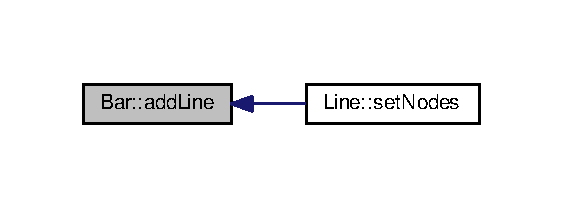
\includegraphics[width=270pt]{group___models_ga8cbd2f62d92e69ce6c8d561b682464b6_icgraph}
\end{center}
\end{figure}


\hypertarget{group___models_ga9cae2188fcc6cce41caa7898c64548d1}{}\index{Models@{Models}!Bar@{Bar}}
\index{Bar@{Bar}!Models@{Models}}
\paragraph[{Bar}]{\setlength{\rightskip}{0pt plus 5cm}Bar\+::\+Bar (
\begin{DoxyParamCaption}
{}
\end{DoxyParamCaption}
)}\label{group___models_ga9cae2188fcc6cce41caa7898c64548d1}
By default, bars are created filled with zeros. 

Definition at line \hyperlink{bar_8cpp_source_l00055}{55} of file \hyperlink{bar_8cpp_source}{bar.\+cpp}.

\hypertarget{group___models_gab1c5a81ad40dbc7ee745077b4f5c20d4}{}\index{Models@{Models}!Bar@{Bar}}
\index{Bar@{Bar}!Models@{Models}}
\paragraph[{Bar}]{\setlength{\rightskip}{0pt plus 5cm}Bar\+::\+Bar (
\begin{DoxyParamCaption}
\item[{complex$<$ double $>$}]{initial\+V, }
\item[{complex$<$ double $>$}]{initial\+Sh = {\ttfamily 0.0}, }
\item[{complex$<$ double $>$}]{initial\+Si = {\ttfamily 0.0}}
\end{DoxyParamCaption}
)}\label{group___models_gab1c5a81ad40dbc7ee745077b4f5c20d4}
This constructor is used when the bar needes to be initialized with pre-\/defined values. Note that the initial values will be applied to all phases.


\begin{DoxyParams}[1]{Parameters}
\mbox{\tt in}  & {\em initial\+V} & Initial voltage of the bar. \\
\hline
\mbox{\tt in}  & {\em initial\+Sh} & Initial shunt elements power. \\
\hline
\mbox{\tt in}  & {\em initial\+Si} & Initial injected power. \\
\hline
\end{DoxyParams}


Definition at line \hyperlink{bar_8cpp_source_l00078}{78} of file \hyperlink{bar_8cpp_source}{bar.\+cpp}.

\hypertarget{group___models_gad15c3af158d3b966c04be7e18cee5aea}{}\index{Models@{Models}!bounding\+Rect@{bounding\+Rect}}
\index{bounding\+Rect@{bounding\+Rect}!Models@{Models}}
\paragraph[{bounding\+Rect}]{\setlength{\rightskip}{0pt plus 5cm}Q\+Rect\+F Line\+::bounding\+Rect (
\begin{DoxyParamCaption}
{}
\end{DoxyParamCaption}
) const}\label{group___models_gad15c3af158d3b966c04be7e18cee5aea}


Definition at line \hyperlink{line_8cpp_source_l00286}{286} of file \hyperlink{line_8cpp_source}{line.\+cpp}.

\hypertarget{group___models_ga8279d8109019cc7e139e2023690496be}{}\index{Models@{Models}!bounding\+Rect@{bounding\+Rect}}
\index{bounding\+Rect@{bounding\+Rect}!Models@{Models}}
\paragraph[{bounding\+Rect}]{\setlength{\rightskip}{0pt plus 5cm}Q\+Rect\+F Bar\+::bounding\+Rect (
\begin{DoxyParamCaption}
{}
\end{DoxyParamCaption}
) const}\label{group___models_ga8279d8109019cc7e139e2023690496be}
\begin{DoxyReturn}{Returns}
The bar bounding rect. 
\end{DoxyReturn}


Definition at line \hyperlink{bar_8cpp_source_l00561}{561} of file \hyperlink{bar_8cpp_source}{bar.\+cpp}.



Here is the caller graph for this function\+:
\nopagebreak
\begin{figure}[H]
\begin{center}
\leavevmode
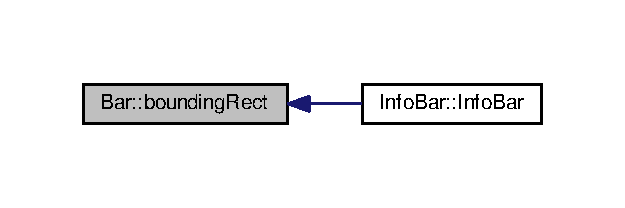
\includegraphics[width=300pt]{group___models_ga8279d8109019cc7e139e2023690496be_icgraph}
\end{center}
\end{figure}


\hypertarget{group___models_ga62623ad71df5279377cc69da90decc75}{}\index{Models@{Models}!from\+Json@{from\+Json}}
\index{from\+Json@{from\+Json}!Models@{Models}}
\paragraph[{from\+Json}]{\setlength{\rightskip}{0pt plus 5cm}void Line\+::from\+Json (
\begin{DoxyParamCaption}
\item[{Q\+Json\+Object \&}]{line\+Json}
\end{DoxyParamCaption}
)}\label{group___models_ga62623ad71df5279377cc69da90decc75}


Definition at line \hyperlink{line_8cpp_source_l00232}{232} of file \hyperlink{line_8cpp_source}{line.\+cpp}.

\hypertarget{group___models_ga1df62f03dd3a066ceaf6588ba6bb6004}{}\index{Models@{Models}!from\+Json@{from\+Json}}
\index{from\+Json@{from\+Json}!Models@{Models}}
\paragraph[{from\+Json}]{\setlength{\rightskip}{0pt plus 5cm}void Bar\+::from\+Json (
\begin{DoxyParamCaption}
\item[{Q\+Json\+Object \&}]{json\+Bar}
\end{DoxyParamCaption}
)}\label{group___models_ga1df62f03dd3a066ceaf6588ba6bb6004}

\begin{DoxyParams}[1]{Parameters}
\mbox{\tt in}  & {\em json\+Bar} & \\
\hline
\end{DoxyParams}


Definition at line \hyperlink{bar_8cpp_source_l00508}{508} of file \hyperlink{bar_8cpp_source}{bar.\+cpp}.

\hypertarget{group___models_gaf81e7055102816465bdf7e19afc2d547}{}\index{Models@{Models}!i@{i}}
\index{i@{i}!Models@{Models}}
\paragraph[{i}]{\setlength{\rightskip}{0pt plus 5cm}complex$<$ double $>$ Line\+::i (
\begin{DoxyParamCaption}
\item[{int32\+\_\+t}]{phase, }
\item[{{\bf Unit\+::\+Current\+Unit}}]{unit = {\ttfamily {\bf Unit\+::k\+Ampere}}}
\end{DoxyParamCaption}
)}\label{group___models_gaf81e7055102816465bdf7e19afc2d547}


Definition at line \hyperlink{line_8cpp_source_l00108}{108} of file \hyperlink{line_8cpp_source}{line.\+cpp}.

\hypertarget{group___models_ga8f71e477800134586652d283087ed373}{}\index{Models@{Models}!i\+Pu@{i\+Pu}}
\index{i\+Pu@{i\+Pu}!Models@{Models}}
\paragraph[{i\+Pu}]{\setlength{\rightskip}{0pt plus 5cm}complex$<$ double $>$ Line\+::i\+Pu (
\begin{DoxyParamCaption}
\item[{int32\+\_\+t}]{phase}
\end{DoxyParamCaption}
)}\label{group___models_ga8f71e477800134586652d283087ed373}


Definition at line \hyperlink{line_8cpp_source_l00126}{126} of file \hyperlink{line_8cpp_source}{line.\+cpp}.

\hypertarget{group___models_ga5fcee3f23eb50e34f730d602a3802b93}{}\index{Models@{Models}!item\+Change@{item\+Change}}
\index{item\+Change@{item\+Change}!Models@{Models}}
\paragraph[{item\+Change}]{\setlength{\rightskip}{0pt plus 5cm}Q\+Variant Line\+::item\+Change (
\begin{DoxyParamCaption}
\item[{Graphics\+Item\+Change}]{change, }
\item[{const Q\+Variant \&}]{value}
\end{DoxyParamCaption}
)}\label{group___models_ga5fcee3f23eb50e34f730d602a3802b93}


Definition at line \hyperlink{line_8cpp_source_l00304}{304} of file \hyperlink{line_8cpp_source}{line.\+cpp}.

\hypertarget{group___models_gad97a82d618ee0c51a9a36e44339c69e6}{}\index{Models@{Models}!item\+Change@{item\+Change}}
\index{item\+Change@{item\+Change}!Models@{Models}}
\paragraph[{item\+Change}]{\setlength{\rightskip}{0pt plus 5cm}Q\+Variant Bar\+::item\+Change (
\begin{DoxyParamCaption}
\item[{Graphics\+Item\+Change}]{change, }
\item[{const Q\+Variant \&}]{value}
\end{DoxyParamCaption}
)\hspace{0.3cm}{\ttfamily [protected]}}\label{group___models_gad97a82d618ee0c51a9a36e44339c69e6}
Used to handle item selection and geometry changes. \begin{DoxyReturn}{Returns}
Item change value; 
\end{DoxyReturn}


Definition at line \hyperlink{bar_8cpp_source_l00579}{579} of file \hyperlink{bar_8cpp_source}{bar.\+cpp}.



Here is the call graph for this function\+:
\nopagebreak
\begin{figure}[H]
\begin{center}
\leavevmode
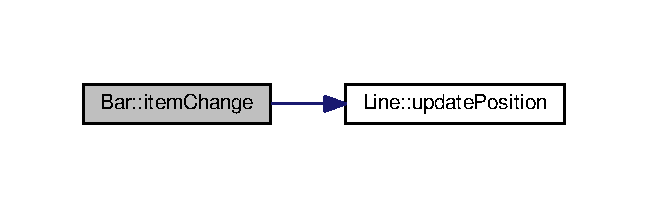
\includegraphics[width=311pt]{group___models_gad97a82d618ee0c51a9a36e44339c69e6_cgraph}
\end{center}
\end{figure}


\hypertarget{group___models_gae2e4500d0fa60dcc2ecb08b2c96954f9}{}\index{Models@{Models}!length@{length}}
\index{length@{length}!Models@{Models}}
\paragraph[{length}]{\setlength{\rightskip}{0pt plus 5cm}double Line\+::length (
\begin{DoxyParamCaption}
\item[{{\bf Unit\+::\+Length\+Unit}}]{unit = {\ttfamily {\bf Unit\+::k\+Meter}}}
\end{DoxyParamCaption}
)}\label{group___models_gae2e4500d0fa60dcc2ecb08b2c96954f9}


Definition at line \hyperlink{line_8cpp_source_l00144}{144} of file \hyperlink{line_8cpp_source}{line.\+cpp}.

\hypertarget{group___models_gacc11b8a429d8cdd63ba6803dff5602b3}{}\index{Models@{Models}!Line@{Line}}
\index{Line@{Line}!Models@{Models}}
\paragraph[{Line}]{\setlength{\rightskip}{0pt plus 5cm}Line\+::\+Line (
\begin{DoxyParamCaption}
{}
\end{DoxyParamCaption}
)}\label{group___models_gacc11b8a429d8cdd63ba6803dff5602b3}


Definition at line \hyperlink{line_8cpp_source_l00056}{56} of file \hyperlink{line_8cpp_source}{line.\+cpp}.

\hypertarget{group___models_ga84ddf17bee846a6f21c44d463252dd25}{}\index{Models@{Models}!loss@{loss}}
\index{loss@{loss}!Models@{Models}}
\paragraph[{loss}]{\setlength{\rightskip}{0pt plus 5cm}complex$<$ double $>$ Line\+::loss (
\begin{DoxyParamCaption}
\item[{int32\+\_\+t}]{phase}
\end{DoxyParamCaption}
)}\label{group___models_ga84ddf17bee846a6f21c44d463252dd25}


Definition at line \hyperlink{line_8cpp_source_l00135}{135} of file \hyperlink{line_8cpp_source}{line.\+cpp}.

\hypertarget{group___models_ga9a1fee5b1606ab0deedd04bdab99be70}{}\index{Models@{Models}!mouse\+Double\+Click\+Event@{mouse\+Double\+Click\+Event}}
\index{mouse\+Double\+Click\+Event@{mouse\+Double\+Click\+Event}!Models@{Models}}
\paragraph[{mouse\+Double\+Click\+Event}]{\setlength{\rightskip}{0pt plus 5cm}void Line\+::mouse\+Double\+Click\+Event (
\begin{DoxyParamCaption}
\item[{Q\+Graphics\+Scene\+Mouse\+Event $\ast$}]{event}
\end{DoxyParamCaption}
)\hspace{0.3cm}{\ttfamily [protected]}}\label{group___models_ga9a1fee5b1606ab0deedd04bdab99be70}

\begin{DoxyParams}{Parameters}
{\em event} & \\
\hline
\end{DoxyParams}


Definition at line \hyperlink{line_8cpp_source_l00331}{331} of file \hyperlink{line_8cpp_source}{line.\+cpp}.

\hypertarget{group___models_ga1945e7b4401fa9ad7475274d9fb12a72}{}\index{Models@{Models}!mouse\+Double\+Click\+Event@{mouse\+Double\+Click\+Event}}
\index{mouse\+Double\+Click\+Event@{mouse\+Double\+Click\+Event}!Models@{Models}}
\paragraph[{mouse\+Double\+Click\+Event}]{\setlength{\rightskip}{0pt plus 5cm}void Bar\+::mouse\+Double\+Click\+Event (
\begin{DoxyParamCaption}
\item[{Q\+Graphics\+Scene\+Mouse\+Event $\ast$}]{event}
\end{DoxyParamCaption}
)\hspace{0.3cm}{\ttfamily [protected]}}\label{group___models_ga1945e7b4401fa9ad7475274d9fb12a72}
Handles the double click event. 
\begin{DoxyParams}[1]{Parameters}
\mbox{\tt in}  & {\em event} & Event data. \\
\hline
\end{DoxyParams}


Definition at line \hyperlink{bar_8cpp_source_l00570}{570} of file \hyperlink{bar_8cpp_source}{bar.\+cpp}.

\hypertarget{group___models_ga0aa64aed379d434be5942edf572b444b}{}\index{Models@{Models}!paint@{paint}}
\index{paint@{paint}!Models@{Models}}
\paragraph[{paint}]{\setlength{\rightskip}{0pt plus 5cm}void Line\+::paint (
\begin{DoxyParamCaption}
\item[{Q\+Painter $\ast$}]{painter, }
\item[{const Q\+Style\+Option\+Graphics\+Item $\ast$}]{option, }
\item[{Q\+Widget $\ast$}]{widget}
\end{DoxyParamCaption}
)\hspace{0.3cm}{\ttfamily [protected]}}\label{group___models_ga0aa64aed379d434be5942edf572b444b}


Definition at line \hyperlink{line_8cpp_source_l00340}{340} of file \hyperlink{line_8cpp_source}{line.\+cpp}.

\hypertarget{group___models_gacbb6dbac607412c9c1f9dfcd0cd4d432}{}\index{Models@{Models}!paint@{paint}}
\index{paint@{paint}!Models@{Models}}
\paragraph[{paint}]{\setlength{\rightskip}{0pt plus 5cm}void Bar\+::paint (
\begin{DoxyParamCaption}
\item[{Q\+Painter $\ast$}]{painter, }
\item[{const Q\+Style\+Option\+Graphics\+Item $\ast$}]{option, }
\item[{Q\+Widget $\ast$}]{widget}
\end{DoxyParamCaption}
)\hspace{0.3cm}{\ttfamily [protected]}}\label{group___models_gacbb6dbac607412c9c1f9dfcd0cd4d432}
Overrided function that will paint the bar in the scene. 

Definition at line \hyperlink{bar_8cpp_source_l00617}{617} of file \hyperlink{bar_8cpp_source}{bar.\+cpp}.

\hypertarget{group___models_gabbc73ddedd3075c33ae5331bd7c9829f}{}\index{Models@{Models}!p\+No\+F@{p\+No\+F}}
\index{p\+No\+F@{p\+No\+F}!Models@{Models}}
\paragraph[{p\+No\+F}]{\setlength{\rightskip}{0pt plus 5cm}{\bf Bar} $\ast$ Line\+::p\+No\+F (
\begin{DoxyParamCaption}
{}
\end{DoxyParamCaption}
)}\label{group___models_gabbc73ddedd3075c33ae5331bd7c9829f}


Definition at line \hyperlink{line_8cpp_source_l00168}{168} of file \hyperlink{line_8cpp_source}{line.\+cpp}.



Here is the caller graph for this function\+:
\nopagebreak
\begin{figure}[H]
\begin{center}
\leavevmode
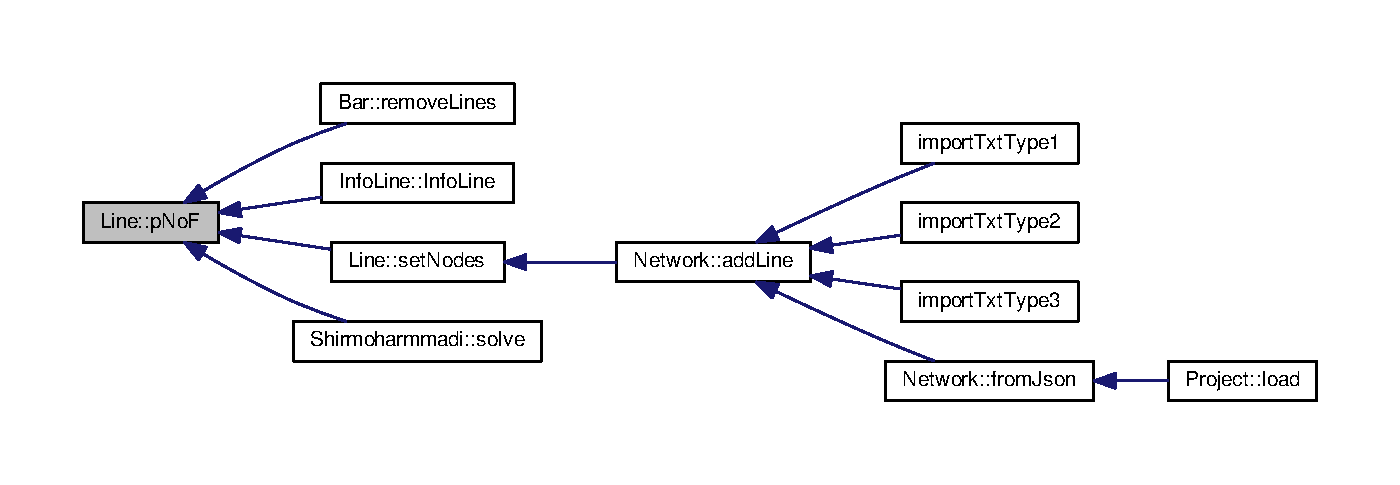
\includegraphics[width=274pt]{group___models_gabbc73ddedd3075c33ae5331bd7c9829f_icgraph}
\end{center}
\end{figure}


\hypertarget{group___models_gaeafd90e84ac2f8de2a879abe9e53eef3}{}\index{Models@{Models}!p\+No\+I@{p\+No\+I}}
\index{p\+No\+I@{p\+No\+I}!Models@{Models}}
\paragraph[{p\+No\+I}]{\setlength{\rightskip}{0pt plus 5cm}{\bf Bar} $\ast$ Line\+::p\+No\+I (
\begin{DoxyParamCaption}
{}
\end{DoxyParamCaption}
)}\label{group___models_gaeafd90e84ac2f8de2a879abe9e53eef3}


Definition at line \hyperlink{line_8cpp_source_l00160}{160} of file \hyperlink{line_8cpp_source}{line.\+cpp}.



Here is the caller graph for this function\+:
\nopagebreak
\begin{figure}[H]
\begin{center}
\leavevmode
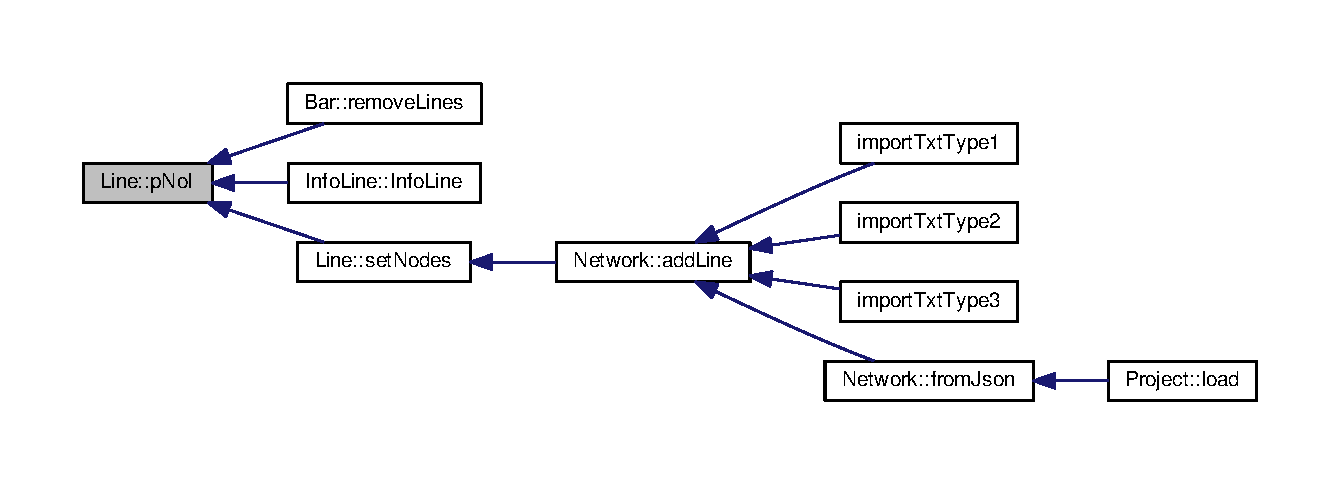
\includegraphics[width=271pt]{group___models_gaeafd90e84ac2f8de2a879abe9e53eef3_icgraph}
\end{center}
\end{figure}


\hypertarget{group___models_ga2536c0e5cb97fb627b3520826ece2c99}{}\index{Models@{Models}!remove\+Line@{remove\+Line}}
\index{remove\+Line@{remove\+Line}!Models@{Models}}
\paragraph[{remove\+Line}]{\setlength{\rightskip}{0pt plus 5cm}void Bar\+::remove\+Line (
\begin{DoxyParamCaption}
\item[{{\bf Line} $\ast$}]{line}
\end{DoxyParamCaption}
)}\label{group___models_ga2536c0e5cb97fb627b3520826ece2c99}

\begin{DoxyParams}[1]{Parameters}
\mbox{\tt in}  & {\em line} & \hyperlink{class_line}{Line} to be removed. \\
\hline
\end{DoxyParams}


Definition at line \hyperlink{bar_8cpp_source_l00427}{427} of file \hyperlink{bar_8cpp_source}{bar.\+cpp}.



Here is the caller graph for this function\+:
\nopagebreak
\begin{figure}[H]
\begin{center}
\leavevmode
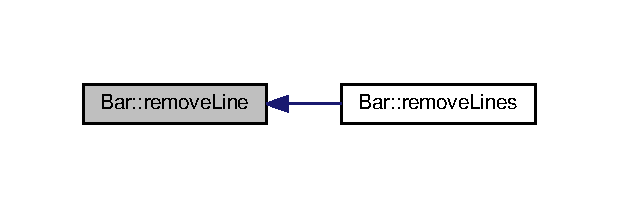
\includegraphics[width=297pt]{group___models_ga2536c0e5cb97fb627b3520826ece2c99_icgraph}
\end{center}
\end{figure}


\hypertarget{group___models_ga4ea1a2074cb45968d80d6add571884a4}{}\index{Models@{Models}!remove\+Lines@{remove\+Lines}}
\index{remove\+Lines@{remove\+Lines}!Models@{Models}}
\paragraph[{remove\+Lines}]{\setlength{\rightskip}{0pt plus 5cm}void Bar\+::remove\+Lines (
\begin{DoxyParamCaption}
{}
\end{DoxyParamCaption}
)}\label{group___models_ga4ea1a2074cb45968d80d6add571884a4}


Definition at line \hyperlink{bar_8cpp_source_l00437}{437} of file \hyperlink{bar_8cpp_source}{bar.\+cpp}.



Here is the call graph for this function\+:
\nopagebreak
\begin{figure}[H]
\begin{center}
\leavevmode
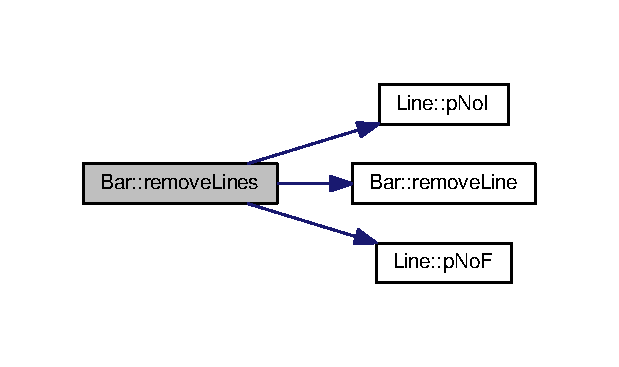
\includegraphics[width=297pt]{group___models_ga4ea1a2074cb45968d80d6add571884a4_cgraph}
\end{center}
\end{figure}


\hypertarget{group___models_gac8ddd4cb566d995b70b0f83146aa12b3}{}\index{Models@{Models}!r\+Si@{r\+Si}}
\index{r\+Si@{r\+Si}!Models@{Models}}
\paragraph[{r\+Si}]{\setlength{\rightskip}{0pt plus 5cm}complex$<$ double $>$ Bar\+::r\+Si (
\begin{DoxyParamCaption}
\item[{int32\+\_\+t}]{phase, }
\item[{{\bf Unit\+::\+Power\+Unit}}]{unit = {\ttfamily {\bf Unit\+::k\+V\+A}}}
\end{DoxyParamCaption}
)}\label{group___models_gac8ddd4cb566d995b70b0f83146aa12b3}
Returns the resulting injected power. Used by slack bar.


\begin{DoxyParams}[1]{Parameters}
\mbox{\tt in}  & {\em phase} & Phase (0, 1 or 2). \\
\hline
\mbox{\tt in}  & {\em unit} & \hyperlink{class_unit}{Unit}.\\
\hline
\end{DoxyParams}
\begin{DoxyReturn}{Returns}
Result injected power. 
\end{DoxyReturn}


Definition at line \hyperlink{bar_8cpp_source_l00352}{352} of file \hyperlink{bar_8cpp_source}{bar.\+cpp}.

\hypertarget{group___models_ga1fa1b99d17dd19fafcf8309aba4fc758}{}\index{Models@{Models}!r\+Si\+Pu@{r\+Si\+Pu}}
\index{r\+Si\+Pu@{r\+Si\+Pu}!Models@{Models}}
\paragraph[{r\+Si\+Pu}]{\setlength{\rightskip}{0pt plus 5cm}complex$<$ double $>$ Bar\+::r\+Si\+Pu (
\begin{DoxyParamCaption}
\item[{int32\+\_\+t}]{phase}
\end{DoxyParamCaption}
)}\label{group___models_ga1fa1b99d17dd19fafcf8309aba4fc758}
Return the resulting bar injected power, in per unit.


\begin{DoxyParams}[1]{Parameters}
\mbox{\tt in}  & {\em phase} & Phase (0, 1 or 2).\\
\hline
\end{DoxyParams}
\begin{DoxyReturn}{Returns}
Result injected power, in pu. 
\end{DoxyReturn}


Definition at line \hyperlink{bar_8cpp_source_l00408}{408} of file \hyperlink{bar_8cpp_source}{bar.\+cpp}.

\hypertarget{group___models_ga2d1f6bfbd8abaf168bb75bd8e5cd9b5e}{}\index{Models@{Models}!r\+V@{r\+V}}
\index{r\+V@{r\+V}!Models@{Models}}
\paragraph[{r\+V}]{\setlength{\rightskip}{0pt plus 5cm}complex$<$ double $>$ Bar\+::r\+V (
\begin{DoxyParamCaption}
\item[{int32\+\_\+t}]{phase, }
\item[{{\bf Unit\+::\+Voltage\+Unit}}]{unit = {\ttfamily {\bf Unit\+::k\+Volts}}}
\end{DoxyParamCaption}
)}\label{group___models_ga2d1f6bfbd8abaf168bb75bd8e5cd9b5e}
Returns the voltage of the bar after the calculations.


\begin{DoxyParams}[1]{Parameters}
\mbox{\tt in}  & {\em phase} & Phase (0, 1 or 2). \\
\hline
\mbox{\tt in}  & {\em unit} & \hyperlink{class_unit}{Unit} of the returned value.\\
\hline
\end{DoxyParams}
\begin{DoxyReturn}{Returns}
Result bar voltage. 
\end{DoxyReturn}


Definition at line \hyperlink{bar_8cpp_source_l00298}{298} of file \hyperlink{bar_8cpp_source}{bar.\+cpp}.

\hypertarget{group___models_ga7deee8820e2ee3e0db993a1e76b68700}{}\index{Models@{Models}!r\+V\+Pu@{r\+V\+Pu}}
\index{r\+V\+Pu@{r\+V\+Pu}!Models@{Models}}
\paragraph[{r\+V\+Pu}]{\setlength{\rightskip}{0pt plus 5cm}complex$<$ double $>$ Bar\+::r\+V\+Pu (
\begin{DoxyParamCaption}
\item[{int32\+\_\+t}]{phase}
\end{DoxyParamCaption}
)}\label{group___models_ga7deee8820e2ee3e0db993a1e76b68700}
Returns the resulting voltage in per unit.


\begin{DoxyParams}[1]{Parameters}
\mbox{\tt in}  & {\em phase} & Phase (0, 1 or 2).\\
\hline
\end{DoxyParams}
\begin{DoxyReturn}{Returns}
Result voltage in pu. 
\end{DoxyReturn}


Definition at line \hyperlink{bar_8cpp_source_l00341}{341} of file \hyperlink{bar_8cpp_source}{bar.\+cpp}.

\hypertarget{group___models_ga9e55b06dc3e385838fdd13d5580438ef}{}\index{Models@{Models}!set\+I@{set\+I}}
\index{set\+I@{set\+I}!Models@{Models}}
\paragraph[{set\+I}]{\setlength{\rightskip}{0pt plus 5cm}void Line\+::set\+I (
\begin{DoxyParamCaption}
\item[{int32\+\_\+t}]{phase, }
\item[{complex$<$ double $>$}]{new\+Current, }
\item[{{\bf Unit\+::\+Current\+Unit}}]{unit = {\ttfamily {\bf Unit\+::k\+Ampere}}}
\end{DoxyParamCaption}
)}\label{group___models_ga9e55b06dc3e385838fdd13d5580438ef}


Definition at line \hyperlink{line_8cpp_source_l00116}{116} of file \hyperlink{line_8cpp_source}{line.\+cpp}.

\hypertarget{group___models_ga950d0b8f5d167eda430c65ca7adadbb0}{}\index{Models@{Models}!set\+Length@{set\+Length}}
\index{set\+Length@{set\+Length}!Models@{Models}}
\paragraph[{set\+Length}]{\setlength{\rightskip}{0pt plus 5cm}void Line\+::set\+Length (
\begin{DoxyParamCaption}
\item[{double}]{new\+Length, }
\item[{{\bf Unit\+::\+Length\+Unit}}]{unit = {\ttfamily {\bf Unit\+::k\+Meter}}}
\end{DoxyParamCaption}
)}\label{group___models_ga950d0b8f5d167eda430c65ca7adadbb0}


Definition at line \hyperlink{line_8cpp_source_l00152}{152} of file \hyperlink{line_8cpp_source}{line.\+cpp}.

\hypertarget{group___models_gaeeab146e6c1d7d1a688a2764a9c9a170}{}\index{Models@{Models}!set\+Nodes@{set\+Nodes}}
\index{set\+Nodes@{set\+Nodes}!Models@{Models}}
\paragraph[{set\+Nodes}]{\setlength{\rightskip}{0pt plus 5cm}void Line\+::set\+Nodes (
\begin{DoxyParamCaption}
\item[{{\bf Bar} $\ast$}]{p\+No\+I, }
\item[{{\bf Bar} $\ast$}]{p\+No\+F}
\end{DoxyParamCaption}
)}\label{group___models_gaeeab146e6c1d7d1a688a2764a9c9a170}


Definition at line \hyperlink{line_8cpp_source_l00176}{176} of file \hyperlink{line_8cpp_source}{line.\+cpp}.



Here is the call graph for this function\+:
\nopagebreak
\begin{figure}[H]
\begin{center}
\leavevmode
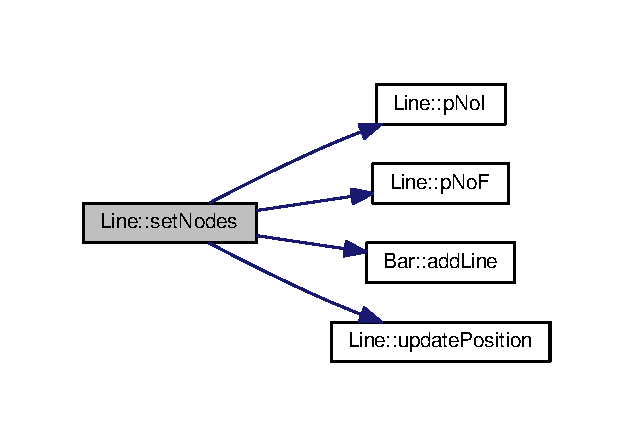
\includegraphics[width=304pt]{group___models_gaeeab146e6c1d7d1a688a2764a9c9a170_cgraph}
\end{center}
\end{figure}


\hypertarget{group___models_ga36d3d54b66584a0557c0c141f4636d4c}{}\index{Models@{Models}!set\+R\+Si@{set\+R\+Si}}
\index{set\+R\+Si@{set\+R\+Si}!Models@{Models}}
\paragraph[{set\+R\+Si}]{\setlength{\rightskip}{0pt plus 5cm}void Bar\+::set\+R\+Si (
\begin{DoxyParamCaption}
\item[{int32\+\_\+t}]{phase, }
\item[{complex$<$ double $>$}]{new\+Power, }
\item[{{\bf Unit\+::\+Power\+Unit}}]{unit = {\ttfamily {\bf Unit\+::k\+V\+A}}}
\end{DoxyParamCaption}
)}\label{group___models_ga36d3d54b66584a0557c0c141f4636d4c}
Set the resulting value for injected power.


\begin{DoxyParams}[1]{Parameters}
\mbox{\tt in}  & {\em phase} & Phase (0, 1 or 2). \\
\hline
\mbox{\tt in}  & {\em new\+Power} & New result injected power. \\
\hline
\mbox{\tt in}  & {\em unit} & Injected power unit. \\
\hline
\end{DoxyParams}


Definition at line \hyperlink{bar_8cpp_source_l00380}{380} of file \hyperlink{bar_8cpp_source}{bar.\+cpp}.

\hypertarget{group___models_ga2b2c5a373d87025e79d26aa9c4cea75a}{}\index{Models@{Models}!set\+R\+V@{set\+R\+V}}
\index{set\+R\+V@{set\+R\+V}!Models@{Models}}
\paragraph[{set\+R\+V}]{\setlength{\rightskip}{0pt plus 5cm}void Bar\+::set\+R\+V (
\begin{DoxyParamCaption}
\item[{int32\+\_\+t}]{phase, }
\item[{complex$<$ double $>$}]{result\+Voltage, }
\item[{{\bf Unit\+::\+Voltage\+Unit}}]{unit = {\ttfamily {\bf Unit\+::k\+Volts}}}
\end{DoxyParamCaption}
)}\label{group___models_ga2b2c5a373d87025e79d26aa9c4cea75a}
Set the result voltage after calculations.


\begin{DoxyParams}[1]{Parameters}
\mbox{\tt in}  & {\em phase} & Phase (0, 1 or 2). \\
\hline
\mbox{\tt in}  & {\em result\+Voltage} & New result voltage.\\
\hline
\mbox{\tt in}  & {\em unit} & Result unit. \\
\hline
\end{DoxyParams}


Definition at line \hyperlink{bar_8cpp_source_l00321}{321} of file \hyperlink{bar_8cpp_source}{bar.\+cpp}.

\hypertarget{group___models_ga207abd3d0649a488e3c44cf2a501ed23}{}\index{Models@{Models}!set\+Sh@{set\+Sh}}
\index{set\+Sh@{set\+Sh}!Models@{Models}}
\paragraph[{set\+Sh}]{\setlength{\rightskip}{0pt plus 5cm}void Bar\+::set\+Sh (
\begin{DoxyParamCaption}
\item[{int32\+\_\+t}]{phase, }
\item[{complex$<$ double $>$}]{new\+Power, }
\item[{{\bf Unit\+::\+Power\+Unit}}]{unit = {\ttfamily {\bf Unit\+::k\+V\+A}}}
\end{DoxyParamCaption}
)}\label{group___models_ga207abd3d0649a488e3c44cf2a501ed23}
Set the shunt element injected power.


\begin{DoxyParams}[1]{Parameters}
\mbox{\tt in}  & {\em phase} & Phase (0, 1 or 2). \\
\hline
\mbox{\tt in}  & {\em new\+Power} & Shunt power. \\
\hline
\mbox{\tt in}  & {\em unit} & Shunt power unit. \\
\hline
\end{DoxyParams}


Definition at line \hyperlink{bar_8cpp_source_l00192}{192} of file \hyperlink{bar_8cpp_source}{bar.\+cpp}.

\hypertarget{group___models_ga74e510be49e50e4c14550b32e1dc92f9}{}\index{Models@{Models}!set\+Si@{set\+Si}}
\index{set\+Si@{set\+Si}!Models@{Models}}
\paragraph[{set\+Si}]{\setlength{\rightskip}{0pt plus 5cm}void Bar\+::set\+Si (
\begin{DoxyParamCaption}
\item[{int32\+\_\+t}]{phase, }
\item[{complex$<$ double $>$}]{new\+Power, }
\item[{{\bf Unit\+::\+Power\+Unit}}]{unit = {\ttfamily {\bf Unit\+::k\+V\+A}}}
\end{DoxyParamCaption}
)}\label{group___models_ga74e510be49e50e4c14550b32e1dc92f9}
Set the injected power at the bar. Generated power is negative, load is positive.


\begin{DoxyParams}[1]{Parameters}
\mbox{\tt in}  & {\em phase} & Phase (0, 1 or 2). \\
\hline
\mbox{\tt in}  & {\em new\+Power} & New injected power. \\
\hline
\mbox{\tt in}  & {\em unit} & New injected power unit. \\
\hline
\end{DoxyParams}


Definition at line \hyperlink{bar_8cpp_source_l00259}{259} of file \hyperlink{bar_8cpp_source}{bar.\+cpp}.

\hypertarget{group___models_ga9b6fbc92674bfcdc9d5090795ab335a6}{}\index{Models@{Models}!set\+V@{set\+V}}
\index{set\+V@{set\+V}!Models@{Models}}
\paragraph[{set\+V}]{\setlength{\rightskip}{0pt plus 5cm}void Bar\+::set\+V (
\begin{DoxyParamCaption}
\item[{int32\+\_\+t}]{phase, }
\item[{complex$<$ double $>$}]{new\+Voltage, }
\item[{{\bf Unit\+::\+Voltage\+Unit}}]{unit = {\ttfamily {\bf Unit\+::k\+Volts}}}
\end{DoxyParamCaption}
)}\label{group___models_ga9b6fbc92674bfcdc9d5090795ab335a6}
Set the initial voltage of the selected phase.


\begin{DoxyParams}[1]{Parameters}
\mbox{\tt in}  & {\em phase} & Phase (0, 1 or 2). \\
\hline
\mbox{\tt in}  & {\em new\+Voltage} & New voltage. \\
\hline
\mbox{\tt in}  & {\em unit} & \hyperlink{class_unit}{Unit} of the new voltage. \\
\hline
\end{DoxyParams}


Definition at line \hyperlink{bar_8cpp_source_l00133}{133} of file \hyperlink{bar_8cpp_source}{bar.\+cpp}.

\hypertarget{group___models_ga409df7d11f5c5d594a13fb2f74b3b9e0}{}\index{Models@{Models}!set\+Z@{set\+Z}}
\index{set\+Z@{set\+Z}!Models@{Models}}
\paragraph[{set\+Z}]{\setlength{\rightskip}{0pt plus 5cm}void Line\+::set\+Z (
\begin{DoxyParamCaption}
\item[{int32\+\_\+t}]{index, }
\item[{complex$<$ double $>$}]{new\+Impedance, }
\item[{{\bf Unit\+::\+Impedance\+Unit}}]{unit = {\ttfamily {\bf Unit\+::k\+Ohm}}}
\end{DoxyParamCaption}
)}\label{group___models_ga409df7d11f5c5d594a13fb2f74b3b9e0}


Definition at line \hyperlink{line_8cpp_source_l00091}{91} of file \hyperlink{line_8cpp_source}{line.\+cpp}.

\hypertarget{group___models_gac188071bf5f165b0acdaa4c8af82355c}{}\index{Models@{Models}!sh@{sh}}
\index{sh@{sh}!Models@{Models}}
\paragraph[{sh}]{\setlength{\rightskip}{0pt plus 5cm}complex$<$ double $>$ Bar\+::sh (
\begin{DoxyParamCaption}
\item[{int32\+\_\+t}]{phase, }
\item[{{\bf Unit\+::\+Power\+Unit}}]{unit = {\ttfamily {\bf Unit\+::k\+V\+A}}}
\end{DoxyParamCaption}
)}\label{group___models_gac188071bf5f165b0acdaa4c8af82355c}
Power injected by the shunt element.


\begin{DoxyParams}[1]{Parameters}
\mbox{\tt in}  & {\em phase} & Phase (0, 1 or 2). \\
\hline
\mbox{\tt in}  & {\em unit} & \hyperlink{class_unit}{Unit} of the returned value (default to V\+A).\\
\hline
\end{DoxyParams}
\begin{DoxyReturn}{Returns}
The power of the shunt element. 
\end{DoxyReturn}


Definition at line \hyperlink{bar_8cpp_source_l00164}{164} of file \hyperlink{bar_8cpp_source}{bar.\+cpp}.

\hypertarget{group___models_gaf1736b829a643d99052ef6428ddd5b16}{}\index{Models@{Models}!shape@{shape}}
\index{shape@{shape}!Models@{Models}}
\paragraph[{shape}]{\setlength{\rightskip}{0pt plus 5cm}Q\+Painter\+Path Line\+::shape (
\begin{DoxyParamCaption}
{}
\end{DoxyParamCaption}
) const}\label{group___models_gaf1736b829a643d99052ef6428ddd5b16}


Definition at line \hyperlink{line_8cpp_source_l00294}{294} of file \hyperlink{line_8cpp_source}{line.\+cpp}.

\hypertarget{group___models_ga7df2ed5705f06c0cf2937d25102ca847}{}\index{Models@{Models}!sh\+Pu@{sh\+Pu}}
\index{sh\+Pu@{sh\+Pu}!Models@{Models}}
\paragraph[{sh\+Pu}]{\setlength{\rightskip}{0pt plus 5cm}complex$<$ double $>$ Bar\+::sh\+Pu (
\begin{DoxyParamCaption}
\item[{int32\+\_\+t}]{phase}
\end{DoxyParamCaption}
)}\label{group___models_ga7df2ed5705f06c0cf2937d25102ca847}
Shunt element power in pu. The power base is gettered from the network in which the bar is.


\begin{DoxyParams}[1]{Parameters}
\mbox{\tt in}  & {\em phase} & Phase (0, 1 or 2).\\
\hline
\end{DoxyParams}
\begin{DoxyReturn}{Returns}
Shunt power in per unit. 
\end{DoxyReturn}


Definition at line \hyperlink{bar_8cpp_source_l00220}{220} of file \hyperlink{bar_8cpp_source}{bar.\+cpp}.

\hypertarget{group___models_ga02bbc279f1e133f66b12ee21e7bebcd8}{}\index{Models@{Models}!si@{si}}
\index{si@{si}!Models@{Models}}
\paragraph[{si}]{\setlength{\rightskip}{0pt plus 5cm}complex$<$ double $>$ Bar\+::si (
\begin{DoxyParamCaption}
\item[{int32\+\_\+t}]{phase, }
\item[{{\bf Unit\+::\+Power\+Unit}}]{unit = {\ttfamily {\bf Unit\+::k\+V\+A}}}
\end{DoxyParamCaption}
)}\label{group___models_ga02bbc279f1e133f66b12ee21e7bebcd8}
Injected power at the bar. Generated power is negative, load is positive.


\begin{DoxyParams}[1]{Parameters}
\mbox{\tt in}  & {\em phase} & Phase (0, 1 or 2). \\
\hline
\mbox{\tt in}  & {\em unit} & Power unit.\\
\hline
\end{DoxyParams}
\begin{DoxyReturn}{Returns}
Injected power. 
\end{DoxyReturn}


Definition at line \hyperlink{bar_8cpp_source_l00231}{231} of file \hyperlink{bar_8cpp_source}{bar.\+cpp}.

\hypertarget{group___models_ga8ac94a6b5f69417da962a7d87361b416}{}\index{Models@{Models}!si\+Pu@{si\+Pu}}
\index{si\+Pu@{si\+Pu}!Models@{Models}}
\paragraph[{si\+Pu}]{\setlength{\rightskip}{0pt plus 5cm}complex$<$ double $>$ Bar\+::si\+Pu (
\begin{DoxyParamCaption}
\item[{int32\+\_\+t}]{phase}
\end{DoxyParamCaption}
)}\label{group___models_ga8ac94a6b5f69417da962a7d87361b416}
Returns the injected power in per unit.


\begin{DoxyParams}[1]{Parameters}
\mbox{\tt in}  & {\em phase} & Phase (0, 1 or 2).\\
\hline
\end{DoxyParams}
\begin{DoxyReturn}{Returns}
Injected power in per unit. 
\end{DoxyReturn}


Definition at line \hyperlink{bar_8cpp_source_l00287}{287} of file \hyperlink{bar_8cpp_source}{bar.\+cpp}.

\hypertarget{group___models_ga4effa7a96db465ea6e01135d5a010739}{}\index{Models@{Models}!to\+Json@{to\+Json}}
\index{to\+Json@{to\+Json}!Models@{Models}}
\paragraph[{to\+Json}]{\setlength{\rightskip}{0pt plus 5cm}Q\+Json\+Object Line\+::to\+Json (
\begin{DoxyParamCaption}
{}
\end{DoxyParamCaption}
)}\label{group___models_ga4effa7a96db465ea6e01135d5a010739}


Definition at line \hyperlink{line_8cpp_source_l00193}{193} of file \hyperlink{line_8cpp_source}{line.\+cpp}.

\hypertarget{group___models_ga3eb84c42b687db6cd98e11b8bd38c86e}{}\index{Models@{Models}!to\+Json@{to\+Json}}
\index{to\+Json@{to\+Json}!Models@{Models}}
\paragraph[{to\+Json}]{\setlength{\rightskip}{0pt plus 5cm}Q\+Json\+Object Bar\+::to\+Json (
\begin{DoxyParamCaption}
{}
\end{DoxyParamCaption}
)}\label{group___models_ga3eb84c42b687db6cd98e11b8bd38c86e}
\begin{DoxyReturn}{Returns}
Return json object filled with bar data. 
\end{DoxyReturn}


Definition at line \hyperlink{bar_8cpp_source_l00450}{450} of file \hyperlink{bar_8cpp_source}{bar.\+cpp}.

\hypertarget{group___models_ga8fdb12651d4bc592616d241386b066b3}{}\index{Models@{Models}!update\+Position@{update\+Position}}
\index{update\+Position@{update\+Position}!Models@{Models}}
\paragraph[{update\+Position}]{\setlength{\rightskip}{0pt plus 5cm}void Line\+::update\+Position (
\begin{DoxyParamCaption}
{}
\end{DoxyParamCaption}
)}\label{group___models_ga8fdb12651d4bc592616d241386b066b3}


Definition at line \hyperlink{line_8cpp_source_l00267}{267} of file \hyperlink{line_8cpp_source}{line.\+cpp}.



Here is the caller graph for this function\+:
\nopagebreak
\begin{figure}[H]
\begin{center}
\leavevmode
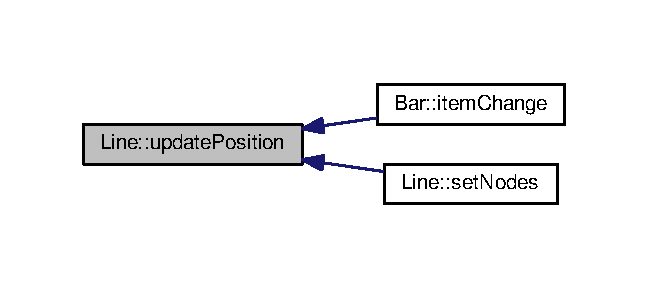
\includegraphics[width=311pt]{group___models_ga8fdb12651d4bc592616d241386b066b3_icgraph}
\end{center}
\end{figure}


\hypertarget{group___models_ga1e6f2daec86407118656d88170d1adc2}{}\index{Models@{Models}!v@{v}}
\index{v@{v}!Models@{Models}}
\paragraph[{v}]{\setlength{\rightskip}{0pt plus 5cm}complex$<$ double $>$ Bar\+::v (
\begin{DoxyParamCaption}
\item[{int32\+\_\+t}]{phase, }
\item[{{\bf Unit\+::\+Voltage\+Unit}}]{unit = {\ttfamily {\bf Unit\+::k\+Volts}}}
\end{DoxyParamCaption}
)}\label{group___models_ga1e6f2daec86407118656d88170d1adc2}
Returns the initial voltage in the specified unit.


\begin{DoxyParams}[1]{Parameters}
\mbox{\tt in}  & {\em phase} & Phase (0, 1 or 2). \\
\hline
\mbox{\tt in}  & {\em unit} & \hyperlink{class_unit}{Unit} of the voltage (default is Volts).\\
\hline
\end{DoxyParams}
\begin{DoxyReturn}{Returns}
Voltage of phase {\bfseries phase}. 
\end{DoxyReturn}


Definition at line \hyperlink{bar_8cpp_source_l00110}{110} of file \hyperlink{bar_8cpp_source}{bar.\+cpp}.

\hypertarget{group___models_ga1c54bd76b2f620d970ddfed8cdae4116}{}\index{Models@{Models}!v\+Pu@{v\+Pu}}
\index{v\+Pu@{v\+Pu}!Models@{Models}}
\paragraph[{v\+Pu}]{\setlength{\rightskip}{0pt plus 5cm}complex$<$ double $>$ Bar\+::v\+Pu (
\begin{DoxyParamCaption}
\item[{int32\+\_\+t}]{phase}
\end{DoxyParamCaption}
)}\label{group___models_ga1c54bd76b2f620d970ddfed8cdae4116}
Returns the initial voltage converted to per unit, where the base voltage is the network base voltage.


\begin{DoxyParams}[1]{Parameters}
\mbox{\tt in}  & {\em phase} & Phase (0, 1 or 2).\\
\hline
\end{DoxyParams}
\begin{DoxyReturn}{Returns}
The initial voltage, in per unit. 
\end{DoxyReturn}


Definition at line \hyperlink{bar_8cpp_source_l00153}{153} of file \hyperlink{bar_8cpp_source}{bar.\+cpp}.

\hypertarget{group___models_gab5370574fd93e13eb11742f7753fe1f1}{}\index{Models@{Models}!z@{z}}
\index{z@{z}!Models@{Models}}
\paragraph[{z}]{\setlength{\rightskip}{0pt plus 5cm}complex$<$ double $>$ Line\+::z (
\begin{DoxyParamCaption}
\item[{int32\+\_\+t}]{index, }
\item[{{\bf Unit\+::\+Impedance\+Unit}}]{unit = {\ttfamily {\bf Unit\+::k\+Ohm}}}
\end{DoxyParamCaption}
)}\label{group___models_gab5370574fd93e13eb11742f7753fe1f1}


Definition at line \hyperlink{line_8cpp_source_l00083}{83} of file \hyperlink{line_8cpp_source}{line.\+cpp}.

\hypertarget{group___models_ga139698332327a712f6c02d96fe73fbee}{}\index{Models@{Models}!z\+Pu@{z\+Pu}}
\index{z\+Pu@{z\+Pu}!Models@{Models}}
\paragraph[{z\+Pu}]{\setlength{\rightskip}{0pt plus 5cm}complex$<$ double $>$ Line\+::z\+Pu (
\begin{DoxyParamCaption}
\item[{int32\+\_\+t}]{index}
\end{DoxyParamCaption}
)}\label{group___models_ga139698332327a712f6c02d96fe73fbee}


Definition at line \hyperlink{line_8cpp_source_l00100}{100} of file \hyperlink{line_8cpp_source}{line.\+cpp}.

\hypertarget{group___models_ga9c7ebea0c189423591741ac438985316}{}\index{Models@{Models}!````~Bar@{$\sim$\+Bar}}
\index{````~Bar@{$\sim$\+Bar}!Models@{Models}}
\paragraph[{$\sim$\+Bar}]{\setlength{\rightskip}{0pt plus 5cm}Bar\+::$\sim$\+Bar (
\begin{DoxyParamCaption}
{}
\end{DoxyParamCaption}
)\hspace{0.3cm}{\ttfamily [virtual]}}\label{group___models_ga9c7ebea0c189423591741ac438985316}
\hyperlink{class_bar}{Bar} destructor. 

Definition at line \hyperlink{bar_8cpp_source_l00103}{103} of file \hyperlink{bar_8cpp_source}{bar.\+cpp}.

\hypertarget{group___models_gaabe85f48d22d92b62257091f48174fac}{}\index{Models@{Models}!````~Line@{$\sim$\+Line}}
\index{````~Line@{$\sim$\+Line}!Models@{Models}}
\paragraph[{$\sim$\+Line}]{\setlength{\rightskip}{0pt plus 5cm}Line\+::$\sim$\+Line (
\begin{DoxyParamCaption}
{}
\end{DoxyParamCaption}
)}\label{group___models_gaabe85f48d22d92b62257091f48174fac}


Definition at line \hyperlink{line_8cpp_source_l00078}{78} of file \hyperlink{line_8cpp_source}{line.\+cpp}.



\subsubsection{Variable Documentation}
\hypertarget{group___models_ga9919592c0397ed41448dfb20b607d738}{}\index{Models@{Models}!k\+Invalid\+Id@{k\+Invalid\+Id}}
\index{k\+Invalid\+Id@{k\+Invalid\+Id}!Models@{Models}}
\paragraph[{k\+Invalid\+Id}]{\setlength{\rightskip}{0pt plus 5cm}const int32\+\_\+t Bar\+::k\+Invalid\+Id = -\/1\hspace{0.3cm}{\ttfamily [static]}}\label{group___models_ga9919592c0397ed41448dfb20b607d738}
This value is used to determine if a bar has been correctly initialized and to check if bar data is valid; 

Definition at line \hyperlink{bar_8h_source_l00126}{126} of file \hyperlink{bar_8h_source}{bar.\+h}.

\hypertarget{group___models_gadc334bd07c6126abc56e531d7e3e72b4}{}\index{Models@{Models}!k\+Invalid\+Node@{k\+Invalid\+Node}}
\index{k\+Invalid\+Node@{k\+Invalid\+Node}!Models@{Models}}
\paragraph[{k\+Invalid\+Node}]{\setlength{\rightskip}{0pt plus 5cm}const int32\+\_\+t Line\+::k\+Invalid\+Node = -\/1\hspace{0.3cm}{\ttfamily [static]}}\label{group___models_gadc334bd07c6126abc56e531d7e3e72b4}


Definition at line \hyperlink{line_8h_source_l00082}{82} of file \hyperlink{line_8h_source}{line.\+h}.


\hypertarget{group___window}{}\subsection{Window}
\label{group___window}\index{Window@{Window}}
\subsubsection*{Files}
\begin{DoxyCompactItemize}
\item 
file \hyperlink{quickflow_8cpp}{quickflow.\+cpp}
\begin{DoxyCompactList}\small\item\em Main window class implementation. \end{DoxyCompactList}\item 
file \hyperlink{quickflow_8h}{quickflow.\+h}
\begin{DoxyCompactList}\small\item\em Main window class definition. \end{DoxyCompactList}\item 
file \hyperlink{about_8cpp}{about.\+cpp}
\begin{DoxyCompactList}\small\item\em Implementation of the \hyperlink{class_about}{About} dialog class. \end{DoxyCompactList}\item 
file \hyperlink{about_8h}{about.\+h}
\begin{DoxyCompactList}\small\item\em \hyperlink{class_about}{About} class definition. \end{DoxyCompactList}\item 
file \hyperlink{newproject_8cpp}{newproject.\+cpp}
\begin{DoxyCompactList}\small\item\em Implementation of the \hyperlink{class_new_project}{New\+Project} class. \end{DoxyCompactList}\item 
file \hyperlink{newproject_8h}{newproject.\+h}
\begin{DoxyCompactList}\small\item\em \hyperlink{class_new_project}{New\+Project} class definition. \end{DoxyCompactList}\end{DoxyCompactItemize}
\subsubsection*{Namespaces}
\begin{DoxyCompactItemize}
\item 
 \hyperlink{namespace_ui}{Ui}
\end{DoxyCompactItemize}
\subsubsection*{Classes}
\begin{DoxyCompactItemize}
\item 
class \hyperlink{class_quick_flow}{Quick\+Flow}
\begin{DoxyCompactList}\small\item\em This is the main window of the software. \end{DoxyCompactList}\item 
class \hyperlink{class_about}{About}
\begin{DoxyCompactList}\small\item\em Window to display information about the software. \end{DoxyCompactList}\item 
class \hyperlink{class_new_project}{New\+Project}
\begin{DoxyCompactList}\small\item\em Gets user input to create a new project. \end{DoxyCompactList}\end{DoxyCompactItemize}
\subsubsection*{Functions}
\begin{DoxyCompactItemize}
\item 
\hyperlink{group___window_ga7689e2608835392fce3f4c95a7a542db}{Quick\+Flow\+::\+Quick\+Flow} (Q\+Widget $\ast$parent=0)
\begin{DoxyCompactList}\small\item\em Constructor. \end{DoxyCompactList}\item 
\hyperlink{group___window_ga985823a0db64246b3a15eed2f397e0a4}{Quick\+Flow\+::$\sim$\+Quick\+Flow} ()
\begin{DoxyCompactList}\small\item\em Destructor. \end{DoxyCompactList}\item 
bool \hyperlink{group___window_ga5d9148467ef65c48419bf020ee107a45}{Quick\+Flow\+::is\+Altered} ()
\begin{DoxyCompactList}\small\item\em Check if project is altered Check the altered flag. \end{DoxyCompactList}\item 
void \hyperlink{group___window_ga4b63ea5ca52a9eea14db0a22b5a133f8}{Quick\+Flow\+::set\+Altered} (bool altered)
\begin{DoxyCompactList}\small\item\em Set the altered flag. \end{DoxyCompactList}\item 
void \hyperlink{group___window_gac8cc1bb329961a0781ffed7b6f2ab402}{Quick\+Flow\+::close\+Event} (Q\+Close\+Event $\ast$event) Q\+\_\+\+D\+E\+C\+L\+\_\+\+O\+V\+E\+R\+R\+I\+D\+E
\begin{DoxyCompactList}\small\item\em Handles software termination. \end{DoxyCompactList}\item 
\hyperlink{group___window_gab79599ebbcdeffe0a96e00f010e64177}{About\+::\+About} (Q\+Widget $\ast$parent=0)
\begin{DoxyCompactList}\small\item\em Constructor. \end{DoxyCompactList}\item 
\hyperlink{group___window_gace60197b1b610998908036ee1f802204}{About\+::$\sim$\+About} ()
\begin{DoxyCompactList}\small\item\em Destructor. \end{DoxyCompactList}\item 
\hyperlink{group___window_ga011ff7a4c380f74bdafa4fdaed510c42}{New\+Project\+::\+New\+Project} (Q\+Widget $\ast$parent=0)
\begin{DoxyCompactList}\small\item\em \hyperlink{class_new_project}{New\+Project} constructor. \end{DoxyCompactList}\item 
\hyperlink{group___window_gae65155941598f4272f3df0b2f1428c78}{New\+Project\+::$\sim$\+New\+Project} ()
\begin{DoxyCompactList}\small\item\em Destructor. \end{DoxyCompactList}\end{DoxyCompactItemize}
\subsubsection*{Variables}
\begin{DoxyCompactItemize}
\item 
static const Q\+String \hyperlink{group___window_gabfc3b1280bdae9a9c046d56b1459ab99}{Quick\+Flow\+::k\+Version} = \char`\"{}0.\+0.\+5\char`\"{}
\end{DoxyCompactItemize}


\subsubsection{Detailed Description}


\subsubsection{Function Documentation}
\hypertarget{group___window_gab79599ebbcdeffe0a96e00f010e64177}{}\index{Window@{Window}!About@{About}}
\index{About@{About}!Window@{Window}}
\paragraph[{About}]{\setlength{\rightskip}{0pt plus 5cm}About\+::\+About (
\begin{DoxyParamCaption}
\item[{Q\+Widget $\ast$}]{parent = {\ttfamily 0}}
\end{DoxyParamCaption}
)\hspace{0.3cm}{\ttfamily [explicit]}}\label{group___window_gab79599ebbcdeffe0a96e00f010e64177}
Create the class.


\begin{DoxyParams}[1]{Parameters}
\mbox{\tt in}  & {\em parent} & Parent widget. \\
\hline
\end{DoxyParams}


Definition at line \hyperlink{about_8cpp_source_l00049}{49} of file \hyperlink{about_8cpp_source}{about.\+cpp}.

\hypertarget{group___window_gac8cc1bb329961a0781ffed7b6f2ab402}{}\index{Window@{Window}!close\+Event@{close\+Event}}
\index{close\+Event@{close\+Event}!Window@{Window}}
\paragraph[{close\+Event}]{\setlength{\rightskip}{0pt plus 5cm}void Quick\+Flow\+::close\+Event (
\begin{DoxyParamCaption}
\item[{Q\+Close\+Event $\ast$}]{event}
\end{DoxyParamCaption}
)\hspace{0.3cm}{\ttfamily [protected]}}\label{group___window_gac8cc1bb329961a0781ffed7b6f2ab402}
This event will check if there is something to be saved and, if so, confirm the user will to save or discard the changes. 

Definition at line \hyperlink{quickflow_8cpp_source_l00631}{631} of file \hyperlink{quickflow_8cpp_source}{quickflow.\+cpp}.

\hypertarget{group___window_ga5d9148467ef65c48419bf020ee107a45}{}\index{Window@{Window}!is\+Altered@{is\+Altered}}
\index{is\+Altered@{is\+Altered}!Window@{Window}}
\paragraph[{is\+Altered}]{\setlength{\rightskip}{0pt plus 5cm}bool Quick\+Flow\+::is\+Altered (
\begin{DoxyParamCaption}
{}
\end{DoxyParamCaption}
)}\label{group___window_ga5d9148467ef65c48419bf020ee107a45}
This flag is cleared everytime the project is saved and is set when any alteration occurs.

\begin{DoxyReturn}{Returns}
true if project has been altered, false otherwise.
\end{DoxyReturn}
\begin{DoxyNote}{Note}
Must be replaced by Qt undo framework. 
\end{DoxyNote}


Definition at line \hyperlink{quickflow_8cpp_source_l00111}{111} of file \hyperlink{quickflow_8cpp_source}{quickflow.\+cpp}.

\hypertarget{group___window_ga011ff7a4c380f74bdafa4fdaed510c42}{}\index{Window@{Window}!New\+Project@{New\+Project}}
\index{New\+Project@{New\+Project}!Window@{Window}}
\paragraph[{New\+Project}]{\setlength{\rightskip}{0pt plus 5cm}New\+Project\+::\+New\+Project (
\begin{DoxyParamCaption}
\item[{Q\+Widget $\ast$}]{parent = {\ttfamily 0}}
\end{DoxyParamCaption}
)\hspace{0.3cm}{\ttfamily [explicit]}}\label{group___window_ga011ff7a4c380f74bdafa4fdaed510c42}

\begin{DoxyParams}[1]{Parameters}
\mbox{\tt in}  & {\em parent} & Parent widget. \\
\hline
\end{DoxyParams}


Definition at line \hyperlink{newproject_8cpp_source_l00056}{56} of file \hyperlink{newproject_8cpp_source}{newproject.\+cpp}.

\hypertarget{group___window_ga7689e2608835392fce3f4c95a7a542db}{}\index{Window@{Window}!Quick\+Flow@{Quick\+Flow}}
\index{Quick\+Flow@{Quick\+Flow}!Window@{Window}}
\paragraph[{Quick\+Flow}]{\setlength{\rightskip}{0pt plus 5cm}Quick\+Flow\+::\+Quick\+Flow (
\begin{DoxyParamCaption}
\item[{Q\+Widget $\ast$}]{parent = {\ttfamily 0}}
\end{DoxyParamCaption}
)\hspace{0.3cm}{\ttfamily [explicit]}}\label{group___window_ga7689e2608835392fce3f4c95a7a542db}
Here, we must initialize the user interface and load the software settings, updating or creating a new set of configurantion if needed.


\begin{DoxyParams}[1]{Parameters}
\mbox{\tt in}  & {\em parent} & Parent widget. \\
\hline
\end{DoxyParams}


Definition at line \hyperlink{quickflow_8cpp_source_l00066}{66} of file \hyperlink{quickflow_8cpp_source}{quickflow.\+cpp}.

\hypertarget{group___window_ga4b63ea5ca52a9eea14db0a22b5a133f8}{}\index{Window@{Window}!set\+Altered@{set\+Altered}}
\index{set\+Altered@{set\+Altered}!Window@{Window}}
\paragraph[{set\+Altered}]{\setlength{\rightskip}{0pt plus 5cm}void Quick\+Flow\+::set\+Altered (
\begin{DoxyParamCaption}
\item[{bool}]{altered}
\end{DoxyParamCaption}
)}\label{group___window_ga4b63ea5ca52a9eea14db0a22b5a133f8}
If {\bfseries altered} is true, enable the save action and set altered\+\_\+ to true. If false, disable the save action.


\begin{DoxyParams}[1]{Parameters}
\mbox{\tt in}  & {\em altered} & Must be replaced by Qt undo framework. \\
\hline
\end{DoxyParams}


Definition at line \hyperlink{quickflow_8cpp_source_l00119}{119} of file \hyperlink{quickflow_8cpp_source}{quickflow.\+cpp}.

\hypertarget{group___window_gace60197b1b610998908036ee1f802204}{}\index{Window@{Window}!````~About@{$\sim$\+About}}
\index{````~About@{$\sim$\+About}!Window@{Window}}
\paragraph[{$\sim$\+About}]{\setlength{\rightskip}{0pt plus 5cm}About\+::$\sim$\+About (
\begin{DoxyParamCaption}
{}
\end{DoxyParamCaption}
)}\label{group___window_gace60197b1b610998908036ee1f802204}
Destroy user interface. 

Definition at line \hyperlink{about_8cpp_source_l00059}{59} of file \hyperlink{about_8cpp_source}{about.\+cpp}.

\hypertarget{group___window_gae65155941598f4272f3df0b2f1428c78}{}\index{Window@{Window}!````~New\+Project@{$\sim$\+New\+Project}}
\index{````~New\+Project@{$\sim$\+New\+Project}!Window@{Window}}
\paragraph[{$\sim$\+New\+Project}]{\setlength{\rightskip}{0pt plus 5cm}New\+Project\+::$\sim$\+New\+Project (
\begin{DoxyParamCaption}
{}
\end{DoxyParamCaption}
)}\label{group___window_gae65155941598f4272f3df0b2f1428c78}
Destroy user interface. 

Definition at line \hyperlink{newproject_8cpp_source_l00095}{95} of file \hyperlink{newproject_8cpp_source}{newproject.\+cpp}.

\hypertarget{group___window_ga985823a0db64246b3a15eed2f397e0a4}{}\index{Window@{Window}!````~Quick\+Flow@{$\sim$\+Quick\+Flow}}
\index{````~Quick\+Flow@{$\sim$\+Quick\+Flow}!Window@{Window}}
\paragraph[{$\sim$\+Quick\+Flow}]{\setlength{\rightskip}{0pt plus 5cm}Quick\+Flow\+::$\sim$\+Quick\+Flow (
\begin{DoxyParamCaption}
{}
\end{DoxyParamCaption}
)}\label{group___window_ga985823a0db64246b3a15eed2f397e0a4}
Must delete the user interface. 

Definition at line \hyperlink{quickflow_8cpp_source_l00103}{103} of file \hyperlink{quickflow_8cpp_source}{quickflow.\+cpp}.



\subsubsection{Variable Documentation}
\hypertarget{group___window_gabfc3b1280bdae9a9c046d56b1459ab99}{}\index{Window@{Window}!k\+Version@{k\+Version}}
\index{k\+Version@{k\+Version}!Window@{Window}}
\paragraph[{k\+Version}]{\setlength{\rightskip}{0pt plus 5cm}const Q\+String Quick\+Flow\+::k\+Version = \char`\"{}0.\+0.\+5\char`\"{}\hspace{0.3cm}{\ttfamily [static]}}\label{group___window_gabfc3b1280bdae9a9c046d56b1459ab99}


Definition at line \hyperlink{quickflow_8h_source_l00077}{77} of file \hyperlink{quickflow_8h_source}{quickflow.\+h}.


\section{Namespace Documentation}
\hypertarget{namespace_ui}{}\subsection{Ui Namespace Reference}
\label{namespace_ui}\index{Ui@{Ui}}

\section{Class Documentation}
\hypertarget{class_about}{}\subsection{About Class Reference}
\label{class_about}\index{About@{About}}


Window to display information about the software.  




Inheritance diagram for About\+:
\nopagebreak
\begin{figure}[H]
\begin{center}
\leavevmode
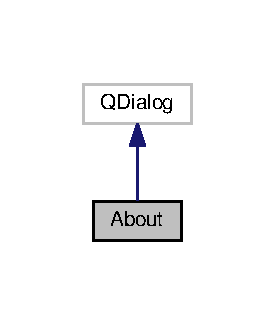
\includegraphics[width=132pt]{class_about__inherit__graph}
\end{center}
\end{figure}


Collaboration diagram for About\+:
\nopagebreak
\begin{figure}[H]
\begin{center}
\leavevmode
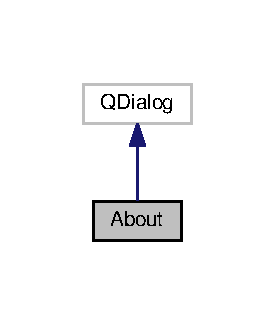
\includegraphics[width=132pt]{class_about__coll__graph}
\end{center}
\end{figure}
\subsubsection*{Public Member Functions}
\begin{DoxyCompactItemize}
\item 
\hyperlink{group___window_gab79599ebbcdeffe0a96e00f010e64177}{About} (Q\+Widget $\ast$parent=0)
\begin{DoxyCompactList}\small\item\em Constructor. \end{DoxyCompactList}\item 
\hyperlink{group___window_gace60197b1b610998908036ee1f802204}{$\sim$\+About} ()
\begin{DoxyCompactList}\small\item\em Destructor. \end{DoxyCompactList}\end{DoxyCompactItemize}


\subsubsection{Detailed Description}
\subparagraph*{Overview}

Contains information about the author and the software. Should be linked to an action (about action).

\subparagraph*{Example}


\begin{DoxyCode}
\textcolor{comment}{// Just invoke the exec somewhere in your code.}
\hyperlink{class_about}{About} about(\textcolor{keyword}{this});
about.exec();
\end{DoxyCode}
 

Definition at line \hyperlink{about_8h_source_l00068}{68} of file \hyperlink{about_8h_source}{about.\+h}.



The documentation for this class was generated from the following files\+:\begin{DoxyCompactItemize}
\item 
\hyperlink{about_8h}{about.\+h}\item 
\hyperlink{about_8cpp}{about.\+cpp}\end{DoxyCompactItemize}

\hypertarget{class_bar}{}\subsection{Bar Class Reference}
\label{class_bar}\index{Bar@{Bar}}


Represents a busbar in power distribution systems.  




Inheritance diagram for Bar\+:\nopagebreak
\begin{figure}[H]
\begin{center}
\leavevmode
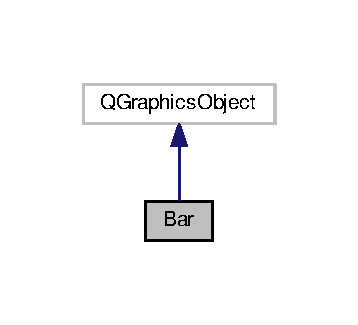
\includegraphics[width=172pt]{class_bar__inherit__graph}
\end{center}
\end{figure}


Collaboration diagram for Bar\+:\nopagebreak
\begin{figure}[H]
\begin{center}
\leavevmode
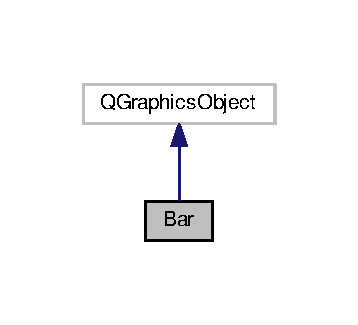
\includegraphics[width=244pt]{class_bar__coll__graph}
\end{center}
\end{figure}
\subsubsection*{Signals}
\begin{DoxyCompactItemize}
\item 
void \hyperlink{class_bar_a66bcbd19582dddee7e171ae5a4475f4b}{event\+Double\+Click} ()
\begin{DoxyCompactList}\small\item\em Double click signal. \end{DoxyCompactList}\end{DoxyCompactItemize}
\subsubsection*{Public Member Functions}
\begin{DoxyCompactItemize}
\item 
\hyperlink{group___models_ga9cae2188fcc6cce41caa7898c64548d1}{Bar} ()
\begin{DoxyCompactList}\small\item\em Constructor. \end{DoxyCompactList}\item 
\hyperlink{group___models_gab1c5a81ad40dbc7ee745077b4f5c20d4}{Bar} (complex$<$ double $>$ initial\+V, complex$<$ double $>$ initial\+Sh=0.\+0, complex$<$ double $>$ initial\+Si=0.\+0)
\begin{DoxyCompactList}\small\item\em Constructor. \end{DoxyCompactList}\item 
virtual \hyperlink{group___models_ga9c7ebea0c189423591741ac438985316}{$\sim$\+Bar} ()
\begin{DoxyCompactList}\small\item\em Destructor. \end{DoxyCompactList}\item 
complex$<$ double $>$ \hyperlink{group___models_ga1e6f2daec86407118656d88170d1adc2}{v} (int32\+\_\+t phase, \hyperlink{class_unit_a55b07dfa9457e1eca2c7194fe0cfc3c1}{Unit\+::\+Voltage\+Unit} unit=\hyperlink{class_unit_a55b07dfa9457e1eca2c7194fe0cfc3c1aa54b2473993a702a3923525765bd6e4c}{Unit\+::k\+Volts})
\begin{DoxyCompactList}\small\item\em Initial Voltage. \end{DoxyCompactList}\item 
void \hyperlink{group___models_ga9b6fbc92674bfcdc9d5090795ab335a6}{set\+V} (int32\+\_\+t phase, complex$<$ double $>$ new\+Voltage, \hyperlink{class_unit_a55b07dfa9457e1eca2c7194fe0cfc3c1}{Unit\+::\+Voltage\+Unit} unit=\hyperlink{class_unit_a55b07dfa9457e1eca2c7194fe0cfc3c1aa54b2473993a702a3923525765bd6e4c}{Unit\+::k\+Volts})
\begin{DoxyCompactList}\small\item\em Set initial voltage. \end{DoxyCompactList}\item 
complex$<$ double $>$ \hyperlink{group___models_gac188071bf5f165b0acdaa4c8af82355c}{sh} (int32\+\_\+t phase, \hyperlink{class_unit_ace265ae255370ccacfd5370337572c3b}{Unit\+::\+Power\+Unit} unit=\hyperlink{class_unit_ace265ae255370ccacfd5370337572c3ba72b181a842ae2759488a2fa1410d3696}{Unit\+::k\+V\+A})
\begin{DoxyCompactList}\small\item\em Shutn element. \end{DoxyCompactList}\item 
void \hyperlink{group___models_ga207abd3d0649a488e3c44cf2a501ed23}{set\+Sh} (int32\+\_\+t phase, complex$<$ double $>$ new\+Power, \hyperlink{class_unit_ace265ae255370ccacfd5370337572c3b}{Unit\+::\+Power\+Unit} unit=\hyperlink{class_unit_ace265ae255370ccacfd5370337572c3ba72b181a842ae2759488a2fa1410d3696}{Unit\+::k\+V\+A})
\begin{DoxyCompactList}\small\item\em Set Shunt power. \end{DoxyCompactList}\item 
complex$<$ double $>$ \hyperlink{group___models_ga02bbc279f1e133f66b12ee21e7bebcd8}{si} (int32\+\_\+t phase, \hyperlink{class_unit_ace265ae255370ccacfd5370337572c3b}{Unit\+::\+Power\+Unit} unit=\hyperlink{class_unit_ace265ae255370ccacfd5370337572c3ba72b181a842ae2759488a2fa1410d3696}{Unit\+::k\+V\+A})
\begin{DoxyCompactList}\small\item\em Injected power. \end{DoxyCompactList}\item 
void \hyperlink{group___models_ga74e510be49e50e4c14550b32e1dc92f9}{set\+Si} (int32\+\_\+t phase, complex$<$ double $>$ new\+Power, \hyperlink{class_unit_ace265ae255370ccacfd5370337572c3b}{Unit\+::\+Power\+Unit} unit=\hyperlink{class_unit_ace265ae255370ccacfd5370337572c3ba72b181a842ae2759488a2fa1410d3696}{Unit\+::k\+V\+A})
\begin{DoxyCompactList}\small\item\em Set the injected power. \end{DoxyCompactList}\item 
complex$<$ double $>$ \hyperlink{group___models_ga2d1f6bfbd8abaf168bb75bd8e5cd9b5e}{r\+V} (int32\+\_\+t phase, \hyperlink{class_unit_a55b07dfa9457e1eca2c7194fe0cfc3c1}{Unit\+::\+Voltage\+Unit} unit=\hyperlink{class_unit_a55b07dfa9457e1eca2c7194fe0cfc3c1aa54b2473993a702a3923525765bd6e4c}{Unit\+::k\+Volts})
\begin{DoxyCompactList}\small\item\em Result bar voltage. \end{DoxyCompactList}\item 
void \hyperlink{group___models_ga2b2c5a373d87025e79d26aa9c4cea75a}{set\+R\+V} (int32\+\_\+t phase, complex$<$ double $>$ result\+Voltage, \hyperlink{class_unit_a55b07dfa9457e1eca2c7194fe0cfc3c1}{Unit\+::\+Voltage\+Unit} unit=\hyperlink{class_unit_a55b07dfa9457e1eca2c7194fe0cfc3c1aa54b2473993a702a3923525765bd6e4c}{Unit\+::k\+Volts})
\begin{DoxyCompactList}\small\item\em Set result voltage. \end{DoxyCompactList}\item 
complex$<$ double $>$ \hyperlink{group___models_ga8a009531f01430aa68eba739bb0dc2ea}{r\+I} (int32\+\_\+t phase, \hyperlink{class_unit_a0794cf6c9682f48296dd4a5315389787}{Unit\+::\+Current\+Unit} unit=\hyperlink{class_unit_a0794cf6c9682f48296dd4a5315389787a368a3c470f0b590a6100dda717a7dd4f}{Unit\+::k\+Ampere})
\begin{DoxyCompactList}\small\item\em Result bar current. \end{DoxyCompactList}\item 
void \hyperlink{group___models_ga8cbd2f62d92e69ce6c8d561b682464b6}{add\+Line} (\hyperlink{class_line}{Line} $\ast$line)
\begin{DoxyCompactList}\small\item\em Add line to bar. \end{DoxyCompactList}\item 
void \hyperlink{group___models_ga2536c0e5cb97fb627b3520826ece2c99}{remove\+Line} (\hyperlink{class_line}{Line} $\ast$line)
\begin{DoxyCompactList}\small\item\em Remove line link;. \end{DoxyCompactList}\item 
void \hyperlink{group___models_ga4ea1a2074cb45968d80d6add571884a4}{remove\+Lines} ()
\begin{DoxyCompactList}\small\item\em Remove all lines from this bar. \end{DoxyCompactList}\item 
Q\+Json\+Object \hyperlink{group___models_ga3eb84c42b687db6cd98e11b8bd38c86e}{to\+Json} ()
\begin{DoxyCompactList}\small\item\em Convert bar data to json object. \end{DoxyCompactList}\item 
void \hyperlink{group___models_ga1df62f03dd3a066ceaf6588ba6bb6004}{from\+Json} (Q\+Json\+Object \&json\+Bar)
\begin{DoxyCompactList}\small\item\em Fill bar data from Json data. \end{DoxyCompactList}\item 
Q\+Rect\+F \hyperlink{group___models_ga8279d8109019cc7e139e2023690496be}{bounding\+Rect} () const Q\+\_\+\+D\+E\+C\+L\+\_\+\+O\+V\+E\+R\+R\+I\+D\+E
\begin{DoxyCompactList}\small\item\em \hyperlink{class_bar}{Bar} bounding rect. \end{DoxyCompactList}\end{DoxyCompactItemize}
\subsubsection*{Public Attributes}
\begin{DoxyCompactItemize}
\item 
int32\+\_\+t \hyperlink{class_bar_a9dc5c6a6d44fe412ae34ef8a881b8dce}{id}
\begin{DoxyCompactList}\small\item\em The bar id. \end{DoxyCompactList}\item 
\hyperlink{class_network}{Network} $\ast$ \hyperlink{class_bar_a80025f13884750add58cc61b318357ff}{network}
\begin{DoxyCompactList}\small\item\em A reference to the \hyperlink{class_network}{Network} where the bar is. \end{DoxyCompactList}\item 
Q\+Vector$<$ \hyperlink{class_line}{Line} $\ast$ $>$ \hyperlink{class_bar_a23b6d4319352ef0e77ad66aade4e0209}{lines}
\begin{DoxyCompactList}\small\item\em Lines connected to this bar. \end{DoxyCompactList}\end{DoxyCompactItemize}
\subsubsection*{Static Public Attributes}
\begin{DoxyCompactItemize}
\item 
static const int32\+\_\+t \hyperlink{group___models_ga9919592c0397ed41448dfb20b607d738}{k\+Invalid\+Id} = -\/1
\begin{DoxyCompactList}\small\item\em Indicates an invalid bar. \end{DoxyCompactList}\end{DoxyCompactItemize}
\subsubsection*{Protected Member Functions}
\begin{DoxyCompactItemize}
\item 
void \hyperlink{group___models_ga1945e7b4401fa9ad7475274d9fb12a72}{mouse\+Double\+Click\+Event} (Q\+Graphics\+Scene\+Mouse\+Event $\ast$event)
\begin{DoxyCompactList}\small\item\em Mouse double click event. \end{DoxyCompactList}\item 
Q\+Variant \hyperlink{group___models_gad97a82d618ee0c51a9a36e44339c69e6}{item\+Change} (Graphics\+Item\+Change change, const Q\+Variant \&value) Q\+\_\+\+D\+E\+C\+L\+\_\+\+O\+V\+E\+R\+R\+I\+D\+E
\begin{DoxyCompactList}\small\item\em Item change. \end{DoxyCompactList}\item 
void \hyperlink{group___models_gacbb6dbac607412c9c1f9dfcd0cd4d432}{paint} (Q\+Painter $\ast$painter, const Q\+Style\+Option\+Graphics\+Item $\ast$option, Q\+Widget $\ast$widget) Q\+\_\+\+D\+E\+C\+L\+\_\+\+O\+V\+E\+R\+R\+I\+D\+E
\begin{DoxyCompactList}\small\item\em \hyperlink{class_bar}{Bar} paint function. \end{DoxyCompactList}\end{DoxyCompactItemize}


\subsubsection{Detailed Description}
\subparagraph*{Overview}

\hyperlink{class_bar}{Bar} class represents a bar in a power system, providing the data structure and methods that model a real bar. The class also provides the graphical structure to be displayed in a Syste\+View widget. A bar with id equals to 0 is an alimentator (Slack bar). \hyperlink{class_bar}{Bar} properties are\+:
\begin{DoxyItemize}
\item Voltage (for phases 0, 1 and 2)\+: voltage at the bar.
\item Shunt elements (sh) power injection\+: shunt elements are represented by the power they inject in the bar.
\item Injected power (si)\+: the power injected at the bar (here, power that is consumed is represented as a positive value and power that is generated at the bar is represented with a negative sign).
\end{DoxyItemize}

The bar properties are stored in the following units\+:
\begin{DoxyItemize}
\item Power\+: V\+A.
\item Voltage\+: Volts.
\end{DoxyItemize}

In order to use diferent units, use the option parameter {\bfseries unit} with the desired unit.

Bars must be added to a network in order to be displayed by a \hyperlink{class_system_view}{System\+View}.

\#\#\# Example 
\begin{DoxyCode}
\textcolor{comment}{// Code to add a bar.}

\textcolor{comment}{// External objects where the bar will be put in.}
\textcolor{keyword}{extern} \hyperlink{class_system_view}{SystemView} systemView;
\textcolor{keyword}{extern} SystemScene systemScene;
\textcolor{keyword}{extern} \hyperlink{class_network}{Network} \hyperlink{class_bar_a80025f13884750add58cc61b318357ff}{network};

\hyperlink{class_bar}{Bar} * bar = \textcolor{keyword}{new} \hyperlink{group___models_ga9cae2188fcc6cce41caa7898c64548d1}{Bar};
\textcolor{comment}{// Bar id must be defined.}
\hyperlink{class_bar}{Bar}->\hyperlink{class_bar_a9dc5c6a6d44fe412ae34ef8a881b8dce}{id} = 20;

network.\hyperlink{group___graphics_ga8c5dfef0216731246f7411e1a5fbee01}{addBar}(bar);
systemScene addNetwork(&network);
systemView.addScene(&systemScene);
\end{DoxyCode}


\begin{DoxyNote}{Note}
The values v, sh and si are the initial conditions. Results of the load flow calculation have a \char`\"{}r\char`\"{} in the name, like r\+V and r\+Si. 
\end{DoxyNote}


Definition at line \hyperlink{bar_8h_source_l00112}{112} of file \hyperlink{bar_8h_source}{bar.\+h}.



\subsubsection{Member Function Documentation}
\hypertarget{class_bar_a66bcbd19582dddee7e171ae5a4475f4b}{}\index{Bar@{Bar}!event\+Double\+Click@{event\+Double\+Click}}
\index{event\+Double\+Click@{event\+Double\+Click}!Bar@{Bar}}
\paragraph[{event\+Double\+Click}]{\setlength{\rightskip}{0pt plus 5cm}void Bar\+::event\+Double\+Click (
\begin{DoxyParamCaption}
{}
\end{DoxyParamCaption}
)\hspace{0.3cm}{\ttfamily [signal]}}\label{class_bar_a66bcbd19582dddee7e171ae5a4475f4b}
Signal emited when a double click occurs. 

Here is the caller graph for this function\+:\nopagebreak
\begin{figure}[H]
\begin{center}
\leavevmode
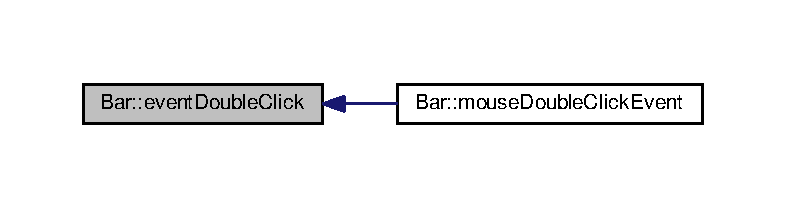
\includegraphics[width=350pt]{class_bar_a66bcbd19582dddee7e171ae5a4475f4b_icgraph}
\end{center}
\end{figure}




\subsubsection{Member Data Documentation}
\hypertarget{class_bar_a9dc5c6a6d44fe412ae34ef8a881b8dce}{}\index{Bar@{Bar}!id@{id}}
\index{id@{id}!Bar@{Bar}}
\paragraph[{id}]{\setlength{\rightskip}{0pt plus 5cm}int32\+\_\+t Bar\+::id}\label{class_bar_a9dc5c6a6d44fe412ae34ef8a881b8dce}
Id number if the bar. A bar with I\+D 0 will be the slack bar. Only one bar in a network can be a slack and every other bars need an id $>$ 0. 

Definition at line \hyperlink{bar_8h_source_l00137}{137} of file \hyperlink{bar_8h_source}{bar.\+h}.

\hypertarget{class_bar_a23b6d4319352ef0e77ad66aade4e0209}{}\index{Bar@{Bar}!lines@{lines}}
\index{lines@{lines}!Bar@{Bar}}
\paragraph[{lines}]{\setlength{\rightskip}{0pt plus 5cm}Q\+Vector$<${\bf Line} $\ast$$>$ Bar\+::lines}\label{class_bar_a23b6d4319352ef0e77ad66aade4e0209}
All lines that connect to this bar are listed here. \begin{DoxyWarning}{Warning}
Don\textquotesingle{}t use the lines vector to manipulate lines directly. Instead, use the provided add and remove functions. 
\end{DoxyWarning}


Definition at line \hyperlink{bar_8h_source_l00152}{152} of file \hyperlink{bar_8h_source}{bar.\+h}.

\hypertarget{class_bar_a80025f13884750add58cc61b318357ff}{}\index{Bar@{Bar}!network@{network}}
\index{network@{network}!Bar@{Bar}}
\paragraph[{network}]{\setlength{\rightskip}{0pt plus 5cm}{\bf Network}$\ast$ Bar\+::network}\label{class_bar_a80025f13884750add58cc61b318357ff}
This option is used internaly to determine color settings and units. \begin{DoxyWarning}{Warning}
This option must be not N\+U\+L\+L in order to add the bar to a scene. 
\end{DoxyWarning}


Definition at line \hyperlink{bar_8h_source_l00144}{144} of file \hyperlink{bar_8h_source}{bar.\+h}.



The documentation for this class was generated from the following files\+:\begin{DoxyCompactItemize}
\item 
\hyperlink{bar_8h}{bar.\+h}\item 
\hyperlink{bar_8cpp}{bar.\+cpp}\end{DoxyCompactItemize}

\hypertarget{class_bar_properties}{}\subsection{Bar\+Properties Class Reference}
\label{class_bar_properties}\index{Bar\+Properties@{Bar\+Properties}}


Inheritance diagram for Bar\+Properties\+:\nopagebreak
\begin{figure}[H]
\begin{center}
\leavevmode
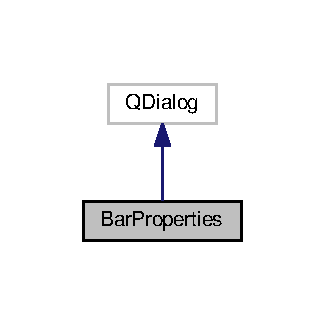
\includegraphics[width=156pt]{class_bar_properties__inherit__graph}
\end{center}
\end{figure}


Collaboration diagram for Bar\+Properties\+:\nopagebreak
\begin{figure}[H]
\begin{center}
\leavevmode
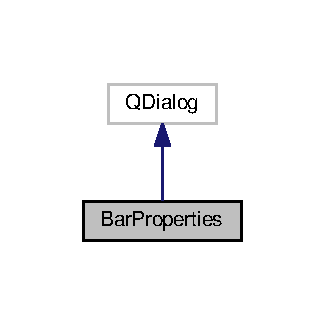
\includegraphics[width=156pt]{class_bar_properties__coll__graph}
\end{center}
\end{figure}
\subsubsection*{Public Member Functions}
\begin{DoxyCompactItemize}
\item 
\hyperlink{class_bar_properties_a7c14a54f430cabfe872869799076025b}{Bar\+Properties} (Q\+Widget $\ast$parent=0)
\item 
\hyperlink{class_bar_properties_a639b4da849970025a2935ee965d6a465}{$\sim$\+Bar\+Properties} ()
\item 
void \hyperlink{class_bar_properties_a80cba99404820272603c4da8fb708c05}{set\+Options} (\hyperlink{class_project}{Project} $\ast$project, \hyperlink{class_bar}{Bar} $\ast$\hyperlink{class_bar_properties_a65d09e7315764cd4ad33b5a0ded32090}{bar})
\item 
\hyperlink{class_bar}{Bar} $\ast$ \hyperlink{class_bar_properties_a65d09e7315764cd4ad33b5a0ded32090}{bar} ()
\end{DoxyCompactItemize}


\subsubsection{Detailed Description}


Definition at line \hyperlink{barproperties_8h_source_l00013}{13} of file \hyperlink{barproperties_8h_source}{barproperties.\+h}.



\subsubsection{Constructor \& Destructor Documentation}
\hypertarget{class_bar_properties_a7c14a54f430cabfe872869799076025b}{}\index{Bar\+Properties@{Bar\+Properties}!Bar\+Properties@{Bar\+Properties}}
\index{Bar\+Properties@{Bar\+Properties}!Bar\+Properties@{Bar\+Properties}}
\paragraph[{Bar\+Properties}]{\setlength{\rightskip}{0pt plus 5cm}Bar\+Properties\+::\+Bar\+Properties (
\begin{DoxyParamCaption}
\item[{Q\+Widget $\ast$}]{parent = {\ttfamily 0}}
\end{DoxyParamCaption}
)\hspace{0.3cm}{\ttfamily [explicit]}}\label{class_bar_properties_a7c14a54f430cabfe872869799076025b}


Definition at line \hyperlink{barproperties_8cpp_source_l00009}{9} of file \hyperlink{barproperties_8cpp_source}{barproperties.\+cpp}.

\hypertarget{class_bar_properties_a639b4da849970025a2935ee965d6a465}{}\index{Bar\+Properties@{Bar\+Properties}!````~Bar\+Properties@{$\sim$\+Bar\+Properties}}
\index{````~Bar\+Properties@{$\sim$\+Bar\+Properties}!Bar\+Properties@{Bar\+Properties}}
\paragraph[{$\sim$\+Bar\+Properties}]{\setlength{\rightskip}{0pt plus 5cm}Bar\+Properties\+::$\sim$\+Bar\+Properties (
\begin{DoxyParamCaption}
{}
\end{DoxyParamCaption}
)}\label{class_bar_properties_a639b4da849970025a2935ee965d6a465}


Definition at line \hyperlink{barproperties_8cpp_source_l00044}{44} of file \hyperlink{barproperties_8cpp_source}{barproperties.\+cpp}.



\subsubsection{Member Function Documentation}
\hypertarget{class_bar_properties_a65d09e7315764cd4ad33b5a0ded32090}{}\index{Bar\+Properties@{Bar\+Properties}!bar@{bar}}
\index{bar@{bar}!Bar\+Properties@{Bar\+Properties}}
\paragraph[{bar}]{\setlength{\rightskip}{0pt plus 5cm}{\bf Bar} $\ast$ Bar\+Properties\+::bar (
\begin{DoxyParamCaption}
{}
\end{DoxyParamCaption}
)}\label{class_bar_properties_a65d09e7315764cd4ad33b5a0ded32090}


Definition at line \hyperlink{barproperties_8cpp_source_l00124}{124} of file \hyperlink{barproperties_8cpp_source}{barproperties.\+cpp}.



Here is the caller graph for this function\+:\nopagebreak
\begin{figure}[H]
\begin{center}
\leavevmode
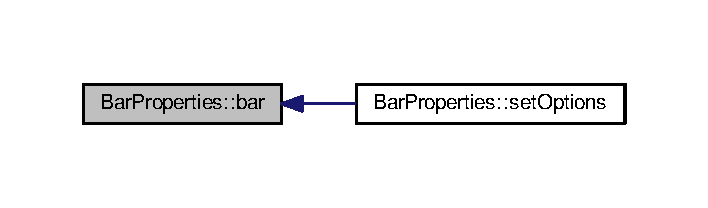
\includegraphics[width=340pt]{class_bar_properties_a65d09e7315764cd4ad33b5a0ded32090_icgraph}
\end{center}
\end{figure}


\hypertarget{class_bar_properties_a80cba99404820272603c4da8fb708c05}{}\index{Bar\+Properties@{Bar\+Properties}!set\+Options@{set\+Options}}
\index{set\+Options@{set\+Options}!Bar\+Properties@{Bar\+Properties}}
\paragraph[{set\+Options}]{\setlength{\rightskip}{0pt plus 5cm}void Bar\+Properties\+::set\+Options (
\begin{DoxyParamCaption}
\item[{{\bf Project} $\ast$}]{project, }
\item[{{\bf Bar} $\ast$}]{bar}
\end{DoxyParamCaption}
)}\label{class_bar_properties_a80cba99404820272603c4da8fb708c05}


Definition at line \hyperlink{barproperties_8cpp_source_l00052}{52} of file \hyperlink{barproperties_8cpp_source}{barproperties.\+cpp}.



Here is the call graph for this function\+:\nopagebreak
\begin{figure}[H]
\begin{center}
\leavevmode
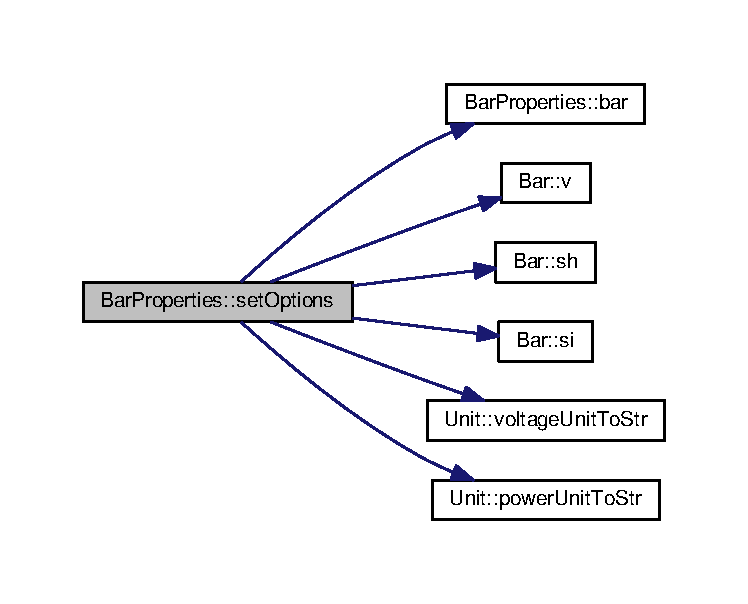
\includegraphics[width=350pt]{class_bar_properties_a80cba99404820272603c4da8fb708c05_cgraph}
\end{center}
\end{figure}




The documentation for this class was generated from the following files\+:\begin{DoxyCompactItemize}
\item 
\hyperlink{barproperties_8h}{barproperties.\+h}\item 
\hyperlink{barproperties_8cpp}{barproperties.\+cpp}\end{DoxyCompactItemize}

\hypertarget{class_cespedes}{}\subsection{Cespedes Class Reference}
\label{class_cespedes}\index{Cespedes@{Cespedes}}
\subsubsection*{Public Member Functions}
\begin{DoxyCompactItemize}
\item 
\hyperlink{class_cespedes_a99ce54693c7ff065d8973167cee9caa7}{Cespedes} ()
\end{DoxyCompactItemize}


\subsubsection{Detailed Description}


Definition at line \hyperlink{cespedes_8h_source_l00005}{5} of file \hyperlink{cespedes_8h_source}{cespedes.\+h}.



\subsubsection{Constructor \& Destructor Documentation}
\hypertarget{class_cespedes_a99ce54693c7ff065d8973167cee9caa7}{}\index{Cespedes@{Cespedes}!Cespedes@{Cespedes}}
\index{Cespedes@{Cespedes}!Cespedes@{Cespedes}}
\paragraph[{Cespedes}]{\setlength{\rightskip}{0pt plus 5cm}Cespedes\+::\+Cespedes (
\begin{DoxyParamCaption}
{}
\end{DoxyParamCaption}
)}\label{class_cespedes_a99ce54693c7ff065d8973167cee9caa7}


Definition at line \hyperlink{cespedes_8cpp_source_l00003}{3} of file \hyperlink{cespedes_8cpp_source}{cespedes.\+cpp}.



The documentation for this class was generated from the following files\+:\begin{DoxyCompactItemize}
\item 
\hyperlink{cespedes_8h}{cespedes.\+h}\item 
\hyperlink{cespedes_8cpp}{cespedes.\+cpp}\end{DoxyCompactItemize}

\hypertarget{class_data_table}{}\subsection{Data\+Table Class Reference}
\label{class_data_table}\index{Data\+Table@{Data\+Table}}
\subsubsection*{Public Member Functions}
\begin{DoxyCompactItemize}
\item 
\hyperlink{class_data_table_a9d37b5de498e8436f74cd51e51ec4948}{Data\+Table} (int32\+\_\+t rows, int32\+\_\+t colums)
\item 
\hyperlink{class_data_table_a86095a8a5abd63d50603d4ca0db253d7}{$\sim$\+Data\+Table} ()
\item 
void \hyperlink{class_data_table_a8a8cd6f95caaaff148993f8e28eeb703}{set\+Size} (Q\+Rect\+F \&size)
\item 
void \hyperlink{class_data_table_aee0d28c77116b51360f0124a529cb3ff}{set\+Text} (Q\+String \&text, int32\+\_\+t row, int32\+\_\+t col)
\item 
void \hyperlink{class_data_table_a3a3695e88dcd4d4aad5cc941ec7e6e55}{draw\+Table} (Q\+Painter $\ast$painter)
\end{DoxyCompactItemize}
\subsubsection*{Static Public Attributes}
\begin{DoxyCompactItemize}
\item 
static const double \hyperlink{class_data_table_aa4aed4c624ca9a8e68c9ecc4d2b43458}{k\+Table\+Line\+Width} = 1.\+0
\item 
static const double \hyperlink{class_data_table_ab0703eeee2cf6e45fc74356432434ac6}{k\+Text\+To\+Line\+Pad} = 1.\+0
\end{DoxyCompactItemize}


\subsubsection{Detailed Description}


Definition at line \hyperlink{datatable_8h_source_l00009}{9} of file \hyperlink{datatable_8h_source}{datatable.\+h}.



\subsubsection{Constructor \& Destructor Documentation}
\hypertarget{class_data_table_a9d37b5de498e8436f74cd51e51ec4948}{}\index{Data\+Table@{Data\+Table}!Data\+Table@{Data\+Table}}
\index{Data\+Table@{Data\+Table}!Data\+Table@{Data\+Table}}
\paragraph[{Data\+Table}]{\setlength{\rightskip}{0pt plus 5cm}Data\+Table\+::\+Data\+Table (
\begin{DoxyParamCaption}
\item[{int32\+\_\+t}]{rows, }
\item[{int32\+\_\+t}]{colums}
\end{DoxyParamCaption}
)}\label{class_data_table_a9d37b5de498e8436f74cd51e51ec4948}


Definition at line \hyperlink{datatable_8cpp_source_l00007}{7} of file \hyperlink{datatable_8cpp_source}{datatable.\+cpp}.

\hypertarget{class_data_table_a86095a8a5abd63d50603d4ca0db253d7}{}\index{Data\+Table@{Data\+Table}!````~Data\+Table@{$\sim$\+Data\+Table}}
\index{````~Data\+Table@{$\sim$\+Data\+Table}!Data\+Table@{Data\+Table}}
\paragraph[{$\sim$\+Data\+Table}]{\setlength{\rightskip}{0pt plus 5cm}Data\+Table\+::$\sim$\+Data\+Table (
\begin{DoxyParamCaption}
{}
\end{DoxyParamCaption}
)}\label{class_data_table_a86095a8a5abd63d50603d4ca0db253d7}


Definition at line \hyperlink{datatable_8cpp_source_l00014}{14} of file \hyperlink{datatable_8cpp_source}{datatable.\+cpp}.



\subsubsection{Member Function Documentation}
\hypertarget{class_data_table_a3a3695e88dcd4d4aad5cc941ec7e6e55}{}\index{Data\+Table@{Data\+Table}!draw\+Table@{draw\+Table}}
\index{draw\+Table@{draw\+Table}!Data\+Table@{Data\+Table}}
\paragraph[{draw\+Table}]{\setlength{\rightskip}{0pt plus 5cm}void Data\+Table\+::draw\+Table (
\begin{DoxyParamCaption}
\item[{Q\+Painter $\ast$}]{painter}
\end{DoxyParamCaption}
)}\label{class_data_table_a3a3695e88dcd4d4aad5cc941ec7e6e55}


Definition at line \hyperlink{datatable_8cpp_source_l00029}{29} of file \hyperlink{datatable_8cpp_source}{datatable.\+cpp}.



Here is the caller graph for this function\+:
\nopagebreak
\begin{figure}[H]
\begin{center}
\leavevmode
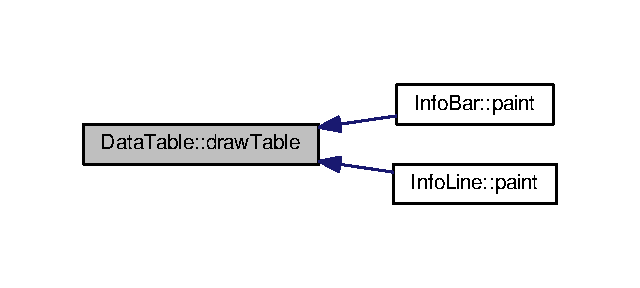
\includegraphics[width=307pt]{class_data_table_a3a3695e88dcd4d4aad5cc941ec7e6e55_icgraph}
\end{center}
\end{figure}


\hypertarget{class_data_table_a8a8cd6f95caaaff148993f8e28eeb703}{}\index{Data\+Table@{Data\+Table}!set\+Size@{set\+Size}}
\index{set\+Size@{set\+Size}!Data\+Table@{Data\+Table}}
\paragraph[{set\+Size}]{\setlength{\rightskip}{0pt plus 5cm}void Data\+Table\+::set\+Size (
\begin{DoxyParamCaption}
\item[{Q\+Rect\+F \&}]{size}
\end{DoxyParamCaption}
)}\label{class_data_table_a8a8cd6f95caaaff148993f8e28eeb703}


Definition at line \hyperlink{datatable_8cpp_source_l00019}{19} of file \hyperlink{datatable_8cpp_source}{datatable.\+cpp}.



Here is the caller graph for this function\+:
\nopagebreak
\begin{figure}[H]
\begin{center}
\leavevmode
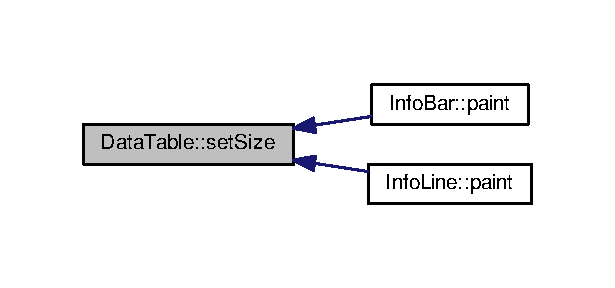
\includegraphics[width=295pt]{class_data_table_a8a8cd6f95caaaff148993f8e28eeb703_icgraph}
\end{center}
\end{figure}


\hypertarget{class_data_table_aee0d28c77116b51360f0124a529cb3ff}{}\index{Data\+Table@{Data\+Table}!set\+Text@{set\+Text}}
\index{set\+Text@{set\+Text}!Data\+Table@{Data\+Table}}
\paragraph[{set\+Text}]{\setlength{\rightskip}{0pt plus 5cm}void Data\+Table\+::set\+Text (
\begin{DoxyParamCaption}
\item[{Q\+String \&}]{text, }
\item[{int32\+\_\+t}]{row, }
\item[{int32\+\_\+t}]{col}
\end{DoxyParamCaption}
)}\label{class_data_table_aee0d28c77116b51360f0124a529cb3ff}


Definition at line \hyperlink{datatable_8cpp_source_l00024}{24} of file \hyperlink{datatable_8cpp_source}{datatable.\+cpp}.



Here is the caller graph for this function\+:
\nopagebreak
\begin{figure}[H]
\begin{center}
\leavevmode
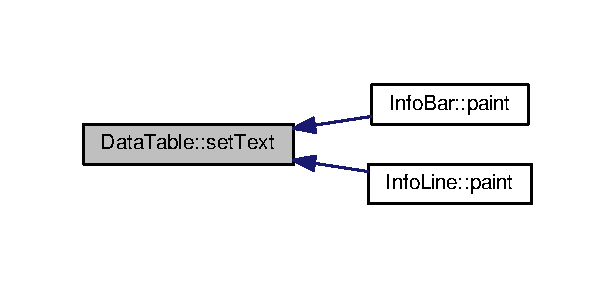
\includegraphics[width=295pt]{class_data_table_aee0d28c77116b51360f0124a529cb3ff_icgraph}
\end{center}
\end{figure}




\subsubsection{Member Data Documentation}
\hypertarget{class_data_table_aa4aed4c624ca9a8e68c9ecc4d2b43458}{}\index{Data\+Table@{Data\+Table}!k\+Table\+Line\+Width@{k\+Table\+Line\+Width}}
\index{k\+Table\+Line\+Width@{k\+Table\+Line\+Width}!Data\+Table@{Data\+Table}}
\paragraph[{k\+Table\+Line\+Width}]{\setlength{\rightskip}{0pt plus 5cm}const double Data\+Table\+::k\+Table\+Line\+Width = 1.\+0\hspace{0.3cm}{\ttfamily [static]}}\label{class_data_table_aa4aed4c624ca9a8e68c9ecc4d2b43458}


Definition at line \hyperlink{datatable_8h_source_l00014}{14} of file \hyperlink{datatable_8h_source}{datatable.\+h}.

\hypertarget{class_data_table_ab0703eeee2cf6e45fc74356432434ac6}{}\index{Data\+Table@{Data\+Table}!k\+Text\+To\+Line\+Pad@{k\+Text\+To\+Line\+Pad}}
\index{k\+Text\+To\+Line\+Pad@{k\+Text\+To\+Line\+Pad}!Data\+Table@{Data\+Table}}
\paragraph[{k\+Text\+To\+Line\+Pad}]{\setlength{\rightskip}{0pt plus 5cm}const double Data\+Table\+::k\+Text\+To\+Line\+Pad = 1.\+0\hspace{0.3cm}{\ttfamily [static]}}\label{class_data_table_ab0703eeee2cf6e45fc74356432434ac6}


Definition at line \hyperlink{datatable_8h_source_l00015}{15} of file \hyperlink{datatable_8h_source}{datatable.\+h}.



The documentation for this class was generated from the following files\+:\begin{DoxyCompactItemize}
\item 
\hyperlink{datatable_8h}{datatable.\+h}\item 
\hyperlink{datatable_8cpp}{datatable.\+cpp}\end{DoxyCompactItemize}

\hypertarget{class_info_bar}{}\subsection{Info\+Bar Class Reference}
\label{class_info_bar}\index{Info\+Bar@{Info\+Bar}}


Inheritance diagram for Info\+Bar\+:
\nopagebreak
\begin{figure}[H]
\begin{center}
\leavevmode
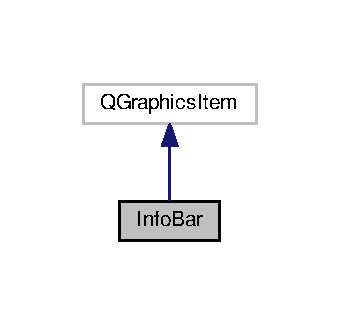
\includegraphics[width=163pt]{class_info_bar__inherit__graph}
\end{center}
\end{figure}


Collaboration diagram for Info\+Bar\+:
\nopagebreak
\begin{figure}[H]
\begin{center}
\leavevmode
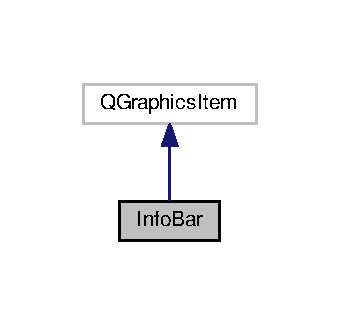
\includegraphics[width=163pt]{class_info_bar__coll__graph}
\end{center}
\end{figure}
\subsubsection*{Public Member Functions}
\begin{DoxyCompactItemize}
\item 
\hyperlink{class_info_bar_aab5c08f226901c8827a97efbdfb5122a}{Info\+Bar} (\hyperlink{class_bar}{Bar} $\ast$bar)
\item 
\hyperlink{class_info_bar_a954baa28d750739c80c029818d267d8e}{$\sim$\+Info\+Bar} ()
\item 
Q\+Rect\+F \hyperlink{class_info_bar_a564aacb3b64bdb5fbcaef8a432a0b49e}{bounding\+Rect} () const Q\+\_\+\+D\+E\+C\+L\+\_\+\+O\+V\+E\+R\+R\+I\+D\+E
\end{DoxyCompactItemize}
\subsubsection*{Static Public Attributes}
\begin{DoxyCompactItemize}
\item 
static const int \hyperlink{class_info_bar_ad54d2dd19a63caf9d2476aace60ae3c5}{k\+Table\+Rows} = 4
\item 
static const int \hyperlink{class_info_bar_a57e9e7c40a6fd2a56dd47a4512d65489}{k\+Table\+Colums} = 3
\item 
static const qreal \hyperlink{class_info_bar_aa1c35ddbae0324743d90721037447571}{k\+Box\+Width} = 135.\+0$\ast$\hyperlink{class_info_bar_a57e9e7c40a6fd2a56dd47a4512d65489}{k\+Table\+Colums}
\item 
static const qreal \hyperlink{class_info_bar_aba381a3838a5e064f1372f2f2b4d8e0d}{k\+Box\+Height} = 37.\+5$\ast$\hyperlink{class_info_bar_ad54d2dd19a63caf9d2476aace60ae3c5}{k\+Table\+Rows}
\item 
static const qreal \hyperlink{class_info_bar_a46d929f42476a6ad37422adee1783712}{k\+Line\+Width} = 2.\+0
\item 
static const qreal \hyperlink{class_info_bar_ae24b5cac460550a4c86203a3dbd96ba9}{k\+Margin\+Head\+Top} = 5.\+0
\item 
static const qreal \hyperlink{class_info_bar_a0cfbafbc9f780fc1366157b9c8379463}{k\+Margin\+Head\+Bot} = 5.\+0
\item 
static const qreal \hyperlink{class_info_bar_add145842c6a2331a7edf9e5be301e5b4}{k\+Margin\+Top} = 5.\+0
\item 
static const qreal \hyperlink{class_info_bar_a67eb740893ed91c75f237cee756648cc}{k\+Margin\+Bot} = 5.\+0
\item 
static const qreal \hyperlink{class_info_bar_a3c7688259f189cb28c2682f50a59335a}{k\+Margin\+Left} = 5.\+0
\item 
static const qreal \hyperlink{class_info_bar_a2ce020e319adf3de887bf17e803887a3}{k\+Margin\+Right} = 5.\+0
\item 
static const qreal \hyperlink{class_info_bar_a8d9aadb8292b5884eb1c02e18d36d073}{k\+Table\+Line\+Width} = 1.\+0
\item 
static const qreal \hyperlink{class_info_bar_a8455611d11236c2d5cbd42414450e6e2}{k\+Text\+To\+Line\+Pad} = 1.\+0
\item 
static const qreal \hyperlink{class_info_bar_a28fb5e5d6d399d9327f67aa768d4a3d8}{k\+Box\+Base\+Height} = 30.\+0
\item 
static const qreal \hyperlink{class_info_bar_acb9c812df3577ae628cec2e149c9dd0a}{k\+Box\+Base\+Width} = 60.\+0
\end{DoxyCompactItemize}
\subsubsection*{Protected Member Functions}
\begin{DoxyCompactItemize}
\item 
void \hyperlink{class_info_bar_afa011ce96bb99021d2cbf5b24c7276bb}{paint} (Q\+Painter $\ast$painter, const Q\+Style\+Option\+Graphics\+Item $\ast$option, Q\+Widget $\ast$widget) Q\+\_\+\+D\+E\+C\+L\+\_\+\+O\+V\+E\+R\+R\+I\+D\+E
\end{DoxyCompactItemize}


\subsubsection{Detailed Description}


Definition at line \hyperlink{infobar_8h_source_l00012}{12} of file \hyperlink{infobar_8h_source}{infobar.\+h}.



\subsubsection{Constructor \& Destructor Documentation}
\hypertarget{class_info_bar_aab5c08f226901c8827a97efbdfb5122a}{}\index{Info\+Bar@{Info\+Bar}!Info\+Bar@{Info\+Bar}}
\index{Info\+Bar@{Info\+Bar}!Info\+Bar@{Info\+Bar}}
\paragraph[{Info\+Bar}]{\setlength{\rightskip}{0pt plus 5cm}Info\+Bar\+::\+Info\+Bar (
\begin{DoxyParamCaption}
\item[{{\bf Bar} $\ast$}]{bar}
\end{DoxyParamCaption}
)}\label{class_info_bar_aab5c08f226901c8827a97efbdfb5122a}


Definition at line \hyperlink{infobar_8cpp_source_l00011}{11} of file \hyperlink{infobar_8cpp_source}{infobar.\+cpp}.



Here is the call graph for this function\+:
\nopagebreak
\begin{figure}[H]
\begin{center}
\leavevmode
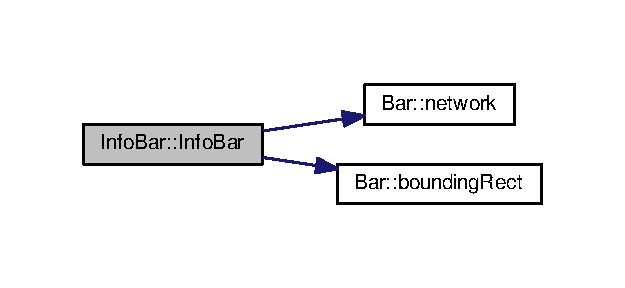
\includegraphics[width=300pt]{class_info_bar_aab5c08f226901c8827a97efbdfb5122a_cgraph}
\end{center}
\end{figure}


\hypertarget{class_info_bar_a954baa28d750739c80c029818d267d8e}{}\index{Info\+Bar@{Info\+Bar}!````~Info\+Bar@{$\sim$\+Info\+Bar}}
\index{````~Info\+Bar@{$\sim$\+Info\+Bar}!Info\+Bar@{Info\+Bar}}
\paragraph[{$\sim$\+Info\+Bar}]{\setlength{\rightskip}{0pt plus 5cm}Info\+Bar\+::$\sim$\+Info\+Bar (
\begin{DoxyParamCaption}
{}
\end{DoxyParamCaption}
)}\label{class_info_bar_a954baa28d750739c80c029818d267d8e}


Definition at line \hyperlink{infobar_8cpp_source_l00021}{21} of file \hyperlink{infobar_8cpp_source}{infobar.\+cpp}.



\subsubsection{Member Function Documentation}
\hypertarget{class_info_bar_a564aacb3b64bdb5fbcaef8a432a0b49e}{}\index{Info\+Bar@{Info\+Bar}!bounding\+Rect@{bounding\+Rect}}
\index{bounding\+Rect@{bounding\+Rect}!Info\+Bar@{Info\+Bar}}
\paragraph[{bounding\+Rect}]{\setlength{\rightskip}{0pt plus 5cm}Q\+Rect\+F Info\+Bar\+::bounding\+Rect (
\begin{DoxyParamCaption}
{}
\end{DoxyParamCaption}
) const}\label{class_info_bar_a564aacb3b64bdb5fbcaef8a432a0b49e}


Definition at line \hyperlink{infobar_8cpp_source_l00176}{176} of file \hyperlink{infobar_8cpp_source}{infobar.\+cpp}.

\hypertarget{class_info_bar_afa011ce96bb99021d2cbf5b24c7276bb}{}\index{Info\+Bar@{Info\+Bar}!paint@{paint}}
\index{paint@{paint}!Info\+Bar@{Info\+Bar}}
\paragraph[{paint}]{\setlength{\rightskip}{0pt plus 5cm}void Info\+Bar\+::paint (
\begin{DoxyParamCaption}
\item[{Q\+Painter $\ast$}]{painter, }
\item[{const Q\+Style\+Option\+Graphics\+Item $\ast$}]{option, }
\item[{Q\+Widget $\ast$}]{widget}
\end{DoxyParamCaption}
)\hspace{0.3cm}{\ttfamily [protected]}}\label{class_info_bar_afa011ce96bb99021d2cbf5b24c7276bb}


Definition at line \hyperlink{infobar_8cpp_source_l00023}{23} of file \hyperlink{infobar_8cpp_source}{infobar.\+cpp}.



\subsubsection{Member Data Documentation}
\hypertarget{class_info_bar_a28fb5e5d6d399d9327f67aa768d4a3d8}{}\index{Info\+Bar@{Info\+Bar}!k\+Box\+Base\+Height@{k\+Box\+Base\+Height}}
\index{k\+Box\+Base\+Height@{k\+Box\+Base\+Height}!Info\+Bar@{Info\+Bar}}
\paragraph[{k\+Box\+Base\+Height}]{\setlength{\rightskip}{0pt plus 5cm}const qreal Info\+Bar\+::k\+Box\+Base\+Height = 30.\+0\hspace{0.3cm}{\ttfamily [static]}}\label{class_info_bar_a28fb5e5d6d399d9327f67aa768d4a3d8}


Definition at line \hyperlink{infobar_8h_source_l00039}{39} of file \hyperlink{infobar_8h_source}{infobar.\+h}.

\hypertarget{class_info_bar_acb9c812df3577ae628cec2e149c9dd0a}{}\index{Info\+Bar@{Info\+Bar}!k\+Box\+Base\+Width@{k\+Box\+Base\+Width}}
\index{k\+Box\+Base\+Width@{k\+Box\+Base\+Width}!Info\+Bar@{Info\+Bar}}
\paragraph[{k\+Box\+Base\+Width}]{\setlength{\rightskip}{0pt plus 5cm}const qreal Info\+Bar\+::k\+Box\+Base\+Width = 60.\+0\hspace{0.3cm}{\ttfamily [static]}}\label{class_info_bar_acb9c812df3577ae628cec2e149c9dd0a}


Definition at line \hyperlink{infobar_8h_source_l00040}{40} of file \hyperlink{infobar_8h_source}{infobar.\+h}.

\hypertarget{class_info_bar_aba381a3838a5e064f1372f2f2b4d8e0d}{}\index{Info\+Bar@{Info\+Bar}!k\+Box\+Height@{k\+Box\+Height}}
\index{k\+Box\+Height@{k\+Box\+Height}!Info\+Bar@{Info\+Bar}}
\paragraph[{k\+Box\+Height}]{\setlength{\rightskip}{0pt plus 5cm}const qreal Info\+Bar\+::k\+Box\+Height = 37.\+5$\ast${\bf k\+Table\+Rows}\hspace{0.3cm}{\ttfamily [static]}}\label{class_info_bar_aba381a3838a5e064f1372f2f2b4d8e0d}


Definition at line \hyperlink{infobar_8h_source_l00020}{20} of file \hyperlink{infobar_8h_source}{infobar.\+h}.

\hypertarget{class_info_bar_aa1c35ddbae0324743d90721037447571}{}\index{Info\+Bar@{Info\+Bar}!k\+Box\+Width@{k\+Box\+Width}}
\index{k\+Box\+Width@{k\+Box\+Width}!Info\+Bar@{Info\+Bar}}
\paragraph[{k\+Box\+Width}]{\setlength{\rightskip}{0pt plus 5cm}const qreal Info\+Bar\+::k\+Box\+Width = 135.\+0$\ast${\bf k\+Table\+Colums}\hspace{0.3cm}{\ttfamily [static]}}\label{class_info_bar_aa1c35ddbae0324743d90721037447571}


Definition at line \hyperlink{infobar_8h_source_l00019}{19} of file \hyperlink{infobar_8h_source}{infobar.\+h}.

\hypertarget{class_info_bar_a46d929f42476a6ad37422adee1783712}{}\index{Info\+Bar@{Info\+Bar}!k\+Line\+Width@{k\+Line\+Width}}
\index{k\+Line\+Width@{k\+Line\+Width}!Info\+Bar@{Info\+Bar}}
\paragraph[{k\+Line\+Width}]{\setlength{\rightskip}{0pt plus 5cm}const qreal Info\+Bar\+::k\+Line\+Width = 2.\+0\hspace{0.3cm}{\ttfamily [static]}}\label{class_info_bar_a46d929f42476a6ad37422adee1783712}


Definition at line \hyperlink{infobar_8h_source_l00021}{21} of file \hyperlink{infobar_8h_source}{infobar.\+h}.

\hypertarget{class_info_bar_a67eb740893ed91c75f237cee756648cc}{}\index{Info\+Bar@{Info\+Bar}!k\+Margin\+Bot@{k\+Margin\+Bot}}
\index{k\+Margin\+Bot@{k\+Margin\+Bot}!Info\+Bar@{Info\+Bar}}
\paragraph[{k\+Margin\+Bot}]{\setlength{\rightskip}{0pt plus 5cm}const qreal Info\+Bar\+::k\+Margin\+Bot = 5.\+0\hspace{0.3cm}{\ttfamily [static]}}\label{class_info_bar_a67eb740893ed91c75f237cee756648cc}


Definition at line \hyperlink{infobar_8h_source_l00029}{29} of file \hyperlink{infobar_8h_source}{infobar.\+h}.

\hypertarget{class_info_bar_a0cfbafbc9f780fc1366157b9c8379463}{}\index{Info\+Bar@{Info\+Bar}!k\+Margin\+Head\+Bot@{k\+Margin\+Head\+Bot}}
\index{k\+Margin\+Head\+Bot@{k\+Margin\+Head\+Bot}!Info\+Bar@{Info\+Bar}}
\paragraph[{k\+Margin\+Head\+Bot}]{\setlength{\rightskip}{0pt plus 5cm}const qreal Info\+Bar\+::k\+Margin\+Head\+Bot = 5.\+0\hspace{0.3cm}{\ttfamily [static]}}\label{class_info_bar_a0cfbafbc9f780fc1366157b9c8379463}


Definition at line \hyperlink{infobar_8h_source_l00025}{25} of file \hyperlink{infobar_8h_source}{infobar.\+h}.

\hypertarget{class_info_bar_ae24b5cac460550a4c86203a3dbd96ba9}{}\index{Info\+Bar@{Info\+Bar}!k\+Margin\+Head\+Top@{k\+Margin\+Head\+Top}}
\index{k\+Margin\+Head\+Top@{k\+Margin\+Head\+Top}!Info\+Bar@{Info\+Bar}}
\paragraph[{k\+Margin\+Head\+Top}]{\setlength{\rightskip}{0pt plus 5cm}const qreal Info\+Bar\+::k\+Margin\+Head\+Top = 5.\+0\hspace{0.3cm}{\ttfamily [static]}}\label{class_info_bar_ae24b5cac460550a4c86203a3dbd96ba9}


Definition at line \hyperlink{infobar_8h_source_l00024}{24} of file \hyperlink{infobar_8h_source}{infobar.\+h}.

\hypertarget{class_info_bar_a3c7688259f189cb28c2682f50a59335a}{}\index{Info\+Bar@{Info\+Bar}!k\+Margin\+Left@{k\+Margin\+Left}}
\index{k\+Margin\+Left@{k\+Margin\+Left}!Info\+Bar@{Info\+Bar}}
\paragraph[{k\+Margin\+Left}]{\setlength{\rightskip}{0pt plus 5cm}const qreal Info\+Bar\+::k\+Margin\+Left = 5.\+0\hspace{0.3cm}{\ttfamily [static]}}\label{class_info_bar_a3c7688259f189cb28c2682f50a59335a}


Definition at line \hyperlink{infobar_8h_source_l00030}{30} of file \hyperlink{infobar_8h_source}{infobar.\+h}.

\hypertarget{class_info_bar_a2ce020e319adf3de887bf17e803887a3}{}\index{Info\+Bar@{Info\+Bar}!k\+Margin\+Right@{k\+Margin\+Right}}
\index{k\+Margin\+Right@{k\+Margin\+Right}!Info\+Bar@{Info\+Bar}}
\paragraph[{k\+Margin\+Right}]{\setlength{\rightskip}{0pt plus 5cm}const qreal Info\+Bar\+::k\+Margin\+Right = 5.\+0\hspace{0.3cm}{\ttfamily [static]}}\label{class_info_bar_a2ce020e319adf3de887bf17e803887a3}


Definition at line \hyperlink{infobar_8h_source_l00031}{31} of file \hyperlink{infobar_8h_source}{infobar.\+h}.

\hypertarget{class_info_bar_add145842c6a2331a7edf9e5be301e5b4}{}\index{Info\+Bar@{Info\+Bar}!k\+Margin\+Top@{k\+Margin\+Top}}
\index{k\+Margin\+Top@{k\+Margin\+Top}!Info\+Bar@{Info\+Bar}}
\paragraph[{k\+Margin\+Top}]{\setlength{\rightskip}{0pt plus 5cm}const qreal Info\+Bar\+::k\+Margin\+Top = 5.\+0\hspace{0.3cm}{\ttfamily [static]}}\label{class_info_bar_add145842c6a2331a7edf9e5be301e5b4}


Definition at line \hyperlink{infobar_8h_source_l00028}{28} of file \hyperlink{infobar_8h_source}{infobar.\+h}.

\hypertarget{class_info_bar_a57e9e7c40a6fd2a56dd47a4512d65489}{}\index{Info\+Bar@{Info\+Bar}!k\+Table\+Colums@{k\+Table\+Colums}}
\index{k\+Table\+Colums@{k\+Table\+Colums}!Info\+Bar@{Info\+Bar}}
\paragraph[{k\+Table\+Colums}]{\setlength{\rightskip}{0pt plus 5cm}const int Info\+Bar\+::k\+Table\+Colums = 3\hspace{0.3cm}{\ttfamily [static]}}\label{class_info_bar_a57e9e7c40a6fd2a56dd47a4512d65489}


Definition at line \hyperlink{infobar_8h_source_l00016}{16} of file \hyperlink{infobar_8h_source}{infobar.\+h}.

\hypertarget{class_info_bar_a8d9aadb8292b5884eb1c02e18d36d073}{}\index{Info\+Bar@{Info\+Bar}!k\+Table\+Line\+Width@{k\+Table\+Line\+Width}}
\index{k\+Table\+Line\+Width@{k\+Table\+Line\+Width}!Info\+Bar@{Info\+Bar}}
\paragraph[{k\+Table\+Line\+Width}]{\setlength{\rightskip}{0pt plus 5cm}const qreal Info\+Bar\+::k\+Table\+Line\+Width = 1.\+0\hspace{0.3cm}{\ttfamily [static]}}\label{class_info_bar_a8d9aadb8292b5884eb1c02e18d36d073}


Definition at line \hyperlink{infobar_8h_source_l00034}{34} of file \hyperlink{infobar_8h_source}{infobar.\+h}.

\hypertarget{class_info_bar_ad54d2dd19a63caf9d2476aace60ae3c5}{}\index{Info\+Bar@{Info\+Bar}!k\+Table\+Rows@{k\+Table\+Rows}}
\index{k\+Table\+Rows@{k\+Table\+Rows}!Info\+Bar@{Info\+Bar}}
\paragraph[{k\+Table\+Rows}]{\setlength{\rightskip}{0pt plus 5cm}const int Info\+Bar\+::k\+Table\+Rows = 4\hspace{0.3cm}{\ttfamily [static]}}\label{class_info_bar_ad54d2dd19a63caf9d2476aace60ae3c5}


Definition at line \hyperlink{infobar_8h_source_l00015}{15} of file \hyperlink{infobar_8h_source}{infobar.\+h}.

\hypertarget{class_info_bar_a8455611d11236c2d5cbd42414450e6e2}{}\index{Info\+Bar@{Info\+Bar}!k\+Text\+To\+Line\+Pad@{k\+Text\+To\+Line\+Pad}}
\index{k\+Text\+To\+Line\+Pad@{k\+Text\+To\+Line\+Pad}!Info\+Bar@{Info\+Bar}}
\paragraph[{k\+Text\+To\+Line\+Pad}]{\setlength{\rightskip}{0pt plus 5cm}const qreal Info\+Bar\+::k\+Text\+To\+Line\+Pad = 1.\+0\hspace{0.3cm}{\ttfamily [static]}}\label{class_info_bar_a8455611d11236c2d5cbd42414450e6e2}


Definition at line \hyperlink{infobar_8h_source_l00035}{35} of file \hyperlink{infobar_8h_source}{infobar.\+h}.



The documentation for this class was generated from the following files\+:\begin{DoxyCompactItemize}
\item 
\hyperlink{infobar_8h}{infobar.\+h}\item 
\hyperlink{infobar_8cpp}{infobar.\+cpp}\end{DoxyCompactItemize}

\hypertarget{class_info_line}{}\subsection{Info\+Line Class Reference}
\label{class_info_line}\index{Info\+Line@{Info\+Line}}


Inheritance diagram for Info\+Line\+:
\nopagebreak
\begin{figure}[H]
\begin{center}
\leavevmode
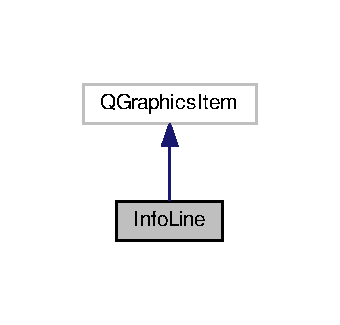
\includegraphics[width=163pt]{class_info_line__inherit__graph}
\end{center}
\end{figure}


Collaboration diagram for Info\+Line\+:
\nopagebreak
\begin{figure}[H]
\begin{center}
\leavevmode
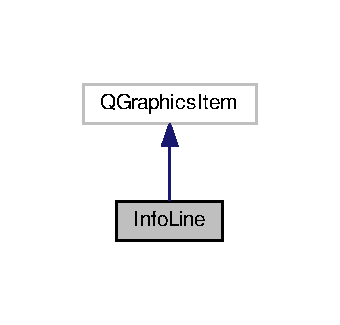
\includegraphics[width=163pt]{class_info_line__coll__graph}
\end{center}
\end{figure}
\subsubsection*{Public Member Functions}
\begin{DoxyCompactItemize}
\item 
\hyperlink{class_info_line_a63819dbfeb257cc86be86f0fac3aa02f}{Info\+Line} (\hyperlink{class_line}{Line} $\ast$line)
\item 
\hyperlink{class_info_line_ac3497eeb5f2719fb4fac42434955597d}{$\sim$\+Info\+Line} ()
\item 
Q\+Rect\+F \hyperlink{class_info_line_a3103eee5d5a8b4fd53d428f9aea01830}{bounding\+Rect} () const Q\+\_\+\+D\+E\+C\+L\+\_\+\+O\+V\+E\+R\+R\+I\+D\+E
\end{DoxyCompactItemize}
\subsubsection*{Static Public Attributes}
\begin{DoxyCompactItemize}
\item 
static const int \hyperlink{class_info_line_a95cdc7a95cde6db7c6faceda995d26b9}{k\+Table\+Rows} = 4
\item 
static const int \hyperlink{class_info_line_a9fc071b08eb913cf3afc623835ad2fd8}{k\+Table\+Colums} = 3
\item 
static const double \hyperlink{class_info_line_a33821aa140dc03829357d4006e9c153c}{k\+Box\+Width} = 135.\+0$\ast$\hyperlink{class_info_line_a9fc071b08eb913cf3afc623835ad2fd8}{k\+Table\+Colums}
\item 
static const double \hyperlink{class_info_line_a9e459549795bab79ae3b6c184dc78a00}{k\+Box\+Height} = 37.\+5$\ast$\hyperlink{class_info_line_a95cdc7a95cde6db7c6faceda995d26b9}{k\+Table\+Rows}
\item 
static const double \hyperlink{class_info_line_ad072bc8ef178113c36c3d480c7d637ac}{k\+Line\+Width} = 2.\+0
\item 
static const double \hyperlink{class_info_line_a73e02db68396f0c4b66d0cf80bd37c83}{k\+Margin\+Head\+Top} = 5.\+0
\item 
static const double \hyperlink{class_info_line_a82ed1944ec4a41af19e377a243c2332d}{k\+Margin\+Head\+Bot} = 5.\+0
\item 
static const double \hyperlink{class_info_line_a995100424420038664880195f5e51f50}{k\+Margin\+Top} = 5.\+0
\item 
static const double \hyperlink{class_info_line_ab4bd85105aabcb9d1230225c15873da2}{k\+Margin\+Bot} = 5.\+0
\item 
static const double \hyperlink{class_info_line_a68232e6e5e3b63a4b6aced3d99291ad7}{k\+Margin\+Left} = 5.\+0
\item 
static const double \hyperlink{class_info_line_a0f0bd713ed9c1c8012bbd29dbd1db75e}{k\+Margin\+Right} = 5.\+0
\item 
static const double \hyperlink{class_info_line_ab50f47aa54c45def219859e9da3755e6}{k\+Box\+Base\+Height} = 30.\+0
\item 
static const double \hyperlink{class_info_line_aad905589137b80ba75d9a1c49535eb1a}{k\+Box\+Base\+Width} = 60.\+0
\end{DoxyCompactItemize}
\subsubsection*{Protected Member Functions}
\begin{DoxyCompactItemize}
\item 
void \hyperlink{class_info_line_ac696c9944716774dfe85a40ac5a434e1}{paint} (Q\+Painter $\ast$painter, const Q\+Style\+Option\+Graphics\+Item $\ast$option, Q\+Widget $\ast$widget) Q\+\_\+\+D\+E\+C\+L\+\_\+\+O\+V\+E\+R\+R\+I\+D\+E
\item 
void \hyperlink{class_info_line_a389ea4f5085b60d03022b94e636f11d1}{set\+Head\+Font} (Q\+Painter $\ast$painter)
\item 
void \hyperlink{class_info_line_a4d5084d616c878cb717e8445db0023c1}{set\+Normal\+Font} (Q\+Painter $\ast$painter)
\item 
void \hyperlink{class_info_line_a3a0f83ad98fe674513dab679e22cba42}{draw\+Main\+Rectangle} (Q\+Rect\+F main\+Rect, double line\+Width, Q\+Painter $\ast$painter)
\item 
void \hyperlink{class_info_line_a53e9012a9cef4f07f1d4872c6d250c08}{draw\+Head\+Separator} (Q\+Rect\+F head\+Rect, Q\+Painter $\ast$painter)
\item 
void \hyperlink{class_info_line_a043932fa92604badc063e09691195609}{draw\+Head\+Text} (Q\+Rect\+F head\+Rect, double margin\+Top, Q\+String \&text, Q\+Painter $\ast$painter)
\end{DoxyCompactItemize}


\subsubsection{Detailed Description}


Definition at line \hyperlink{infoline_8h_source_l00012}{12} of file \hyperlink{infoline_8h_source}{infoline.\+h}.



\subsubsection{Constructor \& Destructor Documentation}
\hypertarget{class_info_line_a63819dbfeb257cc86be86f0fac3aa02f}{}\index{Info\+Line@{Info\+Line}!Info\+Line@{Info\+Line}}
\index{Info\+Line@{Info\+Line}!Info\+Line@{Info\+Line}}
\paragraph[{Info\+Line}]{\setlength{\rightskip}{0pt plus 5cm}Info\+Line\+::\+Info\+Line (
\begin{DoxyParamCaption}
\item[{{\bf Line} $\ast$}]{line}
\end{DoxyParamCaption}
)}\label{class_info_line_a63819dbfeb257cc86be86f0fac3aa02f}


Definition at line \hyperlink{infoline_8cpp_source_l00030}{30} of file \hyperlink{infoline_8cpp_source}{infoline.\+cpp}.



Here is the call graph for this function\+:
\nopagebreak
\begin{figure}[H]
\begin{center}
\leavevmode
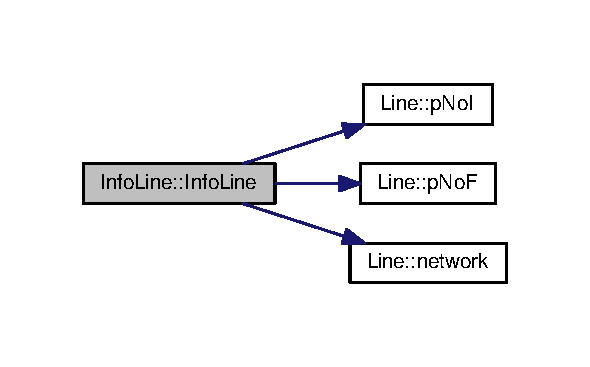
\includegraphics[width=283pt]{class_info_line_a63819dbfeb257cc86be86f0fac3aa02f_cgraph}
\end{center}
\end{figure}


\hypertarget{class_info_line_ac3497eeb5f2719fb4fac42434955597d}{}\index{Info\+Line@{Info\+Line}!````~Info\+Line@{$\sim$\+Info\+Line}}
\index{````~Info\+Line@{$\sim$\+Info\+Line}!Info\+Line@{Info\+Line}}
\paragraph[{$\sim$\+Info\+Line}]{\setlength{\rightskip}{0pt plus 5cm}Info\+Line\+::$\sim$\+Info\+Line (
\begin{DoxyParamCaption}
{}
\end{DoxyParamCaption}
)}\label{class_info_line_ac3497eeb5f2719fb4fac42434955597d}


Definition at line \hyperlink{infoline_8cpp_source_l00045}{45} of file \hyperlink{infoline_8cpp_source}{infoline.\+cpp}.



\subsubsection{Member Function Documentation}
\hypertarget{class_info_line_a3103eee5d5a8b4fd53d428f9aea01830}{}\index{Info\+Line@{Info\+Line}!bounding\+Rect@{bounding\+Rect}}
\index{bounding\+Rect@{bounding\+Rect}!Info\+Line@{Info\+Line}}
\paragraph[{bounding\+Rect}]{\setlength{\rightskip}{0pt plus 5cm}Q\+Rect\+F Info\+Line\+::bounding\+Rect (
\begin{DoxyParamCaption}
{}
\end{DoxyParamCaption}
) const}\label{class_info_line_a3103eee5d5a8b4fd53d428f9aea01830}


Definition at line \hyperlink{infoline_8cpp_source_l00241}{241} of file \hyperlink{infoline_8cpp_source}{infoline.\+cpp}.

\hypertarget{class_info_line_a53e9012a9cef4f07f1d4872c6d250c08}{}\index{Info\+Line@{Info\+Line}!draw\+Head\+Separator@{draw\+Head\+Separator}}
\index{draw\+Head\+Separator@{draw\+Head\+Separator}!Info\+Line@{Info\+Line}}
\paragraph[{draw\+Head\+Separator}]{\setlength{\rightskip}{0pt plus 5cm}void Info\+Line\+::draw\+Head\+Separator (
\begin{DoxyParamCaption}
\item[{Q\+Rect\+F}]{head\+Rect, }
\item[{Q\+Painter $\ast$}]{painter}
\end{DoxyParamCaption}
)\hspace{0.3cm}{\ttfamily [protected]}}\label{class_info_line_a53e9012a9cef4f07f1d4872c6d250c08}


Definition at line \hyperlink{infoline_8cpp_source_l00217}{217} of file \hyperlink{infoline_8cpp_source}{infoline.\+cpp}.



Here is the caller graph for this function\+:
\nopagebreak
\begin{figure}[H]
\begin{center}
\leavevmode
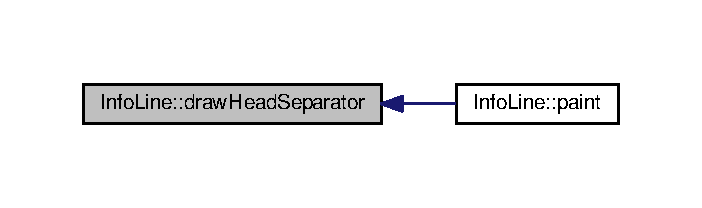
\includegraphics[width=337pt]{class_info_line_a53e9012a9cef4f07f1d4872c6d250c08_icgraph}
\end{center}
\end{figure}


\hypertarget{class_info_line_a043932fa92604badc063e09691195609}{}\index{Info\+Line@{Info\+Line}!draw\+Head\+Text@{draw\+Head\+Text}}
\index{draw\+Head\+Text@{draw\+Head\+Text}!Info\+Line@{Info\+Line}}
\paragraph[{draw\+Head\+Text}]{\setlength{\rightskip}{0pt plus 5cm}void Info\+Line\+::draw\+Head\+Text (
\begin{DoxyParamCaption}
\item[{Q\+Rect\+F}]{head\+Rect, }
\item[{double}]{margin\+Top, }
\item[{Q\+String \&}]{text, }
\item[{Q\+Painter $\ast$}]{painter}
\end{DoxyParamCaption}
)\hspace{0.3cm}{\ttfamily [protected]}}\label{class_info_line_a043932fa92604badc063e09691195609}


Definition at line \hyperlink{infoline_8cpp_source_l00229}{229} of file \hyperlink{infoline_8cpp_source}{infoline.\+cpp}.



Here is the caller graph for this function\+:
\nopagebreak
\begin{figure}[H]
\begin{center}
\leavevmode
\includegraphics[width=315pt]{class_info_line_a043932fa92604badc063e09691195609_icgraph}
\end{center}
\end{figure}


\hypertarget{class_info_line_a3a0f83ad98fe674513dab679e22cba42}{}\index{Info\+Line@{Info\+Line}!draw\+Main\+Rectangle@{draw\+Main\+Rectangle}}
\index{draw\+Main\+Rectangle@{draw\+Main\+Rectangle}!Info\+Line@{Info\+Line}}
\paragraph[{draw\+Main\+Rectangle}]{\setlength{\rightskip}{0pt plus 5cm}void Info\+Line\+::draw\+Main\+Rectangle (
\begin{DoxyParamCaption}
\item[{Q\+Rect\+F}]{main\+Rect, }
\item[{double}]{line\+Width, }
\item[{Q\+Painter $\ast$}]{painter}
\end{DoxyParamCaption}
)\hspace{0.3cm}{\ttfamily [protected]}}\label{class_info_line_a3a0f83ad98fe674513dab679e22cba42}


Definition at line \hyperlink{infoline_8cpp_source_l00204}{204} of file \hyperlink{infoline_8cpp_source}{infoline.\+cpp}.



Here is the caller graph for this function\+:
\nopagebreak
\begin{figure}[H]
\begin{center}
\leavevmode
\includegraphics[width=337pt]{class_info_line_a3a0f83ad98fe674513dab679e22cba42_icgraph}
\end{center}
\end{figure}


\hypertarget{class_info_line_ac696c9944716774dfe85a40ac5a434e1}{}\index{Info\+Line@{Info\+Line}!paint@{paint}}
\index{paint@{paint}!Info\+Line@{Info\+Line}}
\paragraph[{paint}]{\setlength{\rightskip}{0pt plus 5cm}void Info\+Line\+::paint (
\begin{DoxyParamCaption}
\item[{Q\+Painter $\ast$}]{painter, }
\item[{const Q\+Style\+Option\+Graphics\+Item $\ast$}]{option, }
\item[{Q\+Widget $\ast$}]{widget}
\end{DoxyParamCaption}
)\hspace{0.3cm}{\ttfamily [protected]}}\label{class_info_line_ac696c9944716774dfe85a40ac5a434e1}


Definition at line \hyperlink{infoline_8cpp_source_l00053}{53} of file \hyperlink{infoline_8cpp_source}{infoline.\+cpp}.



Here is the call graph for this function\+:
\nopagebreak
\begin{figure}[H]
\begin{center}
\leavevmode
\includegraphics[width=337pt]{class_info_line_ac696c9944716774dfe85a40ac5a434e1_cgraph}
\end{center}
\end{figure}


\hypertarget{class_info_line_a389ea4f5085b60d03022b94e636f11d1}{}\index{Info\+Line@{Info\+Line}!set\+Head\+Font@{set\+Head\+Font}}
\index{set\+Head\+Font@{set\+Head\+Font}!Info\+Line@{Info\+Line}}
\paragraph[{set\+Head\+Font}]{\setlength{\rightskip}{0pt plus 5cm}void Info\+Line\+::set\+Head\+Font (
\begin{DoxyParamCaption}
\item[{Q\+Painter $\ast$}]{painter}
\end{DoxyParamCaption}
)\hspace{0.3cm}{\ttfamily [protected]}}\label{class_info_line_a389ea4f5085b60d03022b94e636f11d1}


Definition at line \hyperlink{infoline_8cpp_source_l00182}{182} of file \hyperlink{infoline_8cpp_source}{infoline.\+cpp}.



Here is the caller graph for this function\+:
\nopagebreak
\begin{figure}[H]
\begin{center}
\leavevmode
\includegraphics[width=307pt]{class_info_line_a389ea4f5085b60d03022b94e636f11d1_icgraph}
\end{center}
\end{figure}


\hypertarget{class_info_line_a4d5084d616c878cb717e8445db0023c1}{}\index{Info\+Line@{Info\+Line}!set\+Normal\+Font@{set\+Normal\+Font}}
\index{set\+Normal\+Font@{set\+Normal\+Font}!Info\+Line@{Info\+Line}}
\paragraph[{set\+Normal\+Font}]{\setlength{\rightskip}{0pt plus 5cm}void Info\+Line\+::set\+Normal\+Font (
\begin{DoxyParamCaption}
\item[{Q\+Painter $\ast$}]{painter}
\end{DoxyParamCaption}
)\hspace{0.3cm}{\ttfamily [protected]}}\label{class_info_line_a4d5084d616c878cb717e8445db0023c1}


Definition at line \hyperlink{infoline_8cpp_source_l00193}{193} of file \hyperlink{infoline_8cpp_source}{infoline.\+cpp}.



Here is the caller graph for this function\+:
\nopagebreak
\begin{figure}[H]
\begin{center}
\leavevmode
\includegraphics[width=316pt]{class_info_line_a4d5084d616c878cb717e8445db0023c1_icgraph}
\end{center}
\end{figure}




\subsubsection{Member Data Documentation}
\hypertarget{class_info_line_ab50f47aa54c45def219859e9da3755e6}{}\index{Info\+Line@{Info\+Line}!k\+Box\+Base\+Height@{k\+Box\+Base\+Height}}
\index{k\+Box\+Base\+Height@{k\+Box\+Base\+Height}!Info\+Line@{Info\+Line}}
\paragraph[{k\+Box\+Base\+Height}]{\setlength{\rightskip}{0pt plus 5cm}const double Info\+Line\+::k\+Box\+Base\+Height = 30.\+0\hspace{0.3cm}{\ttfamily [static]}}\label{class_info_line_ab50f47aa54c45def219859e9da3755e6}


Definition at line \hyperlink{infoline_8h_source_l00034}{34} of file \hyperlink{infoline_8h_source}{infoline.\+h}.

\hypertarget{class_info_line_aad905589137b80ba75d9a1c49535eb1a}{}\index{Info\+Line@{Info\+Line}!k\+Box\+Base\+Width@{k\+Box\+Base\+Width}}
\index{k\+Box\+Base\+Width@{k\+Box\+Base\+Width}!Info\+Line@{Info\+Line}}
\paragraph[{k\+Box\+Base\+Width}]{\setlength{\rightskip}{0pt plus 5cm}const double Info\+Line\+::k\+Box\+Base\+Width = 60.\+0\hspace{0.3cm}{\ttfamily [static]}}\label{class_info_line_aad905589137b80ba75d9a1c49535eb1a}


Definition at line \hyperlink{infoline_8h_source_l00035}{35} of file \hyperlink{infoline_8h_source}{infoline.\+h}.

\hypertarget{class_info_line_a9e459549795bab79ae3b6c184dc78a00}{}\index{Info\+Line@{Info\+Line}!k\+Box\+Height@{k\+Box\+Height}}
\index{k\+Box\+Height@{k\+Box\+Height}!Info\+Line@{Info\+Line}}
\paragraph[{k\+Box\+Height}]{\setlength{\rightskip}{0pt plus 5cm}const double Info\+Line\+::k\+Box\+Height = 37.\+5$\ast${\bf k\+Table\+Rows}\hspace{0.3cm}{\ttfamily [static]}}\label{class_info_line_a9e459549795bab79ae3b6c184dc78a00}


Definition at line \hyperlink{infoline_8h_source_l00020}{20} of file \hyperlink{infoline_8h_source}{infoline.\+h}.

\hypertarget{class_info_line_a33821aa140dc03829357d4006e9c153c}{}\index{Info\+Line@{Info\+Line}!k\+Box\+Width@{k\+Box\+Width}}
\index{k\+Box\+Width@{k\+Box\+Width}!Info\+Line@{Info\+Line}}
\paragraph[{k\+Box\+Width}]{\setlength{\rightskip}{0pt plus 5cm}const double Info\+Line\+::k\+Box\+Width = 135.\+0$\ast${\bf k\+Table\+Colums}\hspace{0.3cm}{\ttfamily [static]}}\label{class_info_line_a33821aa140dc03829357d4006e9c153c}


Definition at line \hyperlink{infoline_8h_source_l00019}{19} of file \hyperlink{infoline_8h_source}{infoline.\+h}.

\hypertarget{class_info_line_ad072bc8ef178113c36c3d480c7d637ac}{}\index{Info\+Line@{Info\+Line}!k\+Line\+Width@{k\+Line\+Width}}
\index{k\+Line\+Width@{k\+Line\+Width}!Info\+Line@{Info\+Line}}
\paragraph[{k\+Line\+Width}]{\setlength{\rightskip}{0pt plus 5cm}const double Info\+Line\+::k\+Line\+Width = 2.\+0\hspace{0.3cm}{\ttfamily [static]}}\label{class_info_line_ad072bc8ef178113c36c3d480c7d637ac}


Definition at line \hyperlink{infoline_8h_source_l00021}{21} of file \hyperlink{infoline_8h_source}{infoline.\+h}.

\hypertarget{class_info_line_ab4bd85105aabcb9d1230225c15873da2}{}\index{Info\+Line@{Info\+Line}!k\+Margin\+Bot@{k\+Margin\+Bot}}
\index{k\+Margin\+Bot@{k\+Margin\+Bot}!Info\+Line@{Info\+Line}}
\paragraph[{k\+Margin\+Bot}]{\setlength{\rightskip}{0pt plus 5cm}const double Info\+Line\+::k\+Margin\+Bot = 5.\+0\hspace{0.3cm}{\ttfamily [static]}}\label{class_info_line_ab4bd85105aabcb9d1230225c15873da2}


Definition at line \hyperlink{infoline_8h_source_l00029}{29} of file \hyperlink{infoline_8h_source}{infoline.\+h}.

\hypertarget{class_info_line_a82ed1944ec4a41af19e377a243c2332d}{}\index{Info\+Line@{Info\+Line}!k\+Margin\+Head\+Bot@{k\+Margin\+Head\+Bot}}
\index{k\+Margin\+Head\+Bot@{k\+Margin\+Head\+Bot}!Info\+Line@{Info\+Line}}
\paragraph[{k\+Margin\+Head\+Bot}]{\setlength{\rightskip}{0pt plus 5cm}const double Info\+Line\+::k\+Margin\+Head\+Bot = 5.\+0\hspace{0.3cm}{\ttfamily [static]}}\label{class_info_line_a82ed1944ec4a41af19e377a243c2332d}


Definition at line \hyperlink{infoline_8h_source_l00025}{25} of file \hyperlink{infoline_8h_source}{infoline.\+h}.

\hypertarget{class_info_line_a73e02db68396f0c4b66d0cf80bd37c83}{}\index{Info\+Line@{Info\+Line}!k\+Margin\+Head\+Top@{k\+Margin\+Head\+Top}}
\index{k\+Margin\+Head\+Top@{k\+Margin\+Head\+Top}!Info\+Line@{Info\+Line}}
\paragraph[{k\+Margin\+Head\+Top}]{\setlength{\rightskip}{0pt plus 5cm}const double Info\+Line\+::k\+Margin\+Head\+Top = 5.\+0\hspace{0.3cm}{\ttfamily [static]}}\label{class_info_line_a73e02db68396f0c4b66d0cf80bd37c83}


Definition at line \hyperlink{infoline_8h_source_l00024}{24} of file \hyperlink{infoline_8h_source}{infoline.\+h}.

\hypertarget{class_info_line_a68232e6e5e3b63a4b6aced3d99291ad7}{}\index{Info\+Line@{Info\+Line}!k\+Margin\+Left@{k\+Margin\+Left}}
\index{k\+Margin\+Left@{k\+Margin\+Left}!Info\+Line@{Info\+Line}}
\paragraph[{k\+Margin\+Left}]{\setlength{\rightskip}{0pt plus 5cm}const double Info\+Line\+::k\+Margin\+Left = 5.\+0\hspace{0.3cm}{\ttfamily [static]}}\label{class_info_line_a68232e6e5e3b63a4b6aced3d99291ad7}


Definition at line \hyperlink{infoline_8h_source_l00030}{30} of file \hyperlink{infoline_8h_source}{infoline.\+h}.

\hypertarget{class_info_line_a0f0bd713ed9c1c8012bbd29dbd1db75e}{}\index{Info\+Line@{Info\+Line}!k\+Margin\+Right@{k\+Margin\+Right}}
\index{k\+Margin\+Right@{k\+Margin\+Right}!Info\+Line@{Info\+Line}}
\paragraph[{k\+Margin\+Right}]{\setlength{\rightskip}{0pt plus 5cm}const double Info\+Line\+::k\+Margin\+Right = 5.\+0\hspace{0.3cm}{\ttfamily [static]}}\label{class_info_line_a0f0bd713ed9c1c8012bbd29dbd1db75e}


Definition at line \hyperlink{infoline_8h_source_l00031}{31} of file \hyperlink{infoline_8h_source}{infoline.\+h}.

\hypertarget{class_info_line_a995100424420038664880195f5e51f50}{}\index{Info\+Line@{Info\+Line}!k\+Margin\+Top@{k\+Margin\+Top}}
\index{k\+Margin\+Top@{k\+Margin\+Top}!Info\+Line@{Info\+Line}}
\paragraph[{k\+Margin\+Top}]{\setlength{\rightskip}{0pt plus 5cm}const double Info\+Line\+::k\+Margin\+Top = 5.\+0\hspace{0.3cm}{\ttfamily [static]}}\label{class_info_line_a995100424420038664880195f5e51f50}


Definition at line \hyperlink{infoline_8h_source_l00028}{28} of file \hyperlink{infoline_8h_source}{infoline.\+h}.

\hypertarget{class_info_line_a9fc071b08eb913cf3afc623835ad2fd8}{}\index{Info\+Line@{Info\+Line}!k\+Table\+Colums@{k\+Table\+Colums}}
\index{k\+Table\+Colums@{k\+Table\+Colums}!Info\+Line@{Info\+Line}}
\paragraph[{k\+Table\+Colums}]{\setlength{\rightskip}{0pt plus 5cm}const int Info\+Line\+::k\+Table\+Colums = 3\hspace{0.3cm}{\ttfamily [static]}}\label{class_info_line_a9fc071b08eb913cf3afc623835ad2fd8}


Definition at line \hyperlink{infoline_8h_source_l00016}{16} of file \hyperlink{infoline_8h_source}{infoline.\+h}.

\hypertarget{class_info_line_a95cdc7a95cde6db7c6faceda995d26b9}{}\index{Info\+Line@{Info\+Line}!k\+Table\+Rows@{k\+Table\+Rows}}
\index{k\+Table\+Rows@{k\+Table\+Rows}!Info\+Line@{Info\+Line}}
\paragraph[{k\+Table\+Rows}]{\setlength{\rightskip}{0pt plus 5cm}const int Info\+Line\+::k\+Table\+Rows = 4\hspace{0.3cm}{\ttfamily [static]}}\label{class_info_line_a95cdc7a95cde6db7c6faceda995d26b9}


Definition at line \hyperlink{infoline_8h_source_l00015}{15} of file \hyperlink{infoline_8h_source}{infoline.\+h}.



The documentation for this class was generated from the following files\+:\begin{DoxyCompactItemize}
\item 
\hyperlink{infoline_8h}{infoline.\+h}\item 
\hyperlink{infoline_8cpp}{infoline.\+cpp}\end{DoxyCompactItemize}

\hypertarget{class_line}{}\subsection{Line Class Reference}
\label{class_line}\index{Line@{Line}}


Represents a cable in power distribution systems.  




Inheritance diagram for Line\+:\nopagebreak
\begin{figure}[H]
\begin{center}
\leavevmode
\includegraphics[width=172pt]{class_line__inherit__graph}
\end{center}
\end{figure}


Collaboration diagram for Line\+:\nopagebreak
\begin{figure}[H]
\begin{center}
\leavevmode
\includegraphics[width=244pt]{class_line__coll__graph}
\end{center}
\end{figure}
\subsubsection*{Signals}
\begin{DoxyCompactItemize}
\item 
void \hyperlink{class_line_a2444b577ea2254994599c6f829c629a5}{event\+Double\+Click} ()
\begin{DoxyCompactList}\small\item\em event\+Double\+Click \end{DoxyCompactList}\end{DoxyCompactItemize}
\subsubsection*{Public Member Functions}
\begin{DoxyCompactItemize}
\item 
\hyperlink{group___models_gacc11b8a429d8cdd63ba6803dff5602b3}{Line} ()
\item 
\hyperlink{group___models_gaabe85f48d22d92b62257091f48174fac}{$\sim$\+Line} ()
\item 
complex$<$ double $>$ \hyperlink{group___models_gab5370574fd93e13eb11742f7753fe1f1}{z} (int32\+\_\+t index, \hyperlink{class_unit_a3747e779c805df24a71961290be3fbdf}{Unit\+::\+Impedance\+Unit} unit=\hyperlink{class_unit_a3747e779c805df24a71961290be3fbdfa6b9c74d1763eefbaf751eeecff0bd9da}{Unit\+::k\+Ohm})
\item 
void \hyperlink{group___models_ga409df7d11f5c5d594a13fb2f74b3b9e0}{set\+Z} (int32\+\_\+t index, complex$<$ double $>$ new\+Impedance, \hyperlink{class_unit_a3747e779c805df24a71961290be3fbdf}{Unit\+::\+Impedance\+Unit} unit=\hyperlink{class_unit_a3747e779c805df24a71961290be3fbdfa6b9c74d1763eefbaf751eeecff0bd9da}{Unit\+::k\+Ohm})
\item 
complex$<$ double $>$ \hyperlink{group___models_gaf81e7055102816465bdf7e19afc2d547}{i} (int32\+\_\+t phase, \hyperlink{class_unit_a0794cf6c9682f48296dd4a5315389787}{Unit\+::\+Current\+Unit} unit=\hyperlink{class_unit_a0794cf6c9682f48296dd4a5315389787a368a3c470f0b590a6100dda717a7dd4f}{Unit\+::k\+Ampere})
\item 
void \hyperlink{group___models_ga9e55b06dc3e385838fdd13d5580438ef}{set\+I} (int32\+\_\+t phase, complex$<$ double $>$ new\+Current, \hyperlink{class_unit_a0794cf6c9682f48296dd4a5315389787}{Unit\+::\+Current\+Unit} unit=\hyperlink{class_unit_a0794cf6c9682f48296dd4a5315389787a368a3c470f0b590a6100dda717a7dd4f}{Unit\+::k\+Ampere})
\item 
complex$<$ double $>$ \hyperlink{group___models_ga7909d69e419de3f460ca7abab3d91e53}{loss} (int32\+\_\+t phase, \hyperlink{class_unit_ace265ae255370ccacfd5370337572c3b}{Unit\+::\+Power\+Unit})
\item 
double \hyperlink{group___models_gae2e4500d0fa60dcc2ecb08b2c96954f9}{length} (\hyperlink{class_unit_a8c8921f7b225ad6063b1cb573425b9a0}{Unit\+::\+Length\+Unit} unit=\hyperlink{class_unit_a8c8921f7b225ad6063b1cb573425b9a0abfa41ebe7ee649a1f02c9b8ae570434b}{Unit\+::k\+Meter})
\item 
void \hyperlink{group___models_ga950d0b8f5d167eda430c65ca7adadbb0}{set\+Length} (double new\+Length, \hyperlink{class_unit_a8c8921f7b225ad6063b1cb573425b9a0}{Unit\+::\+Length\+Unit} unit=\hyperlink{class_unit_a8c8921f7b225ad6063b1cb573425b9a0abfa41ebe7ee649a1f02c9b8ae570434b}{Unit\+::k\+Meter})
\item 
\hyperlink{class_bar}{Bar} $\ast$ \hyperlink{group___models_gaeafd90e84ac2f8de2a879abe9e53eef3}{p\+No\+I} ()
\item 
\hyperlink{class_bar}{Bar} $\ast$ \hyperlink{group___models_gabbc73ddedd3075c33ae5331bd7c9829f}{p\+No\+F} ()
\item 
void \hyperlink{group___models_gaeeab146e6c1d7d1a688a2764a9c9a170}{set\+Nodes} (\hyperlink{class_bar}{Bar} $\ast$\hyperlink{group___models_gaeafd90e84ac2f8de2a879abe9e53eef3}{p\+No\+I}, \hyperlink{class_bar}{Bar} $\ast$\hyperlink{group___models_gabbc73ddedd3075c33ae5331bd7c9829f}{p\+No\+F})
\item 
Q\+Json\+Object \hyperlink{group___models_ga4effa7a96db465ea6e01135d5a010739}{to\+Json} ()
\item 
void \hyperlink{group___models_ga62623ad71df5279377cc69da90decc75}{from\+Json} (Q\+Json\+Object \&line\+Json)
\item 
void \hyperlink{group___models_ga8fdb12651d4bc592616d241386b066b3}{update\+Position} ()
\item 
Q\+Rect\+F \hyperlink{group___models_gad15c3af158d3b966c04be7e18cee5aea}{bounding\+Rect} () const Q\+\_\+\+D\+E\+C\+L\+\_\+\+O\+V\+E\+R\+R\+I\+D\+E
\item 
Q\+Painter\+Path \hyperlink{group___models_gaf1736b829a643d99052ef6428ddd5b16}{shape} () const Q\+\_\+\+D\+E\+C\+L\+\_\+\+O\+V\+E\+R\+R\+I\+D\+E
\item 
Q\+Variant \hyperlink{group___models_ga5fcee3f23eb50e34f730d602a3802b93}{item\+Change} (Graphics\+Item\+Change change, const Q\+Variant \&value) Q\+\_\+\+D\+E\+C\+L\+\_\+\+O\+V\+E\+R\+R\+I\+D\+E
\end{DoxyCompactItemize}
\subsubsection*{Public Attributes}
\begin{DoxyCompactItemize}
\item 
Q\+Pair$<$ int32\+\_\+t, int32\+\_\+t $>$ \hyperlink{class_line_afd17c40d656e6a8d677cb22df5f0c70b}{nodes}
\item 
\hyperlink{class_network}{Network} $\ast$ \hyperlink{class_line_aefdf6a6c3e3775b5a16b344c1d33964e}{network}
\end{DoxyCompactItemize}
\subsubsection*{Static Public Attributes}
\begin{DoxyCompactItemize}
\item 
static const int32\+\_\+t \hyperlink{group___models_gadc334bd07c6126abc56e531d7e3e72b4}{k\+Invalid\+Node} = -\/1
\end{DoxyCompactItemize}
\subsubsection*{Protected Member Functions}
\begin{DoxyCompactItemize}
\item 
void \hyperlink{group___models_ga9a1fee5b1606ab0deedd04bdab99be70}{mouse\+Double\+Click\+Event} (Q\+Graphics\+Scene\+Mouse\+Event $\ast$event) Q\+\_\+\+D\+E\+C\+L\+\_\+\+O\+V\+E\+R\+R\+I\+D\+E
\begin{DoxyCompactList}\small\item\em mouse\+Double\+Click\+Event \end{DoxyCompactList}\item 
void \hyperlink{group___models_ga0aa64aed379d434be5942edf572b444b}{paint} (Q\+Painter $\ast$painter, const Q\+Style\+Option\+Graphics\+Item $\ast$option, Q\+Widget $\ast$widget) Q\+\_\+\+D\+E\+C\+L\+\_\+\+O\+V\+E\+R\+R\+I\+D\+E
\end{DoxyCompactItemize}


\subsubsection{Detailed Description}
\subparagraph*{Overview}

\hyperlink{class_line}{Line} class represents a line in a power system, providing the data structure and methods that model a real line.

\subparagraph*{Example}


\begin{DoxyCode}
\end{DoxyCode}
 

Definition at line \hyperlink{line_8h_source_l00074}{74} of file \hyperlink{line_8h_source}{line.\+h}.



\subsubsection{Member Function Documentation}
\hypertarget{class_line_a2444b577ea2254994599c6f829c629a5}{}\index{Line@{Line}!event\+Double\+Click@{event\+Double\+Click}}
\index{event\+Double\+Click@{event\+Double\+Click}!Line@{Line}}
\paragraph[{event\+Double\+Click}]{\setlength{\rightskip}{0pt plus 5cm}void Line\+::event\+Double\+Click (
\begin{DoxyParamCaption}
{}
\end{DoxyParamCaption}
)\hspace{0.3cm}{\ttfamily [signal]}}\label{class_line_a2444b577ea2254994599c6f829c629a5}


Here is the caller graph for this function\+:\nopagebreak
\begin{figure}[H]
\begin{center}
\leavevmode
\includegraphics[width=350pt]{class_line_a2444b577ea2254994599c6f829c629a5_icgraph}
\end{center}
\end{figure}




\subsubsection{Member Data Documentation}
\hypertarget{class_line_aefdf6a6c3e3775b5a16b344c1d33964e}{}\index{Line@{Line}!network@{network}}
\index{network@{network}!Line@{Line}}
\paragraph[{network}]{\setlength{\rightskip}{0pt plus 5cm}{\bf Network}$\ast$ Line\+::network}\label{class_line_aefdf6a6c3e3775b5a16b344c1d33964e}


Definition at line \hyperlink{line_8h_source_l00089}{89} of file \hyperlink{line_8h_source}{line.\+h}.

\hypertarget{class_line_afd17c40d656e6a8d677cb22df5f0c70b}{}\index{Line@{Line}!nodes@{nodes}}
\index{nodes@{nodes}!Line@{Line}}
\paragraph[{nodes}]{\setlength{\rightskip}{0pt plus 5cm}Q\+Pair$<$int32\+\_\+t, int32\+\_\+t$>$ Line\+::nodes}\label{class_line_afd17c40d656e6a8d677cb22df5f0c70b}


Definition at line \hyperlink{line_8h_source_l00087}{87} of file \hyperlink{line_8h_source}{line.\+h}.



The documentation for this class was generated from the following files\+:\begin{DoxyCompactItemize}
\item 
\hyperlink{line_8h}{line.\+h}\item 
\hyperlink{line_8cpp}{line.\+cpp}\end{DoxyCompactItemize}

\hypertarget{class_line_properties}{}\subsection{Line\+Properties Class Reference}
\label{class_line_properties}\index{Line\+Properties@{Line\+Properties}}


Inheritance diagram for Line\+Properties\+:
\nopagebreak
\begin{figure}[H]
\begin{center}
\leavevmode
\includegraphics[width=159pt]{class_line_properties__inherit__graph}
\end{center}
\end{figure}


Collaboration diagram for Line\+Properties\+:
\nopagebreak
\begin{figure}[H]
\begin{center}
\leavevmode
\includegraphics[width=159pt]{class_line_properties__coll__graph}
\end{center}
\end{figure}
\subsubsection*{Public Member Functions}
\begin{DoxyCompactItemize}
\item 
\hyperlink{class_line_properties_a0bc0d7c02db0a4ea920d040f76679fec}{Line\+Properties} (Q\+Widget $\ast$parent=0)
\item 
\hyperlink{class_line_properties_a59017a6580f2e02dc492522d9267de29}{$\sim$\+Line\+Properties} ()
\item 
void \hyperlink{class_line_properties_ad434fc8e65787648a44737fb9f46b475}{set\+Options} (\hyperlink{class_project}{Project} $\ast$project, \hyperlink{class_line}{Line} $\ast$line)
\end{DoxyCompactItemize}


\subsubsection{Detailed Description}


Definition at line \hyperlink{lineproperties_8h_source_l00017}{17} of file \hyperlink{lineproperties_8h_source}{lineproperties.\+h}.



\subsubsection{Constructor \& Destructor Documentation}
\hypertarget{class_line_properties_a0bc0d7c02db0a4ea920d040f76679fec}{}\index{Line\+Properties@{Line\+Properties}!Line\+Properties@{Line\+Properties}}
\index{Line\+Properties@{Line\+Properties}!Line\+Properties@{Line\+Properties}}
\paragraph[{Line\+Properties}]{\setlength{\rightskip}{0pt plus 5cm}Line\+Properties\+::\+Line\+Properties (
\begin{DoxyParamCaption}
\item[{Q\+Widget $\ast$}]{parent = {\ttfamily 0}}
\end{DoxyParamCaption}
)\hspace{0.3cm}{\ttfamily [explicit]}}\label{class_line_properties_a0bc0d7c02db0a4ea920d040f76679fec}


Definition at line \hyperlink{lineproperties_8cpp_source_l00008}{8} of file \hyperlink{lineproperties_8cpp_source}{lineproperties.\+cpp}.

\hypertarget{class_line_properties_a59017a6580f2e02dc492522d9267de29}{}\index{Line\+Properties@{Line\+Properties}!````~Line\+Properties@{$\sim$\+Line\+Properties}}
\index{````~Line\+Properties@{$\sim$\+Line\+Properties}!Line\+Properties@{Line\+Properties}}
\paragraph[{$\sim$\+Line\+Properties}]{\setlength{\rightskip}{0pt plus 5cm}Line\+Properties\+::$\sim$\+Line\+Properties (
\begin{DoxyParamCaption}
{}
\end{DoxyParamCaption}
)}\label{class_line_properties_a59017a6580f2e02dc492522d9267de29}


Definition at line \hyperlink{lineproperties_8cpp_source_l00021}{21} of file \hyperlink{lineproperties_8cpp_source}{lineproperties.\+cpp}.



\subsubsection{Member Function Documentation}
\hypertarget{class_line_properties_ad434fc8e65787648a44737fb9f46b475}{}\index{Line\+Properties@{Line\+Properties}!set\+Options@{set\+Options}}
\index{set\+Options@{set\+Options}!Line\+Properties@{Line\+Properties}}
\paragraph[{set\+Options}]{\setlength{\rightskip}{0pt plus 5cm}void Line\+Properties\+::set\+Options (
\begin{DoxyParamCaption}
\item[{{\bf Project} $\ast$}]{project, }
\item[{{\bf Line} $\ast$}]{line}
\end{DoxyParamCaption}
)}\label{class_line_properties_ad434fc8e65787648a44737fb9f46b475}


Definition at line \hyperlink{lineproperties_8cpp_source_l00029}{29} of file \hyperlink{lineproperties_8cpp_source}{lineproperties.\+cpp}.



The documentation for this class was generated from the following files\+:\begin{DoxyCompactItemize}
\item 
\hyperlink{lineproperties_8h}{lineproperties.\+h}\item 
\hyperlink{lineproperties_8cpp}{lineproperties.\+cpp}\end{DoxyCompactItemize}

\hypertarget{class_network}{}\subsection{Network Class Reference}
\label{class_network}\index{Network@{Network}}


Represents a power distribution systems.  




Inheritance diagram for Network\+:\nopagebreak
\begin{figure}[H]
\begin{center}
\leavevmode
\includegraphics[width=133pt]{class_network__inherit__graph}
\end{center}
\end{figure}


Collaboration diagram for Network\+:\nopagebreak
\begin{figure}[H]
\begin{center}
\leavevmode
\includegraphics[width=133pt]{class_network__coll__graph}
\end{center}
\end{figure}
\subsubsection*{Public Member Functions}
\begin{DoxyCompactItemize}
\item 
\hyperlink{group___graphics_ga3cc2fb4f8fa4d507077e8da85ce5a1c8}{Network} ()
\item 
\hyperlink{group___graphics_ga7a4e19cdb4bf0c7ecf82baa643831492}{$\sim$\+Network} ()
\item 
bool \hyperlink{group___graphics_ga8c5dfef0216731246f7411e1a5fbee01}{add\+Bar} (\hyperlink{class_bar}{Bar} $\ast$bar)
\item 
bool \hyperlink{group___graphics_gae02945131494987b3ff9b59b627719b4}{add\+Line} (\hyperlink{class_line}{Line} $\ast$line)
\item 
void \hyperlink{group___graphics_ga997ce4f03d316b9f138f2e64e6ca400c}{remove\+Bar} (int32\+\_\+t id)
\item 
void \hyperlink{group___graphics_ga7dea7690987c58fa61ffaa0326b68b68}{remove\+Bar} (\hyperlink{class_bar}{Bar} $\ast$bar)
\item 
void \hyperlink{group___graphics_ga1eef3317224a7a06348fce07e581a9ad}{remove\+Line} (Q\+Pair$<$ int32\+\_\+t, int32\+\_\+t $>$ nodes)
\item 
void \hyperlink{group___graphics_ga4fd51288aa75614593977ce8aab9100f}{remove\+Line} (\hyperlink{class_line}{Line} $\ast$line)
\item 
\hyperlink{class_bar}{Bar} $\ast$ \hyperlink{group___graphics_ga04d524ce0fa0dd0d06deda92b1597af0}{get\+Bar\+By\+Id} (uint32\+\_\+t id)
\item 
\hyperlink{class_line}{Line} $\ast$ \hyperlink{group___graphics_ga8f090b85a7779695cb9f05b6395b3044}{get\+Line\+By\+Nodes} (Q\+Pair$<$ int32\+\_\+t, int32\+\_\+t $>$ nodes)
\item 
Q\+Json\+Object \hyperlink{group___graphics_ga1bb9773d3935eefef84136d388786494}{to\+Json} ()
\item 
void \hyperlink{group___graphics_ga2aef0f6c0d9569ec4d6b948d1ef0d5f1}{from\+Json} (Q\+Json\+Object \&net\+Json)
\end{DoxyCompactItemize}
\subsubsection*{Static Public Member Functions}
\begin{DoxyCompactItemize}
\item 
static double \hyperlink{group___graphics_ga433bc5c32cf2ce5329bb40b21952d885}{current\+Base} ()
\item 
static double \hyperlink{group___graphics_gae6794c93d37df113778c37c2c702f6d9}{impedance\+Base} ()
\end{DoxyCompactItemize}
\subsubsection*{Public Attributes}
\begin{DoxyCompactItemize}
\item 
Q\+String \hyperlink{class_network_ab6643733a517f930c60b06f5ffd78186}{name}
\item 
double \hyperlink{class_network_a9f5c70be28a45320802bd0ac3947d114}{x\+Offset}
\item 
double \hyperlink{class_network_a771b16f7eb4459d0ca7141c048b1ab59}{y\+Offset}
\item 
Q\+Color \hyperlink{class_network_ad69052271ab0a9899948815b6201f2c6}{bar\+Stroke\+Color}
\item 
Q\+Color \hyperlink{class_network_ad78d9a206daf4ba0780067b5043c7f5c}{bar\+Slack\+Fill\+Color}
\item 
Q\+Color \hyperlink{class_network_a386f492f548ec13f5d0e350c4f2217aa}{bar\+Pq\+Fill\+Color}
\item 
Q\+Color \hyperlink{class_network_a453db7f1a994603fe4d38ac5899eb09c}{line\+Color}
\item 
Q\+Map$<$ int32\+\_\+t, \hyperlink{class_bar}{Bar} $\ast$ $>$ \hyperlink{class_network_a7fe628f7de34a96235cbd3f2cee4aff2}{bars}
\item 
Q\+Map$<$ Q\+Pair$<$ int32\+\_\+t, int32\+\_\+t $>$, \hyperlink{class_line}{Line} $\ast$ $>$ \hyperlink{class_network_acda0fd42e712e460a08a0e96511ee7eb}{lines}
\end{DoxyCompactItemize}
\subsubsection*{Static Public Attributes}
\begin{DoxyCompactItemize}
\item 
static const double \hyperlink{group___graphics_gaa334bbc93b3fde219840e95e23198b53}{bar\+Icon\+Size} = 15.\+0
\item 
static const double \hyperlink{group___graphics_ga3f810634c9908d62d33a1ab09a76c147}{line\+Width} = 4.\+0
\item 
static const Q\+Color \hyperlink{group___graphics_gaa9e21b8e2a24b0495e776a51e1aeed94}{selected\+Color} = Qt\+::red
\item 
static uint32\+\_\+t \hyperlink{group___graphics_ga318dee060bc577eacd67d332efbbe1b2}{max\+Iterations} = 1000
\item 
static double \hyperlink{group___graphics_gabcdc973129d3dda7572b7a1c388da1b5}{min\+Error} = 0.\+01
\item 
static double \hyperlink{group___graphics_ga7c1e79d9ac69df9a69f24eaf092fd5e5}{voltage\+Base} = 23000.\+0
\item 
static double \hyperlink{group___graphics_ga74bb7aa495d422f1f092acdf958df989}{power\+Base} = 2500000.\+0
\item 
static \hyperlink{class_unit_a8c8921f7b225ad6063b1cb573425b9a0}{Unit\+::\+Length\+Unit} \hyperlink{group___graphics_gae46c0e2bf39b343875e3c69066fe2652}{length\+Unit} = \hyperlink{class_unit_a8c8921f7b225ad6063b1cb573425b9a0abfa41ebe7ee649a1f02c9b8ae570434b}{Unit\+::k\+Meter}
\item 
static \hyperlink{class_unit_a3747e779c805df24a71961290be3fbdf}{Unit\+::\+Impedance\+Unit} \hyperlink{group___graphics_ga5f3d72699a723c64a89d22e34df708ff}{impedance\+Unit} = \hyperlink{class_unit_a3747e779c805df24a71961290be3fbdfa6b9c74d1763eefbaf751eeecff0bd9da}{Unit\+::k\+Ohm}
\item 
static \hyperlink{class_unit_a55b07dfa9457e1eca2c7194fe0cfc3c1}{Unit\+::\+Voltage\+Unit} \hyperlink{group___graphics_gacde031ef95f5c05565ee35769f2ed89e}{voltage\+Unit} = \hyperlink{class_unit_a55b07dfa9457e1eca2c7194fe0cfc3c1aa54b2473993a702a3923525765bd6e4c}{Unit\+::k\+Volts}
\item 
static \hyperlink{class_unit_ace265ae255370ccacfd5370337572c3b}{Unit\+::\+Power\+Unit} \hyperlink{group___graphics_ga9504015bc566f4a3d3b4d4a86000293b}{power\+Unit} = \hyperlink{class_unit_ace265ae255370ccacfd5370337572c3ba72b181a842ae2759488a2fa1410d3696}{Unit\+::k\+V\+A}
\item 
static \hyperlink{class_unit_a0794cf6c9682f48296dd4a5315389787}{Unit\+::\+Current\+Unit} \hyperlink{group___graphics_gac6a26db5fef2b1dd2a00faf6340d1702}{current\+Unit} = \hyperlink{class_unit_a0794cf6c9682f48296dd4a5315389787a368a3c470f0b590a6100dda717a7dd4f}{Unit\+::k\+Ampere}
\end{DoxyCompactItemize}


\subsubsection{Detailed Description}
\subparagraph*{Overview}

\hyperlink{class_network}{Network} class represents a power distribution system, providing the data structure and methods that models a real system.

\subparagraph*{Example}


\begin{DoxyCode}
\end{DoxyCode}
 

Definition at line \hyperlink{network_8h_source_l00075}{75} of file \hyperlink{network_8h_source}{network.\+h}.



\subsubsection{Member Data Documentation}
\hypertarget{class_network_a386f492f548ec13f5d0e350c4f2217aa}{}\index{Network@{Network}!bar\+Pq\+Fill\+Color@{bar\+Pq\+Fill\+Color}}
\index{bar\+Pq\+Fill\+Color@{bar\+Pq\+Fill\+Color}!Network@{Network}}
\paragraph[{bar\+Pq\+Fill\+Color}]{\setlength{\rightskip}{0pt plus 5cm}Q\+Color Network\+::bar\+Pq\+Fill\+Color}\label{class_network_a386f492f548ec13f5d0e350c4f2217aa}


Definition at line \hyperlink{network_8h_source_l00124}{124} of file \hyperlink{network_8h_source}{network.\+h}.

\hypertarget{class_network_a7fe628f7de34a96235cbd3f2cee4aff2}{}\index{Network@{Network}!bars@{bars}}
\index{bars@{bars}!Network@{Network}}
\paragraph[{bars}]{\setlength{\rightskip}{0pt plus 5cm}Q\+Map$<$int32\+\_\+t, {\bf Bar} $\ast$$>$ Network\+::bars}\label{class_network_a7fe628f7de34a96235cbd3f2cee4aff2}


Definition at line \hyperlink{network_8h_source_l00128}{128} of file \hyperlink{network_8h_source}{network.\+h}.

\hypertarget{class_network_ad78d9a206daf4ba0780067b5043c7f5c}{}\index{Network@{Network}!bar\+Slack\+Fill\+Color@{bar\+Slack\+Fill\+Color}}
\index{bar\+Slack\+Fill\+Color@{bar\+Slack\+Fill\+Color}!Network@{Network}}
\paragraph[{bar\+Slack\+Fill\+Color}]{\setlength{\rightskip}{0pt plus 5cm}Q\+Color Network\+::bar\+Slack\+Fill\+Color}\label{class_network_ad78d9a206daf4ba0780067b5043c7f5c}


Definition at line \hyperlink{network_8h_source_l00122}{122} of file \hyperlink{network_8h_source}{network.\+h}.

\hypertarget{class_network_ad69052271ab0a9899948815b6201f2c6}{}\index{Network@{Network}!bar\+Stroke\+Color@{bar\+Stroke\+Color}}
\index{bar\+Stroke\+Color@{bar\+Stroke\+Color}!Network@{Network}}
\paragraph[{bar\+Stroke\+Color}]{\setlength{\rightskip}{0pt plus 5cm}Q\+Color Network\+::bar\+Stroke\+Color}\label{class_network_ad69052271ab0a9899948815b6201f2c6}


Definition at line \hyperlink{network_8h_source_l00120}{120} of file \hyperlink{network_8h_source}{network.\+h}.

\hypertarget{class_network_a453db7f1a994603fe4d38ac5899eb09c}{}\index{Network@{Network}!line\+Color@{line\+Color}}
\index{line\+Color@{line\+Color}!Network@{Network}}
\paragraph[{line\+Color}]{\setlength{\rightskip}{0pt plus 5cm}Q\+Color Network\+::line\+Color}\label{class_network_a453db7f1a994603fe4d38ac5899eb09c}


Definition at line \hyperlink{network_8h_source_l00126}{126} of file \hyperlink{network_8h_source}{network.\+h}.

\hypertarget{class_network_acda0fd42e712e460a08a0e96511ee7eb}{}\index{Network@{Network}!lines@{lines}}
\index{lines@{lines}!Network@{Network}}
\paragraph[{lines}]{\setlength{\rightskip}{0pt plus 5cm}Q\+Map$<$Q\+Pair$<$int32\+\_\+t, int32\+\_\+t$>$, {\bf Line} $\ast$$>$ Network\+::lines}\label{class_network_acda0fd42e712e460a08a0e96511ee7eb}


Definition at line \hyperlink{network_8h_source_l00130}{130} of file \hyperlink{network_8h_source}{network.\+h}.

\hypertarget{class_network_ab6643733a517f930c60b06f5ffd78186}{}\index{Network@{Network}!name@{name}}
\index{name@{name}!Network@{Network}}
\paragraph[{name}]{\setlength{\rightskip}{0pt plus 5cm}Q\+String Network\+::name}\label{class_network_ab6643733a517f930c60b06f5ffd78186}


Definition at line \hyperlink{network_8h_source_l00114}{114} of file \hyperlink{network_8h_source}{network.\+h}.

\hypertarget{class_network_a9f5c70be28a45320802bd0ac3947d114}{}\index{Network@{Network}!x\+Offset@{x\+Offset}}
\index{x\+Offset@{x\+Offset}!Network@{Network}}
\paragraph[{x\+Offset}]{\setlength{\rightskip}{0pt plus 5cm}double Network\+::x\+Offset}\label{class_network_a9f5c70be28a45320802bd0ac3947d114}


Definition at line \hyperlink{network_8h_source_l00116}{116} of file \hyperlink{network_8h_source}{network.\+h}.

\hypertarget{class_network_a771b16f7eb4459d0ca7141c048b1ab59}{}\index{Network@{Network}!y\+Offset@{y\+Offset}}
\index{y\+Offset@{y\+Offset}!Network@{Network}}
\paragraph[{y\+Offset}]{\setlength{\rightskip}{0pt plus 5cm}double Network\+::y\+Offset}\label{class_network_a771b16f7eb4459d0ca7141c048b1ab59}


Definition at line \hyperlink{network_8h_source_l00118}{118} of file \hyperlink{network_8h_source}{network.\+h}.



The documentation for this class was generated from the following files\+:\begin{DoxyCompactItemize}
\item 
\hyperlink{network_8h}{network.\+h}\item 
\hyperlink{network_8cpp}{network.\+cpp}\end{DoxyCompactItemize}

\hypertarget{class_network_properties}{}\subsection{Network\+Properties Class Reference}
\label{class_network_properties}\index{Network\+Properties@{Network\+Properties}}


Gets user input to create or edit a network.  




Inheritance diagram for Network\+Properties\+:
\nopagebreak
\begin{figure}[H]
\begin{center}
\leavevmode
\includegraphics[width=178pt]{class_network_properties__inherit__graph}
\end{center}
\end{figure}


Collaboration diagram for Network\+Properties\+:
\nopagebreak
\begin{figure}[H]
\begin{center}
\leavevmode
\includegraphics[width=178pt]{class_network_properties__coll__graph}
\end{center}
\end{figure}
\subsubsection*{Public Member Functions}
\begin{DoxyCompactItemize}
\item 
\hyperlink{group___window_ga3d9dac6454f6e722360d9d77af85e4ce}{Network\+Properties} (Q\+Widget $\ast$parent=0)
\begin{DoxyCompactList}\small\item\em Class constructor. \end{DoxyCompactList}\item 
\hyperlink{group___window_ga097b617788eebe80236c0041f8293422}{$\sim$\+Network\+Properties} ()
\begin{DoxyCompactList}\small\item\em Destructor. \end{DoxyCompactList}\item 
void \hyperlink{group___window_ga9dd17216f65e1c35012699e13547d984}{set\+Options} (\hyperlink{class_project}{Project} $\ast$project, \hyperlink{class_network}{Network} $\ast$\hyperlink{group___window_gac166b4624361fe4f3003bbe5553ad18b}{network})
\begin{DoxyCompactList}\small\item\em Set edit options. \end{DoxyCompactList}\item 
\hyperlink{class_network}{Network} $\ast$ \hyperlink{group___window_gac166b4624361fe4f3003bbe5553ad18b}{network} ()
\begin{DoxyCompactList}\small\item\em \hyperlink{class_network}{Network} used. \end{DoxyCompactList}\end{DoxyCompactItemize}


\subsubsection{Detailed Description}
\subparagraph*{Overview}

This class implements a dialog that will get user input to create or edit a network. All parameters are validated for their respective type.

In order to verify user confirmation, check for the Q\+Dialog\+::\+Accepted response.

To create a new network, use set\+Options(project, N\+U\+L\+L).

Note that we use the Style Sheets feature from Qt in the color pickers. This was a decision based on the fact that there is no other easy way to setup a color picker button. 

Definition at line \hyperlink{networkproperties_8h_source_l00072}{72} of file \hyperlink{networkproperties_8h_source}{networkproperties.\+h}.



The documentation for this class was generated from the following files\+:\begin{DoxyCompactItemize}
\item 
\hyperlink{networkproperties_8h}{networkproperties.\+h}\item 
\hyperlink{networkproperties_8cpp}{networkproperties.\+cpp}\end{DoxyCompactItemize}

\hypertarget{class_new_project}{}\subsection{New\+Project Class Reference}
\label{class_new_project}\index{New\+Project@{New\+Project}}


Gets user input to create a new project.  




Inheritance diagram for New\+Project\+:\nopagebreak
\begin{figure}[H]
\begin{center}
\leavevmode
\includegraphics[width=148pt]{class_new_project__inherit__graph}
\end{center}
\end{figure}


Collaboration diagram for New\+Project\+:\nopagebreak
\begin{figure}[H]
\begin{center}
\leavevmode
\includegraphics[width=148pt]{class_new_project__coll__graph}
\end{center}
\end{figure}
\subsubsection*{Public Member Functions}
\begin{DoxyCompactItemize}
\item 
\hyperlink{group___window_ga011ff7a4c380f74bdafa4fdaed510c42}{New\+Project} (Q\+Widget $\ast$parent=0)
\begin{DoxyCompactList}\small\item\em \hyperlink{class_new_project}{New\+Project} constructor. \end{DoxyCompactList}\item 
\hyperlink{group___window_gae65155941598f4272f3df0b2f1428c78}{$\sim$\+New\+Project} ()
\begin{DoxyCompactList}\small\item\em Destructor. \end{DoxyCompactList}\end{DoxyCompactItemize}
\subsubsection*{Public Attributes}
\begin{DoxyCompactItemize}
\item 
Q\+String \hyperlink{class_new_project_ad0ebf4e6b19dbdf3a9ad4af27df2a8fa}{data\+Name}
\begin{DoxyCompactList}\small\item\em \hyperlink{class_project}{Project} name. \end{DoxyCompactList}\item 
Q\+String \hyperlink{class_new_project_ac684c762d3c15ff4463622978193e827}{data\+Path}
\begin{DoxyCompactList}\small\item\em \hyperlink{class_project}{Project} path. \end{DoxyCompactList}\item 
uint32\+\_\+t \hyperlink{class_new_project_a42e0ddd47dd58e3634ec274e7af00ba9}{data\+Max\+Iterations}
\begin{DoxyCompactList}\small\item\em Max. \end{DoxyCompactList}\item 
double \hyperlink{class_new_project_a186c2163239625faf8c7769a72fa988c}{data\+Min\+Error}
\begin{DoxyCompactList}\small\item\em Min. \end{DoxyCompactList}\item 
double \hyperlink{class_new_project_a21dc54f9c0c8a59ca33eaa42cb9f9352}{data\+Voltage\+Base}
\begin{DoxyCompactList}\small\item\em Voltage base, in volts. \end{DoxyCompactList}\item 
double \hyperlink{class_new_project_a7a70270ca856001875a6043d5aa7a8af}{data\+Power\+Base}
\begin{DoxyCompactList}\small\item\em Power base, in V\+A. \end{DoxyCompactList}\item 
\hyperlink{class_unit_a8c8921f7b225ad6063b1cb573425b9a0}{Unit\+::\+Length\+Unit} \hyperlink{class_new_project_ac0bf8b4f04f5c9425c74dd980711f021}{data\+Length\+Unit}
\begin{DoxyCompactList}\small\item\em Length unit. \end{DoxyCompactList}\item 
\hyperlink{class_unit_a3747e779c805df24a71961290be3fbdf}{Unit\+::\+Impedance\+Unit} \hyperlink{class_new_project_ae50ce899e9b67db0001a11044730a778}{data\+Impedance\+Unit}
\begin{DoxyCompactList}\small\item\em Impedance unit. \end{DoxyCompactList}\item 
\hyperlink{class_unit_a55b07dfa9457e1eca2c7194fe0cfc3c1}{Unit\+::\+Voltage\+Unit} \hyperlink{class_new_project_a04187cd16b01b80dcdef9107e4c83a28}{data\+Voltage\+Unit}
\begin{DoxyCompactList}\small\item\em Voltage unit. \end{DoxyCompactList}\item 
\hyperlink{class_unit_ace265ae255370ccacfd5370337572c3b}{Unit\+::\+Power\+Unit} \hyperlink{class_new_project_a500a8b98942c5f4900348fd315fb9d8b}{data\+Power\+Unit}
\begin{DoxyCompactList}\small\item\em Power unit. \end{DoxyCompactList}\item 
\hyperlink{class_unit_a0794cf6c9682f48296dd4a5315389787}{Unit\+::\+Current\+Unit} \hyperlink{class_new_project_a9d389065ff7f8588338069018088a20f}{data\+Current\+Unit}
\begin{DoxyCompactList}\small\item\em Current unit. \end{DoxyCompactList}\end{DoxyCompactItemize}


\subsubsection{Detailed Description}
\subparagraph*{Overview}

This class implements a dialog that will get user input to create a new project. All parameters are validade for their respective type.

In order to verify user confirmation, check for the Q\+Dialog\+::\+Accepted response.

User input is passed through the data$\ast$ properties.

\subparagraph*{Example}


\begin{DoxyCode}
\hyperlink{class_new_project}{NewProject} newProject(\textcolor{keyword}{this});

\textcolor{comment}{// If canceled return}
\textcolor{keywordflow}{if} (newProject.exec() != QDialog::Accepted) \{
  \textcolor{keywordflow}{return};
\}

\textcolor{comment}{// Create project object and fill settings.}
\hyperlink{class_project}{Project} *project = \textcolor{keyword}{new} \hyperlink{class_project}{Project};
project->\hyperlink{class_project_a82dd2d1bc38f9fd08c9a811fcaa76b38}{name} = newProject.dataName;
project->\hyperlink{class_project_a79f30adcefd0b72bd4ac7db724bc9531}{filePath} = newProject.dataPath + QDir::separator() +
                    newProject.dataName + \textcolor{stringliteral}{".qkf"};

\textcolor{comment}{// Simulation data.}
project->\hyperlink{class_project_af2046a5d542d3e3dd51cb9cb04604e8f}{setMaxIterations}(newProject.dataMaxIterations);
project->\hyperlink{class_project_a2cb776c39adb42a1113bf7887d0d4636}{setMinError}(newProject.dataMinError);
project->\hyperlink{class_project_a494c3e89851f754188c7abaedbf77ef6}{setVoltageBase}(newProject.dataVoltageBase);
project->\hyperlink{class_project_abb4df805b3cd3af509a41e657eb4bb83}{setPowerBase}(newProject.dataPowerBase);
\end{DoxyCode}
 

Definition at line \hyperlink{newproject_8h_source_l00093}{93} of file \hyperlink{newproject_8h_source}{newproject.\+h}.



\subsubsection{Member Data Documentation}
\hypertarget{class_new_project_a9d389065ff7f8588338069018088a20f}{}\index{New\+Project@{New\+Project}!data\+Current\+Unit@{data\+Current\+Unit}}
\index{data\+Current\+Unit@{data\+Current\+Unit}!New\+Project@{New\+Project}}
\paragraph[{data\+Current\+Unit}]{\setlength{\rightskip}{0pt plus 5cm}{\bf Unit\+::\+Current\+Unit} New\+Project\+::data\+Current\+Unit}\label{class_new_project_a9d389065ff7f8588338069018088a20f}


Definition at line \hyperlink{newproject_8h_source_l00154}{154} of file \hyperlink{newproject_8h_source}{newproject.\+h}.

\hypertarget{class_new_project_ae50ce899e9b67db0001a11044730a778}{}\index{New\+Project@{New\+Project}!data\+Impedance\+Unit@{data\+Impedance\+Unit}}
\index{data\+Impedance\+Unit@{data\+Impedance\+Unit}!New\+Project@{New\+Project}}
\paragraph[{data\+Impedance\+Unit}]{\setlength{\rightskip}{0pt plus 5cm}{\bf Unit\+::\+Impedance\+Unit} New\+Project\+::data\+Impedance\+Unit}\label{class_new_project_ae50ce899e9b67db0001a11044730a778}


Definition at line \hyperlink{newproject_8h_source_l00139}{139} of file \hyperlink{newproject_8h_source}{newproject.\+h}.

\hypertarget{class_new_project_ac0bf8b4f04f5c9425c74dd980711f021}{}\index{New\+Project@{New\+Project}!data\+Length\+Unit@{data\+Length\+Unit}}
\index{data\+Length\+Unit@{data\+Length\+Unit}!New\+Project@{New\+Project}}
\paragraph[{data\+Length\+Unit}]{\setlength{\rightskip}{0pt plus 5cm}{\bf Unit\+::\+Length\+Unit} New\+Project\+::data\+Length\+Unit}\label{class_new_project_ac0bf8b4f04f5c9425c74dd980711f021}


Definition at line \hyperlink{newproject_8h_source_l00134}{134} of file \hyperlink{newproject_8h_source}{newproject.\+h}.

\hypertarget{class_new_project_a42e0ddd47dd58e3634ec274e7af00ba9}{}\index{New\+Project@{New\+Project}!data\+Max\+Iterations@{data\+Max\+Iterations}}
\index{data\+Max\+Iterations@{data\+Max\+Iterations}!New\+Project@{New\+Project}}
\paragraph[{data\+Max\+Iterations}]{\setlength{\rightskip}{0pt plus 5cm}uint32\+\_\+t New\+Project\+::data\+Max\+Iterations}\label{class_new_project_a42e0ddd47dd58e3634ec274e7af00ba9}
iterations. 

Definition at line \hyperlink{newproject_8h_source_l00114}{114} of file \hyperlink{newproject_8h_source}{newproject.\+h}.

\hypertarget{class_new_project_a186c2163239625faf8c7769a72fa988c}{}\index{New\+Project@{New\+Project}!data\+Min\+Error@{data\+Min\+Error}}
\index{data\+Min\+Error@{data\+Min\+Error}!New\+Project@{New\+Project}}
\paragraph[{data\+Min\+Error}]{\setlength{\rightskip}{0pt plus 5cm}double New\+Project\+::data\+Min\+Error}\label{class_new_project_a186c2163239625faf8c7769a72fa988c}
error, in percentage. 

Definition at line \hyperlink{newproject_8h_source_l00119}{119} of file \hyperlink{newproject_8h_source}{newproject.\+h}.

\hypertarget{class_new_project_ad0ebf4e6b19dbdf3a9ad4af27df2a8fa}{}\index{New\+Project@{New\+Project}!data\+Name@{data\+Name}}
\index{data\+Name@{data\+Name}!New\+Project@{New\+Project}}
\paragraph[{data\+Name}]{\setlength{\rightskip}{0pt plus 5cm}Q\+String New\+Project\+::data\+Name}\label{class_new_project_ad0ebf4e6b19dbdf3a9ad4af27df2a8fa}


Definition at line \hyperlink{newproject_8h_source_l00104}{104} of file \hyperlink{newproject_8h_source}{newproject.\+h}.

\hypertarget{class_new_project_ac684c762d3c15ff4463622978193e827}{}\index{New\+Project@{New\+Project}!data\+Path@{data\+Path}}
\index{data\+Path@{data\+Path}!New\+Project@{New\+Project}}
\paragraph[{data\+Path}]{\setlength{\rightskip}{0pt plus 5cm}Q\+String New\+Project\+::data\+Path}\label{class_new_project_ac684c762d3c15ff4463622978193e827}


Definition at line \hyperlink{newproject_8h_source_l00109}{109} of file \hyperlink{newproject_8h_source}{newproject.\+h}.

\hypertarget{class_new_project_a7a70270ca856001875a6043d5aa7a8af}{}\index{New\+Project@{New\+Project}!data\+Power\+Base@{data\+Power\+Base}}
\index{data\+Power\+Base@{data\+Power\+Base}!New\+Project@{New\+Project}}
\paragraph[{data\+Power\+Base}]{\setlength{\rightskip}{0pt plus 5cm}double New\+Project\+::data\+Power\+Base}\label{class_new_project_a7a70270ca856001875a6043d5aa7a8af}


Definition at line \hyperlink{newproject_8h_source_l00129}{129} of file \hyperlink{newproject_8h_source}{newproject.\+h}.

\hypertarget{class_new_project_a500a8b98942c5f4900348fd315fb9d8b}{}\index{New\+Project@{New\+Project}!data\+Power\+Unit@{data\+Power\+Unit}}
\index{data\+Power\+Unit@{data\+Power\+Unit}!New\+Project@{New\+Project}}
\paragraph[{data\+Power\+Unit}]{\setlength{\rightskip}{0pt plus 5cm}{\bf Unit\+::\+Power\+Unit} New\+Project\+::data\+Power\+Unit}\label{class_new_project_a500a8b98942c5f4900348fd315fb9d8b}


Definition at line \hyperlink{newproject_8h_source_l00149}{149} of file \hyperlink{newproject_8h_source}{newproject.\+h}.

\hypertarget{class_new_project_a21dc54f9c0c8a59ca33eaa42cb9f9352}{}\index{New\+Project@{New\+Project}!data\+Voltage\+Base@{data\+Voltage\+Base}}
\index{data\+Voltage\+Base@{data\+Voltage\+Base}!New\+Project@{New\+Project}}
\paragraph[{data\+Voltage\+Base}]{\setlength{\rightskip}{0pt plus 5cm}double New\+Project\+::data\+Voltage\+Base}\label{class_new_project_a21dc54f9c0c8a59ca33eaa42cb9f9352}


Definition at line \hyperlink{newproject_8h_source_l00124}{124} of file \hyperlink{newproject_8h_source}{newproject.\+h}.

\hypertarget{class_new_project_a04187cd16b01b80dcdef9107e4c83a28}{}\index{New\+Project@{New\+Project}!data\+Voltage\+Unit@{data\+Voltage\+Unit}}
\index{data\+Voltage\+Unit@{data\+Voltage\+Unit}!New\+Project@{New\+Project}}
\paragraph[{data\+Voltage\+Unit}]{\setlength{\rightskip}{0pt plus 5cm}{\bf Unit\+::\+Voltage\+Unit} New\+Project\+::data\+Voltage\+Unit}\label{class_new_project_a04187cd16b01b80dcdef9107e4c83a28}


Definition at line \hyperlink{newproject_8h_source_l00144}{144} of file \hyperlink{newproject_8h_source}{newproject.\+h}.



The documentation for this class was generated from the following files\+:\begin{DoxyCompactItemize}
\item 
\hyperlink{newproject_8h}{newproject.\+h}\item 
\hyperlink{newproject_8cpp}{newproject.\+cpp}\end{DoxyCompactItemize}

\hypertarget{class_project}{}\subsection{Project Class Reference}
\label{class_project}\index{Project@{Project}}
\subsubsection*{Public Member Functions}
\begin{DoxyCompactItemize}
\item 
\hyperlink{class_project_aa007ecd17d5bc800e7a956cf666eea21}{Project} ()
\item 
\hyperlink{class_project_ad165d61b76ee86ee9c27fd987a2a7b9e}{$\sim$\+Project} ()
\item 
uint32\+\_\+t \hyperlink{class_project_ab9d6426396a75f2fcaeadcddcd0fac64}{max\+Iterations} ()
\item 
void \hyperlink{class_project_af2046a5d542d3e3dd51cb9cb04604e8f}{set\+Max\+Iterations} (uint32\+\_\+t \hyperlink{class_project_ab9d6426396a75f2fcaeadcddcd0fac64}{max\+Iterations})
\item 
double \hyperlink{class_project_a457ed8d3b0ea5816f928977509f69a34}{min\+Error} ()
\item 
void \hyperlink{class_project_a2cb776c39adb42a1113bf7887d0d4636}{set\+Min\+Error} (double \hyperlink{class_project_a457ed8d3b0ea5816f928977509f69a34}{min\+Error})
\item 
double \hyperlink{class_project_a4e857ccb6162f57f5d72f4e7199e4573}{voltage\+Base} ()
\item 
void \hyperlink{class_project_a494c3e89851f754188c7abaedbf77ef6}{set\+Voltage\+Base} (double \hyperlink{class_project_a4e857ccb6162f57f5d72f4e7199e4573}{voltage\+Base})
\item 
double \hyperlink{class_project_a1a417c6832182389fb501b92cade3f9d}{power\+Base} ()
\item 
void \hyperlink{class_project_abb4df805b3cd3af509a41e657eb4bb83}{set\+Power\+Base} (double \hyperlink{class_project_a1a417c6832182389fb501b92cade3f9d}{power\+Base})
\item 
\hyperlink{class_unit_a8c8921f7b225ad6063b1cb573425b9a0}{Unit\+::\+Length\+Unit} \hyperlink{class_project_a40cd2f59a4a708897e5997942c046f4d}{length\+Unit} ()
\item 
void \hyperlink{class_project_a846ee2284b0856d461b35d78d9f8e1d6}{set\+Length\+Un} (\hyperlink{class_unit_a8c8921f7b225ad6063b1cb573425b9a0}{Unit\+::\+Length\+Unit} unit)
\item 
\hyperlink{class_unit_a3747e779c805df24a71961290be3fbdf}{Unit\+::\+Impedance\+Unit} \hyperlink{class_project_ad0725b9aa4445dd6d21d4e15df482d3b}{impedance\+Unit} ()
\item 
void \hyperlink{class_project_a995d050781923522ae2a02728346d199}{set\+Impedance\+Un} (\hyperlink{class_unit_a3747e779c805df24a71961290be3fbdf}{Unit\+::\+Impedance\+Unit} unit)
\item 
\hyperlink{class_unit_a55b07dfa9457e1eca2c7194fe0cfc3c1}{Unit\+::\+Voltage\+Unit} \hyperlink{class_project_a93b928093072ba15c24693b03a934e4e}{voltage\+Unit} ()
\item 
void \hyperlink{class_project_aa26b488b2e93c8a8c6b4423ce07df4a1}{set\+Voltage\+Un} (\hyperlink{class_unit_a55b07dfa9457e1eca2c7194fe0cfc3c1}{Unit\+::\+Voltage\+Unit} unit)
\item 
\hyperlink{class_unit_ace265ae255370ccacfd5370337572c3b}{Unit\+::\+Power\+Unit} \hyperlink{class_project_a2a1bc35358d6189695d6e5b7dd547ffd}{power\+Unit} ()
\item 
void \hyperlink{class_project_aa46b8645d2047c1a2e8d329b9ebbc120}{set\+Power\+Un} (\hyperlink{class_unit_ace265ae255370ccacfd5370337572c3b}{Unit\+::\+Power\+Unit} unit)
\item 
\hyperlink{class_unit_a0794cf6c9682f48296dd4a5315389787}{Unit\+::\+Current\+Unit} \hyperlink{class_project_a0d22341fcc068be743b776df0a02f55e}{current\+Unit} ()
\item 
void \hyperlink{class_project_a64d9800bc3acafcfa4d3f45ee5aacc6d}{set\+Current\+Unit} (\hyperlink{class_unit_a0794cf6c9682f48296dd4a5315389787}{Unit\+::\+Current\+Unit} unit)
\item 
bool \hyperlink{class_project_a596a875bc5be73bc5b1b71b6448c1e07}{save} ()
\item 
bool \hyperlink{class_project_ad32a31d548ad38f4cbbe0f95879a68e5}{save\+As} (Q\+String file\+Name)
\item 
bool \hyperlink{class_project_a1e373892a0383371132ce68fa5f8813d}{load} ()
\end{DoxyCompactItemize}
\subsubsection*{Public Attributes}
\begin{DoxyCompactItemize}
\item 
Q\+Hash$<$ Q\+String, \hyperlink{class_network}{Network} $\ast$ $>$ \hyperlink{class_project_aa98126154cab59769a431668e6f17daf}{networks}
\item 
Q\+String \hyperlink{class_project_a82dd2d1bc38f9fd08c9a811fcaa76b38}{name}
\item 
Q\+String \hyperlink{class_project_a79f30adcefd0b72bd4ac7db724bc9531}{file\+Path}
\end{DoxyCompactItemize}


\subsubsection{Detailed Description}


Definition at line \hyperlink{project_8h_source_l00011}{11} of file \hyperlink{project_8h_source}{project.\+h}.



\subsubsection{Constructor \& Destructor Documentation}
\hypertarget{class_project_aa007ecd17d5bc800e7a956cf666eea21}{}\index{Project@{Project}!Project@{Project}}
\index{Project@{Project}!Project@{Project}}
\paragraph[{Project}]{\setlength{\rightskip}{0pt plus 5cm}Project\+::\+Project (
\begin{DoxyParamCaption}
{}
\end{DoxyParamCaption}
)}\label{class_project_aa007ecd17d5bc800e7a956cf666eea21}


Definition at line \hyperlink{project_8cpp_source_l00012}{12} of file \hyperlink{project_8cpp_source}{project.\+cpp}.

\hypertarget{class_project_ad165d61b76ee86ee9c27fd987a2a7b9e}{}\index{Project@{Project}!````~Project@{$\sim$\+Project}}
\index{````~Project@{$\sim$\+Project}!Project@{Project}}
\paragraph[{$\sim$\+Project}]{\setlength{\rightskip}{0pt plus 5cm}Project\+::$\sim$\+Project (
\begin{DoxyParamCaption}
{}
\end{DoxyParamCaption}
)}\label{class_project_ad165d61b76ee86ee9c27fd987a2a7b9e}


Definition at line \hyperlink{project_8cpp_source_l00021}{21} of file \hyperlink{project_8cpp_source}{project.\+cpp}.



\subsubsection{Member Function Documentation}
\hypertarget{class_project_a0d22341fcc068be743b776df0a02f55e}{}\index{Project@{Project}!current\+Unit@{current\+Unit}}
\index{current\+Unit@{current\+Unit}!Project@{Project}}
\paragraph[{current\+Unit}]{\setlength{\rightskip}{0pt plus 5cm}{\bf Unit\+::\+Current\+Unit} Project\+::current\+Unit (
\begin{DoxyParamCaption}
{}
\end{DoxyParamCaption}
)}\label{class_project_a0d22341fcc068be743b776df0a02f55e}


Definition at line \hyperlink{project_8cpp_source_l00159}{159} of file \hyperlink{project_8cpp_source}{project.\+cpp}.

\hypertarget{class_project_ad0725b9aa4445dd6d21d4e15df482d3b}{}\index{Project@{Project}!impedance\+Unit@{impedance\+Unit}}
\index{impedance\+Unit@{impedance\+Unit}!Project@{Project}}
\paragraph[{impedance\+Unit}]{\setlength{\rightskip}{0pt plus 5cm}{\bf Unit\+::\+Impedance\+Unit} Project\+::impedance\+Unit (
\begin{DoxyParamCaption}
{}
\end{DoxyParamCaption}
)}\label{class_project_ad0725b9aa4445dd6d21d4e15df482d3b}


Definition at line \hyperlink{project_8cpp_source_l00111}{111} of file \hyperlink{project_8cpp_source}{project.\+cpp}.



Here is the caller graph for this function\+:\nopagebreak
\begin{figure}[H]
\begin{center}
\leavevmode
\includegraphics[width=350pt]{class_project_ad0725b9aa4445dd6d21d4e15df482d3b_icgraph}
\end{center}
\end{figure}


\hypertarget{class_project_a40cd2f59a4a708897e5997942c046f4d}{}\index{Project@{Project}!length\+Unit@{length\+Unit}}
\index{length\+Unit@{length\+Unit}!Project@{Project}}
\paragraph[{length\+Unit}]{\setlength{\rightskip}{0pt plus 5cm}{\bf Unit\+::\+Length\+Unit} Project\+::length\+Unit (
\begin{DoxyParamCaption}
{}
\end{DoxyParamCaption}
)}\label{class_project_a40cd2f59a4a708897e5997942c046f4d}


Definition at line \hyperlink{project_8cpp_source_l00095}{95} of file \hyperlink{project_8cpp_source}{project.\+cpp}.



Here is the caller graph for this function\+:\nopagebreak
\begin{figure}[H]
\begin{center}
\leavevmode
\includegraphics[width=346pt]{class_project_a40cd2f59a4a708897e5997942c046f4d_icgraph}
\end{center}
\end{figure}


\hypertarget{class_project_a1e373892a0383371132ce68fa5f8813d}{}\index{Project@{Project}!load@{load}}
\index{load@{load}!Project@{Project}}
\paragraph[{load}]{\setlength{\rightskip}{0pt plus 5cm}bool Project\+::load (
\begin{DoxyParamCaption}
{}
\end{DoxyParamCaption}
)}\label{class_project_a1e373892a0383371132ce68fa5f8813d}


Definition at line \hyperlink{project_8cpp_source_l00245}{245} of file \hyperlink{project_8cpp_source}{project.\+cpp}.



Here is the call graph for this function\+:\nopagebreak
\begin{figure}[H]
\begin{center}
\leavevmode
\includegraphics[width=350pt]{class_project_a1e373892a0383371132ce68fa5f8813d_cgraph}
\end{center}
\end{figure}


\hypertarget{class_project_ab9d6426396a75f2fcaeadcddcd0fac64}{}\index{Project@{Project}!max\+Iterations@{max\+Iterations}}
\index{max\+Iterations@{max\+Iterations}!Project@{Project}}
\paragraph[{max\+Iterations}]{\setlength{\rightskip}{0pt plus 5cm}uint32\+\_\+t Project\+::max\+Iterations (
\begin{DoxyParamCaption}
{}
\end{DoxyParamCaption}
)}\label{class_project_ab9d6426396a75f2fcaeadcddcd0fac64}


Definition at line \hyperlink{project_8cpp_source_l00031}{31} of file \hyperlink{project_8cpp_source}{project.\+cpp}.



Here is the caller graph for this function\+:\nopagebreak
\begin{figure}[H]
\begin{center}
\leavevmode
\includegraphics[width=350pt]{class_project_ab9d6426396a75f2fcaeadcddcd0fac64_icgraph}
\end{center}
\end{figure}


\hypertarget{class_project_a457ed8d3b0ea5816f928977509f69a34}{}\index{Project@{Project}!min\+Error@{min\+Error}}
\index{min\+Error@{min\+Error}!Project@{Project}}
\paragraph[{min\+Error}]{\setlength{\rightskip}{0pt plus 5cm}double Project\+::min\+Error (
\begin{DoxyParamCaption}
{}
\end{DoxyParamCaption}
)}\label{class_project_a457ed8d3b0ea5816f928977509f69a34}


Definition at line \hyperlink{project_8cpp_source_l00047}{47} of file \hyperlink{project_8cpp_source}{project.\+cpp}.



Here is the caller graph for this function\+:\nopagebreak
\begin{figure}[H]
\begin{center}
\leavevmode
\includegraphics[width=310pt]{class_project_a457ed8d3b0ea5816f928977509f69a34_icgraph}
\end{center}
\end{figure}


\hypertarget{class_project_a1a417c6832182389fb501b92cade3f9d}{}\index{Project@{Project}!power\+Base@{power\+Base}}
\index{power\+Base@{power\+Base}!Project@{Project}}
\paragraph[{power\+Base}]{\setlength{\rightskip}{0pt plus 5cm}double Project\+::power\+Base (
\begin{DoxyParamCaption}
{}
\end{DoxyParamCaption}
)}\label{class_project_a1a417c6832182389fb501b92cade3f9d}


Definition at line \hyperlink{project_8cpp_source_l00079}{79} of file \hyperlink{project_8cpp_source}{project.\+cpp}.



Here is the caller graph for this function\+:\nopagebreak
\begin{figure}[H]
\begin{center}
\leavevmode
\includegraphics[width=335pt]{class_project_a1a417c6832182389fb501b92cade3f9d_icgraph}
\end{center}
\end{figure}


\hypertarget{class_project_a2a1bc35358d6189695d6e5b7dd547ffd}{}\index{Project@{Project}!power\+Unit@{power\+Unit}}
\index{power\+Unit@{power\+Unit}!Project@{Project}}
\paragraph[{power\+Unit}]{\setlength{\rightskip}{0pt plus 5cm}{\bf Unit\+::\+Power\+Unit} Project\+::power\+Unit (
\begin{DoxyParamCaption}
{}
\end{DoxyParamCaption}
)}\label{class_project_a2a1bc35358d6189695d6e5b7dd547ffd}


Definition at line \hyperlink{project_8cpp_source_l00143}{143} of file \hyperlink{project_8cpp_source}{project.\+cpp}.

\hypertarget{class_project_a596a875bc5be73bc5b1b71b6448c1e07}{}\index{Project@{Project}!save@{save}}
\index{save@{save}!Project@{Project}}
\paragraph[{save}]{\setlength{\rightskip}{0pt plus 5cm}bool Project\+::save (
\begin{DoxyParamCaption}
{}
\end{DoxyParamCaption}
)}\label{class_project_a596a875bc5be73bc5b1b71b6448c1e07}


Definition at line \hyperlink{project_8cpp_source_l00175}{175} of file \hyperlink{project_8cpp_source}{project.\+cpp}.



Here is the call graph for this function\+:\nopagebreak
\begin{figure}[H]
\begin{center}
\leavevmode
\includegraphics[width=350pt]{class_project_a596a875bc5be73bc5b1b71b6448c1e07_cgraph}
\end{center}
\end{figure}




Here is the caller graph for this function\+:\nopagebreak
\begin{figure}[H]
\begin{center}
\leavevmode
\includegraphics[width=276pt]{class_project_a596a875bc5be73bc5b1b71b6448c1e07_icgraph}
\end{center}
\end{figure}


\hypertarget{class_project_ad32a31d548ad38f4cbbe0f95879a68e5}{}\index{Project@{Project}!save\+As@{save\+As}}
\index{save\+As@{save\+As}!Project@{Project}}
\paragraph[{save\+As}]{\setlength{\rightskip}{0pt plus 5cm}bool Project\+::save\+As (
\begin{DoxyParamCaption}
\item[{Q\+String}]{file\+Name}
\end{DoxyParamCaption}
)}\label{class_project_ad32a31d548ad38f4cbbe0f95879a68e5}


Definition at line \hyperlink{project_8cpp_source_l00223}{223} of file \hyperlink{project_8cpp_source}{project.\+cpp}.



Here is the call graph for this function\+:\nopagebreak
\begin{figure}[H]
\begin{center}
\leavevmode
\includegraphics[width=350pt]{class_project_ad32a31d548ad38f4cbbe0f95879a68e5_cgraph}
\end{center}
\end{figure}


\hypertarget{class_project_a64d9800bc3acafcfa4d3f45ee5aacc6d}{}\index{Project@{Project}!set\+Current\+Unit@{set\+Current\+Unit}}
\index{set\+Current\+Unit@{set\+Current\+Unit}!Project@{Project}}
\paragraph[{set\+Current\+Unit}]{\setlength{\rightskip}{0pt plus 5cm}void Project\+::set\+Current\+Unit (
\begin{DoxyParamCaption}
\item[{{\bf Unit\+::\+Current\+Unit}}]{unit}
\end{DoxyParamCaption}
)}\label{class_project_a64d9800bc3acafcfa4d3f45ee5aacc6d}


Definition at line \hyperlink{project_8cpp_source_l00167}{167} of file \hyperlink{project_8cpp_source}{project.\+cpp}.

\hypertarget{class_project_a995d050781923522ae2a02728346d199}{}\index{Project@{Project}!set\+Impedance\+Un@{set\+Impedance\+Un}}
\index{set\+Impedance\+Un@{set\+Impedance\+Un}!Project@{Project}}
\paragraph[{set\+Impedance\+Un}]{\setlength{\rightskip}{0pt plus 5cm}void Project\+::set\+Impedance\+Un (
\begin{DoxyParamCaption}
\item[{{\bf Unit\+::\+Impedance\+Unit}}]{unit}
\end{DoxyParamCaption}
)}\label{class_project_a995d050781923522ae2a02728346d199}


Definition at line \hyperlink{project_8cpp_source_l00119}{119} of file \hyperlink{project_8cpp_source}{project.\+cpp}.

\hypertarget{class_project_a846ee2284b0856d461b35d78d9f8e1d6}{}\index{Project@{Project}!set\+Length\+Un@{set\+Length\+Un}}
\index{set\+Length\+Un@{set\+Length\+Un}!Project@{Project}}
\paragraph[{set\+Length\+Un}]{\setlength{\rightskip}{0pt plus 5cm}void Project\+::set\+Length\+Un (
\begin{DoxyParamCaption}
\item[{{\bf Unit\+::\+Length\+Unit}}]{unit}
\end{DoxyParamCaption}
)}\label{class_project_a846ee2284b0856d461b35d78d9f8e1d6}


Definition at line \hyperlink{project_8cpp_source_l00103}{103} of file \hyperlink{project_8cpp_source}{project.\+cpp}.

\hypertarget{class_project_af2046a5d542d3e3dd51cb9cb04604e8f}{}\index{Project@{Project}!set\+Max\+Iterations@{set\+Max\+Iterations}}
\index{set\+Max\+Iterations@{set\+Max\+Iterations}!Project@{Project}}
\paragraph[{set\+Max\+Iterations}]{\setlength{\rightskip}{0pt plus 5cm}void Project\+::set\+Max\+Iterations (
\begin{DoxyParamCaption}
\item[{uint32\+\_\+t}]{max\+Iterations}
\end{DoxyParamCaption}
)}\label{class_project_af2046a5d542d3e3dd51cb9cb04604e8f}


Definition at line \hyperlink{project_8cpp_source_l00039}{39} of file \hyperlink{project_8cpp_source}{project.\+cpp}.



Here is the call graph for this function\+:\nopagebreak
\begin{figure}[H]
\begin{center}
\leavevmode
\includegraphics[width=350pt]{class_project_af2046a5d542d3e3dd51cb9cb04604e8f_cgraph}
\end{center}
\end{figure}


\hypertarget{class_project_a2cb776c39adb42a1113bf7887d0d4636}{}\index{Project@{Project}!set\+Min\+Error@{set\+Min\+Error}}
\index{set\+Min\+Error@{set\+Min\+Error}!Project@{Project}}
\paragraph[{set\+Min\+Error}]{\setlength{\rightskip}{0pt plus 5cm}void Project\+::set\+Min\+Error (
\begin{DoxyParamCaption}
\item[{double}]{min\+Error}
\end{DoxyParamCaption}
)}\label{class_project_a2cb776c39adb42a1113bf7887d0d4636}


Definition at line \hyperlink{project_8cpp_source_l00055}{55} of file \hyperlink{project_8cpp_source}{project.\+cpp}.



Here is the call graph for this function\+:\nopagebreak
\begin{figure}[H]
\begin{center}
\leavevmode
\includegraphics[width=310pt]{class_project_a2cb776c39adb42a1113bf7887d0d4636_cgraph}
\end{center}
\end{figure}


\hypertarget{class_project_abb4df805b3cd3af509a41e657eb4bb83}{}\index{Project@{Project}!set\+Power\+Base@{set\+Power\+Base}}
\index{set\+Power\+Base@{set\+Power\+Base}!Project@{Project}}
\paragraph[{set\+Power\+Base}]{\setlength{\rightskip}{0pt plus 5cm}void Project\+::set\+Power\+Base (
\begin{DoxyParamCaption}
\item[{double}]{power\+Base}
\end{DoxyParamCaption}
)}\label{class_project_abb4df805b3cd3af509a41e657eb4bb83}


Definition at line \hyperlink{project_8cpp_source_l00087}{87} of file \hyperlink{project_8cpp_source}{project.\+cpp}.



Here is the call graph for this function\+:\nopagebreak
\begin{figure}[H]
\begin{center}
\leavevmode
\includegraphics[width=335pt]{class_project_abb4df805b3cd3af509a41e657eb4bb83_cgraph}
\end{center}
\end{figure}


\hypertarget{class_project_aa46b8645d2047c1a2e8d329b9ebbc120}{}\index{Project@{Project}!set\+Power\+Un@{set\+Power\+Un}}
\index{set\+Power\+Un@{set\+Power\+Un}!Project@{Project}}
\paragraph[{set\+Power\+Un}]{\setlength{\rightskip}{0pt plus 5cm}void Project\+::set\+Power\+Un (
\begin{DoxyParamCaption}
\item[{{\bf Unit\+::\+Power\+Unit}}]{unit}
\end{DoxyParamCaption}
)}\label{class_project_aa46b8645d2047c1a2e8d329b9ebbc120}


Definition at line \hyperlink{project_8cpp_source_l00151}{151} of file \hyperlink{project_8cpp_source}{project.\+cpp}.

\hypertarget{class_project_a494c3e89851f754188c7abaedbf77ef6}{}\index{Project@{Project}!set\+Voltage\+Base@{set\+Voltage\+Base}}
\index{set\+Voltage\+Base@{set\+Voltage\+Base}!Project@{Project}}
\paragraph[{set\+Voltage\+Base}]{\setlength{\rightskip}{0pt plus 5cm}void Project\+::set\+Voltage\+Base (
\begin{DoxyParamCaption}
\item[{double}]{voltage\+Base}
\end{DoxyParamCaption}
)}\label{class_project_a494c3e89851f754188c7abaedbf77ef6}


Definition at line \hyperlink{project_8cpp_source_l00071}{71} of file \hyperlink{project_8cpp_source}{project.\+cpp}.



Here is the call graph for this function\+:\nopagebreak
\begin{figure}[H]
\begin{center}
\leavevmode
\includegraphics[width=345pt]{class_project_a494c3e89851f754188c7abaedbf77ef6_cgraph}
\end{center}
\end{figure}


\hypertarget{class_project_aa26b488b2e93c8a8c6b4423ce07df4a1}{}\index{Project@{Project}!set\+Voltage\+Un@{set\+Voltage\+Un}}
\index{set\+Voltage\+Un@{set\+Voltage\+Un}!Project@{Project}}
\paragraph[{set\+Voltage\+Un}]{\setlength{\rightskip}{0pt plus 5cm}void Project\+::set\+Voltage\+Un (
\begin{DoxyParamCaption}
\item[{{\bf Unit\+::\+Voltage\+Unit}}]{unit}
\end{DoxyParamCaption}
)}\label{class_project_aa26b488b2e93c8a8c6b4423ce07df4a1}


Definition at line \hyperlink{project_8cpp_source_l00135}{135} of file \hyperlink{project_8cpp_source}{project.\+cpp}.

\hypertarget{class_project_a4e857ccb6162f57f5d72f4e7199e4573}{}\index{Project@{Project}!voltage\+Base@{voltage\+Base}}
\index{voltage\+Base@{voltage\+Base}!Project@{Project}}
\paragraph[{voltage\+Base}]{\setlength{\rightskip}{0pt plus 5cm}double Project\+::voltage\+Base (
\begin{DoxyParamCaption}
{}
\end{DoxyParamCaption}
)}\label{class_project_a4e857ccb6162f57f5d72f4e7199e4573}


Definition at line \hyperlink{project_8cpp_source_l00063}{63} of file \hyperlink{project_8cpp_source}{project.\+cpp}.



Here is the caller graph for this function\+:\nopagebreak
\begin{figure}[H]
\begin{center}
\leavevmode
\includegraphics[width=345pt]{class_project_a4e857ccb6162f57f5d72f4e7199e4573_icgraph}
\end{center}
\end{figure}


\hypertarget{class_project_a93b928093072ba15c24693b03a934e4e}{}\index{Project@{Project}!voltage\+Unit@{voltage\+Unit}}
\index{voltage\+Unit@{voltage\+Unit}!Project@{Project}}
\paragraph[{voltage\+Unit}]{\setlength{\rightskip}{0pt plus 5cm}{\bf Unit\+::\+Voltage\+Unit} Project\+::voltage\+Unit (
\begin{DoxyParamCaption}
{}
\end{DoxyParamCaption}
)}\label{class_project_a93b928093072ba15c24693b03a934e4e}


Definition at line \hyperlink{project_8cpp_source_l00127}{127} of file \hyperlink{project_8cpp_source}{project.\+cpp}.



\subsubsection{Member Data Documentation}
\hypertarget{class_project_a79f30adcefd0b72bd4ac7db724bc9531}{}\index{Project@{Project}!file\+Path@{file\+Path}}
\index{file\+Path@{file\+Path}!Project@{Project}}
\paragraph[{file\+Path}]{\setlength{\rightskip}{0pt plus 5cm}Q\+String Project\+::file\+Path}\label{class_project_a79f30adcefd0b72bd4ac7db724bc9531}


Definition at line \hyperlink{project_8h_source_l00018}{18} of file \hyperlink{project_8h_source}{project.\+h}.

\hypertarget{class_project_a82dd2d1bc38f9fd08c9a811fcaa76b38}{}\index{Project@{Project}!name@{name}}
\index{name@{name}!Project@{Project}}
\paragraph[{name}]{\setlength{\rightskip}{0pt plus 5cm}Q\+String Project\+::name}\label{class_project_a82dd2d1bc38f9fd08c9a811fcaa76b38}


Definition at line \hyperlink{project_8h_source_l00016}{16} of file \hyperlink{project_8h_source}{project.\+h}.

\hypertarget{class_project_aa98126154cab59769a431668e6f17daf}{}\index{Project@{Project}!networks@{networks}}
\index{networks@{networks}!Project@{Project}}
\paragraph[{networks}]{\setlength{\rightskip}{0pt plus 5cm}Q\+Hash$<$Q\+String, {\bf Network} $\ast$$>$ Project\+::networks}\label{class_project_aa98126154cab59769a431668e6f17daf}


Definition at line \hyperlink{project_8h_source_l00014}{14} of file \hyperlink{project_8h_source}{project.\+h}.



The documentation for this class was generated from the following files\+:\begin{DoxyCompactItemize}
\item 
\hyperlink{project_8h}{project.\+h}\item 
\hyperlink{project_8cpp}{project.\+cpp}\end{DoxyCompactItemize}

\hypertarget{class_quick_flow}{}\subsection{Quick\+Flow Class Reference}
\label{class_quick_flow}\index{Quick\+Flow@{Quick\+Flow}}


This is the main window of the software.  




Inheritance diagram for Quick\+Flow\+:
\nopagebreak
\begin{figure}[H]
\begin{center}
\leavevmode
\includegraphics[width=160pt]{class_quick_flow__inherit__graph}
\end{center}
\end{figure}


Collaboration diagram for Quick\+Flow\+:
\nopagebreak
\begin{figure}[H]
\begin{center}
\leavevmode
\includegraphics[width=160pt]{class_quick_flow__coll__graph}
\end{center}
\end{figure}
\subsubsection*{Public Member Functions}
\begin{DoxyCompactItemize}
\item 
\hyperlink{group___window_ga7689e2608835392fce3f4c95a7a542db}{Quick\+Flow} (Q\+Widget $\ast$parent=0)
\begin{DoxyCompactList}\small\item\em Constructor. \end{DoxyCompactList}\item 
\hyperlink{group___window_ga985823a0db64246b3a15eed2f397e0a4}{$\sim$\+Quick\+Flow} ()
\begin{DoxyCompactList}\small\item\em Destructor. \end{DoxyCompactList}\item 
bool \hyperlink{group___window_ga5d9148467ef65c48419bf020ee107a45}{is\+Altered} ()
\begin{DoxyCompactList}\small\item\em Check if project is altered Check the altered flag. \end{DoxyCompactList}\item 
void \hyperlink{group___window_ga4b63ea5ca52a9eea14db0a22b5a133f8}{set\+Altered} (bool altered)
\begin{DoxyCompactList}\small\item\em Set the altered flag. \end{DoxyCompactList}\end{DoxyCompactItemize}
\subsubsection*{Static Public Attributes}
\begin{DoxyCompactItemize}
\item 
static const Q\+String \hyperlink{group___window_gabfc3b1280bdae9a9c046d56b1459ab99}{k\+Version} = \char`\"{}0.\+0.\+5\char`\"{}
\end{DoxyCompactItemize}
\subsubsection*{Protected Member Functions}
\begin{DoxyCompactItemize}
\item 
void \hyperlink{group___window_gac8cc1bb329961a0781ffed7b6f2ab402}{close\+Event} (Q\+Close\+Event $\ast$event) Q\+\_\+\+D\+E\+C\+L\+\_\+\+O\+V\+E\+R\+R\+I\+D\+E
\begin{DoxyCompactList}\small\item\em Handles software termination. \end{DoxyCompactList}\end{DoxyCompactItemize}


\subsubsection{Detailed Description}
\subparagraph*{Overview}

\hyperlink{class_quick_flow}{Quick\+Flow} class provides the main window for the Quick Flow software. It provides the work environment with all the menus, buttons and a graphics view.

This class is responsible for creating a project and editing \begin{DoxyWarning}{Warning}
One, and only one instance of this class must be created. 
\end{DoxyWarning}


Definition at line \hyperlink{quickflow_8h_source_l00069}{69} of file \hyperlink{quickflow_8h_source}{quickflow.\+h}.



The documentation for this class was generated from the following files\+:\begin{DoxyCompactItemize}
\item 
\hyperlink{quickflow_8h}{quickflow.\+h}\item 
\hyperlink{quickflow_8cpp}{quickflow.\+cpp}\end{DoxyCompactItemize}

\hypertarget{class_radial_layer}{}\subsection{Radial\+Layer Class Reference}
\label{class_radial_layer}\index{Radial\+Layer@{Radial\+Layer}}
\subsubsection*{Public Types}
\begin{DoxyCompactItemize}
\item 
typedef Q\+Vector$<$ \hyperlink{class_bar}{Bar} $\ast$ $>$ \hyperlink{class_radial_layer_a65d67f20b05dd45f90ec4252376807b2}{Layer}
\end{DoxyCompactItemize}
\subsubsection*{Public Member Functions}
\begin{DoxyCompactItemize}
\item 
\hyperlink{class_radial_layer_aed5c263337bbfc88538eeab76ce9843c}{Radial\+Layer} (\hyperlink{class_network}{Network} $\ast$network)
\item 
\hyperlink{class_radial_layer_aa862e21e30909caf8b08e10128efd509}{$\sim$\+Radial\+Layer} ()
\item 
void \hyperlink{class_radial_layer_a971680f24ba6c516afedbc49d8c22cab}{calculate} ()
\item 
void \hyperlink{class_radial_layer_ad7c22136680fe3b188ae023dd619a30f}{reset} ()
\item 
int32\+\_\+t \hyperlink{class_radial_layer_a16baa7c0de325df193117752161b0974}{height} ()
\item 
int32\+\_\+t \hyperlink{class_radial_layer_ae8b32d0711cc6f4dbec832bb07d59a49}{width} ()
\end{DoxyCompactItemize}
\subsubsection*{Public Attributes}
\begin{DoxyCompactItemize}
\item 
Q\+Vector$<$ \hyperlink{class_radial_layer_a65d67f20b05dd45f90ec4252376807b2}{Layer} $\ast$ $>$ \hyperlink{class_radial_layer_a714c36b1ab50a7778953e924ddac2787}{layers}
\end{DoxyCompactItemize}


\subsubsection{Detailed Description}


Definition at line \hyperlink{radiallayer_8h_source_l00006}{6} of file \hyperlink{radiallayer_8h_source}{radiallayer.\+h}.



\subsubsection{Member Typedef Documentation}
\hypertarget{class_radial_layer_a65d67f20b05dd45f90ec4252376807b2}{}\index{Radial\+Layer@{Radial\+Layer}!Layer@{Layer}}
\index{Layer@{Layer}!Radial\+Layer@{Radial\+Layer}}
\paragraph[{Layer}]{\setlength{\rightskip}{0pt plus 5cm}typedef Q\+Vector$<${\bf Bar} $\ast$$>$ {\bf Radial\+Layer\+::\+Layer}}\label{class_radial_layer_a65d67f20b05dd45f90ec4252376807b2}


Definition at line \hyperlink{radiallayer_8h_source_l00009}{9} of file \hyperlink{radiallayer_8h_source}{radiallayer.\+h}.



\subsubsection{Constructor \& Destructor Documentation}
\hypertarget{class_radial_layer_aed5c263337bbfc88538eeab76ce9843c}{}\index{Radial\+Layer@{Radial\+Layer}!Radial\+Layer@{Radial\+Layer}}
\index{Radial\+Layer@{Radial\+Layer}!Radial\+Layer@{Radial\+Layer}}
\paragraph[{Radial\+Layer}]{\setlength{\rightskip}{0pt plus 5cm}Radial\+Layer\+::\+Radial\+Layer (
\begin{DoxyParamCaption}
\item[{{\bf Network} $\ast$}]{network}
\end{DoxyParamCaption}
)}\label{class_radial_layer_aed5c263337bbfc88538eeab76ce9843c}


Definition at line \hyperlink{radiallayer_8cpp_source_l00003}{3} of file \hyperlink{radiallayer_8cpp_source}{radiallayer.\+cpp}.

\hypertarget{class_radial_layer_aa862e21e30909caf8b08e10128efd509}{}\index{Radial\+Layer@{Radial\+Layer}!````~Radial\+Layer@{$\sim$\+Radial\+Layer}}
\index{````~Radial\+Layer@{$\sim$\+Radial\+Layer}!Radial\+Layer@{Radial\+Layer}}
\paragraph[{$\sim$\+Radial\+Layer}]{\setlength{\rightskip}{0pt plus 5cm}Radial\+Layer\+::$\sim$\+Radial\+Layer (
\begin{DoxyParamCaption}
{}
\end{DoxyParamCaption}
)}\label{class_radial_layer_aa862e21e30909caf8b08e10128efd509}


Definition at line \hyperlink{radiallayer_8cpp_source_l00009}{9} of file \hyperlink{radiallayer_8cpp_source}{radiallayer.\+cpp}.



Here is the call graph for this function\+:\nopagebreak
\begin{figure}[H]
\begin{center}
\leavevmode
\includegraphics[width=344pt]{class_radial_layer_aa862e21e30909caf8b08e10128efd509_cgraph}
\end{center}
\end{figure}




\subsubsection{Member Function Documentation}
\hypertarget{class_radial_layer_a971680f24ba6c516afedbc49d8c22cab}{}\index{Radial\+Layer@{Radial\+Layer}!calculate@{calculate}}
\index{calculate@{calculate}!Radial\+Layer@{Radial\+Layer}}
\paragraph[{calculate}]{\setlength{\rightskip}{0pt plus 5cm}void Radial\+Layer\+::calculate (
\begin{DoxyParamCaption}
{}
\end{DoxyParamCaption}
)}\label{class_radial_layer_a971680f24ba6c516afedbc49d8c22cab}


Definition at line \hyperlink{radiallayer_8cpp_source_l00014}{14} of file \hyperlink{radiallayer_8cpp_source}{radiallayer.\+cpp}.



Here is the call graph for this function\+:\nopagebreak
\begin{figure}[H]
\begin{center}
\leavevmode
\includegraphics[width=337pt]{class_radial_layer_a971680f24ba6c516afedbc49d8c22cab_cgraph}
\end{center}
\end{figure}




Here is the caller graph for this function\+:\nopagebreak
\begin{figure}[H]
\begin{center}
\leavevmode
\includegraphics[width=348pt]{class_radial_layer_a971680f24ba6c516afedbc49d8c22cab_icgraph}
\end{center}
\end{figure}


\hypertarget{class_radial_layer_a16baa7c0de325df193117752161b0974}{}\index{Radial\+Layer@{Radial\+Layer}!height@{height}}
\index{height@{height}!Radial\+Layer@{Radial\+Layer}}
\paragraph[{height}]{\setlength{\rightskip}{0pt plus 5cm}int32\+\_\+t Radial\+Layer\+::height (
\begin{DoxyParamCaption}
{}
\end{DoxyParamCaption}
)}\label{class_radial_layer_a16baa7c0de325df193117752161b0974}


Definition at line \hyperlink{radiallayer_8cpp_source_l00029}{29} of file \hyperlink{radiallayer_8cpp_source}{radiallayer.\+cpp}.

\hypertarget{class_radial_layer_ad7c22136680fe3b188ae023dd619a30f}{}\index{Radial\+Layer@{Radial\+Layer}!reset@{reset}}
\index{reset@{reset}!Radial\+Layer@{Radial\+Layer}}
\paragraph[{reset}]{\setlength{\rightskip}{0pt plus 5cm}void Radial\+Layer\+::reset (
\begin{DoxyParamCaption}
{}
\end{DoxyParamCaption}
)}\label{class_radial_layer_ad7c22136680fe3b188ae023dd619a30f}


Definition at line \hyperlink{radiallayer_8cpp_source_l00021}{21} of file \hyperlink{radiallayer_8cpp_source}{radiallayer.\+cpp}.



Here is the caller graph for this function\+:\nopagebreak
\begin{figure}[H]
\begin{center}
\leavevmode
\includegraphics[width=344pt]{class_radial_layer_ad7c22136680fe3b188ae023dd619a30f_icgraph}
\end{center}
\end{figure}


\hypertarget{class_radial_layer_ae8b32d0711cc6f4dbec832bb07d59a49}{}\index{Radial\+Layer@{Radial\+Layer}!width@{width}}
\index{width@{width}!Radial\+Layer@{Radial\+Layer}}
\paragraph[{width}]{\setlength{\rightskip}{0pt plus 5cm}int32\+\_\+t Radial\+Layer\+::width (
\begin{DoxyParamCaption}
{}
\end{DoxyParamCaption}
)}\label{class_radial_layer_ae8b32d0711cc6f4dbec832bb07d59a49}


Definition at line \hyperlink{radiallayer_8cpp_source_l00042}{42} of file \hyperlink{radiallayer_8cpp_source}{radiallayer.\+cpp}.



Here is the caller graph for this function\+:\nopagebreak
\begin{figure}[H]
\begin{center}
\leavevmode
\includegraphics[width=333pt]{class_radial_layer_ae8b32d0711cc6f4dbec832bb07d59a49_icgraph}
\end{center}
\end{figure}




\subsubsection{Member Data Documentation}
\hypertarget{class_radial_layer_a714c36b1ab50a7778953e924ddac2787}{}\index{Radial\+Layer@{Radial\+Layer}!layers@{layers}}
\index{layers@{layers}!Radial\+Layer@{Radial\+Layer}}
\paragraph[{layers}]{\setlength{\rightskip}{0pt plus 5cm}Q\+Vector$<${\bf Layer} $\ast$$>$ Radial\+Layer\+::layers}\label{class_radial_layer_a714c36b1ab50a7778953e924ddac2787}


Definition at line \hyperlink{radiallayer_8h_source_l00011}{11} of file \hyperlink{radiallayer_8h_source}{radiallayer.\+h}.



The documentation for this class was generated from the following files\+:\begin{DoxyCompactItemize}
\item 
\hyperlink{radiallayer_8h}{radiallayer.\+h}\item 
\hyperlink{radiallayer_8cpp}{radiallayer.\+cpp}\end{DoxyCompactItemize}

\hypertarget{class_redraw_network}{}\subsection{Redraw\+Network Class Reference}
\label{class_redraw_network}\index{Redraw\+Network@{Redraw\+Network}}


Algorithm that reposition every element in a network.  


\subsubsection*{Public Member Functions}
\begin{DoxyCompactItemize}
\item 
\hyperlink{group___algorithms_ga1fe3edb8c57780eb62f7de8f03dfeda3}{Redraw\+Network} (\hyperlink{class_network}{Network} $\ast$network)
\begin{DoxyCompactList}\small\item\em Class constructor. \end{DoxyCompactList}\item 
\hyperlink{group___algorithms_gac7b5f7fdb2b88e7d8bb580834e93b1e8}{$\sim$\+Redraw\+Network} ()
\begin{DoxyCompactList}\small\item\em Class destructor. \end{DoxyCompactList}\item 
void \hyperlink{group___algorithms_ga94d53ddf8ee00c4ef6d56bb988333103}{sugiyama\+Fast} ()
\begin{DoxyCompactList}\small\item\em Redraws using Sugiyama Fast algorithm. \end{DoxyCompactList}\item 
void \hyperlink{group___algorithms_gaee0ae606982145e66bba825421d610f8}{sugiyama} ()
\begin{DoxyCompactList}\small\item\em Redraws using Sugiyama algorithm. \end{DoxyCompactList}\item 
void \hyperlink{group___algorithms_ga56a92ad06ae0198ee60160aa66aa0ce1}{multi\+Level} ()
\begin{DoxyCompactList}\small\item\em Redraws with Multilevel algorithm. \end{DoxyCompactList}\end{DoxyCompactItemize}


\subsubsection{Detailed Description}
\subparagraph*{Overview}

After creating a new network or importing one, it is necessary to make it have a \char`\"{}good look\char`\"{}. This is hard to do by hand for systems composed of thousands of bars and lines. In order to automate the repositioning of elements in an organised and clean way, the \hyperlink{class_redraw_network}{Redraw\+Network} class provides some graph drawing algorithms that makes all the needed calculation in order to rearrange the network elements.

The following graph drawing algorithms are present\+:
\begin{DoxyItemize}
\item Sugiyama\+: Classical Sugiyama algorithm for layered graphs.
\item Sugiyama\+Fast\+: Same as above, but with a faster method.
\item Multilevel\+: Usefull to give a nice view of how the system expands.
\end{DoxyItemize}

This class uses the Open Graphics Drawing Framework (O\+G\+D\+F) to provide its functionalities. Please make sure to have ogdf and coin binaries if compilled with dynamic link. More info about O\+G\+D\+F\+: \href{http://www.ogdf.net/doku.php}{\tt http\+://www.\+ogdf.\+net/doku.\+php}

\#\#\# Example 
\begin{DoxyCode}
\textcolor{comment}{// Code to redraw a network (network is a pointer to a Network object).}
 \hyperlink{class_redraw_network}{RedrawNetwork} redraw(network);
 redraw.sugiyama();
\end{DoxyCode}


\begin{DoxyRefDesc}{Todo}
\item[\hyperlink{todo__todo000001}{Todo}]Improve remove\+Offset to consider slack initial position. \end{DoxyRefDesc}
\begin{DoxyRefDesc}{Bug}
\item[\hyperlink{bug__bug000001}{Bug}]Can\textquotesingle{}t delete Graph or G\+A objects.\end{DoxyRefDesc}


Definition at line \hyperlink{redrawnetwork_8h_source_l00095}{95} of file \hyperlink{redrawnetwork_8h_source}{redrawnetwork.\+h}.



The documentation for this class was generated from the following files\+:\begin{DoxyCompactItemize}
\item 
\hyperlink{redrawnetwork_8h}{redrawnetwork.\+h}\item 
\hyperlink{redrawnetwork_8cpp}{redrawnetwork.\+cpp}\end{DoxyCompactItemize}

\hypertarget{class_search_bar}{}\subsection{Search\+Bar Class Reference}
\label{class_search_bar}\index{Search\+Bar@{Search\+Bar}}


Window to search for a bar inside a network.  




Inheritance diagram for Search\+Bar\+:
\nopagebreak
\begin{figure}[H]
\begin{center}
\leavevmode
\includegraphics[width=142pt]{class_search_bar__inherit__graph}
\end{center}
\end{figure}


Collaboration diagram for Search\+Bar\+:
\nopagebreak
\begin{figure}[H]
\begin{center}
\leavevmode
\includegraphics[width=142pt]{class_search_bar__coll__graph}
\end{center}
\end{figure}
\subsubsection*{Public Member Functions}
\begin{DoxyCompactItemize}
\item 
\hyperlink{group___window_ga75f8caf009094148f56149b00996ac84}{Search\+Bar} (Q\+Widget $\ast$parent=0)
\begin{DoxyCompactList}\small\item\em Constructor. \end{DoxyCompactList}\item 
\hyperlink{group___window_ga553f2c7b9c15e7ae39cf988a6ef8f786}{$\sim$\+Search\+Bar} ()
\begin{DoxyCompactList}\small\item\em Destructor. \end{DoxyCompactList}\item 
void \hyperlink{group___window_ga840eb8fbdea559d31a7c2af6a4cbc480}{set\+Options} (\hyperlink{class_project}{Project} $\ast$project)
\begin{DoxyCompactList}\small\item\em Set the project where the networks resides. \end{DoxyCompactList}\item 
\hyperlink{class_bar}{Bar} $\ast$ \hyperlink{group___window_ga25ce5aca2c8db4e81e5357c9a4c01b56}{bar} ()
\begin{DoxyCompactList}\small\item\em Return the bar found. \end{DoxyCompactList}\end{DoxyCompactItemize}


\subsubsection{Detailed Description}
\subparagraph*{Overview}

\hyperlink{class_search_bar}{Search\+Bar} class provides a window that will select the bar to search.

If accepted and bar exists, \hyperlink{group___window_ga25ce5aca2c8db4e81e5357c9a4c01b56}{bar()} will return the pointer to the searched bar. 

Definition at line \hyperlink{searchbar_8h_source_l00065}{65} of file \hyperlink{searchbar_8h_source}{searchbar.\+h}.



The documentation for this class was generated from the following files\+:\begin{DoxyCompactItemize}
\item 
\hyperlink{searchbar_8h}{searchbar.\+h}\item 
\hyperlink{searchbar_8cpp}{searchbar.\+cpp}\end{DoxyCompactItemize}

\hypertarget{class_shirmoharmmadi}{}\subsection{Shirmoharmmadi Class Reference}
\label{class_shirmoharmmadi}\index{Shirmoharmmadi@{Shirmoharmmadi}}


Solves a network with the \hyperlink{class_shirmoharmmadi}{Shirmoharmmadi} algorithm.  


\subsubsection*{Public Member Functions}
\begin{DoxyCompactItemize}
\item 
\hyperlink{group___algorithms_gaa5833386f9b43019a318c81a3006e2b1}{Shirmoharmmadi} (\hyperlink{class_network}{Network} $\ast$network)
\begin{DoxyCompactList}\small\item\em \hyperlink{class_shirmoharmmadi}{Shirmoharmmadi} class constructor. \end{DoxyCompactList}\item 
\hyperlink{group___algorithms_gac89016d70d3c99339af11f3b6f1f23b2}{$\sim$\+Shirmoharmmadi} ()
\begin{DoxyCompactList}\small\item\em Destructor. \end{DoxyCompactList}\item 
bool \hyperlink{group___algorithms_gacb4a06c62b5d97c25bea70acd477e715}{solve} ()
\begin{DoxyCompactList}\small\item\em Solve the power flow for the especified network. \end{DoxyCompactList}\end{DoxyCompactItemize}
\subsubsection*{Public Attributes}
\begin{DoxyCompactItemize}
\item 
double \hyperlink{class_shirmoharmmadi_a32ab19ff485833106bf68cd91dbc94e6}{duration}
\begin{DoxyCompactList}\small\item\em Total time used to calculate the solution, in milliseconds. \end{DoxyCompactList}\item 
int32\+\_\+t \hyperlink{class_shirmoharmmadi_afdd22da0145b033c47f4f8a6bbd37d0d}{used\+Iterations}
\begin{DoxyCompactList}\small\item\em Number of used iterations to obtain the solution. \end{DoxyCompactList}\item 
double \hyperlink{class_shirmoharmmadi_aeb47da6439c2e92c7ebcc59ebb71624b}{slack\+Generation}
\begin{DoxyCompactList}\small\item\em Total power generated at slark (Real power only). \end{DoxyCompactList}\item 
double \hyperlink{class_shirmoharmmadi_a0c02ead0472b54a84fc746a13b8d02b2}{total\+Loss}
\begin{DoxyCompactList}\small\item\em Total loss of the system. \end{DoxyCompactList}\end{DoxyCompactItemize}


\subsubsection{Detailed Description}
\subparagraph*{Overview}

This class implements the \hyperlink{class_shirmoharmmadi}{Shirmoharmmadi} algorithm to solve the power flow problem as described in \+: \char`\"{}\+A three-\/phase power flow method   for real-\/time
distribution system analysis\char`\"{}. \hyperlink{class_shirmoharmmadi}{Shirmoharmmadi}, Dariush. I\+E\+E\+E Transactions on Power Systems, Vol. 10, No. 2, May 1995. The article is included in the Docummentation folder.

Workings\+: First, it is created a layered structure of the network using \hyperlink{class_radial_layer}{Radial\+Layer} class. This class will help us travel trough the bars in the network. Second, we do a backward sweep calculating the line currents, going from the latest layer until we reach the slack bar. Tird, we do a forward sweep, calculating every bar voltage. Fourth, we measure the error and check for convergence. If the error criteria isn\textquotesingle{}t meet, we do another iteration (until max. iterations).

Currently, networks must be radial, that is, all bars must connect to one and only one bar from the previously layer (with exception of slack). Also, only V\+Theta and P\+Q bars are allowed, support for P\+V bars is in the T\+O\+D\+O list.

This implementation is different from what is common in literature because it uses a object oriented approach.

There are public fields to gatter calculation time, used iterations, total loss in the system and also the slack total generated power.

\begin{DoxyWarning}{Warning}
Only Slack and P\+Q bars are allowed. 

\hyperlink{class_network}{Network} must be completelly radial (No loops allowed).
\end{DoxyWarning}
\begin{DoxyRefDesc}{Todo}
\item[\hyperlink{todo__todo000002}{Todo}]Add support for P\+V bars. 

Add support for non-\/radial networks. \end{DoxyRefDesc}


Definition at line \hyperlink{shirmoharmmadi_8h_source_l00089}{89} of file \hyperlink{shirmoharmmadi_8h_source}{shirmoharmmadi.\+h}.



\subsubsection{Member Data Documentation}
\hypertarget{class_shirmoharmmadi_a32ab19ff485833106bf68cd91dbc94e6}{}\index{Shirmoharmmadi@{Shirmoharmmadi}!duration@{duration}}
\index{duration@{duration}!Shirmoharmmadi@{Shirmoharmmadi}}
\paragraph[{duration}]{\setlength{\rightskip}{0pt plus 5cm}double Shirmoharmmadi\+::duration}\label{class_shirmoharmmadi_a32ab19ff485833106bf68cd91dbc94e6}


Definition at line \hyperlink{shirmoharmmadi_8h_source_l00098}{98} of file \hyperlink{shirmoharmmadi_8h_source}{shirmoharmmadi.\+h}.

\hypertarget{class_shirmoharmmadi_aeb47da6439c2e92c7ebcc59ebb71624b}{}\index{Shirmoharmmadi@{Shirmoharmmadi}!slack\+Generation@{slack\+Generation}}
\index{slack\+Generation@{slack\+Generation}!Shirmoharmmadi@{Shirmoharmmadi}}
\paragraph[{slack\+Generation}]{\setlength{\rightskip}{0pt plus 5cm}double Shirmoharmmadi\+::slack\+Generation}\label{class_shirmoharmmadi_aeb47da6439c2e92c7ebcc59ebb71624b}


Definition at line \hyperlink{shirmoharmmadi_8h_source_l00108}{108} of file \hyperlink{shirmoharmmadi_8h_source}{shirmoharmmadi.\+h}.

\hypertarget{class_shirmoharmmadi_a0c02ead0472b54a84fc746a13b8d02b2}{}\index{Shirmoharmmadi@{Shirmoharmmadi}!total\+Loss@{total\+Loss}}
\index{total\+Loss@{total\+Loss}!Shirmoharmmadi@{Shirmoharmmadi}}
\paragraph[{total\+Loss}]{\setlength{\rightskip}{0pt plus 5cm}double Shirmoharmmadi\+::total\+Loss}\label{class_shirmoharmmadi_a0c02ead0472b54a84fc746a13b8d02b2}


Definition at line \hyperlink{shirmoharmmadi_8h_source_l00113}{113} of file \hyperlink{shirmoharmmadi_8h_source}{shirmoharmmadi.\+h}.

\hypertarget{class_shirmoharmmadi_afdd22da0145b033c47f4f8a6bbd37d0d}{}\index{Shirmoharmmadi@{Shirmoharmmadi}!used\+Iterations@{used\+Iterations}}
\index{used\+Iterations@{used\+Iterations}!Shirmoharmmadi@{Shirmoharmmadi}}
\paragraph[{used\+Iterations}]{\setlength{\rightskip}{0pt plus 5cm}int32\+\_\+t Shirmoharmmadi\+::used\+Iterations}\label{class_shirmoharmmadi_afdd22da0145b033c47f4f8a6bbd37d0d}


Definition at line \hyperlink{shirmoharmmadi_8h_source_l00103}{103} of file \hyperlink{shirmoharmmadi_8h_source}{shirmoharmmadi.\+h}.



The documentation for this class was generated from the following files\+:\begin{DoxyCompactItemize}
\item 
\hyperlink{shirmoharmmadi_8h}{shirmoharmmadi.\+h}\item 
\hyperlink{shirmoharmmadi_8cpp}{shirmoharmmadi.\+cpp}\end{DoxyCompactItemize}

\hypertarget{class_system_view}{}\subsection{System\+View Class Reference}
\label{class_system_view}\index{System\+View@{System\+View}}


Widget to visualise Networks.  




Inheritance diagram for System\+View\+:
\nopagebreak
\begin{figure}[H]
\begin{center}
\leavevmode
\includegraphics[width=165pt]{class_system_view__inherit__graph}
\end{center}
\end{figure}


Collaboration diagram for System\+View\+:
\nopagebreak
\begin{figure}[H]
\begin{center}
\leavevmode
\includegraphics[width=165pt]{class_system_view__coll__graph}
\end{center}
\end{figure}
\subsubsection*{Public Member Functions}
\begin{DoxyCompactItemize}
\item 
\hyperlink{group___graphics_ga660a455ff7b98cb92410b0bf1cbb2eeb}{System\+View} (Q\+Widget $\ast$parent)
\begin{DoxyCompactList}\small\item\em \hyperlink{class_system_view}{System\+View}. \end{DoxyCompactList}\item 
\hyperlink{group___graphics_ga0091352981c1efa5498819b69698db44}{$\sim$\+System\+View} ()
\item 
void \hyperlink{group___graphics_ga93170319ee5fbf9098353b383fc8a368}{zoom\+In} ()
\begin{DoxyCompactList}\small\item\em zoom\+In \end{DoxyCompactList}\item 
void \hyperlink{group___graphics_gaf971471c76265ec21cdde2aafe9b609f}{zoom\+Out} ()
\begin{DoxyCompactList}\small\item\em zoom\+Out \end{DoxyCompactList}\item 
void \hyperlink{group___graphics_gac1bf0b6a80216df74a8da1cb8ac5f0e8}{zoom\+Fit} ()
\begin{DoxyCompactList}\small\item\em zoom\+Fit \end{DoxyCompactList}\item 
void \hyperlink{group___graphics_gae183447d0777c7b2b940a977f9b64c3f}{add\+Network} (\hyperlink{class_network}{Network} $\ast$network)
\begin{DoxyCompactList}\small\item\em add\+Network \end{DoxyCompactList}\item 
void \hyperlink{group___graphics_ga2078ad08ff93b9a8683d567e3f9f714e}{remove\+Network} (\hyperlink{class_network}{Network} $\ast$network)
\begin{DoxyCompactList}\small\item\em remove\+Network \end{DoxyCompactList}\end{DoxyCompactItemize}
\subsubsection*{Protected Member Functions}
\begin{DoxyCompactItemize}
\item 
void \hyperlink{group___graphics_gaab2fa6cebf9022eb6bf31497c0789675}{wheel\+Event} (Q\+Wheel\+Event $\ast$event) Q\+\_\+\+D\+E\+C\+L\+\_\+\+O\+V\+E\+R\+R\+I\+D\+E
\begin{DoxyCompactList}\small\item\em Opens the bar properties editor for bar {\bfseries bar}. \end{DoxyCompactList}\item 
void \hyperlink{group___graphics_gab19e233cd697852dd71140971cb6e122}{mouse\+Move\+Event} (Q\+Mouse\+Event $\ast$event) Q\+\_\+\+D\+E\+C\+L\+\_\+\+O\+V\+E\+R\+R\+I\+D\+E
\item 
void \hyperlink{group___graphics_ga42d4a485d6d9bd891d9505a5213cf783}{mouse\+Press\+Event} (Q\+Mouse\+Event $\ast$event) Q\+\_\+\+D\+E\+C\+L\+\_\+\+O\+V\+E\+R\+R\+I\+D\+E
\item 
void \hyperlink{group___graphics_gaa8a2664405194bbe29daa454aead7416}{mouse\+Release\+Event} (Q\+Mouse\+Event $\ast$event) Q\+\_\+\+D\+E\+C\+L\+\_\+\+O\+V\+E\+R\+R\+I\+D\+E
\end{DoxyCompactItemize}


\subsubsection{Detailed Description}
\subparagraph*{Overview}

\hyperlink{class_system_view}{System\+View}.

\subparagraph*{Example}


\begin{DoxyCode}
\end{DoxyCode}
 

Definition at line \hyperlink{systemview_8h_source_l00064}{64} of file \hyperlink{systemview_8h_source}{systemview.\+h}.



The documentation for this class was generated from the following files\+:\begin{DoxyCompactItemize}
\item 
\hyperlink{systemview_8h}{systemview.\+h}\item 
\hyperlink{systemview_8cpp}{systemview.\+cpp}\end{DoxyCompactItemize}

\hypertarget{class_unit}{}\subsection{Unit Class Reference}
\label{class_unit}\index{Unit@{Unit}}
\subsubsection*{Public Types}
\begin{DoxyCompactItemize}
\item 
enum \hyperlink{class_unit_a8c8921f7b225ad6063b1cb573425b9a0}{Length\+Unit} \{ \\*
\hyperlink{class_unit_a8c8921f7b225ad6063b1cb573425b9a0abfa41ebe7ee649a1f02c9b8ae570434b}{k\+Meter}, 
\hyperlink{class_unit_a8c8921f7b225ad6063b1cb573425b9a0a1c04f3dd196dbe1832a2658215b0d919}{k\+Kilo\+Meter}, 
\hyperlink{class_unit_a8c8921f7b225ad6063b1cb573425b9a0a9ac9b167b0ebce477fb53d6ace04ddc8}{k\+Feet}, 
\hyperlink{class_unit_a8c8921f7b225ad6063b1cb573425b9a0a2ebde742068bbee0510de32fbb4cd724}{k\+Mile}, 
\\*
\hyperlink{class_unit_a8c8921f7b225ad6063b1cb573425b9a0a6024a086b73d4d2200b770926b04c290}{k\+Max\+Length\+Unit}
 \}
\item 
enum \hyperlink{class_unit_a3747e779c805df24a71961290be3fbdf}{Impedance\+Unit} \{ \\*
\hyperlink{class_unit_a3747e779c805df24a71961290be3fbdfa6b9c74d1763eefbaf751eeecff0bd9da}{k\+Ohm}, 
\hyperlink{class_unit_a3747e779c805df24a71961290be3fbdfa35e9ca44deb5a35fdb576111cf0db336}{k\+Ohm\+Per\+Meter}, 
\hyperlink{class_unit_a3747e779c805df24a71961290be3fbdfa56a0289d2ddeff7ca4aa8ba410df79d6}{k\+Ohm\+Per\+Kilometer}, 
\hyperlink{class_unit_a3747e779c805df24a71961290be3fbdfa433b57934ca3be960ec7a60f3ea6ea87}{k\+Ohm\+Per\+Feet}, 
\\*
\hyperlink{class_unit_a3747e779c805df24a71961290be3fbdfa1d5bb04c9ecda66b09891af21cd4f613}{k\+Ohm\+Per\+Mile}, 
\hyperlink{class_unit_a3747e779c805df24a71961290be3fbdfaea617e6d3085001a8915240390b349a2}{k\+Max\+Impedance\+Unit}
 \}
\item 
enum \hyperlink{class_unit_ace265ae255370ccacfd5370337572c3b}{Power\+Unit} \{ \hyperlink{class_unit_ace265ae255370ccacfd5370337572c3ba72b181a842ae2759488a2fa1410d3696}{k\+V\+A}, 
\hyperlink{class_unit_ace265ae255370ccacfd5370337572c3bac9e5154522fbb810d7aed75c3ff47cb2}{k\+Kilo\+V\+A}, 
\hyperlink{class_unit_ace265ae255370ccacfd5370337572c3ba6039da0ed20f8bee64305bab8bdec365}{k\+Mega\+Va}, 
\hyperlink{class_unit_ace265ae255370ccacfd5370337572c3ba99900819ad721f8dc4dd2001f51ef9b7}{k\+Max\+Power\+Unit}
 \}
\item 
enum \hyperlink{class_unit_a55b07dfa9457e1eca2c7194fe0cfc3c1}{Voltage\+Unit} \{ \hyperlink{class_unit_a55b07dfa9457e1eca2c7194fe0cfc3c1aa54b2473993a702a3923525765bd6e4c}{k\+Volts}, 
\hyperlink{class_unit_a55b07dfa9457e1eca2c7194fe0cfc3c1a35a201a658c2cd89766787c657e9a54d}{k\+Kilo\+Volts}, 
\hyperlink{class_unit_a55b07dfa9457e1eca2c7194fe0cfc3c1acd70db01fb079b3dada6c527cf0407d0}{k\+Max\+Voltage\+Unit}
 \}
\item 
enum \hyperlink{class_unit_a0794cf6c9682f48296dd4a5315389787}{Current\+Unit} \{ \hyperlink{class_unit_a0794cf6c9682f48296dd4a5315389787a368a3c470f0b590a6100dda717a7dd4f}{k\+Ampere}, 
\hyperlink{class_unit_a0794cf6c9682f48296dd4a5315389787aa27cb5edd73099f24f2285e02396ae14}{k\+Kilo\+Ampere}, 
\hyperlink{class_unit_a0794cf6c9682f48296dd4a5315389787aeb1fd2a24bcda443e3c3d91c525134c8}{k\+Max\+Current\+Unit}
 \}
\end{DoxyCompactItemize}
\subsubsection*{Public Member Functions}
\begin{DoxyCompactItemize}
\item 
\hyperlink{class_unit_a8e46f663a95736c8002d85ab271a7581}{Unit} ()
\item 
\hyperlink{class_unit_a6353fc4c0a329997ad4abcf0dcb4eb27}{$\sim$\+Unit} ()
\end{DoxyCompactItemize}
\subsubsection*{Static Public Member Functions}
\begin{DoxyCompactItemize}
\item 
static Q\+String \hyperlink{class_unit_abd363319f79f97b0a0b9a08c5ddc3cdb}{length\+Unit\+To\+Str} (\hyperlink{class_unit_a8c8921f7b225ad6063b1cb573425b9a0}{Length\+Unit} length\+Unit)
\item 
static Q\+String \hyperlink{class_unit_ae3ca20f4b6530f04ca6aa138ec0fa7d2}{impedance\+Unit\+To\+Str} (\hyperlink{class_unit_a3747e779c805df24a71961290be3fbdf}{Impedance\+Unit} impedance\+Unit)
\item 
static Q\+String \hyperlink{class_unit_ad1487441b5a7eb93a3eb0aeebe947725}{power\+Unit\+To\+Str} (\hyperlink{class_unit_ace265ae255370ccacfd5370337572c3b}{Power\+Unit} power\+Unit)
\item 
static Q\+String \hyperlink{class_unit_a7fa103c31f9f069961b35b6371ff0c0a}{voltage\+Unit\+To\+Str} (\hyperlink{class_unit_a55b07dfa9457e1eca2c7194fe0cfc3c1}{Voltage\+Unit} voltage\+Unit)
\end{DoxyCompactItemize}


\subsubsection{Detailed Description}


Definition at line \hyperlink{customtypes_8h_source_l00008}{8} of file \hyperlink{customtypes_8h_source}{customtypes.\+h}.



\subsubsection{Member Enumeration Documentation}
\hypertarget{class_unit_a0794cf6c9682f48296dd4a5315389787}{}\index{Unit@{Unit}!Current\+Unit@{Current\+Unit}}
\index{Current\+Unit@{Current\+Unit}!Unit@{Unit}}
\paragraph[{Current\+Unit}]{\setlength{\rightskip}{0pt plus 5cm}enum {\bf Unit\+::\+Current\+Unit}}\label{class_unit_a0794cf6c9682f48296dd4a5315389787}
\begin{Desc}
\item[Enumerator]\par
\begin{description}
\index{k\+Ampere@{k\+Ampere}!Unit@{Unit}}\index{Unit@{Unit}!k\+Ampere@{k\+Ampere}}\item[{\em 
\hypertarget{class_unit_a0794cf6c9682f48296dd4a5315389787a368a3c470f0b590a6100dda717a7dd4f}{}k\+Ampere\label{class_unit_a0794cf6c9682f48296dd4a5315389787a368a3c470f0b590a6100dda717a7dd4f}
}]\index{k\+Kilo\+Ampere@{k\+Kilo\+Ampere}!Unit@{Unit}}\index{Unit@{Unit}!k\+Kilo\+Ampere@{k\+Kilo\+Ampere}}\item[{\em 
\hypertarget{class_unit_a0794cf6c9682f48296dd4a5315389787aa27cb5edd73099f24f2285e02396ae14}{}k\+Kilo\+Ampere\label{class_unit_a0794cf6c9682f48296dd4a5315389787aa27cb5edd73099f24f2285e02396ae14}
}]\index{k\+Max\+Current\+Unit@{k\+Max\+Current\+Unit}!Unit@{Unit}}\index{Unit@{Unit}!k\+Max\+Current\+Unit@{k\+Max\+Current\+Unit}}\item[{\em 
\hypertarget{class_unit_a0794cf6c9682f48296dd4a5315389787aeb1fd2a24bcda443e3c3d91c525134c8}{}k\+Max\+Current\+Unit\label{class_unit_a0794cf6c9682f48296dd4a5315389787aeb1fd2a24bcda443e3c3d91c525134c8}
}]\end{description}
\end{Desc}


Definition at line \hyperlink{customtypes_8h_source_l00044}{44} of file \hyperlink{customtypes_8h_source}{customtypes.\+h}.

\hypertarget{class_unit_a3747e779c805df24a71961290be3fbdf}{}\index{Unit@{Unit}!Impedance\+Unit@{Impedance\+Unit}}
\index{Impedance\+Unit@{Impedance\+Unit}!Unit@{Unit}}
\paragraph[{Impedance\+Unit}]{\setlength{\rightskip}{0pt plus 5cm}enum {\bf Unit\+::\+Impedance\+Unit}}\label{class_unit_a3747e779c805df24a71961290be3fbdf}
\begin{Desc}
\item[Enumerator]\par
\begin{description}
\index{k\+Ohm@{k\+Ohm}!Unit@{Unit}}\index{Unit@{Unit}!k\+Ohm@{k\+Ohm}}\item[{\em 
\hypertarget{class_unit_a3747e779c805df24a71961290be3fbdfa6b9c74d1763eefbaf751eeecff0bd9da}{}k\+Ohm\label{class_unit_a3747e779c805df24a71961290be3fbdfa6b9c74d1763eefbaf751eeecff0bd9da}
}]\index{k\+Ohm\+Per\+Meter@{k\+Ohm\+Per\+Meter}!Unit@{Unit}}\index{Unit@{Unit}!k\+Ohm\+Per\+Meter@{k\+Ohm\+Per\+Meter}}\item[{\em 
\hypertarget{class_unit_a3747e779c805df24a71961290be3fbdfa35e9ca44deb5a35fdb576111cf0db336}{}k\+Ohm\+Per\+Meter\label{class_unit_a3747e779c805df24a71961290be3fbdfa35e9ca44deb5a35fdb576111cf0db336}
}]\index{k\+Ohm\+Per\+Kilometer@{k\+Ohm\+Per\+Kilometer}!Unit@{Unit}}\index{Unit@{Unit}!k\+Ohm\+Per\+Kilometer@{k\+Ohm\+Per\+Kilometer}}\item[{\em 
\hypertarget{class_unit_a3747e779c805df24a71961290be3fbdfa56a0289d2ddeff7ca4aa8ba410df79d6}{}k\+Ohm\+Per\+Kilometer\label{class_unit_a3747e779c805df24a71961290be3fbdfa56a0289d2ddeff7ca4aa8ba410df79d6}
}]\index{k\+Ohm\+Per\+Feet@{k\+Ohm\+Per\+Feet}!Unit@{Unit}}\index{Unit@{Unit}!k\+Ohm\+Per\+Feet@{k\+Ohm\+Per\+Feet}}\item[{\em 
\hypertarget{class_unit_a3747e779c805df24a71961290be3fbdfa433b57934ca3be960ec7a60f3ea6ea87}{}k\+Ohm\+Per\+Feet\label{class_unit_a3747e779c805df24a71961290be3fbdfa433b57934ca3be960ec7a60f3ea6ea87}
}]\index{k\+Ohm\+Per\+Mile@{k\+Ohm\+Per\+Mile}!Unit@{Unit}}\index{Unit@{Unit}!k\+Ohm\+Per\+Mile@{k\+Ohm\+Per\+Mile}}\item[{\em 
\hypertarget{class_unit_a3747e779c805df24a71961290be3fbdfa1d5bb04c9ecda66b09891af21cd4f613}{}k\+Ohm\+Per\+Mile\label{class_unit_a3747e779c805df24a71961290be3fbdfa1d5bb04c9ecda66b09891af21cd4f613}
}]\index{k\+Max\+Impedance\+Unit@{k\+Max\+Impedance\+Unit}!Unit@{Unit}}\index{Unit@{Unit}!k\+Max\+Impedance\+Unit@{k\+Max\+Impedance\+Unit}}\item[{\em 
\hypertarget{class_unit_a3747e779c805df24a71961290be3fbdfaea617e6d3085001a8915240390b349a2}{}k\+Max\+Impedance\+Unit\label{class_unit_a3747e779c805df24a71961290be3fbdfaea617e6d3085001a8915240390b349a2}
}]\end{description}
\end{Desc}


Definition at line \hyperlink{customtypes_8h_source_l00022}{22} of file \hyperlink{customtypes_8h_source}{customtypes.\+h}.

\hypertarget{class_unit_a8c8921f7b225ad6063b1cb573425b9a0}{}\index{Unit@{Unit}!Length\+Unit@{Length\+Unit}}
\index{Length\+Unit@{Length\+Unit}!Unit@{Unit}}
\paragraph[{Length\+Unit}]{\setlength{\rightskip}{0pt plus 5cm}enum {\bf Unit\+::\+Length\+Unit}}\label{class_unit_a8c8921f7b225ad6063b1cb573425b9a0}
\begin{Desc}
\item[Enumerator]\par
\begin{description}
\index{k\+Meter@{k\+Meter}!Unit@{Unit}}\index{Unit@{Unit}!k\+Meter@{k\+Meter}}\item[{\em 
\hypertarget{class_unit_a8c8921f7b225ad6063b1cb573425b9a0abfa41ebe7ee649a1f02c9b8ae570434b}{}k\+Meter\label{class_unit_a8c8921f7b225ad6063b1cb573425b9a0abfa41ebe7ee649a1f02c9b8ae570434b}
}]\index{k\+Kilo\+Meter@{k\+Kilo\+Meter}!Unit@{Unit}}\index{Unit@{Unit}!k\+Kilo\+Meter@{k\+Kilo\+Meter}}\item[{\em 
\hypertarget{class_unit_a8c8921f7b225ad6063b1cb573425b9a0a1c04f3dd196dbe1832a2658215b0d919}{}k\+Kilo\+Meter\label{class_unit_a8c8921f7b225ad6063b1cb573425b9a0a1c04f3dd196dbe1832a2658215b0d919}
}]\index{k\+Feet@{k\+Feet}!Unit@{Unit}}\index{Unit@{Unit}!k\+Feet@{k\+Feet}}\item[{\em 
\hypertarget{class_unit_a8c8921f7b225ad6063b1cb573425b9a0a9ac9b167b0ebce477fb53d6ace04ddc8}{}k\+Feet\label{class_unit_a8c8921f7b225ad6063b1cb573425b9a0a9ac9b167b0ebce477fb53d6ace04ddc8}
}]\index{k\+Mile@{k\+Mile}!Unit@{Unit}}\index{Unit@{Unit}!k\+Mile@{k\+Mile}}\item[{\em 
\hypertarget{class_unit_a8c8921f7b225ad6063b1cb573425b9a0a2ebde742068bbee0510de32fbb4cd724}{}k\+Mile\label{class_unit_a8c8921f7b225ad6063b1cb573425b9a0a2ebde742068bbee0510de32fbb4cd724}
}]\index{k\+Max\+Length\+Unit@{k\+Max\+Length\+Unit}!Unit@{Unit}}\index{Unit@{Unit}!k\+Max\+Length\+Unit@{k\+Max\+Length\+Unit}}\item[{\em 
\hypertarget{class_unit_a8c8921f7b225ad6063b1cb573425b9a0a6024a086b73d4d2200b770926b04c290}{}k\+Max\+Length\+Unit\label{class_unit_a8c8921f7b225ad6063b1cb573425b9a0a6024a086b73d4d2200b770926b04c290}
}]\end{description}
\end{Desc}


Definition at line \hyperlink{customtypes_8h_source_l00014}{14} of file \hyperlink{customtypes_8h_source}{customtypes.\+h}.

\hypertarget{class_unit_ace265ae255370ccacfd5370337572c3b}{}\index{Unit@{Unit}!Power\+Unit@{Power\+Unit}}
\index{Power\+Unit@{Power\+Unit}!Unit@{Unit}}
\paragraph[{Power\+Unit}]{\setlength{\rightskip}{0pt plus 5cm}enum {\bf Unit\+::\+Power\+Unit}}\label{class_unit_ace265ae255370ccacfd5370337572c3b}
\begin{Desc}
\item[Enumerator]\par
\begin{description}
\index{k\+V\+A@{k\+V\+A}!Unit@{Unit}}\index{Unit@{Unit}!k\+V\+A@{k\+V\+A}}\item[{\em 
\hypertarget{class_unit_ace265ae255370ccacfd5370337572c3ba72b181a842ae2759488a2fa1410d3696}{}k\+V\+A\label{class_unit_ace265ae255370ccacfd5370337572c3ba72b181a842ae2759488a2fa1410d3696}
}]\index{k\+Kilo\+V\+A@{k\+Kilo\+V\+A}!Unit@{Unit}}\index{Unit@{Unit}!k\+Kilo\+V\+A@{k\+Kilo\+V\+A}}\item[{\em 
\hypertarget{class_unit_ace265ae255370ccacfd5370337572c3bac9e5154522fbb810d7aed75c3ff47cb2}{}k\+Kilo\+V\+A\label{class_unit_ace265ae255370ccacfd5370337572c3bac9e5154522fbb810d7aed75c3ff47cb2}
}]\index{k\+Mega\+Va@{k\+Mega\+Va}!Unit@{Unit}}\index{Unit@{Unit}!k\+Mega\+Va@{k\+Mega\+Va}}\item[{\em 
\hypertarget{class_unit_ace265ae255370ccacfd5370337572c3ba6039da0ed20f8bee64305bab8bdec365}{}k\+Mega\+Va\label{class_unit_ace265ae255370ccacfd5370337572c3ba6039da0ed20f8bee64305bab8bdec365}
}]\index{k\+Max\+Power\+Unit@{k\+Max\+Power\+Unit}!Unit@{Unit}}\index{Unit@{Unit}!k\+Max\+Power\+Unit@{k\+Max\+Power\+Unit}}\item[{\em 
\hypertarget{class_unit_ace265ae255370ccacfd5370337572c3ba99900819ad721f8dc4dd2001f51ef9b7}{}k\+Max\+Power\+Unit\label{class_unit_ace265ae255370ccacfd5370337572c3ba99900819ad721f8dc4dd2001f51ef9b7}
}]\end{description}
\end{Desc}


Definition at line \hyperlink{customtypes_8h_source_l00031}{31} of file \hyperlink{customtypes_8h_source}{customtypes.\+h}.

\hypertarget{class_unit_a55b07dfa9457e1eca2c7194fe0cfc3c1}{}\index{Unit@{Unit}!Voltage\+Unit@{Voltage\+Unit}}
\index{Voltage\+Unit@{Voltage\+Unit}!Unit@{Unit}}
\paragraph[{Voltage\+Unit}]{\setlength{\rightskip}{0pt plus 5cm}enum {\bf Unit\+::\+Voltage\+Unit}}\label{class_unit_a55b07dfa9457e1eca2c7194fe0cfc3c1}
\begin{Desc}
\item[Enumerator]\par
\begin{description}
\index{k\+Volts@{k\+Volts}!Unit@{Unit}}\index{Unit@{Unit}!k\+Volts@{k\+Volts}}\item[{\em 
\hypertarget{class_unit_a55b07dfa9457e1eca2c7194fe0cfc3c1aa54b2473993a702a3923525765bd6e4c}{}k\+Volts\label{class_unit_a55b07dfa9457e1eca2c7194fe0cfc3c1aa54b2473993a702a3923525765bd6e4c}
}]\index{k\+Kilo\+Volts@{k\+Kilo\+Volts}!Unit@{Unit}}\index{Unit@{Unit}!k\+Kilo\+Volts@{k\+Kilo\+Volts}}\item[{\em 
\hypertarget{class_unit_a55b07dfa9457e1eca2c7194fe0cfc3c1a35a201a658c2cd89766787c657e9a54d}{}k\+Kilo\+Volts\label{class_unit_a55b07dfa9457e1eca2c7194fe0cfc3c1a35a201a658c2cd89766787c657e9a54d}
}]\index{k\+Max\+Voltage\+Unit@{k\+Max\+Voltage\+Unit}!Unit@{Unit}}\index{Unit@{Unit}!k\+Max\+Voltage\+Unit@{k\+Max\+Voltage\+Unit}}\item[{\em 
\hypertarget{class_unit_a55b07dfa9457e1eca2c7194fe0cfc3c1acd70db01fb079b3dada6c527cf0407d0}{}k\+Max\+Voltage\+Unit\label{class_unit_a55b07dfa9457e1eca2c7194fe0cfc3c1acd70db01fb079b3dada6c527cf0407d0}
}]\end{description}
\end{Desc}


Definition at line \hyperlink{customtypes_8h_source_l00038}{38} of file \hyperlink{customtypes_8h_source}{customtypes.\+h}.



\subsubsection{Constructor \& Destructor Documentation}
\hypertarget{class_unit_a8e46f663a95736c8002d85ab271a7581}{}\index{Unit@{Unit}!Unit@{Unit}}
\index{Unit@{Unit}!Unit@{Unit}}
\paragraph[{Unit}]{\setlength{\rightskip}{0pt plus 5cm}Unit\+::\+Unit (
\begin{DoxyParamCaption}
{}
\end{DoxyParamCaption}
)\hspace{0.3cm}{\ttfamily [inline]}}\label{class_unit_a8e46f663a95736c8002d85ab271a7581}


Definition at line \hyperlink{customtypes_8h_source_l00011}{11} of file \hyperlink{customtypes_8h_source}{customtypes.\+h}.

\hypertarget{class_unit_a6353fc4c0a329997ad4abcf0dcb4eb27}{}\index{Unit@{Unit}!````~Unit@{$\sim$\+Unit}}
\index{````~Unit@{$\sim$\+Unit}!Unit@{Unit}}
\paragraph[{$\sim$\+Unit}]{\setlength{\rightskip}{0pt plus 5cm}Unit\+::$\sim$\+Unit (
\begin{DoxyParamCaption}
{}
\end{DoxyParamCaption}
)\hspace{0.3cm}{\ttfamily [inline]}}\label{class_unit_a6353fc4c0a329997ad4abcf0dcb4eb27}


Definition at line \hyperlink{customtypes_8h_source_l00012}{12} of file \hyperlink{customtypes_8h_source}{customtypes.\+h}.



\subsubsection{Member Function Documentation}
\hypertarget{class_unit_ae3ca20f4b6530f04ca6aa138ec0fa7d2}{}\index{Unit@{Unit}!impedance\+Unit\+To\+Str@{impedance\+Unit\+To\+Str}}
\index{impedance\+Unit\+To\+Str@{impedance\+Unit\+To\+Str}!Unit@{Unit}}
\paragraph[{impedance\+Unit\+To\+Str}]{\setlength{\rightskip}{0pt plus 5cm}Q\+String Unit\+::impedance\+Unit\+To\+Str (
\begin{DoxyParamCaption}
\item[{{\bf Impedance\+Unit}}]{impedance\+Unit}
\end{DoxyParamCaption}
)\hspace{0.3cm}{\ttfamily [static]}}\label{class_unit_ae3ca20f4b6530f04ca6aa138ec0fa7d2}


Definition at line \hyperlink{customtypes_8cpp_source_l00034}{34} of file \hyperlink{customtypes_8cpp_source}{customtypes.\+cpp}.

\hypertarget{class_unit_abd363319f79f97b0a0b9a08c5ddc3cdb}{}\index{Unit@{Unit}!length\+Unit\+To\+Str@{length\+Unit\+To\+Str}}
\index{length\+Unit\+To\+Str@{length\+Unit\+To\+Str}!Unit@{Unit}}
\paragraph[{length\+Unit\+To\+Str}]{\setlength{\rightskip}{0pt plus 5cm}Q\+String Unit\+::length\+Unit\+To\+Str (
\begin{DoxyParamCaption}
\item[{{\bf Length\+Unit}}]{length\+Unit}
\end{DoxyParamCaption}
)\hspace{0.3cm}{\ttfamily [static]}}\label{class_unit_abd363319f79f97b0a0b9a08c5ddc3cdb}


Definition at line \hyperlink{customtypes_8cpp_source_l00006}{6} of file \hyperlink{customtypes_8cpp_source}{customtypes.\+cpp}.

\hypertarget{class_unit_ad1487441b5a7eb93a3eb0aeebe947725}{}\index{Unit@{Unit}!power\+Unit\+To\+Str@{power\+Unit\+To\+Str}}
\index{power\+Unit\+To\+Str@{power\+Unit\+To\+Str}!Unit@{Unit}}
\paragraph[{power\+Unit\+To\+Str}]{\setlength{\rightskip}{0pt plus 5cm}Q\+String Unit\+::power\+Unit\+To\+Str (
\begin{DoxyParamCaption}
\item[{{\bf Power\+Unit}}]{power\+Unit}
\end{DoxyParamCaption}
)\hspace{0.3cm}{\ttfamily [static]}}\label{class_unit_ad1487441b5a7eb93a3eb0aeebe947725}


Definition at line \hyperlink{customtypes_8cpp_source_l00066}{66} of file \hyperlink{customtypes_8cpp_source}{customtypes.\+cpp}.

\hypertarget{class_unit_a7fa103c31f9f069961b35b6371ff0c0a}{}\index{Unit@{Unit}!voltage\+Unit\+To\+Str@{voltage\+Unit\+To\+Str}}
\index{voltage\+Unit\+To\+Str@{voltage\+Unit\+To\+Str}!Unit@{Unit}}
\paragraph[{voltage\+Unit\+To\+Str}]{\setlength{\rightskip}{0pt plus 5cm}Q\+String Unit\+::voltage\+Unit\+To\+Str (
\begin{DoxyParamCaption}
\item[{{\bf Voltage\+Unit}}]{voltage\+Unit}
\end{DoxyParamCaption}
)\hspace{0.3cm}{\ttfamily [static]}}\label{class_unit_a7fa103c31f9f069961b35b6371ff0c0a}


Definition at line \hyperlink{customtypes_8cpp_source_l00091}{91} of file \hyperlink{customtypes_8cpp_source}{customtypes.\+cpp}.



The documentation for this class was generated from the following files\+:\begin{DoxyCompactItemize}
\item 
\hyperlink{customtypes_8h}{customtypes.\+h}\item 
\hyperlink{customtypes_8cpp}{customtypes.\+cpp}\end{DoxyCompactItemize}

\section{File Documentation}
\hypertarget{about_8cpp}{}\subsection{about.\+cpp File Reference}
\label{about_8cpp}\index{about.\+cpp@{about.\+cpp}}


Implementation of the \hyperlink{class_about}{About} dialog class.  


Include dependency graph for about.\+cpp\+:\nopagebreak
\begin{figure}[H]
\begin{center}
\leavevmode
\includegraphics[width=211pt]{about_8cpp__incl}
\end{center}
\end{figure}


\subsubsection{Detailed Description}
This is the implementation of the \hyperlink{class_about}{About} class.

\begin{DoxyAuthor}{Author}
David Krepsky 
\end{DoxyAuthor}
\begin{DoxyVersion}{Version}
0.\+2 
\end{DoxyVersion}
\begin{DoxyDate}{Date}
10/2015 
\end{DoxyDate}
\begin{DoxyCopyright}{Copyright}
David Krepsky 
\end{DoxyCopyright}


Definition in file \hyperlink{about_8cpp_source}{about.\+cpp}.


\hypertarget{about_8cpp_source}{}\subsection{about.\+cpp}
\label{about_8cpp_source}\index{about.\+cpp@{about.\+cpp}}

\begin{DoxyCode}
00001 \textcolor{comment}{/*}
00002 \textcolor{comment}{ * The MIT License (MIT)}
00003 \textcolor{comment}{ *}
00004 \textcolor{comment}{ * Copyright (c) 2015 David Krepsky}
00005 \textcolor{comment}{ *}
00006 \textcolor{comment}{ * Permission is hereby granted, free of charge, to any person obtaining a copy}
00007 \textcolor{comment}{ * of this software and associated documentation files (the "Software"), to deal}
00008 \textcolor{comment}{ * in the Software without restriction, including without limitation the rights}
00009 \textcolor{comment}{ * to use, copy, modify, merge, publish, distribute, sublicense, and/or sell}
00010 \textcolor{comment}{ * copies of the Software, and to permit persons to whom the Software is}
00011 \textcolor{comment}{ * furnished to do so, subject to the following conditions:}
00012 \textcolor{comment}{ *}
00013 \textcolor{comment}{ * The above copyright notice and this permission notice shall be included in}
00014 \textcolor{comment}{ * all copies or substantial portions of the Software.}
00015 \textcolor{comment}{ *}
00016 \textcolor{comment}{ * THE SOFTWARE IS PROVIDED "AS IS", WITHOUT WARRANTY OF ANY KIND, EXPRESS OR}
00017 \textcolor{comment}{ * IMPLIED, INCLUDING BUT NOT LIMITED TO THE WARRANTIES OF MERCHANTABILITY,}
00018 \textcolor{comment}{ * FITNESS FOR A PARTICULAR PURPOSE AND NONINFRINGEMENT. IN NO EVENT SHALL THE}
00019 \textcolor{comment}{ * AUTHORS OR COPYRIGHT HOLDERS BE LIABLE FOR ANY CLAIM, DAMAGES OR OTHER}
00020 \textcolor{comment}{ * LIABILITY, WHETHER IN AN ACTION OF CONTRACT, TORT OR OTHERWISE, ARISING FROM,}
00021 \textcolor{comment}{ * OUT OF OR IN CONNECTION WITH THE SOFTWARE OR THE USE OR OTHER DEALINGS IN THE}
00022 \textcolor{comment}{ * SOFTWARE.}
00023 \textcolor{comment}{ */}
00024 
00043 \textcolor{preprocessor}{#include "\hyperlink{about_8h}{about.h}"}
00044 \textcolor{preprocessor}{#include "ui\_about.h"}
00045 
00046 \textcolor{comment}{/*******************************************************************************}
00047 \textcolor{comment}{ * drawPq.}
00048 \textcolor{comment}{ ******************************************************************************/}
\hypertarget{about_8cpp_source_l00049}{}\hyperlink{group___window_gab79599ebbcdeffe0a96e00f010e64177}{00049} \hyperlink{group___window_gab79599ebbcdeffe0a96e00f010e64177}{About::About}(QWidget *parent) :
00050   QDialog(parent),
00051   ui(new \hyperlink{namespace_ui}{Ui}::about)
00052 \{
00053   ui->setupUi(\textcolor{keyword}{this});
00054 \}
00055 
00056 \textcolor{comment}{/*******************************************************************************}
00057 \textcolor{comment}{ * drawPq.}
00058 \textcolor{comment}{ ******************************************************************************/}
\hypertarget{about_8cpp_source_l00059}{}\hyperlink{group___window_gace60197b1b610998908036ee1f802204}{00059} \hyperlink{group___window_gace60197b1b610998908036ee1f802204}{About::~About}()
00060 \{
00061   \textcolor{keyword}{delete} ui;
00062 \}
00063 
00064 \textcolor{comment}{/*******************************************************************************}
00065 \textcolor{comment}{ * drawPq.}
00066 \textcolor{comment}{ ******************************************************************************/}
00067 \textcolor{keywordtype}{void} About::on\_ok\_clicked()
00068 \{
00069   accept();
00070 \}
00071 
\end{DoxyCode}

\hypertarget{about_8h}{}\subsection{about.\+h File Reference}
\label{about_8h}\index{about.\+h@{about.\+h}}


\hyperlink{class_about}{About} class definition.  


Include dependency graph for about.\+h\+:
\nopagebreak
\begin{figure}[H]
\begin{center}
\leavevmode
\includegraphics[width=132pt]{about_8h__incl}
\end{center}
\end{figure}
This graph shows which files directly or indirectly include this file\+:
\nopagebreak
\begin{figure}[H]
\begin{center}
\leavevmode
\includegraphics[width=234pt]{about_8h__dep__incl}
\end{center}
\end{figure}
\subsubsection*{Classes}
\begin{DoxyCompactItemize}
\item 
class \hyperlink{class_about}{About}
\begin{DoxyCompactList}\small\item\em Window to display information about the software. \end{DoxyCompactList}\end{DoxyCompactItemize}
\subsubsection*{Namespaces}
\begin{DoxyCompactItemize}
\item 
 \hyperlink{namespace_ui}{Ui}
\end{DoxyCompactItemize}


\subsubsection{Detailed Description}
This file defines the \hyperlink{class_about}{About} window class.

\begin{DoxyAuthor}{Author}
David Krepsky 
\end{DoxyAuthor}
\begin{DoxyVersion}{Version}
0.\+3 
\end{DoxyVersion}
\begin{DoxyDate}{Date}
11/2015 
\end{DoxyDate}
\begin{DoxyCopyright}{Copyright}
David Krepsky 
\end{DoxyCopyright}


Definition in file \hyperlink{about_8h_source}{about.\+h}.


\hypertarget{about_8h_source}{}\subsection{about.\+h}
\label{about_8h_source}\index{about.\+h@{about.\+h}}

\begin{DoxyCode}
00001 \textcolor{comment}{/*}
00002 \textcolor{comment}{ * The MIT License (MIT)}
00003 \textcolor{comment}{ *}
00004 \textcolor{comment}{ * Copyright (c) 2015 David Krepsky}
00005 \textcolor{comment}{ *}
00006 \textcolor{comment}{ * Permission is hereby granted, free of charge, to any person obtaining a copy}
00007 \textcolor{comment}{ * of this software and associated documentation files (the "Software"), to deal}
00008 \textcolor{comment}{ * in the Software without restriction, including without limitation the rights}
00009 \textcolor{comment}{ * to use, copy, modify, merge, publish, distribute, sublicense, and/or sell}
00010 \textcolor{comment}{ * copies of the Software, and to permit persons to whom the Software is}
00011 \textcolor{comment}{ * furnished to do so, subject to the following conditions:}
00012 \textcolor{comment}{ *}
00013 \textcolor{comment}{ * The above copyright notice and this permission notice shall be included in}
00014 \textcolor{comment}{ * all copies or substantial portions of the Software.}
00015 \textcolor{comment}{ *}
00016 \textcolor{comment}{ * THE SOFTWARE IS PROVIDED "AS IS", WITHOUT WARRANTY OF ANY KIND, EXPRESS OR}
00017 \textcolor{comment}{ * IMPLIED, INCLUDING BUT NOT LIMITED TO THE WARRANTIES OF MERCHANTABILITY,}
00018 \textcolor{comment}{ * FITNESS FOR A PARTICULAR PURPOSE AND NONINFRINGEMENT. IN NO EVENT SHALL THE}
00019 \textcolor{comment}{ * AUTHORS OR COPYRIGHT HOLDERS BE LIABLE FOR ANY CLAIM, DAMAGES OR OTHER}
00020 \textcolor{comment}{ * LIABILITY, WHETHER IN AN ACTION OF CONTRACT, TORT OR OTHERWISE, ARISING FROM,}
00021 \textcolor{comment}{ * OUT OF OR IN CONNECTION WITH THE SOFTWARE OR THE USE OR OTHER DEALINGS IN THE}
00022 \textcolor{comment}{ * SOFTWARE.}
00023 \textcolor{comment}{ */}
00024 
00043 \textcolor{preprocessor}{#ifndef WINDOW\_ABOUT\_H}
00044 \textcolor{preprocessor}{#define WINDOW\_ABOUT\_H}
00045 
00046 \textcolor{preprocessor}{#include <QDialog>}
00047 
00048 \textcolor{keyword}{namespace }\hyperlink{namespace_ui}{Ui}
00049 \{
00050 \textcolor{keyword}{class }about;
00051 \}
00052 
\hypertarget{about_8h_source_l00061}{}\hyperlink{class_about}{00061} \textcolor{keyword}{class }\hyperlink{class_about}{About} : \textcolor{keyword}{public} QDialog
00062 \{
00063   Q\_OBJECT
00064 
00065 \textcolor{keyword}{public}:
00066   \textcolor{comment}{/*****************************************************************************}
00067 \textcolor{comment}{  * Public methods.}
00068 \textcolor{comment}{  *****************************************************************************/}
00075   \textcolor{keyword}{explicit} \hyperlink{group___window_gab79599ebbcdeffe0a96e00f010e64177}{About}(QWidget *parent = 0);
00076 
00081   \hyperlink{group___window_gace60197b1b610998908036ee1f802204}{~About}();
00082 
00083 \textcolor{keyword}{private} slots:
00084   \textcolor{comment}{/*****************************************************************************}
00085 \textcolor{comment}{  * Slots.}
00086 \textcolor{comment}{  *****************************************************************************/}
00091   \textcolor{keywordtype}{void} on\_ok\_clicked();
00092 
00093 \textcolor{keyword}{private}:
00094   \textcolor{comment}{/*****************************************************************************}
00095 \textcolor{comment}{  * Private data.}
00096 \textcolor{comment}{  *****************************************************************************/}
00100   Ui::about *ui;
00101 \};
00102 
00103 \textcolor{preprocessor}{#endif // ABOUT\_H}
00104 
\end{DoxyCode}

\hypertarget{bar_8cpp}{}\subsection{bar.\+cpp File Reference}
\label{bar_8cpp}\index{bar.\+cpp@{bar.\+cpp}}


Implementation of \hyperlink{class_bar}{Bar} class.  


Include dependency graph for bar.\+cpp\+:
\nopagebreak
\begin{figure}[H]
\begin{center}
\leavevmode
\includegraphics[width=350pt]{bar_8cpp__incl}
\end{center}
\end{figure}


\subsubsection{Detailed Description}
This is the implementation of the \hyperlink{class_bar}{Bar} class.

\begin{DoxyAuthor}{Author}
David Krepsky 
\end{DoxyAuthor}
\begin{DoxyVersion}{Version}
0.\+3 
\end{DoxyVersion}
\begin{DoxyDate}{Date}
10/2015 
\end{DoxyDate}
\begin{DoxyCopyright}{Copyright}
David Krepsky 
\end{DoxyCopyright}


Definition in file \hyperlink{bar_8cpp_source}{bar.\+cpp}.


\hypertarget{bar_8cpp_source}{}\subsection{bar.\+cpp}
\label{bar_8cpp_source}\index{bar.\+cpp@{bar.\+cpp}}

\begin{DoxyCode}
00001 \textcolor{comment}{/*}
00002 \textcolor{comment}{ * The MIT License (MIT)}
00003 \textcolor{comment}{ *}
00004 \textcolor{comment}{ * Copyright (c) 2015 David Krepsky}
00005 \textcolor{comment}{ *}
00006 \textcolor{comment}{ * Permission is hereby granted, free of charge, to any person obtaining a copy}
00007 \textcolor{comment}{ * of this software and associated documentation files (the "Software"), to deal}
00008 \textcolor{comment}{ * in the Software without restriction, including without limitation the rights}
00009 \textcolor{comment}{ * to use, copy, modify, merge, publish, distribute, sublicense, and/or sell}
00010 \textcolor{comment}{ * copies of the Software, and to permit persons to whom the Software is}
00011 \textcolor{comment}{ * furnished to do so, subject to the following conditions:}
00012 \textcolor{comment}{ *}
00013 \textcolor{comment}{ * The above copyright notice and this permission notice shall be included in}
00014 \textcolor{comment}{ * all copies or substantial portions of the Software.}
00015 \textcolor{comment}{ *}
00016 \textcolor{comment}{ * THE SOFTWARE IS PROVIDED "AS IS", WITHOUT WARRANTY OF ANY KIND, EXPRESS OR}
00017 \textcolor{comment}{ * IMPLIED, INCLUDING BUT NOT LIMITED TO THE WARRANTIES OF MERCHANTABILITY,}
00018 \textcolor{comment}{ * FITNESS FOR A PARTICULAR PURPOSE AND NONINFRINGEMENT. IN NO EVENT SHALL THE}
00019 \textcolor{comment}{ * AUTHORS OR COPYRIGHT HOLDERS BE LIABLE FOR ANY CLAIM, DAMAGES OR OTHER}
00020 \textcolor{comment}{ * LIABILITY, WHETHER IN AN ACTION OF CONTRACT, TORT OR OTHERWISE, ARISING FROM,}
00021 \textcolor{comment}{ * OUT OF OR IN CONNECTION WITH THE SOFTWARE OR THE USE OR OTHER DEALINGS IN THE}
00022 \textcolor{comment}{ * SOFTWARE.}
00023 \textcolor{comment}{ */}
00024 
00043 \textcolor{preprocessor}{#include "\hyperlink{bar_8h}{models/bar.h}"}
00044 \textcolor{preprocessor}{#include <QGraphicsScene>}
00045 \textcolor{preprocessor}{#include <QPainter>}
00046 \textcolor{preprocessor}{#include "\hyperlink{math__constants_8h}{math\_constants.h}"}
00047 
00048 \textcolor{comment}{/*******************************************************************************}
00049 \textcolor{comment}{ * Const initialization.}
00050 \textcolor{comment}{ ******************************************************************************/}
00051 \textcolor{keyword}{const} int32\_t \hyperlink{group___models_ga9919592c0397ed41448dfb20b607d738}{Bar::kInvalidId} = -1;
00052 
00053 \textcolor{comment}{/*******************************************************************************}
00054 \textcolor{comment}{ * Constructor.}
00055 \textcolor{comment}{ ******************************************************************************/}
\hypertarget{bar_8cpp_source_l00056}{}\hyperlink{group___models_ga9cae2188fcc6cce41caa7898c64548d1}{00056} \hyperlink{group___models_ga9cae2188fcc6cce41caa7898c64548d1}{Bar::Bar}()
00057   : QGraphicsObject(),
00058     id\_(kInvalidId),
00059     network\_(NULL),
00060     infoBar(NULL),
00061     barLabel(this)
00062 \{
00063   \textcolor{comment}{// Bars can be selected.}
00064   setFlag(ItemIsSelectable);
00065 
00066   \textcolor{comment}{// Needed to enable position changing.}
00067   setFlag(ItemSendsGeometryChanges);
00068 
00069   \textcolor{comment}{// Will be above lines and under info boxes.}
00070   setZValue(1.0);
00071 
00072   \textcolor{comment}{// Add bar label.}
00073   \textcolor{comment}{// The 1.3 and 2.0 values were determined experimentaly.}
00074   \textcolor{comment}{// They will position the label at the top left corner of the bar.}
00075   barLabel.setX(-1.3*\hyperlink{group___models_gaa334bbc93b3fde219840e95e23198b53}{Network::barIconSize});
00076   barLabel.setY(-2.0*\hyperlink{group___models_gaa334bbc93b3fde219840e95e23198b53}{Network::barIconSize});
00077 \}
00078 
00079 \textcolor{comment}{/*******************************************************************************}
00080 \textcolor{comment}{ * Destructor.}
00081 \textcolor{comment}{ ******************************************************************************/}
\hypertarget{bar_8cpp_source_l00082}{}\hyperlink{group___models_ga9c7ebea0c189423591741ac438985316}{00082} \hyperlink{group___models_ga9c7ebea0c189423591741ac438985316}{Bar::~Bar}()
00083 \{
00084   hideInfo();
00085 
00086   \hyperlink{group___models_ga4ea1a2074cb45968d80d6add571884a4}{removeLines}();
00087 
00088   \textcolor{comment}{// Note that we need to check for dangling pointers before removing.}
00089   \textcolor{keywordflow}{if}(scene() != NULL)
00090     scene()->removeItem(\textcolor{keyword}{this});
00091 
00092   \textcolor{keywordflow}{if}(!network\_.isNull())
00093     network\_->removeBar(\textcolor{keyword}{this});
00094 \}
00095 
00096 \textcolor{comment}{/*******************************************************************************}
00097 \textcolor{comment}{ * Bar id.}
00098 \textcolor{comment}{ ******************************************************************************/}
\hypertarget{bar_8cpp_source_l00099}{}\hyperlink{group___models_gacf0fb781a73856bb7beb823304465e13}{00099} int32\_t \hyperlink{group___models_gacf0fb781a73856bb7beb823304465e13}{Bar::id}()
00100 \{
00101   \textcolor{keywordflow}{return} id\_;
00102 \}
00103 
00104 \textcolor{comment}{/*******************************************************************************}
00105 \textcolor{comment}{ * Set bar id.}
00106 \textcolor{comment}{ ******************************************************************************/}
\hypertarget{bar_8cpp_source_l00107}{}\hyperlink{group___models_gae3cf341a76cc4589fe3203d0a3ed2ac0}{00107} \textcolor{keywordtype}{void} \hyperlink{group___models_gae3cf341a76cc4589fe3203d0a3ed2ac0}{Bar::setBarId}(int32\_t \textcolor{keywordtype}{id})
00108 \{
00109   id\_ = \hyperlink{group___models_gacf0fb781a73856bb7beb823304465e13}{id};
00110   barLabel.setPlainText(QString::number(id\_));
00111 \}
00112 
00113 \textcolor{comment}{/*******************************************************************************}
00114 \textcolor{comment}{ * Network.}
00115 \textcolor{comment}{ ******************************************************************************/}
\hypertarget{bar_8cpp_source_l00116}{}\hyperlink{group___models_gab0594d5d7313e8749bb85434b255db9a}{00116} \hyperlink{class_network}{Network} *\hyperlink{group___models_gab0594d5d7313e8749bb85434b255db9a}{Bar::network}()
00117 \{
00118   \textcolor{keywordflow}{return} network\_;
00119 \}
00120 
00121 \textcolor{comment}{/*******************************************************************************}
00122 \textcolor{comment}{ * Set network.}
00123 \textcolor{comment}{ ******************************************************************************/}
\hypertarget{bar_8cpp_source_l00124}{}\hyperlink{group___models_gade9a307fdb6a81871787899ec1af5833}{00124} \textcolor{keywordtype}{void} \hyperlink{group___models_gade9a307fdb6a81871787899ec1af5833}{Bar::setNetwork}(\hyperlink{class_network}{Network} *network)
00125 \{
00126   network\_ = \hyperlink{group___models_gab0594d5d7313e8749bb85434b255db9a}{network};
00127 
00128   \textcolor{comment}{// Adjust barLabel position to include the network offset.}
00129   \textcolor{comment}{// The 1.3 and 2.0 values were determined experimentaly.}
00130   \textcolor{comment}{// They will position the label at the top left corner of the bar.}
00131   \textcolor{keywordtype}{double} labelX, labelY;
00132   labelX = -1.3*\hyperlink{group___models_gaa334bbc93b3fde219840e95e23198b53}{Network::barIconSize} + (network\_.isNull()) ? 0 :
00133            network\_->xOffset;
00134   labelY = -2.0*\hyperlink{group___models_gaa334bbc93b3fde219840e95e23198b53}{Network::barIconSize} + (network\_.isNull()) ? 0 :
00135            network\_->yOffset;
00136   barLabel.setPos(labelX, labelY);
00137 \}
00138 
00139 \textcolor{comment}{/*******************************************************************************}
00140 \textcolor{comment}{ * Initial Voltage.}
00141 \textcolor{comment}{ ******************************************************************************/}
\hypertarget{bar_8cpp_source_l00142}{}\hyperlink{group___models_gab3ed62a7f2eb9c41a0b84543f1ef8d3b}{00142} complex<double> \hyperlink{group___models_gab3ed62a7f2eb9c41a0b84543f1ef8d3b}{Bar::v}(int8\_t phase, \hyperlink{class_unit_a55b07dfa9457e1eca2c7194fe0cfc3c1}{Unit::VoltageUnit} unit)
00143 \{
00144   \textcolor{keywordflow}{switch} (unit) \{
00145   \textcolor{keywordflow}{case} \hyperlink{class_unit_a55b07dfa9457e1eca2c7194fe0cfc3c1aa54b2473993a702a3923525765bd6e4c}{Unit::kVolts}:
00146     \textcolor{keywordflow}{return} v\_[phase]*network\_->voltageBase();
00147     \textcolor{keywordflow}{break};
00148 
00149   \textcolor{keywordflow}{case} \hyperlink{class_unit_a55b07dfa9457e1eca2c7194fe0cfc3c1a35a201a658c2cd89766787c657e9a54d}{Unit::kKiloVolts}:
00150     \textcolor{keywordflow}{return} v\_[phase]*network\_->voltageBase()/1000.0;
00151     \textcolor{keywordflow}{break};
00152 
00153   \textcolor{keywordflow}{case} \hyperlink{class_unit_a55b07dfa9457e1eca2c7194fe0cfc3c1ab44b1310b59fdcdc9df5bbea91da4206}{Unit::kVoltsPerUnit}:
00154     \textcolor{keywordflow}{return} v\_[phase];
00155     \textcolor{keywordflow}{break};
00156 
00157   \textcolor{keywordflow}{default}:
00158     \textcolor{keywordflow}{return} v\_[phase];
00159     \textcolor{keywordflow}{break};
00160   \}
00161 \}
00162 
00163 \textcolor{comment}{/*******************************************************************************}
00164 \textcolor{comment}{ * Set initial Voltage.}
00165 \textcolor{comment}{ ******************************************************************************/}
\hypertarget{bar_8cpp_source_l00166}{}\hyperlink{group___models_ga8d1e70b2d11ed4245e81b8b20858079d}{00166} \textcolor{keywordtype}{void} \hyperlink{group___models_ga8d1e70b2d11ed4245e81b8b20858079d}{Bar::setV}(int8\_t phase, complex<double> newVoltage,
00167                \hyperlink{class_unit_a55b07dfa9457e1eca2c7194fe0cfc3c1}{Unit::VoltageUnit} unit)
00168 \{
00169   \textcolor{keywordflow}{switch} (unit) \{
00170   \textcolor{keywordflow}{case} \hyperlink{class_unit_a55b07dfa9457e1eca2c7194fe0cfc3c1aa54b2473993a702a3923525765bd6e4c}{Unit::kVolts}:
00171     v\_[phase] = newVoltage/network\_->voltageBase();
00172     \textcolor{keywordflow}{break};
00173 
00174   \textcolor{keywordflow}{case} \hyperlink{class_unit_a55b07dfa9457e1eca2c7194fe0cfc3c1a35a201a658c2cd89766787c657e9a54d}{Unit::kKiloVolts}:
00175     v\_[phase] = newVoltage*1000.0/network\_->voltageBase();
00176     \textcolor{keywordflow}{break};
00177 
00178   \textcolor{keywordflow}{case} \hyperlink{class_unit_a55b07dfa9457e1eca2c7194fe0cfc3c1ab44b1310b59fdcdc9df5bbea91da4206}{Unit::kVoltsPerUnit}:
00179     v\_[phase] = newVoltage;
00180     \textcolor{keywordflow}{break};
00181 
00182   \textcolor{keywordflow}{default}:
00183     v\_[phase] = newVoltage;
00184     \textcolor{keywordflow}{break};
00185   \}
00186 
00187   rV\_[phase] = v\_[phase];
00188 \}
00189 
00190 \textcolor{comment}{/*******************************************************************************}
00191 \textcolor{comment}{ * Get Shunt Element Power.}
00192 \textcolor{comment}{ ******************************************************************************/}
\hypertarget{bar_8cpp_source_l00193}{}\hyperlink{group___models_gac020fff2f22a9caab71f21205b5773f8}{00193} complex<double> \hyperlink{group___models_gac020fff2f22a9caab71f21205b5773f8}{Bar::sh}(int8\_t phase, \hyperlink{class_unit_ace265ae255370ccacfd5370337572c3b}{Unit::PowerUnit} unit)
00194 \{
00195   \textcolor{keywordflow}{switch} (unit) \{
00196   \textcolor{keywordflow}{case} \hyperlink{class_unit_ace265ae255370ccacfd5370337572c3ba72b181a842ae2759488a2fa1410d3696}{Unit::kVA}:
00197     \textcolor{keywordflow}{return} sh\_[phase]*network\_->powerBase();
00198     \textcolor{keywordflow}{break};
00199 
00200   \textcolor{keywordflow}{case} \hyperlink{class_unit_ace265ae255370ccacfd5370337572c3bac9e5154522fbb810d7aed75c3ff47cb2}{Unit::kKiloVA}:
00201     \textcolor{keywordflow}{return} sh\_[phase]*network\_->powerBase()/1000.0;
00202     \textcolor{keywordflow}{break};
00203 
00204   \textcolor{keywordflow}{case} \hyperlink{class_unit_ace265ae255370ccacfd5370337572c3ba6039da0ed20f8bee64305bab8bdec365}{Unit::kMegaVa}:
00205     \textcolor{keywordflow}{return} sh\_[phase]*network\_->powerBase()/1000000.0;
00206     \textcolor{keywordflow}{break};
00207 
00208   \textcolor{keywordflow}{case} \hyperlink{class_unit_ace265ae255370ccacfd5370337572c3bae056e80d620a87c61a44c359e6b05cc1}{Unit::kVaPerUnit}:
00209     \textcolor{keywordflow}{return} sh\_[phase];
00210     \textcolor{keywordflow}{break};
00211 
00212   \textcolor{keywordflow}{default}:
00213     \textcolor{keywordflow}{return} sh\_[phase];
00214     \textcolor{keywordflow}{break};
00215   \}
00216 \}
00217 
00218 \textcolor{comment}{/*******************************************************************************}
00219 \textcolor{comment}{ * Set Shunt Element Power.}
00220 \textcolor{comment}{ ******************************************************************************/}
\hypertarget{bar_8cpp_source_l00221}{}\hyperlink{group___models_gafd91c7f15566b9d5a68a197efeaeaf26}{00221} \textcolor{keywordtype}{void} \hyperlink{group___models_gafd91c7f15566b9d5a68a197efeaeaf26}{Bar::setSh}(int8\_t phase, complex<double> newPower, 
      \hyperlink{class_unit_ace265ae255370ccacfd5370337572c3b}{Unit::PowerUnit} unit)
00222 \{
00223   \textcolor{keywordflow}{switch} (unit) \{
00224   \textcolor{keywordflow}{case} \hyperlink{class_unit_ace265ae255370ccacfd5370337572c3ba72b181a842ae2759488a2fa1410d3696}{Unit::kVA}:
00225     sh\_[phase] = newPower/network\_->powerBase();
00226     \textcolor{keywordflow}{break};
00227 
00228   \textcolor{keywordflow}{case} \hyperlink{class_unit_ace265ae255370ccacfd5370337572c3bac9e5154522fbb810d7aed75c3ff47cb2}{Unit::kKiloVA}:
00229     sh\_[phase] = newPower*1000.0/network\_->powerBase();
00230     \textcolor{keywordflow}{break};
00231 
00232   \textcolor{keywordflow}{case} \hyperlink{class_unit_ace265ae255370ccacfd5370337572c3ba6039da0ed20f8bee64305bab8bdec365}{Unit::kMegaVa}:
00233     sh\_[phase] = newPower*1000000.0/network\_->powerBase();
00234     \textcolor{keywordflow}{break};
00235 
00236   \textcolor{keywordflow}{case} \hyperlink{class_unit_ace265ae255370ccacfd5370337572c3bae056e80d620a87c61a44c359e6b05cc1}{Unit::kVaPerUnit}:
00237     sh\_[phase] = newPower;
00238     \textcolor{keywordflow}{break};
00239 
00240   \textcolor{keywordflow}{default}:
00241     sh\_[phase] = newPower;
00242     \textcolor{keywordflow}{break};
00243   \}
00244 \}
00245 
00246 \textcolor{comment}{/*******************************************************************************}
00247 \textcolor{comment}{ * Injected power.}
00248 \textcolor{comment}{ ******************************************************************************/}
\hypertarget{bar_8cpp_source_l00249}{}\hyperlink{group___models_ga9af07eb85c2c76eb3bc73e25bb842c1e}{00249} complex<double> \hyperlink{group___models_ga9af07eb85c2c76eb3bc73e25bb842c1e}{Bar::si}(int8\_t phase, \hyperlink{class_unit_ace265ae255370ccacfd5370337572c3b}{Unit::PowerUnit} unit)
00250 \{
00251   \textcolor{keywordflow}{switch} (unit) \{
00252   \textcolor{keywordflow}{case} \hyperlink{class_unit_ace265ae255370ccacfd5370337572c3ba72b181a842ae2759488a2fa1410d3696}{Unit::kVA}:
00253     \textcolor{keywordflow}{return} si\_[phase]*network\_->powerBase();
00254     \textcolor{keywordflow}{break};
00255 
00256   \textcolor{keywordflow}{case} \hyperlink{class_unit_ace265ae255370ccacfd5370337572c3bac9e5154522fbb810d7aed75c3ff47cb2}{Unit::kKiloVA}:
00257     \textcolor{keywordflow}{return} si\_[phase]*network\_->powerBase()/1000.0;
00258     \textcolor{keywordflow}{break};
00259 
00260   \textcolor{keywordflow}{case} \hyperlink{class_unit_ace265ae255370ccacfd5370337572c3ba6039da0ed20f8bee64305bab8bdec365}{Unit::kMegaVa}:
00261     \textcolor{keywordflow}{return} si\_[phase]*network\_->powerBase()/1000000.0;
00262     \textcolor{keywordflow}{break};
00263 
00264   \textcolor{keywordflow}{case} \hyperlink{class_unit_ace265ae255370ccacfd5370337572c3bae056e80d620a87c61a44c359e6b05cc1}{Unit::kVaPerUnit}:
00265     \textcolor{keywordflow}{return} si\_[phase];
00266     \textcolor{keywordflow}{break};
00267 
00268   \textcolor{keywordflow}{default}:
00269     \textcolor{keywordflow}{return} si\_[phase];
00270     \textcolor{keywordflow}{break};
00271   \}
00272 \}
00273 
00274 \textcolor{comment}{/*******************************************************************************}
00275 \textcolor{comment}{ * Set Injected power.}
00276 \textcolor{comment}{ ******************************************************************************/}
\hypertarget{bar_8cpp_source_l00277}{}\hyperlink{group___models_ga85e2a9b8a281900333fd65d1b532acfd}{00277} \textcolor{keywordtype}{void} \hyperlink{group___models_ga85e2a9b8a281900333fd65d1b532acfd}{Bar::setSi}(int8\_t phase, complex<double> newPower, 
      \hyperlink{class_unit_ace265ae255370ccacfd5370337572c3b}{Unit::PowerUnit} unit)
00278 \{
00279   \textcolor{keywordflow}{switch} (unit) \{
00280   \textcolor{keywordflow}{case} \hyperlink{class_unit_ace265ae255370ccacfd5370337572c3ba72b181a842ae2759488a2fa1410d3696}{Unit::kVA}:
00281     si\_[phase] = newPower/network\_->powerBase();
00282     \textcolor{keywordflow}{break};
00283 
00284   \textcolor{keywordflow}{case} \hyperlink{class_unit_ace265ae255370ccacfd5370337572c3bac9e5154522fbb810d7aed75c3ff47cb2}{Unit::kKiloVA}:
00285     si\_[phase] = newPower*1000.0/network\_->powerBase();
00286     \textcolor{keywordflow}{break};
00287 
00288   \textcolor{keywordflow}{case} \hyperlink{class_unit_ace265ae255370ccacfd5370337572c3ba6039da0ed20f8bee64305bab8bdec365}{Unit::kMegaVa}:
00289     si\_[phase] = newPower*1000000.0/network\_->powerBase();
00290     \textcolor{keywordflow}{break};
00291 
00292   \textcolor{keywordflow}{case} \hyperlink{class_unit_ace265ae255370ccacfd5370337572c3bae056e80d620a87c61a44c359e6b05cc1}{Unit::kVaPerUnit}:
00293     si\_[phase] = newPower;
00294     \textcolor{keywordflow}{break};
00295 
00296   \textcolor{keywordflow}{default}:
00297     si\_[phase] = newPower;
00298     \textcolor{keywordflow}{break};
00299   \}
00300 \}
00301 
00302 \textcolor{comment}{/*******************************************************************************}
00303 \textcolor{comment}{ * Result voltage.}
00304 \textcolor{comment}{ ******************************************************************************/}
\hypertarget{bar_8cpp_source_l00305}{}\hyperlink{group___models_ga6c83eb997f5038e0b9bbd5472582e0a8}{00305} complex<double> \hyperlink{group___models_ga6c83eb997f5038e0b9bbd5472582e0a8}{Bar::rV}(int8\_t phase, \hyperlink{class_unit_a55b07dfa9457e1eca2c7194fe0cfc3c1}{Unit::VoltageUnit} unit)
00306 \{
00307   \textcolor{keywordflow}{switch} (unit) \{
00308   \textcolor{keywordflow}{case} \hyperlink{class_unit_a55b07dfa9457e1eca2c7194fe0cfc3c1aa54b2473993a702a3923525765bd6e4c}{Unit::kVolts}:
00309     \textcolor{keywordflow}{return} rV\_[phase]*network\_->voltageBase();
00310     \textcolor{keywordflow}{break};
00311 
00312   \textcolor{keywordflow}{case} \hyperlink{class_unit_a55b07dfa9457e1eca2c7194fe0cfc3c1a35a201a658c2cd89766787c657e9a54d}{Unit::kKiloVolts}:
00313     \textcolor{keywordflow}{return} rV\_[phase]*network\_->voltageBase()/1000.0;
00314     \textcolor{keywordflow}{break};
00315 
00316   \textcolor{keywordflow}{case} \hyperlink{class_unit_a55b07dfa9457e1eca2c7194fe0cfc3c1ab44b1310b59fdcdc9df5bbea91da4206}{Unit::kVoltsPerUnit}:
00317     \textcolor{keywordflow}{return} rV\_[phase];
00318     \textcolor{keywordflow}{break};
00319 
00320   \textcolor{keywordflow}{default}:
00321     \textcolor{keywordflow}{return} rV\_[phase];
00322     \textcolor{keywordflow}{break};
00323   \}
00324 \}
00325 
00326 \textcolor{comment}{/*******************************************************************************}
00327 \textcolor{comment}{ * Set result voltage.}
00328 \textcolor{comment}{ ******************************************************************************/}
\hypertarget{bar_8cpp_source_l00329}{}\hyperlink{group___models_ga96ab396a6e953a0356f60adb1784ee37}{00329} \textcolor{keywordtype}{void} \hyperlink{group___models_ga96ab396a6e953a0356f60adb1784ee37}{Bar::setRV}(int8\_t phase, complex<double> resultVoltage,
00330                 \hyperlink{class_unit_a55b07dfa9457e1eca2c7194fe0cfc3c1}{Unit::VoltageUnit} unit)
00331 \{
00332   \textcolor{keywordflow}{switch} (unit) \{
00333   \textcolor{keywordflow}{case} \hyperlink{class_unit_a55b07dfa9457e1eca2c7194fe0cfc3c1aa54b2473993a702a3923525765bd6e4c}{Unit::kVolts}:
00334     rV\_[phase] = resultVoltage/network\_->voltageBase();
00335     \textcolor{keywordflow}{break};
00336 
00337   \textcolor{keywordflow}{case} \hyperlink{class_unit_a55b07dfa9457e1eca2c7194fe0cfc3c1a35a201a658c2cd89766787c657e9a54d}{Unit::kKiloVolts}:
00338     rV\_[phase] = resultVoltage*1000.0/network\_->voltageBase();
00339     \textcolor{keywordflow}{break};
00340 
00341   \textcolor{keywordflow}{case} \hyperlink{class_unit_a55b07dfa9457e1eca2c7194fe0cfc3c1ab44b1310b59fdcdc9df5bbea91da4206}{Unit::kVoltsPerUnit}:
00342     rV\_[phase] = resultVoltage;
00343     \textcolor{keywordflow}{break};
00344 
00345   \textcolor{keywordflow}{default}:
00346     rV\_[phase] = resultVoltage;
00347     \textcolor{keywordflow}{break};
00348   \}
00349 \}
00350 
00351 \textcolor{comment}{/*******************************************************************************}
00352 \textcolor{comment}{ * Result value for bar current.}
00353 \textcolor{comment}{ ******************************************************************************/}
\hypertarget{bar_8cpp_source_l00354}{}\hyperlink{group___models_ga50eb46f3510205a9d6cb5e6547fa86df}{00354} complex<double> \hyperlink{group___models_ga50eb46f3510205a9d6cb5e6547fa86df}{Bar::rI}(int8\_t phase, \hyperlink{class_unit_a0794cf6c9682f48296dd4a5315389787}{Unit::CurrentUnit} unit)
00355 \{
00356   \textcolor{keywordflow}{switch} (unit) \{
00357   \textcolor{keywordflow}{case} \hyperlink{class_unit_a0794cf6c9682f48296dd4a5315389787a368a3c470f0b590a6100dda717a7dd4f}{Unit::kAmpere}:
00358     \textcolor{keywordflow}{return} rI\_[phase]*network\_->currentBase();
00359     \textcolor{keywordflow}{break};
00360 
00361   \textcolor{keywordflow}{case} \hyperlink{class_unit_a0794cf6c9682f48296dd4a5315389787aa27cb5edd73099f24f2285e02396ae14}{Unit::kKiloAmpere}:
00362     \textcolor{keywordflow}{return} rI\_[phase]*network\_->currentBase()/1000.0;
00363     \textcolor{keywordflow}{break};
00364 
00365   \textcolor{keywordflow}{case} \hyperlink{class_unit_a0794cf6c9682f48296dd4a5315389787aeed3b50e464d581cb630181a3b6a0709}{Unit::kAmperePerUnit}:
00366     \textcolor{keywordflow}{return} rI\_[phase];
00367     \textcolor{keywordflow}{break};
00368 
00369   \textcolor{keywordflow}{default}:
00370     \textcolor{keywordflow}{return} rI\_[phase];
00371     \textcolor{keywordflow}{break};
00372   \}
00373 \}
00374 
00375 \textcolor{comment}{/*******************************************************************************}
00376 \textcolor{comment}{ * Set result value for bar current.}
00377 \textcolor{comment}{ ******************************************************************************/}
\hypertarget{bar_8cpp_source_l00378}{}\hyperlink{group___models_gaf7a406f8952b1e874c95c41b0955d250}{00378} \textcolor{keywordtype}{void} \hyperlink{group___models_gaf7a406f8952b1e874c95c41b0955d250}{Bar::setRI}(int8\_t phase, complex<double> resultCurrent,
00379                 \hyperlink{class_unit_a0794cf6c9682f48296dd4a5315389787}{Unit::CurrentUnit} unit)
00380 \{
00381   \textcolor{keywordflow}{switch} (unit) \{
00382   \textcolor{keywordflow}{case} \hyperlink{class_unit_a0794cf6c9682f48296dd4a5315389787a368a3c470f0b590a6100dda717a7dd4f}{Unit::kAmpere}:
00383     rI\_[phase] = resultCurrent/network\_->currentBase();
00384     \textcolor{keywordflow}{break};
00385 
00386   \textcolor{keywordflow}{case} \hyperlink{class_unit_a0794cf6c9682f48296dd4a5315389787aa27cb5edd73099f24f2285e02396ae14}{Unit::kKiloAmpere}:
00387     rI\_[phase] = resultCurrent*1000.0/network\_->currentBase();
00388     \textcolor{keywordflow}{break};
00389 
00390   \textcolor{keywordflow}{case} \hyperlink{class_unit_a0794cf6c9682f48296dd4a5315389787aeed3b50e464d581cb630181a3b6a0709}{Unit::kAmperePerUnit}:
00391     rI\_[phase] = resultCurrent;
00392     \textcolor{keywordflow}{break};
00393 
00394   \textcolor{keywordflow}{default}:
00395     rI\_[phase] = resultCurrent;
00396     \textcolor{keywordflow}{break};
00397   \}
00398 \}
00399 
00400 \textcolor{comment}{/*******************************************************************************}
00401 \textcolor{comment}{ * Add line.}
00402 \textcolor{comment}{ ******************************************************************************/}
\hypertarget{bar_8cpp_source_l00403}{}\hyperlink{group___models_gabb1a3b7653d4e2327c4bf728210f197e}{00403} \textcolor{keywordtype}{void} \hyperlink{group___models_gabb1a3b7653d4e2327c4bf728210f197e}{Bar::addLine}(QPointer<Line> line)
00404 \{
00405   \textcolor{comment}{// Check for dangling pointer.}
00406   \textcolor{keywordflow}{if}(!line.isNull())
00407     \hyperlink{class_bar_a5aabf1f4ac22e20e9cb702a3a7e08eea}{lines}.append(line);
00408 \}
00409 
00410 \textcolor{comment}{/*******************************************************************************}
00411 \textcolor{comment}{ * Remove line.}
00412 \textcolor{comment}{ ******************************************************************************/}
\hypertarget{bar_8cpp_source_l00413}{}\hyperlink{group___models_gaec9faaf687415c27cd1d0527e1b94504}{00413} \textcolor{keywordtype}{void} \hyperlink{group___models_gaec9faaf687415c27cd1d0527e1b94504}{Bar::removeLine}(QPointer<Line> line)
00414 \{
00415   \textcolor{keywordflow}{if}(!line.isNull()) \{
00416     \textcolor{keywordtype}{int} index = \hyperlink{class_bar_a5aabf1f4ac22e20e9cb702a3a7e08eea}{lines}.indexOf(line);
00417 
00418     \textcolor{keywordflow}{if} (index != -1) \hyperlink{class_bar_a5aabf1f4ac22e20e9cb702a3a7e08eea}{lines}.removeAt(index);
00419   \}
00420 \}
00421 
00422 \textcolor{comment}{/*******************************************************************************}
00423 \textcolor{comment}{ * Remove lines.}
00424 \textcolor{comment}{ ******************************************************************************/}
\hypertarget{bar_8cpp_source_l00425}{}\hyperlink{group___models_ga4ea1a2074cb45968d80d6add571884a4}{00425} \textcolor{keywordtype}{void} \hyperlink{group___models_ga4ea1a2074cb45968d80d6add571884a4}{Bar::removeLines}()
00426 \{
00427   \textcolor{keywordflow}{foreach} (QPointer<Line> line, \hyperlink{class_bar_a5aabf1f4ac22e20e9cb702a3a7e08eea}{lines}) \{
00428     \textcolor{keywordflow}{if}(!line.isNull())
00429       \textcolor{keyword}{delete} line;
00430     \textcolor{keywordflow}{else}
00431       \hyperlink{class_bar_a5aabf1f4ac22e20e9cb702a3a7e08eea}{lines}.remove(\hyperlink{class_bar_a5aabf1f4ac22e20e9cb702a3a7e08eea}{lines}.indexOf(line));
00432   \}
00433 \}
00434 
00435 \textcolor{comment}{/*******************************************************************************}
00436 \textcolor{comment}{ * toJson.}
00437 \textcolor{comment}{ ******************************************************************************/}
\hypertarget{bar_8cpp_source_l00438}{}\hyperlink{group___models_ga3eb84c42b687db6cd98e11b8bd38c86e}{00438} QJsonObject \hyperlink{group___models_ga3eb84c42b687db6cd98e11b8bd38c86e}{Bar::toJson}()
00439 \{
00440   \textcolor{comment}{// Json Object to be filled with data.}
00441   QJsonObject jsonBar;
00442 
00443   \textcolor{comment}{// Bar Id.}
00444   jsonBar.insert(\textcolor{stringliteral}{"id"}, id\_);
00445 
00446   \textcolor{comment}{// Voltage.}
00447   jsonBar.insert(\textcolor{stringliteral}{"Va"}, v\_[0].real());
00448   jsonBar.insert(\textcolor{stringliteral}{"Vai"}, v\_[0].imag());
00449   jsonBar.insert(\textcolor{stringliteral}{"Vb"}, v\_[1].real());
00450   jsonBar.insert(\textcolor{stringliteral}{"Vbi"}, v\_[1].imag());
00451   jsonBar.insert(\textcolor{stringliteral}{"Vc"}, v\_[2].real());
00452   jsonBar.insert(\textcolor{stringliteral}{"Vci"}, v\_[2].imag());
00453 
00454   \textcolor{comment}{// Shunt element power.}
00455   jsonBar.insert(\textcolor{stringliteral}{"Sha"}, sh\_[0].real());
00456   jsonBar.insert(\textcolor{stringliteral}{"Shai"}, sh\_[0].imag());
00457   jsonBar.insert(\textcolor{stringliteral}{"Shb"}, sh\_[1].real());
00458   jsonBar.insert(\textcolor{stringliteral}{"Shbi"}, sh\_[1].imag());
00459   jsonBar.insert(\textcolor{stringliteral}{"Shc"}, sh\_[2].real());
00460   jsonBar.insert(\textcolor{stringliteral}{"Shci"}, sh\_[2].imag());
00461 
00462   \textcolor{comment}{// Injected Power.}
00463   jsonBar.insert(\textcolor{stringliteral}{"Sia"}, si\_[0].real());
00464   jsonBar.insert(\textcolor{stringliteral}{"Siai"}, si\_[0].imag());
00465   jsonBar.insert(\textcolor{stringliteral}{"Sib"}, si\_[1].real());
00466   jsonBar.insert(\textcolor{stringliteral}{"Sibi"}, si\_[1].imag());
00467   jsonBar.insert(\textcolor{stringliteral}{"Sic"}, si\_[2].real());
00468   jsonBar.insert(\textcolor{stringliteral}{"Sici"}, si\_[2].imag());
00469 
00470   \textcolor{comment}{// Position.}
00471   jsonBar.insert(\textcolor{stringliteral}{"x"}, x());
00472   jsonBar.insert(\textcolor{stringliteral}{"y"}, y());
00473 
00474   \textcolor{keywordflow}{return} jsonBar;
00475 \}
00476 
00477 \textcolor{comment}{/*******************************************************************************}
00478 \textcolor{comment}{ * fromJson.}
00479 \textcolor{comment}{ ******************************************************************************/}
\hypertarget{bar_8cpp_source_l00480}{}\hyperlink{group___models_ga1df62f03dd3a066ceaf6588ba6bb6004}{00480} \textcolor{keywordtype}{void} \hyperlink{group___models_ga1df62f03dd3a066ceaf6588ba6bb6004}{Bar::fromJson}(QJsonObject &jsonBar)
00481 \{
00482   \textcolor{comment}{// Get Id.}
00483   id\_ = jsonBar.value(\textcolor{stringliteral}{"id"}).toInt();
00484   barLabel.setPlainText(QString::number(id\_));
00485 
00486   \textcolor{comment}{// Voltage.}
00487   v\_[0].real(jsonBar.value(\textcolor{stringliteral}{"Va"}).toDouble());
00488   v\_[0].imag(jsonBar.value(\textcolor{stringliteral}{"Vai"}).toDouble());
00489   v\_[1].real(jsonBar.value(\textcolor{stringliteral}{"Vb"}).toDouble());
00490   v\_[1].imag(jsonBar.value(\textcolor{stringliteral}{"Vbi"}).toDouble());
00491   v\_[2].real(jsonBar.value(\textcolor{stringliteral}{"Vc"}).toDouble());
00492   v\_[2].imag(jsonBar.value(\textcolor{stringliteral}{"Vci"}).toDouble());
00493 
00494   \textcolor{comment}{// Shunt element power.}
00495   sh\_[0].real(jsonBar.value(\textcolor{stringliteral}{"Sha"}).toDouble());
00496   sh\_[0].imag(jsonBar.value(\textcolor{stringliteral}{"Shai"}).toDouble());
00497   sh\_[1].real(jsonBar.value(\textcolor{stringliteral}{"Shb"}).toDouble()) ;
00498   sh\_[1].imag(jsonBar.value(\textcolor{stringliteral}{"Shbi"}).toDouble());
00499   sh\_[2].real(jsonBar.value(\textcolor{stringliteral}{"Shc"}).toDouble());
00500   sh\_[2].imag(jsonBar.value(\textcolor{stringliteral}{"Shci"}).toDouble());
00501 
00502   \textcolor{comment}{// Injected Power.}
00503   si\_[0].real(jsonBar.value(\textcolor{stringliteral}{"Sia"}).toDouble());
00504   si\_[0].imag(jsonBar.value(\textcolor{stringliteral}{"Siai"}).toDouble());
00505   si\_[1].real(jsonBar.value(\textcolor{stringliteral}{"Sib"}).toDouble());
00506   si\_[1].imag(jsonBar.value(\textcolor{stringliteral}{"Sibi"}).toDouble());
00507   si\_[2].real(jsonBar.value(\textcolor{stringliteral}{"Sic"}).toDouble());
00508   si\_[2].imag(jsonBar.value(\textcolor{stringliteral}{"Sici"}).toDouble());
00509 
00510   \textcolor{comment}{// Get Position.}
00511   setX(jsonBar.value(\textcolor{stringliteral}{"x"}).toDouble());
00512   setY(jsonBar.value(\textcolor{stringliteral}{"y"}).toDouble());
00513 \}
00514 
00515 \textcolor{comment}{/*******************************************************************************}
00516 \textcolor{comment}{ * boundingRect.}
00517 \textcolor{comment}{ ******************************************************************************/}
\hypertarget{bar_8cpp_source_l00518}{}\hyperlink{group___models_ga8279d8109019cc7e139e2023690496be}{00518} QRectF \hyperlink{group___models_ga8279d8109019cc7e139e2023690496be}{Bar::boundingRect}()\textcolor{keyword}{ const}
00519 \textcolor{keyword}{}\{
00520   \textcolor{keywordflow}{return} QRectF(-\hyperlink{group___models_gaa334bbc93b3fde219840e95e23198b53}{Network::barIconSize} / 2 + network\_->xOffset,
00521                 -\hyperlink{group___models_gaa334bbc93b3fde219840e95e23198b53}{Network::barIconSize} / 2 + network\_->yOffset,
00522                 \hyperlink{group___models_gaa334bbc93b3fde219840e95e23198b53}{Network::barIconSize}, \hyperlink{group___models_gaa334bbc93b3fde219840e95e23198b53}{Network::barIconSize});
00523 \}
00524 
00525 \textcolor{comment}{/*******************************************************************************}
00526 \textcolor{comment}{ * mouseDoubleClickEvent.}
00527 \textcolor{comment}{ ******************************************************************************/}
\hypertarget{bar_8cpp_source_l00528}{}\hyperlink{group___models_ga1945e7b4401fa9ad7475274d9fb12a72}{00528} \textcolor{keywordtype}{void} \hyperlink{group___models_ga1945e7b4401fa9ad7475274d9fb12a72}{Bar::mouseDoubleClickEvent}(QGraphicsSceneMouseEvent *event)
00529 \{
00530   Q\_UNUSED(event);
00531   emit \hyperlink{class_bar_a66bcbd19582dddee7e171ae5a4475f4b}{eventDoubleClick}();
00532 \}
00533 
00534 \textcolor{comment}{/*******************************************************************************}
00535 \textcolor{comment}{ * itemChange.}
00536 \textcolor{comment}{ ******************************************************************************/}
\hypertarget{bar_8cpp_source_l00537}{}\hyperlink{group___models_gad97a82d618ee0c51a9a36e44339c69e6}{00537} QVariant \hyperlink{group___models_gad97a82d618ee0c51a9a36e44339c69e6}{Bar::itemChange}(QGraphicsItem::GraphicsItemChange change,
00538                          \textcolor{keyword}{const} QVariant &value)
00539 \{
00540   \textcolor{comment}{// if bar moved,update lines to the current position.}
00541   \textcolor{keywordflow}{if} (change == ItemPositionHasChanged) \{
00542     \textcolor{keywordflow}{foreach} (\hyperlink{class_line}{Line} *line, \hyperlink{class_bar_a5aabf1f4ac22e20e9cb702a3a7e08eea}{lines}) \{
00543       \textcolor{keywordflow}{if}(line)
00544         line->\hyperlink{group___models_ga8fdb12651d4bc592616d241386b066b3}{updatePosition}();
00545     \}
00546   \}
00547   \textcolor{comment}{// if bar is selected, show information box.}
00548   \textcolor{keywordflow}{else} \textcolor{keywordflow}{if} (change == ItemSelectedChange) \{
00549     \textcolor{keywordflow}{if} (value == \textcolor{keyword}{true}) \{
00550       showInfo();
00551     \}
00552     \textcolor{comment}{// Bar has been deselected.}
00553     \textcolor{keywordflow}{else} \{
00554       hideInfo();
00555     \}
00556   \}
00557 
00558   \textcolor{keywordflow}{return} QGraphicsObject::itemChange(change, value);
00559 \}
00560 
00561 \textcolor{comment}{/*******************************************************************************}
00562 \textcolor{comment}{ * paint.}
00563 \textcolor{comment}{ ******************************************************************************/}
\hypertarget{bar_8cpp_source_l00564}{}\hyperlink{group___models_gacbb6dbac607412c9c1f9dfcd0cd4d432}{00564} \textcolor{keywordtype}{void} \hyperlink{group___models_gacbb6dbac607412c9c1f9dfcd0cd4d432}{Bar::paint}(QPainter *painter, \textcolor{keyword}{const} QStyleOptionGraphicsItem *option,
00565                 QWidget *widget)
00566 \{
00567   Q\_UNUSED(option);
00568   Q\_UNUSED(widget);
00569 
00570   painter->setPen(network\_->barContourColor);
00571 
00572   \textcolor{keywordflow}{if}(id\_ > 0)
00573     drawPq(painter);
00574   \textcolor{keywordflow}{else}
00575     drawSlack(painter);
00576 
00577 \}
00578 
00579 \textcolor{comment}{/*******************************************************************************}
00580 \textcolor{comment}{ * Show info.}
00581 \textcolor{comment}{ ******************************************************************************/}
00582 \textcolor{keywordtype}{void} Bar::showInfo()
00583 \{
00584   \textcolor{comment}{// if multiple items are selected, we don't want to show the info box.}
00585   \textcolor{keywordflow}{if}(!(scene()->selectedItems().size() >= 1)) \{
00586     \textcolor{comment}{// Check if box already exists.}
00587     \textcolor{keywordflow}{if} (infoBar == NULL) \{
00588       \textcolor{comment}{// Create a new box.}
00589       infoBar = \textcolor{keyword}{new} \hyperlink{class_info_bar}{InfoBar}(\textcolor{keyword}{this});
00590       scene()->addItem(infoBar);
00591     \}
00592   \}
00593 \}
00594 
00595 \textcolor{comment}{/*******************************************************************************}
00596 \textcolor{comment}{ * Hide info.}
00597 \textcolor{comment}{ ******************************************************************************/}
00598 \textcolor{keywordtype}{void} Bar::hideInfo()
00599 \{
00600   \textcolor{keywordflow}{if} (infoBar != NULL) \{
00601     scene()->removeItem(infoBar);
00602     \textcolor{keyword}{delete} infoBar;
00603     infoBar = NULL;
00604   \}
00605 \}
00606 
00607 \textcolor{comment}{/*******************************************************************************}
00608 \textcolor{comment}{ * drawSlack.}
00609 \textcolor{comment}{ ******************************************************************************/}
00610 \textcolor{keywordtype}{void} Bar::drawSlack(QPainter *painter)
00611 \{
00612   \textcolor{keywordflow}{if} (isSelected()) \{
00613     painter->setBrush(network\_->selectedColor);
00614   \} \textcolor{keywordflow}{else} \{
00615     painter->setBrush(network\_->slackBarColor);
00616   \}
00617 
00618   painter->drawRect(\hyperlink{group___models_ga8279d8109019cc7e139e2023690496be}{boundingRect}());
00619 \}
00620 
00621 \textcolor{comment}{/*******************************************************************************}
00622 \textcolor{comment}{ * drawPq.}
00623 \textcolor{comment}{ ******************************************************************************/}
00624 \textcolor{keywordtype}{void} Bar::drawPq(QPainter *painter)
00625 \{
00626 
00627   \textcolor{keywordflow}{if} (isSelected()) \{
00628     painter->setBrush(network\_->selectedColor);
00629   \} \textcolor{keywordflow}{else} \{
00630     painter->setBrush(network\_->pqBarColor);
00631   \}
00632 
00633   painter->drawEllipse(\hyperlink{group___models_ga8279d8109019cc7e139e2023690496be}{boundingRect}());
00634 \}
00635 
\end{DoxyCode}

\hypertarget{bar_8h}{}\subsection{bar.\+h File Reference}
\label{bar_8h}\index{bar.\+h@{bar.\+h}}


\hyperlink{class_bar}{Bar} class definition.  


Include dependency graph for bar.\+h\+:\nopagebreak
\begin{figure}[H]
\begin{center}
\leavevmode
\includegraphics[width=350pt]{bar_8h__incl}
\end{center}
\end{figure}
This graph shows which files directly or indirectly include this file\+:
\nopagebreak
\begin{figure}[H]
\begin{center}
\leavevmode
\includegraphics[width=350pt]{bar_8h__dep__incl}
\end{center}
\end{figure}
\subsubsection*{Classes}
\begin{DoxyCompactItemize}
\item 
class \hyperlink{class_bar}{Bar}
\begin{DoxyCompactList}\small\item\em Represents a busbar in power distribution systems. \end{DoxyCompactList}\end{DoxyCompactItemize}


\subsubsection{Detailed Description}
This file defines the \hyperlink{class_bar}{Bar} class.

\begin{DoxyAuthor}{Author}
David Krepsky 
\end{DoxyAuthor}
\begin{DoxyVersion}{Version}
0.\+2 
\end{DoxyVersion}
\begin{DoxyDate}{Date}
10/2015 
\end{DoxyDate}
\begin{DoxyCopyright}{Copyright}
David Krepsky 
\end{DoxyCopyright}


Definition in file \hyperlink{bar_8h_source}{bar.\+h}.


\hypertarget{bar_8h_source}{}\subsection{bar.\+h}
\label{bar_8h_source}\index{bar.\+h@{bar.\+h}}

\begin{DoxyCode}
00001 \textcolor{comment}{/*}
00002 \textcolor{comment}{ * The MIT License (MIT)}
00003 \textcolor{comment}{ *}
00004 \textcolor{comment}{ * Copyright (c) 2015 David Krepsky}
00005 \textcolor{comment}{ *}
00006 \textcolor{comment}{ * Permission is hereby granted, free of charge, to any person obtaining a copy}
00007 \textcolor{comment}{ * of this software and associated documentation files (the "Software"), to deal}
00008 \textcolor{comment}{ * in the Software without restriction, including without limitation the rights}
00009 \textcolor{comment}{ * to use, copy, modify, merge, publish, distribute, sublicense, and/or sell}
00010 \textcolor{comment}{ * copies of the Software, and to permit persons to whom the Software is}
00011 \textcolor{comment}{ * furnished to do so, subject to the following conditions:}
00012 \textcolor{comment}{ *}
00013 \textcolor{comment}{ * The above copyright notice and this permission notice shall be included in}
00014 \textcolor{comment}{ * all copies or substantial portions of the Software.}
00015 \textcolor{comment}{ *}
00016 \textcolor{comment}{ * THE SOFTWARE IS PROVIDED "AS IS", WITHOUT WARRANTY OF ANY KIND, EXPRESS OR}
00017 \textcolor{comment}{ * IMPLIED, INCLUDING BUT NOT LIMITED TO THE WARRANTIES OF MERCHANTABILITY,}
00018 \textcolor{comment}{ * FITNESS FOR A PARTICULAR PURPOSE AND NONINFRINGEMENT. IN NO EVENT SHALL THE}
00019 \textcolor{comment}{ * AUTHORS OR COPYRIGHT HOLDERS BE LIABLE FOR ANY CLAIM, DAMAGES OR OTHER}
00020 \textcolor{comment}{ * LIABILITY, WHETHER IN AN ACTION OF CONTRACT, TORT OR OTHERWISE, ARISING FROM,}
00021 \textcolor{comment}{ * OUT OF OR IN CONNECTION WITH THE SOFTWARE OR THE USE OR OTHER DEALINGS IN THE}
00022 \textcolor{comment}{ * SOFTWARE.}
00023 \textcolor{comment}{ */}
00024 
00043 \textcolor{preprocessor}{#ifndef MODELS\_BAR\_H}
00044 \textcolor{preprocessor}{#define MODELS\_BAR\_H}
00045 
00046 \textcolor{preprocessor}{#include <QJsonObject>}
00047 \textcolor{preprocessor}{#include <QGraphicsObject>}
00048 \textcolor{preprocessor}{#include <complex>}
00049 \textcolor{preprocessor}{#include "\hyperlink{customtypes_8h}{customtypes.h}"}
00050 \textcolor{preprocessor}{#include "\hyperlink{line_8h}{models/line.h}"}
00051 \textcolor{preprocessor}{#include "\hyperlink{network_8h}{models/network.h}"}
00052 \textcolor{preprocessor}{#include "\hyperlink{infobar_8h}{graphics/infobar.h}"}
00053 
00054 QT\_BEGIN\_NAMESPACE
00055 \textcolor{keyword}{class }\hyperlink{class_line}{Line};
00056 \textcolor{keyword}{class }\hyperlink{class_network}{Network};
00057 \textcolor{keyword}{class }\hyperlink{class_info_bar}{InfoBar};
00058 QT\_END\_NAMESPACE
00059 
00060 \textcolor{keyword}{using} std::complex;
00061 
\hypertarget{bar_8h_source_l00112}{}\hyperlink{class_bar}{00112} \textcolor{keyword}{class }\hyperlink{class_bar}{Bar} : \textcolor{keyword}{public} QGraphicsObject
00113 \{
00114   Q\_OBJECT
00115 
00116 \textcolor{keyword}{public}:
00117 
00118   \textcolor{comment}{/*****************************************************************************}
00119 \textcolor{comment}{   * Constants.}
00120 \textcolor{comment}{   ****************************************************************************/}
\hypertarget{bar_8h_source_l00127}{}\hyperlink{group___models_ga9919592c0397ed41448dfb20b607d738}{00127}   \textcolor{keyword}{static} \textcolor{keyword}{const} int32\_t \hyperlink{group___models_ga9919592c0397ed41448dfb20b607d738}{kInvalidId};
00128 
00129   \textcolor{comment}{/*****************************************************************************}
00130 \textcolor{comment}{   * Properties.}
00131 \textcolor{comment}{   ****************************************************************************/}
\hypertarget{bar_8h_source_l00137}{}\hyperlink{class_bar_a9dc5c6a6d44fe412ae34ef8a881b8dce}{00137}   int32\_t \hyperlink{class_bar_a9dc5c6a6d44fe412ae34ef8a881b8dce}{id};
00138 
\hypertarget{bar_8h_source_l00144}{}\hyperlink{class_bar_a80025f13884750add58cc61b318357ff}{00144}   \hyperlink{class_network}{Network} *\hyperlink{class_bar_a80025f13884750add58cc61b318357ff}{network};
00145 
\hypertarget{bar_8h_source_l00152}{}\hyperlink{class_bar_a23b6d4319352ef0e77ad66aade4e0209}{00152}   QVector<Line *> \hyperlink{class_bar_a23b6d4319352ef0e77ad66aade4e0209}{lines};
00153 
00154   \textcolor{comment}{/*****************************************************************************}
00155 \textcolor{comment}{   * Constructor.}
00156 \textcolor{comment}{   ****************************************************************************/}
00161   \hyperlink{group___models_ga9cae2188fcc6cce41caa7898c64548d1}{Bar}();
00162 
00163   \textcolor{comment}{/*****************************************************************************}
00164 \textcolor{comment}{   * Constructor with initial conditions.}
00165 \textcolor{comment}{   ****************************************************************************/}
00176   \hyperlink{group___models_ga9cae2188fcc6cce41caa7898c64548d1}{Bar}(complex<double> initialV, complex<double> initialSh = 0.0,
00177       complex<double> initialSi = 0.0);
00178 
00179   \textcolor{comment}{/*****************************************************************************}
00180 \textcolor{comment}{   * Destructor.}
00181 \textcolor{comment}{   ****************************************************************************/}
00186   \textcolor{keyword}{virtual} \hyperlink{group___models_ga9c7ebea0c189423591741ac438985316}{~Bar}();
00187 
00188   \textcolor{comment}{/*****************************************************************************}
00189 \textcolor{comment}{   * Initial Voltage.}
00190 \textcolor{comment}{   ****************************************************************************/}
00200   complex<double> \hyperlink{group___models_ga1e6f2daec86407118656d88170d1adc2}{v}(int32\_t phase, \hyperlink{class_unit_a55b07dfa9457e1eca2c7194fe0cfc3c1}{Unit::VoltageUnit} unit = 
      \hyperlink{class_unit_a55b07dfa9457e1eca2c7194fe0cfc3c1aa54b2473993a702a3923525765bd6e4c}{Unit::kVolts});
00201 
00202   \textcolor{comment}{/*****************************************************************************}
00203 \textcolor{comment}{   * Set initial Voltage.}
00204 \textcolor{comment}{   ****************************************************************************/}
00213   \textcolor{keywordtype}{void} \hyperlink{group___models_ga9b6fbc92674bfcdc9d5090795ab335a6}{setV}(int32\_t phase, complex<double> newVoltage,
00214             \hyperlink{class_unit_a55b07dfa9457e1eca2c7194fe0cfc3c1}{Unit::VoltageUnit} unit = \hyperlink{class_unit_a55b07dfa9457e1eca2c7194fe0cfc3c1aa54b2473993a702a3923525765bd6e4c}{Unit::kVolts});
00215 
00216   \textcolor{comment}{/*****************************************************************************}
00217 \textcolor{comment}{   * Shunt Power.}
00218 \textcolor{comment}{   ****************************************************************************/}
00228   complex<double> \hyperlink{group___models_gac188071bf5f165b0acdaa4c8af82355c}{sh}(int32\_t phase, \hyperlink{class_unit_ace265ae255370ccacfd5370337572c3b}{Unit::PowerUnit} unit = 
      \hyperlink{class_unit_ace265ae255370ccacfd5370337572c3ba72b181a842ae2759488a2fa1410d3696}{Unit::kVA});
00229 
00230   \textcolor{comment}{/*****************************************************************************}
00231 \textcolor{comment}{   * Set Shunt Power.}
00232 \textcolor{comment}{   ****************************************************************************/}
00241   \textcolor{keywordtype}{void} \hyperlink{group___models_ga207abd3d0649a488e3c44cf2a501ed23}{setSh}(int32\_t phase, complex<double> newPower,
00242              \hyperlink{class_unit_ace265ae255370ccacfd5370337572c3b}{Unit::PowerUnit} unit = \hyperlink{class_unit_ace265ae255370ccacfd5370337572c3ba72b181a842ae2759488a2fa1410d3696}{Unit::kVA});
00243 
00244   \textcolor{comment}{/*****************************************************************************}
00245 \textcolor{comment}{   * Injected power.}
00246 \textcolor{comment}{   ****************************************************************************/}
00256   complex<double> \hyperlink{group___models_ga02bbc279f1e133f66b12ee21e7bebcd8}{si}(int32\_t phase, \hyperlink{class_unit_ace265ae255370ccacfd5370337572c3b}{Unit::PowerUnit} unit = 
      \hyperlink{class_unit_ace265ae255370ccacfd5370337572c3ba72b181a842ae2759488a2fa1410d3696}{Unit::kVA});
00257 
00258   \textcolor{comment}{/*****************************************************************************}
00259 \textcolor{comment}{   * Set Injected power.}
00260 \textcolor{comment}{   ****************************************************************************/}
00270   \textcolor{keywordtype}{void} \hyperlink{group___models_ga74e510be49e50e4c14550b32e1dc92f9}{setSi}(int32\_t phase, complex<double> newPower,
00271              \hyperlink{class_unit_ace265ae255370ccacfd5370337572c3b}{Unit::PowerUnit} unit = \hyperlink{class_unit_ace265ae255370ccacfd5370337572c3ba72b181a842ae2759488a2fa1410d3696}{Unit::kVA});
00272 
00273   \textcolor{comment}{/*****************************************************************************}
00274 \textcolor{comment}{   * Result voltage.}
00275 \textcolor{comment}{   ****************************************************************************/}
00285   complex<double> \hyperlink{group___models_ga2d1f6bfbd8abaf168bb75bd8e5cd9b5e}{rV}(int32\_t phase, \hyperlink{class_unit_a55b07dfa9457e1eca2c7194fe0cfc3c1}{Unit::VoltageUnit} unit = 
      \hyperlink{class_unit_a55b07dfa9457e1eca2c7194fe0cfc3c1aa54b2473993a702a3923525765bd6e4c}{Unit::kVolts});
00286 
00287   \textcolor{comment}{/*****************************************************************************}
00288 \textcolor{comment}{   * Set result voltage.}
00289 \textcolor{comment}{   ****************************************************************************/}
00299   \textcolor{keywordtype}{void} \hyperlink{group___models_ga2b2c5a373d87025e79d26aa9c4cea75a}{setRV}(int32\_t phase, complex<double> resultVoltage,
00300              \hyperlink{class_unit_a55b07dfa9457e1eca2c7194fe0cfc3c1}{Unit::VoltageUnit} unit = \hyperlink{class_unit_a55b07dfa9457e1eca2c7194fe0cfc3c1aa54b2473993a702a3923525765bd6e4c}{Unit::kVolts});
00301 
00302   \textcolor{comment}{/*****************************************************************************}
00303 \textcolor{comment}{   * Result value for bar current.}
00304 \textcolor{comment}{   ****************************************************************************/}
00314   complex<double> \hyperlink{group___models_ga8a009531f01430aa68eba739bb0dc2ea}{rI}(int32\_t phase, \hyperlink{class_unit_a0794cf6c9682f48296dd4a5315389787}{Unit::CurrentUnit} unit = 
      \hyperlink{class_unit_a0794cf6c9682f48296dd4a5315389787a368a3c470f0b590a6100dda717a7dd4f}{Unit::kAmpere});
00315 
00316   \textcolor{comment}{/*****************************************************************************}
00317 \textcolor{comment}{  * Add Line.}
00318 \textcolor{comment}{  *****************************************************************************/}
00324   \textcolor{keywordtype}{void} \hyperlink{group___models_ga8cbd2f62d92e69ce6c8d561b682464b6}{addLine}(\hyperlink{class_line}{Line} *line);
00325 
00326   \textcolor{comment}{/*****************************************************************************}
00327 \textcolor{comment}{  * Remove Line.}
00328 \textcolor{comment}{  *****************************************************************************/}
00334   \textcolor{keywordtype}{void} \hyperlink{group___models_ga2536c0e5cb97fb627b3520826ece2c99}{removeLine}(\hyperlink{class_line}{Line} *line);
00335 
00336 
00337   \textcolor{comment}{/*****************************************************************************}
00338 \textcolor{comment}{  * Remove Lines.}
00339 \textcolor{comment}{  *****************************************************************************/}
00343   \textcolor{keywordtype}{void} \hyperlink{group___models_ga4ea1a2074cb45968d80d6add571884a4}{removeLines}();
00344 
00345   \textcolor{comment}{/*****************************************************************************}
00346 \textcolor{comment}{  * Bar to Json.}
00347 \textcolor{comment}{  *****************************************************************************/}
00353   QJsonObject \hyperlink{group___models_ga3eb84c42b687db6cd98e11b8bd38c86e}{toJson}();
00354 
00355   \textcolor{comment}{/*****************************************************************************}
00356 \textcolor{comment}{  * Bar from Json.}
00357 \textcolor{comment}{  *****************************************************************************/}
00363   \textcolor{keywordtype}{void} \hyperlink{group___models_ga1df62f03dd3a066ceaf6588ba6bb6004}{fromJson}(QJsonObject &jsonBar);
00364 
00365   \textcolor{comment}{/*****************************************************************************}
00366 \textcolor{comment}{  * Bounding Rect.}
00367 \textcolor{comment}{  *****************************************************************************/}
00373   QRectF \hyperlink{group___models_ga8279d8109019cc7e139e2023690496be}{boundingRect}() const Q\_DECL\_OVERRIDE;
00374 
00375 signals:
00376   \textcolor{comment}{/*****************************************************************************}
00377 \textcolor{comment}{  * Signals.}
00378 \textcolor{comment}{  *****************************************************************************/}
00383   \textcolor{keywordtype}{void} \hyperlink{class_bar_a66bcbd19582dddee7e171ae5a4475f4b}{eventDoubleClick}();
00384 
00385 protected:
00386   \textcolor{comment}{/*****************************************************************************}
00387 \textcolor{comment}{  * Mouse Double click.}
00388 \textcolor{comment}{  *****************************************************************************/}
00394   \textcolor{keywordtype}{void} \hyperlink{group___models_ga1945e7b4401fa9ad7475274d9fb12a72}{mouseDoubleClickEvent}(QGraphicsSceneMouseEvent *event);
00395 
00396   \textcolor{comment}{/*****************************************************************************}
00397 \textcolor{comment}{  * Item Change.}
00398 \textcolor{comment}{  *****************************************************************************/}
00404   QVariant \hyperlink{group___models_gad97a82d618ee0c51a9a36e44339c69e6}{itemChange}(GraphicsItemChange change,
00405                       const QVariant &value) Q\_DECL\_OVERRIDE;
00406 
00407   \textcolor{comment}{/*****************************************************************************}
00408 \textcolor{comment}{  * Paint.}
00409 \textcolor{comment}{  *****************************************************************************/}
00414   \textcolor{keywordtype}{void} \hyperlink{group___models_gacbb6dbac607412c9c1f9dfcd0cd4d432}{paint}(QPainter *painter, const QStyleOptionGraphicsItem *option,
00415              QWidget *widget) Q\_DECL\_OVERRIDE;
00416 
00417 private:
00418   \textcolor{comment}{/*****************************************************************************}
00419 \textcolor{comment}{  * Private data.}
00420 \textcolor{comment}{  *****************************************************************************/}
00427   \hyperlink{class_info_bar}{InfoBar} *infoBar;
00428 
00433   complex<\textcolor{keywordtype}{double}> v\_[3];
00434 
00440   complex<\textcolor{keywordtype}{double}> sh\_[3];
00441 
00446   complex<\textcolor{keywordtype}{double}> si\_[3];
00447 
00452   complex<\textcolor{keywordtype}{double}> rV\_[3];
00453 
00458   complex<\textcolor{keywordtype}{double}> rSi\_[3];
00459 
00460 
00461   \textcolor{comment}{/*****************************************************************************}
00462 \textcolor{comment}{  * Draw Slack.}
00463 \textcolor{comment}{  *****************************************************************************/}
00470   \textcolor{keywordtype}{void} drawSlack(QPainter *painter);
00471 
00472   \textcolor{comment}{/*****************************************************************************}
00473 \textcolor{comment}{  * Draw PQ.}
00474 \textcolor{comment}{  *****************************************************************************/}
00481   \textcolor{keywordtype}{void} drawPq(QPainter *painter);
00482 \};
00483 
00484 \textcolor{preprocessor}{#endif  // MODELS\_BAR\_H}
00485 
\end{DoxyCode}

\hypertarget{barproperties_8cpp}{}\subsection{barproperties.\+cpp File Reference}
\label{barproperties_8cpp}\index{barproperties.\+cpp@{barproperties.\+cpp}}
Include dependency graph for barproperties.\+cpp\+:\nopagebreak
\begin{figure}[H]
\begin{center}
\leavevmode
\includegraphics[width=350pt]{barproperties_8cpp__incl}
\end{center}
\end{figure}

\hypertarget{barproperties_8cpp_source}{}\subsection{barproperties.\+cpp}
\label{barproperties_8cpp_source}\index{barproperties.\+cpp@{barproperties.\+cpp}}

\begin{DoxyCode}
00001 \textcolor{preprocessor}{#include "\hyperlink{barproperties_8h}{barproperties.h}"}
00002 \textcolor{preprocessor}{#include "ui\_barproperties.h"}
00003 \textcolor{preprocessor}{#include <QValidator>}
00004 \textcolor{preprocessor}{#include <QMessageBox>}
00005 \textcolor{preprocessor}{#include "\hyperlink{math__constants_8h}{math\_constants.h}"}
00006 
00007 \textcolor{comment}{/*******************************************************************************}
00008 \textcolor{comment}{ * WindowBarProperties.}
00009 \textcolor{comment}{ ******************************************************************************/}
\hypertarget{barproperties_8cpp_source_l00010}{}\hyperlink{class_bar_properties_a7c14a54f430cabfe872869799076025b}{00010} \hyperlink{class_bar_properties_a7c14a54f430cabfe872869799076025b}{BarProperties::BarProperties}(QWidget *parent) :
00011   QDialog(parent),
00012   ui(new \hyperlink{namespace_ui}{Ui}::\hyperlink{class_bar_properties}{BarProperties})
00013 \{
00014   ui->setupUi(\textcolor{keyword}{this});
00015 
00016   \textcolor{comment}{// Create input validators.}
00017   ui->Va->setValidator(\textcolor{keyword}{new} QDoubleValidator(0,qInf(), 1000, \textcolor{keyword}{this}));
00018   ui->Vb->setValidator(\textcolor{keyword}{new} QDoubleValidator(0,qInf(), 1000, \textcolor{keyword}{this}));
00019   ui->Vc->setValidator(\textcolor{keyword}{new} QDoubleValidator(0,qInf(), 1000, \textcolor{keyword}{this}));
00020   ui->Vai->setValidator(\textcolor{keyword}{new} QDoubleValidator(\textcolor{keyword}{this}));
00021   ui->Vbi->setValidator(\textcolor{keyword}{new} QDoubleValidator(\textcolor{keyword}{this}));
00022   ui->Vci->setValidator(\textcolor{keyword}{new} QDoubleValidator(\textcolor{keyword}{this}));
00023 
00024   ui->Sha->setValidator(\textcolor{keyword}{new} QDoubleValidator(\textcolor{keyword}{this}));
00025   ui->Shb->setValidator(\textcolor{keyword}{new} QDoubleValidator(\textcolor{keyword}{this}));
00026   ui->Shc->setValidator(\textcolor{keyword}{new} QDoubleValidator(\textcolor{keyword}{this}));
00027   ui->Shai->setValidator(\textcolor{keyword}{new} QDoubleValidator(\textcolor{keyword}{this}));
00028   ui->Shbi->setValidator(\textcolor{keyword}{new} QDoubleValidator(\textcolor{keyword}{this}));
00029   ui->Shci->setValidator(\textcolor{keyword}{new} QDoubleValidator(\textcolor{keyword}{this}));
00030 
00031   ui->Sia->setValidator(\textcolor{keyword}{new} QDoubleValidator(\textcolor{keyword}{this}));
00032   ui->Sib->setValidator(\textcolor{keyword}{new} QDoubleValidator(\textcolor{keyword}{this}));
00033   ui->Sic->setValidator(\textcolor{keyword}{new} QDoubleValidator(\textcolor{keyword}{this}));
00034   ui->Siai->setValidator(\textcolor{keyword}{new} QDoubleValidator(\textcolor{keyword}{this}));
00035   ui->Sibi->setValidator(\textcolor{keyword}{new} QDoubleValidator(\textcolor{keyword}{this}));
00036   ui->Sici->setValidator(\textcolor{keyword}{new} QDoubleValidator(\textcolor{keyword}{this}));
00037 
00038   ui->px->setValidator(\textcolor{keyword}{new} QDoubleValidator(\textcolor{keyword}{this}));
00039   ui->py->setValidator(\textcolor{keyword}{new} QDoubleValidator(\textcolor{keyword}{this}));
00040 \}
00041 
00042 \textcolor{comment}{/*******************************************************************************}
00043 \textcolor{comment}{ * ~WindowBarProperties.}
00044 \textcolor{comment}{ ******************************************************************************/}
\hypertarget{barproperties_8cpp_source_l00045}{}\hyperlink{class_bar_properties_a639b4da849970025a2935ee965d6a465}{00045} \hyperlink{class_bar_properties_a639b4da849970025a2935ee965d6a465}{BarProperties::~BarProperties}()
00046 \{
00047   \textcolor{keyword}{delete} ui;
00048 \}
00049 
00050 \textcolor{comment}{/*******************************************************************************}
00051 \textcolor{comment}{ * setOptions.}
00052 \textcolor{comment}{ ******************************************************************************/}
\hypertarget{barproperties_8cpp_source_l00053}{}\hyperlink{class_bar_properties_a0a9a2284b5aad8acbade86ccec7adbf8}{00053} \textcolor{keywordtype}{bool} \hyperlink{class_bar_properties_a0a9a2284b5aad8acbade86ccec7adbf8}{BarProperties::setOptions}(\hyperlink{class_project}{Project} *project, 
      \hyperlink{class_bar}{Bar} *bar)
00054 \{
00055   \textcolor{comment}{// Check if project contains a network.}
00056   \textcolor{keywordflow}{if}(project->\hyperlink{class_project_aa98126154cab59769a431668e6f17daf}{networks}.isEmpty()) \{
00057     QMessageBox::critical(\textcolor{keyword}{this}, \textcolor{stringliteral}{"Not networks found"}, \textcolor{stringliteral}{"First create a new network."},
00058                           QMessageBox::Ok);
00059     \textcolor{keywordflow}{return} \textcolor{keyword}{false};
00060   \}
00061 
00062   \textcolor{comment}{// Store project parameters.}
00063   project\_ = project;
00064 
00065   \textcolor{comment}{// Adjust apearance according to bar.}
00066   \textcolor{keywordflow}{if} (bar == NULL) \{
00067     \textcolor{comment}{// Create a new bar.}
00068     bar\_ = \textcolor{keyword}{new} \hyperlink{class_bar}{Bar};
00069     isNew = \textcolor{keyword}{true};
00070 
00071     \textcolor{comment}{// Adjust window.}
00072     setWindowTitle(tr(\textcolor{stringliteral}{"New Bar"}));
00073     ui->id->setValue(0);
00074 
00075     \textcolor{keywordflow}{foreach}(\hyperlink{class_network}{Network} *network, project->\hyperlink{class_project_aa98126154cab59769a431668e6f17daf}{networks}) \{
00076       ui->network->addItem(network->\hyperlink{class_network_ab6643733a517f930c60b06f5ffd78186}{name});
00077     \}
00078 
00079     bar\_->\hyperlink{group___models_gade9a307fdb6a81871787899ec1af5833}{setNetwork}(project->\hyperlink{class_project_aa98126154cab59769a431668e6f17daf}{networks}.value(ui->network->currentText()));
00080 
00081     \textcolor{comment}{// Set voltage to 1pu.}
00082     \textcolor{keywordtype}{double} initialVoltage = bar\_->\hyperlink{group___models_gab0594d5d7313e8749bb85434b255db9a}{network}()->\hyperlink{group___models_ga88cd2506aaf0b19513e41f00608093e0}{voltageBase}();
00083 
00084     bar\_->\hyperlink{group___models_ga8d1e70b2d11ed4245e81b8b20858079d}{setV}(0, std::polar(initialVoltage, 0.0), \hyperlink{class_unit_a55b07dfa9457e1eca2c7194fe0cfc3c1aa54b2473993a702a3923525765bd6e4c}{Unit::kVolts});
00085     bar\_->\hyperlink{group___models_ga8d1e70b2d11ed4245e81b8b20858079d}{setV}(1, std::polar(initialVoltage, 120.0*\hyperlink{math__constants_8h_a368d99984512d9a6c6f18b37b4446431}{kPI}/180.0), 
      \hyperlink{class_unit_a55b07dfa9457e1eca2c7194fe0cfc3c1aa54b2473993a702a3923525765bd6e4c}{Unit::kVolts});
00086     bar\_->\hyperlink{group___models_ga8d1e70b2d11ed4245e81b8b20858079d}{setV}(2, std::polar(initialVoltage, 240.0*\hyperlink{math__constants_8h_a368d99984512d9a6c6f18b37b4446431}{kPI}/180.0), 
      \hyperlink{class_unit_a55b07dfa9457e1eca2c7194fe0cfc3c1aa54b2473993a702a3923525765bd6e4c}{Unit::kVolts});
00087 
00088   \} \textcolor{keywordflow}{else} \{
00089     \textcolor{comment}{// Store parameters.}
00090     bar\_ = \hyperlink{class_bar_properties_a65d09e7315764cd4ad33b5a0ded32090}{bar};
00091     isNew = \textcolor{keyword}{false};
00092 
00093     \textcolor{comment}{// Adjust window.}
00094     setWindowTitle(tr(\textcolor{stringliteral}{"Edit Bar "}) + QString::number(bar\_->\hyperlink{group___models_gacf0fb781a73856bb7beb823304465e13}{id}()));
00095     ui->id->setEnabled(\textcolor{keyword}{false});
00096     ui->id->setValue(bar\_->\hyperlink{group___models_gacf0fb781a73856bb7beb823304465e13}{id}());
00097     ui->network->setEnabled(\textcolor{keyword}{false});
00098     ui->network->addItem(bar\_->\hyperlink{group___models_gab0594d5d7313e8749bb85434b255db9a}{network}()->\hyperlink{class_network_ab6643733a517f930c60b06f5ffd78186}{name});
00099   \}
00100 
00101 \textcolor{comment}{// Fill Bar data.}
00102   ui->Va->setText(QString::number(bar\_->\hyperlink{group___models_gab3ed62a7f2eb9c41a0b84543f1ef8d3b}{v}(0,\hyperlink{group___models_gacde031ef95f5c05565ee35769f2ed89e}{Network::voltageUnit}).real()));
00103   ui->Vb->setText(QString::number(bar\_->\hyperlink{group___models_gab3ed62a7f2eb9c41a0b84543f1ef8d3b}{v}(1,\hyperlink{group___models_gacde031ef95f5c05565ee35769f2ed89e}{Network::voltageUnit}).real()));
00104   ui->Vc->setText(QString::number(bar\_->\hyperlink{group___models_gab3ed62a7f2eb9c41a0b84543f1ef8d3b}{v}(2,\hyperlink{group___models_gacde031ef95f5c05565ee35769f2ed89e}{Network::voltageUnit}).real()));
00105   ui->Vai->setText(QString::number(bar\_->\hyperlink{group___models_gab3ed62a7f2eb9c41a0b84543f1ef8d3b}{v}(0,\hyperlink{group___models_gacde031ef95f5c05565ee35769f2ed89e}{Network::voltageUnit}).imag()));
00106   ui->Vbi->setText(QString::number(bar\_->\hyperlink{group___models_gab3ed62a7f2eb9c41a0b84543f1ef8d3b}{v}(1,\hyperlink{group___models_gacde031ef95f5c05565ee35769f2ed89e}{Network::voltageUnit}).imag()));
00107   ui->Vci->setText(QString::number(bar\_->\hyperlink{group___models_gab3ed62a7f2eb9c41a0b84543f1ef8d3b}{v}(2,\hyperlink{group___models_gacde031ef95f5c05565ee35769f2ed89e}{Network::voltageUnit}).imag()));
00108   ui->Sha->setText(QString::number(bar\_->\hyperlink{group___models_gac020fff2f22a9caab71f21205b5773f8}{sh}(0, \hyperlink{group___models_ga9504015bc566f4a3d3b4d4a86000293b}{Network::powerUnit}).real()));
00109   ui->Shb->setText(QString::number(bar\_->\hyperlink{group___models_gac020fff2f22a9caab71f21205b5773f8}{sh}(1, \hyperlink{group___models_ga9504015bc566f4a3d3b4d4a86000293b}{Network::powerUnit}).real()));
00110   ui->Shc->setText(QString::number(bar\_->\hyperlink{group___models_gac020fff2f22a9caab71f21205b5773f8}{sh}(2, \hyperlink{group___models_ga9504015bc566f4a3d3b4d4a86000293b}{Network::powerUnit}).real()));
00111   ui->Shai->setText(QString::number(bar\_->\hyperlink{group___models_gac020fff2f22a9caab71f21205b5773f8}{sh}(0, \hyperlink{group___models_ga9504015bc566f4a3d3b4d4a86000293b}{Network::powerUnit}).imag()));
00112   ui->Shbi->setText(QString::number(bar\_->\hyperlink{group___models_gac020fff2f22a9caab71f21205b5773f8}{sh}(1, \hyperlink{group___models_ga9504015bc566f4a3d3b4d4a86000293b}{Network::powerUnit}).imag()));
00113   ui->Shci->setText(QString::number(bar\_->\hyperlink{group___models_gac020fff2f22a9caab71f21205b5773f8}{sh}(2, \hyperlink{group___models_ga9504015bc566f4a3d3b4d4a86000293b}{Network::powerUnit}).imag()));
00114   ui->Sia->setText(QString::number(bar\_->\hyperlink{group___models_ga9af07eb85c2c76eb3bc73e25bb842c1e}{si}(0, \hyperlink{group___models_ga9504015bc566f4a3d3b4d4a86000293b}{Network::powerUnit}).real()));
00115   ui->Sib->setText(QString::number(bar\_->\hyperlink{group___models_ga9af07eb85c2c76eb3bc73e25bb842c1e}{si}(1, \hyperlink{group___models_ga9504015bc566f4a3d3b4d4a86000293b}{Network::powerUnit}).real()));
00116   ui->Sic->setText(QString::number(bar\_->\hyperlink{group___models_ga9af07eb85c2c76eb3bc73e25bb842c1e}{si}(2, \hyperlink{group___models_ga9504015bc566f4a3d3b4d4a86000293b}{Network::powerUnit}).real()));
00117   ui->Siai->setText(QString::number(bar\_->\hyperlink{group___models_ga9af07eb85c2c76eb3bc73e25bb842c1e}{si}(0, \hyperlink{group___models_ga9504015bc566f4a3d3b4d4a86000293b}{Network::powerUnit}).imag()));
00118   ui->Sibi->setText(QString::number(bar\_->\hyperlink{group___models_ga9af07eb85c2c76eb3bc73e25bb842c1e}{si}(1, \hyperlink{group___models_ga9504015bc566f4a3d3b4d4a86000293b}{Network::powerUnit}).imag()));
00119   ui->Sici->setText(QString::number(bar\_->\hyperlink{group___models_ga9af07eb85c2c76eb3bc73e25bb842c1e}{si}(2, \hyperlink{group___models_ga9504015bc566f4a3d3b4d4a86000293b}{Network::powerUnit}).imag()));
00120   ui->px->setText(QString::number(bar\_->x()));
00121   ui->py->setText(QString::number(bar\_->y()));
00122 
00123   \textcolor{comment}{// Set units.}
00124   \textcolor{comment}{// Voltage.}
00125   ui->VaUn->setText(tr(\textcolor{stringliteral}{"["}) + \hyperlink{class_unit_a7fa103c31f9f069961b35b6371ff0c0a}{Unit::voltageUnitToStr}(
      \hyperlink{group___models_gacde031ef95f5c05565ee35769f2ed89e}{Network::voltageUnit}) +
00126                     tr(\textcolor{stringliteral}{"]"}));
00127   ui->VbUn->setText(tr(\textcolor{stringliteral}{"["}) + \hyperlink{class_unit_a7fa103c31f9f069961b35b6371ff0c0a}{Unit::voltageUnitToStr}(
      \hyperlink{group___models_gacde031ef95f5c05565ee35769f2ed89e}{Network::voltageUnit}) +
00128                     tr(\textcolor{stringliteral}{"]"}));
00129   ui->VcUn->setText(tr(\textcolor{stringliteral}{"["}) + \hyperlink{class_unit_a7fa103c31f9f069961b35b6371ff0c0a}{Unit::voltageUnitToStr}(
      \hyperlink{group___models_gacde031ef95f5c05565ee35769f2ed89e}{Network::voltageUnit}) +
00130                     tr(\textcolor{stringliteral}{"]"}));
00131 
00132   \textcolor{comment}{// Power.}
00133   ui->ShaUn->setText(tr(\textcolor{stringliteral}{"["}) + \hyperlink{class_unit_ad1487441b5a7eb93a3eb0aeebe947725}{Unit::powerUnitToStr}(
      \hyperlink{group___models_ga9504015bc566f4a3d3b4d4a86000293b}{Network::powerUnit}) +
00134                      tr(\textcolor{stringliteral}{"]"}));
00135   ui->SiaUn->setText(tr(\textcolor{stringliteral}{"["}) + \hyperlink{class_unit_ad1487441b5a7eb93a3eb0aeebe947725}{Unit::powerUnitToStr}(
      \hyperlink{group___models_ga9504015bc566f4a3d3b4d4a86000293b}{Network::powerUnit}) +
00136                      tr(\textcolor{stringliteral}{"]"}));
00137   ui->ShbUn->setText(tr(\textcolor{stringliteral}{"["}) + \hyperlink{class_unit_ad1487441b5a7eb93a3eb0aeebe947725}{Unit::powerUnitToStr}(
      \hyperlink{group___models_ga9504015bc566f4a3d3b4d4a86000293b}{Network::powerUnit}) +
00138                      tr(\textcolor{stringliteral}{"]"}));
00139   ui->SibUn->setText(tr(\textcolor{stringliteral}{"["}) + \hyperlink{class_unit_ad1487441b5a7eb93a3eb0aeebe947725}{Unit::powerUnitToStr}(
      \hyperlink{group___models_ga9504015bc566f4a3d3b4d4a86000293b}{Network::powerUnit}) +
00140                      tr(\textcolor{stringliteral}{"]"}));
00141   ui->ShcUn->setText(tr(\textcolor{stringliteral}{"["}) + \hyperlink{class_unit_ad1487441b5a7eb93a3eb0aeebe947725}{Unit::powerUnitToStr}(
      \hyperlink{group___models_ga9504015bc566f4a3d3b4d4a86000293b}{Network::powerUnit}) +
00142                      tr(\textcolor{stringliteral}{"]"}));
00143   ui->SicUn->setText(tr(\textcolor{stringliteral}{"["}) + \hyperlink{class_unit_ad1487441b5a7eb93a3eb0aeebe947725}{Unit::powerUnitToStr}(
      \hyperlink{group___models_ga9504015bc566f4a3d3b4d4a86000293b}{Network::powerUnit}) +
00144                      tr(\textcolor{stringliteral}{"]"}));
00145 
00146   \textcolor{keywordflow}{return} \textcolor{keyword}{true};
00147 \}
00148 
\hypertarget{barproperties_8cpp_source_l00149}{}\hyperlink{class_bar_properties_a65d09e7315764cd4ad33b5a0ded32090}{00149} \hyperlink{class_bar}{Bar} *\hyperlink{class_bar_properties_a65d09e7315764cd4ad33b5a0ded32090}{BarProperties::bar}()
00150 \{
00151   \textcolor{keywordflow}{return} bar\_;
00152 \}
00153 
00154 \textcolor{comment}{/*******************************************************************************}
00155 \textcolor{comment}{ * Botton Box Accepted.}
00156 \textcolor{comment}{ ******************************************************************************/}
00157 \textcolor{keywordtype}{void} BarProperties::on\_buttonBox\_accepted()
00158 \{
00159 
00160   \hyperlink{class_network}{Network} *network = project\_->\hyperlink{class_project_aa98126154cab59769a431668e6f17daf}{networks}.value(ui->network->currentText(), NULL);
00161 
00162   \textcolor{keywordflow}{if} (network == NULL) \{
00163     QMessageBox::information(\textcolor{keyword}{this}, \textcolor{stringliteral}{"Invalid parameter"}, \textcolor{stringliteral}{"Invalid network."},
00164                              QMessageBox::Ok);
00165     ui->network->setFocus();
00166     \textcolor{keywordflow}{return};
00167   \}
00168 
00169   \textcolor{comment}{// Check for valid id.}
00170   \textcolor{keywordflow}{if}(isNew) \{
00171     \textcolor{keywordflow}{if} (network->\hyperlink{group___models_ga04d524ce0fa0dd0d06deda92b1597af0}{getBarById}(ui->id->value()) != NULL) \{
00172       QMessageBox::information(\textcolor{keyword}{this}, \textcolor{stringliteral}{"Invalid parameter"}, \textcolor{stringliteral}{"Id already in use."},
00173                                QMessageBox::Ok);
00174       ui->id->setFocus();
00175       \textcolor{keywordflow}{return};
00176     \}
00177   \}
00178 
00179 \textcolor{comment}{//  // Check for empty fields.}
00180 \textcolor{comment}{//  // Voltages.}
00181 \textcolor{comment}{//  // Real Part.}
00182   \textcolor{keywordflow}{if} (ui->Va->text().isEmpty()) \{
00183     QMessageBox::information(\textcolor{keyword}{this}, \textcolor{stringliteral}{"Invalid parameter"}, \textcolor{stringliteral}{"Parameter Va is empty."},
00184                              QMessageBox::Ok);
00185     ui->Va->setFocus();
00186     \textcolor{keywordflow}{return};
00187   \}
00188 
00189   \textcolor{keywordflow}{if} (ui->Vb->text().isEmpty()) \{
00190     QMessageBox::information(\textcolor{keyword}{this}, \textcolor{stringliteral}{"Invalid parameter"}, \textcolor{stringliteral}{"Parameter Vb is empty."},
00191                              QMessageBox::Ok);
00192     ui->Vb->setFocus();
00193     \textcolor{keywordflow}{return};
00194   \}
00195 
00196   \textcolor{keywordflow}{if} (ui->Vc->text().isEmpty()) \{
00197     QMessageBox::information(\textcolor{keyword}{this}, \textcolor{stringliteral}{"Invalid parameter"}, \textcolor{stringliteral}{"Parameter Vc is empty."},
00198                              QMessageBox::Ok);
00199     ui->Vc->setFocus();
00200     \textcolor{keywordflow}{return};
00201   \}
00202 
00203   \textcolor{comment}{// Imaginary Part.}
00204   \textcolor{keywordflow}{if} (ui->Vai->text().isEmpty()) \{
00205     QMessageBox::information(\textcolor{keyword}{this}, \textcolor{stringliteral}{"Invalid parameter"}, \textcolor{stringliteral}{"Parameter Va is empty."},
00206                              QMessageBox::Ok);
00207     ui->Vai->setFocus();
00208     \textcolor{keywordflow}{return};
00209   \}
00210 
00211   \textcolor{keywordflow}{if} (ui->Vbi->text().isEmpty()) \{
00212     QMessageBox::information(\textcolor{keyword}{this}, \textcolor{stringliteral}{"Invalid parameter"}, \textcolor{stringliteral}{"Parameter Vb is empty."},
00213                              QMessageBox::Ok);
00214     ui->Vbi->setFocus();
00215     \textcolor{keywordflow}{return};
00216   \}
00217 
00218   \textcolor{keywordflow}{if} (ui->Vci->text().isEmpty()) \{
00219     QMessageBox::information(\textcolor{keyword}{this}, \textcolor{stringliteral}{"Invalid parameter"}, \textcolor{stringliteral}{"Parameter Vc is empty."},
00220                              QMessageBox::Ok);
00221     ui->Vci->setFocus();
00222     \textcolor{keywordflow}{return};
00223   \}
00224 
00225   \textcolor{comment}{// Generated Power.}
00226   \textcolor{comment}{// Real Part.}
00227   \textcolor{keywordflow}{if} (ui->Sha->text().isEmpty()) \{
00228     QMessageBox::information(\textcolor{keyword}{this}, \textcolor{stringliteral}{"Invalid parameter"}, \textcolor{stringliteral}{"Parameter Sha is empty."},
00229                              QMessageBox::Ok);
00230     ui->Sha->setFocus();
00231     \textcolor{keywordflow}{return};
00232   \}
00233 
00234   \textcolor{keywordflow}{if} (ui->Shb->text().isEmpty()) \{
00235     QMessageBox::information(\textcolor{keyword}{this}, \textcolor{stringliteral}{"Invalid parameter"}, \textcolor{stringliteral}{"Parameter Shb is empty."},
00236                              QMessageBox::Ok);
00237     ui->Shb->setFocus();
00238     \textcolor{keywordflow}{return};
00239   \}
00240 
00241   \textcolor{keywordflow}{if} (ui->Shc->text().isEmpty()) \{
00242     QMessageBox::information(\textcolor{keyword}{this}, \textcolor{stringliteral}{"Invalid parameter"}, \textcolor{stringliteral}{"Parameter Shc is empty."},
00243                              QMessageBox::Ok);
00244     ui->Shc->setFocus();
00245     \textcolor{keywordflow}{return};
00246   \}
00247 
00248   \textcolor{comment}{// Imaginary Part.}
00249   \textcolor{keywordflow}{if} (ui->Shai->text().isEmpty()) \{
00250     QMessageBox::information(\textcolor{keyword}{this}, \textcolor{stringliteral}{"Invalid parameter"}, \textcolor{stringliteral}{"Parameter Sha is empty."},
00251                              QMessageBox::Ok);
00252     ui->Shai->setFocus();
00253     \textcolor{keywordflow}{return};
00254   \}
00255 
00256   \textcolor{keywordflow}{if} (ui->Shbi->text().isEmpty()) \{
00257     QMessageBox::information(\textcolor{keyword}{this}, \textcolor{stringliteral}{"Invalid parameter"}, \textcolor{stringliteral}{"Parameter Shb is empty."},
00258                              QMessageBox::Ok);
00259     ui->Shbi->setFocus();
00260     \textcolor{keywordflow}{return};
00261   \}
00262 
00263   \textcolor{keywordflow}{if} (ui->Shci->text().isEmpty()) \{
00264     QMessageBox::information(\textcolor{keyword}{this}, \textcolor{stringliteral}{"Invalid parameter"}, \textcolor{stringliteral}{"Parameter Shc is empty."},
00265                              QMessageBox::Ok);
00266     ui->Shci->setFocus();
00267     \textcolor{keywordflow}{return};
00268   \}
00269 
00270   \textcolor{comment}{// Consumed Power.}
00271   \textcolor{comment}{// Real Part.}
00272   \textcolor{keywordflow}{if} (ui->Sia->text().isEmpty()) \{
00273     QMessageBox::information(\textcolor{keyword}{this}, \textcolor{stringliteral}{"Invalid parameter"}, \textcolor{stringliteral}{"Parameter Sia is empty."},
00274                              QMessageBox::Ok);
00275     ui->Sia->setFocus();
00276     \textcolor{keywordflow}{return};
00277   \}
00278 
00279   \textcolor{keywordflow}{if} (ui->Sib->text().isEmpty()) \{
00280     QMessageBox::information(\textcolor{keyword}{this}, \textcolor{stringliteral}{"Invalid parameter"}, \textcolor{stringliteral}{"Parameter Sib is empty."},
00281                              QMessageBox::Ok);
00282     ui->Sib->setFocus();
00283     \textcolor{keywordflow}{return};
00284   \}
00285 
00286   \textcolor{keywordflow}{if} (ui->Sic->text().isEmpty()) \{
00287     QMessageBox::information(\textcolor{keyword}{this}, \textcolor{stringliteral}{"Invalid parameter"}, \textcolor{stringliteral}{"Parameter Sic is empty."},
00288                              QMessageBox::Ok);
00289     ui->Sic->setFocus();
00290     \textcolor{keywordflow}{return};
00291   \}
00292 
00293   \textcolor{comment}{// Imaginary Part.}
00294   \textcolor{keywordflow}{if} (ui->Siai->text().isEmpty()) \{
00295     QMessageBox::information(\textcolor{keyword}{this}, \textcolor{stringliteral}{"Invalid parameter"}, \textcolor{stringliteral}{"Parameter Sia is empty."},
00296                              QMessageBox::Ok);
00297     ui->Siai->setFocus();
00298     \textcolor{keywordflow}{return};
00299   \}
00300 
00301   \textcolor{keywordflow}{if} (ui->Sibi->text().isEmpty()) \{
00302     QMessageBox::information(\textcolor{keyword}{this}, \textcolor{stringliteral}{"Invalid parameter"}, \textcolor{stringliteral}{"Parameter Sib is empty."},
00303                              QMessageBox::Ok);
00304     ui->Sibi->setFocus();
00305     \textcolor{keywordflow}{return};
00306   \}
00307 
00308   \textcolor{keywordflow}{if} (ui->Sici->text().isEmpty()) \{
00309     QMessageBox::information(\textcolor{keyword}{this}, \textcolor{stringliteral}{"Invalid parameter"}, \textcolor{stringliteral}{"Parameter Sic is empty."},
00310                              QMessageBox::Ok);
00311     ui->Sici->setFocus();
00312     \textcolor{keywordflow}{return};
00313   \}
00314 
00315   \textcolor{comment}{// Position}
00316   \textcolor{keywordflow}{if} (ui->px->text().isEmpty()) \{
00317     QMessageBox::information(\textcolor{keyword}{this}, \textcolor{stringliteral}{"Invalid parameter"}, \textcolor{stringliteral}{"Parameter X is empty."},
00318                              QMessageBox::Ok);
00319     ui->px->setFocus();
00320     \textcolor{keywordflow}{return};
00321   \}
00322 
00323   \textcolor{keywordflow}{if} (ui->py->text().isEmpty()) \{
00324     QMessageBox::information(\textcolor{keyword}{this}, \textcolor{stringliteral}{"Invalid parameter"}, \textcolor{stringliteral}{"Parameter Y is empty."},
00325                              QMessageBox::Ok);
00326     ui->py->setFocus();
00327     \textcolor{keywordflow}{return};
00328   \}
00329 
00330   \textcolor{comment}{// Replace Bar Data.}
00331   \textcolor{comment}{// Id.}
00332   bar\_->\hyperlink{group___models_gae3cf341a76cc4589fe3203d0a3ed2ac0}{setBarId}(ui->id->value());
00333 
00334   \textcolor{comment}{// Network}
00335   bar\_->\hyperlink{group___models_gade9a307fdb6a81871787899ec1af5833}{setNetwork}(network);
00336 
00337   \textcolor{comment}{// Voltage.}
00338   complex<double> voltage;
00339   voltage.real(ui->Va->text().toDouble());
00340   voltage.imag(ui->Vai->text().toDouble());
00341   bar\_->\hyperlink{group___models_ga8d1e70b2d11ed4245e81b8b20858079d}{setV}(0,voltage, \hyperlink{group___models_gacde031ef95f5c05565ee35769f2ed89e}{Network::voltageUnit});
00342 
00343   voltage.real(ui->Vb->text().toDouble());
00344   voltage.imag(ui->Vbi->text().toDouble());
00345   bar\_->\hyperlink{group___models_ga8d1e70b2d11ed4245e81b8b20858079d}{setV}(1, voltage, \hyperlink{group___models_gacde031ef95f5c05565ee35769f2ed89e}{Network::voltageUnit});
00346 
00347 
00348   voltage.real(ui->Vc->text().toDouble());
00349   voltage.imag(ui->Vci->text().toDouble());
00350   bar\_->\hyperlink{group___models_ga8d1e70b2d11ed4245e81b8b20858079d}{setV}(2, voltage, \hyperlink{group___models_gacde031ef95f5c05565ee35769f2ed89e}{Network::voltageUnit});
00351 
00352   \textcolor{comment}{// Generated power.}
00353   complex<double> shunt;
00354 
00355   shunt.real(ui->Sha->text().toDouble());
00356   shunt.imag(ui->Shai->text().toDouble());
00357   bar\_->\hyperlink{group___models_gafd91c7f15566b9d5a68a197efeaeaf26}{setSh}(0, shunt, \hyperlink{group___models_ga9504015bc566f4a3d3b4d4a86000293b}{Network::powerUnit});
00358 
00359   shunt.real(ui->Shb->text().toDouble());
00360   shunt.imag(ui->Shbi->text().toDouble());
00361   bar\_->\hyperlink{group___models_gafd91c7f15566b9d5a68a197efeaeaf26}{setSh}(1, shunt, \hyperlink{group___models_ga9504015bc566f4a3d3b4d4a86000293b}{Network::powerUnit});
00362 
00363   shunt.real(ui->Shc->text().toDouble());
00364   shunt.imag(ui->Shci->text().toDouble());
00365   bar\_->\hyperlink{group___models_gafd91c7f15566b9d5a68a197efeaeaf26}{setSh}(2, shunt, \hyperlink{group___models_ga9504015bc566f4a3d3b4d4a86000293b}{Network::powerUnit});
00366 
00367   \textcolor{comment}{// Consumed power.}
00368   complex<double> injected;
00369   injected.real(ui->Sia->text().toDouble());
00370   injected.imag(ui->Siai->text().toDouble());
00371   bar\_->\hyperlink{group___models_ga85e2a9b8a281900333fd65d1b532acfd}{setSi}(0, injected, \hyperlink{group___models_ga9504015bc566f4a3d3b4d4a86000293b}{Network::powerUnit});
00372 
00373   injected.real(ui->Sib->text().toDouble());
00374   injected.imag(ui->Sibi->text().toDouble());
00375   bar\_->\hyperlink{group___models_ga85e2a9b8a281900333fd65d1b532acfd}{setSi}(1, injected, \hyperlink{group___models_ga9504015bc566f4a3d3b4d4a86000293b}{Network::powerUnit});
00376 
00377   injected.real(ui->Sic->text().toDouble());
00378   injected.imag(ui->Sici->text().toDouble());
00379   bar\_->\hyperlink{group___models_ga85e2a9b8a281900333fd65d1b532acfd}{setSi}(2, injected, \hyperlink{group___models_ga9504015bc566f4a3d3b4d4a86000293b}{Network::powerUnit});
00380 
00381   \textcolor{comment}{// Position}
00382   \textcolor{keywordflow}{if}((ui->px->text().toDouble() != bar\_->x()) ||
00383       (ui->py->text().toDouble() != bar\_->y())) \{
00384     bar\_->setPos(ui->px->text().toDouble(), ui->py->text().toDouble());
00385   \}
00386 
00387   \textcolor{comment}{// Add Bar to project.}
00388   \textcolor{keywordflow}{if} (isNew) \{
00389     \textcolor{keywordflow}{if}(!network->\hyperlink{group___models_ga8c5dfef0216731246f7411e1a5fbee01}{addBar}(bar\_)) \{
00390       QMessageBox::critical(\textcolor{keyword}{this}, \textcolor{stringliteral}{"Invalid Bar"}, \textcolor{stringliteral}{"Can't add new bar to project."},
00391                             QMessageBox::Ok);
00392       \textcolor{keyword}{delete} bar\_;
00393       reject();
00394     \}
00395   \}
00396 
00397   accept();
00398 \}
00399 
00400 \textcolor{comment}{/*******************************************************************************}
00401 \textcolor{comment}{ * Botton Box Rejected.}
00402 \textcolor{comment}{ ******************************************************************************/}
00403 \textcolor{keywordtype}{void} BarProperties::on\_buttonBox\_rejected()
00404 \{
00405   reject();
00406 \}
00407 
00408 \textcolor{comment}{/*******************************************************************************}
00409 \textcolor{comment}{ * Network changed.}
00410 \textcolor{comment}{ ******************************************************************************/}
00411 \textcolor{keywordtype}{void} BarProperties::on\_network\_currentIndexChanged(\textcolor{keyword}{const} QString &arg1)
00412 \{
00413   \textcolor{keywordflow}{if}(isNew)
00414     bar\_->\hyperlink{group___models_gade9a307fdb6a81871787899ec1af5833}{setNetwork}(project\_->\hyperlink{class_project_aa98126154cab59769a431668e6f17daf}{networks}.value(arg1));
00415 
00416   \textcolor{keywordtype}{double} initialVoltage = bar\_->\hyperlink{group___models_gab0594d5d7313e8749bb85434b255db9a}{network}()->\hyperlink{group___models_ga88cd2506aaf0b19513e41f00608093e0}{voltageBase}();
00417 
00418   bar\_->\hyperlink{group___models_ga8d1e70b2d11ed4245e81b8b20858079d}{setV}(0, std::polar(initialVoltage, 0.0), \hyperlink{class_unit_a55b07dfa9457e1eca2c7194fe0cfc3c1aa54b2473993a702a3923525765bd6e4c}{Unit::kVolts});
00419   bar\_->\hyperlink{group___models_ga8d1e70b2d11ed4245e81b8b20858079d}{setV}(1, std::polar(initialVoltage, 120.0*\hyperlink{math__constants_8h_a368d99984512d9a6c6f18b37b4446431}{kPI}/180.0), \hyperlink{class_unit_a55b07dfa9457e1eca2c7194fe0cfc3c1aa54b2473993a702a3923525765bd6e4c}{Unit::kVolts});
00420   bar\_->\hyperlink{group___models_ga8d1e70b2d11ed4245e81b8b20858079d}{setV}(2, std::polar(initialVoltage, 240.0*\hyperlink{math__constants_8h_a368d99984512d9a6c6f18b37b4446431}{kPI}/180.0), \hyperlink{class_unit_a55b07dfa9457e1eca2c7194fe0cfc3c1aa54b2473993a702a3923525765bd6e4c}{Unit::kVolts});
00421   ui->Va->setText(QString::number(bar\_->\hyperlink{group___models_gab3ed62a7f2eb9c41a0b84543f1ef8d3b}{v}(0,\hyperlink{group___models_gacde031ef95f5c05565ee35769f2ed89e}{Network::voltageUnit}).real()));
00422   ui->Vb->setText(QString::number(bar\_->\hyperlink{group___models_gab3ed62a7f2eb9c41a0b84543f1ef8d3b}{v}(1,\hyperlink{group___models_gacde031ef95f5c05565ee35769f2ed89e}{Network::voltageUnit}).real()));
00423   ui->Vc->setText(QString::number(bar\_->\hyperlink{group___models_gab3ed62a7f2eb9c41a0b84543f1ef8d3b}{v}(2,\hyperlink{group___models_gacde031ef95f5c05565ee35769f2ed89e}{Network::voltageUnit}).real()));
00424   ui->Vai->setText(QString::number(bar\_->\hyperlink{group___models_gab3ed62a7f2eb9c41a0b84543f1ef8d3b}{v}(0,\hyperlink{group___models_gacde031ef95f5c05565ee35769f2ed89e}{Network::voltageUnit}).imag()));
00425   ui->Vbi->setText(QString::number(bar\_->\hyperlink{group___models_gab3ed62a7f2eb9c41a0b84543f1ef8d3b}{v}(1,\hyperlink{group___models_gacde031ef95f5c05565ee35769f2ed89e}{Network::voltageUnit}).imag()));
00426   ui->Vci->setText(QString::number(bar\_->\hyperlink{group___models_gab3ed62a7f2eb9c41a0b84543f1ef8d3b}{v}(2,\hyperlink{group___models_gacde031ef95f5c05565ee35769f2ed89e}{Network::voltageUnit}).imag()));
00427 \}
\end{DoxyCode}

\hypertarget{barproperties_8h}{}\subsection{barproperties.\+h File Reference}
\label{barproperties_8h}\index{barproperties.\+h@{barproperties.\+h}}
Include dependency graph for barproperties.\+h\+:\nopagebreak
\begin{figure}[H]
\begin{center}
\leavevmode
\includegraphics[width=350pt]{barproperties_8h__incl}
\end{center}
\end{figure}
This graph shows which files directly or indirectly include this file\+:\nopagebreak
\begin{figure}[H]
\begin{center}
\leavevmode
\includegraphics[width=350pt]{barproperties_8h__dep__incl}
\end{center}
\end{figure}
\subsubsection*{Classes}
\begin{DoxyCompactItemize}
\item 
class \hyperlink{class_bar_properties}{Bar\+Properties}
\end{DoxyCompactItemize}
\subsubsection*{Namespaces}
\begin{DoxyCompactItemize}
\item 
 \hyperlink{namespace_ui}{Ui}
\end{DoxyCompactItemize}

\hypertarget{barproperties_8h_source}{}\subsection{barproperties.\+h}
\label{barproperties_8h_source}\index{barproperties.\+h@{barproperties.\+h}}

\begin{DoxyCode}
00001 \textcolor{preprocessor}{#ifndef WINDOWBARPROPERTIES\_H}
00002 \textcolor{preprocessor}{#define WINDOWBARPROPERTIES\_H}
00003 
00004 \textcolor{preprocessor}{#include <QDialog>}
00005 \textcolor{preprocessor}{#include "\hyperlink{customtypes_8h}{customtypes.h}"}
00006 \textcolor{preprocessor}{#include "\hyperlink{project_8h}{project.h}"}
00007 
00008 \textcolor{keyword}{namespace }\hyperlink{namespace_ui}{Ui}
00009 \{
00010 \textcolor{keyword}{class }\hyperlink{class_bar_properties}{BarProperties};
00011 \}
00012 
\hypertarget{barproperties_8h_source_l00013}{}\hyperlink{class_bar_properties}{00013} \textcolor{keyword}{class }\hyperlink{class_bar_properties}{BarProperties} : \textcolor{keyword}{public} QDialog
00014 \{
00015   Q\_OBJECT
00016 
00017 \textcolor{keyword}{public}:
00018   \textcolor{keyword}{explicit} \hyperlink{class_bar_properties_a7c14a54f430cabfe872869799076025b}{BarProperties}(QWidget *parent = 0);
00019   \hyperlink{class_bar_properties_a639b4da849970025a2935ee965d6a465}{~BarProperties}();
00020   \textcolor{keywordtype}{void} \hyperlink{class_bar_properties_a80cba99404820272603c4da8fb708c05}{setOptions}(\hyperlink{class_project}{Project} *project, \hyperlink{class_bar}{Bar} *\hyperlink{class_bar_properties_a65d09e7315764cd4ad33b5a0ded32090}{bar});
00021   \hyperlink{class_bar}{Bar} *\hyperlink{class_bar_properties_a65d09e7315764cd4ad33b5a0ded32090}{bar}();
00022 
00023 \textcolor{keyword}{private} slots:
00024   \textcolor{keywordtype}{void} on\_buttonBox\_accepted();
00025   \textcolor{keywordtype}{void} on\_buttonBox\_rejected();
00026 
00027 \textcolor{keyword}{private}:
00028   Ui::BarProperties *ui;
00029   \hyperlink{class_project}{Project} *project\_;
00030   \hyperlink{class_bar}{Bar} *bar\_;
00031   \textcolor{keywordtype}{bool} isNew;
00032 \};
00033 
00034 \textcolor{preprocessor}{#endif // WINDOWBARPROPERTIES\_H}
\end{DoxyCode}

\hypertarget{cespedes_8cpp}{}\subsection{cespedes.\+cpp File Reference}
\label{cespedes_8cpp}\index{cespedes.\+cpp@{cespedes.\+cpp}}
Include dependency graph for cespedes.\+cpp\+:\nopagebreak
\begin{figure}[H]
\begin{center}
\leavevmode
\includegraphics[width=157pt]{cespedes_8cpp__incl}
\end{center}
\end{figure}

\hypertarget{cespedes_8cpp_source}{}\subsection{cespedes.\+cpp}
\label{cespedes_8cpp_source}\index{cespedes.\+cpp@{cespedes.\+cpp}}

\begin{DoxyCode}
00001 \textcolor{preprocessor}{#include "\hyperlink{cespedes_8h}{cespedes.h}"}
00002 \textcolor{preprocessor}{#include <QList>}
00003 \textcolor{preprocessor}{#include <QPair>}
00004 \textcolor{preprocessor}{#include <QElapsedTimer>}
00005 \textcolor{preprocessor}{#include <cmath>}
00006 \textcolor{preprocessor}{#include "\hyperlink{math__constants_8h}{math\_constants.h}"}
00007 \textcolor{preprocessor}{#include "\hyperlink{bar_8h}{models/bar.h}"}
00008 \textcolor{preprocessor}{#include "\hyperlink{line_8h}{models/line.h}"}
00009 \textcolor{preprocessor}{#include "\hyperlink{network_8h}{models/network.h}"}
00010 
\hypertarget{cespedes_8cpp_source_l00011}{}\hyperlink{class_cespedes_ad0b43c0c5ea7935c8dcb4dcf3d79ff7c}{00011} \hyperlink{class_cespedes_ad0b43c0c5ea7935c8dcb4dcf3d79ff7c}{Cespedes::Cespedes}(\hyperlink{class_network}{Network} *network) :
00012   network\_(network)
00013 \{
00014   \hyperlink{class_cespedes_ae1a95c3c22fff9c230fd528d9b191966}{totalLoss} = 0.0;
00015 \}
00016 
\hypertarget{cespedes_8cpp_source_l00017}{}\hyperlink{class_cespedes_a067d624d68effc0eced09b18f2a16fc0}{00017} \textcolor{keywordtype}{bool} \hyperlink{class_cespedes_a067d624d68effc0eced09b18f2a16fc0}{Cespedes::solve}()
00018 \{
00019   \textcolor{comment}{// Create a timer to measure the duration and start it.}
00020   QElapsedTimer timer;
00021   timer.start();
00022 
00023   \textcolor{comment}{// Set Initial voltage to 1pu. fill barPower.}
00024   \textcolor{keywordtype}{double} initialVoltage = network\_->\hyperlink{group___models_ga88cd2506aaf0b19513e41f00608093e0}{voltageBase}();
00025   \textcolor{keywordflow}{foreach}(\hyperlink{class_bar}{Bar} *bar, network\_->\hyperlink{class_network_ae37a8418e42adf765b143cdc9d992b6c}{bars}) \{
00026     bar->\hyperlink{group___models_ga8d1e70b2d11ed4245e81b8b20858079d}{setV}(0, std::polar(initialVoltage, 0.0), \hyperlink{class_unit_a55b07dfa9457e1eca2c7194fe0cfc3c1aa54b2473993a702a3923525765bd6e4c}{Unit::kVolts});
00027     bar->\hyperlink{group___models_ga8d1e70b2d11ed4245e81b8b20858079d}{setV}(1, std::polar(initialVoltage, 120.0*\hyperlink{math__constants_8h_a368d99984512d9a6c6f18b37b4446431}{kPI}/180.0), 
      \hyperlink{class_unit_a55b07dfa9457e1eca2c7194fe0cfc3c1aa54b2473993a702a3923525765bd6e4c}{Unit::kVolts});
00028     bar->\hyperlink{group___models_ga8d1e70b2d11ed4245e81b8b20858079d}{setV}(2, std::polar(initialVoltage, 240.0*\hyperlink{math__constants_8h_a368d99984512d9a6c6f18b37b4446431}{kPI}/180.0), 
      \hyperlink{class_unit_a55b07dfa9457e1eca2c7194fe0cfc3c1aa54b2473993a702a3923525765bd6e4c}{Unit::kVolts});
00029     barPower[0].insert(bar, 0.0);
00030     barPower[1].insert(bar, 0.0);
00031     barPower[2].insert(bar, 0.0);
00032   \}
00033 
00034   \textcolor{keywordflow}{foreach} (\hyperlink{class_line}{Line} *line, network\_->\hyperlink{class_network_a49659f95d02baf087707c5a94fa23d90}{lines}) \{
00035     lineLoss[0].insert(line, 0.0);
00036     lineLoss[1].insert(line, 0.0);
00037     lineLoss[2].insert(line, 0.0);
00038   \}
00039 
00040   \textcolor{comment}{// Initialize at iteration 0 and error inf;}
00041   uint32\_t iteration = 0;
00042   \textcolor{keywordtype}{double} iterationError = qInf();
00043 
00044   \textcolor{comment}{// Create a radial layer to operate the algorithm.}
00045   \hyperlink{class_radial_layer}{RadialLayer} radLayer(network\_);
00046   radLayer.\hyperlink{class_radial_layer_a971680f24ba6c516afedbc49d8c22cab}{calculate}();
00047 
00048   \textcolor{keywordflow}{do} \{
00049     \textcolor{comment}{// Calculates the backward sweep.}
00050     doBackwardSweep(radLayer);
00051 
00052     \textcolor{comment}{// Calculates the forward sweep.}
00053     doForwardSweep(radLayer);
00054 
00055     \textcolor{comment}{// Calculate Slack current.}
00056     computeLosses();
00057 
00058     \textcolor{comment}{// Calculate the iteration error.}
00059     iterationError = maxError();
00060 
00061     iteration++;
00062   \} \textcolor{keywordflow}{while}(( (network\_->\hyperlink{group___models_ga6fdbd7d04d12a3f1215c92e2e20eabdb}{powerBase}()*iterationError) > network\_->\hyperlink{group___models_gabcdc973129d3dda7572b7a1c388da1b5}{minError}) &&
00063           (iteration < network\_->\hyperlink{group___models_ga318dee060bc577eacd67d332efbbe1b2}{maxIterations}));
00064 
00065   \hyperlink{class_cespedes_a815e35adbc446c937d164186a634b5a0}{duration} = timer.elapsed();
00066   \hyperlink{class_cespedes_a28bead7e9c77462986e1471c50294d9e}{usedIterations} = iteration;
00067 
00068   \textcolor{keywordflow}{if} (iteration < network\_->maxIterations)
00069     \textcolor{keywordflow}{return} \textcolor{keyword}{true};
00070   \textcolor{keywordflow}{else}
00071     \textcolor{keywordflow}{return} \textcolor{keyword}{false};
00072 \}
00073 
00074 \textcolor{keywordtype}{void} Cespedes::doBackwardSweep(\hyperlink{class_radial_layer}{RadialLayer} &radLayer)
00075 \{
00076 
00077   \textcolor{keywordflow}{for} (\textcolor{keywordtype}{int} i = (radLayer.\hyperlink{class_radial_layer_ae8b32d0711cc6f4dbec832bb07d59a49}{width}()-1); i>0; i--) \{
00078 
00079 \textcolor{comment}{// Process every bar in the layer.}
00080     \textcolor{keywordflow}{foreach}(\hyperlink{class_bar}{Bar} *bar, *radLayer.\hyperlink{class_radial_layer_a714c36b1ab50a7778953e924ddac2787}{layers}.at(i)) \{
00081       complex<double> barS[3];
00082 
00083       barS[0] = bar->\hyperlink{group___models_ga9af07eb85c2c76eb3bc73e25bb842c1e}{si}(0) - bar->\hyperlink{group___models_gac020fff2f22a9caab71f21205b5773f8}{sh}(0);
00084       barS[1] = bar->\hyperlink{group___models_ga9af07eb85c2c76eb3bc73e25bb842c1e}{si}(1) - bar->\hyperlink{group___models_gac020fff2f22a9caab71f21205b5773f8}{sh}(1);
00085       barS[2] = bar->\hyperlink{group___models_ga9af07eb85c2c76eb3bc73e25bb842c1e}{si}(2) - bar->\hyperlink{group___models_gac020fff2f22a9caab71f21205b5773f8}{sh}(2);
00086 
00087       \textcolor{keywordflow}{foreach} (\hyperlink{class_line}{Line} *line, bar->\hyperlink{class_bar_a5aabf1f4ac22e20e9cb702a3a7e08eea}{lines}) \{
00088         \textcolor{keywordflow}{if}(line->\hyperlink{class_line_afd17c40d656e6a8d677cb22df5f0c70b}{nodes}.second > bar->\hyperlink{group___models_gacf0fb781a73856bb7beb823304465e13}{id}()) \{
00089           barS[0] += barPower[0].value(line->\hyperlink{group___models_gabbc73ddedd3075c33ae5331bd7c9829f}{pNoF}());
00090           barS[1] += barPower[1].value(line->\hyperlink{group___models_gabbc73ddedd3075c33ae5331bd7c9829f}{pNoF}());
00091           barS[2] += barPower[2].value(line->\hyperlink{group___models_gabbc73ddedd3075c33ae5331bd7c9829f}{pNoF}());
00092 
00093           barS[0] += lineLoss[0][line];
00094           barS[1] += lineLoss[1][line];
00095           barS[2] += lineLoss[2][line];
00096         \}
00097       \}
00098       barPower[0][bar] = barS[0];
00099       barPower[1][bar] = barS[1];
00100       barPower[2][bar] = barS[2];
00101     \}
00102   \}
00103 \}
00104 
00105 \textcolor{keywordtype}{void} Cespedes::doForwardSweep(\hyperlink{class_radial_layer}{RadialLayer} &radLayer)
00106 \{
00107   \textcolor{keywordflow}{for} (\textcolor{keywordtype}{int} i = 1; i< radLayer.\hyperlink{class_radial_layer_ae8b32d0711cc6f4dbec832bb07d59a49}{width}(); i++) \{
00108     \textcolor{keywordflow}{foreach}(\hyperlink{class_bar}{Bar} *bar, *radLayer.\hyperlink{class_radial_layer_a714c36b1ab50a7778953e924ddac2787}{layers}.at(i)) \{
00109 
00110       \hyperlink{class_line}{Line} *line;
00111 
00112       \textcolor{keywordflow}{foreach}(\hyperlink{class_line}{Line} *montanteLine, bar->\hyperlink{class_bar_a5aabf1f4ac22e20e9cb702a3a7e08eea}{lines}) \{
00113         \textcolor{keywordflow}{if}(montanteLine->\hyperlink{class_line_afd17c40d656e6a8d677cb22df5f0c70b}{nodes}.first < bar->\hyperlink{group___models_gacf0fb781a73856bb7beb823304465e13}{id}()) \{
00114           line = montanteLine;
00115           \textcolor{keywordflow}{break};
00116         \}
00117       \}
00118 
00119       \textcolor{keywordtype}{double} P[3];
00120       P[0] = barPower[0][bar].real();
00121       P[1] = barPower[1][bar].real();
00122       P[2] = barPower[2][bar].real();
00123 
00124 
00125       \textcolor{keywordtype}{double} Q[3];
00126       Q[0] = barPower[0][bar].imag();
00127       Q[1] = barPower[1][bar].imag();
00128       Q[2] = barPower[2][bar].imag();
00129 
00130       \textcolor{keywordtype}{double} R[3];
00131       R[0] = line->\hyperlink{group___models_ga0b44ccb2f14635c42d7eab3fe8940692}{z}(0).real();
00132       R[1] = line->\hyperlink{group___models_ga0b44ccb2f14635c42d7eab3fe8940692}{z}(3).real();
00133       R[2] = line->\hyperlink{group___models_ga0b44ccb2f14635c42d7eab3fe8940692}{z}(5).real();
00134 
00135       \textcolor{keywordtype}{double} X[3];
00136       X[0] = line->\hyperlink{group___models_ga0b44ccb2f14635c42d7eab3fe8940692}{z}(0).imag();
00137       X[1] = line->\hyperlink{group___models_ga0b44ccb2f14635c42d7eab3fe8940692}{z}(3).imag();
00138       X[2] = line->\hyperlink{group___models_ga0b44ccb2f14635c42d7eab3fe8940692}{z}(5).imag();
00139 
00140       \textcolor{keywordtype}{double} Vs[3];
00141       Vs[0] = abs(line->\hyperlink{group___models_gaeafd90e84ac2f8de2a879abe9e53eef3}{pNoI}()->\hyperlink{group___models_ga6c83eb997f5038e0b9bbd5472582e0a8}{rV}(0));
00142       Vs[1] = abs(line->\hyperlink{group___models_gaeafd90e84ac2f8de2a879abe9e53eef3}{pNoI}()->\hyperlink{group___models_ga6c83eb997f5038e0b9bbd5472582e0a8}{rV}(1));
00143       Vs[2] = abs(line->\hyperlink{group___models_gaeafd90e84ac2f8de2a879abe9e53eef3}{pNoI}()->\hyperlink{group___models_ga6c83eb997f5038e0b9bbd5472582e0a8}{rV}(2));
00144 
00145 
00146       \textcolor{keywordtype}{double} b[3];
00147       \textcolor{keywordtype}{double} c[3];
00148 
00149       b[0] = 2*(P[0]*R[0] + Q[0]*X[0]) - Vs[0]*Vs[0];
00150       c[0] = (P[0]*P[0] + Q[0]*Q[0])*(R[0]*R[0] + X[0]*X[0]);
00151 
00152       b[1] = 2*(P[1]*R[1] + Q[1]*X[1]) - Vs[1]*Vs[1];
00153       c[1] = (P[1]*P[1] + Q[1]*Q[1])*(R[1]*R[1] + X[1]*X[1]);
00154 
00155       b[2] = 2*(P[2]*R[2] + Q[2]*X[2]) - Vs[2]*Vs[2];
00156       c[2] = (P[2]*P[2] + Q[2]*Q[2])*(R[2]*R[2] + X[2]*X[2]);
00157 
00158       \textcolor{keywordtype}{double} Vr[3];
00159       Vr[0] = solveBiquadratic(b[0], c[0]);
00160       Vr[1] = solveBiquadratic(b[1], c[1]);
00161       Vr[2] = solveBiquadratic(b[2], c[2]);
00162 
00163       bar->\hyperlink{group___models_ga96ab396a6e953a0356f60adb1784ee37}{setRV}(0, Vr[0]);
00164       bar->\hyperlink{group___models_ga96ab396a6e953a0356f60adb1784ee37}{setRV}(1, Vr[1]);
00165       bar->\hyperlink{group___models_ga96ab396a6e953a0356f60adb1784ee37}{setRV}(2, Vr[2]);
00166     \}
00167 
00168   \}
00169 \}
00170 
00171 \textcolor{keywordtype}{void} Cespedes::computeLosses()
00172 \{
00173   \textcolor{keywordflow}{foreach}(\hyperlink{class_line}{Line} *line, network\_->\hyperlink{class_network_a49659f95d02baf087707c5a94fa23d90}{lines}) \{
00174 
00175 
00176     \textcolor{keywordtype}{double} P[3];
00177     P[0] = barPower[0][line->\hyperlink{group___models_gabbc73ddedd3075c33ae5331bd7c9829f}{pNoF}()].real();
00178     P[1] = barPower[1][line->\hyperlink{group___models_gabbc73ddedd3075c33ae5331bd7c9829f}{pNoF}()].real();
00179     P[2] = barPower[2][line->\hyperlink{group___models_gabbc73ddedd3075c33ae5331bd7c9829f}{pNoF}()].real();
00180 
00181 
00182     \textcolor{keywordtype}{double} Q[3];
00183     Q[0] = barPower[0][line->\hyperlink{group___models_gabbc73ddedd3075c33ae5331bd7c9829f}{pNoF}()].imag();
00184     Q[1] = barPower[1][line->\hyperlink{group___models_gabbc73ddedd3075c33ae5331bd7c9829f}{pNoF}()].imag();
00185     Q[2] = barPower[2][line->\hyperlink{group___models_gabbc73ddedd3075c33ae5331bd7c9829f}{pNoF}()].imag();
00186 
00187     \textcolor{keywordtype}{double} R[3];
00188     R[0] = line->\hyperlink{group___models_ga0b44ccb2f14635c42d7eab3fe8940692}{z}(0).real();
00189     R[1] = line->\hyperlink{group___models_ga0b44ccb2f14635c42d7eab3fe8940692}{z}(1).real();
00190     R[2] = line->\hyperlink{group___models_ga0b44ccb2f14635c42d7eab3fe8940692}{z}(2).real();
00191 
00192     \textcolor{keywordtype}{double} X[3];
00193     X[0] = line->\hyperlink{group___models_ga0b44ccb2f14635c42d7eab3fe8940692}{z}(0).imag();
00194     X[1] = line->\hyperlink{group___models_ga0b44ccb2f14635c42d7eab3fe8940692}{z}(3).imag();
00195     X[2] = line->\hyperlink{group___models_ga0b44ccb2f14635c42d7eab3fe8940692}{z}(5).imag();
00196 
00197     \textcolor{keywordtype}{double} Vr[3];
00198     Vr[0] = abs(line->\hyperlink{group___models_gabbc73ddedd3075c33ae5331bd7c9829f}{pNoF}()->\hyperlink{group___models_ga6c83eb997f5038e0b9bbd5472582e0a8}{rV}(0));
00199     Vr[1] = abs(line->\hyperlink{group___models_gabbc73ddedd3075c33ae5331bd7c9829f}{pNoF}()->\hyperlink{group___models_ga6c83eb997f5038e0b9bbd5472582e0a8}{rV}(1));
00200     Vr[2] = abs(line->\hyperlink{group___models_gabbc73ddedd3075c33ae5331bd7c9829f}{pNoF}()->\hyperlink{group___models_ga6c83eb997f5038e0b9bbd5472582e0a8}{rV}(2));
00201 
00202     \textcolor{keywordtype}{double} Lp[3], Lq[3];
00203 
00204     Lp[0] = R[0]*(P[0]*P[0] + Q[0]*Q[0])/(Vr[0]*Vr[0]);
00205     Lp[1] = R[1]*(P[1]*P[1] + Q[1]*Q[1])/(Vr[1]*Vr[1]);
00206     Lp[2] = R[2]*(P[2]*P[2] + Q[2]*Q[2])/(Vr[2]*Vr[2]);
00207 
00208     Lq[0] = X[0]*(P[0]*P[0] + Q[0]*Q[0])/(Vr[0]*Vr[0]);
00209     Lq[1] = X[1]*(P[1]*P[1] + Q[1]*Q[1])/(Vr[1]*Vr[1]);
00210     Lq[2] = X[2]*(P[2]*P[2] + Q[2]*Q[2])/(Vr[2]*Vr[2]);
00211 
00212     lineLoss[0][line] = complex<double> (Lp[0], Lq[0]);
00213     lineLoss[1][line] = complex<double> (Lp[1], Lq[1]);
00214     lineLoss[2][line] = complex<double> (Lp[2], Lq[2]);
00215   \}
00216 \}
00217 
00218 \textcolor{keywordtype}{double} Cespedes::maxError()
00219 \{
00220   complex<double> newTotalLoss;
00221 
00222   \textcolor{keywordflow}{foreach}(complex<double> loss, lineLoss[0]) \{
00223     newTotalLoss += loss;
00224   \}
00225   \textcolor{keywordflow}{foreach}(complex<double> loss, lineLoss[1]) \{
00226     newTotalLoss += loss;
00227   \}
00228   \textcolor{keywordflow}{foreach}(complex<double> loss, lineLoss[2]) \{
00229     newTotalLoss += loss;
00230   \}
00231 
00232   \textcolor{keywordtype}{double} errP =  fabs(newTotalLoss.real() - \hyperlink{class_cespedes_ae1a95c3c22fff9c230fd528d9b191966}{totalLoss}.real());
00233   \textcolor{keywordtype}{double} errQ =  fabs(newTotalLoss.imag() - \hyperlink{class_cespedes_ae1a95c3c22fff9c230fd528d9b191966}{totalLoss}.imag());
00234 
00235   \hyperlink{class_cespedes_ae1a95c3c22fff9c230fd528d9b191966}{totalLoss} = newTotalLoss;
00236 
00237   \textcolor{keywordflow}{return} (errP > errQ) ? errP : errQ;
00238 \}
00239 
00240 \textcolor{keywordtype}{double} Cespedes::solveBiquadratic(\textcolor{keywordtype}{double} b, \textcolor{keywordtype}{double} c)
00241 \{
00242   \textcolor{keywordtype}{double} d, x1, x2, r;
00243 
00244   d = sqrt(b*b - 4*c);
00245   x1 = (-b + d) / 2;
00246   x2 = (-b - d) / 2;
00247 
00248   r = (x1>0) ? x1 : x2;
00249 
00250   \textcolor{keywordflow}{return} sqrt(r);
00251 \}
00252 
\end{DoxyCode}

\hypertarget{cespedes_8h}{}\subsection{cespedes.\+h File Reference}
\label{cespedes_8h}\index{cespedes.\+h@{cespedes.\+h}}
This graph shows which files directly or indirectly include this file\+:\nopagebreak
\begin{figure}[H]
\begin{center}
\leavevmode
\includegraphics[width=157pt]{cespedes_8h__dep__incl}
\end{center}
\end{figure}
\subsubsection*{Classes}
\begin{DoxyCompactItemize}
\item 
class \hyperlink{class_cespedes}{Cespedes}
\end{DoxyCompactItemize}

\hypertarget{cespedes_8h_source}{}\subsection{cespedes.\+h}
\label{cespedes_8h_source}\index{cespedes.\+h@{cespedes.\+h}}

\begin{DoxyCode}
00001 \textcolor{preprocessor}{#ifndef CESPEDES\_H}
00002 \textcolor{preprocessor}{#define CESPEDES\_H}
00003 
00004 \textcolor{preprocessor}{#include <QMap>}
00005 \textcolor{preprocessor}{#include <complex>}
00006 \textcolor{preprocessor}{#include "\hyperlink{radiallayer_8h}{radiallayer.h}"}
00007 \textcolor{preprocessor}{#include "\hyperlink{bar_8h}{models/bar.h}"}
00008 \textcolor{preprocessor}{#include "\hyperlink{line_8h}{models/line.h}"}
00009 \textcolor{preprocessor}{#include "\hyperlink{network_8h}{models/network.h}"}
00010 
\hypertarget{cespedes_8h_source_l00011}{}\hyperlink{class_cespedes}{00011} \textcolor{keyword}{class }\hyperlink{class_cespedes}{Cespedes}
00012 \{
00013 \textcolor{keyword}{public}:
00014   \textcolor{comment}{/*****************************************************************************}
00015 \textcolor{comment}{    * Public data.}
00016 \textcolor{comment}{    ****************************************************************************/}
\hypertarget{cespedes_8h_source_l00020}{}\hyperlink{class_cespedes_a815e35adbc446c937d164186a634b5a0}{00020}   \textcolor{keywordtype}{double} \hyperlink{class_cespedes_a815e35adbc446c937d164186a634b5a0}{duration};
00021 
\hypertarget{cespedes_8h_source_l00025}{}\hyperlink{class_cespedes_a28bead7e9c77462986e1471c50294d9e}{00025}   int32\_t \hyperlink{class_cespedes_a28bead7e9c77462986e1471c50294d9e}{usedIterations};
00026 
\hypertarget{cespedes_8h_source_l00030}{}\hyperlink{class_cespedes_a74591c697b8b471f6c0450a561d30591}{00030}   \textcolor{keywordtype}{double} \hyperlink{class_cespedes_a74591c697b8b471f6c0450a561d30591}{slackGeneration};
00031 
\hypertarget{cespedes_8h_source_l00035}{}\hyperlink{class_cespedes_ae1a95c3c22fff9c230fd528d9b191966}{00035}   complex<double> \hyperlink{class_cespedes_ae1a95c3c22fff9c230fd528d9b191966}{totalLoss};
00036 
00037   \hyperlink{class_cespedes_ad0b43c0c5ea7935c8dcb4dcf3d79ff7c}{Cespedes}(\hyperlink{class_network}{Network} *network);
00038 
00044   \textcolor{keywordtype}{bool} \hyperlink{class_cespedes_a067d624d68effc0eced09b18f2a16fc0}{solve}();
00045 
00046 \textcolor{keyword}{private}:
00047   \textcolor{comment}{/*****************************************************************************}
00048 \textcolor{comment}{   * Private data.}
00049 \textcolor{comment}{   ****************************************************************************/}
00053   \hyperlink{class_network}{Network} *network\_;
00054   
00055   QMap<Bar *, complex<double> > barPower[3];
00056   QMap<Line *, complex<double> > lineLoss[3];
00057 
00058   \textcolor{comment}{/*****************************************************************************}
00059 \textcolor{comment}{   * Private methods.}
00060 \textcolor{comment}{   ****************************************************************************/}
00067   \textcolor{keywordtype}{void} doBackwardSweep(\hyperlink{class_radial_layer}{RadialLayer} &radLayer);
00068 
00075   \textcolor{keywordtype}{void} doForwardSweep(\hyperlink{class_radial_layer}{RadialLayer} &radLayer);
00076 
00082   \textcolor{keywordtype}{void} computeLosses();
00083 
00091   \textcolor{keywordtype}{double} maxError();
00092   
00093   \textcolor{keywordtype}{double} solveBiquadratic(\textcolor{keywordtype}{double} b, \textcolor{keywordtype}{double} c);
00094 \};
00095 
00096 \textcolor{preprocessor}{#endif // CESPEDES\_H}
\end{DoxyCode}

\hypertarget{customtypes_8cpp}{}\subsection{customtypes.\+cpp File Reference}
\label{customtypes_8cpp}\index{customtypes.\+cpp@{customtypes.\+cpp}}
Include dependency graph for customtypes.\+cpp\+:\nopagebreak
\begin{figure}[H]
\begin{center}
\leavevmode
\includegraphics[width=290pt]{customtypes_8cpp__incl}
\end{center}
\end{figure}

\hypertarget{customtypes_8cpp_source}{}\subsection{customtypes.\+cpp}
\label{customtypes_8cpp_source}\index{customtypes.\+cpp@{customtypes.\+cpp}}

\begin{DoxyCode}
00001 \textcolor{preprocessor}{#include "\hyperlink{customtypes_8h}{customtypes.h}"}
00002 
00003 \textcolor{comment}{/*******************************************************************************}
00004 \textcolor{comment}{ * lengthUnitToStr.}
00005 \textcolor{comment}{ ******************************************************************************/}
\hypertarget{customtypes_8cpp_source_l00006}{}\hyperlink{class_unit_abd363319f79f97b0a0b9a08c5ddc3cdb}{00006} QString \hyperlink{class_unit_abd363319f79f97b0a0b9a08c5ddc3cdb}{Unit::lengthUnitToStr}(\hyperlink{class_unit_a8c8921f7b225ad6063b1cb573425b9a0}{LengthUnit} lengthUnit)
00007 \{
00008   \textcolor{keywordflow}{switch} (lengthUnit) \{
00009   \textcolor{keywordflow}{case} \hyperlink{class_unit_a8c8921f7b225ad6063b1cb573425b9a0abfa41ebe7ee649a1f02c9b8ae570434b}{kMeter}:
00010     \textcolor{keywordflow}{return} \textcolor{stringliteral}{"m"};
00011     \textcolor{keywordflow}{break};
00012 
00013   \textcolor{keywordflow}{case} \hyperlink{class_unit_a8c8921f7b225ad6063b1cb573425b9a0a1c04f3dd196dbe1832a2658215b0d919}{kKiloMeter}:
00014     \textcolor{keywordflow}{return} \textcolor{stringliteral}{"km"};
00015     \textcolor{keywordflow}{break};
00016 
00017   \textcolor{keywordflow}{case} \hyperlink{class_unit_a8c8921f7b225ad6063b1cb573425b9a0a9ac9b167b0ebce477fb53d6ace04ddc8}{kFeet}:
00018     \textcolor{keywordflow}{return} \textcolor{stringliteral}{"ft"};
00019     \textcolor{keywordflow}{break};
00020 
00021   \textcolor{keywordflow}{case} \hyperlink{class_unit_a8c8921f7b225ad6063b1cb573425b9a0a2ebde742068bbee0510de32fbb4cd724}{kMile}:
00022     \textcolor{keywordflow}{return} \textcolor{stringliteral}{"mi"};
00023     \textcolor{keywordflow}{break};
00024 
00025   \textcolor{keywordflow}{default}:
00026     \textcolor{keywordflow}{return} \textcolor{stringliteral}{"Unknow"};
00027     \textcolor{keywordflow}{break};
00028   \}
00029 \}
00030 
00031 \textcolor{comment}{/*******************************************************************************}
00032 \textcolor{comment}{ * impedanceUnitToStr.}
00033 \textcolor{comment}{ ******************************************************************************/}
\hypertarget{customtypes_8cpp_source_l00034}{}\hyperlink{class_unit_ae3ca20f4b6530f04ca6aa138ec0fa7d2}{00034} QString \hyperlink{class_unit_ae3ca20f4b6530f04ca6aa138ec0fa7d2}{Unit::impedanceUnitToStr}(\hyperlink{class_unit_a3747e779c805df24a71961290be3fbdf}{ImpedanceUnit} impedanceUnit)
00035 \{
00036   \textcolor{keywordflow}{switch} (impedanceUnit) \{
00037   \textcolor{keywordflow}{case} \hyperlink{class_unit_a3747e779c805df24a71961290be3fbdfa6b9c74d1763eefbaf751eeecff0bd9da}{kOhm}:
00038     \textcolor{keywordflow}{return} \textcolor{stringliteral}{"ohm"};
00039     \textcolor{keywordflow}{break};
00040 
00041   \textcolor{keywordflow}{case} \hyperlink{class_unit_a3747e779c805df24a71961290be3fbdfa35e9ca44deb5a35fdb576111cf0db336}{kOhmPerMeter}:
00042     \textcolor{keywordflow}{return} \textcolor{stringliteral}{"ohm/m"};
00043     \textcolor{keywordflow}{break};
00044 
00045   \textcolor{keywordflow}{case} \hyperlink{class_unit_a3747e779c805df24a71961290be3fbdfa56a0289d2ddeff7ca4aa8ba410df79d6}{kOhmPerKilometer}:
00046     \textcolor{keywordflow}{return} \textcolor{stringliteral}{"ohm/km"};
00047     \textcolor{keywordflow}{break};
00048 
00049   \textcolor{keywordflow}{case} \hyperlink{class_unit_a3747e779c805df24a71961290be3fbdfa433b57934ca3be960ec7a60f3ea6ea87}{kOhmPerFeet}:
00050     \textcolor{keywordflow}{return} \textcolor{stringliteral}{"ohm/ft"};
00051     \textcolor{keywordflow}{break};
00052 
00053   \textcolor{keywordflow}{case} \hyperlink{class_unit_a3747e779c805df24a71961290be3fbdfa1d5bb04c9ecda66b09891af21cd4f613}{kOhmPerMile}:
00054     \textcolor{keywordflow}{return} \textcolor{stringliteral}{"ohm/mi"};
00055     \textcolor{keywordflow}{break};
00056 
00057   \textcolor{keywordflow}{default}:
00058     \textcolor{keywordflow}{return} \textcolor{stringliteral}{"Unknow"};
00059     \textcolor{keywordflow}{break};
00060   \}
00061 \}
00062 
00063 \textcolor{comment}{/*******************************************************************************}
00064 \textcolor{comment}{ * powerUnitToStr.}
00065 \textcolor{comment}{ ******************************************************************************/}
\hypertarget{customtypes_8cpp_source_l00066}{}\hyperlink{class_unit_ad1487441b5a7eb93a3eb0aeebe947725}{00066} QString \hyperlink{class_unit_ad1487441b5a7eb93a3eb0aeebe947725}{Unit::powerUnitToStr}(\hyperlink{class_unit_ace265ae255370ccacfd5370337572c3b}{PowerUnit} powerUnit)
00067 \{
00068   \textcolor{keywordflow}{switch} (powerUnit) \{
00069   \textcolor{keywordflow}{case} \hyperlink{class_unit_ace265ae255370ccacfd5370337572c3ba72b181a842ae2759488a2fa1410d3696}{kVA}:
00070     \textcolor{keywordflow}{return} \textcolor{stringliteral}{"VA"};
00071     \textcolor{keywordflow}{break};
00072 
00073   \textcolor{keywordflow}{case} \hyperlink{class_unit_ace265ae255370ccacfd5370337572c3bac9e5154522fbb810d7aed75c3ff47cb2}{kKiloVA}:
00074     \textcolor{keywordflow}{return} \textcolor{stringliteral}{"kVA"};
00075     \textcolor{keywordflow}{break};
00076 
00077   \textcolor{keywordflow}{case} \hyperlink{class_unit_ace265ae255370ccacfd5370337572c3ba6039da0ed20f8bee64305bab8bdec365}{kMegaVa}:
00078     \textcolor{keywordflow}{return} \textcolor{stringliteral}{"MVA"};
00079     \textcolor{keywordflow}{break};
00080 
00081   \textcolor{keywordflow}{default}:
00082     \textcolor{keywordflow}{return} \textcolor{stringliteral}{"Unknow"};
00083     \textcolor{keywordflow}{break};
00084   \}
00085 \}
00086 
00087 
00088 \textcolor{comment}{/*******************************************************************************}
00089 \textcolor{comment}{ * voltageUnitToStr.}
00090 \textcolor{comment}{ ******************************************************************************/}
\hypertarget{customtypes_8cpp_source_l00091}{}\hyperlink{class_unit_a7fa103c31f9f069961b35b6371ff0c0a}{00091} QString \hyperlink{class_unit_a7fa103c31f9f069961b35b6371ff0c0a}{Unit::voltageUnitToStr}(\hyperlink{class_unit_a55b07dfa9457e1eca2c7194fe0cfc3c1}{VoltageUnit} voltageUnit)
00092 \{
00093   \textcolor{keywordflow}{switch} (voltageUnit) \{
00094   \textcolor{keywordflow}{case} \hyperlink{class_unit_a55b07dfa9457e1eca2c7194fe0cfc3c1aa54b2473993a702a3923525765bd6e4c}{kVolts}:
00095     \textcolor{keywordflow}{return} \textcolor{stringliteral}{"V"};
00096     \textcolor{keywordflow}{break};
00097 
00098   \textcolor{keywordflow}{case} \hyperlink{class_unit_a55b07dfa9457e1eca2c7194fe0cfc3c1a35a201a658c2cd89766787c657e9a54d}{kKiloVolts}:
00099     \textcolor{keywordflow}{return} \textcolor{stringliteral}{"kV"};
00100     \textcolor{keywordflow}{break};
00101 
00102   \textcolor{keywordflow}{default}:
00103     \textcolor{keywordflow}{return} \textcolor{stringliteral}{"Unknow"};
00104     \textcolor{keywordflow}{break};
00105   \}
00106 \}
\end{DoxyCode}

\hypertarget{customtypes_8h}{}\subsection{customtypes.\+h File Reference}
\label{customtypes_8h}\index{customtypes.\+h@{customtypes.\+h}}
Include dependency graph for customtypes.\+h\+:
\nopagebreak
\begin{figure}[H]
\begin{center}
\leavevmode
\includegraphics[width=290pt]{customtypes_8h__incl}
\end{center}
\end{figure}
This graph shows which files directly or indirectly include this file\+:
\nopagebreak
\begin{figure}[H]
\begin{center}
\leavevmode
\includegraphics[width=350pt]{customtypes_8h__dep__incl}
\end{center}
\end{figure}
\subsubsection*{Classes}
\begin{DoxyCompactItemize}
\item 
class \hyperlink{class_unit}{Unit}
\end{DoxyCompactItemize}

\hypertarget{customtypes_8h_source}{}\subsection{customtypes.\+h}
\label{customtypes_8h_source}\index{customtypes.\+h@{customtypes.\+h}}

\begin{DoxyCode}
00001 \textcolor{preprocessor}{#ifndef UNIT}
00002 \textcolor{preprocessor}{#define UNIT}
00003 
00004 \textcolor{preprocessor}{#include <QString>}
00005 \textcolor{preprocessor}{#include <QMetaType>}
00006 \textcolor{preprocessor}{#include <QVariant>}
00007 
\hypertarget{customtypes_8h_source_l00008}{}\hyperlink{class_unit}{00008} \textcolor{keyword}{class }\hyperlink{class_unit}{Unit}
00009 \{
00010 \textcolor{keyword}{public}:
\hypertarget{customtypes_8h_source_l00011}{}\hyperlink{class_unit_a8e46f663a95736c8002d85ab271a7581}{00011}   \hyperlink{class_unit_a8e46f663a95736c8002d85ab271a7581}{Unit}() \{\}
\hypertarget{customtypes_8h_source_l00012}{}\hyperlink{class_unit_a6353fc4c0a329997ad4abcf0dcb4eb27}{00012}   \hyperlink{class_unit_a6353fc4c0a329997ad4abcf0dcb4eb27}{~Unit}() \{\}
00013 
\hypertarget{customtypes_8h_source_l00014}{}\hyperlink{class_unit_a8c8921f7b225ad6063b1cb573425b9a0}{00014}   \textcolor{keyword}{enum} \hyperlink{class_unit_a8c8921f7b225ad6063b1cb573425b9a0}{LengthUnit} \{
\hypertarget{customtypes_8h_source_l00015}{}\hyperlink{class_unit_a8c8921f7b225ad6063b1cb573425b9a0abfa41ebe7ee649a1f02c9b8ae570434b}{00015}     \hyperlink{class_unit_a8c8921f7b225ad6063b1cb573425b9a0abfa41ebe7ee649a1f02c9b8ae570434b}{kMeter},
\hypertarget{customtypes_8h_source_l00016}{}\hyperlink{class_unit_a8c8921f7b225ad6063b1cb573425b9a0a1c04f3dd196dbe1832a2658215b0d919}{00016}     \hyperlink{class_unit_a8c8921f7b225ad6063b1cb573425b9a0a1c04f3dd196dbe1832a2658215b0d919}{kKiloMeter},
\hypertarget{customtypes_8h_source_l00017}{}\hyperlink{class_unit_a8c8921f7b225ad6063b1cb573425b9a0a9ac9b167b0ebce477fb53d6ace04ddc8}{00017}     \hyperlink{class_unit_a8c8921f7b225ad6063b1cb573425b9a0a9ac9b167b0ebce477fb53d6ace04ddc8}{kFeet},
\hypertarget{customtypes_8h_source_l00018}{}\hyperlink{class_unit_a8c8921f7b225ad6063b1cb573425b9a0a2ebde742068bbee0510de32fbb4cd724}{00018}     \hyperlink{class_unit_a8c8921f7b225ad6063b1cb573425b9a0a2ebde742068bbee0510de32fbb4cd724}{kMile},
\hypertarget{customtypes_8h_source_l00019}{}\hyperlink{class_unit_a8c8921f7b225ad6063b1cb573425b9a0a6024a086b73d4d2200b770926b04c290}{00019}     \hyperlink{class_unit_a8c8921f7b225ad6063b1cb573425b9a0a6024a086b73d4d2200b770926b04c290}{kMaxLengthUnit}
00020   \};
00021 
\hypertarget{customtypes_8h_source_l00022}{}\hyperlink{class_unit_a3747e779c805df24a71961290be3fbdf}{00022}   \textcolor{keyword}{enum} \hyperlink{class_unit_a3747e779c805df24a71961290be3fbdf}{ImpedanceUnit} \{
\hypertarget{customtypes_8h_source_l00023}{}\hyperlink{class_unit_a3747e779c805df24a71961290be3fbdfa6b9c74d1763eefbaf751eeecff0bd9da}{00023}     \hyperlink{class_unit_a3747e779c805df24a71961290be3fbdfa6b9c74d1763eefbaf751eeecff0bd9da}{kOhm},
\hypertarget{customtypes_8h_source_l00024}{}\hyperlink{class_unit_a3747e779c805df24a71961290be3fbdfa35e9ca44deb5a35fdb576111cf0db336}{00024}     \hyperlink{class_unit_a3747e779c805df24a71961290be3fbdfa35e9ca44deb5a35fdb576111cf0db336}{kOhmPerMeter},
\hypertarget{customtypes_8h_source_l00025}{}\hyperlink{class_unit_a3747e779c805df24a71961290be3fbdfa56a0289d2ddeff7ca4aa8ba410df79d6}{00025}     \hyperlink{class_unit_a3747e779c805df24a71961290be3fbdfa56a0289d2ddeff7ca4aa8ba410df79d6}{kOhmPerKilometer},
\hypertarget{customtypes_8h_source_l00026}{}\hyperlink{class_unit_a3747e779c805df24a71961290be3fbdfa433b57934ca3be960ec7a60f3ea6ea87}{00026}     \hyperlink{class_unit_a3747e779c805df24a71961290be3fbdfa433b57934ca3be960ec7a60f3ea6ea87}{kOhmPerFeet},
\hypertarget{customtypes_8h_source_l00027}{}\hyperlink{class_unit_a3747e779c805df24a71961290be3fbdfa1d5bb04c9ecda66b09891af21cd4f613}{00027}     \hyperlink{class_unit_a3747e779c805df24a71961290be3fbdfa1d5bb04c9ecda66b09891af21cd4f613}{kOhmPerMile},
\hypertarget{customtypes_8h_source_l00028}{}\hyperlink{class_unit_a3747e779c805df24a71961290be3fbdfa9327dc8628a47375d70037499f9d0910}{00028}     \hyperlink{class_unit_a3747e779c805df24a71961290be3fbdfa9327dc8628a47375d70037499f9d0910}{kOhmPerUnit},
\hypertarget{customtypes_8h_source_l00029}{}\hyperlink{class_unit_a3747e779c805df24a71961290be3fbdfaea617e6d3085001a8915240390b349a2}{00029}     \hyperlink{class_unit_a3747e779c805df24a71961290be3fbdfaea617e6d3085001a8915240390b349a2}{kMaxImpedanceUnit}
00030   \};
00031 
\hypertarget{customtypes_8h_source_l00032}{}\hyperlink{class_unit_ace265ae255370ccacfd5370337572c3b}{00032}   \textcolor{keyword}{enum} \hyperlink{class_unit_ace265ae255370ccacfd5370337572c3b}{PowerUnit} \{
\hypertarget{customtypes_8h_source_l00033}{}\hyperlink{class_unit_ace265ae255370ccacfd5370337572c3ba72b181a842ae2759488a2fa1410d3696}{00033}     \hyperlink{class_unit_ace265ae255370ccacfd5370337572c3ba72b181a842ae2759488a2fa1410d3696}{kVA},
\hypertarget{customtypes_8h_source_l00034}{}\hyperlink{class_unit_ace265ae255370ccacfd5370337572c3bac9e5154522fbb810d7aed75c3ff47cb2}{00034}     \hyperlink{class_unit_ace265ae255370ccacfd5370337572c3bac9e5154522fbb810d7aed75c3ff47cb2}{kKiloVA},
\hypertarget{customtypes_8h_source_l00035}{}\hyperlink{class_unit_ace265ae255370ccacfd5370337572c3ba6039da0ed20f8bee64305bab8bdec365}{00035}     \hyperlink{class_unit_ace265ae255370ccacfd5370337572c3ba6039da0ed20f8bee64305bab8bdec365}{kMegaVa},
\hypertarget{customtypes_8h_source_l00036}{}\hyperlink{class_unit_ace265ae255370ccacfd5370337572c3bae056e80d620a87c61a44c359e6b05cc1}{00036}     \hyperlink{class_unit_ace265ae255370ccacfd5370337572c3bae056e80d620a87c61a44c359e6b05cc1}{kVaPerUnit},
\hypertarget{customtypes_8h_source_l00037}{}\hyperlink{class_unit_ace265ae255370ccacfd5370337572c3ba99900819ad721f8dc4dd2001f51ef9b7}{00037}     \hyperlink{class_unit_ace265ae255370ccacfd5370337572c3ba99900819ad721f8dc4dd2001f51ef9b7}{kMaxPowerUnit}
00038   \};
00039 
\hypertarget{customtypes_8h_source_l00040}{}\hyperlink{class_unit_a55b07dfa9457e1eca2c7194fe0cfc3c1}{00040}   \textcolor{keyword}{enum} \hyperlink{class_unit_a55b07dfa9457e1eca2c7194fe0cfc3c1}{VoltageUnit} \{
\hypertarget{customtypes_8h_source_l00041}{}\hyperlink{class_unit_a55b07dfa9457e1eca2c7194fe0cfc3c1aa54b2473993a702a3923525765bd6e4c}{00041}     \hyperlink{class_unit_a55b07dfa9457e1eca2c7194fe0cfc3c1aa54b2473993a702a3923525765bd6e4c}{kVolts},
\hypertarget{customtypes_8h_source_l00042}{}\hyperlink{class_unit_a55b07dfa9457e1eca2c7194fe0cfc3c1a35a201a658c2cd89766787c657e9a54d}{00042}     \hyperlink{class_unit_a55b07dfa9457e1eca2c7194fe0cfc3c1a35a201a658c2cd89766787c657e9a54d}{kKiloVolts},
\hypertarget{customtypes_8h_source_l00043}{}\hyperlink{class_unit_a55b07dfa9457e1eca2c7194fe0cfc3c1ab44b1310b59fdcdc9df5bbea91da4206}{00043}     \hyperlink{class_unit_a55b07dfa9457e1eca2c7194fe0cfc3c1ab44b1310b59fdcdc9df5bbea91da4206}{kVoltsPerUnit},
\hypertarget{customtypes_8h_source_l00044}{}\hyperlink{class_unit_a55b07dfa9457e1eca2c7194fe0cfc3c1acd70db01fb079b3dada6c527cf0407d0}{00044}     \hyperlink{class_unit_a55b07dfa9457e1eca2c7194fe0cfc3c1acd70db01fb079b3dada6c527cf0407d0}{kMaxVoltageUnit}
00045   \};
00046 
\hypertarget{customtypes_8h_source_l00047}{}\hyperlink{class_unit_a0794cf6c9682f48296dd4a5315389787}{00047}   \textcolor{keyword}{enum} \hyperlink{class_unit_a0794cf6c9682f48296dd4a5315389787}{CurrentUnit} \{
\hypertarget{customtypes_8h_source_l00048}{}\hyperlink{class_unit_a0794cf6c9682f48296dd4a5315389787a368a3c470f0b590a6100dda717a7dd4f}{00048}     \hyperlink{class_unit_a0794cf6c9682f48296dd4a5315389787a368a3c470f0b590a6100dda717a7dd4f}{kAmpere},
\hypertarget{customtypes_8h_source_l00049}{}\hyperlink{class_unit_a0794cf6c9682f48296dd4a5315389787aa27cb5edd73099f24f2285e02396ae14}{00049}     \hyperlink{class_unit_a0794cf6c9682f48296dd4a5315389787aa27cb5edd73099f24f2285e02396ae14}{kKiloAmpere},
\hypertarget{customtypes_8h_source_l00050}{}\hyperlink{class_unit_a0794cf6c9682f48296dd4a5315389787aeed3b50e464d581cb630181a3b6a0709}{00050}     \hyperlink{class_unit_a0794cf6c9682f48296dd4a5315389787aeed3b50e464d581cb630181a3b6a0709}{kAmperePerUnit},
\hypertarget{customtypes_8h_source_l00051}{}\hyperlink{class_unit_a0794cf6c9682f48296dd4a5315389787aeb1fd2a24bcda443e3c3d91c525134c8}{00051}     \hyperlink{class_unit_a0794cf6c9682f48296dd4a5315389787aeb1fd2a24bcda443e3c3d91c525134c8}{kMaxCurrentUnit}
00052   \};
00053 
00054   \textcolor{keyword}{static} QString \hyperlink{class_unit_abd363319f79f97b0a0b9a08c5ddc3cdb}{lengthUnitToStr}(\hyperlink{class_unit_a8c8921f7b225ad6063b1cb573425b9a0}{LengthUnit} lengthUnit);
00055   \textcolor{keyword}{static} QString \hyperlink{class_unit_ae3ca20f4b6530f04ca6aa138ec0fa7d2}{impedanceUnitToStr}(\hyperlink{class_unit_a3747e779c805df24a71961290be3fbdf}{ImpedanceUnit} impedanceUnit);
00056   \textcolor{keyword}{static} QString \hyperlink{class_unit_ad1487441b5a7eb93a3eb0aeebe947725}{powerUnitToStr}(\hyperlink{class_unit_ace265ae255370ccacfd5370337572c3b}{PowerUnit} powerUnit);
00057   \textcolor{keyword}{static} QString \hyperlink{class_unit_a7fa103c31f9f069961b35b6371ff0c0a}{voltageUnitToStr}(\hyperlink{class_unit_a55b07dfa9457e1eca2c7194fe0cfc3c1}{VoltageUnit} voltageUnit);
00058   \textcolor{keyword}{static} QString \hyperlink{class_unit_a7bd3ed3edcb18170cd162d384075b651}{currentUnitToStr}(\hyperlink{class_unit_a0794cf6c9682f48296dd4a5315389787}{CurrentUnit} currentUnit);
00059 \};
00060 
00061 Q\_DECLARE\_METATYPE(\hyperlink{class_unit_a8c8921f7b225ad6063b1cb573425b9a0}{Unit::LengthUnit})
00062 Q\_DECLARE\_METATYPE(\hyperlink{class_unit}{Unit}::ImpedanceUnit)
00063 Q\_DECLARE\_METATYPE(\hyperlink{class_unit}{Unit}::PowerUnit)
00064 Q\_DECLARE\_METATYPE(\hyperlink{class_unit}{Unit}::VoltageUnit)
00065 Q\_DECLARE\_METATYPE(\hyperlink{class_unit}{Unit}::CurrentUnit)
00066 \textcolor{preprocessor}{#endif // UNIT}
00067 
\end{DoxyCode}

\hypertarget{datatable_8cpp}{}\subsection{datatable.\+cpp File Reference}
\label{datatable_8cpp}\index{datatable.\+cpp@{datatable.\+cpp}}
Include dependency graph for datatable.\+cpp\+:
\nopagebreak
\begin{figure}[H]
\begin{center}
\leavevmode
\includegraphics[width=340pt]{datatable_8cpp__incl}
\end{center}
\end{figure}

\hypertarget{datatable_8cpp_source}{}\subsection{datatable.\+cpp}
\label{datatable_8cpp_source}\index{datatable.\+cpp@{datatable.\+cpp}}

\begin{DoxyCode}
00001 \textcolor{preprocessor}{#include "\hyperlink{datatable_8h}{datatable.h}"}
00002 
00003 
00004 \textcolor{keyword}{const} \textcolor{keywordtype}{double} \hyperlink{class_data_table_aa4aed4c624ca9a8e68c9ecc4d2b43458}{DataTable::kTableLineWidth} = 1.0;
00005 \textcolor{keyword}{const} \textcolor{keywordtype}{double} \hyperlink{class_data_table_ab0703eeee2cf6e45fc74356432434ac6}{DataTable::kTextToLinePad} = 1.0;
00006 
\hypertarget{datatable_8cpp_source_l00007}{}\hyperlink{class_data_table_a9d37b5de498e8436f74cd51e51ec4948}{00007} \hyperlink{class_data_table_a9d37b5de498e8436f74cd51e51ec4948}{DataTable::DataTable}(int32\_t rows, int32\_t colums) :
00008   colums\_(colums),
00009   rows\_(rows)
00010 \{
00011   data\_ = \textcolor{keyword}{new} QString[rows*colums];
00012 \}
00013 
\hypertarget{datatable_8cpp_source_l00014}{}\hyperlink{class_data_table_a86095a8a5abd63d50603d4ca0db253d7}{00014} \hyperlink{class_data_table_a86095a8a5abd63d50603d4ca0db253d7}{DataTable::~DataTable}()
00015 \{
00016   \textcolor{keyword}{delete}[] data\_;
00017 \}
00018 
\hypertarget{datatable_8cpp_source_l00019}{}\hyperlink{class_data_table_a8a8cd6f95caaaff148993f8e28eeb703}{00019} \textcolor{keywordtype}{void} \hyperlink{class_data_table_a8a8cd6f95caaaff148993f8e28eeb703}{DataTable::setSize}(QRectF &size)
00020 \{
00021   size\_ = size;
00022 \}
00023 
\hypertarget{datatable_8cpp_source_l00024}{}\hyperlink{class_data_table_aee0d28c77116b51360f0124a529cb3ff}{00024} \textcolor{keywordtype}{void} \hyperlink{class_data_table_aee0d28c77116b51360f0124a529cb3ff}{DataTable::setText}(QString &text, int32\_t row, int32\_t col)
00025 \{
00026   data\_[row*colums\_ + col] = text;
00027 \}
00028 
\hypertarget{datatable_8cpp_source_l00029}{}\hyperlink{class_data_table_a3a3695e88dcd4d4aad5cc941ec7e6e55}{00029} \textcolor{keywordtype}{void} \hyperlink{class_data_table_a3a3695e88dcd4d4aad5cc941ec7e6e55}{DataTable::drawTable}(QPainter *painter)
00030 \{
00031   \textcolor{keywordtype}{double} cellWidth = size\_.width()/colums\_;
00032   \textcolor{keywordtype}{double} cellHeight = size\_.height()/rows\_;
00033 
00034   \textcolor{comment}{// Set table pen.}
00035   painter->setPen(QPen(Qt::lightGray, \hyperlink{class_data_table_aa4aed4c624ca9a8e68c9ecc4d2b43458}{kTableLineWidth}, Qt::SolidLine));
00036 
00037   \textcolor{comment}{// Draw table colums.}
00038   \textcolor{keywordflow}{for}(\textcolor{keywordtype}{int} i=1; i<colums\_; i++) \{
00039     \textcolor{keywordtype}{double} x = size\_.x() + \textcolor{keyword}{static\_cast<}\textcolor{keywordtype}{double}\textcolor{keyword}{>}(i)*cellWidth;
00040     painter->drawLine(x, size\_.y(), x, size\_.y() + size\_.height());
00041   \}
00042 
00043   \textcolor{comment}{// Draw table rows.}
00044   \textcolor{keywordflow}{for}(\textcolor{keywordtype}{int} i=1; i<rows\_; i++) \{
00045     \textcolor{keywordtype}{double} y = size\_.y() + \textcolor{keyword}{static\_cast<}\textcolor{keywordtype}{double}\textcolor{keyword}{>}(i)*cellHeight;
00046     painter->drawLine(size\_.x(), y, size\_.x() + size\_.width(), y);
00047   \}
00048 
00049   \textcolor{comment}{// Table text is gray.}
00050   painter->setPen(QPen(Qt::gray, \hyperlink{class_data_table_aa4aed4c624ca9a8e68c9ecc4d2b43458}{kTableLineWidth}, Qt::SolidLine));
00051 
00052   \textcolor{comment}{// Fill table.}
00053   \textcolor{keywordflow}{for} (\textcolor{keywordtype}{int} i=0; i<rows\_; i++) \{
00054     \textcolor{keywordflow}{for} (\textcolor{keywordtype}{int} k=0; k<colums\_; k++) \{
00055       \textcolor{keywordtype}{double} x = size\_.x() + \textcolor{keyword}{static\_cast<}\textcolor{keywordtype}{double}\textcolor{keyword}{>}(k)*cellWidth + \hyperlink{class_data_table_ab0703eeee2cf6e45fc74356432434ac6}{kTextToLinePad};
00056       \textcolor{keywordtype}{double} y = size\_.y() + \textcolor{keyword}{static\_cast<}\textcolor{keywordtype}{double}\textcolor{keyword}{>}(i)*cellHeight + \hyperlink{class_data_table_ab0703eeee2cf6e45fc74356432434ac6}{kTextToLinePad};
00057       \textcolor{keywordtype}{double} w = cellWidth - \hyperlink{class_data_table_ab0703eeee2cf6e45fc74356432434ac6}{kTextToLinePad};
00058       \textcolor{keywordtype}{double} h = cellHeight - \hyperlink{class_data_table_ab0703eeee2cf6e45fc74356432434ac6}{kTextToLinePad};
00059 
00060       painter->drawText(x, y, w, h, Qt::AlignCenter, data\_[i*colums\_ + k]);
00061     \}
00062   \}
00063 \}
00064 
\end{DoxyCode}

\hypertarget{datatable_8h}{}\subsection{datatable.\+h File Reference}
\label{datatable_8h}\index{datatable.\+h@{datatable.\+h}}
Include dependency graph for datatable.\+h\+:
\nopagebreak
\begin{figure}[H]
\begin{center}
\leavevmode
\includegraphics[width=340pt]{datatable_8h__incl}
\end{center}
\end{figure}
This graph shows which files directly or indirectly include this file\+:
\nopagebreak
\begin{figure}[H]
\begin{center}
\leavevmode
\includegraphics[width=323pt]{datatable_8h__dep__incl}
\end{center}
\end{figure}
\subsubsection*{Classes}
\begin{DoxyCompactItemize}
\item 
class \hyperlink{class_data_table}{Data\+Table}
\end{DoxyCompactItemize}

\hypertarget{datatable_8h_source}{}\subsection{datatable.\+h}
\label{datatable_8h_source}\index{datatable.\+h@{datatable.\+h}}

\begin{DoxyCode}
00001 \textcolor{preprocessor}{#ifndef DATATABLE\_H}
00002 \textcolor{preprocessor}{#define DATATABLE\_H}
00003 
00004 \textcolor{preprocessor}{#include <cstdint>}
00005 \textcolor{preprocessor}{#include <QPainter>}
00006 \textcolor{preprocessor}{#include <QRectF>}
00007 \textcolor{preprocessor}{#include <QVector>}
00008 
\hypertarget{datatable_8h_source_l00009}{}\hyperlink{class_data_table}{00009} \textcolor{keyword}{class }\hyperlink{class_data_table}{DataTable}
00010 \{
00011 \textcolor{keyword}{public}:
00012 
00013   \textcolor{comment}{// Table options}
\hypertarget{datatable_8h_source_l00014}{}\hyperlink{class_data_table_aa4aed4c624ca9a8e68c9ecc4d2b43458}{00014}   \textcolor{keyword}{static} \textcolor{keyword}{const} \textcolor{keywordtype}{double} \hyperlink{class_data_table_aa4aed4c624ca9a8e68c9ecc4d2b43458}{kTableLineWidth};
\hypertarget{datatable_8h_source_l00015}{}\hyperlink{class_data_table_ab0703eeee2cf6e45fc74356432434ac6}{00015}   \textcolor{keyword}{static} \textcolor{keyword}{const} \textcolor{keywordtype}{double} \hyperlink{class_data_table_ab0703eeee2cf6e45fc74356432434ac6}{kTextToLinePad};
00016 
00017   \hyperlink{class_data_table_a9d37b5de498e8436f74cd51e51ec4948}{DataTable}(int32\_t rows, int32\_t colums);
00018   \hyperlink{class_data_table_a86095a8a5abd63d50603d4ca0db253d7}{~DataTable}();
00019 
00020   \textcolor{keywordtype}{void} \hyperlink{class_data_table_a8a8cd6f95caaaff148993f8e28eeb703}{setSize}(QRectF &size);
00021   \textcolor{keywordtype}{void} \hyperlink{class_data_table_aee0d28c77116b51360f0124a529cb3ff}{setText}(QString &text, int32\_t row, int32\_t col);
00022 
00023   \textcolor{keywordtype}{void} \hyperlink{class_data_table_a3a3695e88dcd4d4aad5cc941ec7e6e55}{drawTable}(QPainter *painter);
00024 
00025 \textcolor{keyword}{private}:
00026   int32\_t colums\_;
00027   int32\_t rows\_;
00028   QRectF size\_;
00029   QString *data\_;
00030 
00031 
00032 \};
00033 
00034 \textcolor{preprocessor}{#endif // DATATABLE\_H}
\end{DoxyCode}

\hypertarget{import_8cpp}{}\subsection{import.\+cpp File Reference}
\label{import_8cpp}\index{import.\+cpp@{import.\+cpp}}
Include dependency graph for import.\+cpp\+:
\nopagebreak
\begin{figure}[H]
\begin{center}
\leavevmode
\includegraphics[width=350pt]{import_8cpp__incl}
\end{center}
\end{figure}
\subsubsection*{Functions}
\begin{DoxyCompactItemize}
\item 
bool \hyperlink{import_8cpp_ab30ac380d5e14f830ebc8eb839fbbdf0}{import\+Txt\+Type1} (Q\+String \&file\+Name, \hyperlink{class_network}{Network} $\ast$network)
\item 
bool \hyperlink{import_8cpp_aef466de21b145a0fdf215dd1a6409924}{import\+Txt\+Type2} (Q\+String \&file\+Name, \hyperlink{class_network}{Network} $\ast$network)
\item 
bool \hyperlink{import_8cpp_acd1a54d4b2a28043b1489f0be7423ecd}{import\+Txt\+Type3} (Q\+String \&file\+Name, \hyperlink{class_network}{Network} $\ast$network)
\end{DoxyCompactItemize}


\subsubsection{Function Documentation}
\hypertarget{import_8cpp_ab30ac380d5e14f830ebc8eb839fbbdf0}{}\index{import.\+cpp@{import.\+cpp}!import\+Txt\+Type1@{import\+Txt\+Type1}}
\index{import\+Txt\+Type1@{import\+Txt\+Type1}!import.\+cpp@{import.\+cpp}}
\paragraph[{import\+Txt\+Type1}]{\setlength{\rightskip}{0pt plus 5cm}bool import\+Txt\+Type1 (
\begin{DoxyParamCaption}
\item[{Q\+String \&}]{file\+Name, }
\item[{{\bf Network} $\ast$}]{network}
\end{DoxyParamCaption}
)}\label{import_8cpp_ab30ac380d5e14f830ebc8eb839fbbdf0}


Definition at line \hyperlink{import_8cpp_source_l00028}{28} of file \hyperlink{import_8cpp_source}{import.\+cpp}.



Here is the call graph for this function\+:
\nopagebreak
\begin{figure}[H]
\begin{center}
\leavevmode
\includegraphics[width=350pt]{import_8cpp_ab30ac380d5e14f830ebc8eb839fbbdf0_cgraph}
\end{center}
\end{figure}


\hypertarget{import_8cpp_aef466de21b145a0fdf215dd1a6409924}{}\index{import.\+cpp@{import.\+cpp}!import\+Txt\+Type2@{import\+Txt\+Type2}}
\index{import\+Txt\+Type2@{import\+Txt\+Type2}!import.\+cpp@{import.\+cpp}}
\paragraph[{import\+Txt\+Type2}]{\setlength{\rightskip}{0pt plus 5cm}bool import\+Txt\+Type2 (
\begin{DoxyParamCaption}
\item[{Q\+String \&}]{file\+Name, }
\item[{{\bf Network} $\ast$}]{network}
\end{DoxyParamCaption}
)}\label{import_8cpp_aef466de21b145a0fdf215dd1a6409924}


Definition at line \hyperlink{import_8cpp_source_l00329}{329} of file \hyperlink{import_8cpp_source}{import.\+cpp}.



Here is the call graph for this function\+:
\nopagebreak
\begin{figure}[H]
\begin{center}
\leavevmode
\includegraphics[width=350pt]{import_8cpp_aef466de21b145a0fdf215dd1a6409924_cgraph}
\end{center}
\end{figure}


\hypertarget{import_8cpp_acd1a54d4b2a28043b1489f0be7423ecd}{}\index{import.\+cpp@{import.\+cpp}!import\+Txt\+Type3@{import\+Txt\+Type3}}
\index{import\+Txt\+Type3@{import\+Txt\+Type3}!import.\+cpp@{import.\+cpp}}
\paragraph[{import\+Txt\+Type3}]{\setlength{\rightskip}{0pt plus 5cm}bool import\+Txt\+Type3 (
\begin{DoxyParamCaption}
\item[{Q\+String \&}]{file\+Name, }
\item[{{\bf Network} $\ast$}]{network}
\end{DoxyParamCaption}
)}\label{import_8cpp_acd1a54d4b2a28043b1489f0be7423ecd}


Definition at line \hyperlink{import_8cpp_source_l00631}{631} of file \hyperlink{import_8cpp_source}{import.\+cpp}.



Here is the call graph for this function\+:
\nopagebreak
\begin{figure}[H]
\begin{center}
\leavevmode
\includegraphics[width=350pt]{import_8cpp_acd1a54d4b2a28043b1489f0be7423ecd_cgraph}
\end{center}
\end{figure}



\hypertarget{import_8cpp_source}{}\subsection{import.\+cpp}
\label{import_8cpp_source}\index{import.\+cpp@{import.\+cpp}}

\begin{DoxyCode}
00001 \textcolor{preprocessor}{#include "\hyperlink{import_8h}{algorithms/import.h}"}
00002 \textcolor{preprocessor}{#include <QtGui>}
00003 \textcolor{preprocessor}{#include <QtCore>}
00004 \textcolor{preprocessor}{#include <QtWidgets>}
00005 \textcolor{preprocessor}{#include "\hyperlink{network_8h}{models/network.h}"}
00006 \textcolor{preprocessor}{#include "\hyperlink{redrawnetwork_8h}{algorithms/redrawnetwork.h}"}
00007 \textcolor{preprocessor}{#include "\hyperlink{math__constants_8h}{math\_constants.h}"}
00008 
00009 \textcolor{keyword}{static} int32\_t getNextLineInt(QTextStream *stream, QString keyWord,
00010                               int32\_t *intVal)
00011 \{
00012   QString lineTxt; \textcolor{comment}{// Line text.}
00013   int32\_t lineCnt = 0; \textcolor{comment}{// Count the amount of processed lines.}
00014 
00015   \textcolor{comment}{// Loop until keyWord is found or EoF.}
00016   \textcolor{keywordflow}{do} \{
00017     \textcolor{keywordflow}{if}(stream->atEnd())
00018       \textcolor{keywordflow}{return} -1;
00019 
00020     lineTxt = stream->readLine();
00021     lineCnt++;
00022   \} \textcolor{keywordflow}{while}(!lineTxt.contains(keyWord));
00023 
00024   \textcolor{comment}{// Get integer value.}
00025   *stream >> *intVal;
00026   \textcolor{keywordflow}{return} lineCnt;
00027 \}
00028 
\hypertarget{import_8cpp_source_l00029}{}\hyperlink{import_8h_ab30ac380d5e14f830ebc8eb839fbbdf0}{00029} \textcolor{keywordtype}{bool} \hyperlink{import_8cpp_ab30ac380d5e14f830ebc8eb839fbbdf0}{importTxtType1}(QString &fileName, \hyperlink{class_network}{Network} *network)
00030 \{
00031   \textcolor{comment}{// Create project with file settings.}
00032   QFile file(fileName);
00033 
00034   \textcolor{keywordflow}{if}(!file.open(QFile::ReadOnly)) \{
00035     QMessageBox::critical(NULL, \textcolor{stringliteral}{"File read error."},
00036                           \textcolor{stringliteral}{"Can\(\backslash\)'t read "} + file.fileName() + \textcolor{stringliteral}{"."},
00037                           QMessageBox::Ok);
00038     \textcolor{keywordflow}{return} \textcolor{keyword}{false};
00039   \}
00040 
00041   \textcolor{comment}{// Auxiliaty variables.}
00042   QTextStream stream(&file); \textcolor{comment}{// Text stream used to parse lines.}
00043   int32\_t lineCnt = 0; \textcolor{comment}{// Current line counter, used to report errors.}
00044   int32\_t processedLines = 0; \textcolor{comment}{// Number of lines parsed during get methods.}
00045 
00046   \textcolor{comment}{// Read Number of bars.}
00047   int32\_t numBar;
00048   processedLines = getNextLineInt(&stream, \textcolor{stringliteral}{"NumBarras"}, &numBar);
00049 
00050   \textcolor{keywordflow}{if}(processedLines == -1) \{
00051     QMessageBox::critical(NULL, \textcolor{stringliteral}{"Invalid File."},
00052                           \textcolor{stringliteral}{"The file "} + fileName +
00053                           \textcolor{stringliteral}{" doesn't provide NumBarras."},
00054                           QMessageBox::Ok);
00055     file.close();
00056     \textcolor{keywordflow}{return} \textcolor{keyword}{false};
00057   \}
00058 
00059   lineCnt += processedLines;
00060 
00061   \textcolor{comment}{// Read Number of lines.}
00062   int32\_t numLine;
00063   processedLines = getNextLineInt(&stream, \textcolor{stringliteral}{"NumLinhas"}, &numLine);
00064 
00065   \textcolor{keywordflow}{if}(processedLines == -1) \{
00066     QMessageBox::critical(NULL, \textcolor{stringliteral}{"Invalid File."},
00067                           \textcolor{stringliteral}{"The file "} + fileName +
00068                           \textcolor{stringliteral}{" doesn't provide NumLinhas."},
00069                           QMessageBox::Ok);
00070     file.close();
00071     \textcolor{keywordflow}{return} \textcolor{keyword}{false};
00072   \}
00073 
00074   lineCnt += processedLines;
00075 
00076   \textcolor{comment}{// Get voltage base.}
00077   QString lineTxt;
00078   \textcolor{keywordtype}{double} voltageBase;
00079 
00080   \textcolor{keywordflow}{do} \{
00081     \textcolor{keywordflow}{if}(stream.atEnd()) \{
00082       QMessageBox::critical(NULL, \textcolor{stringliteral}{"Invalid File."},
00083                             \textcolor{stringliteral}{"The file "} + fileName +
00084                             \textcolor{stringliteral}{" doesn't provide the voltage base."},
00085                             QMessageBox::Ok);
00086       file.close();
00087       \textcolor{keywordflow}{return} \textcolor{keyword}{false};
00088     \}
00089 
00090     lineTxt = stream.readLine();
00091     lineCnt++;
00092   \} \textcolor{keywordflow}{while}(!lineTxt.contains(\textcolor{stringliteral}{"Voltagem\_base\_da\_rede"}));
00093 
00094   stream >> voltageBase;
00095   network->\hyperlink{group___models_gac2787bb9c323716baa2e6fba06136f2b}{setVoltageBase}(voltageBase*1000.0/\hyperlink{math__constants_8h_a987f07b0b550988e3f3f9fb36d74142e}{kSQRT3});
00096 
00097   \textcolor{comment}{// Get Length Unit.}
00098   int32\_t LenUn;
00099   processedLines = getNextLineInt(&stream, \textcolor{stringliteral}{"comprimento\_das\_linhas"}, &LenUn);
00100 
00101   \textcolor{keywordflow}{if}(processedLines == -1) \{
00102     QMessageBox::critical(NULL, \textcolor{stringliteral}{"Invalid File."},
00103                           \textcolor{stringliteral}{"The file "} + fileName +
00104                           \textcolor{stringliteral}{" doesn't provide Length Unit."},
00105                           QMessageBox::Ok);
00106     file.close();
00107     \textcolor{keywordflow}{return} \textcolor{keyword}{false};
00108   \}
00109 
00110   lineCnt += processedLines;
00111 
00112   \textcolor{comment}{// Cast to Unit enum.}
00113   \hyperlink{class_unit_a8c8921f7b225ad6063b1cb573425b9a0}{Unit::LengthUnit} lengthUnit;
00114 
00115   \textcolor{keywordflow}{switch} (LenUn) \{
00116   \textcolor{keywordflow}{case} 1:
00117     lengthUnit = \hyperlink{class_unit_a8c8921f7b225ad6063b1cb573425b9a0abfa41ebe7ee649a1f02c9b8ae570434b}{Unit::kMeter};
00118     \textcolor{keywordflow}{break};
00119 
00120   \textcolor{keywordflow}{case} 2:
00121     lengthUnit = \hyperlink{class_unit_a8c8921f7b225ad6063b1cb573425b9a0a1c04f3dd196dbe1832a2658215b0d919}{Unit::kKiloMeter};
00122     \textcolor{keywordflow}{break};
00123 
00124   \textcolor{keywordflow}{case} 3:
00125     lengthUnit = \hyperlink{class_unit_a8c8921f7b225ad6063b1cb573425b9a0a9ac9b167b0ebce477fb53d6ace04ddc8}{Unit::kFeet};
00126     \textcolor{keywordflow}{break};
00127 
00128   \textcolor{keywordflow}{case} 4:
00129     lengthUnit = \hyperlink{class_unit_a8c8921f7b225ad6063b1cb573425b9a0a2ebde742068bbee0510de32fbb4cd724}{Unit::kMile};
00130     \textcolor{keywordflow}{break};
00131 
00132   \textcolor{keywordflow}{default}:
00133     lengthUnit = \hyperlink{class_unit_a8c8921f7b225ad6063b1cb573425b9a0abfa41ebe7ee649a1f02c9b8ae570434b}{Unit::kMeter};
00134     \textcolor{keywordflow}{break};
00135   \}
00136 
00137   \textcolor{comment}{// Get Impedance Unit.}
00138   int32\_t ImpUn;
00139   processedLines = getNextLineInt(&stream, \textcolor{stringliteral}{"impedancia"}, &ImpUn);
00140 
00141   \textcolor{keywordflow}{if}(processedLines == -1) \{
00142     QMessageBox::critical(NULL, \textcolor{stringliteral}{"Invalid File."},
00143                           \textcolor{stringliteral}{"The file "} + fileName +
00144                           \textcolor{stringliteral}{" doesn't provide Impedance Unit."},
00145                           QMessageBox::Ok);
00146     file.close();
00147     \textcolor{keywordflow}{return} \textcolor{keyword}{false};
00148   \}
00149 
00150   lineCnt += processedLines;
00151 
00152 \textcolor{comment}{// Convert to enum.}
00153   \hyperlink{class_unit_a3747e779c805df24a71961290be3fbdf}{Unit::ImpedanceUnit} impedanceUnit;
00154 
00155   \textcolor{keywordflow}{switch} (ImpUn) \{
00156   \textcolor{keywordflow}{case} 1:
00157     impedanceUnit = \hyperlink{class_unit_a3747e779c805df24a71961290be3fbdfa6b9c74d1763eefbaf751eeecff0bd9da}{Unit::kOhm};
00158     \textcolor{keywordflow}{break};
00159 
00160   \textcolor{keywordflow}{case} 2:
00161     impedanceUnit = \hyperlink{class_unit_a3747e779c805df24a71961290be3fbdfa35e9ca44deb5a35fdb576111cf0db336}{Unit::kOhmPerMeter};
00162     \textcolor{keywordflow}{break};
00163 
00164   \textcolor{keywordflow}{case} 3:
00165     impedanceUnit = \hyperlink{class_unit_a3747e779c805df24a71961290be3fbdfa56a0289d2ddeff7ca4aa8ba410df79d6}{Unit::kOhmPerKilometer};
00166     \textcolor{keywordflow}{break};
00167 
00168   \textcolor{keywordflow}{case} 4:
00169     impedanceUnit = \hyperlink{class_unit_a3747e779c805df24a71961290be3fbdfa433b57934ca3be960ec7a60f3ea6ea87}{Unit::kOhmPerFeet};
00170     \textcolor{keywordflow}{break};
00171 
00172   \textcolor{keywordflow}{case} 5:
00173     impedanceUnit = \hyperlink{class_unit_a3747e779c805df24a71961290be3fbdfa1d5bb04c9ecda66b09891af21cd4f613}{Unit::kOhmPerMile};
00174     \textcolor{keywordflow}{break};
00175 
00176   \textcolor{keywordflow}{default}:
00177     impedanceUnit = \hyperlink{class_unit_a3747e779c805df24a71961290be3fbdfa6b9c74d1763eefbaf751eeecff0bd9da}{Unit::kOhm};
00178     \textcolor{keywordflow}{break};
00179   \}
00180 
00181   \textcolor{comment}{// Get power Unit.}
00182   int32\_t powerUn;
00183   processedLines = getNextLineInt(&stream, \textcolor{stringliteral}{"Demanda"}, &powerUn);
00184 
00185   \textcolor{keywordflow}{if}(processedLines == -1) \{
00186     QMessageBox::critical(NULL, \textcolor{stringliteral}{"Invalid File."},
00187                           \textcolor{stringliteral}{"The file "} + fileName +
00188                           \textcolor{stringliteral}{" doesn't provide Power Init."},
00189                           QMessageBox::Ok);
00190     file.close();
00191     \textcolor{keywordflow}{return} \textcolor{keyword}{false};
00192   \}
00193 
00194   lineCnt += processedLines;
00195 
00196   \textcolor{comment}{// Convert to enum.}
00197   \hyperlink{class_unit_ace265ae255370ccacfd5370337572c3b}{Unit::PowerUnit} powerUnit;
00198 
00199   \textcolor{keywordflow}{switch} (powerUn) \{
00200   \textcolor{keywordflow}{case} 1:
00201     powerUnit = \hyperlink{class_unit_ace265ae255370ccacfd5370337572c3ba72b181a842ae2759488a2fa1410d3696}{Unit::kVA};
00202     \textcolor{keywordflow}{break};
00203 
00204   \textcolor{keywordflow}{case} 2:
00205     powerUnit = \hyperlink{class_unit_ace265ae255370ccacfd5370337572c3bac9e5154522fbb810d7aed75c3ff47cb2}{Unit::kKiloVA};
00206     \textcolor{keywordflow}{break};
00207 
00208   \textcolor{keywordflow}{case} 3:
00209     powerUnit = \hyperlink{class_unit_ace265ae255370ccacfd5370337572c3ba6039da0ed20f8bee64305bab8bdec365}{Unit::kMegaVa};
00210     \textcolor{keywordflow}{break};
00211 
00212   \textcolor{keywordflow}{default}:
00213     powerUnit = \hyperlink{class_unit_ace265ae255370ccacfd5370337572c3bac9e5154522fbb810d7aed75c3ff47cb2}{Unit::kKiloVA};
00214     \textcolor{keywordflow}{break};
00215   \}
00216 
00217   \textcolor{comment}{// Get power base.}
00218   \textcolor{keywordtype}{double} powerBase;
00219 
00220   \textcolor{keywordflow}{do} \{
00221     \textcolor{keywordflow}{if}(stream.atEnd()) \{
00222       QMessageBox::critical(NULL, \textcolor{stringliteral}{"Invalid File."},
00223                             \textcolor{stringliteral}{"The file "} + fileName +
00224                             \textcolor{stringliteral}{" doesn't provide the power base."},
00225                             QMessageBox::Ok);
00226       file.close();
00227       \textcolor{keywordflow}{return} \textcolor{keyword}{false};
00228     \}
00229 
00230     lineTxt = stream.readLine();
00231     lineCnt++;
00232   \} \textcolor{keywordflow}{while}(!lineTxt.contains(\textcolor{stringliteral}{"kV\_hihg"}));
00233 
00234   QString dummy;
00235   stream >> dummy >> powerBase;
00236 
00237   network->\hyperlink{group___models_ga3ba9ef05ea0c5037a415cfab25d03a0d}{setPowerBase}(powerBase*1000.0/3);
00238 
00239   \textcolor{comment}{// Get Bars.}
00240   \textcolor{keywordflow}{do} \{
00241     lineTxt = stream.readLine();
00242     lineCnt++;
00243 
00244     \textcolor{keywordflow}{if}(stream.atEnd()) \{
00245       QMessageBox::critical(NULL, \textcolor{stringliteral}{"Invalid File."},
00246                             \textcolor{stringliteral}{"The file "} + fileName + \textcolor{stringliteral}{" doesn't provide bars."},
00247                             QMessageBox::Ok);
00248       file.close();
00249       \textcolor{keywordflow}{return} \textcolor{keyword}{false};
00250     \}
00251   \} \textcolor{keywordflow}{while}(!lineTxt.contains(\textcolor{stringliteral}{"[n"}));
00252 
00253   int32\_t id;
00254   int32\_t barType;
00255   \textcolor{keywordtype}{double} Sia, Siai;
00256   \textcolor{keywordtype}{double} Sib, Sibi;
00257   \textcolor{keywordtype}{double} Sic, Sici;
00258   \textcolor{keywordtype}{double} Sha, Shai;
00259   \textcolor{keywordtype}{double} Shb, Shbi;
00260   \textcolor{keywordtype}{double} Shc, Shci;
00261 
00262   int32\_t idBase = 0;
00263 
00264   \hyperlink{class_bar}{Bar} *bar;
00265 
00266   \textcolor{keywordflow}{for}(int32\_t i=0; i<numBar; i++) \{
00267     stream >> \textcolor{keywordtype}{id} >> barType >> Sia >> Siai >> Sib >> Sibi >> Sic >> Sici;
00268     stream >> Sha >> Shai >> Shb >> Shbi >> Shc >>Shci;
00269 
00270     \textcolor{keywordflow}{if}(barType == 3)
00271       idBase = id;
00272 
00273     bar = \textcolor{keyword}{new} \hyperlink{class_bar}{Bar};
00274     bar->\hyperlink{group___models_gae3cf341a76cc4589fe3203d0a3ed2ac0}{setBarId}(\textcolor{keywordtype}{id} - idBase);
00275 
00276     \textcolor{keywordflow}{if} (!network->\hyperlink{group___models_ga8c5dfef0216731246f7411e1a5fbee01}{addBar}(bar)) \{
00277       QMessageBox::critical(NULL, \textcolor{stringliteral}{"Invalid Bar."},
00278                             \textcolor{stringliteral}{"Invalid Bar "} + QString::number(\textcolor{keywordtype}{id}) + \textcolor{stringliteral}{"at line "} +
00279                             QString::number(lineCnt) + \textcolor{stringliteral}{"."},
00280                             QMessageBox::Ok);
00281       \textcolor{keyword}{delete} bar;
00282       file.close();
00283       \textcolor{keywordflow}{return} \textcolor{keyword}{false};
00284     \}
00285 
00286     bar->\hyperlink{group___models_gafd91c7f15566b9d5a68a197efeaeaf26}{setSh}(0, complex<double>(Sha, Shai), powerUnit);
00287     bar->\hyperlink{group___models_gafd91c7f15566b9d5a68a197efeaeaf26}{setSh}(1, complex<double>(Shb, Shbi), powerUnit);
00288     bar->\hyperlink{group___models_gafd91c7f15566b9d5a68a197efeaeaf26}{setSh}(2, complex<double>(Shc, Shci), powerUnit);
00289 
00290     bar->\hyperlink{group___models_ga85e2a9b8a281900333fd65d1b532acfd}{setSi}(0, complex<double>(Sia, Siai), powerUnit);
00291     bar->\hyperlink{group___models_ga85e2a9b8a281900333fd65d1b532acfd}{setSi}(1, complex<double>(Sib, Sibi), powerUnit);
00292     bar->\hyperlink{group___models_ga85e2a9b8a281900333fd65d1b532acfd}{setSi}(2, complex<double>(Sic, Sici), powerUnit);
00293 
00294     \textcolor{comment}{// Set Initial voltage to 1pu.}
00295     \textcolor{keywordtype}{double} initialVoltage = network->\hyperlink{group___models_ga88cd2506aaf0b19513e41f00608093e0}{voltageBase}();
00296 
00297     bar->\hyperlink{group___models_ga8d1e70b2d11ed4245e81b8b20858079d}{setV}(0, std::polar(initialVoltage, 0.0), \hyperlink{class_unit_a55b07dfa9457e1eca2c7194fe0cfc3c1aa54b2473993a702a3923525765bd6e4c}{Unit::kVolts});
00298     bar->\hyperlink{group___models_ga8d1e70b2d11ed4245e81b8b20858079d}{setV}(1, std::polar(initialVoltage, 120.0*\hyperlink{math__constants_8h_a368d99984512d9a6c6f18b37b4446431}{kPI}/180.0), 
      \hyperlink{class_unit_a55b07dfa9457e1eca2c7194fe0cfc3c1aa54b2473993a702a3923525765bd6e4c}{Unit::kVolts});
00299     bar->\hyperlink{group___models_ga8d1e70b2d11ed4245e81b8b20858079d}{setV}(2, std::polar(initialVoltage, 240.0*\hyperlink{math__constants_8h_a368d99984512d9a6c6f18b37b4446431}{kPI}/180.0), 
      \hyperlink{class_unit_a55b07dfa9457e1eca2c7194fe0cfc3c1aa54b2473993a702a3923525765bd6e4c}{Unit::kVolts});
00300 
00301     lineTxt = stream.readLine();
00302     lineCnt++;
00303   \}
00304 
00305 \textcolor{comment}{// Get Lines.}
00306   \textcolor{keywordflow}{do} \{
00307     \textcolor{keywordflow}{if}(stream.atEnd()) \{
00308       QMessageBox::critical(NULL, \textcolor{stringliteral}{"Invalid File."},
00309                             \textcolor{stringliteral}{"The file "} + fileName + \textcolor{stringliteral}{" doesn't provide lines."},
00310                             QMessageBox::Ok);
00311       file.close();
00312       \textcolor{keywordflow}{return} \textcolor{keyword}{false};
00313     \}
00314 
00315     lineTxt = stream.readLine();
00316     lineCnt++;
00317   \} \textcolor{keywordflow}{while}(!lineTxt.contains(\textcolor{stringliteral}{"Tipo\_Cir"}));
00318 
00319   int32\_t noI, noF;
00320   \textcolor{keywordtype}{double} Zaa, Zaai;
00321   \textcolor{keywordtype}{double} Zab, Zabi;
00322   \textcolor{keywordtype}{double} Zac, Zaci;
00323   \textcolor{keywordtype}{double} Zbb, Zbbi;
00324   \textcolor{keywordtype}{double} Zbc, Zbci;
00325   \textcolor{keywordtype}{double} Zcc, Zcci;
00326   \textcolor{keywordtype}{double} length;
00327 
00328   \hyperlink{class_line}{Line} *line;
00329 
00330   \textcolor{keywordflow}{for}(int32\_t i=0; i<numLine; i++) \{
00331     stream >> dummy >> noI >> noF >> dummy >> dummy >> dummy >> dummy >> Zaa >> Zaai
00332            >> Zbb >> Zbbi >> Zcc;
00333     stream >> Zcci >> dummy >> dummy >> Zab >> Zabi >> Zac >> Zaci >> dummy >>
00334            dummy;
00335     stream >> Zbc >> Zbci >> dummy >> dummy >> dummy >> dummy >> dummy >>   length;
00336 
00337     line = \textcolor{keyword}{new} \hyperlink{class_line}{Line};
00338     line->\hyperlink{class_line_afd17c40d656e6a8d677cb22df5f0c70b}{nodes}.first = noI - idBase;
00339     line->\hyperlink{class_line_afd17c40d656e6a8d677cb22df5f0c70b}{nodes}.second = noF - idBase;
00340 
00341     \textcolor{keywordflow}{if} (!network->\hyperlink{group___models_gae02945131494987b3ff9b59b627719b4}{addLine}(line)) \{
00342       QMessageBox::critical(NULL, \textcolor{stringliteral}{"Invalid Line."},
00343                             \textcolor{stringliteral}{"Invalid Line at line "} +
00344                             QString::number(lineCnt) + \textcolor{stringliteral}{"."},
00345                             QMessageBox::Ok);
00346       \textcolor{keyword}{delete} line;
00347       file.close();
00348       \textcolor{keywordflow}{return} \textcolor{keyword}{false};
00349     \}
00350 
00351     line->\hyperlink{group___models_ga950d0b8f5d167eda430c65ca7adadbb0}{setLength}(length, lengthUnit);
00352 
00353     line->\hyperlink{group___models_ga2b8fe47ae4ae2d4422d9431e17b4927d}{setZ}(0, complex<double>(Zaa, Zaai), impedanceUnit);
00354     line->\hyperlink{group___models_ga2b8fe47ae4ae2d4422d9431e17b4927d}{setZ}(1, complex<double>(Zab, Zabi), impedanceUnit);
00355     line->\hyperlink{group___models_ga2b8fe47ae4ae2d4422d9431e17b4927d}{setZ}(2, complex<double>(Zac, Zaci), impedanceUnit);
00356     line->\hyperlink{group___models_ga2b8fe47ae4ae2d4422d9431e17b4927d}{setZ}(3, complex<double>(Zbb, Zbbi), impedanceUnit);
00357     line->\hyperlink{group___models_ga2b8fe47ae4ae2d4422d9431e17b4927d}{setZ}(4, complex<double>(Zbc, Zbci), impedanceUnit);
00358     line->\hyperlink{group___models_ga2b8fe47ae4ae2d4422d9431e17b4927d}{setZ}(5, complex<double>(Zcc, Zcci), impedanceUnit);
00359 
00360     lineTxt = stream.readLine();
00361     lineCnt++;
00362   \}
00363 
00364   \hyperlink{class_redraw_network}{RedrawNetwork} redraw(network);
00365   redraw.\hyperlink{group___algorithms_ga94d53ddf8ee00c4ef6d56bb988333103}{sugiyamaFast}();
00366 
00367   file.close();
00368   \textcolor{keywordflow}{return} \textcolor{keyword}{true};
00369 \}
00370 
\hypertarget{import_8cpp_source_l00371}{}\hyperlink{import_8h_aef466de21b145a0fdf215dd1a6409924}{00371} \textcolor{keywordtype}{bool} \hyperlink{import_8cpp_aef466de21b145a0fdf215dd1a6409924}{importTxtType2}(QString &fileName, \hyperlink{class_network}{Network} *network)
00372 \{
00373   QFile file(fileName);
00374 
00375   \textcolor{keywordflow}{if}(!file.open(QFile::ReadOnly)) \{
00376     QMessageBox::critical(NULL, \textcolor{stringliteral}{"File read error."},
00377                           \textcolor{stringliteral}{"Can\(\backslash\)'t read "} + file.fileName() + \textcolor{stringliteral}{"."},
00378                           QMessageBox::Ok);
00379     \textcolor{keywordflow}{return} \textcolor{keyword}{false};
00380   \}
00381 
00382   \textcolor{comment}{// Auxiliaty variables.}
00383   QTextStream stream(&file); \textcolor{comment}{// Text stream used to parse lines.}
00384   int32\_t lineCnt = 0; \textcolor{comment}{// Current line counter, used to report errors.}
00385   int32\_t processedLines = 0; \textcolor{comment}{// Number of lines parsed during get methods.}
00386 
00387   \textcolor{comment}{// Read Number of bars.}
00388   int32\_t numBar;
00389   processedLines = getNextLineInt(&stream, \textcolor{stringliteral}{"Numero\_barras"}, &numBar);
00390 
00391   \textcolor{keywordflow}{if}(processedLines == -1) \{
00392     QMessageBox::critical(NULL, \textcolor{stringliteral}{"Invalid File."},
00393                           \textcolor{stringliteral}{"The file "} + fileName +
00394                           \textcolor{stringliteral}{" doesn't provide Numero\_barras."},
00395                           QMessageBox::Ok);
00396     file.close();
00397     \textcolor{keywordflow}{return} \textcolor{keyword}{false};
00398   \}
00399 
00400   lineCnt += processedLines;
00401 
00402   \textcolor{comment}{// Read Number of lines.}
00403   int32\_t numLine;
00404   processedLines = getNextLineInt(&stream, \textcolor{stringliteral}{"Numero\_linhas"}, &numLine);
00405 
00406   \textcolor{keywordflow}{if}(processedLines == -1) \{
00407     QMessageBox::critical(NULL, \textcolor{stringliteral}{"Invalid File."},
00408                           \textcolor{stringliteral}{"The file "} + fileName +
00409                           \textcolor{stringliteral}{" doesn't provide Numero\_linhas."},
00410                           QMessageBox::Ok);
00411     file.close();
00412     \textcolor{keywordflow}{return} \textcolor{keyword}{false};
00413   \}
00414 
00415   lineCnt += processedLines;
00416 
00417   \textcolor{comment}{// Get voltage base.}
00418   QString lineTxt;
00419   \textcolor{keywordtype}{double} voltageBase;
00420 
00421   \textcolor{keywordflow}{do} \{
00422     \textcolor{keywordflow}{if}(stream.atEnd()) \{
00423       QMessageBox::critical(NULL, \textcolor{stringliteral}{"Invalid File."},
00424                             \textcolor{stringliteral}{"The file "} + fileName +
00425                             \textcolor{stringliteral}{" doesn't provide the voltage base."},
00426                             QMessageBox::Ok);
00427       file.close();
00428       \textcolor{keywordflow}{return} \textcolor{keyword}{false};
00429     \}
00430 
00431     lineTxt = stream.readLine();
00432     lineCnt++;
00433   \} \textcolor{keywordflow}{while}(!lineTxt.contains(\textcolor{stringliteral}{"Voltagem\_base\_da\_rede"}));
00434 
00435   stream >> voltageBase;
00436   network->\hyperlink{group___models_gac2787bb9c323716baa2e6fba06136f2b}{setVoltageBase}(voltageBase*1000.0/\hyperlink{math__constants_8h_a987f07b0b550988e3f3f9fb36d74142e}{kSQRT3});
00437 
00438 
00439   \textcolor{comment}{// Get Length Unit.}
00440   int32\_t LenUn;
00441   processedLines = getNextLineInt(&stream, \textcolor{stringliteral}{"comprimento\_das\_linhas"}, &LenUn);
00442 
00443   \textcolor{keywordflow}{if}(processedLines == -1) \{
00444     QMessageBox::critical(NULL, \textcolor{stringliteral}{"Invalid File."},
00445                           \textcolor{stringliteral}{"The file "} + fileName +
00446                           \textcolor{stringliteral}{" doesn't provide Length Unit."},
00447                           QMessageBox::Ok);
00448     file.close();
00449     \textcolor{keywordflow}{return} \textcolor{keyword}{false};
00450   \}
00451 
00452   lineCnt += processedLines;
00453 
00454   \textcolor{comment}{// Cast to Unit enum.}
00455   \hyperlink{class_unit_a8c8921f7b225ad6063b1cb573425b9a0}{Unit::LengthUnit} lengthUnit;
00456 
00457   \textcolor{keywordflow}{switch} (LenUn) \{
00458   \textcolor{keywordflow}{case} 1:
00459     lengthUnit = \hyperlink{class_unit_a8c8921f7b225ad6063b1cb573425b9a0abfa41ebe7ee649a1f02c9b8ae570434b}{Unit::kMeter};
00460     \textcolor{keywordflow}{break};
00461 
00462   \textcolor{keywordflow}{case} 2:
00463     lengthUnit = \hyperlink{class_unit_a8c8921f7b225ad6063b1cb573425b9a0a1c04f3dd196dbe1832a2658215b0d919}{Unit::kKiloMeter};
00464     \textcolor{keywordflow}{break};
00465 
00466   \textcolor{keywordflow}{case} 3:
00467     lengthUnit = \hyperlink{class_unit_a8c8921f7b225ad6063b1cb573425b9a0a9ac9b167b0ebce477fb53d6ace04ddc8}{Unit::kFeet};
00468     \textcolor{keywordflow}{break};
00469 
00470   \textcolor{keywordflow}{case} 4:
00471     lengthUnit = \hyperlink{class_unit_a8c8921f7b225ad6063b1cb573425b9a0a2ebde742068bbee0510de32fbb4cd724}{Unit::kMile};
00472     \textcolor{keywordflow}{break};
00473 
00474   \textcolor{keywordflow}{default}:
00475     lengthUnit = \hyperlink{class_unit_a8c8921f7b225ad6063b1cb573425b9a0abfa41ebe7ee649a1f02c9b8ae570434b}{Unit::kMeter};
00476     \textcolor{keywordflow}{break};
00477   \}
00478 
00479   \textcolor{comment}{// Get Impedance Unit.}
00480   int32\_t ImpUn;
00481   processedLines = getNextLineInt(&stream, \textcolor{stringliteral}{"impedancia"}, &ImpUn);
00482 
00483   \textcolor{keywordflow}{if}(processedLines == -1) \{
00484     QMessageBox::critical(NULL, \textcolor{stringliteral}{"Invalid File."},
00485                           \textcolor{stringliteral}{"The file "} + fileName +
00486                           \textcolor{stringliteral}{" doesn't provide Impedance Unit."},
00487                           QMessageBox::Ok);
00488     file.close();
00489     \textcolor{keywordflow}{return} \textcolor{keyword}{false};
00490   \}
00491 
00492   lineCnt += processedLines;
00493 
00494   \textcolor{comment}{// Convert to enum.}
00495   \hyperlink{class_unit_a3747e779c805df24a71961290be3fbdf}{Unit::ImpedanceUnit} impedanceUnit;
00496 
00497   \textcolor{keywordflow}{switch} (ImpUn) \{
00498   \textcolor{keywordflow}{case} 1:
00499     impedanceUnit = \hyperlink{class_unit_a3747e779c805df24a71961290be3fbdfa6b9c74d1763eefbaf751eeecff0bd9da}{Unit::kOhm};
00500     \textcolor{keywordflow}{break};
00501 
00502   \textcolor{keywordflow}{case} 2:
00503     impedanceUnit = \hyperlink{class_unit_a3747e779c805df24a71961290be3fbdfa35e9ca44deb5a35fdb576111cf0db336}{Unit::kOhmPerMeter};
00504     \textcolor{keywordflow}{break};
00505 
00506   \textcolor{keywordflow}{case} 3:
00507     impedanceUnit = \hyperlink{class_unit_a3747e779c805df24a71961290be3fbdfa56a0289d2ddeff7ca4aa8ba410df79d6}{Unit::kOhmPerKilometer};
00508     \textcolor{keywordflow}{break};
00509 
00510   \textcolor{keywordflow}{case} 4:
00511     impedanceUnit = \hyperlink{class_unit_a3747e779c805df24a71961290be3fbdfa433b57934ca3be960ec7a60f3ea6ea87}{Unit::kOhmPerFeet};
00512     \textcolor{keywordflow}{break};
00513 
00514   \textcolor{keywordflow}{case} 5:
00515     impedanceUnit = \hyperlink{class_unit_a3747e779c805df24a71961290be3fbdfa1d5bb04c9ecda66b09891af21cd4f613}{Unit::kOhmPerMile};
00516     \textcolor{keywordflow}{break};
00517 
00518   \textcolor{keywordflow}{default}:
00519     impedanceUnit = \hyperlink{class_unit_a3747e779c805df24a71961290be3fbdfa6b9c74d1763eefbaf751eeecff0bd9da}{Unit::kOhm};
00520     \textcolor{keywordflow}{break};
00521   \}
00522 
00523   \textcolor{comment}{// Get power Unit.}
00524   int32\_t powerUn;
00525   processedLines = getNextLineInt(&stream, \textcolor{stringliteral}{"Demanda"}, &powerUn);
00526 
00527   \textcolor{keywordflow}{if}(processedLines == -1) \{
00528     QMessageBox::critical(NULL, \textcolor{stringliteral}{"Invalid File."},
00529                           \textcolor{stringliteral}{"The file "} + fileName +
00530                           \textcolor{stringliteral}{" doesn't provide Power Init."},
00531                           QMessageBox::Ok);
00532     file.close();
00533     \textcolor{keywordflow}{return} \textcolor{keyword}{false};
00534   \}
00535 
00536   lineCnt += processedLines;
00537 
00538   \textcolor{comment}{// Convert to enum.}
00539   \hyperlink{class_unit_ace265ae255370ccacfd5370337572c3b}{Unit::PowerUnit} powerUnit;
00540 
00541   \textcolor{keywordflow}{switch} (powerUn) \{
00542   \textcolor{keywordflow}{case} 1:
00543     powerUnit = \hyperlink{class_unit_ace265ae255370ccacfd5370337572c3ba72b181a842ae2759488a2fa1410d3696}{Unit::kVA};
00544     \textcolor{keywordflow}{break};
00545 
00546   \textcolor{keywordflow}{case} 2:
00547     powerUnit = \hyperlink{class_unit_ace265ae255370ccacfd5370337572c3bac9e5154522fbb810d7aed75c3ff47cb2}{Unit::kKiloVA};
00548     \textcolor{keywordflow}{break};
00549 
00550   \textcolor{keywordflow}{case} 3:
00551     powerUnit = \hyperlink{class_unit_ace265ae255370ccacfd5370337572c3ba6039da0ed20f8bee64305bab8bdec365}{Unit::kMegaVa};
00552     \textcolor{keywordflow}{break};
00553 
00554   \textcolor{keywordflow}{default}:
00555     powerUnit = \hyperlink{class_unit_ace265ae255370ccacfd5370337572c3bac9e5154522fbb810d7aed75c3ff47cb2}{Unit::kKiloVA};
00556     \textcolor{keywordflow}{break};
00557   \}
00558 
00559   \textcolor{comment}{// Get power base.}
00560   \textcolor{keywordtype}{double} powerBase;
00561 
00562   \textcolor{keywordflow}{do} \{
00563     \textcolor{keywordflow}{if}(stream.atEnd()) \{
00564       QMessageBox::critical(NULL, \textcolor{stringliteral}{"Invalid File."},
00565                             \textcolor{stringliteral}{"The file "} + fileName +
00566                             \textcolor{stringliteral}{" doesn't provide the power base."},
00567                             QMessageBox::Ok);
00568       file.close();
00569       \textcolor{keywordflow}{return} \textcolor{keyword}{false};
00570     \}
00571 
00572     lineTxt = stream.readLine();
00573     lineCnt++;
00574   \} \textcolor{keywordflow}{while}(!lineTxt.contains(\textcolor{stringliteral}{"kV\_hihg"}));
00575 
00576   QString dummy;
00577   stream >> dummy >> powerBase;
00578 
00579   network->\hyperlink{group___models_ga3ba9ef05ea0c5037a415cfab25d03a0d}{setPowerBase}(powerBase*1000.0/3);
00580 
00581 
00582   \textcolor{comment}{// Get Bars.}
00583   \textcolor{keywordflow}{do} \{
00584     lineTxt = stream.readLine();
00585     lineCnt++;
00586 
00587     \textcolor{keywordflow}{if}(stream.atEnd()) \{
00588       QMessageBox::critical(NULL, \textcolor{stringliteral}{"Invalid File."},
00589                             \textcolor{stringliteral}{"The file "} + fileName + \textcolor{stringliteral}{" doesn't provide bars."},
00590                             QMessageBox::Ok);
00591       file.close();
00592       \textcolor{keywordflow}{return} \textcolor{keyword}{false};
00593     \}
00594   \} \textcolor{keywordflow}{while}(!lineTxt.contains(\textcolor{stringliteral}{"Barra"}));
00595 
00596   int32\_t id;
00597   int32\_t barType;
00598   \textcolor{keywordtype}{double} Sia, Siai;
00599   \textcolor{keywordtype}{double} Sib, Sibi;
00600   \textcolor{keywordtype}{double} Sic, Sici;
00601   \textcolor{keywordtype}{double} Sha, Shai;
00602   \textcolor{keywordtype}{double} Shb, Shbi;
00603   \textcolor{keywordtype}{double} Shc, Shci;
00604 
00605   int32\_t idBase = 0;
00606 
00607   \hyperlink{class_bar}{Bar} *bar;
00608 
00609   \textcolor{keywordflow}{for}(int32\_t i=0; i<numBar; i++) \{
00610     stream >> \textcolor{keywordtype}{id} >> barType >> Sia >> Siai >> Sib >> Sibi >> Sic >> Sici;
00611     stream >> Sha >> Shai >> Shb >> Shbi >> Shc >>Shci;
00612 
00613     \textcolor{keywordflow}{if}(barType == 3)
00614       idBase = id;
00615 
00616     bar = \textcolor{keyword}{new} \hyperlink{class_bar}{Bar};
00617     bar->\hyperlink{group___models_gae3cf341a76cc4589fe3203d0a3ed2ac0}{setBarId}(\textcolor{keywordtype}{id} - idBase);
00618 
00619     \textcolor{keywordflow}{if} (!network->\hyperlink{group___models_ga8c5dfef0216731246f7411e1a5fbee01}{addBar}(bar)) \{
00620       QMessageBox::critical(NULL, \textcolor{stringliteral}{"Invalid Bar."},
00621                             \textcolor{stringliteral}{"Invalid Bar "} + QString::number(\textcolor{keywordtype}{id}) + \textcolor{stringliteral}{"at line "} +
00622                             QString::number(lineCnt) + \textcolor{stringliteral}{"."},
00623                             QMessageBox::Ok);
00624       \textcolor{keyword}{delete} bar;
00625       file.close();
00626       \textcolor{keywordflow}{return} \textcolor{keyword}{false};
00627     \}
00628 
00629     bar->\hyperlink{group___models_gafd91c7f15566b9d5a68a197efeaeaf26}{setSh}(0, complex<double>(Sha, Shai), powerUnit);
00630     bar->\hyperlink{group___models_gafd91c7f15566b9d5a68a197efeaeaf26}{setSh}(1, complex<double>(Shb, Shbi), powerUnit);
00631     bar->\hyperlink{group___models_gafd91c7f15566b9d5a68a197efeaeaf26}{setSh}(2, complex<double>(Shc, Shci), powerUnit);
00632 
00633     bar->\hyperlink{group___models_ga85e2a9b8a281900333fd65d1b532acfd}{setSi}(0, complex<double>(Sia, Siai), powerUnit);
00634     bar->\hyperlink{group___models_ga85e2a9b8a281900333fd65d1b532acfd}{setSi}(1, complex<double>(Sib, Sibi), powerUnit);
00635     bar->\hyperlink{group___models_ga85e2a9b8a281900333fd65d1b532acfd}{setSi}(2, complex<double>(Sic, Sici), powerUnit);
00636 
00637     \textcolor{comment}{// Set Initial voltage to 1pu.}
00638     \textcolor{keywordtype}{double} initialVoltage = network->\hyperlink{group___models_ga88cd2506aaf0b19513e41f00608093e0}{voltageBase}();
00639 
00640     bar->\hyperlink{group___models_ga8d1e70b2d11ed4245e81b8b20858079d}{setV}(0, std::polar(initialVoltage, 0.0), \hyperlink{class_unit_a55b07dfa9457e1eca2c7194fe0cfc3c1aa54b2473993a702a3923525765bd6e4c}{Unit::kVolts});
00641     bar->\hyperlink{group___models_ga8d1e70b2d11ed4245e81b8b20858079d}{setV}(1, std::polar(initialVoltage, 120.0*\hyperlink{math__constants_8h_a368d99984512d9a6c6f18b37b4446431}{kPI}/180.0), 
      \hyperlink{class_unit_a55b07dfa9457e1eca2c7194fe0cfc3c1aa54b2473993a702a3923525765bd6e4c}{Unit::kVolts});
00642     bar->\hyperlink{group___models_ga8d1e70b2d11ed4245e81b8b20858079d}{setV}(2, std::polar(initialVoltage, 240.0*\hyperlink{math__constants_8h_a368d99984512d9a6c6f18b37b4446431}{kPI}/180.0), 
      \hyperlink{class_unit_a55b07dfa9457e1eca2c7194fe0cfc3c1aa54b2473993a702a3923525765bd6e4c}{Unit::kVolts});
00643 
00644     lineTxt = stream.readLine();
00645     lineCnt++;
00646   \}
00647 
00648   \textcolor{comment}{// Get Lines.}
00649   \textcolor{keywordflow}{do} \{
00650     \textcolor{keywordflow}{if}(stream.atEnd()) \{
00651       QMessageBox::critical(NULL, \textcolor{stringliteral}{"Invalid File."},
00652                             \textcolor{stringliteral}{"The file "} + fileName + \textcolor{stringliteral}{" doesn't provide lines."},
00653                             QMessageBox::Ok);
00654       file.close();
00655       \textcolor{keywordflow}{return} \textcolor{keyword}{false};
00656     \}
00657 
00658     lineTxt = stream.readLine();
00659     lineCnt++;
00660   \} \textcolor{keywordflow}{while}(!lineTxt.contains(\textcolor{stringliteral}{"Tipo\_Cir"}));
00661 
00662   int32\_t noI, noF;
00663   \textcolor{keywordtype}{double} Zaa, Zaai;
00664   \textcolor{keywordtype}{double} Zab, Zabi;
00665   \textcolor{keywordtype}{double} Zac, Zaci;
00666   \textcolor{keywordtype}{double} Zbb, Zbbi;
00667   \textcolor{keywordtype}{double} Zbc, Zbci;
00668   \textcolor{keywordtype}{double} Zcc, Zcci;
00669   \textcolor{keywordtype}{double} length;
00670   QString lineType;
00671 
00672   \hyperlink{class_line}{Line} *line;
00673 
00674   \textcolor{keywordflow}{for}(int32\_t i=0; i<numLine; i++) \{
00675     line = \textcolor{keyword}{new} \hyperlink{class_line}{Line};
00676     stream >> lineType >> noI >> noF;
00677     line->\hyperlink{class_line_afd17c40d656e6a8d677cb22df5f0c70b}{nodes}.first = noI - idBase;
00678     line->\hyperlink{class_line_afd17c40d656e6a8d677cb22df5f0c70b}{nodes}.second = noF - idBase;
00679 
00680     \textcolor{keywordflow}{if} (!network->\hyperlink{group___models_gae02945131494987b3ff9b59b627719b4}{addLine}(line)) \{
00681       QMessageBox::critical(NULL, \textcolor{stringliteral}{"Invalid Line."},
00682                             \textcolor{stringliteral}{"Invalid Line at line "} +
00683                             QString::number(lineCnt) + \textcolor{stringliteral}{"."},
00684                             QMessageBox::Ok);
00685       \textcolor{keyword}{delete} line;
00686       file.close();
00687       \textcolor{keywordflow}{return} \textcolor{keyword}{false};
00688     \}
00689 
00690     \textcolor{keywordflow}{if} (lineType.contains(\textcolor{stringliteral}{"CP"})) \{
00691       stream >> Zaa >> Zaai >> Zbb >> Zbbi >> Zcc;
00692       stream >> Zcci >> dummy >> dummy >> Zab >> Zabi >> Zac >> Zaci >> dummy;
00693       stream >> dummy >> Zbc >> Zbci >> dummy >> dummy >> dummy >> dummy;
00694       stream >> dummy >> length;
00695 
00696       line->\hyperlink{group___models_ga950d0b8f5d167eda430c65ca7adadbb0}{setLength}(length, lengthUnit);
00697 
00698       line->\hyperlink{group___models_ga2b8fe47ae4ae2d4422d9431e17b4927d}{setZ}(0, complex<double>(Zaa, Zaai), impedanceUnit);
00699       line->\hyperlink{group___models_ga2b8fe47ae4ae2d4422d9431e17b4927d}{setZ}(1, complex<double>(Zab, Zabi), impedanceUnit);
00700       line->\hyperlink{group___models_ga2b8fe47ae4ae2d4422d9431e17b4927d}{setZ}(2, complex<double>(Zac, Zaci), impedanceUnit);
00701       line->\hyperlink{group___models_ga2b8fe47ae4ae2d4422d9431e17b4927d}{setZ}(3, complex<double>(Zbb, Zbbi), impedanceUnit);
00702       line->\hyperlink{group___models_ga2b8fe47ae4ae2d4422d9431e17b4927d}{setZ}(4, complex<double>(Zbc, Zbci), impedanceUnit);
00703       line->\hyperlink{group___models_ga2b8fe47ae4ae2d4422d9431e17b4927d}{setZ}(5, complex<double>(Zcc, Zcci), impedanceUnit);
00704     \}
00705 
00706     lineTxt = stream.readLine();
00707     lineCnt++;
00708   \}
00709 
00710   \hyperlink{class_redraw_network}{RedrawNetwork} redraw(network);
00711   redraw.\hyperlink{group___algorithms_ga94d53ddf8ee00c4ef6d56bb988333103}{sugiyamaFast}();
00712 
00713   file.close();
00714   \textcolor{keywordflow}{return} \textcolor{keyword}{true};
00715 \}
00716 
\hypertarget{import_8cpp_source_l00717}{}\hyperlink{import_8h_acd1a54d4b2a28043b1489f0be7423ecd}{00717} \textcolor{keywordtype}{bool} \hyperlink{import_8cpp_acd1a54d4b2a28043b1489f0be7423ecd}{importTxtType3}(QString &fileName, \hyperlink{class_network}{Network} *network)
00718 \{
00719   QFile file(fileName);
00720 
00721   \textcolor{keywordflow}{if}(!file.open(QFile::ReadOnly)) \{
00722     QMessageBox::critical(NULL, \textcolor{stringliteral}{"File read error."},
00723                           \textcolor{stringliteral}{"Can\(\backslash\)'t read "} + file.fileName() + \textcolor{stringliteral}{"."},
00724                           QMessageBox::Ok);
00725     \textcolor{keywordflow}{return} \textcolor{keyword}{false};
00726   \}
00727 
00728   \textcolor{comment}{// Auxiliaty variables.}
00729   QTextStream stream(&file); \textcolor{comment}{// Text stream used to parse lines.}
00730   int32\_t lineCnt = 0; \textcolor{comment}{// Current line counter, used to report errors.}
00731   int32\_t processedLines = 0; \textcolor{comment}{// Number of lines parsed during get methods.}
00732 
00733   \textcolor{comment}{// Read Number of bars.}
00734   int32\_t numBar;
00735   processedLines = getNextLineInt(&stream, \textcolor{stringliteral}{"Numero\_barras"}, &numBar);
00736 
00737   \textcolor{keywordflow}{if}(processedLines == -1) \{
00738     QMessageBox::critical(NULL, \textcolor{stringliteral}{"Invalid File."},
00739                           \textcolor{stringliteral}{"The file "} + fileName +
00740                           \textcolor{stringliteral}{" doesn't provide Numero\_barras."},
00741                           QMessageBox::Ok);
00742     file.close();
00743     \textcolor{keywordflow}{return} \textcolor{keyword}{false};
00744   \}
00745 
00746   lineCnt += processedLines;
00747 
00748   \textcolor{comment}{// Read Number of lines.}
00749   int32\_t numLine;
00750   processedLines = getNextLineInt(&stream, \textcolor{stringliteral}{"Numero\_linhas"}, &numLine);
00751 
00752   \textcolor{keywordflow}{if}(processedLines == -1) \{
00753     QMessageBox::critical(NULL, \textcolor{stringliteral}{"Invalid File."},
00754                           \textcolor{stringliteral}{"The file "} + fileName +
00755                           \textcolor{stringliteral}{" doesn't provide Numero\_linhas."},
00756                           QMessageBox::Ok);
00757     file.close();
00758     \textcolor{keywordflow}{return} \textcolor{keyword}{false};
00759   \}
00760 
00761   lineCnt += processedLines;
00762 
00763   \textcolor{comment}{// Get voltage base.}
00764   QString lineTxt;
00765   \textcolor{keywordtype}{double} voltageBase;
00766 
00767   \textcolor{keywordflow}{do} \{
00768     \textcolor{keywordflow}{if}(stream.atEnd()) \{
00769       QMessageBox::critical(NULL, \textcolor{stringliteral}{"Invalid File."},
00770                             \textcolor{stringliteral}{"The file "} + fileName +
00771                             \textcolor{stringliteral}{" doesn't provide the voltage base."},
00772                             QMessageBox::Ok);
00773       file.close();
00774       \textcolor{keywordflow}{return} \textcolor{keyword}{false};
00775     \}
00776 
00777     lineTxt = stream.readLine();
00778     lineCnt++;
00779   \} \textcolor{keywordflow}{while}(!lineTxt.contains(\textcolor{stringliteral}{"Voltagem\_base\_da\_rede"}));
00780 
00781   stream >> voltageBase;
00782   network->\hyperlink{group___models_gac2787bb9c323716baa2e6fba06136f2b}{setVoltageBase}(voltageBase*1000.0/\hyperlink{math__constants_8h_a987f07b0b550988e3f3f9fb36d74142e}{kSQRT3});
00783 
00784 
00785   \textcolor{comment}{// Get Length Unit.}
00786   int32\_t LenUn;
00787   processedLines = getNextLineInt(&stream, \textcolor{stringliteral}{"comprimento\_das\_linhas"}, &LenUn);
00788 
00789   \textcolor{keywordflow}{if}(processedLines == -1) \{
00790     QMessageBox::critical(NULL, \textcolor{stringliteral}{"Invalid File."},
00791                           \textcolor{stringliteral}{"The file "} + fileName +
00792                           \textcolor{stringliteral}{" doesn't provide Length Unit."},
00793                           QMessageBox::Ok);
00794     file.close();
00795     \textcolor{keywordflow}{return} \textcolor{keyword}{false};
00796   \}
00797 
00798   lineCnt += processedLines;
00799 
00800   \textcolor{comment}{// Cast to Unit enum.}
00801   \hyperlink{class_unit_a8c8921f7b225ad6063b1cb573425b9a0}{Unit::LengthUnit} lengthUnit;
00802 
00803   \textcolor{keywordflow}{switch} (LenUn) \{
00804   \textcolor{keywordflow}{case} 1:
00805     lengthUnit = \hyperlink{class_unit_a8c8921f7b225ad6063b1cb573425b9a0abfa41ebe7ee649a1f02c9b8ae570434b}{Unit::kMeter};
00806     \textcolor{keywordflow}{break};
00807 
00808   \textcolor{keywordflow}{case} 2:
00809     lengthUnit = \hyperlink{class_unit_a8c8921f7b225ad6063b1cb573425b9a0a1c04f3dd196dbe1832a2658215b0d919}{Unit::kKiloMeter};
00810     \textcolor{keywordflow}{break};
00811 
00812   \textcolor{keywordflow}{case} 3:
00813     lengthUnit = \hyperlink{class_unit_a8c8921f7b225ad6063b1cb573425b9a0a9ac9b167b0ebce477fb53d6ace04ddc8}{Unit::kFeet};
00814     \textcolor{keywordflow}{break};
00815 
00816   \textcolor{keywordflow}{case} 4:
00817     lengthUnit = \hyperlink{class_unit_a8c8921f7b225ad6063b1cb573425b9a0a2ebde742068bbee0510de32fbb4cd724}{Unit::kMile};
00818     \textcolor{keywordflow}{break};
00819 
00820   \textcolor{keywordflow}{default}:
00821     lengthUnit = \hyperlink{class_unit_a8c8921f7b225ad6063b1cb573425b9a0abfa41ebe7ee649a1f02c9b8ae570434b}{Unit::kMeter};
00822     \textcolor{keywordflow}{break};
00823   \}
00824 
00825   \textcolor{comment}{// Get Impedance Unit.}
00826   int32\_t ImpUn;
00827   processedLines = getNextLineInt(&stream, \textcolor{stringliteral}{"impedancia"}, &ImpUn);
00828 
00829   \textcolor{keywordflow}{if}(processedLines == -1) \{
00830     QMessageBox::critical(NULL, \textcolor{stringliteral}{"Invalid File."},
00831                           \textcolor{stringliteral}{"The file "} + fileName +
00832                           \textcolor{stringliteral}{" doesn't provide Impedance Unit."},
00833                           QMessageBox::Ok);
00834     file.close();
00835     \textcolor{keywordflow}{return} \textcolor{keyword}{false};
00836   \}
00837 
00838   lineCnt += processedLines;
00839 
00840   \textcolor{comment}{// Convert to enum.}
00841   \hyperlink{class_unit_a3747e779c805df24a71961290be3fbdf}{Unit::ImpedanceUnit} impedanceUnit;
00842 
00843   \textcolor{keywordflow}{switch} (ImpUn) \{
00844   \textcolor{keywordflow}{case} 1:
00845     impedanceUnit = \hyperlink{class_unit_a3747e779c805df24a71961290be3fbdfa6b9c74d1763eefbaf751eeecff0bd9da}{Unit::kOhm};
00846     \textcolor{keywordflow}{break};
00847 
00848   \textcolor{keywordflow}{case} 2:
00849     impedanceUnit = \hyperlink{class_unit_a3747e779c805df24a71961290be3fbdfa35e9ca44deb5a35fdb576111cf0db336}{Unit::kOhmPerMeter};
00850     \textcolor{keywordflow}{break};
00851 
00852   \textcolor{keywordflow}{case} 3:
00853     impedanceUnit = \hyperlink{class_unit_a3747e779c805df24a71961290be3fbdfa56a0289d2ddeff7ca4aa8ba410df79d6}{Unit::kOhmPerKilometer};
00854     \textcolor{keywordflow}{break};
00855 
00856   \textcolor{keywordflow}{case} 4:
00857     impedanceUnit = \hyperlink{class_unit_a3747e779c805df24a71961290be3fbdfa433b57934ca3be960ec7a60f3ea6ea87}{Unit::kOhmPerFeet};
00858     \textcolor{keywordflow}{break};
00859 
00860   \textcolor{keywordflow}{case} 5:
00861     impedanceUnit = \hyperlink{class_unit_a3747e779c805df24a71961290be3fbdfa1d5bb04c9ecda66b09891af21cd4f613}{Unit::kOhmPerMile};
00862     \textcolor{keywordflow}{break};
00863 
00864   \textcolor{keywordflow}{default}:
00865     impedanceUnit = \hyperlink{class_unit_a3747e779c805df24a71961290be3fbdfa6b9c74d1763eefbaf751eeecff0bd9da}{Unit::kOhm};
00866     \textcolor{keywordflow}{break};
00867   \}
00868 
00869   \textcolor{comment}{// Get power Unit.}
00870   int32\_t powerUn;
00871   processedLines = getNextLineInt(&stream, \textcolor{stringliteral}{"Demanda"}, &powerUn);
00872 
00873   \textcolor{keywordflow}{if}(processedLines == -1) \{
00874     QMessageBox::critical(NULL, \textcolor{stringliteral}{"Invalid File."},
00875                           \textcolor{stringliteral}{"The file "} + fileName +
00876                           \textcolor{stringliteral}{" doesn't provide Power Init."},
00877                           QMessageBox::Ok);
00878     file.close();
00879     \textcolor{keywordflow}{return} \textcolor{keyword}{false};
00880   \}
00881 
00882   lineCnt += processedLines;
00883 
00884   \textcolor{comment}{// Convert to enum.}
00885   \hyperlink{class_unit_ace265ae255370ccacfd5370337572c3b}{Unit::PowerUnit} powerUnit;
00886 
00887   \textcolor{keywordflow}{switch} (powerUn) \{
00888   \textcolor{keywordflow}{case} 1:
00889     powerUnit = \hyperlink{class_unit_ace265ae255370ccacfd5370337572c3ba72b181a842ae2759488a2fa1410d3696}{Unit::kVA};
00890     \textcolor{keywordflow}{break};
00891 
00892   \textcolor{keywordflow}{case} 2:
00893     powerUnit = \hyperlink{class_unit_ace265ae255370ccacfd5370337572c3bac9e5154522fbb810d7aed75c3ff47cb2}{Unit::kKiloVA};
00894     \textcolor{keywordflow}{break};
00895 
00896   \textcolor{keywordflow}{case} 3:
00897     powerUnit = \hyperlink{class_unit_ace265ae255370ccacfd5370337572c3ba6039da0ed20f8bee64305bab8bdec365}{Unit::kMegaVa};
00898     \textcolor{keywordflow}{break};
00899 
00900   \textcolor{keywordflow}{default}:
00901     powerUnit = \hyperlink{class_unit_ace265ae255370ccacfd5370337572c3bac9e5154522fbb810d7aed75c3ff47cb2}{Unit::kKiloVA};
00902     \textcolor{keywordflow}{break};
00903   \}
00904 
00905   \textcolor{comment}{// Get power base.}
00906   \textcolor{keywordtype}{double} powerBase;
00907 
00908   \textcolor{keywordflow}{do} \{
00909     \textcolor{keywordflow}{if}(stream.atEnd()) \{
00910       QMessageBox::critical(NULL, \textcolor{stringliteral}{"Invalid File."},
00911                             \textcolor{stringliteral}{"The file "} + fileName +
00912                             \textcolor{stringliteral}{" doesn't provide the power base."},
00913                             QMessageBox::Ok);
00914       file.close();
00915       \textcolor{keywordflow}{return} \textcolor{keyword}{false};
00916     \}
00917 
00918     lineTxt = stream.readLine();
00919     lineCnt++;
00920   \} \textcolor{keywordflow}{while}(!lineTxt.contains(\textcolor{stringliteral}{"kV\_hihg"}));
00921 
00922   QString dummy;
00923   stream >> dummy >> powerBase;
00924 
00925   network->\hyperlink{group___models_ga3ba9ef05ea0c5037a415cfab25d03a0d}{setPowerBase}(powerBase*1000.0/3);
00926 
00927   \textcolor{comment}{// Get Bars.}
00928   \textcolor{keywordflow}{do} \{
00929     lineTxt = stream.readLine();
00930     lineCnt++;
00931 
00932     \textcolor{keywordflow}{if}(stream.atEnd()) \{
00933       QMessageBox::critical(NULL, \textcolor{stringliteral}{"Invalid File."},
00934                             \textcolor{stringliteral}{"The file "} + fileName + \textcolor{stringliteral}{" doesn't provide bars."},
00935                             QMessageBox::Ok);
00936       file.close();
00937       \textcolor{keywordflow}{return} \textcolor{keyword}{false};
00938     \}
00939   \} \textcolor{keywordflow}{while}(!lineTxt.contains(\textcolor{stringliteral}{"Barra"}));
00940 
00941   int32\_t id;
00942   int32\_t barType;
00943   \textcolor{keywordtype}{double} Sia, Siai;
00944   \textcolor{keywordtype}{double} Sib, Sibi;
00945   \textcolor{keywordtype}{double} Sic, Sici;
00946   \textcolor{keywordtype}{double} Sha, Shai;
00947   \textcolor{keywordtype}{double} Shb, Shbi;
00948   \textcolor{keywordtype}{double} Shc, Shci;
00949 
00950   int32\_t idBase = 0;
00951 
00952   \hyperlink{class_bar}{Bar} *bar;
00953 
00954   \textcolor{keywordflow}{for}(int32\_t i=0; i<numBar; i++) \{
00955     stream >> \textcolor{keywordtype}{id} >> barType >> Sia >> Siai >> Sib >> Sibi >> Sic >> Sici;
00956     stream >> Sha >> Shai >> Shb >> Shbi >> Shc >>Shci;
00957 
00958     \textcolor{keywordflow}{if}(barType == 3)
00959       idBase = id;
00960 
00961     bar = \textcolor{keyword}{new} \hyperlink{class_bar}{Bar};
00962     bar->\hyperlink{group___models_gae3cf341a76cc4589fe3203d0a3ed2ac0}{setBarId}(\textcolor{keywordtype}{id} - idBase);
00963 
00964     \textcolor{keywordflow}{if} (!network->\hyperlink{group___models_ga8c5dfef0216731246f7411e1a5fbee01}{addBar}(bar)) \{
00965       QMessageBox::critical(NULL, \textcolor{stringliteral}{"Invalid Bar."},
00966                             \textcolor{stringliteral}{"Invalid Bar "} + QString::number(\textcolor{keywordtype}{id}) + \textcolor{stringliteral}{"at line "} +
00967                             QString::number(lineCnt) + \textcolor{stringliteral}{"."},
00968                             QMessageBox::Ok);
00969       \textcolor{keyword}{delete} bar;
00970       file.close();
00971       \textcolor{keywordflow}{return} \textcolor{keyword}{false};
00972     \}
00973 
00974     bar->\hyperlink{group___models_gafd91c7f15566b9d5a68a197efeaeaf26}{setSh}(0, complex<double>(Sha, Shai), powerUnit);
00975     bar->\hyperlink{group___models_gafd91c7f15566b9d5a68a197efeaeaf26}{setSh}(1, complex<double>(Shb, Shbi), powerUnit);
00976     bar->\hyperlink{group___models_gafd91c7f15566b9d5a68a197efeaeaf26}{setSh}(2, complex<double>(Shc, Shci), powerUnit);
00977 
00978     bar->\hyperlink{group___models_ga85e2a9b8a281900333fd65d1b532acfd}{setSi}(0, complex<double>(Sia, Siai), powerUnit);
00979     bar->\hyperlink{group___models_ga85e2a9b8a281900333fd65d1b532acfd}{setSi}(1, complex<double>(Sib, Sibi), powerUnit);
00980     bar->\hyperlink{group___models_ga85e2a9b8a281900333fd65d1b532acfd}{setSi}(2, complex<double>(Sic, Sici), powerUnit);
00981 
00982     \textcolor{comment}{// Set Initial voltage to 1pu.}
00983     \textcolor{keywordtype}{double} initialVoltage = network->\hyperlink{group___models_ga88cd2506aaf0b19513e41f00608093e0}{voltageBase}();
00984 
00985     bar->\hyperlink{group___models_ga8d1e70b2d11ed4245e81b8b20858079d}{setV}(0, std::polar(initialVoltage, 0.0), \hyperlink{class_unit_a55b07dfa9457e1eca2c7194fe0cfc3c1aa54b2473993a702a3923525765bd6e4c}{Unit::kVolts});
00986     bar->\hyperlink{group___models_ga8d1e70b2d11ed4245e81b8b20858079d}{setV}(1, std::polar(initialVoltage, 120.0*\hyperlink{math__constants_8h_a368d99984512d9a6c6f18b37b4446431}{kPI}/180.0), 
      \hyperlink{class_unit_a55b07dfa9457e1eca2c7194fe0cfc3c1aa54b2473993a702a3923525765bd6e4c}{Unit::kVolts});
00987     bar->\hyperlink{group___models_ga8d1e70b2d11ed4245e81b8b20858079d}{setV}(2, std::polar(initialVoltage, 240.0*\hyperlink{math__constants_8h_a368d99984512d9a6c6f18b37b4446431}{kPI}/180.0), 
      \hyperlink{class_unit_a55b07dfa9457e1eca2c7194fe0cfc3c1aa54b2473993a702a3923525765bd6e4c}{Unit::kVolts});
00988 
00989 
00990     lineTxt = stream.readLine();
00991     lineCnt++;
00992   \}
00993 
00994   \textcolor{comment}{// Get Lines.}
00995   \textcolor{keywordflow}{do} \{
00996     \textcolor{keywordflow}{if}(stream.atEnd()) \{
00997       QMessageBox::critical(NULL, \textcolor{stringliteral}{"Invalid File."},
00998                             \textcolor{stringliteral}{"The file "} + fileName + \textcolor{stringliteral}{" doesn't provide lines."},
00999                             QMessageBox::Ok);
01000       file.close();
01001       \textcolor{keywordflow}{return} \textcolor{keyword}{false};
01002     \}
01003 
01004     lineTxt = stream.readLine();
01005     lineCnt++;
01006   \} \textcolor{keywordflow}{while}(!lineTxt.contains(\textcolor{stringliteral}{"Tipo\_Cir"}));
01007 
01008   int32\_t noI, noF;
01009   \textcolor{keywordtype}{double} Zaa, Zaai;
01010   \textcolor{keywordtype}{double} Zab, Zabi;
01011   \textcolor{keywordtype}{double} Zac, Zaci;
01012   \textcolor{keywordtype}{double} Zbb, Zbbi;
01013   \textcolor{keywordtype}{double} Zbc, Zbci;
01014   \textcolor{keywordtype}{double} Zcc, Zcci;
01015   \textcolor{keywordtype}{double} length;
01016   QString lineType;
01017 
01018   \hyperlink{class_line}{Line} *line;
01019 
01020   \textcolor{keywordflow}{for}(int32\_t i=0; i<numLine; i++) \{
01021     line = \textcolor{keyword}{new} \hyperlink{class_line}{Line};
01022     stream >> lineType >> noI >> noF;
01023     line->\hyperlink{class_line_afd17c40d656e6a8d677cb22df5f0c70b}{nodes}.first = noI - idBase;
01024     line->\hyperlink{class_line_afd17c40d656e6a8d677cb22df5f0c70b}{nodes}.second = noF - idBase;
01025 
01026     \textcolor{keywordflow}{if} (!network->\hyperlink{group___models_gae02945131494987b3ff9b59b627719b4}{addLine}(line)) \{
01027       QMessageBox::critical(NULL, \textcolor{stringliteral}{"Invalid Line."},
01028                             \textcolor{stringliteral}{"Invalid Line at line "} +
01029                             QString::number(lineCnt) + \textcolor{stringliteral}{"."},
01030                             QMessageBox::Ok);
01031       \textcolor{keyword}{delete} line;
01032       file.close();
01033       \textcolor{keywordflow}{return} \textcolor{keyword}{false};
01034     \}
01035 
01036     \textcolor{keywordflow}{if} (lineType.contains(\textcolor{stringliteral}{"CP"})) \{
01037       stream >> dummy >> dummy >> dummy >> dummy >> Zaa >> Zaai >> Zbb >> Zbbi;
01038       stream >> Zcc >> Zcci >> dummy >> dummy >> Zab >> Zabi >> Zac >> Zaci;
01039       stream >> dummy >> dummy >> Zbc >> Zbci >> dummy >> dummy >> dummy;
01040       stream >> dummy >> dummy >> length;
01041 
01042       line->\hyperlink{group___models_ga950d0b8f5d167eda430c65ca7adadbb0}{setLength}(length, lengthUnit);
01043 
01044       line->\hyperlink{group___models_ga2b8fe47ae4ae2d4422d9431e17b4927d}{setZ}(0, complex<double>(Zaa, Zaai), impedanceUnit);
01045       line->\hyperlink{group___models_ga2b8fe47ae4ae2d4422d9431e17b4927d}{setZ}(1, complex<double>(Zab, Zabi), impedanceUnit);
01046       line->\hyperlink{group___models_ga2b8fe47ae4ae2d4422d9431e17b4927d}{setZ}(2, complex<double>(Zac, Zaci), impedanceUnit);
01047       line->\hyperlink{group___models_ga2b8fe47ae4ae2d4422d9431e17b4927d}{setZ}(3, complex<double>(Zbb, Zbbi), impedanceUnit);
01048       line->\hyperlink{group___models_ga2b8fe47ae4ae2d4422d9431e17b4927d}{setZ}(4, complex<double>(Zbc, Zbci), impedanceUnit);
01049       line->\hyperlink{group___models_ga2b8fe47ae4ae2d4422d9431e17b4927d}{setZ}(5, complex<double>(Zcc, Zcci), impedanceUnit);
01050     \}
01051 
01052     lineTxt = stream.readLine();
01053     lineCnt++;
01054   \}
01055 
01056   \hyperlink{class_redraw_network}{RedrawNetwork} redraw(network);
01057   redraw.\hyperlink{group___algorithms_ga94d53ddf8ee00c4ef6d56bb988333103}{sugiyamaFast}();
01058 
01059   file.close();
01060   \textcolor{keywordflow}{return} \textcolor{keyword}{true};
01061 \}
\end{DoxyCode}

\hypertarget{import_8h}{}\subsection{import.\+h File Reference}
\label{import_8h}\index{import.\+h@{import.\+h}}
Include dependency graph for import.\+h\+:
\nopagebreak
\begin{figure}[H]
\begin{center}
\leavevmode
\includegraphics[width=350pt]{import_8h__incl}
\end{center}
\end{figure}
This graph shows which files directly or indirectly include this file\+:
\nopagebreak
\begin{figure}[H]
\begin{center}
\leavevmode
\includegraphics[width=238pt]{import_8h__dep__incl}
\end{center}
\end{figure}
\subsubsection*{Functions}
\begin{DoxyCompactItemize}
\item 
bool \hyperlink{import_8h_ab30ac380d5e14f830ebc8eb839fbbdf0}{import\+Txt\+Type1} (Q\+String \&file\+Name, \hyperlink{class_network}{Network} $\ast$network)
\item 
bool \hyperlink{import_8h_aef466de21b145a0fdf215dd1a6409924}{import\+Txt\+Type2} (Q\+String \&file\+Name, \hyperlink{class_network}{Network} $\ast$network)
\item 
bool \hyperlink{import_8h_acd1a54d4b2a28043b1489f0be7423ecd}{import\+Txt\+Type3} (Q\+String \&file\+Name, \hyperlink{class_network}{Network} $\ast$network)
\end{DoxyCompactItemize}


\subsubsection{Function Documentation}
\hypertarget{import_8h_ab30ac380d5e14f830ebc8eb839fbbdf0}{}\index{import.\+h@{import.\+h}!import\+Txt\+Type1@{import\+Txt\+Type1}}
\index{import\+Txt\+Type1@{import\+Txt\+Type1}!import.\+h@{import.\+h}}
\paragraph[{import\+Txt\+Type1}]{\setlength{\rightskip}{0pt plus 5cm}bool import\+Txt\+Type1 (
\begin{DoxyParamCaption}
\item[{Q\+String \&}]{file\+Name, }
\item[{{\bf Network} $\ast$}]{network}
\end{DoxyParamCaption}
)}\label{import_8h_ab30ac380d5e14f830ebc8eb839fbbdf0}


Definition at line \hyperlink{import_8cpp_source_l00029}{29} of file \hyperlink{import_8cpp_source}{import.\+cpp}.



Here is the call graph for this function\+:
\nopagebreak
\begin{figure}[H]
\begin{center}
\leavevmode
\includegraphics[width=350pt]{import_8h_ab30ac380d5e14f830ebc8eb839fbbdf0_cgraph}
\end{center}
\end{figure}


\hypertarget{import_8h_aef466de21b145a0fdf215dd1a6409924}{}\index{import.\+h@{import.\+h}!import\+Txt\+Type2@{import\+Txt\+Type2}}
\index{import\+Txt\+Type2@{import\+Txt\+Type2}!import.\+h@{import.\+h}}
\paragraph[{import\+Txt\+Type2}]{\setlength{\rightskip}{0pt plus 5cm}bool import\+Txt\+Type2 (
\begin{DoxyParamCaption}
\item[{Q\+String \&}]{file\+Name, }
\item[{{\bf Network} $\ast$}]{network}
\end{DoxyParamCaption}
)}\label{import_8h_aef466de21b145a0fdf215dd1a6409924}


Definition at line \hyperlink{import_8cpp_source_l00371}{371} of file \hyperlink{import_8cpp_source}{import.\+cpp}.



Here is the call graph for this function\+:
\nopagebreak
\begin{figure}[H]
\begin{center}
\leavevmode
\includegraphics[width=350pt]{import_8h_aef466de21b145a0fdf215dd1a6409924_cgraph}
\end{center}
\end{figure}


\hypertarget{import_8h_acd1a54d4b2a28043b1489f0be7423ecd}{}\index{import.\+h@{import.\+h}!import\+Txt\+Type3@{import\+Txt\+Type3}}
\index{import\+Txt\+Type3@{import\+Txt\+Type3}!import.\+h@{import.\+h}}
\paragraph[{import\+Txt\+Type3}]{\setlength{\rightskip}{0pt plus 5cm}bool import\+Txt\+Type3 (
\begin{DoxyParamCaption}
\item[{Q\+String \&}]{file\+Name, }
\item[{{\bf Network} $\ast$}]{network}
\end{DoxyParamCaption}
)}\label{import_8h_acd1a54d4b2a28043b1489f0be7423ecd}


Definition at line \hyperlink{import_8cpp_source_l00717}{717} of file \hyperlink{import_8cpp_source}{import.\+cpp}.



Here is the call graph for this function\+:
\nopagebreak
\begin{figure}[H]
\begin{center}
\leavevmode
\includegraphics[width=350pt]{import_8h_acd1a54d4b2a28043b1489f0be7423ecd_cgraph}
\end{center}
\end{figure}



\hypertarget{import_8h_source}{}\subsection{import.\+h}
\label{import_8h_source}\index{import.\+h@{import.\+h}}

\begin{DoxyCode}
00001 \textcolor{preprocessor}{#ifndef IMPORTTXT1\_H}
00002 \textcolor{preprocessor}{#define IMPORTTXT1\_H}
00003 
00004 \textcolor{preprocessor}{#include "\hyperlink{project_8h}{project.h}"}
00005 
00006 \hyperlink{class_project}{Project} *\hyperlink{import_8h_a67dd59b2afe82bc7272ad6dfd3bed633}{importTxtType1}(QString &fileName);
00007 \hyperlink{class_project}{Project} *\hyperlink{import_8h_a05a39d4117f6721dc4bbdd7d45bcdd45}{importTxtType2}(QString &fileName);
00008 \hyperlink{class_project}{Project} *\hyperlink{import_8h_ac1810dcefba801e18ee9900ed6c0ff82}{importTxtType3}(QString &fileName);
00009 
00010 \textcolor{preprocessor}{#endif // IMPORTTXT1\_H}
00011 
\end{DoxyCode}

\hypertarget{infobar_8cpp}{}\subsection{infobar.\+cpp File Reference}
\label{infobar_8cpp}\index{infobar.\+cpp@{infobar.\+cpp}}
Include dependency graph for infobar.\+cpp\+:\nopagebreak
\begin{figure}[H]
\begin{center}
\leavevmode
\includegraphics[width=350pt]{infobar_8cpp__incl}
\end{center}
\end{figure}

\hypertarget{infobar_8cpp_source}{}\subsection{infobar.\+cpp}
\label{infobar_8cpp_source}\index{infobar.\+cpp@{infobar.\+cpp}}

\begin{DoxyCode}
00001 \textcolor{preprocessor}{#include "\hyperlink{infobar_8h}{infobar.h}"}
00002 
00003 \textcolor{preprocessor}{#include <QPainter>}
00004 \textcolor{preprocessor}{#include <QString>}
00005 \textcolor{preprocessor}{#include <complex>}
00006 \textcolor{preprocessor}{#include "\hyperlink{math__constants_8h}{math\_constants.h}"}
00007 \textcolor{preprocessor}{#include "\hyperlink{datatable_8h}{datatable.h}"}
00008 \textcolor{preprocessor}{#include "\hyperlink{network_8h}{models/network.h}"}
00009 \textcolor{preprocessor}{#include "\hyperlink{customtypes_8h}{customtypes.h}"}
00010 
00011 \textcolor{comment}{/*******************************************************************************}
00012 \textcolor{comment}{ * Static constants.}
00013 \textcolor{comment}{ ******************************************************************************/}
00014 \textcolor{keyword}{const} \textcolor{keywordtype}{int} \hyperlink{class_info_bar_ad54d2dd19a63caf9d2476aace60ae3c5}{InfoBar::kTableRows}  = 4;
00015 \textcolor{keyword}{const} \textcolor{keywordtype}{int} \hyperlink{class_info_bar_a57e9e7c40a6fd2a56dd47a4512d65489}{InfoBar::kTableColums} = 3;
00016 \textcolor{keyword}{const} \textcolor{keywordtype}{double} \hyperlink{class_info_bar_a58f7773f4265d7e759f2eeb4c9aac48d}{InfoBar::kBoxWidth}= 135.0*kTableColums;
00017 \textcolor{keyword}{const} \textcolor{keywordtype}{double} \hyperlink{class_info_bar_aedf2e766968ea9ba3e691f24efb8c117}{InfoBar::kBoxHeight} = 37.5*kTableRows;
00018 \textcolor{keyword}{const} \textcolor{keywordtype}{double} \hyperlink{class_info_bar_a9592abdb63cc3cfffc6e5826f998a353}{InfoBar::kLineWidth} = 2.0;
00019 \textcolor{keyword}{const} \textcolor{keywordtype}{double} \hyperlink{class_info_bar_ae4ec64a4c58d29eb6c7378b4621bc6c2}{InfoBar::kMarginHeadTop} = 5.0;
00020 \textcolor{keyword}{const} \textcolor{keywordtype}{double} \hyperlink{class_info_bar_aed15b9f28cc4a43d509c3553b032fa5e}{InfoBar::kMarginHeadBot} = 5.0;
00021 \textcolor{keyword}{const} \textcolor{keywordtype}{double} \hyperlink{class_info_bar_a810c3286fc4d960d04ffbd31318ebff2}{InfoBar::kMarginTop} = 5.0;
00022 \textcolor{keyword}{const} \textcolor{keywordtype}{double} \hyperlink{class_info_bar_a18194bb46d36b00aa9f0d01f24a87617}{InfoBar::kMarginBot} = 5.0;
00023 \textcolor{keyword}{const} \textcolor{keywordtype}{double} \hyperlink{class_info_bar_a2ed246fc7b7917ba8141b55cbd023d5c}{InfoBar::kMarginLeft} = 5.0;
00024 \textcolor{keyword}{const} \textcolor{keywordtype}{double} \hyperlink{class_info_bar_aa16c67708cd2ab938e1dc8be5f168614}{InfoBar::kMarginRight} = 5.0;
00025 \textcolor{keyword}{const} \textcolor{keywordtype}{double} \hyperlink{class_info_bar_a0f2f7b614000ae1d317ec3819acabbf2}{InfoBar::kBoxBaseHeight} = 30.0;
00026 \textcolor{keyword}{const} \textcolor{keywordtype}{double} \hyperlink{class_info_bar_a3eb5cc879199e1a927ed76eb989c4c0e}{InfoBar::kBoxBaseWidth} = 60.0;
00027 
00028 \textcolor{comment}{/*******************************************************************************}
00029 \textcolor{comment}{ * Constructor.}
00030 \textcolor{comment}{ ******************************************************************************/}
\hypertarget{infobar_8cpp_source_l00031}{}\hyperlink{class_info_bar_aab5c08f226901c8827a97efbdfb5122a}{00031} \hyperlink{class_info_bar_aab5c08f226901c8827a97efbdfb5122a}{InfoBar::InfoBar}(\hyperlink{class_bar}{Bar} *bar) :
00032   bar\_(bar)
00033 \{
00034   setZValue(2);
00035   \textcolor{keywordtype}{double} px = bar->x() + bar->\hyperlink{class_bar_a80025f13884750add58cc61b318357ff}{network}->\hyperlink{class_network_a9f5c70be28a45320802bd0ac3947d114}{xOffset};
00036   \textcolor{keywordtype}{double} py = bar->y() + bar->\hyperlink{class_bar_a80025f13884750add58cc61b318357ff}{network}->\hyperlink{class_network_a771b16f7eb4459d0ca7141c048b1ab59}{yOffset} - bar->\hyperlink{group___models_ga8279d8109019cc7e139e2023690496be}{boundingRect}().height() / 2
      ;
00037 
00038   setPos(px,py);
00039 \}
00040 
00041 \textcolor{comment}{/*******************************************************************************}
00042 \textcolor{comment}{ * Destructor.}
00043 \textcolor{comment}{ ******************************************************************************/}
\hypertarget{infobar_8cpp_source_l00044}{}\hyperlink{class_info_bar_a954baa28d750739c80c029818d267d8e}{00044} \hyperlink{class_info_bar_a954baa28d750739c80c029818d267d8e}{InfoBar::~InfoBar}()
00045 \{
00046 
00047 \}
00048 
00049 \textcolor{comment}{/*******************************************************************************}
00050 \textcolor{comment}{ * Paint.}
00051 \textcolor{comment}{ ******************************************************************************/}
\hypertarget{infobar_8cpp_source_l00052}{}\hyperlink{class_info_bar_afa011ce96bb99021d2cbf5b24c7276bb}{00052} \textcolor{keywordtype}{void} \hyperlink{class_info_bar_afa011ce96bb99021d2cbf5b24c7276bb}{InfoBar::paint}(QPainter *painter, \textcolor{keyword}{const} QStyleOptionGraphicsItem *option,
00053                     QWidget *widget)
00054 \{
00055   Q\_UNUSED(option);
00056   Q\_UNUSED(widget);
00057 
00058   \textcolor{comment}{// Draw main rectangle.}
00059   QRectF mainRect(-\hyperlink{class_info_bar_a58f7773f4265d7e759f2eeb4c9aac48d}{kBoxWidth} / 2, -\hyperlink{class_info_bar_aedf2e766968ea9ba3e691f24efb8c117}{kBoxHeight} - 
      \hyperlink{class_info_bar_a0f2f7b614000ae1d317ec3819acabbf2}{kBoxBaseHeight}, \hyperlink{class_info_bar_a58f7773f4265d7e759f2eeb4c9aac48d}{kBoxWidth},
00060                   \hyperlink{class_info_bar_aedf2e766968ea9ba3e691f24efb8c117}{kBoxHeight});
00061   \hyperlink{class_info_bar_a5d5440d1ca77a5366e51ac9e6f6aa4d3}{drawMainRectangle}(mainRect, \hyperlink{class_info_bar_a9592abdb63cc3cfffc6e5826f998a353}{kLineWidth}, painter);
00062 
00063 
00064   \textcolor{keywordtype}{double} headHeight = \hyperlink{class_info_bar_ae4ec64a4c58d29eb6c7378b4621bc6c2}{kMarginHeadTop} +\hyperlink{class_info_bar_aed15b9f28cc4a43d509c3553b032fa5e}{kMarginHeadBot} + painter->font().
      pointSize()
00065                       *1.25;
00066 
00067   QRectF headRect(mainRect.x(), mainRect.y(), mainRect.width(), headHeight);
00068 
00069   \textcolor{comment}{// Draw Head separation.}
00070   \hyperlink{class_info_bar_a9b89dc7229ecee097d9ca9c4e6fa38f2}{drawHeadSeparator}(headRect, painter);
00071 
00072   \textcolor{comment}{// Draw head text.}
00073   \hyperlink{class_info_bar_a9d49c5f446e209ac2a99f48991040745}{setHeadFont}(painter);
00074   QString headText = \textcolor{stringliteral}{"("} + bar\_->\hyperlink{class_bar_a80025f13884750add58cc61b318357ff}{network}->\hyperlink{class_network_ab6643733a517f930c60b06f5ffd78186}{name} + \textcolor{stringliteral}{") "} + \textcolor{stringliteral}{"Bar "} +
00075                      QString::number(bar\_->\hyperlink{class_bar_a9dc5c6a6d44fe412ae34ef8a881b8dce}{id});
00076   \hyperlink{class_info_bar_a912f4b2babec3df1aad3d31bc54a6e34}{drawHeadText}(headRect, \hyperlink{class_info_bar_ae4ec64a4c58d29eb6c7378b4621bc6c2}{kMarginHeadTop}, headText, painter);
00077 
00078   \textcolor{comment}{// Revert font size.}
00079   \hyperlink{class_info_bar_a2bfda27ec3d1ae6b4b1c927876f594c1}{setNormalFont}(painter);
00080 
00081   \textcolor{comment}{// Draw data table.}
00082   QRectF tableRect;
00083   tableRect.setX(mainRect.x() + \hyperlink{class_info_bar_a2ed246fc7b7917ba8141b55cbd023d5c}{kMarginLeft});
00084   tableRect.setY(mainRect.y() + headRect.height() + \hyperlink{class_info_bar_a810c3286fc4d960d04ffbd31318ebff2}{kMarginTop});
00085   tableRect.setWidth(mainRect.width() - \hyperlink{class_info_bar_aa16c67708cd2ab938e1dc8be5f168614}{kMarginRight});
00086   tableRect.setHeight(mainRect.height() - headRect.height() - \hyperlink{class_info_bar_a810c3286fc4d960d04ffbd31318ebff2}{kMarginTop} -
00087                       \hyperlink{class_info_bar_a18194bb46d36b00aa9f0d01f24a87617}{kMarginBot});
00088 
00089   \hyperlink{class_data_table}{DataTable} dataTable(\hyperlink{class_info_bar_ad54d2dd19a63caf9d2476aace60ae3c5}{kTableRows}, \hyperlink{class_info_bar_a57e9e7c40a6fd2a56dd47a4512d65489}{kTableColums});
00090   dataTable.\hyperlink{class_data_table_a8a8cd6f95caaaff148993f8e28eeb703}{setSize}(tableRect);
00091 
00092   \textcolor{comment}{// Voltage head.}
00093   QString table0x1 = \textcolor{stringliteral}{"Voltage ["};
00094   table0x1.append(\hyperlink{class_unit_a7fa103c31f9f069961b35b6371ff0c0a}{Unit::voltageUnitToStr}(
      \hyperlink{group___graphics_gacde031ef95f5c05565ee35769f2ed89e}{Network::voltageUnit}));
00095   table0x1.append(\textcolor{stringliteral}{"]"});
00096   dataTable.\hyperlink{class_data_table_aee0d28c77116b51360f0124a529cb3ff}{setText}(table0x1, 0, 1);
00097 
00098   \textcolor{comment}{// Current head.}
00099   QString table0x2 = \textcolor{stringliteral}{"Current ["};
00100   table0x2.append(\hyperlink{class_unit_a7bd3ed3edcb18170cd162d384075b651}{Unit::currentUnitToStr}(
      \hyperlink{group___graphics_gac6a26db5fef2b1dd2a00faf6340d1702}{Network::currentUnit}));
00101   table0x2.append(\textcolor{stringliteral}{"]"});
00102   dataTable.\hyperlink{class_data_table_aee0d28c77116b51360f0124a529cb3ff}{setText}(table0x2, 0, 2);
00103 
00104   \textcolor{comment}{// Phase A head.}
00105   QString table1x0 = \textcolor{stringliteral}{"Phase A"};
00106   dataTable.\hyperlink{class_data_table_aee0d28c77116b51360f0124a529cb3ff}{setText}(table1x0, 1, 0);
00107 
00108   \textcolor{comment}{// Phase B head.}
00109   QString table2x0 = \textcolor{stringliteral}{"Phase B"};
00110   dataTable.\hyperlink{class_data_table_aee0d28c77116b51360f0124a529cb3ff}{setText}(table2x0, 2, 0);
00111 
00112   \textcolor{comment}{// Phase C head.}
00113   QString table3x0 = \textcolor{stringliteral}{"Phase C"};
00114   dataTable.\hyperlink{class_data_table_aee0d28c77116b51360f0124a529cb3ff}{setText}(table3x0, 3, 0);
00115 
00116   \textcolor{comment}{// Voltage Phase A.}
00117   QString table1x1 = QString::number(abs(bar\_->\hyperlink{group___models_ga2d1f6bfbd8abaf168bb75bd8e5cd9b5e}{rV}(0, \hyperlink{group___graphics_gacde031ef95f5c05565ee35769f2ed89e}{Network::voltageUnit})));
00118   table1x1.append(\textcolor{stringliteral}{" / "});
00119   table1x1.append(QString::number(arg(bar\_->\hyperlink{group___models_ga2d1f6bfbd8abaf168bb75bd8e5cd9b5e}{rV}(0,
00120                                       \hyperlink{group___graphics_gacde031ef95f5c05565ee35769f2ed89e}{Network::voltageUnit}))*180.0/
      \hyperlink{math__constants_8h_a368d99984512d9a6c6f18b37b4446431}{kPI}));
00121   table1x1.append(\textcolor{stringliteral}{"°"});
00122   dataTable.\hyperlink{class_data_table_aee0d28c77116b51360f0124a529cb3ff}{setText}(table1x1, 1, 1);
00123 
00124   \textcolor{comment}{// Current Phase A.}
00125   QString table1x2 = QString::number(abs(bar\_->\hyperlink{group___models_ga8a009531f01430aa68eba739bb0dc2ea}{rI}(0, \hyperlink{group___graphics_gac6a26db5fef2b1dd2a00faf6340d1702}{Network::currentUnit})));
00126   table1x2.append(\textcolor{stringliteral}{" / "});
00127   table1x2.append(QString::number(std::arg(bar\_->\hyperlink{group___models_ga8a009531f01430aa68eba739bb0dc2ea}{rI}(0,
00128                                   \hyperlink{group___graphics_gac6a26db5fef2b1dd2a00faf6340d1702}{Network::currentUnit}))*180.0/
      \hyperlink{math__constants_8h_a368d99984512d9a6c6f18b37b4446431}{kPI}));
00129   table1x2.append(\textcolor{stringliteral}{"°"});
00130   dataTable.\hyperlink{class_data_table_aee0d28c77116b51360f0124a529cb3ff}{setText}(table1x2, 1, 2);
00131 
00132   \textcolor{comment}{// Voltage Phase B.}
00133   QString table2x1 = QString::number(abs(bar\_->\hyperlink{group___models_ga2d1f6bfbd8abaf168bb75bd8e5cd9b5e}{rV}(1, \hyperlink{group___graphics_gacde031ef95f5c05565ee35769f2ed89e}{Network::voltageUnit})));
00134   table2x1.append(\textcolor{stringliteral}{" / "});
00135   table2x1.append(QString::number(arg(bar\_->\hyperlink{group___models_ga2d1f6bfbd8abaf168bb75bd8e5cd9b5e}{rV}(1,
00136                                       \hyperlink{group___graphics_gacde031ef95f5c05565ee35769f2ed89e}{Network::voltageUnit}))*180.0/
      \hyperlink{math__constants_8h_a368d99984512d9a6c6f18b37b4446431}{kPI}));
00137   table2x1.append(\textcolor{stringliteral}{"°"});
00138   dataTable.\hyperlink{class_data_table_aee0d28c77116b51360f0124a529cb3ff}{setText}(table2x1, 2, 1);
00139 
00140   \textcolor{comment}{// Current Phase B.}
00141   QString table2x2 = QString::number(abs(bar\_->\hyperlink{group___models_ga8a009531f01430aa68eba739bb0dc2ea}{rI}(1, \hyperlink{group___graphics_gac6a26db5fef2b1dd2a00faf6340d1702}{Network::currentUnit})));
00142   table2x2.append(\textcolor{stringliteral}{" / "});
00143   table2x2.append(QString::number(arg(bar\_->\hyperlink{group___models_ga8a009531f01430aa68eba739bb0dc2ea}{rI}(1,
00144                                       \hyperlink{group___graphics_gac6a26db5fef2b1dd2a00faf6340d1702}{Network::currentUnit}))*180.0/
      \hyperlink{math__constants_8h_a368d99984512d9a6c6f18b37b4446431}{kPI}));
00145   table2x2.append(\textcolor{stringliteral}{"°"});
00146   dataTable.\hyperlink{class_data_table_aee0d28c77116b51360f0124a529cb3ff}{setText}(table2x2, 2, 2);
00147 
00148   \textcolor{comment}{// Voltage Phase C.}
00149   QString table3x1 = QString::number(abs(bar\_->\hyperlink{group___models_ga2d1f6bfbd8abaf168bb75bd8e5cd9b5e}{rV}(2, \hyperlink{group___graphics_gacde031ef95f5c05565ee35769f2ed89e}{Network::voltageUnit})));
00150   table3x1.append(\textcolor{stringliteral}{" / "});
00151   table3x1.append(QString::number(arg(bar\_->\hyperlink{group___models_ga2d1f6bfbd8abaf168bb75bd8e5cd9b5e}{rV}(2,
00152                                       \hyperlink{group___graphics_gacde031ef95f5c05565ee35769f2ed89e}{Network::voltageUnit}))*180.0/
      \hyperlink{math__constants_8h_a368d99984512d9a6c6f18b37b4446431}{kPI}));
00153   table3x1.append(\textcolor{stringliteral}{"°"});
00154   dataTable.\hyperlink{class_data_table_aee0d28c77116b51360f0124a529cb3ff}{setText}(table3x1, 3, 1);
00155 
00156   \textcolor{comment}{// Current Phase C.}
00157   QString table3x2 = QString::number(abs(bar\_->\hyperlink{group___models_ga8a009531f01430aa68eba739bb0dc2ea}{rI}(2, \hyperlink{group___graphics_gac6a26db5fef2b1dd2a00faf6340d1702}{Network::currentUnit})));
00158   table3x2.append(\textcolor{stringliteral}{" / "});
00159   table3x2.append(QString::number(arg(bar\_->\hyperlink{group___models_ga8a009531f01430aa68eba739bb0dc2ea}{rI}(2,
00160                                       \hyperlink{group___graphics_gac6a26db5fef2b1dd2a00faf6340d1702}{Network::currentUnit}))*180.0/
      \hyperlink{math__constants_8h_a368d99984512d9a6c6f18b37b4446431}{kPI}));
00161   table3x2.append(\textcolor{stringliteral}{"°"});
00162   dataTable.\hyperlink{class_data_table_aee0d28c77116b51360f0124a529cb3ff}{setText}(table3x2, 3, 2);
00163 
00164   dataTable.\hyperlink{class_data_table_a3a3695e88dcd4d4aad5cc941ec7e6e55}{drawTable}(painter);
00165 
00166   \textcolor{comment}{// Draw base.}
00167   painter->setPen(QPen(Qt::black, \hyperlink{class_info_bar_a9592abdb63cc3cfffc6e5826f998a353}{kLineWidth}, Qt::SolidLine));
00168   painter->setBrush(Qt::black);
00169   QPolygonF pol\_base;
00170   pol\_base << QPointF(-\hyperlink{class_info_bar_a3eb5cc879199e1a927ed76eb989c4c0e}{kBoxBaseWidth}/2, -\hyperlink{class_info_bar_a0f2f7b614000ae1d317ec3819acabbf2}{kBoxBaseHeight}) << QPointF(0.0, 0.0)
00171            << QPointF(\hyperlink{class_info_bar_a3eb5cc879199e1a927ed76eb989c4c0e}{kBoxBaseWidth}/2, -\hyperlink{class_info_bar_a0f2f7b614000ae1d317ec3819acabbf2}{kBoxBaseHeight});
00172   painter->drawPolygon(pol\_base);
00173 
00174 \}
00175 
00176 \textcolor{comment}{/*******************************************************************************}
00177 \textcolor{comment}{ * Set head font size.}
00178 \textcolor{comment}{ ******************************************************************************/}
\hypertarget{infobar_8cpp_source_l00179}{}\hyperlink{class_info_bar_a9d49c5f446e209ac2a99f48991040745}{00179} \textcolor{keywordtype}{void} \hyperlink{class_info_bar_a9d49c5f446e209ac2a99f48991040745}{InfoBar::setHeadFont}(QPainter *painter)
00180 \{
00181   \textcolor{comment}{// Set head font size.}
00182   QFont font;
00183   font.setPointSize(font.pointSize() * 1.25);
00184   painter->setFont(font);
00185 \}
00186 
00187 \textcolor{comment}{/*******************************************************************************}
00188 \textcolor{comment}{ * Set normal font size.}
00189 \textcolor{comment}{ ******************************************************************************/}
\hypertarget{infobar_8cpp_source_l00190}{}\hyperlink{class_info_bar_a2bfda27ec3d1ae6b4b1c927876f594c1}{00190} \textcolor{keywordtype}{void} \hyperlink{class_info_bar_a2bfda27ec3d1ae6b4b1c927876f594c1}{InfoBar::setNormalFont}(QPainter *painter)
00191 \{
00192   \textcolor{comment}{// Set normal font size.}
00193   QFont font;
00194   font.setPointSize(painter->font().pointSize() / 1.25);
00195   painter->setFont(font);
00196 \}
00197 
00198 \textcolor{comment}{/*******************************************************************************}
00199 \textcolor{comment}{ * Draw main rectangle.}
00200 \textcolor{comment}{ ******************************************************************************/}
\hypertarget{infobar_8cpp_source_l00201}{}\hyperlink{class_info_bar_a5d5440d1ca77a5366e51ac9e6f6aa4d3}{00201} \textcolor{keywordtype}{void} \hyperlink{class_info_bar_a5d5440d1ca77a5366e51ac9e6f6aa4d3}{InfoBar::drawMainRectangle}(QRectF mainRect,\textcolor{keywordtype}{double} lineWidth,
00202                                 QPainter *painter)
00203 \{
00204   \textcolor{comment}{// Draw main rectangle.}
00205   painter->setPen(QPen(Qt::black, lineWidth, Qt::SolidLine));
00206   painter->setBrush(Qt::white);
00207   painter->drawRect(mainRect);
00208 
00209 \}
00210 
00211 \textcolor{comment}{/*******************************************************************************}
00212 \textcolor{comment}{ * Draw head separator.}
00213 \textcolor{comment}{ ******************************************************************************/}
\hypertarget{infobar_8cpp_source_l00214}{}\hyperlink{class_info_bar_a9b89dc7229ecee097d9ca9c4e6fa38f2}{00214} \textcolor{keywordtype}{void} \hyperlink{class_info_bar_a9b89dc7229ecee097d9ca9c4e6fa38f2}{InfoBar::drawHeadSeparator}(QRectF headRect, QPainter *painter)
00215 \{
00216 
00217   QPointF p1(headRect.x(), headRect.y() + headRect.height());
00218   QPointF p2(headRect.x() + headRect.width(), headRect.y() + headRect.height());
00219 
00220   painter->drawLine(p1, p2);
00221 \}
00222 
00223 \textcolor{comment}{/*******************************************************************************}
00224 \textcolor{comment}{ * Draw head text.}
00225 \textcolor{comment}{ ******************************************************************************/}
\hypertarget{infobar_8cpp_source_l00226}{}\hyperlink{class_info_bar_a912f4b2babec3df1aad3d31bc54a6e34}{00226} \textcolor{keywordtype}{void} \hyperlink{class_info_bar_a912f4b2babec3df1aad3d31bc54a6e34}{InfoBar::drawHeadText}(QRectF headRect, \textcolor{keywordtype}{double} marginTop, QString &text,
00227                            QPainter *painter)
00228 \{
00229   \textcolor{comment}{// Draw Head Text.}
00230   painter->drawText(headRect.x(), headRect.y() + marginTop,
00231                     headRect.width(), painter->font().pointSize(),
00232                     Qt::AlignCenter, text);
00233 \}
00234 
00235 \textcolor{comment}{/*******************************************************************************}
00236 \textcolor{comment}{ * Bounding Rectangle.}
00237 \textcolor{comment}{ ******************************************************************************/}
\hypertarget{infobar_8cpp_source_l00238}{}\hyperlink{class_info_bar_a564aacb3b64bdb5fbcaef8a432a0b49e}{00238} QRectF \hyperlink{class_info_bar_a564aacb3b64bdb5fbcaef8a432a0b49e}{InfoBar::boundingRect}()\textcolor{keyword}{ const}
00239 \textcolor{keyword}{}\{
00240   \textcolor{keywordflow}{return} QRectF(-\hyperlink{class_info_bar_a58f7773f4265d7e759f2eeb4c9aac48d}{kBoxWidth} / 2, -\hyperlink{class_info_bar_aedf2e766968ea9ba3e691f24efb8c117}{kBoxHeight} - \hyperlink{class_info_bar_a0f2f7b614000ae1d317ec3819acabbf2}{kBoxBaseHeight}, 
      \hyperlink{class_info_bar_a58f7773f4265d7e759f2eeb4c9aac48d}{kBoxWidth},
00241                 \hyperlink{class_info_bar_aedf2e766968ea9ba3e691f24efb8c117}{kBoxHeight} + \hyperlink{class_info_bar_a0f2f7b614000ae1d317ec3819acabbf2}{kBoxBaseHeight});
00242 \}
\end{DoxyCode}

\hypertarget{infobar_8h}{}\subsection{infobar.\+h File Reference}
\label{infobar_8h}\index{infobar.\+h@{infobar.\+h}}
Include dependency graph for infobar.\+h\+:
\nopagebreak
\begin{figure}[H]
\begin{center}
\leavevmode
\includegraphics[width=350pt]{infobar_8h__incl}
\end{center}
\end{figure}
This graph shows which files directly or indirectly include this file\+:
\nopagebreak
\begin{figure}[H]
\begin{center}
\leavevmode
\includegraphics[width=350pt]{infobar_8h__dep__incl}
\end{center}
\end{figure}
\subsubsection*{Classes}
\begin{DoxyCompactItemize}
\item 
class \hyperlink{class_info_bar}{Info\+Bar}
\end{DoxyCompactItemize}

\hypertarget{infobar_8h_source}{}\subsection{infobar.\+h}
\label{infobar_8h_source}\index{infobar.\+h@{infobar.\+h}}

\begin{DoxyCode}
00001 \textcolor{preprocessor}{#ifndef GRAPHICS\_INFOBAR\_H}
00002 \textcolor{preprocessor}{#define GRAPHICS\_INFOBAR\_H}
00003 
00004 \textcolor{preprocessor}{#include <QGraphicsItem>}
00005 \textcolor{preprocessor}{#include <QPoint>}
00006 \textcolor{preprocessor}{#include "\hyperlink{bar_8h}{models/bar.h}"}
00007 
00008 QT\_BEGIN\_NAMESPACE
00009 \textcolor{keyword}{class }\hyperlink{class_bar}{Bar};
00010 QT\_END\_NAMESPACE
00011 
\hypertarget{infobar_8h_source_l00012}{}\hyperlink{class_info_bar}{00012} \textcolor{keyword}{class }\hyperlink{class_info_bar}{InfoBar} : \textcolor{keyword}{public} QGraphicsItem
00013 \{
00014 \textcolor{keyword}{public}:
\hypertarget{infobar_8h_source_l00015}{}\hyperlink{class_info_bar_ad54d2dd19a63caf9d2476aace60ae3c5}{00015}   \textcolor{keyword}{static} \textcolor{keyword}{const} \textcolor{keywordtype}{int} \hyperlink{class_info_bar_ad54d2dd19a63caf9d2476aace60ae3c5}{kTableRows};
\hypertarget{infobar_8h_source_l00016}{}\hyperlink{class_info_bar_a57e9e7c40a6fd2a56dd47a4512d65489}{00016}   \textcolor{keyword}{static} \textcolor{keyword}{const} \textcolor{keywordtype}{int} \hyperlink{class_info_bar_a57e9e7c40a6fd2a56dd47a4512d65489}{kTableColums};
00017 
00018   \textcolor{comment}{// Box options.}
\hypertarget{infobar_8h_source_l00019}{}\hyperlink{class_info_bar_a58f7773f4265d7e759f2eeb4c9aac48d}{00019}   \textcolor{keyword}{static} \textcolor{keyword}{const} \textcolor{keywordtype}{double} \hyperlink{class_info_bar_a58f7773f4265d7e759f2eeb4c9aac48d}{kBoxWidth};
\hypertarget{infobar_8h_source_l00020}{}\hyperlink{class_info_bar_aedf2e766968ea9ba3e691f24efb8c117}{00020}   \textcolor{keyword}{static} \textcolor{keyword}{const} \textcolor{keywordtype}{double} \hyperlink{class_info_bar_aedf2e766968ea9ba3e691f24efb8c117}{kBoxHeight};
\hypertarget{infobar_8h_source_l00021}{}\hyperlink{class_info_bar_a9592abdb63cc3cfffc6e5826f998a353}{00021}   \textcolor{keyword}{static} \textcolor{keyword}{const} \textcolor{keywordtype}{double} \hyperlink{class_info_bar_a9592abdb63cc3cfffc6e5826f998a353}{kLineWidth};
00022 
00023   \textcolor{comment}{// Head options.}
\hypertarget{infobar_8h_source_l00024}{}\hyperlink{class_info_bar_ae4ec64a4c58d29eb6c7378b4621bc6c2}{00024}   \textcolor{keyword}{static} \textcolor{keyword}{const} \textcolor{keywordtype}{double} \hyperlink{class_info_bar_ae4ec64a4c58d29eb6c7378b4621bc6c2}{kMarginHeadTop};
\hypertarget{infobar_8h_source_l00025}{}\hyperlink{class_info_bar_aed15b9f28cc4a43d509c3553b032fa5e}{00025}   \textcolor{keyword}{static} \textcolor{keyword}{const} \textcolor{keywordtype}{double} \hyperlink{class_info_bar_aed15b9f28cc4a43d509c3553b032fa5e}{kMarginHeadBot};
00026 
00027   \textcolor{comment}{// Inner box options.}
\hypertarget{infobar_8h_source_l00028}{}\hyperlink{class_info_bar_a810c3286fc4d960d04ffbd31318ebff2}{00028}   \textcolor{keyword}{static} \textcolor{keyword}{const} \textcolor{keywordtype}{double} \hyperlink{class_info_bar_a810c3286fc4d960d04ffbd31318ebff2}{kMarginTop};
\hypertarget{infobar_8h_source_l00029}{}\hyperlink{class_info_bar_a18194bb46d36b00aa9f0d01f24a87617}{00029}   \textcolor{keyword}{static} \textcolor{keyword}{const} \textcolor{keywordtype}{double} \hyperlink{class_info_bar_a18194bb46d36b00aa9f0d01f24a87617}{kMarginBot};
\hypertarget{infobar_8h_source_l00030}{}\hyperlink{class_info_bar_a2ed246fc7b7917ba8141b55cbd023d5c}{00030}   \textcolor{keyword}{static} \textcolor{keyword}{const} \textcolor{keywordtype}{double} \hyperlink{class_info_bar_a2ed246fc7b7917ba8141b55cbd023d5c}{kMarginLeft};
\hypertarget{infobar_8h_source_l00031}{}\hyperlink{class_info_bar_aa16c67708cd2ab938e1dc8be5f168614}{00031}   \textcolor{keyword}{static} \textcolor{keyword}{const} \textcolor{keywordtype}{double} \hyperlink{class_info_bar_aa16c67708cd2ab938e1dc8be5f168614}{kMarginRight};
00032 
00033   \textcolor{comment}{// Base options.}
\hypertarget{infobar_8h_source_l00034}{}\hyperlink{class_info_bar_a0f2f7b614000ae1d317ec3819acabbf2}{00034}   \textcolor{keyword}{static} \textcolor{keyword}{const} \textcolor{keywordtype}{double} \hyperlink{class_info_bar_a0f2f7b614000ae1d317ec3819acabbf2}{kBoxBaseHeight};
\hypertarget{infobar_8h_source_l00035}{}\hyperlink{class_info_bar_a3eb5cc879199e1a927ed76eb989c4c0e}{00035}   \textcolor{keyword}{static} \textcolor{keyword}{const} \textcolor{keywordtype}{double} \hyperlink{class_info_bar_a3eb5cc879199e1a927ed76eb989c4c0e}{kBoxBaseWidth};
00036 
00037   \hyperlink{class_info_bar_aab5c08f226901c8827a97efbdfb5122a}{InfoBar}(\hyperlink{class_bar}{Bar} *bar);
00038   \hyperlink{class_info_bar_a954baa28d750739c80c029818d267d8e}{~InfoBar}();
00039 
00040   QRectF \hyperlink{class_info_bar_a564aacb3b64bdb5fbcaef8a432a0b49e}{boundingRect}() const Q\_DECL\_OVERRIDE;
00041 
00042 protected:
00043   \textcolor{keywordtype}{void} \hyperlink{class_info_bar_afa011ce96bb99021d2cbf5b24c7276bb}{paint}(QPainter *painter, const QStyleOptionGraphicsItem *option,
00044              QWidget *widget) Q\_DECL\_OVERRIDE;
00045   \textcolor{keywordtype}{void} \hyperlink{class_info_bar_a9d49c5f446e209ac2a99f48991040745}{setHeadFont}(QPainter *painter);
00046   \textcolor{keywordtype}{void} \hyperlink{class_info_bar_a2bfda27ec3d1ae6b4b1c927876f594c1}{setNormalFont}(QPainter *painter);
00047   \textcolor{keywordtype}{void} \hyperlink{class_info_bar_a5d5440d1ca77a5366e51ac9e6f6aa4d3}{drawMainRectangle}(QRectF mainRect, \textcolor{keywordtype}{double} lineWidth, QPainter *painter);
00048   \textcolor{keywordtype}{void} \hyperlink{class_info_bar_a9b89dc7229ecee097d9ca9c4e6fa38f2}{drawHeadSeparator}(QRectF headRect, QPainter *painter);
00049   \textcolor{keywordtype}{void} \hyperlink{class_info_bar_a912f4b2babec3df1aad3d31bc54a6e34}{drawHeadText}(QRectF headRect, \textcolor{keywordtype}{double} marginTop, QString &text,
00050                     QPainter *painter);
00051 
00052 private:
00053   \hyperlink{class_bar}{Bar} *bar\_;
00054 \};
00055 
00056 \textcolor{preprocessor}{#endif  // GRAPHICS\_INFOBAR\_H}
\end{DoxyCode}

\hypertarget{infoline_8cpp}{}\subsection{infoline.\+cpp File Reference}
\label{infoline_8cpp}\index{infoline.\+cpp@{infoline.\+cpp}}
Include dependency graph for infoline.\+cpp\+:
\nopagebreak
\begin{figure}[H]
\begin{center}
\leavevmode
\includegraphics[width=350pt]{infoline_8cpp__incl}
\end{center}
\end{figure}

\hypertarget{infoline_8cpp_source}{}\subsection{infoline.\+cpp}
\label{infoline_8cpp_source}\index{infoline.\+cpp@{infoline.\+cpp}}

\begin{DoxyCode}
00001 \textcolor{preprocessor}{#include "\hyperlink{infoline_8h}{infoline.h}"}
00002 \textcolor{preprocessor}{#include <QPainter>}
00003 \textcolor{preprocessor}{#include <QString>}
00004 \textcolor{preprocessor}{#include <complex>}
00005 \textcolor{preprocessor}{#include "\hyperlink{math__constants_8h}{math\_constants.h}"}
00006 \textcolor{preprocessor}{#include "\hyperlink{datatable_8h}{datatable.h}"}
00007 \textcolor{preprocessor}{#include "\hyperlink{network_8h}{models/network.h}"}
00008 \textcolor{preprocessor}{#include "\hyperlink{customtypes_8h}{customtypes.h}"}
00009 
00010 \textcolor{comment}{/*******************************************************************************}
00011 \textcolor{comment}{ * Static constants.}
00012 \textcolor{comment}{ ******************************************************************************/}
00013 \textcolor{keyword}{const} \textcolor{keywordtype}{int} \hyperlink{class_info_line_a95cdc7a95cde6db7c6faceda995d26b9}{InfoLine::kTableRows}  = 4;
00014 \textcolor{keyword}{const} \textcolor{keywordtype}{int} \hyperlink{class_info_line_a9fc071b08eb913cf3afc623835ad2fd8}{InfoLine::kTableColums} = 3;
00015 \textcolor{keyword}{const} \textcolor{keywordtype}{double} \hyperlink{class_info_line_a33821aa140dc03829357d4006e9c153c}{InfoLine::kBoxWidth}= 135.0*kTableColums;
00016 \textcolor{keyword}{const} \textcolor{keywordtype}{double} \hyperlink{class_info_line_a9e459549795bab79ae3b6c184dc78a00}{InfoLine::kBoxHeight} = 37.5*kTableRows;
00017 \textcolor{keyword}{const} \textcolor{keywordtype}{double} \hyperlink{class_info_line_ad072bc8ef178113c36c3d480c7d637ac}{InfoLine::kLineWidth} = 2.0;
00018 \textcolor{keyword}{const} \textcolor{keywordtype}{double} \hyperlink{class_info_line_a73e02db68396f0c4b66d0cf80bd37c83}{InfoLine::kMarginHeadTop} = 5.0;
00019 \textcolor{keyword}{const} \textcolor{keywordtype}{double} \hyperlink{class_info_line_a82ed1944ec4a41af19e377a243c2332d}{InfoLine::kMarginHeadBot} = 5.0;
00020 \textcolor{keyword}{const} \textcolor{keywordtype}{double} \hyperlink{class_info_line_a995100424420038664880195f5e51f50}{InfoLine::kMarginTop} = 5.0;
00021 \textcolor{keyword}{const} \textcolor{keywordtype}{double} \hyperlink{class_info_line_ab4bd85105aabcb9d1230225c15873da2}{InfoLine::kMarginBot} = 5.0;
00022 \textcolor{keyword}{const} \textcolor{keywordtype}{double} \hyperlink{class_info_line_a68232e6e5e3b63a4b6aced3d99291ad7}{InfoLine::kMarginLeft} = 5.0;
00023 \textcolor{keyword}{const} \textcolor{keywordtype}{double} \hyperlink{class_info_line_a0f0bd713ed9c1c8012bbd29dbd1db75e}{InfoLine::kMarginRight} = 5.0;
00024 \textcolor{keyword}{const} \textcolor{keywordtype}{double} \hyperlink{class_info_line_ab50f47aa54c45def219859e9da3755e6}{InfoLine::kBoxBaseHeight} = 30.0;
00025 \textcolor{keyword}{const} \textcolor{keywordtype}{double} \hyperlink{class_info_line_aad905589137b80ba75d9a1c49535eb1a}{InfoLine::kBoxBaseWidth} = 60.0;
00026 
00027 \textcolor{comment}{/*******************************************************************************}
00028 \textcolor{comment}{ * Constructor.}
00029 \textcolor{comment}{ ******************************************************************************/}
\hypertarget{infoline_8cpp_source_l00030}{}\hyperlink{class_info_line_a63819dbfeb257cc86be86f0fac3aa02f}{00030} \hyperlink{class_info_line_a63819dbfeb257cc86be86f0fac3aa02f}{InfoLine::InfoLine}(\hyperlink{class_line}{Line} *line) :
00031   line\_(line)
00032 \{
00033   setZValue(2);
00034   \textcolor{keywordtype}{double} px = (line->\hyperlink{group___models_gaeafd90e84ac2f8de2a879abe9e53eef3}{pNoI}()->x() + line->\hyperlink{group___models_gabbc73ddedd3075c33ae5331bd7c9829f}{pNoF}()->x()) / 2 +
00035               line->\hyperlink{class_line_aefdf6a6c3e3775b5a16b344c1d33964e}{network}->\hyperlink{class_network_a9f5c70be28a45320802bd0ac3947d114}{xOffset};
00036   \textcolor{keywordtype}{double} py = (line->\hyperlink{group___models_gaeafd90e84ac2f8de2a879abe9e53eef3}{pNoI}()->y() + line->\hyperlink{group___models_gabbc73ddedd3075c33ae5331bd7c9829f}{pNoF}()->y()) / 2 +
00037               line->\hyperlink{class_line_aefdf6a6c3e3775b5a16b344c1d33964e}{network}->\hyperlink{class_network_a771b16f7eb4459d0ca7141c048b1ab59}{yOffset};
00038 
00039   setPos(px,py);
00040 \}
00041 
00042 \textcolor{comment}{/*******************************************************************************}
00043 \textcolor{comment}{ * Destructor.}
00044 \textcolor{comment}{ ******************************************************************************/}
\hypertarget{infoline_8cpp_source_l00045}{}\hyperlink{class_info_line_ac3497eeb5f2719fb4fac42434955597d}{00045} \hyperlink{class_info_line_ac3497eeb5f2719fb4fac42434955597d}{InfoLine::~InfoLine}()
00046 \{
00047 
00048 \}
00049 
00050 \textcolor{comment}{/*******************************************************************************}
00051 \textcolor{comment}{ * Paint.}
00052 \textcolor{comment}{ ******************************************************************************/}
\hypertarget{infoline_8cpp_source_l00053}{}\hyperlink{class_info_line_ac696c9944716774dfe85a40ac5a434e1}{00053} \textcolor{keywordtype}{void} \hyperlink{class_info_line_ac696c9944716774dfe85a40ac5a434e1}{InfoLine::paint}(QPainter *painter, \textcolor{keyword}{const} QStyleOptionGraphicsItem *option,
00054                      QWidget *widget)
00055 \{
00056   Q\_UNUSED(option);
00057   Q\_UNUSED(widget);
00058 
00059   \textcolor{comment}{// Draw main rectangle.}
00060   QRectF mainRect(-\hyperlink{class_info_line_a33821aa140dc03829357d4006e9c153c}{kBoxWidth} / 2, -\hyperlink{class_info_line_a9e459549795bab79ae3b6c184dc78a00}{kBoxHeight} - 
      \hyperlink{class_info_line_ab50f47aa54c45def219859e9da3755e6}{kBoxBaseHeight}, \hyperlink{class_info_line_a33821aa140dc03829357d4006e9c153c}{kBoxWidth},
00061                   \hyperlink{class_info_line_a9e459549795bab79ae3b6c184dc78a00}{kBoxHeight});
00062   \hyperlink{class_info_line_a3a0f83ad98fe674513dab679e22cba42}{drawMainRectangle}(mainRect, \hyperlink{class_info_line_ad072bc8ef178113c36c3d480c7d637ac}{kLineWidth}, painter);
00063 
00064 
00065   \textcolor{keywordtype}{double} headHeight = \hyperlink{class_info_line_a73e02db68396f0c4b66d0cf80bd37c83}{kMarginHeadTop} +\hyperlink{class_info_line_a82ed1944ec4a41af19e377a243c2332d}{kMarginHeadBot} + painter->font().
      pointSize()
00066                       *1.25;
00067 
00068   QRectF headRect(mainRect.x(), mainRect.y(), mainRect.width(), headHeight);
00069 
00070   \textcolor{comment}{// Draw Head separation.}
00071   \hyperlink{class_info_line_a53e9012a9cef4f07f1d4872c6d250c08}{drawHeadSeparator}(headRect, painter);
00072 
00073   \textcolor{comment}{// Draw head text.}
00074   \hyperlink{class_info_line_a389ea4f5085b60d03022b94e636f11d1}{setHeadFont}(painter);
00075   QString headText = \textcolor{stringliteral}{"("} + line\_->\hyperlink{class_line_aefdf6a6c3e3775b5a16b344c1d33964e}{network}->\hyperlink{class_network_ab6643733a517f930c60b06f5ffd78186}{name} + \textcolor{stringliteral}{") "} + \textcolor{stringliteral}{"Line "} +
00076                      QString::number(line\_->\hyperlink{class_line_afd17c40d656e6a8d677cb22df5f0c70b}{nodes}.first) + \textcolor{stringliteral}{" -> "} +
00077                      QString::number(line\_->\hyperlink{class_line_afd17c40d656e6a8d677cb22df5f0c70b}{nodes}.second);
00078   \hyperlink{class_info_line_a043932fa92604badc063e09691195609}{drawHeadText}(headRect, \hyperlink{class_info_line_a73e02db68396f0c4b66d0cf80bd37c83}{kMarginHeadTop}, headText, painter);
00079 
00080   \textcolor{comment}{// Revert font size.}
00081   \hyperlink{class_info_line_a4d5084d616c878cb717e8445db0023c1}{setNormalFont}(painter);
00082 
00083   \textcolor{comment}{// Draw data table.}
00084   QRectF tableRect;
00085   tableRect.setX(mainRect.x() + \hyperlink{class_info_line_a68232e6e5e3b63a4b6aced3d99291ad7}{kMarginLeft});
00086   tableRect.setY(mainRect.y() + headRect.height() + \hyperlink{class_info_line_a995100424420038664880195f5e51f50}{kMarginTop});
00087   tableRect.setWidth(mainRect.width() - \hyperlink{class_info_line_a0f0bd713ed9c1c8012bbd29dbd1db75e}{kMarginRight});
00088   tableRect.setHeight(mainRect.height() - headRect.height() - \hyperlink{class_info_line_a995100424420038664880195f5e51f50}{kMarginTop} -
00089                       \hyperlink{class_info_line_ab4bd85105aabcb9d1230225c15873da2}{kMarginBot});
00090 
00091   \hyperlink{class_data_table}{DataTable} dataTable(\hyperlink{class_info_line_a95cdc7a95cde6db7c6faceda995d26b9}{kTableRows}, \hyperlink{class_info_line_a9fc071b08eb913cf3afc623835ad2fd8}{kTableColums});
00092   dataTable.\hyperlink{class_data_table_a8a8cd6f95caaaff148993f8e28eeb703}{setSize}(tableRect);
00093 
00094   \textcolor{comment}{// Current head.}
00095   QString table0x1 = \textcolor{stringliteral}{"Current ["};
00096   table0x1.append(\hyperlink{class_unit_a7bd3ed3edcb18170cd162d384075b651}{Unit::currentUnitToStr}(
      \hyperlink{group___graphics_gac6a26db5fef2b1dd2a00faf6340d1702}{Network::currentUnit}));
00097   table0x1.append(\textcolor{stringliteral}{"]"});
00098   dataTable.\hyperlink{class_data_table_aee0d28c77116b51360f0124a529cb3ff}{setText}(table0x1, 0, 1);
00099 
00100   \textcolor{comment}{// Loss head.}
00101   QString table0x2 = \textcolor{stringliteral}{"Loss ["};
00102   table0x2.append(\hyperlink{class_unit_ad1487441b5a7eb93a3eb0aeebe947725}{Unit::powerUnitToStr}(\hyperlink{group___graphics_ga9504015bc566f4a3d3b4d4a86000293b}{Network::powerUnit}));
00103   table0x2.append(\textcolor{stringliteral}{"]"});
00104   dataTable.\hyperlink{class_data_table_aee0d28c77116b51360f0124a529cb3ff}{setText}(table0x2, 0, 2);
00105 
00106   \textcolor{comment}{// Phase A head.}
00107   QString table1x0 = \textcolor{stringliteral}{"Phase A"};
00108   dataTable.\hyperlink{class_data_table_aee0d28c77116b51360f0124a529cb3ff}{setText}(table1x0, 1, 0);
00109 
00110   \textcolor{comment}{// Phase B head.}
00111   QString table2x0 = \textcolor{stringliteral}{"Phase B"};
00112   dataTable.\hyperlink{class_data_table_aee0d28c77116b51360f0124a529cb3ff}{setText}(table2x0, 2, 0);
00113 
00114   \textcolor{comment}{// Phase C head.}
00115   QString table3x0 = \textcolor{stringliteral}{"Phase C"};
00116   dataTable.\hyperlink{class_data_table_aee0d28c77116b51360f0124a529cb3ff}{setText}(table3x0, 3, 0);
00117 
00118   \textcolor{comment}{// Current Phase A.}
00119   QString table1x1 = QString::number(abs(line\_->\hyperlink{group___models_gaf81e7055102816465bdf7e19afc2d547}{i}(0, \hyperlink{group___graphics_gac6a26db5fef2b1dd2a00faf6340d1702}{Network::currentUnit})));
00120   table1x1.append(\textcolor{stringliteral}{" / "});
00121   table1x1.append(QString::number(arg(line\_->\hyperlink{group___models_gaf81e7055102816465bdf7e19afc2d547}{i}(0,
00122                                       \hyperlink{group___graphics_gac6a26db5fef2b1dd2a00faf6340d1702}{Network::currentUnit})*180.0/
      \hyperlink{math__constants_8h_a368d99984512d9a6c6f18b37b4446431}{kPI})));
00123   table1x1.append(\textcolor{stringliteral}{"°"});
00124   dataTable.\hyperlink{class_data_table_aee0d28c77116b51360f0124a529cb3ff}{setText}(table1x1, 1, 1);
00125 
00126   \textcolor{comment}{// Loss Phase A.}
00127   QString table1x2 = QString::number(abs(line\_->\hyperlink{group___models_ga7909d69e419de3f460ca7abab3d91e53}{loss}(0, \hyperlink{group___graphics_ga9504015bc566f4a3d3b4d4a86000293b}{Network::powerUnit})));
00128   table1x2.append(\textcolor{stringliteral}{" / "});
00129   table1x2.append(QString::number(arg(line\_->\hyperlink{group___models_ga7909d69e419de3f460ca7abab3d91e53}{loss}(0,
00130                                       \hyperlink{group___graphics_ga9504015bc566f4a3d3b4d4a86000293b}{Network::powerUnit})*180.0/
      \hyperlink{math__constants_8h_a368d99984512d9a6c6f18b37b4446431}{kPI})));
00131   table1x2.append(\textcolor{stringliteral}{"°"});
00132   dataTable.\hyperlink{class_data_table_aee0d28c77116b51360f0124a529cb3ff}{setText}(table1x2, 1, 2);
00133 
00134   \textcolor{comment}{// Current Phase B.}
00135   QString table2x1 = QString::number(abs(line\_->\hyperlink{group___models_gaf81e7055102816465bdf7e19afc2d547}{i}(1, \hyperlink{group___graphics_gac6a26db5fef2b1dd2a00faf6340d1702}{Network::currentUnit})));
00136   table2x1.append(\textcolor{stringliteral}{" / "});
00137   table2x1.append(QString::number(arg(line\_->\hyperlink{group___models_gaf81e7055102816465bdf7e19afc2d547}{i}(1,
00138                                       \hyperlink{group___graphics_gac6a26db5fef2b1dd2a00faf6340d1702}{Network::currentUnit})*180.0/
      \hyperlink{math__constants_8h_a368d99984512d9a6c6f18b37b4446431}{kPI})));
00139   table2x1.append(\textcolor{stringliteral}{"°"});
00140   dataTable.\hyperlink{class_data_table_aee0d28c77116b51360f0124a529cb3ff}{setText}(table2x1, 2, 1);
00141 
00142   \textcolor{comment}{// Loss Phase B.}
00143   QString table2x2 = QString::number(abs(line\_->\hyperlink{group___models_ga7909d69e419de3f460ca7abab3d91e53}{loss}(1, \hyperlink{group___graphics_ga9504015bc566f4a3d3b4d4a86000293b}{Network::powerUnit})));
00144   table2x2.append(\textcolor{stringliteral}{" / "});
00145   table2x2.append(QString::number(arg(line\_->\hyperlink{group___models_ga7909d69e419de3f460ca7abab3d91e53}{loss}(1,
00146                                       \hyperlink{group___graphics_ga9504015bc566f4a3d3b4d4a86000293b}{Network::powerUnit})*180.0/
      \hyperlink{math__constants_8h_a368d99984512d9a6c6f18b37b4446431}{kPI})));
00147   table2x2.append(\textcolor{stringliteral}{"°"});
00148   dataTable.\hyperlink{class_data_table_aee0d28c77116b51360f0124a529cb3ff}{setText}(table2x2, 2, 2);
00149 
00150   \textcolor{comment}{// Current Phase C.}
00151   QString table3x1 = QString::number(abs(line\_->\hyperlink{group___models_gaf81e7055102816465bdf7e19afc2d547}{i}(2, \hyperlink{group___graphics_gac6a26db5fef2b1dd2a00faf6340d1702}{Network::currentUnit})));
00152   table3x1.append(\textcolor{stringliteral}{" / "});
00153   table3x1.append(QString::number(arg(line\_->\hyperlink{group___models_gaf81e7055102816465bdf7e19afc2d547}{i}(2,
00154                                       \hyperlink{group___graphics_gac6a26db5fef2b1dd2a00faf6340d1702}{Network::currentUnit})*180.0/
      \hyperlink{math__constants_8h_a368d99984512d9a6c6f18b37b4446431}{kPI})));
00155   table3x1.append(\textcolor{stringliteral}{"°"});
00156   dataTable.\hyperlink{class_data_table_aee0d28c77116b51360f0124a529cb3ff}{setText}(table3x1, 3, 1);
00157 
00158   \textcolor{comment}{// Loss Phase C.}
00159   QString table3x2 = QString::number(abs(line\_->\hyperlink{group___models_ga7909d69e419de3f460ca7abab3d91e53}{loss}(2, \hyperlink{group___graphics_ga9504015bc566f4a3d3b4d4a86000293b}{Network::powerUnit})));
00160   table3x2.append(\textcolor{stringliteral}{" / "});
00161   table3x2.append(QString::number(arg(line\_->\hyperlink{group___models_ga7909d69e419de3f460ca7abab3d91e53}{loss}(2,
00162                                       \hyperlink{group___graphics_ga9504015bc566f4a3d3b4d4a86000293b}{Network::powerUnit})*180.0/
      \hyperlink{math__constants_8h_a368d99984512d9a6c6f18b37b4446431}{kPI})));
00163   table3x2.append(\textcolor{stringliteral}{"°"});
00164   dataTable.\hyperlink{class_data_table_aee0d28c77116b51360f0124a529cb3ff}{setText}(table3x1, 3, 2);
00165 
00166   dataTable.\hyperlink{class_data_table_a3a3695e88dcd4d4aad5cc941ec7e6e55}{drawTable}(painter);
00167 
00168   \textcolor{comment}{// Draw base.}
00169   painter->setPen(QPen(Qt::black, \hyperlink{class_info_line_ad072bc8ef178113c36c3d480c7d637ac}{kLineWidth}, Qt::SolidLine));
00170   painter->setBrush(Qt::black);
00171   QPolygonF pol\_base;
00172   pol\_base << QPointF(-\hyperlink{class_info_line_aad905589137b80ba75d9a1c49535eb1a}{kBoxBaseWidth}/2, -\hyperlink{class_info_line_ab50f47aa54c45def219859e9da3755e6}{kBoxBaseHeight}) << QPointF(0.0, 0.0)
00173            << QPointF(\hyperlink{class_info_line_aad905589137b80ba75d9a1c49535eb1a}{kBoxBaseWidth}/2, -\hyperlink{class_info_line_ab50f47aa54c45def219859e9da3755e6}{kBoxBaseHeight});
00174   painter->drawPolygon(pol\_base);
00175 \}
00176 
00177 
00178 \textcolor{comment}{/*******************************************************************************}
00179 \textcolor{comment}{ * Set head font size.}
00180 \textcolor{comment}{ ******************************************************************************/}
\hypertarget{infoline_8cpp_source_l00181}{}\hyperlink{class_info_line_a389ea4f5085b60d03022b94e636f11d1}{00181} \textcolor{keywordtype}{void} \hyperlink{class_info_line_a389ea4f5085b60d03022b94e636f11d1}{InfoLine::setHeadFont}(QPainter *painter)
00182 \{
00183   \textcolor{comment}{// Set head font size.}
00184   QFont font;
00185   font.setPointSize(font.pointSize() * 1.25);
00186   painter->setFont(font);
00187 \}
00188 
00189 \textcolor{comment}{/*******************************************************************************}
00190 \textcolor{comment}{ * Set normal font size.}
00191 \textcolor{comment}{ ******************************************************************************/}
\hypertarget{infoline_8cpp_source_l00192}{}\hyperlink{class_info_line_a4d5084d616c878cb717e8445db0023c1}{00192} \textcolor{keywordtype}{void} \hyperlink{class_info_line_a4d5084d616c878cb717e8445db0023c1}{InfoLine::setNormalFont}(QPainter *painter)
00193 \{
00194   \textcolor{comment}{// Set normal font size.}
00195   QFont font;
00196   font.setPointSize(painter->font().pointSize() / 1.25);
00197   painter->setFont(font);
00198 \}
00199 
00200 \textcolor{comment}{/*******************************************************************************}
00201 \textcolor{comment}{ * Draw main rectangle.}
00202 \textcolor{comment}{ ******************************************************************************/}
\hypertarget{infoline_8cpp_source_l00203}{}\hyperlink{class_info_line_a3a0f83ad98fe674513dab679e22cba42}{00203} \textcolor{keywordtype}{void} \hyperlink{class_info_line_a3a0f83ad98fe674513dab679e22cba42}{InfoLine::drawMainRectangle}(QRectF mainRect,\textcolor{keywordtype}{double} lineWidth,
00204                                  QPainter *painter)
00205 \{
00206   \textcolor{comment}{// Draw main rectangle.}
00207   painter->setPen(QPen(Qt::black, lineWidth, Qt::SolidLine));
00208   painter->setBrush(Qt::white);
00209   painter->drawRect(mainRect);
00210 
00211 \}
00212 
00213 \textcolor{comment}{/*******************************************************************************}
00214 \textcolor{comment}{ * Draw head separator.}
00215 \textcolor{comment}{ ******************************************************************************/}
\hypertarget{infoline_8cpp_source_l00216}{}\hyperlink{class_info_line_a53e9012a9cef4f07f1d4872c6d250c08}{00216} \textcolor{keywordtype}{void} \hyperlink{class_info_line_a53e9012a9cef4f07f1d4872c6d250c08}{InfoLine::drawHeadSeparator}(QRectF headRect, QPainter *painter)
00217 \{
00218 
00219   QPointF p1(headRect.x(), headRect.y() + headRect.height());
00220   QPointF p2(headRect.x() + headRect.width(), headRect.y() + headRect.height());
00221 
00222   painter->drawLine(p1, p2);
00223 \}
00224 
00225 \textcolor{comment}{/*******************************************************************************}
00226 \textcolor{comment}{ * Draw head text.}
00227 \textcolor{comment}{ ******************************************************************************/}
\hypertarget{infoline_8cpp_source_l00228}{}\hyperlink{class_info_line_a043932fa92604badc063e09691195609}{00228} \textcolor{keywordtype}{void} \hyperlink{class_info_line_a043932fa92604badc063e09691195609}{InfoLine::drawHeadText}(QRectF headRect, \textcolor{keywordtype}{double} marginTop, QString &text,
00229                             QPainter *painter)
00230 \{
00231   \textcolor{comment}{// Draw Head Text.}
00232   painter->drawText(headRect.x(), headRect.y() + marginTop,
00233                     headRect.width(), painter->font().pointSize(),
00234                     Qt::AlignCenter, text);
00235 \}
00236 
00237 \textcolor{comment}{/*******************************************************************************}
00238 \textcolor{comment}{ * Bounding Rectangle.}
00239 \textcolor{comment}{ ******************************************************************************/}
\hypertarget{infoline_8cpp_source_l00240}{}\hyperlink{class_info_line_a3103eee5d5a8b4fd53d428f9aea01830}{00240} QRectF \hyperlink{class_info_line_a3103eee5d5a8b4fd53d428f9aea01830}{InfoLine::boundingRect}()\textcolor{keyword}{ const}
00241 \textcolor{keyword}{}\{
00242   \textcolor{keywordflow}{return} QRectF(-\hyperlink{class_info_line_a33821aa140dc03829357d4006e9c153c}{kBoxWidth} / 2, -\hyperlink{class_info_line_a9e459549795bab79ae3b6c184dc78a00}{kBoxHeight} - \hyperlink{class_info_line_ab50f47aa54c45def219859e9da3755e6}{kBoxBaseHeight}, 
      \hyperlink{class_info_line_a33821aa140dc03829357d4006e9c153c}{kBoxWidth},
00243                 \hyperlink{class_info_line_a9e459549795bab79ae3b6c184dc78a00}{kBoxHeight} + \hyperlink{class_info_line_ab50f47aa54c45def219859e9da3755e6}{kBoxBaseHeight});
00244 \}
\end{DoxyCode}

\hypertarget{infoline_8h}{}\subsection{infoline.\+h File Reference}
\label{infoline_8h}\index{infoline.\+h@{infoline.\+h}}
Include dependency graph for infoline.\+h\+:
\nopagebreak
\begin{figure}[H]
\begin{center}
\leavevmode
\includegraphics[width=350pt]{infoline_8h__incl}
\end{center}
\end{figure}
This graph shows which files directly or indirectly include this file\+:
\nopagebreak
\begin{figure}[H]
\begin{center}
\leavevmode
\includegraphics[width=350pt]{infoline_8h__dep__incl}
\end{center}
\end{figure}
\subsubsection*{Classes}
\begin{DoxyCompactItemize}
\item 
class \hyperlink{class_info_line}{Info\+Line}
\end{DoxyCompactItemize}

\hypertarget{infoline_8h_source}{}\subsection{infoline.\+h}
\label{infoline_8h_source}\index{infoline.\+h@{infoline.\+h}}

\begin{DoxyCode}
00001 \textcolor{preprocessor}{#ifndef GRAPHICS\_INFOLINE\_H}
00002 \textcolor{preprocessor}{#define GRAPHICS\_INFOLINE\_H}
00003 
00004 \textcolor{preprocessor}{#include <QGraphicsItem>}
00005 \textcolor{preprocessor}{#include <QPoint>}
00006 \textcolor{preprocessor}{#include "\hyperlink{line_8h}{models/line.h}"}
00007 
00008 QT\_BEGIN\_NAMESPACE
00009 \textcolor{keyword}{class }\hyperlink{class_line}{Line};
00010 QT\_END\_NAMESPACE
00011 
\hypertarget{infoline_8h_source_l00012}{}\hyperlink{class_info_line}{00012} \textcolor{keyword}{class }\hyperlink{class_info_line}{InfoLine} : \textcolor{keyword}{public} QGraphicsItem
00013 \{
00014 \textcolor{keyword}{public}:
\hypertarget{infoline_8h_source_l00015}{}\hyperlink{class_info_line_a95cdc7a95cde6db7c6faceda995d26b9}{00015}   \textcolor{keyword}{static} \textcolor{keyword}{const} \textcolor{keywordtype}{int} \hyperlink{class_info_line_a95cdc7a95cde6db7c6faceda995d26b9}{kTableRows};
\hypertarget{infoline_8h_source_l00016}{}\hyperlink{class_info_line_a9fc071b08eb913cf3afc623835ad2fd8}{00016}   \textcolor{keyword}{static} \textcolor{keyword}{const} \textcolor{keywordtype}{int} \hyperlink{class_info_line_a9fc071b08eb913cf3afc623835ad2fd8}{kTableColums};
00017 
00018   \textcolor{comment}{// Box options.}
\hypertarget{infoline_8h_source_l00019}{}\hyperlink{class_info_line_a33821aa140dc03829357d4006e9c153c}{00019}   \textcolor{keyword}{static} \textcolor{keyword}{const} \textcolor{keywordtype}{double} \hyperlink{class_info_line_a33821aa140dc03829357d4006e9c153c}{kBoxWidth};
\hypertarget{infoline_8h_source_l00020}{}\hyperlink{class_info_line_a9e459549795bab79ae3b6c184dc78a00}{00020}   \textcolor{keyword}{static} \textcolor{keyword}{const} \textcolor{keywordtype}{double} \hyperlink{class_info_line_a9e459549795bab79ae3b6c184dc78a00}{kBoxHeight};
\hypertarget{infoline_8h_source_l00021}{}\hyperlink{class_info_line_ad072bc8ef178113c36c3d480c7d637ac}{00021}   \textcolor{keyword}{static} \textcolor{keyword}{const} \textcolor{keywordtype}{double} \hyperlink{class_info_line_ad072bc8ef178113c36c3d480c7d637ac}{kLineWidth};
00022 
00023   \textcolor{comment}{// Head options.}
\hypertarget{infoline_8h_source_l00024}{}\hyperlink{class_info_line_a73e02db68396f0c4b66d0cf80bd37c83}{00024}   \textcolor{keyword}{static} \textcolor{keyword}{const} \textcolor{keywordtype}{double} \hyperlink{class_info_line_a73e02db68396f0c4b66d0cf80bd37c83}{kMarginHeadTop};
\hypertarget{infoline_8h_source_l00025}{}\hyperlink{class_info_line_a82ed1944ec4a41af19e377a243c2332d}{00025}   \textcolor{keyword}{static} \textcolor{keyword}{const} \textcolor{keywordtype}{double} \hyperlink{class_info_line_a82ed1944ec4a41af19e377a243c2332d}{kMarginHeadBot};
00026 
00027   \textcolor{comment}{// Inner box options.}
\hypertarget{infoline_8h_source_l00028}{}\hyperlink{class_info_line_a995100424420038664880195f5e51f50}{00028}   \textcolor{keyword}{static} \textcolor{keyword}{const} \textcolor{keywordtype}{double} \hyperlink{class_info_line_a995100424420038664880195f5e51f50}{kMarginTop};
\hypertarget{infoline_8h_source_l00029}{}\hyperlink{class_info_line_ab4bd85105aabcb9d1230225c15873da2}{00029}   \textcolor{keyword}{static} \textcolor{keyword}{const} \textcolor{keywordtype}{double} \hyperlink{class_info_line_ab4bd85105aabcb9d1230225c15873da2}{kMarginBot};
\hypertarget{infoline_8h_source_l00030}{}\hyperlink{class_info_line_a68232e6e5e3b63a4b6aced3d99291ad7}{00030}   \textcolor{keyword}{static} \textcolor{keyword}{const} \textcolor{keywordtype}{double} \hyperlink{class_info_line_a68232e6e5e3b63a4b6aced3d99291ad7}{kMarginLeft};
\hypertarget{infoline_8h_source_l00031}{}\hyperlink{class_info_line_a0f0bd713ed9c1c8012bbd29dbd1db75e}{00031}   \textcolor{keyword}{static} \textcolor{keyword}{const} \textcolor{keywordtype}{double} \hyperlink{class_info_line_a0f0bd713ed9c1c8012bbd29dbd1db75e}{kMarginRight};
00032 
00033   \textcolor{comment}{// Base options.}
\hypertarget{infoline_8h_source_l00034}{}\hyperlink{class_info_line_ab50f47aa54c45def219859e9da3755e6}{00034}   \textcolor{keyword}{static} \textcolor{keyword}{const} \textcolor{keywordtype}{double} \hyperlink{class_info_line_ab50f47aa54c45def219859e9da3755e6}{kBoxBaseHeight};
\hypertarget{infoline_8h_source_l00035}{}\hyperlink{class_info_line_aad905589137b80ba75d9a1c49535eb1a}{00035}   \textcolor{keyword}{static} \textcolor{keyword}{const} \textcolor{keywordtype}{double} \hyperlink{class_info_line_aad905589137b80ba75d9a1c49535eb1a}{kBoxBaseWidth};
00036 
00037   \hyperlink{class_info_line_a63819dbfeb257cc86be86f0fac3aa02f}{InfoLine}(\hyperlink{class_line}{Line} *line);
00038   \hyperlink{class_info_line_ac3497eeb5f2719fb4fac42434955597d}{~InfoLine}();
00039 
00040   QRectF \hyperlink{class_info_line_a3103eee5d5a8b4fd53d428f9aea01830}{boundingRect}() const Q\_DECL\_OVERRIDE;
00041 
00042 protected:
00043   \textcolor{keywordtype}{void} \hyperlink{class_info_line_ac696c9944716774dfe85a40ac5a434e1}{paint}(QPainter *painter, const QStyleOptionGraphicsItem *option,
00044              QWidget *widget) Q\_DECL\_OVERRIDE;
00045   \textcolor{keywordtype}{void} \hyperlink{class_info_line_a389ea4f5085b60d03022b94e636f11d1}{setHeadFont}(QPainter *painter);
00046   \textcolor{keywordtype}{void} \hyperlink{class_info_line_a4d5084d616c878cb717e8445db0023c1}{setNormalFont}(QPainter *painter);
00047   \textcolor{keywordtype}{void} \hyperlink{class_info_line_a3a0f83ad98fe674513dab679e22cba42}{drawMainRectangle}(QRectF mainRect, \textcolor{keywordtype}{double} lineWidth, QPainter *painter);
00048   \textcolor{keywordtype}{void} \hyperlink{class_info_line_a53e9012a9cef4f07f1d4872c6d250c08}{drawHeadSeparator}(QRectF headRect, QPainter *painter);
00049   \textcolor{keywordtype}{void} \hyperlink{class_info_line_a043932fa92604badc063e09691195609}{drawHeadText}(QRectF headRect, \textcolor{keywordtype}{double} marginTop, QString &text,
00050                     QPainter *painter);
00051                     
00052 private:
00053   \hyperlink{class_line}{Line} *line\_;
00054 \};
00055 
00056 \textcolor{preprocessor}{#endif  // GRAPHICS\_INFOLINE\_H}
\end{DoxyCode}

\hypertarget{line_8cpp}{}\subsection{line.\+cpp File Reference}
\label{line_8cpp}\index{line.\+cpp@{line.\+cpp}}


Implementation of \hyperlink{class_line}{Line} class.  


Include dependency graph for line.\+cpp\+:
\nopagebreak
\begin{figure}[H]
\begin{center}
\leavevmode
\includegraphics[width=350pt]{line_8cpp__incl}
\end{center}
\end{figure}


\subsubsection{Detailed Description}
This is the implementation of the \hyperlink{class_line}{Line} class.

\begin{DoxyAuthor}{Author}
David Krepsky 
\end{DoxyAuthor}
\begin{DoxyVersion}{Version}
0.\+1 
\end{DoxyVersion}
\begin{DoxyDate}{Date}
09/2015 
\end{DoxyDate}
\begin{DoxyCopyright}{Copyright}
David Krepsky 
\end{DoxyCopyright}


Definition in file \hyperlink{line_8cpp_source}{line.\+cpp}.


\hypertarget{line_8cpp_source}{}\subsection{line.\+cpp}
\label{line_8cpp_source}\index{line.\+cpp@{line.\+cpp}}

\begin{DoxyCode}
00001 \textcolor{comment}{/*}
00002 \textcolor{comment}{ * The MIT License (MIT)}
00003 \textcolor{comment}{ *}
00004 \textcolor{comment}{ * Copyright (c) 2015 David Krepsky}
00005 \textcolor{comment}{ *}
00006 \textcolor{comment}{ * Permission is hereby granted, free of charge, to any person obtaining a copy}
00007 \textcolor{comment}{ * of this software and associated documentation files (the "Software"), to deal}
00008 \textcolor{comment}{ * in the Software without restriction, including without limitation the rights}
00009 \textcolor{comment}{ * to use, copy, modify, merge, publish, distribute, sublicense, and/or sell}
00010 \textcolor{comment}{ * copies of the Software, and to permit persons to whom the Software is}
00011 \textcolor{comment}{ * furnished to do so, subject to the following conditions:}
00012 \textcolor{comment}{ *}
00013 \textcolor{comment}{ * The above copyright notice and this permission notice shall be included in}
00014 \textcolor{comment}{ * all copies or substantial portions of the Software.}
00015 \textcolor{comment}{ *}
00016 \textcolor{comment}{ * THE SOFTWARE IS PROVIDED "AS IS", WITHOUT WARRANTY OF ANY KIND, EXPRESS OR}
00017 \textcolor{comment}{ * IMPLIED, INCLUDING BUT NOT LIMITED TO THE WARRANTIES OF MERCHANTABILITY,}
00018 \textcolor{comment}{ * FITNESS FOR A PARTICULAR PURPOSE AND NONINFRINGEMENT. IN NO EVENT SHALL THE}
00019 \textcolor{comment}{ * AUTHORS OR COPYRIGHT HOLDERS BE LIABLE FOR ANY CLAIM, DAMAGES OR OTHER}
00020 \textcolor{comment}{ * LIABILITY, WHETHER IN AN ACTION OF CONTRACT, TORT OR OTHERWISE, ARISING FROM,}
00021 \textcolor{comment}{ * OUT OF OR IN CONNECTION WITH THE SOFTWARE OR THE USE OR OTHER DEALINGS IN THE}
00022 \textcolor{comment}{ * SOFTWARE.}
00023 \textcolor{comment}{ */}
00024 
00043 \textcolor{preprocessor}{#include "\hyperlink{line_8h}{models/line.h}"}
00044 \textcolor{preprocessor}{#include "\hyperlink{math__constants_8h}{math\_constants.h}"}
00045 \textcolor{preprocessor}{#include <QGraphicsScene>}
00046 \textcolor{preprocessor}{#include <QGraphicsItem>}
00047 \textcolor{preprocessor}{#include <QPainter>}
00048 
00049 \textcolor{comment}{/*******************************************************************************}
00050 \textcolor{comment}{ * Const initialization.}
00051 \textcolor{comment}{ ******************************************************************************/}
00052 \textcolor{keyword}{const} int32\_t \hyperlink{group___models_gadc334bd07c6126abc56e531d7e3e72b4}{Line::kInvalidNode} = -1;
00053 
00054 \textcolor{comment}{/*******************************************************************************}
00055 \textcolor{comment}{ * Constructor.}
00056 \textcolor{comment}{ ******************************************************************************/}
\hypertarget{line_8cpp_source_l00057}{}\hyperlink{group___models_gacc11b8a429d8cdd63ba6803dff5602b3}{00057} \hyperlink{group___models_gacc11b8a429d8cdd63ba6803dff5602b3}{Line::Line}() :
00058   nodes(QPair<int32\_t, int32\_t>(kInvalidNode, kInvalidNode)),
00059   network(NULL),
00060   length\_(0.0),
00061   pNoI\_(NULL),
00062   pNoF\_(NULL),
00063   infoLine(NULL)
00064 \{
00065   setFlag(ItemIsSelectable);
00066   setFlag(ItemSendsGeometryChanges);
00067   setZValue(0.0); \textcolor{comment}{// Lines are placed under bars and info boxes.}
00068 
00069   \textcolor{keywordflow}{for}(int32\_t k = 0; k<6; k++)
00070     z\_[k] = qInf();
00071 
00072   \textcolor{keywordflow}{for} (int32\_t k = 0; k<3; k++)
00073     i\_[k] = 0.0;
00074 \}
00075 
00076 \textcolor{comment}{/*******************************************************************************}
00077 \textcolor{comment}{ * Destructor.}
00078 \textcolor{comment}{ ******************************************************************************/}
\hypertarget{line_8cpp_source_l00079}{}\hyperlink{group___models_gaabe85f48d22d92b62257091f48174fac}{00079} \hyperlink{group___models_gaabe85f48d22d92b62257091f48174fac}{Line::~Line}()
00080 \{
00081   \textcolor{keywordflow}{if}(infoLine != NULL)
00082     \textcolor{keyword}{delete} infoLine;
00083 \}
00084 
00085 \textcolor{comment}{/*******************************************************************************}
00086 \textcolor{comment}{ * Impedance.}
00087 \textcolor{comment}{ ******************************************************************************/}
\hypertarget{line_8cpp_source_l00088}{}\hyperlink{group___models_gab5370574fd93e13eb11742f7753fe1f1}{00088} complex<double> \hyperlink{group___models_gab5370574fd93e13eb11742f7753fe1f1}{Line::z}(int32\_t index, \hyperlink{class_unit_a3747e779c805df24a71961290be3fbdf}{Unit::ImpedanceUnit} unit)
00089 \{
00090   \textcolor{keywordflow}{switch} (unit) \{
00091   \textcolor{keywordflow}{case} \hyperlink{class_unit_a3747e779c805df24a71961290be3fbdfa6b9c74d1763eefbaf751eeecff0bd9da}{Unit::kOhm}:
00092     \textcolor{keywordflow}{return} z\_[index];
00093     \textcolor{keywordflow}{break};
00094 
00095   \textcolor{keywordflow}{case} \hyperlink{class_unit_a3747e779c805df24a71961290be3fbdfa35e9ca44deb5a35fdb576111cf0db336}{Unit::kOhmPerMeter}:
00096     \textcolor{keywordflow}{return} z\_[index]/\hyperlink{group___models_gae2e4500d0fa60dcc2ecb08b2c96954f9}{length}();
00097     \textcolor{keywordflow}{break};
00098 
00099   \textcolor{keywordflow}{case} \hyperlink{class_unit_a3747e779c805df24a71961290be3fbdfa56a0289d2ddeff7ca4aa8ba410df79d6}{Unit::kOhmPerKilometer}:
00100     \textcolor{keywordflow}{return} z\_[index]/\hyperlink{group___models_gae2e4500d0fa60dcc2ecb08b2c96954f9}{length}(\hyperlink{class_unit_a8c8921f7b225ad6063b1cb573425b9a0a1c04f3dd196dbe1832a2658215b0d919}{Unit::kKiloMeter});
00101     \textcolor{keywordflow}{break};
00102 
00103   \textcolor{keywordflow}{case} \hyperlink{class_unit_a3747e779c805df24a71961290be3fbdfa433b57934ca3be960ec7a60f3ea6ea87}{Unit::kOhmPerFeet}:
00104     \textcolor{keywordflow}{return} z\_[index]/\hyperlink{group___models_gae2e4500d0fa60dcc2ecb08b2c96954f9}{length}(\hyperlink{class_unit_a8c8921f7b225ad6063b1cb573425b9a0a9ac9b167b0ebce477fb53d6ace04ddc8}{Unit::kFeet});
00105     \textcolor{keywordflow}{break};
00106 
00107   \textcolor{keywordflow}{case} \hyperlink{class_unit_a3747e779c805df24a71961290be3fbdfa1d5bb04c9ecda66b09891af21cd4f613}{Unit::kOhmPerMile}:
00108     \textcolor{keywordflow}{return} z\_[index]/\hyperlink{group___models_gae2e4500d0fa60dcc2ecb08b2c96954f9}{length}(\hyperlink{class_unit_a8c8921f7b225ad6063b1cb573425b9a0a2ebde742068bbee0510de32fbb4cd724}{Unit::kMile});
00109     \textcolor{keywordflow}{break};
00110 
00111   \textcolor{keywordflow}{case} \hyperlink{class_unit_a3747e779c805df24a71961290be3fbdfa9327dc8628a47375d70037499f9d0910}{Unit::kOhmPerUnit}:
00112     \textcolor{keywordflow}{return} z\_[index]/\hyperlink{class_line_aefdf6a6c3e3775b5a16b344c1d33964e}{network}->\hyperlink{group___graphics_gae6794c93d37df113778c37c2c702f6d9}{impedanceBase}();
00113     \textcolor{keywordflow}{break};
00114 
00115   \textcolor{keywordflow}{default}:
00116     \textcolor{keywordflow}{return} z\_[index];
00117     \textcolor{keywordflow}{break};
00118   \}
00119 \}
00120 
00121 \textcolor{comment}{/*******************************************************************************}
00122 \textcolor{comment}{ * Set impedance.}
00123 \textcolor{comment}{ ******************************************************************************/}
\hypertarget{line_8cpp_source_l00124}{}\hyperlink{group___models_ga409df7d11f5c5d594a13fb2f74b3b9e0}{00124} \textcolor{keywordtype}{void} \hyperlink{group___models_ga409df7d11f5c5d594a13fb2f74b3b9e0}{Line::setZ}(int32\_t index, complex<double> newImpedance,
00125                 \hyperlink{class_unit_a3747e779c805df24a71961290be3fbdf}{Unit::ImpedanceUnit} unit)
00126 \{
00127   \textcolor{keywordflow}{switch} (unit) \{
00128   \textcolor{keywordflow}{case} \hyperlink{class_unit_a3747e779c805df24a71961290be3fbdfa6b9c74d1763eefbaf751eeecff0bd9da}{Unit::kOhm}:
00129     z\_[index] = newImpedance;
00130     \textcolor{keywordflow}{break};
00131 
00132   \textcolor{keywordflow}{case} \hyperlink{class_unit_a3747e779c805df24a71961290be3fbdfa35e9ca44deb5a35fdb576111cf0db336}{Unit::kOhmPerMeter}:
00133     z\_[index] = newImpedance*\hyperlink{group___models_gae2e4500d0fa60dcc2ecb08b2c96954f9}{length}();
00134     \textcolor{keywordflow}{break};
00135 
00136   \textcolor{keywordflow}{case} \hyperlink{class_unit_a3747e779c805df24a71961290be3fbdfa56a0289d2ddeff7ca4aa8ba410df79d6}{Unit::kOhmPerKilometer}:
00137     z\_[index] = newImpedance*\hyperlink{group___models_gae2e4500d0fa60dcc2ecb08b2c96954f9}{length}(\hyperlink{class_unit_a8c8921f7b225ad6063b1cb573425b9a0a1c04f3dd196dbe1832a2658215b0d919}{Unit::kKiloMeter});
00138     \textcolor{keywordflow}{break};
00139 
00140   \textcolor{keywordflow}{case} \hyperlink{class_unit_a3747e779c805df24a71961290be3fbdfa433b57934ca3be960ec7a60f3ea6ea87}{Unit::kOhmPerFeet}:
00141     z\_[index] = newImpedance*\hyperlink{group___models_gae2e4500d0fa60dcc2ecb08b2c96954f9}{length}(\hyperlink{class_unit_a8c8921f7b225ad6063b1cb573425b9a0a9ac9b167b0ebce477fb53d6ace04ddc8}{Unit::kFeet});
00142     \textcolor{keywordflow}{break};
00143 
00144   \textcolor{keywordflow}{case} \hyperlink{class_unit_a3747e779c805df24a71961290be3fbdfa1d5bb04c9ecda66b09891af21cd4f613}{Unit::kOhmPerMile}:
00145     z\_[index] = newImpedance*\hyperlink{group___models_gae2e4500d0fa60dcc2ecb08b2c96954f9}{length}(\hyperlink{class_unit_a8c8921f7b225ad6063b1cb573425b9a0a2ebde742068bbee0510de32fbb4cd724}{Unit::kMile});
00146     \textcolor{keywordflow}{break};
00147 
00148   \textcolor{keywordflow}{case} \hyperlink{class_unit_a3747e779c805df24a71961290be3fbdfa9327dc8628a47375d70037499f9d0910}{Unit::kOhmPerUnit}:
00149     z\_[index] = newImpedance*\hyperlink{class_line_aefdf6a6c3e3775b5a16b344c1d33964e}{network}->\hyperlink{group___graphics_gae6794c93d37df113778c37c2c702f6d9}{impedanceBase}();
00150     \textcolor{keywordflow}{break};
00151 
00152   \textcolor{keywordflow}{default}:
00153     z\_[index] = newImpedance;
00154     \textcolor{keywordflow}{break};
00155   \}
00156 
00157 \}
00158 
00159 \textcolor{comment}{/*******************************************************************************}
00160 \textcolor{comment}{ * Current.}
00161 \textcolor{comment}{ ******************************************************************************/}
\hypertarget{line_8cpp_source_l00162}{}\hyperlink{group___models_gaf81e7055102816465bdf7e19afc2d547}{00162} complex<double> \hyperlink{group___models_gaf81e7055102816465bdf7e19afc2d547}{Line::i}(int32\_t phase, \hyperlink{class_unit_a0794cf6c9682f48296dd4a5315389787}{Unit::CurrentUnit} unit)
00163 \{
00164   \textcolor{keywordflow}{switch} (unit) \{
00165   \textcolor{keywordflow}{case} \hyperlink{class_unit_a0794cf6c9682f48296dd4a5315389787a368a3c470f0b590a6100dda717a7dd4f}{Unit::kAmpere}:
00166     \textcolor{keywordflow}{return} i\_[phase];
00167     \textcolor{keywordflow}{break};
00168 
00169   \textcolor{keywordflow}{case} \hyperlink{class_unit_a0794cf6c9682f48296dd4a5315389787aa27cb5edd73099f24f2285e02396ae14}{Unit::kKiloAmpere}:
00170     \textcolor{keywordflow}{return} i\_[phase]/1000.0;
00171     \textcolor{keywordflow}{break};
00172 
00173   \textcolor{keywordflow}{case} \hyperlink{class_unit_a0794cf6c9682f48296dd4a5315389787aeed3b50e464d581cb630181a3b6a0709}{Unit::kAmperePerUnit}:
00174     \textcolor{keywordflow}{return} i\_[phase]/\hyperlink{class_line_aefdf6a6c3e3775b5a16b344c1d33964e}{network}->\hyperlink{group___graphics_ga433bc5c32cf2ce5329bb40b21952d885}{currentBase}();
00175     \textcolor{keywordflow}{break};
00176 
00177   \textcolor{keywordflow}{default}:
00178     \textcolor{keywordflow}{return} i\_[phase];
00179     \textcolor{keywordflow}{break};
00180   \}
00181 \}
00182 
00183 \textcolor{comment}{/*******************************************************************************}
00184 \textcolor{comment}{ * Set current.}
00185 \textcolor{comment}{ ******************************************************************************/}
\hypertarget{line_8cpp_source_l00186}{}\hyperlink{group___models_ga9e55b06dc3e385838fdd13d5580438ef}{00186} \textcolor{keywordtype}{void} \hyperlink{group___models_ga9e55b06dc3e385838fdd13d5580438ef}{Line::setI}(int32\_t phase, complex<double> newCurrent,
00187                 \hyperlink{class_unit_a0794cf6c9682f48296dd4a5315389787}{Unit::CurrentUnit} unit)
00188 \{
00189   \textcolor{keywordflow}{switch} (unit) \{
00190   \textcolor{keywordflow}{case} \hyperlink{class_unit_a0794cf6c9682f48296dd4a5315389787a368a3c470f0b590a6100dda717a7dd4f}{Unit::kAmpere}:
00191     i\_[phase] = newCurrent;
00192     \textcolor{keywordflow}{break};
00193 
00194   \textcolor{keywordflow}{case} \hyperlink{class_unit_a0794cf6c9682f48296dd4a5315389787aa27cb5edd73099f24f2285e02396ae14}{Unit::kKiloAmpere}:
00195     i\_[phase] = newCurrent*1000.0;
00196     \textcolor{keywordflow}{break};
00197 
00198   \textcolor{keywordflow}{case} \hyperlink{class_unit_a0794cf6c9682f48296dd4a5315389787aeed3b50e464d581cb630181a3b6a0709}{Unit::kAmperePerUnit}:
00199     i\_[phase] = newCurrent*\hyperlink{class_line_aefdf6a6c3e3775b5a16b344c1d33964e}{network}->\hyperlink{group___graphics_ga433bc5c32cf2ce5329bb40b21952d885}{currentBase}();
00200     \textcolor{keywordflow}{break};
00201 
00202   \textcolor{keywordflow}{default}:
00203     i\_[phase] = newCurrent;
00204     \textcolor{keywordflow}{break};
00205   \}
00206 \}
00207 
00208 \textcolor{comment}{/*******************************************************************************}
00209 \textcolor{comment}{ * Line loss.}
00210 \textcolor{comment}{ ******************************************************************************/}
\hypertarget{line_8cpp_source_l00211}{}\hyperlink{group___models_ga7909d69e419de3f460ca7abab3d91e53}{00211} complex<double> \hyperlink{group___models_ga7909d69e419de3f460ca7abab3d91e53}{Line::loss}(int32\_t phase, \hyperlink{class_unit_ace265ae255370ccacfd5370337572c3b}{Unit::PowerUnit})
00212 \{
00213   Q\_UNUSED(phase);
00214 
00215   \textcolor{keywordflow}{return} 0.0;
00216 \}
00217 
00218 \textcolor{comment}{/*******************************************************************************}
00219 \textcolor{comment}{ * Line length.}
00220 \textcolor{comment}{ ******************************************************************************/}
\hypertarget{line_8cpp_source_l00221}{}\hyperlink{group___models_gae2e4500d0fa60dcc2ecb08b2c96954f9}{00221} \textcolor{keywordtype}{double} \hyperlink{group___models_gae2e4500d0fa60dcc2ecb08b2c96954f9}{Line::length}(\hyperlink{class_unit_a8c8921f7b225ad6063b1cb573425b9a0}{Unit::LengthUnit} unit)
00222 \{
00223   \textcolor{keywordflow}{switch} (unit) \{
00224   \textcolor{keywordflow}{case} \hyperlink{class_unit_a8c8921f7b225ad6063b1cb573425b9a0abfa41ebe7ee649a1f02c9b8ae570434b}{Unit::kMeter}:
00225     \textcolor{keywordflow}{return} length\_;
00226     \textcolor{keywordflow}{break};
00227 
00228   \textcolor{keywordflow}{case} \hyperlink{class_unit_a8c8921f7b225ad6063b1cb573425b9a0a1c04f3dd196dbe1832a2658215b0d919}{Unit::kKiloMeter}:
00229     \textcolor{keywordflow}{return} length\_/1000.0;
00230     \textcolor{keywordflow}{break};
00231 
00232   \textcolor{keywordflow}{case} \hyperlink{class_unit_a8c8921f7b225ad6063b1cb573425b9a0a9ac9b167b0ebce477fb53d6ace04ddc8}{Unit::kFeet}:
00233     \textcolor{keywordflow}{return} length\_*3.28084;
00234     \textcolor{keywordflow}{break};
00235 
00236   \textcolor{keywordflow}{case} \hyperlink{class_unit_a8c8921f7b225ad6063b1cb573425b9a0a2ebde742068bbee0510de32fbb4cd724}{Unit::kMile}:
00237     \textcolor{keywordflow}{return} length\_*0.000621371;
00238     \textcolor{keywordflow}{break};
00239 
00240   \textcolor{keywordflow}{default}:
00241     \textcolor{keywordflow}{return} length\_;
00242     \textcolor{keywordflow}{break};
00243   \}
00244 \}
00245 
00246 \textcolor{comment}{/*******************************************************************************}
00247 \textcolor{comment}{ * Set line length.}
00248 \textcolor{comment}{ ******************************************************************************/}
\hypertarget{line_8cpp_source_l00249}{}\hyperlink{group___models_ga950d0b8f5d167eda430c65ca7adadbb0}{00249} \textcolor{keywordtype}{void} \hyperlink{group___models_ga950d0b8f5d167eda430c65ca7adadbb0}{Line::setLength}(\textcolor{keywordtype}{double} newLength, \hyperlink{class_unit_a8c8921f7b225ad6063b1cb573425b9a0}{Unit::LengthUnit} unit)
00250 \{
00251   \textcolor{keywordflow}{switch} (unit) \{
00252   \textcolor{keywordflow}{case} \hyperlink{class_unit_a8c8921f7b225ad6063b1cb573425b9a0abfa41ebe7ee649a1f02c9b8ae570434b}{Unit::kMeter}:
00253     length\_ = newLength;
00254     \textcolor{keywordflow}{break};
00255 
00256   \textcolor{keywordflow}{case} \hyperlink{class_unit_a8c8921f7b225ad6063b1cb573425b9a0a1c04f3dd196dbe1832a2658215b0d919}{Unit::kKiloMeter}:
00257     length\_ = newLength*1000.0;
00258     \textcolor{keywordflow}{break};
00259 
00260   \textcolor{keywordflow}{case} \hyperlink{class_unit_a8c8921f7b225ad6063b1cb573425b9a0a9ac9b167b0ebce477fb53d6ace04ddc8}{Unit::kFeet}:
00261     length\_ = newLength*3.28084;
00262     \textcolor{keywordflow}{break};
00263 
00264   \textcolor{keywordflow}{case} \hyperlink{class_unit_a8c8921f7b225ad6063b1cb573425b9a0a2ebde742068bbee0510de32fbb4cd724}{Unit::kMile}:
00265     length\_ = newLength*0.000621371;
00266     \textcolor{keywordflow}{break};
00267 
00268   \textcolor{keywordflow}{default}:
00269     length\_ = newLength;
00270     \textcolor{keywordflow}{break};
00271   \}
00272 \}
00273 
00274 \textcolor{comment}{/*******************************************************************************}
00275 \textcolor{comment}{ * pNoI.}
00276 \textcolor{comment}{ ******************************************************************************/}
\hypertarget{line_8cpp_source_l00277}{}\hyperlink{group___models_gaeafd90e84ac2f8de2a879abe9e53eef3}{00277} \hyperlink{class_bar}{Bar} *\hyperlink{group___models_gaeafd90e84ac2f8de2a879abe9e53eef3}{Line::pNoI}()
00278 \{
00279   \textcolor{keywordflow}{return} pNoI\_;
00280 \}
00281 
00282 \textcolor{comment}{/*******************************************************************************}
00283 \textcolor{comment}{ * pNoF.}
00284 \textcolor{comment}{ ******************************************************************************/}
\hypertarget{line_8cpp_source_l00285}{}\hyperlink{group___models_gabbc73ddedd3075c33ae5331bd7c9829f}{00285} \hyperlink{class_bar}{Bar} *\hyperlink{group___models_gabbc73ddedd3075c33ae5331bd7c9829f}{Line::pNoF}()
00286 \{
00287   \textcolor{keywordflow}{return} pNoF\_;
00288 \}
00289 
00290 \textcolor{comment}{/*******************************************************************************}
00291 \textcolor{comment}{ * setNodes.}
00292 \textcolor{comment}{ ******************************************************************************/}
\hypertarget{line_8cpp_source_l00293}{}\hyperlink{group___models_gaeeab146e6c1d7d1a688a2764a9c9a170}{00293} \textcolor{keywordtype}{void} \hyperlink{group___models_gaeeab146e6c1d7d1a688a2764a9c9a170}{Line::setNodes}(\hyperlink{class_bar}{Bar} *pNoI, \hyperlink{class_bar}{Bar} *pNoF)
00294 \{
00295   pNoI\_ = \hyperlink{group___models_gaeafd90e84ac2f8de2a879abe9e53eef3}{pNoI};
00296   pNoF\_ = \hyperlink{group___models_gabbc73ddedd3075c33ae5331bd7c9829f}{pNoF};
00297 
00298   \textcolor{keywordflow}{if} ((pNoI != NULL) && (pNoF != NULL)) \{
00299     pNoI->\hyperlink{group___models_ga8cbd2f62d92e69ce6c8d561b682464b6}{addLine}(\textcolor{keyword}{this});
00300     pNoF->\hyperlink{group___models_ga8cbd2f62d92e69ce6c8d561b682464b6}{addLine}(\textcolor{keyword}{this});
00301   \}
00302 
00303   \hyperlink{group___models_ga8fdb12651d4bc592616d241386b066b3}{updatePosition}();
00304 \}
00305 
00306 
00307 \textcolor{comment}{/*******************************************************************************}
00308 \textcolor{comment}{ * toJson.}
00309 \textcolor{comment}{ ******************************************************************************/}
\hypertarget{line_8cpp_source_l00310}{}\hyperlink{group___models_ga4effa7a96db465ea6e01135d5a010739}{00310} QJsonObject \hyperlink{group___models_ga4effa7a96db465ea6e01135d5a010739}{Line::toJson}()
00311 \{
00312   QJsonObject jsonLine;
00313 
00314   \textcolor{comment}{// Nodes}
00315   jsonLine.insert(\textcolor{stringliteral}{"noI"}, \hyperlink{class_line_afd17c40d656e6a8d677cb22df5f0c70b}{nodes}.first);
00316   jsonLine.insert(\textcolor{stringliteral}{"noF"}, \hyperlink{class_line_afd17c40d656e6a8d677cb22df5f0c70b}{nodes}.second);
00317 
00318   \textcolor{comment}{// Impedance}
00319   jsonLine.insert(\textcolor{stringliteral}{"Zaa"}, z\_[0].real());
00320   jsonLine.insert(\textcolor{stringliteral}{"Zaai"}, z\_[0].imag());
00321   jsonLine.insert(\textcolor{stringliteral}{"Zab"}, z\_[1].real());
00322   jsonLine.insert(\textcolor{stringliteral}{"Zabi"}, z\_[1].imag());
00323   jsonLine.insert(\textcolor{stringliteral}{"Zac"}, z\_[2].real());
00324   jsonLine.insert(\textcolor{stringliteral}{"Zaci"}, z\_[2].imag());
00325   jsonLine.insert(\textcolor{stringliteral}{"Zbb"}, z\_[3].real());
00326   jsonLine.insert(\textcolor{stringliteral}{"Zbbi"}, z\_[3].imag());
00327   jsonLine.insert(\textcolor{stringliteral}{"Zbc"}, z\_[4].real());
00328   jsonLine.insert(\textcolor{stringliteral}{"Zbci"}, z\_[4].imag());
00329   jsonLine.insert(\textcolor{stringliteral}{"Zcc"}, z\_[5].real());
00330   jsonLine.insert(\textcolor{stringliteral}{"Zcci"}, z\_[5].imag());
00331 
00332   \textcolor{comment}{// Current}
00333   jsonLine.insert(\textcolor{stringliteral}{"Ia"}, i\_[0].real());
00334   jsonLine.insert(\textcolor{stringliteral}{"Iai"}, i\_[0].imag());
00335   jsonLine.insert(\textcolor{stringliteral}{"Ib"}, i\_[1].real());
00336   jsonLine.insert(\textcolor{stringliteral}{"Ibi"}, i\_[1].imag());
00337   jsonLine.insert(\textcolor{stringliteral}{"Ic"}, i\_[2].real());
00338   jsonLine.insert(\textcolor{stringliteral}{"Ici"}, i\_[2].imag());
00339 
00340   \textcolor{comment}{// Length}
00341   jsonLine.insert(\textcolor{stringliteral}{"length"}, length\_);
00342 
00343   \textcolor{keywordflow}{return} jsonLine;
00344 \}
00345 
00346 \textcolor{comment}{/*******************************************************************************}
00347 \textcolor{comment}{ * fromJson.}
00348 \textcolor{comment}{ ******************************************************************************/}
\hypertarget{line_8cpp_source_l00349}{}\hyperlink{group___models_ga62623ad71df5279377cc69da90decc75}{00349} \textcolor{keywordtype}{void} \hyperlink{group___models_ga62623ad71df5279377cc69da90decc75}{Line::fromJson}(QJsonObject &jsonLine)
00350 \{
00351   \textcolor{comment}{// Get NoI & NoF}
00352   \hyperlink{class_line_afd17c40d656e6a8d677cb22df5f0c70b}{nodes}.first = jsonLine.value(\textcolor{stringliteral}{"noI"}).toInt();
00353   \hyperlink{class_line_afd17c40d656e6a8d677cb22df5f0c70b}{nodes}.second = jsonLine.value(\textcolor{stringliteral}{"noF"}).toInt();
00354 
00355   \textcolor{comment}{// Impedance}
00356   z\_[0].real(jsonLine.value(\textcolor{stringliteral}{"Zaa"}).toDouble());
00357   z\_[0].imag(jsonLine.value(\textcolor{stringliteral}{"Zaai"}).toDouble());
00358   z\_[1].real(jsonLine.value(\textcolor{stringliteral}{"Zab"}).toDouble());
00359   z\_[1].imag(jsonLine.value(\textcolor{stringliteral}{"Zabi"}).toDouble());
00360   z\_[2].real(jsonLine.value(\textcolor{stringliteral}{"Zac"}).toDouble());
00361   z\_[2].imag(jsonLine.value(\textcolor{stringliteral}{"Zaci"}).toDouble());
00362   z\_[3].real(jsonLine.value(\textcolor{stringliteral}{"Zbb"}).toDouble());
00363   z\_[3].imag(jsonLine.value(\textcolor{stringliteral}{"Zbbi"}).toDouble());
00364   z\_[4].real(jsonLine.value(\textcolor{stringliteral}{"Zbc"}).toDouble());
00365   z\_[4].imag(jsonLine.value(\textcolor{stringliteral}{"Zbci"}).toDouble());
00366   z\_[5].real(jsonLine.value(\textcolor{stringliteral}{"Zcc"}).toDouble());
00367   z\_[5].imag(jsonLine.value(\textcolor{stringliteral}{"Zcci"}).toDouble());
00368 
00369   \textcolor{comment}{// Current}
00370   i\_[0].real(jsonLine.value(\textcolor{stringliteral}{"Ia"}).toDouble());
00371   i\_[0].imag(jsonLine.value(\textcolor{stringliteral}{"Iai"}).toDouble());
00372   i\_[1].real(jsonLine.value(\textcolor{stringliteral}{"Ib"}).toDouble());
00373   i\_[1].imag(jsonLine.value(\textcolor{stringliteral}{"Ibi"}).toDouble());
00374   i\_[2].real(jsonLine.value(\textcolor{stringliteral}{"Ic"}).toDouble());
00375   i\_[2].imag(jsonLine.value(\textcolor{stringliteral}{"Ici"}).toDouble());
00376 
00377   \textcolor{comment}{// Length}
00378   length\_ = jsonLine.value(\textcolor{stringliteral}{"length"}).toDouble();
00379 \}
00380 
00381 \textcolor{comment}{/*******************************************************************************}
00382 \textcolor{comment}{ * updatePosition.}
00383 \textcolor{comment}{ ******************************************************************************/}
\hypertarget{line_8cpp_source_l00384}{}\hyperlink{group___models_ga8fdb12651d4bc592616d241386b066b3}{00384} \textcolor{keywordtype}{void} \hyperlink{group___models_ga8fdb12651d4bc592616d241386b066b3}{Line::updatePosition}()
00385 \{
00386   prepareGeometryChange();
00387 
00388   \textcolor{keywordtype}{double} yOffset = 0.0;
00389   \textcolor{keywordtype}{double} xOffset = 0.0;
00390 
00391   \textcolor{keywordflow}{if}(\hyperlink{class_line_aefdf6a6c3e3775b5a16b344c1d33964e}{network} != NULL) \{
00392     xOffset = \hyperlink{class_line_aefdf6a6c3e3775b5a16b344c1d33964e}{network}->\hyperlink{class_network_a9f5c70be28a45320802bd0ac3947d114}{xOffset};
00393     yOffset = \hyperlink{class_line_aefdf6a6c3e3775b5a16b344c1d33964e}{network}->\hyperlink{class_network_a771b16f7eb4459d0ca7141c048b1ab59}{yOffset};
00394   \}
00395 
00396   QPoint p1(pNoI\_->x() + xOffset, pNoI\_->y() + yOffset);
00397   QPoint p2(pNoF\_->x() + xOffset, pNoF\_->y() + yOffset);
00398 
00399   coords = QLineF(p1, p2);
00400 
00401   qreal radAngle = coords.angle() * \hyperlink{math__constants_8h_a368d99984512d9a6c6f18b37b4446431}{kPI} / 180.0;
00402   qreal dx = \hyperlink{group___graphics_ga3f810634c9908d62d33a1ab09a76c147}{Network::lineWidth} * sin(radAngle);
00403   qreal dy = \hyperlink{group___graphics_ga3f810634c9908d62d33a1ab09a76c147}{Network::lineWidth} * cos(radAngle);
00404   QPointF offset1 = QPointF(dx, dy);
00405   QPointF offset2 = QPointF(-dx, -dy);
00406   selectionArea.clear();
00407   selectionArea << coords.p1() + offset1 << coords.p1() + offset2
00408                 << coords.p2() + offset2 << coords.p2() + offset1;
00409 \}
00410 
00411 \textcolor{comment}{/*******************************************************************************}
00412 \textcolor{comment}{ * boundingRect.}
00413 \textcolor{comment}{ ******************************************************************************/}
\hypertarget{line_8cpp_source_l00414}{}\hyperlink{group___models_gad15c3af158d3b966c04be7e18cee5aea}{00414} QRectF \hyperlink{group___models_gad15c3af158d3b966c04be7e18cee5aea}{Line::boundingRect}()\textcolor{keyword}{ const}
00415 \textcolor{keyword}{}\{
00416   \textcolor{keywordflow}{return} selectionArea.boundingRect();
00417 \}
00418 
00419 \textcolor{comment}{/*******************************************************************************}
00420 \textcolor{comment}{ * shape.}
00421 \textcolor{comment}{ ******************************************************************************/}
\hypertarget{line_8cpp_source_l00422}{}\hyperlink{group___models_gaf1736b829a643d99052ef6428ddd5b16}{00422} QPainterPath \hyperlink{group___models_gaf1736b829a643d99052ef6428ddd5b16}{Line::shape}()\textcolor{keyword}{ const}
00423 \textcolor{keyword}{}\{
00424   QPainterPath path;
00425   path.addPolygon(selectionArea);
00426   \textcolor{keywordflow}{return} path;
00427 \}
00428 
00429 \textcolor{comment}{/*******************************************************************************}
00430 \textcolor{comment}{ * itemChange.}
00431 \textcolor{comment}{ ******************************************************************************/}
\hypertarget{line_8cpp_source_l00432}{}\hyperlink{group___models_ga5fcee3f23eb50e34f730d602a3802b93}{00432} QVariant \hyperlink{group___models_ga5fcee3f23eb50e34f730d602a3802b93}{Line::itemChange}(QGraphicsItem::GraphicsItemChange change,
00433                           \textcolor{keyword}{const} QVariant &value)
00434 \{
00435   \textcolor{keywordflow}{if} (change == ItemSelectedChange) \{
00436     \textcolor{keywordflow}{if} (value == \textcolor{keyword}{true}) \{
00437       \textcolor{comment}{// if multiple items are selectec, we don't want to show the info box.}
00438       \textcolor{keywordflow}{if}(!(scene()->selectedItems().size() > 1)) \{
00439         \textcolor{keywordflow}{if} (infoLine == NULL) \{
00440           infoLine = \textcolor{keyword}{new} \hyperlink{class_info_line}{InfoLine}(\textcolor{keyword}{this});
00441           scene()->addItem(infoLine);
00442         \}
00443       \}
00444     \} \textcolor{keywordflow}{else} \{
00445       \textcolor{keywordflow}{if} (infoLine != NULL) \{
00446         scene()->removeItem(infoLine);
00447         \textcolor{keyword}{delete} infoLine;
00448         infoLine = NULL;
00449       \}
00450     \}
00451   \}
00452 
00453   \textcolor{keywordflow}{return} QGraphicsObject::itemChange(change, value);
00454 \}
00455 
00456 \textcolor{comment}{/*******************************************************************************}
00457 \textcolor{comment}{ * mouseDoubleClickEvent.}
00458 \textcolor{comment}{ ******************************************************************************/}
\hypertarget{line_8cpp_source_l00459}{}\hyperlink{group___models_ga9a1fee5b1606ab0deedd04bdab99be70}{00459} \textcolor{keywordtype}{void} \hyperlink{group___models_ga9a1fee5b1606ab0deedd04bdab99be70}{Line::mouseDoubleClickEvent}(QGraphicsSceneMouseEvent *event)
00460 \{
00461   Q\_UNUSED(event);
00462   emit \hyperlink{class_line_a2444b577ea2254994599c6f829c629a5}{eventDoubleClick}();
00463 \}
00464 
00465 \textcolor{comment}{/*******************************************************************************}
00466 \textcolor{comment}{ * paint.}
00467 \textcolor{comment}{ ******************************************************************************/}
\hypertarget{line_8cpp_source_l00468}{}\hyperlink{group___models_ga0aa64aed379d434be5942edf572b444b}{00468} \textcolor{keywordtype}{void} \hyperlink{group___models_ga0aa64aed379d434be5942edf572b444b}{Line::paint}(QPainter *painter, \textcolor{keyword}{const} QStyleOptionGraphicsItem *option,
00469                  QWidget *widget)
00470 \{
00471   Q\_UNUSED(option);
00472   Q\_UNUSED(widget);
00473 
00474   \textcolor{keywordflow}{if} (isSelected())
00475     painter->setPen(QPen(\hyperlink{class_line_aefdf6a6c3e3775b5a16b344c1d33964e}{network}->\hyperlink{group___graphics_gaa9e21b8e2a24b0495e776a51e1aeed94}{selectedColor}, 
      \hyperlink{group___graphics_ga3f810634c9908d62d33a1ab09a76c147}{Network::lineWidth},
00476                          Qt::SolidLine));
00477   \textcolor{keywordflow}{else}
00478     painter->setPen(QPen(\hyperlink{class_line_aefdf6a6c3e3775b5a16b344c1d33964e}{network}->\hyperlink{class_network_a453db7f1a994603fe4d38ac5899eb09c}{lineColor}, \hyperlink{group___graphics_ga3f810634c9908d62d33a1ab09a76c147}{Network::lineWidth}, 
      Qt::SolidLine));
00479 
00480   painter->drawLine(coords.p1(), coords.p2());
00481 \}
00482 
\end{DoxyCode}

\hypertarget{line_8h}{}\subsection{line.\+h File Reference}
\label{line_8h}\index{line.\+h@{line.\+h}}


line class definition.  


Include dependency graph for line.\+h\+:
\nopagebreak
\begin{figure}[H]
\begin{center}
\leavevmode
\includegraphics[width=350pt]{line_8h__incl}
\end{center}
\end{figure}
This graph shows which files directly or indirectly include this file\+:
\nopagebreak
\begin{figure}[H]
\begin{center}
\leavevmode
\includegraphics[width=350pt]{line_8h__dep__incl}
\end{center}
\end{figure}
\subsubsection*{Classes}
\begin{DoxyCompactItemize}
\item 
class \hyperlink{class_line}{Line}
\begin{DoxyCompactList}\small\item\em Represents a cable in power distribution systems. \end{DoxyCompactList}\end{DoxyCompactItemize}


\subsubsection{Detailed Description}
This file defines the line class.

\begin{DoxyAuthor}{Author}
David Krepsky 
\end{DoxyAuthor}
\begin{DoxyVersion}{Version}
0.\+2 
\end{DoxyVersion}
\begin{DoxyDate}{Date}
10/2015 
\end{DoxyDate}
\begin{DoxyCopyright}{Copyright}
David Krepsky 
\end{DoxyCopyright}


Definition in file \hyperlink{line_8h_source}{line.\+h}.


\hypertarget{line_8h_source}{}\subsection{line.\+h}
\label{line_8h_source}\index{line.\+h@{line.\+h}}

\begin{DoxyCode}
00001 \textcolor{comment}{/*}
00002 \textcolor{comment}{ * The MIT License (MIT)}
00003 \textcolor{comment}{ *}
00004 \textcolor{comment}{ * Copyright (c) 2015 David Krepsky}
00005 \textcolor{comment}{ *}
00006 \textcolor{comment}{ * Permission is hereby granted, free of charge, to any person obtaining a copy}
00007 \textcolor{comment}{ * of this software and associated documentation files (the "Software"), to deal}
00008 \textcolor{comment}{ * in the Software without restriction, including without limitation the rights}
00009 \textcolor{comment}{ * to use, copy, modify, merge, publish, distribute, sublicense, and/or sell}
00010 \textcolor{comment}{ * copies of the Software, and to permit persons to whom the Software is}
00011 \textcolor{comment}{ * furnished to do so, subject to the following conditions:}
00012 \textcolor{comment}{ *}
00013 \textcolor{comment}{ * The above copyright notice and this permission notice shall be included in}
00014 \textcolor{comment}{ * all copies or substantial portions of the Software.}
00015 \textcolor{comment}{ *}
00016 \textcolor{comment}{ * THE SOFTWARE IS PROVIDED "AS IS", WITHOUT WARRANTY OF ANY KIND, EXPRESS OR}
00017 \textcolor{comment}{ * IMPLIED, INCLUDING BUT NOT LIMITED TO THE WARRANTIES OF MERCHANTABILITY,}
00018 \textcolor{comment}{ * FITNESS FOR A PARTICULAR PURPOSE AND NONINFRINGEMENT. IN NO EVENT SHALL THE}
00019 \textcolor{comment}{ * AUTHORS OR COPYRIGHT HOLDERS BE LIABLE FOR ANY CLAIM, DAMAGES OR OTHER}
00020 \textcolor{comment}{ * LIABILITY, WHETHER IN AN ACTION OF CONTRACT, TORT OR OTHERWISE, ARISING FROM,}
00021 \textcolor{comment}{ * OUT OF OR IN CONNECTION WITH THE SOFTWARE OR THE USE OR OTHER DEALINGS IN THE}
00022 \textcolor{comment}{ * SOFTWARE.}
00023 \textcolor{comment}{ */}
00024 
00043 \textcolor{preprocessor}{#ifndef MODELS\_LINE\_H}
00044 \textcolor{preprocessor}{#define MODELS\_LINE\_H}
00045 
00046 \textcolor{preprocessor}{#include <QJsonObject>}
00047 \textcolor{preprocessor}{#include <QGraphicsObject>}
00048 \textcolor{preprocessor}{#include <complex>}
00049 \textcolor{preprocessor}{#include "\hyperlink{bar_8h}{models/bar.h}"}
00050 \textcolor{preprocessor}{#include "\hyperlink{network_8h}{models/network.h}"}
00051 \textcolor{preprocessor}{#include "\hyperlink{infoline_8h}{graphics/infoline.h}"}
00052 
00053 QT\_BEGIN\_NAMESPACE
00054 \textcolor{keyword}{class }\hyperlink{class_bar}{Bar};
00055 \textcolor{keyword}{class }\hyperlink{class_info_line}{InfoLine};
00056 \textcolor{keyword}{class }\hyperlink{class_network}{Network};
00057 QT\_END\_NAMESPACE
00058 
00059 \textcolor{keyword}{using} std::complex;
00060 
\hypertarget{line_8h_source_l00074}{}\hyperlink{class_line}{00074} \textcolor{keyword}{class }\hyperlink{class_line}{Line} : \textcolor{keyword}{public} QGraphicsObject
00075 \{
00076   Q\_OBJECT
00077 
00078 \textcolor{keyword}{public}:
00079   \textcolor{comment}{/*****************************************************************************}
00080 \textcolor{comment}{   * Constants.}
00081 \textcolor{comment}{   ****************************************************************************/}
\hypertarget{line_8h_source_l00082}{}\hyperlink{group___models_gadc334bd07c6126abc56e531d7e3e72b4}{00082}   \textcolor{keyword}{static} \textcolor{keyword}{const} int32\_t \hyperlink{group___models_gadc334bd07c6126abc56e531d7e3e72b4}{kInvalidNode};
00083 
00084   \textcolor{comment}{/*****************************************************************************}
00085 \textcolor{comment}{   * Properties.}
00086 \textcolor{comment}{   ****************************************************************************/}
\hypertarget{line_8h_source_l00087}{}\hyperlink{class_line_afd17c40d656e6a8d677cb22df5f0c70b}{00087}   QPair<int32\_t, int32\_t> \hyperlink{class_line_afd17c40d656e6a8d677cb22df5f0c70b}{nodes};
00088 
\hypertarget{line_8h_source_l00089}{}\hyperlink{class_line_aefdf6a6c3e3775b5a16b344c1d33964e}{00089}   \hyperlink{class_network}{Network} *\hyperlink{class_line_aefdf6a6c3e3775b5a16b344c1d33964e}{network};
00090 
00091   \textcolor{comment}{/*****************************************************************************}
00092 \textcolor{comment}{   * Constructor.}
00093 \textcolor{comment}{   ****************************************************************************/}
00094   \hyperlink{group___models_gacc11b8a429d8cdd63ba6803dff5602b3}{Line}();
00095 
00096   \textcolor{comment}{/*****************************************************************************}
00097 \textcolor{comment}{   * Destructor.}
00098 \textcolor{comment}{   ****************************************************************************/}
00099   \hyperlink{group___models_gaabe85f48d22d92b62257091f48174fac}{~Line}();
00100 
00101   \textcolor{comment}{/*****************************************************************************}
00102 \textcolor{comment}{   * Impedance.}
00103 \textcolor{comment}{   ****************************************************************************/}
00104   complex<double>  \hyperlink{group___models_gab5370574fd93e13eb11742f7753fe1f1}{z}(int32\_t index, \hyperlink{class_unit_a3747e779c805df24a71961290be3fbdf}{Unit::ImpedanceUnit} unit = 
      \hyperlink{class_unit_a3747e779c805df24a71961290be3fbdfa6b9c74d1763eefbaf751eeecff0bd9da}{Unit::kOhm});
00105 
00106   \textcolor{comment}{/*****************************************************************************}
00107 \textcolor{comment}{   * Set impedance.}
00108 \textcolor{comment}{   ****************************************************************************/}
00109   \textcolor{keywordtype}{void} \hyperlink{group___models_ga409df7d11f5c5d594a13fb2f74b3b9e0}{setZ}(int32\_t index, complex<double> newImpedance,
00110             \hyperlink{class_unit_a3747e779c805df24a71961290be3fbdf}{Unit::ImpedanceUnit} unit = \hyperlink{class_unit_a3747e779c805df24a71961290be3fbdfa6b9c74d1763eefbaf751eeecff0bd9da}{Unit::kOhm});
00111 
00112   \textcolor{comment}{/*****************************************************************************}
00113 \textcolor{comment}{   * Current.}
00114 \textcolor{comment}{   ****************************************************************************/}
00115   complex<double> \hyperlink{group___models_gaf81e7055102816465bdf7e19afc2d547}{i}(int32\_t phase, \hyperlink{class_unit_a0794cf6c9682f48296dd4a5315389787}{Unit::CurrentUnit} unit = 
      \hyperlink{class_unit_a0794cf6c9682f48296dd4a5315389787a368a3c470f0b590a6100dda717a7dd4f}{Unit::kAmpere});
00116 
00117   \textcolor{comment}{/*****************************************************************************}
00118 \textcolor{comment}{   * Set current.}
00119 \textcolor{comment}{   ****************************************************************************/}
00120   \textcolor{keywordtype}{void} \hyperlink{group___models_ga9e55b06dc3e385838fdd13d5580438ef}{setI}(int32\_t phase, complex<double> newCurrent,
00121             \hyperlink{class_unit_a0794cf6c9682f48296dd4a5315389787}{Unit::CurrentUnit} unit = \hyperlink{class_unit_a0794cf6c9682f48296dd4a5315389787a368a3c470f0b590a6100dda717a7dd4f}{Unit::kAmpere});
00122 
00123   \textcolor{comment}{/*****************************************************************************}
00124 \textcolor{comment}{   * Compute the loss in the line.}
00125 \textcolor{comment}{   ****************************************************************************/}
00126   complex<double> \hyperlink{group___models_ga7909d69e419de3f460ca7abab3d91e53}{loss}(int32\_t phase, \hyperlink{class_unit_ace265ae255370ccacfd5370337572c3b}{Unit::PowerUnit});
00127 
00128   \textcolor{comment}{/*****************************************************************************}
00129 \textcolor{comment}{   * Line length.}
00130 \textcolor{comment}{   ****************************************************************************/}
00131   \textcolor{keywordtype}{double} \hyperlink{group___models_gae2e4500d0fa60dcc2ecb08b2c96954f9}{length}(\hyperlink{class_unit_a8c8921f7b225ad6063b1cb573425b9a0}{Unit::LengthUnit} unit = \hyperlink{class_unit_a8c8921f7b225ad6063b1cb573425b9a0abfa41ebe7ee649a1f02c9b8ae570434b}{Unit::kMeter});
00132 
00133   \textcolor{comment}{/*****************************************************************************}
00134 \textcolor{comment}{  * Set line length.}
00135 \textcolor{comment}{  ****************************************************************************/}
00136   \textcolor{keywordtype}{void} \hyperlink{group___models_ga950d0b8f5d167eda430c65ca7adadbb0}{setLength}(\textcolor{keywordtype}{double} newLength, \hyperlink{class_unit_a8c8921f7b225ad6063b1cb573425b9a0}{Unit::LengthUnit} unit = 
      \hyperlink{class_unit_a8c8921f7b225ad6063b1cb573425b9a0abfa41ebe7ee649a1f02c9b8ae570434b}{Unit::kMeter});
00137 
00138   \textcolor{comment}{/*****************************************************************************}
00139 \textcolor{comment}{   * Initial node pointer.}
00140 \textcolor{comment}{   ****************************************************************************/}
00141   \hyperlink{class_bar}{Bar} *\hyperlink{group___models_gaeafd90e84ac2f8de2a879abe9e53eef3}{pNoI}();
00142 
00143   \textcolor{comment}{/*****************************************************************************}
00144 \textcolor{comment}{   * Final node pointer.}
00145 \textcolor{comment}{   ****************************************************************************/}
00146   \hyperlink{class_bar}{Bar} *\hyperlink{group___models_gabbc73ddedd3075c33ae5331bd7c9829f}{pNoF}();
00147 
00148   \textcolor{comment}{/*****************************************************************************}
00149 \textcolor{comment}{   * Set initial and final nodes.}
00150 \textcolor{comment}{   ****************************************************************************/}
00151   \textcolor{keywordtype}{void} \hyperlink{group___models_gaeeab146e6c1d7d1a688a2764a9c9a170}{setNodes}(\hyperlink{class_bar}{Bar} *\hyperlink{group___models_gaeafd90e84ac2f8de2a879abe9e53eef3}{pNoI}, \hyperlink{class_bar}{Bar} *\hyperlink{group___models_gabbc73ddedd3075c33ae5331bd7c9829f}{pNoF});
00152 
00153   \textcolor{comment}{/*****************************************************************************}
00154 \textcolor{comment}{   * Convert line data to Json object.}
00155 \textcolor{comment}{   ****************************************************************************/}
00156   QJsonObject \hyperlink{group___models_ga4effa7a96db465ea6e01135d5a010739}{toJson}();
00157 
00158   \textcolor{comment}{/*****************************************************************************}
00159 \textcolor{comment}{   * Convert Json object to line.}
00160 \textcolor{comment}{   ****************************************************************************/}
00161   \textcolor{keywordtype}{void} \hyperlink{group___models_ga62623ad71df5279377cc69da90decc75}{fromJson}(QJsonObject &lineJson);
00162 
00163   \textcolor{comment}{/*****************************************************************************}
00164 \textcolor{comment}{   * Update line position.}
00165 \textcolor{comment}{   ****************************************************************************/}
00166   \textcolor{keywordtype}{void} \hyperlink{group___models_ga8fdb12651d4bc592616d241386b066b3}{updatePosition}();
00167 
00168   \textcolor{comment}{/*****************************************************************************}
00169 \textcolor{comment}{   * Line bounding rect.}
00170 \textcolor{comment}{   ****************************************************************************/}
00171   QRectF \hyperlink{group___models_gad15c3af158d3b966c04be7e18cee5aea}{boundingRect}() const Q\_DECL\_OVERRIDE;
00172 
00173   \textcolor{comment}{/*****************************************************************************}
00174 \textcolor{comment}{   * Line Shape.}
00175 \textcolor{comment}{   ****************************************************************************/}
00176   QPainterPath \hyperlink{group___models_gaf1736b829a643d99052ef6428ddd5b16}{shape}() const Q\_DECL\_OVERRIDE;
00177 
00178   \textcolor{comment}{/*****************************************************************************}
00179 \textcolor{comment}{   * Item Change.}
00180 \textcolor{comment}{   ****************************************************************************/}
00181   QVariant \hyperlink{group___models_ga5fcee3f23eb50e34f730d602a3802b93}{itemChange}(GraphicsItemChange change,
00182                       const QVariant &value) Q\_DECL\_OVERRIDE;
00183 
00184 signals:
00185   \textcolor{comment}{/*****************************************************************************}
00186 \textcolor{comment}{   * Double Click Event.}
00187 \textcolor{comment}{   ****************************************************************************/}
00191   \textcolor{keywordtype}{void} \hyperlink{class_line_a2444b577ea2254994599c6f829c629a5}{eventDoubleClick}();
00192 
00193 protected:
00194   \textcolor{comment}{/*****************************************************************************}
00195 \textcolor{comment}{   * Double click event handler.}
00196 \textcolor{comment}{   ****************************************************************************/}
00201   \textcolor{keywordtype}{void} \hyperlink{group___models_ga9a1fee5b1606ab0deedd04bdab99be70}{mouseDoubleClickEvent}(QGraphicsSceneMouseEvent *event) Q\_DECL\_OVERRIDE;
00202 
00203   \textcolor{comment}{/*****************************************************************************}
00204 \textcolor{comment}{   * Paint.}
00205 \textcolor{comment}{   ****************************************************************************/}
00210   \textcolor{keywordtype}{void} \hyperlink{group___models_ga0aa64aed379d434be5942edf572b444b}{paint}(QPainter *painter, const QStyleOptionGraphicsItem *option,
00211              QWidget *widget) Q\_DECL\_OVERRIDE;
00212 
00213 private:
00214   \textcolor{comment}{/*****************************************************************************}
00215 \textcolor{comment}{   * Private properties.}
00216 \textcolor{comment}{   ****************************************************************************/}
00217   \textcolor{keywordtype}{double} length\_;
00218 
00222   \hyperlink{class_bar}{Bar} *pNoI\_;
00223 
00227   \hyperlink{class_bar}{Bar} *pNoF\_;
00228 
00229   complex<\textcolor{keywordtype}{double}> z\_[6];
00230   complex<\textcolor{keywordtype}{double}> i\_[3];
00231 
00232   QLineF coords;
00233 
00237   QPolygonF selectionArea;
00238 
00242   \hyperlink{class_info_line}{InfoLine} *infoLine;
00243 \};
00244 
00245 \textcolor{preprocessor}{#endif  // MODELS\_LINE\_H}
00246 
\end{DoxyCode}

\hypertarget{lineproperties_8cpp}{}\subsection{lineproperties.\+cpp File Reference}
\label{lineproperties_8cpp}\index{lineproperties.\+cpp@{lineproperties.\+cpp}}
Include dependency graph for lineproperties.\+cpp\+:\nopagebreak
\begin{figure}[H]
\begin{center}
\leavevmode
\includegraphics[width=350pt]{lineproperties_8cpp__incl}
\end{center}
\end{figure}

\hypertarget{lineproperties_8cpp_source}{}\subsection{lineproperties.\+cpp}
\label{lineproperties_8cpp_source}\index{lineproperties.\+cpp@{lineproperties.\+cpp}}

\begin{DoxyCode}
00001 \textcolor{preprocessor}{#include "\hyperlink{lineproperties_8h}{lineproperties.h}"}
00002 \textcolor{preprocessor}{#include "ui\_lineproperties.h"}
00003 \textcolor{preprocessor}{#include <QMessageBox>}
00004 
00005 \textcolor{comment}{/*******************************************************************************}
00006 \textcolor{comment}{ * LineProperties.}
00007 \textcolor{comment}{ ******************************************************************************/}
\hypertarget{lineproperties_8cpp_source_l00008}{}\hyperlink{class_line_properties_a0bc0d7c02db0a4ea920d040f76679fec}{00008} \hyperlink{class_line_properties_a0bc0d7c02db0a4ea920d040f76679fec}{LineProperties::LineProperties}(QWidget *parent) :
00009   QDialog(parent),
00010   ui(new \hyperlink{namespace_ui}{Ui}::\hyperlink{class_line_properties}{LineProperties})
00011 \{
00012   ui->setupUi(\textcolor{keyword}{this});
00013 
00014   \textcolor{comment}{// Add length validator.}
00015   ui->length->setValidator(\textcolor{keyword}{new} QDoubleValidator(0, qInf(), 1000, \textcolor{keyword}{this}));
00016 \}
00017 
00018 \textcolor{comment}{/*******************************************************************************}
00019 \textcolor{comment}{ * ~LineProperties.}
00020 \textcolor{comment}{ ******************************************************************************/}
\hypertarget{lineproperties_8cpp_source_l00021}{}\hyperlink{class_line_properties_a59017a6580f2e02dc492522d9267de29}{00021} \hyperlink{class_line_properties_a59017a6580f2e02dc492522d9267de29}{LineProperties::~LineProperties}()
00022 \{
00023   \textcolor{keyword}{delete} ui;
00024 \}
00025 
00026 \textcolor{comment}{/*******************************************************************************}
00027 \textcolor{comment}{ * setOptions.}
00028 \textcolor{comment}{ ******************************************************************************/}
\hypertarget{lineproperties_8cpp_source_l00029}{}\hyperlink{class_line_properties_ac14e88843b60ac7130a11c057306379a}{00029} \textcolor{keywordtype}{bool} \hyperlink{class_line_properties_ac14e88843b60ac7130a11c057306379a}{LineProperties::setOptions}(\hyperlink{class_project}{Project} *project, 
      \hyperlink{class_line}{Line} *line)
00030 \{
00031 
00032   \textcolor{comment}{// Check if project contains a network.}
00033   \textcolor{keywordflow}{if}(project->\hyperlink{class_project_aa98126154cab59769a431668e6f17daf}{networks}.isEmpty()) \{
00034     QMessageBox::critical(\textcolor{keyword}{this}, \textcolor{stringliteral}{"Not networks found"}, \textcolor{stringliteral}{"First create a new network."},
00035                           QMessageBox::Ok);
00036     \textcolor{keywordflow}{return} \textcolor{keyword}{false};
00037   \}
00038 
00039   \textcolor{comment}{// Adjust apearance according to line.}
00040   \textcolor{keywordflow}{if} (line == NULL) \{
00041     setWindowTitle(tr(\textcolor{stringliteral}{"New Line"}));
00042     line\_ = \textcolor{keyword}{new} \hyperlink{class_line}{Line};
00043     isNew = \textcolor{keyword}{true};
00044 
00045     \textcolor{keywordflow}{foreach}(\hyperlink{class_network}{Network} *network, project->\hyperlink{class_project_aa98126154cab59769a431668e6f17daf}{networks}) \{
00046       ui->network->addItem(network->\hyperlink{class_network_ab6643733a517f930c60b06f5ffd78186}{name});
00047     \}
00048 
00049     \hyperlink{class_network}{Network} *network = project->\hyperlink{class_project_aa98126154cab59769a431668e6f17daf}{networks}.value(ui->network->currentText(),NULL);
00050 
00051     \textcolor{comment}{// Fill bar ids combobox.}
00052     \textcolor{keywordflow}{foreach} (\hyperlink{class_bar}{Bar} *bar, network->\hyperlink{class_network_ae37a8418e42adf765b143cdc9d992b6c}{bars}) \{
00053       ui->noI->addItem(QString::number(bar->\hyperlink{group___models_gacf0fb781a73856bb7beb823304465e13}{id}()));
00054       ui->noF->addItem(QString::number(bar->\hyperlink{group___models_gacf0fb781a73856bb7beb823304465e13}{id}()));
00055     \}
00056 
00057     line\_->\hyperlink{group___models_ga320766e09f0ea36b2dd07d3b1db1b72e}{setNetwork}(network);
00058   \} \textcolor{keywordflow}{else} \{
00059     setWindowTitle(tr(\textcolor{stringliteral}{"Edit Line from node "}) + QString::number(
00060                      line->\hyperlink{class_line_afd17c40d656e6a8d677cb22df5f0c70b}{nodes}.first) + tr(\textcolor{stringliteral}{" to node "}) \(\backslash\)
00061                    + QString::number(line->\hyperlink{class_line_afd17c40d656e6a8d677cb22df5f0c70b}{nodes}.second));
00062     line\_ = \hyperlink{class_line_properties_ae99691d680b4df7bac3419b5588bd777}{line};
00063     isNew = \textcolor{keyword}{false};
00064 
00065     ui->network->addItem(line->\hyperlink{group___models_gaa4cfa330c9c53ddaf86c8f5c17ba1ee0}{network}()->\hyperlink{class_network_ab6643733a517f930c60b06f5ffd78186}{name});
00066     ui->network->setEnabled(\textcolor{keyword}{false});
00067 
00068     \textcolor{comment}{// Fill line ids combobox.}
00069     ui->noI->addItem(QString::number(line->\hyperlink{class_line_afd17c40d656e6a8d677cb22df5f0c70b}{nodes}.first));
00070     ui->noF->addItem(QString::number(line->\hyperlink{class_line_afd17c40d656e6a8d677cb22df5f0c70b}{nodes}.second));
00071     ui->noI->setEnabled(\textcolor{keyword}{false});
00072     ui->noF->setEnabled(\textcolor{keyword}{false});
00073   \}
00074 
00075   \textcolor{comment}{// Store project parameters.}
00076   project\_ = project;
00077 
00078   \textcolor{comment}{// Store parameters.}
00079   \textcolor{comment}{// Length.}
00080   ui->length->setText(QString::number(line\_->\hyperlink{group___models_gae2e4500d0fa60dcc2ecb08b2c96954f9}{length}(project->\hyperlink{class_project_a40cd2f59a4a708897e5997942c046f4d}{lengthUnit}())));
00081 
00082   \textcolor{comment}{// Impedance.}
00083   ui->Zaa->setText(QString::number(line\_->\hyperlink{group___models_ga0b44ccb2f14635c42d7eab3fe8940692}{z}(0,project->\hyperlink{class_project_ad0725b9aa4445dd6d21d4e15df482d3b}{impedanceUnit}()).real()));
00084   ui->Zaai->setText(QString::number(line\_->\hyperlink{group___models_ga0b44ccb2f14635c42d7eab3fe8940692}{z}(0,project->\hyperlink{class_project_ad0725b9aa4445dd6d21d4e15df482d3b}{impedanceUnit}()).imag()));
00085   ui->Zab->setText(QString::number(line\_->\hyperlink{group___models_ga0b44ccb2f14635c42d7eab3fe8940692}{z}(1,project->\hyperlink{class_project_ad0725b9aa4445dd6d21d4e15df482d3b}{impedanceUnit}()).real()));
00086   ui->Zabi->setText(QString::number(line\_->\hyperlink{group___models_ga0b44ccb2f14635c42d7eab3fe8940692}{z}(1,project->\hyperlink{class_project_ad0725b9aa4445dd6d21d4e15df482d3b}{impedanceUnit}()).imag()));
00087   ui->Zac->setText(QString::number(line\_->\hyperlink{group___models_ga0b44ccb2f14635c42d7eab3fe8940692}{z}(2,project->\hyperlink{class_project_ad0725b9aa4445dd6d21d4e15df482d3b}{impedanceUnit}()).real()));
00088   ui->Zaci->setText(QString::number(line\_->\hyperlink{group___models_ga0b44ccb2f14635c42d7eab3fe8940692}{z}(2,project->\hyperlink{class_project_ad0725b9aa4445dd6d21d4e15df482d3b}{impedanceUnit}()).imag()));
00089   ui->Zbb->setText(QString::number(line\_->\hyperlink{group___models_ga0b44ccb2f14635c42d7eab3fe8940692}{z}(3,project->\hyperlink{class_project_ad0725b9aa4445dd6d21d4e15df482d3b}{impedanceUnit}()).real()));
00090   ui->Zbbi->setText(QString::number(line\_->\hyperlink{group___models_ga0b44ccb2f14635c42d7eab3fe8940692}{z}(3,project->\hyperlink{class_project_ad0725b9aa4445dd6d21d4e15df482d3b}{impedanceUnit}()).imag()));
00091   ui->Zbc->setText(QString::number(line\_->\hyperlink{group___models_ga0b44ccb2f14635c42d7eab3fe8940692}{z}(4,project->\hyperlink{class_project_ad0725b9aa4445dd6d21d4e15df482d3b}{impedanceUnit}()).real()));
00092   ui->Zbci->setText(QString::number(line\_->\hyperlink{group___models_ga0b44ccb2f14635c42d7eab3fe8940692}{z}(4,project->\hyperlink{class_project_ad0725b9aa4445dd6d21d4e15df482d3b}{impedanceUnit}()).imag()));
00093   ui->Zcc->setText(QString::number(line\_->\hyperlink{group___models_ga0b44ccb2f14635c42d7eab3fe8940692}{z}(5,project->\hyperlink{class_project_ad0725b9aa4445dd6d21d4e15df482d3b}{impedanceUnit}()).real()));
00094   ui->Zcci->setText(QString::number(line\_->\hyperlink{group___models_ga0b44ccb2f14635c42d7eab3fe8940692}{z}(5,project->\hyperlink{class_project_ad0725b9aa4445dd6d21d4e15df482d3b}{impedanceUnit}()).imag()));
00095 
00096   \textcolor{comment}{// Set units.}
00097   \textcolor{comment}{// Length.}
00098   ui->lengthUn->setText(tr(\textcolor{stringliteral}{"["}) + \hyperlink{class_unit_abd363319f79f97b0a0b9a08c5ddc3cdb}{Unit::lengthUnitToStr}(project->
      \hyperlink{class_project_a40cd2f59a4a708897e5997942c046f4d}{lengthUnit}()) +
00099                         tr(\textcolor{stringliteral}{"]"}));
00100 
00101   \textcolor{comment}{// Impedance.}
00102   ui->impedanceUn1->setText(tr(\textcolor{stringliteral}{"["}) + \hyperlink{class_unit_ae3ca20f4b6530f04ca6aa138ec0fa7d2}{Unit::impedanceUnitToStr}(
00103                               project->\hyperlink{class_project_ad0725b9aa4445dd6d21d4e15df482d3b}{impedanceUnit}()) + tr(\textcolor{stringliteral}{"]"}));
00104   ui->impedanceUn2->setText(tr(\textcolor{stringliteral}{"["}) + \hyperlink{class_unit_ae3ca20f4b6530f04ca6aa138ec0fa7d2}{Unit::impedanceUnitToStr}(
00105                               project->\hyperlink{class_project_ad0725b9aa4445dd6d21d4e15df482d3b}{impedanceUnit}()) + tr(\textcolor{stringliteral}{"]"}));
00106   ui->impedanceUn3->setText(tr(\textcolor{stringliteral}{"["}) + \hyperlink{class_unit_ae3ca20f4b6530f04ca6aa138ec0fa7d2}{Unit::impedanceUnitToStr}(
00107                               project->\hyperlink{class_project_ad0725b9aa4445dd6d21d4e15df482d3b}{impedanceUnit}()) + tr(\textcolor{stringliteral}{"]"}));
00108   ui->impedanceUn5->setText(tr(\textcolor{stringliteral}{"["}) + \hyperlink{class_unit_ae3ca20f4b6530f04ca6aa138ec0fa7d2}{Unit::impedanceUnitToStr}(
00109                               project->\hyperlink{class_project_ad0725b9aa4445dd6d21d4e15df482d3b}{impedanceUnit}()) + tr(\textcolor{stringliteral}{"]"}));
00110   ui->impedanceUn6->setText(tr(\textcolor{stringliteral}{"["}) + \hyperlink{class_unit_ae3ca20f4b6530f04ca6aa138ec0fa7d2}{Unit::impedanceUnitToStr}(
00111                               project->\hyperlink{class_project_ad0725b9aa4445dd6d21d4e15df482d3b}{impedanceUnit}()) + tr(\textcolor{stringliteral}{"]"}));
00112   ui->impedanceUn8->setText(tr(\textcolor{stringliteral}{"["}) + \hyperlink{class_unit_ae3ca20f4b6530f04ca6aa138ec0fa7d2}{Unit::impedanceUnitToStr}(
00113                               project->\hyperlink{class_project_ad0725b9aa4445dd6d21d4e15df482d3b}{impedanceUnit}()) + tr(\textcolor{stringliteral}{"]"}));
00114 
00115   \textcolor{keywordflow}{return} \textcolor{keyword}{true};
00116 \}
00117 
\hypertarget{lineproperties_8cpp_source_l00118}{}\hyperlink{class_line_properties_ae99691d680b4df7bac3419b5588bd777}{00118} \hyperlink{class_line}{Line} *\hyperlink{class_line_properties_ae99691d680b4df7bac3419b5588bd777}{LineProperties::line}()
00119 \{
00120   \textcolor{keywordflow}{return} line\_;
00121 \}
00122 
00123 \textcolor{comment}{/*******************************************************************************}
00124 \textcolor{comment}{ * Botton Box Accepted.}
00125 \textcolor{comment}{ ******************************************************************************/}
00126 \textcolor{keywordtype}{void} LineProperties::on\_buttonBox\_accepted()
00127 \{
00128 
00129   \hyperlink{class_network}{Network} *network = project\_->\hyperlink{class_project_aa98126154cab59769a431668e6f17daf}{networks}.value(ui->network->currentText(), NULL);
00130 
00131   \textcolor{keywordflow}{if} (network == NULL) \{
00132     QMessageBox::information(\textcolor{keyword}{this}, \textcolor{stringliteral}{"Invalid parameter"}, \textcolor{stringliteral}{"Invalid network."},
00133                              QMessageBox::Ok);
00134     ui->network->setFocus();
00135     \textcolor{keywordflow}{return};
00136   \}
00137 
00138   \textcolor{comment}{// Check for valid data.}
00139   \textcolor{comment}{// Nodes.}
00140   \textcolor{keywordflow}{if}(ui->noI->currentText() == ui->noF->currentText()) \{
00141     QMessageBox::information(\textcolor{keyword}{this}, \textcolor{stringliteral}{"Invalid parameter"},
00142                              \textcolor{stringliteral}{"Initial and final nodes must be diferent."},
00143                              QMessageBox::Ok);
00144     ui->noI->setFocus();
00145     \textcolor{keywordflow}{return};
00146   \}
00147 
00148   \textcolor{comment}{// Check if line already exists for new lines.}
00149   QPair<int32\_t, int32\_t> nodes(ui->noI->currentText().toInt(),
00150                                 ui->noF->currentText().toInt());
00151 
00152   \textcolor{keywordflow}{if}(isNew) \{
00153     \textcolor{keywordflow}{if}(network->\hyperlink{group___models_ga8f090b85a7779695cb9f05b6395b3044}{getLineByNodes}(nodes) != NULL) \{
00154       QMessageBox::information(\textcolor{keyword}{this}, \textcolor{stringliteral}{"Invalid parameter"},
00155                                \textcolor{stringliteral}{"Line already exist."},
00156                                QMessageBox::Ok);
00157       ui->noI->setFocus();
00158       \textcolor{keywordflow}{return};
00159     \}
00160   \}
00161 
00162   \textcolor{comment}{// Length.}
00163   \textcolor{keywordflow}{if} (ui->length->text().isEmpty()) \{
00164     QMessageBox::information(\textcolor{keyword}{this}, \textcolor{stringliteral}{"Invalid parameter"},
00165                              \textcolor{stringliteral}{"Parameter Length is empty."},
00166                              QMessageBox::Ok);
00167     ui->length->setFocus();
00168     \textcolor{keywordflow}{return};
00169   \}
00170 
00171   \textcolor{comment}{// Impedance.}
00172   \textcolor{comment}{//Zaa.}
00173   \textcolor{keywordflow}{if} (!validImpedance(ui->Zaa))
00174     \textcolor{keywordflow}{return};
00175 
00176   \textcolor{comment}{//Zaai.}
00177   \textcolor{keywordflow}{if} (!validImpedance(ui->Zaai))
00178     \textcolor{keywordflow}{return};
00179 
00180   \textcolor{comment}{//Zab.}
00181   \textcolor{keywordflow}{if} (!validImpedance(ui->Zab))
00182     \textcolor{keywordflow}{return};
00183 
00184   \textcolor{comment}{//Zabi.}
00185   \textcolor{keywordflow}{if} (!validImpedance(ui->Zabi))
00186     \textcolor{keywordflow}{return};
00187 
00188   \textcolor{comment}{//Zac.}
00189   \textcolor{keywordflow}{if} (!validImpedance(ui->Zac))
00190     \textcolor{keywordflow}{return};
00191 
00192   \textcolor{comment}{//Zaci.}
00193   \textcolor{keywordflow}{if} (!validImpedance(ui->Zaci))
00194     \textcolor{keywordflow}{return};
00195 
00196   \textcolor{comment}{//Zbb.}
00197   \textcolor{keywordflow}{if} (!validImpedance(ui->Zbb))
00198     \textcolor{keywordflow}{return};
00199 
00200   \textcolor{comment}{//Zbbi.}
00201   \textcolor{keywordflow}{if} (!validImpedance(ui->Zbbi))
00202     \textcolor{keywordflow}{return};
00203 
00204   \textcolor{comment}{//Zbc.}
00205   \textcolor{keywordflow}{if} (!validImpedance(ui->Zbc))
00206     \textcolor{keywordflow}{return};
00207 
00208   \textcolor{comment}{//Zbci.}
00209   \textcolor{keywordflow}{if} (!validImpedance(ui->Zbci))
00210     \textcolor{keywordflow}{return};
00211 
00212   \textcolor{comment}{//Zcc.}
00213   \textcolor{keywordflow}{if} (!validImpedance(ui->Zcc))
00214     \textcolor{keywordflow}{return};
00215 
00216   \textcolor{comment}{//Zcci.}
00217   \textcolor{keywordflow}{if} (!validImpedance(ui->Zcci))
00218     \textcolor{keywordflow}{return};
00219 
00220   \textcolor{comment}{// Set nodes and network if it's a new line.}
00221   \textcolor{keywordflow}{if}(isNew) \{
00222     \textcolor{comment}{// Set noI and noF.}
00223     line\_->\hyperlink{class_line_afd17c40d656e6a8d677cb22df5f0c70b}{nodes} = nodes;
00224     \textcolor{comment}{// Set network.}
00225     line\_->\hyperlink{group___models_ga320766e09f0ea36b2dd07d3b1db1b72e}{setNetwork}(network);
00226   \}
00227 
00228   \textcolor{comment}{// Set length}
00229   line\_->\hyperlink{group___models_ga950d0b8f5d167eda430c65ca7adadbb0}{setLength}(ui->length->text().toDouble(), project\_->\hyperlink{class_project_a40cd2f59a4a708897e5997942c046f4d}{lengthUnit}());
00230 
00231   \textcolor{comment}{// Set impedance.}
00232   complex<double> z;
00233 
00234   z.real(ui->Zaa->text().toDouble());
00235   z.imag(ui->Zaai->text().toDouble());
00236   line\_->\hyperlink{group___models_ga2b8fe47ae4ae2d4422d9431e17b4927d}{setZ}(0, z, project\_->\hyperlink{class_project_ad0725b9aa4445dd6d21d4e15df482d3b}{impedanceUnit}());
00237 
00238   z.real(ui->Zab->text().toDouble());
00239   z.imag(ui->Zabi->text().toDouble());
00240   line\_->\hyperlink{group___models_ga2b8fe47ae4ae2d4422d9431e17b4927d}{setZ}(1, z, project\_->\hyperlink{class_project_ad0725b9aa4445dd6d21d4e15df482d3b}{impedanceUnit}());
00241 
00242   z.real(ui->Zac->text().toDouble());
00243   z.imag(ui->Zaci->text().toDouble());
00244   line\_->\hyperlink{group___models_ga2b8fe47ae4ae2d4422d9431e17b4927d}{setZ}(2, z, project\_->\hyperlink{class_project_ad0725b9aa4445dd6d21d4e15df482d3b}{impedanceUnit}());
00245 
00246   z.real(ui->Zbb->text().toDouble());
00247   z.imag(ui->Zbbi->text().toDouble());
00248   line\_->\hyperlink{group___models_ga2b8fe47ae4ae2d4422d9431e17b4927d}{setZ}(3, z, project\_->\hyperlink{class_project_ad0725b9aa4445dd6d21d4e15df482d3b}{impedanceUnit}());
00249 
00250   z.real(ui->Zbc->text().toDouble());
00251   z.imag(ui->Zbci->text().toDouble());
00252   line\_->\hyperlink{group___models_ga2b8fe47ae4ae2d4422d9431e17b4927d}{setZ}(4, z, project\_->\hyperlink{class_project_ad0725b9aa4445dd6d21d4e15df482d3b}{impedanceUnit}());
00253 
00254   z.real(ui->Zcc->text().toDouble());
00255   z.imag(ui->Zcci->text().toDouble());
00256   line\_->\hyperlink{group___models_ga2b8fe47ae4ae2d4422d9431e17b4927d}{setZ}(5, z, project\_->\hyperlink{class_project_ad0725b9aa4445dd6d21d4e15df482d3b}{impedanceUnit}());
00257 
00258   \textcolor{comment}{// Add new line to project.}
00259   \textcolor{keywordflow}{if} (isNew) \{
00260     \textcolor{keywordflow}{if}(!network->\hyperlink{group___models_gae02945131494987b3ff9b59b627719b4}{addLine}(line\_)) \{
00261       QMessageBox::critical(\textcolor{keyword}{this}, \textcolor{stringliteral}{"Invalid Line"}, \textcolor{stringliteral}{"Can't add new line to project."},
00262                             QMessageBox::Ok);
00263       \textcolor{keyword}{delete} line\_;
00264       reject();
00265     \}
00266   \}
00267 
00268   accept();
00269 \}
00270 
00271 \textcolor{comment}{/*******************************************************************************}
00272 \textcolor{comment}{ * Botton Box Rejected.}
00273 \textcolor{comment}{ ******************************************************************************/}
00274 \textcolor{keywordtype}{void} LineProperties::on\_buttonBox\_rejected()
00275 \{
00276   reject();
00277 \}
00278 
00279 \textcolor{comment}{/*******************************************************************************}
00280 \textcolor{comment}{ * validImpedance.}
00281 \textcolor{comment}{ ******************************************************************************/}
00282 \textcolor{keywordtype}{bool} LineProperties::validImpedance(QLineEdit *input)
00283 \{
00284   \textcolor{keywordtype}{bool} isDouble;
00285   input->text().toDouble(&isDouble);
00286 
00287   \textcolor{keywordflow}{if} (input->text().isEmpty() || !isDouble) \{
00288 
00289     QMessageBox::information(\textcolor{keyword}{this}, \textcolor{stringliteral}{"Invalid parameter"},
00290                              \textcolor{stringliteral}{"Parameter "} + input->objectName() + \textcolor{stringliteral}{" is invalid."},
00291                              QMessageBox::Ok);
00292     input->setFocus();
00293     \textcolor{keywordflow}{return} \textcolor{keyword}{false};
00294   \} \textcolor{keywordflow}{else} \{
00295     \textcolor{keywordflow}{return} \textcolor{keyword}{true};
00296   \}
00297 \}
\end{DoxyCode}

\hypertarget{lineproperties_8h}{}\subsection{lineproperties.\+h File Reference}
\label{lineproperties_8h}\index{lineproperties.\+h@{lineproperties.\+h}}
Include dependency graph for lineproperties.\+h\+:
\nopagebreak
\begin{figure}[H]
\begin{center}
\leavevmode
\includegraphics[width=350pt]{lineproperties_8h__incl}
\end{center}
\end{figure}
This graph shows which files directly or indirectly include this file\+:
\nopagebreak
\begin{figure}[H]
\begin{center}
\leavevmode
\includegraphics[width=350pt]{lineproperties_8h__dep__incl}
\end{center}
\end{figure}
\subsubsection*{Classes}
\begin{DoxyCompactItemize}
\item 
class \hyperlink{class_line_properties}{Line\+Properties}
\end{DoxyCompactItemize}
\subsubsection*{Namespaces}
\begin{DoxyCompactItemize}
\item 
 \hyperlink{namespace_ui}{Ui}
\end{DoxyCompactItemize}

\hypertarget{lineproperties_8h_source}{}\subsection{lineproperties.\+h}
\label{lineproperties_8h_source}\index{lineproperties.\+h@{lineproperties.\+h}}

\begin{DoxyCode}
00001 \textcolor{preprocessor}{#ifndef LINEPROPERTIES\_H}
00002 \textcolor{preprocessor}{#define LINEPROPERTIES\_H}
00003 
00004 \textcolor{preprocessor}{#include <QDialog>}
00005 \textcolor{preprocessor}{#include <QMap>}
00006 \textcolor{preprocessor}{#include <QLineEdit>}
00007 \textcolor{preprocessor}{#include "\hyperlink{customtypes_8h}{customtypes.h}"}
00008 \textcolor{preprocessor}{#include "\hyperlink{project_8h}{project.h}"}
00009 \textcolor{preprocessor}{#include "\hyperlink{line_8h}{models/line.h}"}
00010 \textcolor{preprocessor}{#include "\hyperlink{bar_8h}{models/bar.h}"}
00011 
00012 \textcolor{keyword}{namespace }\hyperlink{namespace_ui}{Ui}
00013 \{
00014 \textcolor{keyword}{class }\hyperlink{class_line_properties}{LineProperties};
00015 \}
00016 
\hypertarget{lineproperties_8h_source_l00017}{}\hyperlink{class_line_properties}{00017} \textcolor{keyword}{class }\hyperlink{class_line_properties}{LineProperties} : \textcolor{keyword}{public} QDialog
00018 \{
00019   Q\_OBJECT
00020 
00021 \textcolor{keyword}{public}:
00022   \textcolor{keyword}{explicit} \hyperlink{class_line_properties_a0bc0d7c02db0a4ea920d040f76679fec}{LineProperties}(QWidget *parent = 0);
00023   \hyperlink{class_line_properties_a59017a6580f2e02dc492522d9267de29}{~LineProperties}();
00024 
00025   \textcolor{keywordtype}{void} \hyperlink{class_line_properties_ad434fc8e65787648a44737fb9f46b475}{setOptions}(\hyperlink{class_project}{Project} *project, \hyperlink{class_line}{Line} *line);
00026 
00027 \textcolor{keyword}{private} slots:
00028   \textcolor{keywordtype}{void} on\_buttonBox\_accepted();
00029 
00030   \textcolor{keywordtype}{void} on\_buttonBox\_rejected();
00031 
00032 \textcolor{keyword}{private}:
00033   Ui::LineProperties *ui;
00034   \hyperlink{class_project}{Project} *project\_;
00035   \hyperlink{class_line}{Line} *line\_;
00036   \textcolor{keywordtype}{bool} isNew;
00037 
00038   \textcolor{keywordtype}{bool} validImpedance(QLineEdit *input);
00039 \};
00040 
00041 \textcolor{preprocessor}{#endif // LINEPROPERTIES\_H}
\end{DoxyCode}

\hypertarget{main_8cpp}{}\subsection{main.\+cpp File Reference}
\label{main_8cpp}\index{main.\+cpp@{main.\+cpp}}
Include dependency graph for main.\+cpp\+:
\nopagebreak
\begin{figure}[H]
\begin{center}
\leavevmode
\includegraphics[width=350pt]{main_8cpp__incl}
\end{center}
\end{figure}
\subsubsection*{Functions}
\begin{DoxyCompactItemize}
\item 
int \hyperlink{main_8cpp_a0ddf1224851353fc92bfbff6f499fa97}{main} (int argc, char $\ast$argv\mbox{[}$\,$\mbox{]})
\end{DoxyCompactItemize}


\subsubsection{Function Documentation}
\hypertarget{main_8cpp_a0ddf1224851353fc92bfbff6f499fa97}{}\index{main.\+cpp@{main.\+cpp}!main@{main}}
\index{main@{main}!main.\+cpp@{main.\+cpp}}
\paragraph[{main}]{\setlength{\rightskip}{0pt plus 5cm}int main (
\begin{DoxyParamCaption}
\item[{int}]{argc, }
\item[{char $\ast$}]{argv\mbox{[}$\,$\mbox{]}}
\end{DoxyParamCaption}
)}\label{main_8cpp_a0ddf1224851353fc92bfbff6f499fa97}


Definition at line \hyperlink{main_8cpp_source_l00007}{7} of file \hyperlink{main_8cpp_source}{main.\+cpp}.


\hypertarget{main_8cpp_source}{}\subsection{main.\+cpp}
\label{main_8cpp_source}\index{main.\+cpp@{main.\+cpp}}

\begin{DoxyCode}
00001 \textcolor{preprocessor}{#include "\hyperlink{quickflow_8h}{quickflow.h}"}
00002 \textcolor{preprocessor}{#include <QApplication>}
00003 
00004 \textcolor{comment}{/*******************************************************************************}
00005 \textcolor{comment}{ * main.}
00006 \textcolor{comment}{ ******************************************************************************/}
\hypertarget{main_8cpp_source_l00007}{}\hyperlink{main_8cpp_a0ddf1224851353fc92bfbff6f499fa97}{00007} \textcolor{keywordtype}{int} \hyperlink{main_8cpp_a0ddf1224851353fc92bfbff6f499fa97}{main}(\textcolor{keywordtype}{int} argc, \textcolor{keywordtype}{char} *argv[])
00008 \{
00009   QApplication a(argc, argv);
00010   \hyperlink{class_quick_flow}{QuickFlow} w;
00011   w.show();
00012 
00013   \textcolor{keywordflow}{return} a.exec();
00014 \}
\end{DoxyCode}

\hypertarget{math__constants_8h}{}\subsection{math\+\_\+constants.\+h File Reference}
\label{math__constants_8h}\index{math\+\_\+constants.\+h@{math\+\_\+constants.\+h}}
This graph shows which files directly or indirectly include this file\+:\nopagebreak
\begin{figure}[H]
\begin{center}
\leavevmode
\includegraphics[width=298pt]{math__constants_8h__dep__incl}
\end{center}
\end{figure}
\subsubsection*{Variables}
\begin{DoxyCompactItemize}
\item 
const double \hyperlink{math__constants_8h_a368d99984512d9a6c6f18b37b4446431}{k\+P\+I} = 3.\+1415926535897932384626433
\end{DoxyCompactItemize}


\subsubsection{Variable Documentation}
\hypertarget{math__constants_8h_a368d99984512d9a6c6f18b37b4446431}{}\index{math\+\_\+constants.\+h@{math\+\_\+constants.\+h}!k\+P\+I@{k\+P\+I}}
\index{k\+P\+I@{k\+P\+I}!math\+\_\+constants.\+h@{math\+\_\+constants.\+h}}
\paragraph[{k\+P\+I}]{\setlength{\rightskip}{0pt plus 5cm}const double k\+P\+I = 3.\+1415926535897932384626433}\label{math__constants_8h_a368d99984512d9a6c6f18b37b4446431}


Definition at line \hyperlink{math__constants_8h_source_l00004}{4} of file \hyperlink{math__constants_8h_source}{math\+\_\+constants.\+h}.


\hypertarget{math__constants_8h_source}{}\subsection{math\+\_\+constants.\+h}
\label{math__constants_8h_source}\index{math\+\_\+constants.\+h@{math\+\_\+constants.\+h}}

\begin{DoxyCode}
00001 \textcolor{preprocessor}{#ifndef MATH\_CONSTANTS\_H}
00002 \textcolor{preprocessor}{#define MATH\_CONSTANTS\_H}
00003 
\hypertarget{math__constants_8h_source_l00004}{}\hyperlink{math__constants_8h_a368d99984512d9a6c6f18b37b4446431}{00004} \textcolor{keyword}{const} \textcolor{keywordtype}{double} \hyperlink{math__constants_8h_a368d99984512d9a6c6f18b37b4446431}{kPI} = 3.1415926535897932384626433;
\hypertarget{math__constants_8h_source_l00005}{}\hyperlink{math__constants_8h_a987f07b0b550988e3f3f9fb36d74142e}{00005} \textcolor{keyword}{const} \textcolor{keywordtype}{double} \hyperlink{math__constants_8h_a987f07b0b550988e3f3f9fb36d74142e}{kSQRT3} = 1.7320508075688772935274463415058723669428052538103806280;
00006 
00007 \textcolor{preprocessor}{#endif // MATH\_CONSTANTS\_H}
00008 
\end{DoxyCode}

\hypertarget{network_8cpp}{}\subsection{network.\+cpp File Reference}
\label{network_8cpp}\index{network.\+cpp@{network.\+cpp}}


Implementation of \hyperlink{class_network}{Network} class.  


Include dependency graph for network.\+cpp\+:\nopagebreak
\begin{figure}[H]
\begin{center}
\leavevmode
\includegraphics[width=350pt]{network_8cpp__incl}
\end{center}
\end{figure}


\subsubsection{Detailed Description}
This is the implementation of the \hyperlink{class_network}{Network} class.

\begin{DoxyAuthor}{Author}
David Krepsky 
\end{DoxyAuthor}
\begin{DoxyVersion}{Version}
0.\+1 
\end{DoxyVersion}
\begin{DoxyDate}{Date}
09/2015 
\end{DoxyDate}
\begin{DoxyCopyright}{Copyright}
David Krepsky 
\end{DoxyCopyright}


Definition in file \hyperlink{network_8cpp_source}{network.\+cpp}.


\hypertarget{network_8cpp_source}{}\subsection{network.\+cpp}
\label{network_8cpp_source}\index{network.\+cpp@{network.\+cpp}}

\begin{DoxyCode}
00001 \textcolor{comment}{/*}
00002 \textcolor{comment}{ * The MIT License (MIT)}
00003 \textcolor{comment}{ *}
00004 \textcolor{comment}{ * Copyright (c) 2015 David Krepsky}
00005 \textcolor{comment}{ *}
00006 \textcolor{comment}{ * Permission is hereby granted, free of charge, to any person obtaining a copy}
00007 \textcolor{comment}{ * of this software and associated documentation files (the "Software"), to deal}
00008 \textcolor{comment}{ * in the Software without restriction, including without limitation the rights}
00009 \textcolor{comment}{ * to use, copy, modify, merge, publish, distribute, sublicense, and/or sell}
00010 \textcolor{comment}{ * copies of the Software, and to permit persons to whom the Software is}
00011 \textcolor{comment}{ * furnished to do so, subject to the following conditions:}
00012 \textcolor{comment}{ *}
00013 \textcolor{comment}{ * The above copyright notice and this permission notice shall be included in}
00014 \textcolor{comment}{ * all copies or substantial portions of the Software.}
00015 \textcolor{comment}{ *}
00016 \textcolor{comment}{ * THE SOFTWARE IS PROVIDED "AS IS", WITHOUT WARRANTY OF ANY KIND, EXPRESS OR}
00017 \textcolor{comment}{ * IMPLIED, INCLUDING BUT NOT LIMITED TO THE WARRANTIES OF MERCHANTABILITY,}
00018 \textcolor{comment}{ * FITNESS FOR A PARTICULAR PURPOSE AND NONINFRINGEMENT. IN NO EVENT SHALL THE}
00019 \textcolor{comment}{ * AUTHORS OR COPYRIGHT HOLDERS BE LIABLE FOR ANY CLAIM, DAMAGES OR OTHER}
00020 \textcolor{comment}{ * LIABILITY, WHETHER IN AN ACTION OF CONTRACT, TORT OR OTHERWISE, ARISING FROM,}
00021 \textcolor{comment}{ * OUT OF OR IN CONNECTION WITH THE SOFTWARE OR THE USE OR OTHER DEALINGS IN THE}
00022 \textcolor{comment}{ * SOFTWARE.}
00023 \textcolor{comment}{ */}
00024 
00042 \textcolor{preprocessor}{#include "\hyperlink{network_8h}{models/network.h}"}
00043 
00044 \textcolor{comment}{/*******************************************************************************}
00045 \textcolor{comment}{ * Const.}
00046 \textcolor{comment}{ ******************************************************************************/}
00047 \textcolor{keyword}{const} \textcolor{keywordtype}{double} \hyperlink{group___graphics_gaa334bbc93b3fde219840e95e23198b53}{Network::barIconSize} = 15.0;
00048 \textcolor{keyword}{const} \textcolor{keywordtype}{double} \hyperlink{group___graphics_ga3f810634c9908d62d33a1ab09a76c147}{Network::lineWidth} = 4.0;
00049 \textcolor{keyword}{const} QColor \hyperlink{group___graphics_gaa9e21b8e2a24b0495e776a51e1aeed94}{Network::selectedColor} = Qt::red;
00050 
00051 \textcolor{comment}{/*******************************************************************************}
00052 \textcolor{comment}{ * Constructor.}
00053 \textcolor{comment}{ ******************************************************************************/}
\hypertarget{network_8cpp_source_l00054}{}\hyperlink{group___graphics_ga3cc2fb4f8fa4d507077e8da85ce5a1c8}{00054} \hyperlink{group___graphics_ga3cc2fb4f8fa4d507077e8da85ce5a1c8}{Network::Network}() :
00055   barStrokeColor(Qt::gray),
00056   barSlackFillColor(Qt::green),
00057   barPqFillColor(Qt::blue),
00058   lineColor(Qt::black)
00059 \textcolor{comment}{//  maxIterations(1000),}
00060 \textcolor{comment}{//  minError(0.001),}
00061 \textcolor{comment}{//  voltageBase(0.0),}
00062 \textcolor{comment}{//  powerBase(0.0),}
00063 \textcolor{comment}{//  lengthUnit(Unit::kMeter),}
00064 \textcolor{comment}{//  impedanceUnit(Unit::kOhm),}
00065 \textcolor{comment}{//  voltageUnit(Unit::kKiloVolts),}
00066 \textcolor{comment}{//  powerUnit(Unit::kKiloVA)}
00067 \{
00068 
00069 \textcolor{comment}{//  barDoubleClick = new QSignalMapper(this);}
00070 \textcolor{comment}{//  lineDoubleClick = new QSignalMapper(this);}
00071 
00072 \textcolor{comment}{//  // Create mapper for bar properties.}
00073 \textcolor{comment}{//  connect(barDoubleClick, SIGNAL(mapped(QObject *)), this,}
00074 \textcolor{comment}{//  SIGNAL(barProperties(QObject *)));}
00075 
00076 \textcolor{comment}{//  // Create mapper for line properties.}
00077 \textcolor{comment}{//  connect(lineDoubleClick, SIGNAL(mapped(QObject *)), this,}
00078 \textcolor{comment}{//  SIGNAL(lineProperties(QObject *)));}
00079 \}
00080 
00081 \textcolor{comment}{/*******************************************************************************}
00082 \textcolor{comment}{ * Destructor.}
00083 \textcolor{comment}{ ******************************************************************************/}
\hypertarget{network_8cpp_source_l00084}{}\hyperlink{group___graphics_ga7a4e19cdb4bf0c7ecf82baa643831492}{00084} \hyperlink{group___graphics_ga7a4e19cdb4bf0c7ecf82baa643831492}{Network::~Network}()
00085 \{
00086 
00087 \}
00088 
00089 \textcolor{comment}{/*******************************************************************************}
00090 \textcolor{comment}{ * addBar.}
00091 \textcolor{comment}{ ******************************************************************************/}
\hypertarget{network_8cpp_source_l00092}{}\hyperlink{group___graphics_ga8c5dfef0216731246f7411e1a5fbee01}{00092} \textcolor{keywordtype}{bool} \hyperlink{group___graphics_ga8c5dfef0216731246f7411e1a5fbee01}{Network::addBar}(\hyperlink{class_bar}{Bar} *bar)
00093 \{
00094   \textcolor{comment}{// Check if bar exists.}
00095   \textcolor{keywordflow}{if}(\hyperlink{group___graphics_ga9c5806f5a0d236bb6d8abbdce62d9675}{getBarById}(bar->\hyperlink{class_bar_a9dc5c6a6d44fe412ae34ef8a881b8dce}{id}) != NULL)
00096     \textcolor{keywordflow}{return} \textcolor{keyword}{false};
00097 
00098   \textcolor{comment}{// Add bar to this group.}
00099 \textcolor{comment}{//  addItem(bar);}
00100 
00101 \textcolor{comment}{//  bars.insert(bar->id, bar);}
00102 
00103 \textcolor{comment}{//  // Connect signals.}
00104 \textcolor{comment}{//  connect(bar, SIGNAL(eventDoubleClick()), barDoubleClick, SLOT(map()));}
00105 \textcolor{comment}{//  barDoubleClick->setMapping(bar, bar);}
00106 
00107   \textcolor{keywordflow}{return} \textcolor{keyword}{true};
00108 \}
00109 
00110 \textcolor{comment}{/*******************************************************************************}
00111 \textcolor{comment}{ * addLine.}
00112 \textcolor{comment}{ ******************************************************************************/}
\hypertarget{network_8cpp_source_l00113}{}\hyperlink{group___graphics_gae02945131494987b3ff9b59b627719b4}{00113} \textcolor{keywordtype}{bool} \hyperlink{group___graphics_gae02945131494987b3ff9b59b627719b4}{Network::addLine}(\hyperlink{class_line}{Line} *line)
00114 \{
00115 \textcolor{comment}{//  // Check if line exists.}
00116 \textcolor{comment}{//  if(getLineByNodes(line->noI, line->noF) != NULL)}
00117 \textcolor{comment}{//    return false;}
00118 
00119 \textcolor{comment}{//  // Check if nodes exists.}
00120 \textcolor{comment}{//  Bar *pNoI = getBarById(line->noI);}
00121 \textcolor{comment}{//  Bar *pNoF = getBarById(line->noF);}
00122 
00123 \textcolor{comment}{//  if ((pNoI == NULL) || (pNoF == NULL))}
00124 \textcolor{comment}{//    return false;}
00125 
00126 \textcolor{comment}{//  line->setNodes(pNoI, pNoF);}
00127 
00128 \textcolor{comment}{//  // Add line to this group.}
00129 \textcolor{comment}{//  addItem(line);}
00130 \textcolor{comment}{//  lines.append(line);}
00131 
00132 \textcolor{comment}{//  // Connect signals.}
00133 \textcolor{comment}{//  connect(line, SIGNAL(eventDoubleClick()), lineDoubleClick, SLOT(map()));}
00134 \textcolor{comment}{//  lineDoubleClick->setMapping(line, line);}
00135 
00136 \textcolor{comment}{//  return true;}
00137 \}
00138 
00139 \textcolor{comment}{/*******************************************************************************}
00140 \textcolor{comment}{ * getBarById.}
00141 \textcolor{comment}{ ******************************************************************************/}
\hypertarget{network_8cpp_source_l00142}{}\hyperlink{group___graphics_ga997ce4f03d316b9f138f2e64e6ca400c}{00142} \textcolor{keywordtype}{void} \hyperlink{group___graphics_ga997ce4f03d316b9f138f2e64e6ca400c}{Network::removeBar}(int32\_t \textcolor{keywordtype}{id})
00143 \{
00144   \hyperlink{group___graphics_ga997ce4f03d316b9f138f2e64e6ca400c}{removeBar}(\hyperlink{group___graphics_ga9c5806f5a0d236bb6d8abbdce62d9675}{getBarById}(\textcolor{keywordtype}{id}));
00145 \}
00146 
00147 \textcolor{comment}{/*******************************************************************************}
00148 \textcolor{comment}{ * getBarById.}
00149 \textcolor{comment}{ ******************************************************************************/}
\hypertarget{network_8cpp_source_l00150}{}\hyperlink{group___graphics_ga7dea7690987c58fa61ffaa0326b68b68}{00150} \textcolor{keywordtype}{void} \hyperlink{group___graphics_ga997ce4f03d316b9f138f2e64e6ca400c}{Network::removeBar}(\hyperlink{class_bar}{Bar} *bar)
00151 \{
00152 \textcolor{comment}{//  removeItem(bar);}
00153   \textcolor{keyword}{delete} bar;
00154 \}
00155 
00156 \textcolor{comment}{/*******************************************************************************}
00157 \textcolor{comment}{ * getBarById.}
00158 \textcolor{comment}{ ******************************************************************************/}
\hypertarget{network_8cpp_source_l00159}{}\hyperlink{group___graphics_ga1eef3317224a7a06348fce07e581a9ad}{00159} \textcolor{keywordtype}{void} \hyperlink{group___graphics_ga1eef3317224a7a06348fce07e581a9ad}{Network::removeLine}(QPair<int32\_t, int32\_t> nodes)
00160 \{
00161   \textcolor{comment}{//removeLine(getLineByNodes(noI, noF));}
00162 \}
00163 
00164 \textcolor{comment}{/*******************************************************************************}
00165 \textcolor{comment}{ * getBarById.}
00166 \textcolor{comment}{ ******************************************************************************/}
\hypertarget{network_8cpp_source_l00167}{}\hyperlink{group___graphics_ga4fd51288aa75614593977ce8aab9100f}{00167} \textcolor{keywordtype}{void} \hyperlink{group___graphics_ga1eef3317224a7a06348fce07e581a9ad}{Network::removeLine}(\hyperlink{class_line}{Line} *line)
00168 \{
00169   \textcolor{comment}{//removeItem(line);}
00170   \textcolor{keyword}{delete} line;
00171 \}
00172 
00173 \textcolor{comment}{/*******************************************************************************}
00174 \textcolor{comment}{ * getBarById.}
00175 \textcolor{comment}{ ******************************************************************************/}
\hypertarget{network_8cpp_source_l00176}{}\hyperlink{group___graphics_ga9c5806f5a0d236bb6d8abbdce62d9675}{00176} \hyperlink{class_bar}{Bar} *\hyperlink{group___graphics_ga9c5806f5a0d236bb6d8abbdce62d9675}{Network::getBarById}(u\_int32\_t \textcolor{keywordtype}{id})
00177 \{
00178   \textcolor{keywordflow}{return} \hyperlink{class_network_a7fe628f7de34a96235cbd3f2cee4aff2}{bars}.value(\textcolor{keywordtype}{id}, NULL);
00179 \}
00180 
00181 \textcolor{comment}{/*******************************************************************************}
00182 \textcolor{comment}{ * getLineByNodes.}
00183 \textcolor{comment}{ ******************************************************************************/}
\hypertarget{network_8cpp_source_l00184}{}\hyperlink{group___graphics_ga8f090b85a7779695cb9f05b6395b3044}{00184} \hyperlink{class_line}{Line} *\hyperlink{group___graphics_ga8f090b85a7779695cb9f05b6395b3044}{Network::getLineByNodes}(QPair<int32\_t, int32\_t> nodes)
00185 \{
00186 \textcolor{comment}{//  foreach (Line *line, lines) \{}
00187 \textcolor{comment}{//    if ((line->noI == nodes) && (line->noF == noF))}
00188 \textcolor{comment}{//      return line;}
00189 
00190 \textcolor{comment}{//    if ((line->noF == nodes) && (line->noI == noF))}
00191 \textcolor{comment}{//      return line;}
00192 \textcolor{comment}{//  \}}
00193 
00194 \textcolor{comment}{//  return NULL;}
00195 \}
00196 
\end{DoxyCode}

\hypertarget{network_8h}{}\subsection{network.\+h File Reference}
\label{network_8h}\index{network.\+h@{network.\+h}}


\hyperlink{class_network}{Network} class definition.  


Include dependency graph for network.\+h\+:
\nopagebreak
\begin{figure}[H]
\begin{center}
\leavevmode
\includegraphics[width=350pt]{network_8h__incl}
\end{center}
\end{figure}
This graph shows which files directly or indirectly include this file\+:
\nopagebreak
\begin{figure}[H]
\begin{center}
\leavevmode
\includegraphics[width=350pt]{network_8h__dep__incl}
\end{center}
\end{figure}
\subsubsection*{Classes}
\begin{DoxyCompactItemize}
\item 
class \hyperlink{class_network}{Network}
\begin{DoxyCompactList}\small\item\em Represents a power distribution system. \end{DoxyCompactList}\end{DoxyCompactItemize}


\subsubsection{Detailed Description}
This file defines the \hyperlink{class_network}{Network} class.

\begin{DoxyAuthor}{Author}
David Krepsky 
\end{DoxyAuthor}
\begin{DoxyVersion}{Version}
0.\+4 
\end{DoxyVersion}
\begin{DoxyDate}{Date}
11/2015 
\end{DoxyDate}
\begin{DoxyCopyright}{Copyright}
David Krepsky 
\end{DoxyCopyright}


Definition in file \hyperlink{network_8h_source}{network.\+h}.


\hypertarget{network_8h_source}{}\subsection{network.\+h}
\label{network_8h_source}\index{network.\+h@{network.\+h}}

\begin{DoxyCode}
00001 \textcolor{comment}{/*}
00002 \textcolor{comment}{ * The MIT License (MIT)}
00003 \textcolor{comment}{ *}
00004 \textcolor{comment}{ * Copyright (c) 2015 David Krepsky}
00005 \textcolor{comment}{ *}
00006 \textcolor{comment}{ * Permission is hereby granted, free of charge, to any person obtaining a copy}
00007 \textcolor{comment}{ * of this software and associated documentation files (the "Software"), to deal}
00008 \textcolor{comment}{ * in the Software without restriction, including without limitation the rights}
00009 \textcolor{comment}{ * to use, copy, modify, merge, publish, distribute, sublicense, and/or sell}
00010 \textcolor{comment}{ * copies of the Software, and to permit persons to whom the Software is}
00011 \textcolor{comment}{ * furnished to do so, subject to the following conditions:}
00012 \textcolor{comment}{ *}
00013 \textcolor{comment}{ * The above copyright notice and this permission notice shall be included in}
00014 \textcolor{comment}{ * all copies or substantial portions of the Software.}
00015 \textcolor{comment}{ *}
00016 \textcolor{comment}{ * THE SOFTWARE IS PROVIDED "AS IS", WITHOUT WARRANTY OF ANY KIND, EXPRESS OR}
00017 \textcolor{comment}{ * IMPLIED, INCLUDING BUT NOT LIMITED TO THE WARRANTIES OF MERCHANTABILITY,}
00018 \textcolor{comment}{ * FITNESS FOR A PARTICULAR PURPOSE AND NONINFRINGEMENT. IN NO EVENT SHALL THE}
00019 \textcolor{comment}{ * AUTHORS OR COPYRIGHT HOLDERS BE LIABLE FOR ANY CLAIM, DAMAGES OR OTHER}
00020 \textcolor{comment}{ * LIABILITY, WHETHER IN AN ACTION OF CONTRACT, TORT OR OTHERWISE, ARISING FROM,}
00021 \textcolor{comment}{ * OUT OF OR IN CONNECTION WITH THE SOFTWARE OR THE USE OR OTHER DEALINGS IN THE}
00022 \textcolor{comment}{ * SOFTWARE.}
00023 \textcolor{comment}{ */}
00024 
00043 \textcolor{preprocessor}{#ifndef MODELS\_NETWORK\_H}
00044 \textcolor{preprocessor}{#define MODELS\_NETWORK\_H}
00045 
00046 \textcolor{preprocessor}{#include <cstdint>}
00047 
00048 \textcolor{preprocessor}{#include <QGraphicsScene>}
00049 \textcolor{preprocessor}{#include <QObject>}
00050 \textcolor{preprocessor}{#include <QVector>}
00051 \textcolor{preprocessor}{#include <QJsonObject>}
00052 \textcolor{preprocessor}{#include <QMap>}
00053 \textcolor{preprocessor}{#include "\hyperlink{customtypes_8h}{customtypes.h}"}
00054 \textcolor{preprocessor}{#include "\hyperlink{bar_8h}{models/bar.h}"}
00055 \textcolor{preprocessor}{#include "\hyperlink{line_8h}{models/line.h}"}
00056 
00057 QT\_BEGIN\_NAMESPACE
00058 \textcolor{keyword}{class }\hyperlink{class_bar}{Bar};
00059 \textcolor{keyword}{class }\hyperlink{class_line}{Line};
00060 QT\_END\_NAMESPACE
00061 
\hypertarget{network_8h_source_l00075}{}\hyperlink{class_network}{00075} \textcolor{keyword}{class }\hyperlink{class_network}{Network} : \textcolor{keyword}{public} QObject
00076 \{
00077   Q\_OBJECT
00078 
00079 \textcolor{keyword}{public}:
00080 
00081   \textcolor{comment}{/*****************************************************************************}
00082 \textcolor{comment}{   * Const.}
00083 \textcolor{comment}{   ****************************************************************************/}
\hypertarget{network_8h_source_l00084}{}\hyperlink{group___graphics_gaa334bbc93b3fde219840e95e23198b53}{00084}   \textcolor{keyword}{static} \textcolor{keyword}{const} \textcolor{keywordtype}{double} \hyperlink{group___graphics_gaa334bbc93b3fde219840e95e23198b53}{barIconSize};
00085 
\hypertarget{network_8h_source_l00086}{}\hyperlink{group___graphics_ga3f810634c9908d62d33a1ab09a76c147}{00086}   \textcolor{keyword}{static} \textcolor{keyword}{const} \textcolor{keywordtype}{double} \hyperlink{group___graphics_ga3f810634c9908d62d33a1ab09a76c147}{lineWidth};
00087 
\hypertarget{network_8h_source_l00088}{}\hyperlink{group___graphics_gaa9e21b8e2a24b0495e776a51e1aeed94}{00088}   \textcolor{keyword}{static} \textcolor{keyword}{const} QColor \hyperlink{group___graphics_gaa9e21b8e2a24b0495e776a51e1aeed94}{selectedColor};
00089 
00090   \textcolor{comment}{/*****************************************************************************}
00091 \textcolor{comment}{   * Static data.}
00092 \textcolor{comment}{   ****************************************************************************/}
\hypertarget{network_8h_source_l00093}{}\hyperlink{group___graphics_ga318dee060bc577eacd67d332efbbe1b2}{00093}   \textcolor{keyword}{static} uint32\_t \hyperlink{group___graphics_ga318dee060bc577eacd67d332efbbe1b2}{maxIterations};
00094 
\hypertarget{network_8h_source_l00095}{}\hyperlink{group___graphics_gabcdc973129d3dda7572b7a1c388da1b5}{00095}   \textcolor{keyword}{static} \textcolor{keywordtype}{double} \hyperlink{group___graphics_gabcdc973129d3dda7572b7a1c388da1b5}{minError};
00096 
\hypertarget{network_8h_source_l00097}{}\hyperlink{group___graphics_ga7c1e79d9ac69df9a69f24eaf092fd5e5}{00097}   \textcolor{keyword}{static} \textcolor{keywordtype}{double} \hyperlink{group___graphics_ga7c1e79d9ac69df9a69f24eaf092fd5e5}{voltageBase};
00098 
\hypertarget{network_8h_source_l00099}{}\hyperlink{group___graphics_ga74bb7aa495d422f1f092acdf958df989}{00099}   \textcolor{keyword}{static} \textcolor{keywordtype}{double} \hyperlink{group___graphics_ga74bb7aa495d422f1f092acdf958df989}{powerBase};
00100 
\hypertarget{network_8h_source_l00101}{}\hyperlink{group___graphics_gae46c0e2bf39b343875e3c69066fe2652}{00101}   \textcolor{keyword}{static} \hyperlink{class_unit_a8c8921f7b225ad6063b1cb573425b9a0}{Unit::LengthUnit} \hyperlink{group___graphics_gae46c0e2bf39b343875e3c69066fe2652}{lengthUnit};
00102 
\hypertarget{network_8h_source_l00103}{}\hyperlink{group___graphics_ga5f3d72699a723c64a89d22e34df708ff}{00103}   \textcolor{keyword}{static} \hyperlink{class_unit_a3747e779c805df24a71961290be3fbdf}{Unit::ImpedanceUnit} \hyperlink{group___graphics_ga5f3d72699a723c64a89d22e34df708ff}{impedanceUnit};
00104 
\hypertarget{network_8h_source_l00105}{}\hyperlink{group___graphics_gacde031ef95f5c05565ee35769f2ed89e}{00105}   \textcolor{keyword}{static} \hyperlink{class_unit_a55b07dfa9457e1eca2c7194fe0cfc3c1}{Unit::VoltageUnit} \hyperlink{group___graphics_gacde031ef95f5c05565ee35769f2ed89e}{voltageUnit};
00106 
\hypertarget{network_8h_source_l00107}{}\hyperlink{group___graphics_ga9504015bc566f4a3d3b4d4a86000293b}{00107}   \textcolor{keyword}{static} \hyperlink{class_unit_ace265ae255370ccacfd5370337572c3b}{Unit::PowerUnit} \hyperlink{group___graphics_ga9504015bc566f4a3d3b4d4a86000293b}{powerUnit};
00108 
\hypertarget{network_8h_source_l00109}{}\hyperlink{group___graphics_gac6a26db5fef2b1dd2a00faf6340d1702}{00109}   \textcolor{keyword}{static} \hyperlink{class_unit_a0794cf6c9682f48296dd4a5315389787}{Unit::CurrentUnit} \hyperlink{group___graphics_gac6a26db5fef2b1dd2a00faf6340d1702}{currentUnit};
00110 
00111   \textcolor{comment}{/*****************************************************************************}
00112 \textcolor{comment}{   * Properties.}
00113 \textcolor{comment}{   ****************************************************************************/}
\hypertarget{network_8h_source_l00114}{}\hyperlink{class_network_ab6643733a517f930c60b06f5ffd78186}{00114}   QString \hyperlink{class_network_ab6643733a517f930c60b06f5ffd78186}{name};
00115 
\hypertarget{network_8h_source_l00116}{}\hyperlink{class_network_a9f5c70be28a45320802bd0ac3947d114}{00116}   \textcolor{keywordtype}{double} \hyperlink{class_network_a9f5c70be28a45320802bd0ac3947d114}{xOffset};
00117 
\hypertarget{network_8h_source_l00118}{}\hyperlink{class_network_a771b16f7eb4459d0ca7141c048b1ab59}{00118}   \textcolor{keywordtype}{double} \hyperlink{class_network_a771b16f7eb4459d0ca7141c048b1ab59}{yOffset};
00119 
\hypertarget{network_8h_source_l00120}{}\hyperlink{class_network_ad69052271ab0a9899948815b6201f2c6}{00120}   QColor \hyperlink{class_network_ad69052271ab0a9899948815b6201f2c6}{barStrokeColor};
00121 
\hypertarget{network_8h_source_l00122}{}\hyperlink{class_network_ad78d9a206daf4ba0780067b5043c7f5c}{00122}   QColor \hyperlink{class_network_ad78d9a206daf4ba0780067b5043c7f5c}{barSlackFillColor};
00123 
\hypertarget{network_8h_source_l00124}{}\hyperlink{class_network_a386f492f548ec13f5d0e350c4f2217aa}{00124}   QColor \hyperlink{class_network_a386f492f548ec13f5d0e350c4f2217aa}{barPqFillColor};
00125 
\hypertarget{network_8h_source_l00126}{}\hyperlink{class_network_a453db7f1a994603fe4d38ac5899eb09c}{00126}   QColor \hyperlink{class_network_a453db7f1a994603fe4d38ac5899eb09c}{lineColor};
00127 
\hypertarget{network_8h_source_l00128}{}\hyperlink{class_network_a7fe628f7de34a96235cbd3f2cee4aff2}{00128}   QMap<int32\_t, Bar *> \hyperlink{class_network_a7fe628f7de34a96235cbd3f2cee4aff2}{bars};
00129 
\hypertarget{network_8h_source_l00130}{}\hyperlink{class_network_acda0fd42e712e460a08a0e96511ee7eb}{00130}   QMap<QPair<int32\_t, int32\_t>, \hyperlink{class_line}{Line} *> \hyperlink{class_network_acda0fd42e712e460a08a0e96511ee7eb}{lines};
00131 
00132   \textcolor{comment}{/*****************************************************************************}
00133 \textcolor{comment}{   * Class functions.}
00134 \textcolor{comment}{   ****************************************************************************/}
00135   \textcolor{keyword}{static} \textcolor{keywordtype}{double} \hyperlink{group___graphics_ga433bc5c32cf2ce5329bb40b21952d885}{currentBase}();
00136 
00137   \textcolor{keyword}{static} \textcolor{keywordtype}{double} \hyperlink{group___graphics_gae6794c93d37df113778c37c2c702f6d9}{impedanceBase}();
00138 
00139   \textcolor{comment}{/*****************************************************************************}
00140 \textcolor{comment}{   * Constructor.}
00141 \textcolor{comment}{   ****************************************************************************/}
00142   \hyperlink{group___graphics_ga3cc2fb4f8fa4d507077e8da85ce5a1c8}{Network}();
00143 
00144   \textcolor{comment}{/*****************************************************************************}
00145 \textcolor{comment}{   * Destructor.}
00146 \textcolor{comment}{   ****************************************************************************/}
00147   \hyperlink{group___graphics_ga7a4e19cdb4bf0c7ecf82baa643831492}{~Network}();
00148 
00149   \textcolor{comment}{/*****************************************************************************}
00150 \textcolor{comment}{   * Add bar.}
00151 \textcolor{comment}{   ****************************************************************************/}
00152   \textcolor{keywordtype}{bool} \hyperlink{group___graphics_ga8c5dfef0216731246f7411e1a5fbee01}{addBar}(\hyperlink{class_bar}{Bar} *bar);
00153 
00154   \textcolor{comment}{/*****************************************************************************}
00155 \textcolor{comment}{   * Add line.}
00156 \textcolor{comment}{   ****************************************************************************/}
00157   \textcolor{keywordtype}{bool} \hyperlink{group___graphics_gae02945131494987b3ff9b59b627719b4}{addLine}(\hyperlink{class_line}{Line} *line);
00158 
00159   \textcolor{comment}{/*****************************************************************************}
00160 \textcolor{comment}{   * Remove bar by id.}
00161 \textcolor{comment}{   ****************************************************************************/}
00162   \textcolor{keywordtype}{void} \hyperlink{group___graphics_ga997ce4f03d316b9f138f2e64e6ca400c}{removeBar}(int32\_t \textcolor{keywordtype}{id});
00163 
00164   \textcolor{comment}{/*****************************************************************************}
00165 \textcolor{comment}{   * Remove bar by pointer.}
00166 \textcolor{comment}{   ****************************************************************************/}
00167   \textcolor{keywordtype}{void} \hyperlink{group___graphics_ga997ce4f03d316b9f138f2e64e6ca400c}{removeBar}(\hyperlink{class_bar}{Bar} *bar);
00168 
00169   \textcolor{comment}{/*****************************************************************************}
00170 \textcolor{comment}{   * Remove line by nodes.}
00171 \textcolor{comment}{   ****************************************************************************/}
00172   \textcolor{keywordtype}{void} \hyperlink{group___graphics_ga1eef3317224a7a06348fce07e581a9ad}{removeLine}(QPair<int32\_t, int32\_t> nodes);
00173 
00174   \textcolor{comment}{/*****************************************************************************}
00175 \textcolor{comment}{   * Remove line by pointer.}
00176 \textcolor{comment}{   ****************************************************************************/}
00177   \textcolor{keywordtype}{void} \hyperlink{group___graphics_ga1eef3317224a7a06348fce07e581a9ad}{removeLine}(\hyperlink{class_line}{Line} *line);
00178 
00179   \textcolor{comment}{/*****************************************************************************}
00180 \textcolor{comment}{   * Get bar by id.}
00181 \textcolor{comment}{   ****************************************************************************/}
00182   \hyperlink{class_bar}{Bar} *\hyperlink{group___graphics_ga04d524ce0fa0dd0d06deda92b1597af0}{getBarById}(uint32\_t \textcolor{keywordtype}{id});
00183 
00184   \textcolor{comment}{/*****************************************************************************}
00185 \textcolor{comment}{   * Get line by nodes.}
00186 \textcolor{comment}{   ****************************************************************************/}
00187   \hyperlink{class_line}{Line} *\hyperlink{group___graphics_ga8f090b85a7779695cb9f05b6395b3044}{getLineByNodes}(QPair<int32\_t, int32\_t> nodes);
00188 
00189   \textcolor{comment}{/*****************************************************************************}
00190 \textcolor{comment}{   * Network to Json.}
00191 \textcolor{comment}{   ****************************************************************************/}
00192   QJsonObject \hyperlink{group___graphics_ga1bb9773d3935eefef84136d388786494}{toJson}();
00193 
00194   \textcolor{comment}{/*****************************************************************************}
00195 \textcolor{comment}{   * Network from Json.}
00196 \textcolor{comment}{   ****************************************************************************/}
00197   \textcolor{keywordtype}{void} \hyperlink{group___graphics_ga2aef0f6c0d9569ec4d6b948d1ef0d5f1}{fromJson}(QJsonObject &netJson);
00198 \};
00199 
00200 \textcolor{preprocessor}{#endif  // MODELS\_NETWORK\_H}
00201 
\end{DoxyCode}

\hypertarget{networkproperties_8cpp}{}\subsection{networkproperties.\+cpp File Reference}
\label{networkproperties_8cpp}\index{networkproperties.\+cpp@{networkproperties.\+cpp}}


Implementation of the \hyperlink{class_network_properties}{Network\+Properties} class.  


Include dependency graph for networkproperties.\+cpp\+:
\nopagebreak
\begin{figure}[H]
\begin{center}
\leavevmode
\includegraphics[width=350pt]{networkproperties_8cpp__incl}
\end{center}
\end{figure}


\subsubsection{Detailed Description}
This file contains the implementation for the \hyperlink{class_network_properties}{Network\+Properties} class.

\begin{DoxyAuthor}{Author}
David Krepsky 
\end{DoxyAuthor}
\begin{DoxyVersion}{Version}
0.\+2 
\end{DoxyVersion}
\begin{DoxyDate}{Date}
11/2015 
\end{DoxyDate}
\begin{DoxyCopyright}{Copyright}
David Krepsky 
\end{DoxyCopyright}


Definition in file \hyperlink{networkproperties_8cpp_source}{networkproperties.\+cpp}.


\hypertarget{networkproperties_8cpp_source}{}\subsection{networkproperties.\+cpp}
\label{networkproperties_8cpp_source}\index{networkproperties.\+cpp@{networkproperties.\+cpp}}

\begin{DoxyCode}
00001 \textcolor{preprocessor}{#include "\hyperlink{networkproperties_8h}{networkproperties.h}"}
00002 \textcolor{preprocessor}{#include "ui\_networkproperties.h"}
00003 
00004 \textcolor{preprocessor}{#include <QColorDialog>}
00005 \textcolor{preprocessor}{#include <QMessageBox>}
00006 \textcolor{preprocessor}{#include <QValidator>}
00007 
\hypertarget{networkproperties_8cpp_source_l00008}{}\hyperlink{class_network_properties_a3d9dac6454f6e722360d9d77af85e4ce}{00008} \hyperlink{class_network_properties_a3d9dac6454f6e722360d9d77af85e4ce}{NetworkProperties::NetworkProperties}(QWidget *parent) :
00009   QDialog(parent),
00010   ui(new \hyperlink{namespace_ui}{Ui}::\hyperlink{class_network_properties}{NetworkProperties}),
00011   project\_(NULL),
00012   network\_(NULL),
00013   isNew(false),
00014   slack(Qt::green),
00015   pq(Qt::blue),
00016   barBorder(Qt::gray),
00017   line(Qt::black)
00018 \{
00019   ui->setupUi(\textcolor{keyword}{this});
00020 
00021   \textcolor{comment}{// Add data validators.}
00022   ui->xOffset->setValidator(\textcolor{keyword}{new} QDoubleValidator(\textcolor{keyword}{this}));
00023   ui->yOffset->setValidator(\textcolor{keyword}{new} QDoubleValidator(\textcolor{keyword}{this}));
00024 \}
00025 
\hypertarget{networkproperties_8cpp_source_l00026}{}\hyperlink{class_network_properties_a097b617788eebe80236c0041f8293422}{00026} \hyperlink{class_network_properties_a097b617788eebe80236c0041f8293422}{NetworkProperties::~NetworkProperties}()
00027 \{
00028   \textcolor{keyword}{delete} ui;
00029 \}
00030 
\hypertarget{networkproperties_8cpp_source_l00031}{}\hyperlink{class_network_properties_a9dd17216f65e1c35012699e13547d984}{00031} \textcolor{keywordtype}{void} \hyperlink{class_network_properties_a9dd17216f65e1c35012699e13547d984}{NetworkProperties::setOptions}(\hyperlink{class_project}{Project} *project, 
      \hyperlink{class_network}{Network} *network)
00032 \{
00033 \textcolor{comment}{// Adjust apearance according to network.}
00034   \textcolor{keywordflow}{if} (network == NULL) \{
00035     setWindowTitle(tr(\textcolor{stringliteral}{"New network"}));
00036     network\_ = \textcolor{keyword}{new} \hyperlink{class_network}{Network};
00037     isNew = \textcolor{keyword}{true};
00038 
00039   \} \textcolor{keywordflow}{else} \{
00040     setWindowTitle(tr(\textcolor{stringliteral}{"Edit network "}));
00041     network\_ = \hyperlink{class_network_properties_ac166b4624361fe4f3003bbe5553ad18b}{network};
00042     isNew = \textcolor{keyword}{false};
00043     \textcolor{comment}{// Todo: initialize colors from network.}
00044   \}
00045 
00046   \textcolor{comment}{// Store project parameters.}
00047   project\_ = project;
00048 \}
00049 
\hypertarget{networkproperties_8cpp_source_l00050}{}\hyperlink{class_network_properties_ac166b4624361fe4f3003bbe5553ad18b}{00050} \hyperlink{class_network}{Network} *\hyperlink{class_network_properties_ac166b4624361fe4f3003bbe5553ad18b}{NetworkProperties::network}()
00051 \{
00052   \textcolor{keywordflow}{return} network\_;
00053 \}
00054 
00055 \textcolor{keywordtype}{void} NetworkProperties::on\_slackColor\_clicked()
00056 \{
00057   QColor col = QColorDialog::getColor(Qt::green, \textcolor{keyword}{this}, \textcolor{stringliteral}{"Select Slack bar color"},
00058                                       QColorDialog::DontUseNativeDialog);
00059 
00060   \textcolor{keywordflow}{if}(col.isValid()) \{
00061     QString qss =
00062       QString(\textcolor{stringliteral}{"border: 2px solid #000000;"} \(\backslash\)
00063               \textcolor{stringliteral}{"\(\backslash\)nborder-radius: 6px;"} \(\backslash\)
00064               \textcolor{stringliteral}{"\(\backslash\)nbackground-color: %1;"} \(\backslash\)
00065               \textcolor{stringliteral}{"\(\backslash\)nselection-background-color: %2;"}).arg(col.name()).arg(col.name());
00066     ui->slackColor->setStyleSheet(qss);
00067     slack = col;
00068   \}
00069 \}
00070 
00071 \textcolor{keywordtype}{void} NetworkProperties::on\_pqColor\_clicked()
00072 \{
00073   QColor col = QColorDialog::getColor(Qt::blue, \textcolor{keyword}{this}, \textcolor{stringliteral}{"Select PQ bar color"},
00074                                       QColorDialog::DontUseNativeDialog);
00075 
00076   \textcolor{keywordflow}{if}(col.isValid()) \{
00077     QString qss =
00078       QString(\textcolor{stringliteral}{"border: 2px solid #000000;"} \(\backslash\)
00079               \textcolor{stringliteral}{"\(\backslash\)nborder-radius: 6px;"} \(\backslash\)
00080               \textcolor{stringliteral}{"\(\backslash\)nbackground-color: %1;"} \(\backslash\)
00081               \textcolor{stringliteral}{"\(\backslash\)nselection-background-color: %2;"}).arg(col.name()).arg(col.name());
00082     ui->pqColor->setStyleSheet(qss);
00083     pq = col;
00084   \}
00085 \}
00086 
00087 \textcolor{keywordtype}{void} NetworkProperties::on\_barBorderColor\_clicked()
00088 \{
00089   QColor col = QColorDialog::getColor(Qt::gray, \textcolor{keyword}{this}, \textcolor{stringliteral}{"Select bar border color"},
00090                                       QColorDialog::DontUseNativeDialog);
00091 
00092   \textcolor{keywordflow}{if}(col.isValid()) \{
00093     QString qss =
00094       QString(\textcolor{stringliteral}{"border: 2px solid #000000;"} \(\backslash\)
00095               \textcolor{stringliteral}{"\(\backslash\)nborder-radius: 6px;"} \(\backslash\)
00096               \textcolor{stringliteral}{"\(\backslash\)nbackground-color: %1;"} \(\backslash\)
00097               \textcolor{stringliteral}{"\(\backslash\)nselection-background-color: %2;"}).arg(col.name()).arg(col.name());
00098     ui->barBorderColor->setStyleSheet(qss);
00099     barBorder = col;
00100   \}
00101 \}
00102 
00103 \textcolor{keywordtype}{void} NetworkProperties::on\_lineColor\_clicked()
00104 \{
00105   QColor col = QColorDialog::getColor(Qt::black, \textcolor{keyword}{this}, \textcolor{stringliteral}{"Select line color"},
00106                                       QColorDialog::DontUseNativeDialog);
00107 
00108   \textcolor{keywordflow}{if}(col.isValid()) \{
00109     QString qss =
00110       QString(\textcolor{stringliteral}{"border: 2px solid #000000;"} \(\backslash\)
00111               \textcolor{stringliteral}{"\(\backslash\)nborder-radius: 6px;"} \(\backslash\)
00112               \textcolor{stringliteral}{"\(\backslash\)nbackground-color: %1;"} \(\backslash\)
00113               \textcolor{stringliteral}{"\(\backslash\)nselection-background-color: %2;"}).arg(col.name()).arg(col.name());
00114     ui->lineColor->setStyleSheet(qss);
00115     line = col;
00116   \}
00117 \}
00118 
00119 \textcolor{keywordtype}{void} NetworkProperties::on\_buttonBox\_accepted()
00120 \{
00121   \textcolor{keywordflow}{if}(ui->networkName->text().isEmpty()) \{
00122     QMessageBox::information(\textcolor{keyword}{this}, \textcolor{stringliteral}{"Invalid parameter"}, \textcolor{stringliteral}{"Network name is empty."},
00123                              QMessageBox::Ok);
00124     ui->networkName->setFocus();
00125     \textcolor{keywordflow}{return};
00126   \}
00127 
00128   \textcolor{keywordflow}{if}(ui->xOffset->text().isEmpty()) \{
00129     ui->xOffset->setText(\textcolor{stringliteral}{"0"});
00130   \}
00131 
00132   \textcolor{keywordflow}{if}(ui->yOffset->text().isEmpty()) \{
00133     ui->yOffset->setText(\textcolor{stringliteral}{"0"});
00134   \}
00135 
00136   network\_->\hyperlink{class_network_ab6643733a517f930c60b06f5ffd78186}{name} = ui->networkName->text();
00137   network\_->\hyperlink{class_network_ad78d9a206daf4ba0780067b5043c7f5c}{barSlackFillColor} = slack;
00138   network\_->\hyperlink{class_network_a386f492f548ec13f5d0e350c4f2217aa}{barPqFillColor} = pq;
00139   network\_->\hyperlink{class_network_ad69052271ab0a9899948815b6201f2c6}{barStrokeColor} = barBorder;
00140   network\_->\hyperlink{class_network_a453db7f1a994603fe4d38ac5899eb09c}{lineColor} = line;
00141   network\_->\hyperlink{class_network_a9f5c70be28a45320802bd0ac3947d114}{xOffset} = ui->xOffset->text().toDouble();
00142   network\_->\hyperlink{class_network_a771b16f7eb4459d0ca7141c048b1ab59}{yOffset} = ui->yOffset->text().toDouble();
00143 
00144   \textcolor{keywordflow}{if}(isNew)
00145     project\_->\hyperlink{class_project_aa98126154cab59769a431668e6f17daf}{networks}.insert(network\_->\hyperlink{class_network_ab6643733a517f930c60b06f5ffd78186}{name}, network\_);
00146 
00147   accept();
00148 \}
00149 
00150 \textcolor{keywordtype}{void} NetworkProperties::on\_buttonBox\_rejected()
00151 \{
00152   reject();
00153 \}
\end{DoxyCode}

\hypertarget{networkproperties_8h}{}\subsection{networkproperties.\+h File Reference}
\label{networkproperties_8h}\index{networkproperties.\+h@{networkproperties.\+h}}


\hyperlink{class_network_properties}{Network\+Properties} class definition.  


Include dependency graph for networkproperties.\+h\+:
\nopagebreak
\begin{figure}[H]
\begin{center}
\leavevmode
\includegraphics[width=350pt]{networkproperties_8h__incl}
\end{center}
\end{figure}
This graph shows which files directly or indirectly include this file\+:
\nopagebreak
\begin{figure}[H]
\begin{center}
\leavevmode
\includegraphics[width=288pt]{networkproperties_8h__dep__incl}
\end{center}
\end{figure}
\subsubsection*{Classes}
\begin{DoxyCompactItemize}
\item 
class \hyperlink{class_network_properties}{Network\+Properties}
\begin{DoxyCompactList}\small\item\em Gets user input to create or edit a network. \end{DoxyCompactList}\end{DoxyCompactItemize}
\subsubsection*{Namespaces}
\begin{DoxyCompactItemize}
\item 
 \hyperlink{namespace_ui}{Ui}
\end{DoxyCompactItemize}


\subsubsection{Detailed Description}
This file defines the \hyperlink{class_network_properties}{Network\+Properties} class.

\begin{DoxyAuthor}{Author}
David Krepsky 
\end{DoxyAuthor}
\begin{DoxyVersion}{Version}
0.\+2 
\end{DoxyVersion}
\begin{DoxyDate}{Date}
11/2015 
\end{DoxyDate}
\begin{DoxyCopyright}{Copyright}
David Krepsky 
\end{DoxyCopyright}


Definition in file \hyperlink{networkproperties_8h_source}{networkproperties.\+h}.


\hypertarget{networkproperties_8h_source}{}\subsection{networkproperties.\+h}
\label{networkproperties_8h_source}\index{networkproperties.\+h@{networkproperties.\+h}}

\begin{DoxyCode}
00001 \textcolor{comment}{/*}
00002 \textcolor{comment}{ * The MIT License (MIT)}
00003 \textcolor{comment}{ *}
00004 \textcolor{comment}{ * Copyright (c) 2015 David Krepsky}
00005 \textcolor{comment}{ *}
00006 \textcolor{comment}{ * Permission is hereby granted, free of charge, to any person obtaining a copy}
00007 \textcolor{comment}{ * of this software and associated documentation files (the "Software"), to deal}
00008 \textcolor{comment}{ * in the Software without restriction, including without limitation the rights}
00009 \textcolor{comment}{ * to use, copy, modify, merge, publish, distribute, sublicense, and/or sell}
00010 \textcolor{comment}{ * copies of the Software, and to permit persons to whom the Software is}
00011 \textcolor{comment}{ * furnished to do so, subject to the following conditions:}
00012 \textcolor{comment}{ *}
00013 \textcolor{comment}{ * The above copyright notice and this permission notice shall be included in}
00014 \textcolor{comment}{ * all copies or substantial portions of the Software.}
00015 \textcolor{comment}{ *}
00016 \textcolor{comment}{ * THE SOFTWARE IS PROVIDED "AS IS", WITHOUT WARRANTY OF ANY KIND, EXPRESS OR}
00017 \textcolor{comment}{ * IMPLIED, INCLUDING BUT NOT LIMITED TO THE WARRANTIES OF MERCHANTABILITY,}
00018 \textcolor{comment}{ * FITNESS FOR A PARTICULAR PURPOSE AND NONINFRINGEMENT. IN NO EVENT SHALL THE}
00019 \textcolor{comment}{ * AUTHORS OR COPYRIGHT HOLDERS BE LIABLE FOR ANY CLAIM, DAMAGES OR OTHER}
00020 \textcolor{comment}{ * LIABILITY, WHETHER IN AN ACTION OF CONTRACT, TORT OR OTHERWISE, ARISING FROM,}
00021 \textcolor{comment}{ * OUT OF OR IN CONNECTION WITH THE SOFTWARE OR THE USE OR OTHER DEALINGS IN THE}
00022 \textcolor{comment}{ * SOFTWARE.}
00023 \textcolor{comment}{ */}
00024 
00043 \textcolor{preprocessor}{#ifndef WINDOW\_NETOWRKPROPERTIES\_H}
00044 \textcolor{preprocessor}{#define WINDOW\_NETOWRKPROPERTIES\_H}
00045 
00046 \textcolor{preprocessor}{#include <QDialog>}
00047 \textcolor{preprocessor}{#include "\hyperlink{project_8h}{project.h}"}
00048 \textcolor{preprocessor}{#include "\hyperlink{network_8h}{models/network.h}"}
00049 
00050 \textcolor{keyword}{namespace }\hyperlink{namespace_ui}{Ui}
00051 \{
00052 \textcolor{keyword}{class }\hyperlink{class_network_properties}{NetworkProperties};
00053 \}
00054 
\hypertarget{networkproperties_8h_source_l00072}{}\hyperlink{class_network_properties}{00072} \textcolor{keyword}{class }\hyperlink{class_network_properties}{NetworkProperties} : \textcolor{keyword}{public} QDialog
00073 \{
00074   Q\_OBJECT
00075 
00076 \textcolor{keyword}{public}:
00077   \textcolor{comment}{/*****************************************************************************}
00078 \textcolor{comment}{  * Public methods.}
00079 \textcolor{comment}{  *****************************************************************************/}
00084   \textcolor{keyword}{explicit} \hyperlink{group___window_ga3d9dac6454f6e722360d9d77af85e4ce}{NetworkProperties}(QWidget *parent = 0);
00085 
00089   \hyperlink{group___window_ga097b617788eebe80236c0041f8293422}{~NetworkProperties}();
00090 
00098   \textcolor{keywordtype}{void} \hyperlink{group___window_ga9dd17216f65e1c35012699e13547d984}{setOptions}(\hyperlink{class_project}{Project} *project, \hyperlink{class_network}{Network} *\hyperlink{group___window_gac166b4624361fe4f3003bbe5553ad18b}{network});
00099 
00105   \hyperlink{class_network}{Network} *\hyperlink{group___window_gac166b4624361fe4f3003bbe5553ad18b}{network}();
00106 
00107   \textcolor{comment}{/*****************************************************************************}
00108 \textcolor{comment}{  * Slots.}
00109 \textcolor{comment}{  *****************************************************************************/}
00110 \textcolor{keyword}{private} slots:
00114   \textcolor{keywordtype}{void} on\_slackColor\_clicked();
00115 
00119   \textcolor{keywordtype}{void} on\_pqColor\_clicked();
00120 
00124   \textcolor{keywordtype}{void} on\_barBorderColor\_clicked();
00125 
00129   \textcolor{keywordtype}{void} on\_lineColor\_clicked();
00130 
00134   \textcolor{keywordtype}{void} on\_buttonBox\_accepted();
00135 
00139   \textcolor{keywordtype}{void} on\_buttonBox\_rejected();
00140 
00141 \textcolor{keyword}{private}:
00142   \textcolor{comment}{/*****************************************************************************}
00143 \textcolor{comment}{  * Private data.}
00144 \textcolor{comment}{  *****************************************************************************/}
00148   Ui::NetworkProperties *ui;
00149 
00153   \hyperlink{class_project}{Project} *project\_;
00154 
00158   \hyperlink{class_network}{Network} *network\_;
00159 
00163   \textcolor{keywordtype}{bool} isNew;
00164 
00168   QColor slack;
00169 
00173   QColor pq;
00174 
00178   QColor barBorder;
00179 
00183   QColor line;
00184 \};
00185 
00186 \textcolor{preprocessor}{#endif // WINDOW\_NETOWRKPROPERTIES\_H}
00187 
\end{DoxyCode}

\hypertarget{newproject_8cpp}{}\subsection{newproject.\+cpp File Reference}
\label{newproject_8cpp}\index{newproject.\+cpp@{newproject.\+cpp}}


Implementation of the \hyperlink{class_new_project}{New\+Project} class.  


Include dependency graph for newproject.\+cpp\+:\nopagebreak
\begin{figure}[H]
\begin{center}
\leavevmode
\includegraphics[width=350pt]{newproject_8cpp__incl}
\end{center}
\end{figure}


\subsubsection{Detailed Description}
This file contains the implementation for the \hyperlink{class_new_project}{New\+Project} class.

\begin{DoxyAuthor}{Author}
David Krepsky 
\end{DoxyAuthor}
\begin{DoxyVersion}{Version}
0.\+2 
\end{DoxyVersion}
\begin{DoxyDate}{Date}
10/2015 
\end{DoxyDate}
\begin{DoxyCopyright}{Copyright}
David Krepsky 
\end{DoxyCopyright}


Definition in file \hyperlink{newproject_8cpp_source}{newproject.\+cpp}.


\hypertarget{newproject_8cpp_source}{}\subsection{newproject.\+cpp}
\label{newproject_8cpp_source}\index{newproject.\+cpp@{newproject.\+cpp}}

\begin{DoxyCode}
00001 \textcolor{comment}{/*}
00002 \textcolor{comment}{ * The MIT License (MIT)}
00003 \textcolor{comment}{ *}
00004 \textcolor{comment}{ * Copyright (c) 2015 David Krepsky}
00005 \textcolor{comment}{ *}
00006 \textcolor{comment}{ * Permission is hereby granted, free of charge, to any person obtaining a copy}
00007 \textcolor{comment}{ * of this software and associated documentation files (the "Software"), to deal}
00008 \textcolor{comment}{ * in the Software without restriction, including without limitation the rights}
00009 \textcolor{comment}{ * to use, copy, modify, merge, publish, distribute, sublicense, and/or sell}
00010 \textcolor{comment}{ * copies of the Software, and to permit persons to whom the Software is}
00011 \textcolor{comment}{ * furnished to do so, subject to the following conditions:}
00012 \textcolor{comment}{ *}
00013 \textcolor{comment}{ * The above copyright notice and this permission notice shall be included in}
00014 \textcolor{comment}{ * all copies or substantial portions of the Software.}
00015 \textcolor{comment}{ *}
00016 \textcolor{comment}{ * THE SOFTWARE IS PROVIDED "AS IS", WITHOUT WARRANTY OF ANY KIND, EXPRESS OR}
00017 \textcolor{comment}{ * IMPLIED, INCLUDING BUT NOT LIMITED TO THE WARRANTIES OF MERCHANTABILITY,}
00018 \textcolor{comment}{ * FITNESS FOR A PARTICULAR PURPOSE AND NONINFRINGEMENT. IN NO EVENT SHALL THE}
00019 \textcolor{comment}{ * AUTHORS OR COPYRIGHT HOLDERS BE LIABLE FOR ANY CLAIM, DAMAGES OR OTHER}
00020 \textcolor{comment}{ * LIABILITY, WHETHER IN AN ACTION OF CONTRACT, TORT OR OTHERWISE, ARISING FROM,}
00021 \textcolor{comment}{ * OUT OF OR IN CONNECTION WITH THE SOFTWARE OR THE USE OR OTHER DEALINGS IN THE}
00022 \textcolor{comment}{ * SOFTWARE.}
00023 \textcolor{comment}{ */}
00024 
00043 \textcolor{preprocessor}{#include "\hyperlink{newproject_8h}{newproject.h}"}
00044 \textcolor{preprocessor}{#include "ui\_newproject.h"}
00045 
00046 \textcolor{preprocessor}{#include <QMessageBox>}
00047 \textcolor{preprocessor}{#include <QFileDialog>}
00048 \textcolor{preprocessor}{#include <QStandardPaths>}
00049 \textcolor{preprocessor}{#include <QValidator>}
00050 
00051 \textcolor{preprocessor}{#include "\hyperlink{customtypes_8h}{customtypes.h}"}
00052 
00053 \textcolor{comment}{/*******************************************************************************}
00054 \textcolor{comment}{ * WindowNewProject}
00055 \textcolor{comment}{ ******************************************************************************/}
\hypertarget{newproject_8cpp_source_l00056}{}\hyperlink{group___window_ga011ff7a4c380f74bdafa4fdaed510c42}{00056} \hyperlink{group___window_ga011ff7a4c380f74bdafa4fdaed510c42}{NewProject::NewProject}(QWidget *parent)
00057   : QDialog(parent),
00058     ui(new \hyperlink{namespace_ui}{Ui}::\hyperlink{class_new_project}{NewProject})
00059 \{
00060   \textcolor{comment}{// Set-up user interface.}
00061   ui->setupUi(\textcolor{keyword}{this});
00062 
00063   \textcolor{comment}{// Create validator for data input.}
00064   ui->maxIterations->setValidator(\textcolor{keyword}{new} QIntValidator(1,1000000, \textcolor{keyword}{this}));
00065   ui->minError->setValidator(\textcolor{keyword}{new} QDoubleValidator(0, qInf(), 1000, \textcolor{keyword}{this}));
00066   ui->voltageBase->setValidator(\textcolor{keyword}{new} QDoubleValidator(0, qInf(), 1000, \textcolor{keyword}{this}));
00067   ui->powerBase->setValidator(\textcolor{keyword}{new} QDoubleValidator(0, qInf(), 1000, \textcolor{keyword}{this}));
00068 
00069   \textcolor{comment}{// Populate comboboxes.}
00070   ui->lengthUnit->addItem(\textcolor{stringliteral}{"m"}, qVariantFromValue(\hyperlink{class_unit_a8c8921f7b225ad6063b1cb573425b9a0abfa41ebe7ee649a1f02c9b8ae570434b}{Unit::kMeter}));
00071   ui->lengthUnit->addItem(\textcolor{stringliteral}{"km"}, qVariantFromValue(\hyperlink{class_unit_a8c8921f7b225ad6063b1cb573425b9a0a1c04f3dd196dbe1832a2658215b0d919}{Unit::kKiloMeter}));
00072   ui->lengthUnit->addItem(\textcolor{stringliteral}{"ft"}, qVariantFromValue(\hyperlink{class_unit_a8c8921f7b225ad6063b1cb573425b9a0a9ac9b167b0ebce477fb53d6ace04ddc8}{Unit::kFeet}));
00073   ui->lengthUnit->addItem(\textcolor{stringliteral}{"mile"}, qVariantFromValue(\hyperlink{class_unit_a8c8921f7b225ad6063b1cb573425b9a0a2ebde742068bbee0510de32fbb4cd724}{Unit::kMile}));
00074 
00075   ui->impedanceUnit->addItem(\textcolor{stringliteral}{"Ohm"}, qVariantFromValue(\hyperlink{class_unit_a3747e779c805df24a71961290be3fbdfa6b9c74d1763eefbaf751eeecff0bd9da}{Unit::kOhm}));
00076   ui->impedanceUnit->addItem(\textcolor{stringliteral}{"Ohm/m"}, qVariantFromValue(\hyperlink{class_unit_a3747e779c805df24a71961290be3fbdfa35e9ca44deb5a35fdb576111cf0db336}{Unit::kOhmPerMeter}));
00077   ui->impedanceUnit->addItem(\textcolor{stringliteral}{"Ohm/km"}, qVariantFromValue(\hyperlink{class_unit_a3747e779c805df24a71961290be3fbdfa56a0289d2ddeff7ca4aa8ba410df79d6}{Unit::kOhmPerKilometer}));
00078   ui->impedanceUnit->addItem(\textcolor{stringliteral}{"Ohm/ft"}, qVariantFromValue(\hyperlink{class_unit_a3747e779c805df24a71961290be3fbdfa433b57934ca3be960ec7a60f3ea6ea87}{Unit::kOhmPerFeet}));
00079   ui->impedanceUnit->addItem(\textcolor{stringliteral}{"Ohm/mile"}, qVariantFromValue(\hyperlink{class_unit_a3747e779c805df24a71961290be3fbdfa1d5bb04c9ecda66b09891af21cd4f613}{Unit::kOhmPerMile}));
00080 
00081   ui->voltageUnit->addItem(\textcolor{stringliteral}{"V"}, qVariantFromValue(\hyperlink{class_unit_a55b07dfa9457e1eca2c7194fe0cfc3c1aa54b2473993a702a3923525765bd6e4c}{Unit::kVolts}));
00082   ui->voltageUnit->addItem(\textcolor{stringliteral}{"kV"}, qVariantFromValue(\hyperlink{class_unit_a55b07dfa9457e1eca2c7194fe0cfc3c1a35a201a658c2cd89766787c657e9a54d}{Unit::kKiloVolts}));
00083 
00084   ui->powerUnit->addItem(\textcolor{stringliteral}{"VA"}, qVariantFromValue(\hyperlink{class_unit_ace265ae255370ccacfd5370337572c3ba72b181a842ae2759488a2fa1410d3696}{Unit::kVA}));
00085   ui->powerUnit->addItem(\textcolor{stringliteral}{"kVA"}, qVariantFromValue(\hyperlink{class_unit_ace265ae255370ccacfd5370337572c3bac9e5154522fbb810d7aed75c3ff47cb2}{Unit::kKiloVA}));
00086   ui->powerUnit->addItem(\textcolor{stringliteral}{"MVA"}, qVariantFromValue(\hyperlink{class_unit_ace265ae255370ccacfd5370337572c3ba6039da0ed20f8bee64305bab8bdec365}{Unit::kMegaVa}));
00087 
00088   ui->currentUnit->addItem(\textcolor{stringliteral}{"A"}, qVariantFromValue(\hyperlink{class_unit_a0794cf6c9682f48296dd4a5315389787a368a3c470f0b590a6100dda717a7dd4f}{Unit::kAmpere}));
00089   ui->currentUnit->addItem(\textcolor{stringliteral}{"kA"}, qVariantFromValue(\hyperlink{class_unit_a0794cf6c9682f48296dd4a5315389787aa27cb5edd73099f24f2285e02396ae14}{Unit::kKiloAmpere}));
00090 \}
00091 
00092 \textcolor{comment}{/*******************************************************************************}
00093 \textcolor{comment}{ * ~WindowNewProject}
00094 \textcolor{comment}{ ******************************************************************************/}
\hypertarget{newproject_8cpp_source_l00095}{}\hyperlink{group___window_gae65155941598f4272f3df0b2f1428c78}{00095} \hyperlink{group___window_gae65155941598f4272f3df0b2f1428c78}{NewProject::~NewProject}()
00096 \{
00097   \textcolor{keyword}{delete} ui;
00098 \}
00099 
00100 \textcolor{comment}{/*******************************************************************************}
00101 \textcolor{comment}{ * Text Changed.}
00102 \textcolor{comment}{ ******************************************************************************/}
00103 \textcolor{keywordtype}{void} NewProject::on\_name\_textChanged(\textcolor{keyword}{const} QString &arg1)
00104 \{
00105   \textcolor{comment}{// Display new name.}
00106   ui->outputFile->setText(ui->path->text() + QDir::separator() + arg1 +
00107                           \textcolor{stringliteral}{".qkf"});
00108 \}
00109 
00110 \textcolor{comment}{/*******************************************************************************}
00111 \textcolor{comment}{ * Path Changed.}
00112 \textcolor{comment}{ ******************************************************************************/}
00113 \textcolor{keywordtype}{void} NewProject::on\_path\_textChanged(\textcolor{keyword}{const} QString &arg1)
00114 \{
00115   \textcolor{comment}{// Display new path.}
00116   ui->outputFile->setText(arg1 + QDir::separator() + ui->name->text() +
00117                           \textcolor{stringliteral}{".qkf"});
00118 \}
00119 
00120 \textcolor{comment}{/*******************************************************************************}
00121 \textcolor{comment}{ * Location Button clicked.}
00122 \textcolor{comment}{ ******************************************************************************/}
00123 \textcolor{keywordtype}{void} NewProject::on\_location\_clicked()
00124 \{
00125   \textcolor{comment}{// Set file dialog options.}
00126   QFileDialog directory(\textcolor{keyword}{this});
00127   directory.setFileMode(QFileDialog::Directory);
00128   directory.setOption(QFileDialog::ShowDirsOnly);
00129   directory.setAcceptMode(QFileDialog::AcceptOpen);
00130   directory.setDirectory(QStandardPaths::standardLocations(
00131                            QStandardPaths::HomeLocation)[0]);
00132   directory.setWindowTitle(\textcolor{stringliteral}{"Project path"});
00133 
00134 
00135   \textcolor{comment}{// Execute. If path is selected, change ui->path to set the new directory.}
00136   \textcolor{keywordflow}{if} (directory.exec())
00137     ui->path->setText(directory.selectedFiles()[0]);
00138 \}
00139 
00140 \textcolor{comment}{/*******************************************************************************}
00141 \textcolor{comment}{ * Button Box accepted.}
00142 \textcolor{comment}{ ******************************************************************************/}
00143 \textcolor{keywordtype}{void} NewProject::on\_buttonBox\_accepted()
00144 \{
00145   \textcolor{comment}{// Check for empty name.}
00146   \textcolor{keywordflow}{if} (ui->name->text().isEmpty()) \{
00147     QMessageBox::information(\textcolor{keyword}{this}, \textcolor{stringliteral}{"Invalid name"}, \textcolor{stringliteral}{"Invalid project name"},
00148                              QMessageBox::Ok);
00149     ui->name->setFocus();
00150     \textcolor{keywordflow}{return};
00151   \}
00152 
00153   \textcolor{comment}{// Check for empty path.}
00154   \textcolor{keywordflow}{if} (ui->path->text().isEmpty()) \{
00155     QMessageBox::information(\textcolor{keyword}{this}, \textcolor{stringliteral}{"Invalid path"}, \textcolor{stringliteral}{"Invalid project path"},
00156                              QMessageBox::Ok);
00157     ui->path->setFocus();
00158     \textcolor{keywordflow}{return};
00159   \}
00160 
00161   \textcolor{comment}{// Check for empty max iterations.}
00162   \textcolor{keywordflow}{if}(ui->maxIterations->text().isEmpty()) \{
00163     QMessageBox::information(\textcolor{keyword}{this}, \textcolor{stringliteral}{"Invalid max iterations"},
00164                              \textcolor{stringliteral}{"Select a maximum number of iterations."},
00165                              QMessageBox::Ok);
00166     ui->maxIterations->setFocus();
00167     \textcolor{keywordflow}{return};
00168   \}
00169 
00170   \textcolor{comment}{// Check for empty min error.}
00171   \textcolor{keywordflow}{if}(ui->minError->text().isEmpty()) \{
00172     QMessageBox::information(\textcolor{keyword}{this}, \textcolor{stringliteral}{"Invalid min error"},
00173                              \textcolor{stringliteral}{"Select a minimum error."},
00174                              QMessageBox::Ok);
00175     ui->minError->setFocus();
00176     \textcolor{keywordflow}{return};
00177   \}
00178 
00179   \textcolor{comment}{// Check for empty voltage base.}
00180   \textcolor{keywordflow}{if}(ui->voltageBase->text().isEmpty()) \{
00181     QMessageBox::information(\textcolor{keyword}{this}, \textcolor{stringliteral}{"Invalid voltage base"},
00182                              \textcolor{stringliteral}{"Select a voltage base."},
00183                              QMessageBox::Ok);
00184     ui->voltageBase->setFocus();
00185     \textcolor{keywordflow}{return};
00186   \}
00187 
00188   \textcolor{comment}{// Check for empty power base.}
00189   \textcolor{keywordflow}{if}(ui->powerBase->text().isEmpty()) \{
00190     QMessageBox::information(\textcolor{keyword}{this}, \textcolor{stringliteral}{"Invalid power base"},
00191                              \textcolor{stringliteral}{"Select a power base."},
00192                              QMessageBox::Ok);
00193     ui->powerBase->setFocus();
00194     \textcolor{keywordflow}{return};
00195   \}
00196 
00197   \hyperlink{class_new_project_ad0ebf4e6b19dbdf3a9ad4af27df2a8fa}{dataName} = ui->name->text();
00198   \hyperlink{class_new_project_ac684c762d3c15ff4463622978193e827}{dataPath} = ui->path->text();
00199 
00200   \hyperlink{class_new_project_a42e0ddd47dd58e3634ec274e7af00ba9}{dataMaxIterations} = ui->maxIterations->text().toUInt();
00201   \hyperlink{class_new_project_a186c2163239625faf8c7769a72fa988c}{dataMinError} = ui->minError->text().toDouble();
00202   \hyperlink{class_new_project_a21dc54f9c0c8a59ca33eaa42cb9f9352}{dataVoltageBase} = ui->voltageBase->text().toDouble();
00203   \hyperlink{class_new_project_a7a70270ca856001875a6043d5aa7a8af}{dataPowerBase} = ui->powerBase->text().toDouble();
00204 
00205   \hyperlink{class_new_project_ac0bf8b4f04f5c9425c74dd980711f021}{dataLengthUnit} = ui->lengthUnit->currentData().value<
      \hyperlink{class_unit_a8c8921f7b225ad6063b1cb573425b9a0}{Unit::LengthUnit}>();
00206   \hyperlink{class_new_project_ae50ce899e9b67db0001a11044730a778}{dataImpedanceUnit} =
00207     ui->impedanceUnit->currentData().value<\hyperlink{class_unit_a3747e779c805df24a71961290be3fbdf}{Unit::ImpedanceUnit}>();
00208   \hyperlink{class_new_project_a04187cd16b01b80dcdef9107e4c83a28}{dataVoltageUnit} = ui->voltageUnit->currentData().value<
      \hyperlink{class_unit_a55b07dfa9457e1eca2c7194fe0cfc3c1}{Unit::VoltageUnit}>();
00209   \hyperlink{class_new_project_a500a8b98942c5f4900348fd315fb9d8b}{dataPowerUnit} = ui->powerUnit->currentData().value<
      \hyperlink{class_unit_ace265ae255370ccacfd5370337572c3b}{Unit::PowerUnit}>();
00210   \hyperlink{class_new_project_a9d389065ff7f8588338069018088a20f}{dataCurrentUnit} = ui->currentUnit->currentData().value<
      \hyperlink{class_unit_a0794cf6c9682f48296dd4a5315389787}{Unit::CurrentUnit}>();
00211 
00212 \textcolor{comment}{// Return to parent window.}
00213   accept();
00214 \}
00215 
00216 \textcolor{comment}{/*******************************************************************************}
00217 \textcolor{comment}{ * Button Box rejected.}
00218 \textcolor{comment}{ ******************************************************************************/}
00219 \textcolor{keywordtype}{void} NewProject::on\_buttonBox\_rejected()
00220 \{
00221 \textcolor{comment}{// Return to parent window.}
00222   reject();
00223 \}
00224 
\end{DoxyCode}

\hypertarget{newproject_8h}{}\subsection{newproject.\+h File Reference}
\label{newproject_8h}\index{newproject.\+h@{newproject.\+h}}


\hyperlink{class_new_project}{New\+Project} class definition.  


Include dependency graph for newproject.\+h\+:
\nopagebreak
\begin{figure}[H]
\begin{center}
\leavevmode
\includegraphics[width=350pt]{newproject_8h__incl}
\end{center}
\end{figure}
This graph shows which files directly or indirectly include this file\+:
\nopagebreak
\begin{figure}[H]
\begin{center}
\leavevmode
\includegraphics[width=258pt]{newproject_8h__dep__incl}
\end{center}
\end{figure}
\subsubsection*{Classes}
\begin{DoxyCompactItemize}
\item 
class \hyperlink{class_new_project}{New\+Project}
\begin{DoxyCompactList}\small\item\em Gets user input to create a new project. \end{DoxyCompactList}\end{DoxyCompactItemize}
\subsubsection*{Namespaces}
\begin{DoxyCompactItemize}
\item 
 \hyperlink{namespace_ui}{Ui}
\end{DoxyCompactItemize}


\subsubsection{Detailed Description}
This file defines the \hyperlink{class_new_project}{New\+Project} class.

\begin{DoxyAuthor}{Author}
David Krepsky 
\end{DoxyAuthor}
\begin{DoxyVersion}{Version}
0.\+2 
\end{DoxyVersion}
\begin{DoxyDate}{Date}
10/2015 
\end{DoxyDate}
\begin{DoxyCopyright}{Copyright}
David Krepsky 
\end{DoxyCopyright}


Definition in file \hyperlink{newproject_8h_source}{newproject.\+h}.


\hypertarget{newproject_8h_source}{}\subsection{newproject.\+h}
\label{newproject_8h_source}\index{newproject.\+h@{newproject.\+h}}

\begin{DoxyCode}
00001 \textcolor{comment}{/*}
00002 \textcolor{comment}{ * The MIT License (MIT)}
00003 \textcolor{comment}{ *}
00004 \textcolor{comment}{ * Copyright (c) 2015 David Krepsky}
00005 \textcolor{comment}{ *}
00006 \textcolor{comment}{ * Permission is hereby granted, free of charge, to any person obtaining a copy}
00007 \textcolor{comment}{ * of this software and associated documentation files (the "Software"), to deal}
00008 \textcolor{comment}{ * in the Software without restriction, including without limitation the rights}
00009 \textcolor{comment}{ * to use, copy, modify, merge, publish, distribute, sublicense, and/or sell}
00010 \textcolor{comment}{ * copies of the Software, and to permit persons to whom the Software is}
00011 \textcolor{comment}{ * furnished to do so, subject to the following conditions:}
00012 \textcolor{comment}{ *}
00013 \textcolor{comment}{ * The above copyright notice and this permission notice shall be included in}
00014 \textcolor{comment}{ * all copies or substantial portions of the Software.}
00015 \textcolor{comment}{ *}
00016 \textcolor{comment}{ * THE SOFTWARE IS PROVIDED "AS IS", WITHOUT WARRANTY OF ANY KIND, EXPRESS OR}
00017 \textcolor{comment}{ * IMPLIED, INCLUDING BUT NOT LIMITED TO THE WARRANTIES OF MERCHANTABILITY,}
00018 \textcolor{comment}{ * FITNESS FOR A PARTICULAR PURPOSE AND NONINFRINGEMENT. IN NO EVENT SHALL THE}
00019 \textcolor{comment}{ * AUTHORS OR COPYRIGHT HOLDERS BE LIABLE FOR ANY CLAIM, DAMAGES OR OTHER}
00020 \textcolor{comment}{ * LIABILITY, WHETHER IN AN ACTION OF CONTRACT, TORT OR OTHERWISE, ARISING FROM,}
00021 \textcolor{comment}{ * OUT OF OR IN CONNECTION WITH THE SOFTWARE OR THE USE OR OTHER DEALINGS IN THE}
00022 \textcolor{comment}{ * SOFTWARE.}
00023 \textcolor{comment}{ */}
00024 
00043 \textcolor{preprocessor}{#ifndef WINDOW\_NEWPROJECT\_H}
00044 \textcolor{preprocessor}{#define WINDOW\_NEWPROJECT\_H}
00045 
00046 \textcolor{preprocessor}{#include <QDialog>}
00047 \textcolor{preprocessor}{#include <QString>}
00048 \textcolor{preprocessor}{#include <QDir>}
00049 
00050 \textcolor{preprocessor}{#include "\hyperlink{customtypes_8h}{customtypes.h}"}
00051 
00052 \textcolor{keyword}{namespace }\hyperlink{namespace_ui}{Ui}
00053 \{
00054 \textcolor{keyword}{class }\hyperlink{class_new_project}{NewProject};
00055 \}
00056 
\hypertarget{newproject_8h_source_l00092}{}\hyperlink{class_new_project}{00092} \textcolor{keyword}{class }\hyperlink{class_new_project}{NewProject} : \textcolor{keyword}{public} QDialog
00093 \{
00094   Q\_OBJECT
00095 
00096 \textcolor{keyword}{public}:
00097   \textcolor{comment}{/*****************************************************************************}
00098 \textcolor{comment}{  * Properties.}
00099 \textcolor{comment}{  *****************************************************************************/}
\hypertarget{newproject_8h_source_l00103}{}\hyperlink{class_new_project_ad0ebf4e6b19dbdf3a9ad4af27df2a8fa}{00103}   QString \hyperlink{class_new_project_ad0ebf4e6b19dbdf3a9ad4af27df2a8fa}{dataName};
00104 
\hypertarget{newproject_8h_source_l00108}{}\hyperlink{class_new_project_ac684c762d3c15ff4463622978193e827}{00108}   QString \hyperlink{class_new_project_ac684c762d3c15ff4463622978193e827}{dataPath};
00109 
\hypertarget{newproject_8h_source_l00113}{}\hyperlink{class_new_project_a189825d570bc9bc35c61f7fe40de986a}{00113}   u\_int32\_t \hyperlink{class_new_project_a189825d570bc9bc35c61f7fe40de986a}{dataMaxIterations};
00114 
\hypertarget{newproject_8h_source_l00118}{}\hyperlink{class_new_project_a186c2163239625faf8c7769a72fa988c}{00118}   \textcolor{keywordtype}{double} \hyperlink{class_new_project_a186c2163239625faf8c7769a72fa988c}{dataMinError};
00119 
\hypertarget{newproject_8h_source_l00123}{}\hyperlink{class_new_project_a21dc54f9c0c8a59ca33eaa42cb9f9352}{00123}   \textcolor{keywordtype}{double} \hyperlink{class_new_project_a21dc54f9c0c8a59ca33eaa42cb9f9352}{dataVoltageBase};
00124 
\hypertarget{newproject_8h_source_l00128}{}\hyperlink{class_new_project_a7a70270ca856001875a6043d5aa7a8af}{00128}   \textcolor{keywordtype}{double} \hyperlink{class_new_project_a7a70270ca856001875a6043d5aa7a8af}{dataPowerBase};
00129 
\hypertarget{newproject_8h_source_l00133}{}\hyperlink{class_new_project_ac0bf8b4f04f5c9425c74dd980711f021}{00133}   \hyperlink{class_unit_a8c8921f7b225ad6063b1cb573425b9a0}{Unit::LengthUnit} \hyperlink{class_new_project_ac0bf8b4f04f5c9425c74dd980711f021}{dataLengthUnit};
00134 
\hypertarget{newproject_8h_source_l00138}{}\hyperlink{class_new_project_ae50ce899e9b67db0001a11044730a778}{00138}   \hyperlink{class_unit_a3747e779c805df24a71961290be3fbdf}{Unit::ImpedanceUnit} \hyperlink{class_new_project_ae50ce899e9b67db0001a11044730a778}{dataImpedanceUnit};
00139 
\hypertarget{newproject_8h_source_l00143}{}\hyperlink{class_new_project_a04187cd16b01b80dcdef9107e4c83a28}{00143}   \hyperlink{class_unit_a55b07dfa9457e1eca2c7194fe0cfc3c1}{Unit::VoltageUnit} \hyperlink{class_new_project_a04187cd16b01b80dcdef9107e4c83a28}{dataVoltageUnit};
00144 
\hypertarget{newproject_8h_source_l00148}{}\hyperlink{class_new_project_a500a8b98942c5f4900348fd315fb9d8b}{00148}   \hyperlink{class_unit_ace265ae255370ccacfd5370337572c3b}{Unit::PowerUnit} \hyperlink{class_new_project_a500a8b98942c5f4900348fd315fb9d8b}{dataPowerUnit};
00149 
\hypertarget{newproject_8h_source_l00153}{}\hyperlink{class_new_project_a9d389065ff7f8588338069018088a20f}{00153}   \hyperlink{class_unit_a0794cf6c9682f48296dd4a5315389787}{Unit::CurrentUnit} \hyperlink{class_new_project_a9d389065ff7f8588338069018088a20f}{dataCurrentUnit};
00154 
00155   \textcolor{comment}{/*****************************************************************************}
00156 \textcolor{comment}{  * Constructor.}
00157 \textcolor{comment}{  *****************************************************************************/}
00163   \textcolor{keyword}{explicit} \hyperlink{group___window_ga011ff7a4c380f74bdafa4fdaed510c42}{NewProject}(QWidget *parent = 0);
00164 
00165   \textcolor{comment}{/*****************************************************************************}
00166 \textcolor{comment}{  * Destructor.}
00167 \textcolor{comment}{  *****************************************************************************/}
00172   \hyperlink{group___window_gae65155941598f4272f3df0b2f1428c78}{~NewProject}();
00173 
00174 \textcolor{keyword}{private} slots:
00175   \textcolor{comment}{/*****************************************************************************}
00176 \textcolor{comment}{  * Name text changed..}
00177 \textcolor{comment}{  *****************************************************************************/}
00184   \textcolor{keywordtype}{void} on\_name\_textChanged(\textcolor{keyword}{const} QString &arg1);
00185 
00186   \textcolor{comment}{/*****************************************************************************}
00187 \textcolor{comment}{  * Path text change.}
00188 \textcolor{comment}{  *****************************************************************************/}
00195   \textcolor{keywordtype}{void} on\_path\_textChanged(\textcolor{keyword}{const} QString &arg1);
00196 
00197 
00198   \textcolor{comment}{/*****************************************************************************}
00199 \textcolor{comment}{  * Location button clicked.}
00200 \textcolor{comment}{  *****************************************************************************/}
00205   \textcolor{keywordtype}{void} on\_location\_clicked();
00206 
00207   \textcolor{comment}{/*****************************************************************************}
00208 \textcolor{comment}{  * Accepted.}
00209 \textcolor{comment}{  *****************************************************************************/}
00214   \textcolor{keywordtype}{void} on\_buttonBox\_accepted();
00215 
00216   \textcolor{comment}{/*****************************************************************************}
00217 \textcolor{comment}{  * Rejected.}
00218 \textcolor{comment}{  *****************************************************************************/}
00223   \textcolor{keywordtype}{void} on\_buttonBox\_rejected();
00224 
00225 \textcolor{keyword}{private}:
00226   \textcolor{comment}{/*****************************************************************************}
00227 \textcolor{comment}{  * Private data.}
00228 \textcolor{comment}{  *****************************************************************************/}
00232   Ui::NewProject *ui;
00233 \};
00234 
00235 \textcolor{preprocessor}{#endif  // WINDOW\_NEWPROJECT\_H}
00236 
\end{DoxyCode}

\hypertarget{project_8cpp}{}\subsection{project.\+cpp File Reference}
\label{project_8cpp}\index{project.\+cpp@{project.\+cpp}}
Include dependency graph for project.\+cpp\+:\nopagebreak
\begin{figure}[H]
\begin{center}
\leavevmode
\includegraphics[width=350pt]{project_8cpp__incl}
\end{center}
\end{figure}

\hypertarget{project_8cpp_source}{}\subsection{project.\+cpp}
\label{project_8cpp_source}\index{project.\+cpp@{project.\+cpp}}

\begin{DoxyCode}
00001 \textcolor{preprocessor}{#include "\hyperlink{project_8h}{project.h}"}
00002 \textcolor{preprocessor}{#include <QFile>}
00003 \textcolor{preprocessor}{#include <QDir>}
00004 \textcolor{preprocessor}{#include <QJsonDocument>}
00005 \textcolor{preprocessor}{#include <QJsonArray>}
00006 \textcolor{preprocessor}{#include "\hyperlink{bar_8h}{models/bar.h}"}
00007 \textcolor{preprocessor}{#include "\hyperlink{line_8h}{models/line.h}"}
00008 
00009 \textcolor{comment}{/*******************************************************************************}
00010 \textcolor{comment}{ * Constructor.}
00011 \textcolor{comment}{ ******************************************************************************/}
\hypertarget{project_8cpp_source_l00012}{}\hyperlink{class_project_aa007ecd17d5bc800e7a956cf666eea21}{00012} \hyperlink{class_project_aa007ecd17d5bc800e7a956cf666eea21}{Project::Project}() :
00013   name(\textcolor{stringliteral}{""}),
00014   filePath(\textcolor{stringliteral}{""})
00015 \{
00016 \}
00017 
00018 \textcolor{comment}{/*******************************************************************************}
00019 \textcolor{comment}{ * Destructor.}
00020 \textcolor{comment}{ ******************************************************************************/}
\hypertarget{project_8cpp_source_l00021}{}\hyperlink{class_project_ad165d61b76ee86ee9c27fd987a2a7b9e}{00021} \hyperlink{class_project_ad165d61b76ee86ee9c27fd987a2a7b9e}{Project::~Project}()
00022 \{
00023   \textcolor{keywordflow}{foreach}(\hyperlink{class_network}{Network} *network, \hyperlink{class_project_aa98126154cab59769a431668e6f17daf}{networks}) \{
00024     \textcolor{keyword}{delete} network;
00025   \}
00026 \}
00027 
00028 \textcolor{comment}{/*******************************************************************************}
00029 \textcolor{comment}{ * maxIterations.}
00030 \textcolor{comment}{ ******************************************************************************/}
\hypertarget{project_8cpp_source_l00031}{}\hyperlink{class_project_ab9d6426396a75f2fcaeadcddcd0fac64}{00031} uint32\_t \hyperlink{class_project_ab9d6426396a75f2fcaeadcddcd0fac64}{Project::maxIterations}()
00032 \{
00033   \textcolor{keywordflow}{return} \hyperlink{group___graphics_ga318dee060bc577eacd67d332efbbe1b2}{Network::maxIterations};
00034 \}
00035 
00036 \textcolor{comment}{/*******************************************************************************}
00037 \textcolor{comment}{ * setMaxIterations.}
00038 \textcolor{comment}{ ******************************************************************************/}
\hypertarget{project_8cpp_source_l00039}{}\hyperlink{class_project_af2046a5d542d3e3dd51cb9cb04604e8f}{00039} \textcolor{keywordtype}{void} \hyperlink{class_project_af2046a5d542d3e3dd51cb9cb04604e8f}{Project::setMaxIterations}(uint32\_t maxIterations)
00040 \{
00041   \hyperlink{group___graphics_ga318dee060bc577eacd67d332efbbe1b2}{Network::maxIterations} = \hyperlink{class_project_ab9d6426396a75f2fcaeadcddcd0fac64}{maxIterations};
00042 \}
00043 
00044 \textcolor{comment}{/*******************************************************************************}
00045 \textcolor{comment}{ * minError.}
00046 \textcolor{comment}{ ******************************************************************************/}
\hypertarget{project_8cpp_source_l00047}{}\hyperlink{class_project_a457ed8d3b0ea5816f928977509f69a34}{00047} \textcolor{keywordtype}{double} \hyperlink{class_project_a457ed8d3b0ea5816f928977509f69a34}{Project::minError}()
00048 \{
00049   \textcolor{keywordflow}{return} \hyperlink{group___graphics_gabcdc973129d3dda7572b7a1c388da1b5}{Network::minError};
00050 \}
00051 
00052 \textcolor{comment}{/*******************************************************************************}
00053 \textcolor{comment}{ * setMinError.}
00054 \textcolor{comment}{ ******************************************************************************/}
\hypertarget{project_8cpp_source_l00055}{}\hyperlink{class_project_a2cb776c39adb42a1113bf7887d0d4636}{00055} \textcolor{keywordtype}{void} \hyperlink{class_project_a2cb776c39adb42a1113bf7887d0d4636}{Project::setMinError}(\textcolor{keywordtype}{double} minError)
00056 \{
00057   \hyperlink{group___graphics_gabcdc973129d3dda7572b7a1c388da1b5}{Network::minError} = \hyperlink{class_project_a457ed8d3b0ea5816f928977509f69a34}{minError};
00058 \}
00059 
00060 \textcolor{comment}{/*******************************************************************************}
00061 \textcolor{comment}{ * voltageBase.}
00062 \textcolor{comment}{ ******************************************************************************/}
\hypertarget{project_8cpp_source_l00063}{}\hyperlink{class_project_a4e857ccb6162f57f5d72f4e7199e4573}{00063} \textcolor{keywordtype}{double} \hyperlink{class_project_a4e857ccb6162f57f5d72f4e7199e4573}{Project::voltageBase}()
00064 \{
00065   \textcolor{keywordflow}{return} \hyperlink{group___graphics_ga7c1e79d9ac69df9a69f24eaf092fd5e5}{Network::voltageBase};
00066 \}
00067 
00068 \textcolor{comment}{/*******************************************************************************}
00069 \textcolor{comment}{ * setVoltageBase.}
00070 \textcolor{comment}{ ******************************************************************************/}
\hypertarget{project_8cpp_source_l00071}{}\hyperlink{class_project_a494c3e89851f754188c7abaedbf77ef6}{00071} \textcolor{keywordtype}{void} \hyperlink{class_project_a494c3e89851f754188c7abaedbf77ef6}{Project::setVoltageBase}(\textcolor{keywordtype}{double} voltageBase)
00072 \{
00073   \hyperlink{group___graphics_ga7c1e79d9ac69df9a69f24eaf092fd5e5}{Network::voltageBase} = \hyperlink{class_project_a4e857ccb6162f57f5d72f4e7199e4573}{voltageBase};
00074 \}
00075 
00076 \textcolor{comment}{/*******************************************************************************}
00077 \textcolor{comment}{ * powerBase.}
00078 \textcolor{comment}{ ******************************************************************************/}
\hypertarget{project_8cpp_source_l00079}{}\hyperlink{class_project_a1a417c6832182389fb501b92cade3f9d}{00079} \textcolor{keywordtype}{double} \hyperlink{class_project_a1a417c6832182389fb501b92cade3f9d}{Project::powerBase}()
00080 \{
00081   \textcolor{keywordflow}{return} \hyperlink{group___graphics_ga74bb7aa495d422f1f092acdf958df989}{Network::powerBase};
00082 \}
00083 
00084 \textcolor{comment}{/*******************************************************************************}
00085 \textcolor{comment}{ * setPowerBase.}
00086 \textcolor{comment}{ ******************************************************************************/}
\hypertarget{project_8cpp_source_l00087}{}\hyperlink{class_project_abb4df805b3cd3af509a41e657eb4bb83}{00087} \textcolor{keywordtype}{void} \hyperlink{class_project_abb4df805b3cd3af509a41e657eb4bb83}{Project::setPowerBase}(\textcolor{keywordtype}{double} powerBase)
00088 \{
00089   \hyperlink{group___graphics_ga74bb7aa495d422f1f092acdf958df989}{Network::powerBase} = \hyperlink{class_project_a1a417c6832182389fb501b92cade3f9d}{powerBase};
00090 \}
00091 
00092 \textcolor{comment}{/*******************************************************************************}
00093 \textcolor{comment}{ * lengthUn.}
00094 \textcolor{comment}{ ******************************************************************************/}
\hypertarget{project_8cpp_source_l00095}{}\hyperlink{class_project_a40cd2f59a4a708897e5997942c046f4d}{00095} \hyperlink{class_unit_a8c8921f7b225ad6063b1cb573425b9a0}{Unit::LengthUnit} \hyperlink{class_project_a40cd2f59a4a708897e5997942c046f4d}{Project::lengthUnit}()
00096 \{
00097   \textcolor{keywordflow}{return} \hyperlink{group___graphics_gae46c0e2bf39b343875e3c69066fe2652}{Network::lengthUnit};
00098 \}
00099 
00100 \textcolor{comment}{/*******************************************************************************}
00101 \textcolor{comment}{ * setLengthUn.}
00102 \textcolor{comment}{ ******************************************************************************/}
\hypertarget{project_8cpp_source_l00103}{}\hyperlink{class_project_a846ee2284b0856d461b35d78d9f8e1d6}{00103} \textcolor{keywordtype}{void} \hyperlink{class_project_a846ee2284b0856d461b35d78d9f8e1d6}{Project::setLengthUn}(\hyperlink{class_unit_a8c8921f7b225ad6063b1cb573425b9a0}{Unit::LengthUnit} lengthUn)
00104 \{
00105   \hyperlink{group___graphics_gae46c0e2bf39b343875e3c69066fe2652}{Network::lengthUnit} = lengthUn;
00106 \}
00107 
00108 \textcolor{comment}{/*******************************************************************************}
00109 \textcolor{comment}{ * impedanceUn.}
00110 \textcolor{comment}{ ******************************************************************************/}
\hypertarget{project_8cpp_source_l00111}{}\hyperlink{class_project_ad0725b9aa4445dd6d21d4e15df482d3b}{00111} \hyperlink{class_unit_a3747e779c805df24a71961290be3fbdf}{Unit::ImpedanceUnit} \hyperlink{class_project_ad0725b9aa4445dd6d21d4e15df482d3b}{Project::impedanceUnit}()
00112 \{
00113   \textcolor{keywordflow}{return} \hyperlink{group___graphics_ga5f3d72699a723c64a89d22e34df708ff}{Network::impedanceUnit};
00114 \}
00115 
00116 \textcolor{comment}{/*******************************************************************************}
00117 \textcolor{comment}{ * setImpedanceUn.}
00118 \textcolor{comment}{ ******************************************************************************/}
\hypertarget{project_8cpp_source_l00119}{}\hyperlink{class_project_a995d050781923522ae2a02728346d199}{00119} \textcolor{keywordtype}{void} \hyperlink{class_project_a995d050781923522ae2a02728346d199}{Project::setImpedanceUn}(\hyperlink{class_unit_a3747e779c805df24a71961290be3fbdf}{Unit::ImpedanceUnit} impedanceUn)
00120 \{
00121   \hyperlink{group___graphics_ga5f3d72699a723c64a89d22e34df708ff}{Network::impedanceUnit} = impedanceUn;
00122 \}
00123 
00124 \textcolor{comment}{/*******************************************************************************}
00125 \textcolor{comment}{ * voltageUn.}
00126 \textcolor{comment}{ ******************************************************************************/}
\hypertarget{project_8cpp_source_l00127}{}\hyperlink{class_project_a93b928093072ba15c24693b03a934e4e}{00127} \hyperlink{class_unit_a55b07dfa9457e1eca2c7194fe0cfc3c1}{Unit::VoltageUnit} \hyperlink{class_project_a93b928093072ba15c24693b03a934e4e}{Project::voltageUnit}()
00128 \{
00129   \textcolor{keywordflow}{return} \hyperlink{group___graphics_gacde031ef95f5c05565ee35769f2ed89e}{Network::voltageUnit};
00130 \}
00131 
00132 \textcolor{comment}{/*******************************************************************************}
00133 \textcolor{comment}{ * setVoltageUn.}
00134 \textcolor{comment}{ ******************************************************************************/}
\hypertarget{project_8cpp_source_l00135}{}\hyperlink{class_project_aa26b488b2e93c8a8c6b4423ce07df4a1}{00135} \textcolor{keywordtype}{void} \hyperlink{class_project_aa26b488b2e93c8a8c6b4423ce07df4a1}{Project::setVoltageUn}(\hyperlink{class_unit_a55b07dfa9457e1eca2c7194fe0cfc3c1}{Unit::VoltageUnit} voltageUn)
00136 \{
00137   \hyperlink{group___graphics_gacde031ef95f5c05565ee35769f2ed89e}{Network::voltageUnit} = voltageUn;
00138 \}
00139 
00140 \textcolor{comment}{/*******************************************************************************}
00141 \textcolor{comment}{ * powerUn.}
00142 \textcolor{comment}{ ******************************************************************************/}
\hypertarget{project_8cpp_source_l00143}{}\hyperlink{class_project_a2a1bc35358d6189695d6e5b7dd547ffd}{00143} \hyperlink{class_unit_ace265ae255370ccacfd5370337572c3b}{Unit::PowerUnit} \hyperlink{class_project_a2a1bc35358d6189695d6e5b7dd547ffd}{Project::powerUnit}()
00144 \{
00145   \textcolor{keywordflow}{return} \hyperlink{group___graphics_ga9504015bc566f4a3d3b4d4a86000293b}{Network::powerUnit};
00146 \}
00147 
00148 \textcolor{comment}{/*******************************************************************************}
00149 \textcolor{comment}{ * setPowerUn.}
00150 \textcolor{comment}{ ******************************************************************************/}
\hypertarget{project_8cpp_source_l00151}{}\hyperlink{class_project_aa46b8645d2047c1a2e8d329b9ebbc120}{00151} \textcolor{keywordtype}{void} \hyperlink{class_project_aa46b8645d2047c1a2e8d329b9ebbc120}{Project::setPowerUn}(\hyperlink{class_unit_ace265ae255370ccacfd5370337572c3b}{Unit::PowerUnit} powerUn)
00152 \{
00153   \hyperlink{group___graphics_ga9504015bc566f4a3d3b4d4a86000293b}{Network::powerUnit} = powerUn;
00154 \}
00155 
00156 \textcolor{comment}{/*******************************************************************************}
00157 \textcolor{comment}{ * currentUnit.}
00158 \textcolor{comment}{ ******************************************************************************/}
\hypertarget{project_8cpp_source_l00159}{}\hyperlink{class_project_a0d22341fcc068be743b776df0a02f55e}{00159} \hyperlink{class_unit_a0794cf6c9682f48296dd4a5315389787}{Unit::CurrentUnit} \hyperlink{class_project_a0d22341fcc068be743b776df0a02f55e}{Project::currentUnit}()
00160 \{
00161   \textcolor{keywordflow}{return} \hyperlink{group___graphics_gac6a26db5fef2b1dd2a00faf6340d1702}{Network::currentUnit};
00162 \}
00163 
00164 \textcolor{comment}{/*******************************************************************************}
00165 \textcolor{comment}{ * setCurrentUnit.}
00166 \textcolor{comment}{ ******************************************************************************/}
\hypertarget{project_8cpp_source_l00167}{}\hyperlink{class_project_a64d9800bc3acafcfa4d3f45ee5aacc6d}{00167} \textcolor{keywordtype}{void} \hyperlink{class_project_a64d9800bc3acafcfa4d3f45ee5aacc6d}{Project::setCurrentUnit}(\hyperlink{class_unit_a0794cf6c9682f48296dd4a5315389787}{Unit::CurrentUnit} unit)
00168 \{
00169   \hyperlink{group___graphics_gac6a26db5fef2b1dd2a00faf6340d1702}{Network::currentUnit} = unit;
00170 \}
00171 
00172 \textcolor{comment}{/*******************************************************************************}
00173 \textcolor{comment}{ * save.}
00174 \textcolor{comment}{ ******************************************************************************/}
\hypertarget{project_8cpp_source_l00175}{}\hyperlink{class_project_a596a875bc5be73bc5b1b71b6448c1e07}{00175} \textcolor{keywordtype}{bool} \hyperlink{class_project_a596a875bc5be73bc5b1b71b6448c1e07}{Project::save}()
00176 \{
00177   \textcolor{comment}{// Try to open file.}
00178   QFile file;
00179   file.setFileName(\hyperlink{class_project_a79f30adcefd0b72bd4ac7db724bc9531}{filePath});
00180 
00181   \textcolor{comment}{// Check for write permission.}
00182   \textcolor{keywordflow}{if} (!file.open(QIODevice::WriteOnly))
00183     \textcolor{keywordflow}{return} \textcolor{keyword}{false};
00184 
00185   \textcolor{comment}{// Create Json Configuration.}
00186   QJsonObject projectJson;
00187 
00188   \textcolor{comment}{// Add project settings.}
00189   projectJson.insert(\textcolor{stringliteral}{"name"}, \hyperlink{class_project_a82dd2d1bc38f9fd08c9a811fcaa76b38}{name});
00190 
00191   \textcolor{comment}{// Add network settings.}
00192   projectJson.insert(\textcolor{stringliteral}{"maxIterations"},
00193                      static\_cast<int32\_t> (\hyperlink{group___graphics_ga318dee060bc577eacd67d332efbbe1b2}{Network::maxIterations}));
00194   projectJson.insert(\textcolor{stringliteral}{"minError"}, \hyperlink{group___graphics_gabcdc973129d3dda7572b7a1c388da1b5}{Network::minError});
00195   projectJson.insert(\textcolor{stringliteral}{"voltageBase"}, \hyperlink{group___graphics_ga7c1e79d9ac69df9a69f24eaf092fd5e5}{Network::voltageBase});
00196   projectJson.insert(\textcolor{stringliteral}{"powerBase"}, \hyperlink{group___graphics_ga74bb7aa495d422f1f092acdf958df989}{Network::powerBase});
00197   projectJson.insert(\textcolor{stringliteral}{"lengthUnit"}, \hyperlink{group___graphics_gae46c0e2bf39b343875e3c69066fe2652}{Network::lengthUnit});
00198   projectJson.insert(\textcolor{stringliteral}{"impedanceUnit"}, \hyperlink{group___graphics_ga5f3d72699a723c64a89d22e34df708ff}{Network::impedanceUnit});
00199   projectJson.insert(\textcolor{stringliteral}{"voltageUnit"}, \hyperlink{group___graphics_gacde031ef95f5c05565ee35769f2ed89e}{Network::voltageUnit});
00200   projectJson.insert(\textcolor{stringliteral}{"powerUnit"}, \hyperlink{group___graphics_ga9504015bc566f4a3d3b4d4a86000293b}{Network::powerUnit});
00201   projectJson.insert(\textcolor{stringliteral}{"currentUnit"}, \hyperlink{group___graphics_gac6a26db5fef2b1dd2a00faf6340d1702}{Network::currentUnit});
00202 
00203   \textcolor{comment}{// Creates a QJsonArray filled with networks data.}
00204   QJsonArray networkArray;
00205   \textcolor{keywordflow}{foreach} (\hyperlink{class_network}{Network} *network, \hyperlink{class_project_aa98126154cab59769a431668e6f17daf}{networks}) \{
00206     networkArray << network->\hyperlink{group___graphics_ga1bb9773d3935eefef84136d388786494}{toJson}();
00207   \}
00208   projectJson.insert(\textcolor{stringliteral}{"networkArray"}, networkArray);
00209 
00210   \textcolor{comment}{// Create a Json document to conver Json data to text.}
00211   QJsonDocument jsonDoc(projectJson);
00212 
00213   \textcolor{comment}{// Write to file.}
00214   qint64 err = file.write(jsonDoc.toJson());
00215   file.close();
00216 
00217   \textcolor{keywordflow}{return} (err > -1) ? \textcolor{keyword}{true} : \textcolor{keyword}{false};
00218 \}
00219 
00220 \textcolor{comment}{/*******************************************************************************}
00221 \textcolor{comment}{ * saveAs.}
00222 \textcolor{comment}{ ******************************************************************************/}
\hypertarget{project_8cpp_source_l00223}{}\hyperlink{class_project_ad32a31d548ad38f4cbbe0f95879a68e5}{00223} \textcolor{keywordtype}{bool} \hyperlink{class_project_ad32a31d548ad38f4cbbe0f95879a68e5}{Project::saveAs}(QString fileName)
00224 \{
00225   \textcolor{comment}{// Save old path.}
00226   QString oldpath;
00227   oldpath = \hyperlink{class_project_a79f30adcefd0b72bd4ac7db724bc9531}{filePath};
00228 
00229   \textcolor{comment}{// Set new path.}
00230   \hyperlink{class_project_a79f30adcefd0b72bd4ac7db724bc9531}{filePath} = fileName;
00231 
00232   \textcolor{comment}{// try to save.}
00233   \textcolor{keywordflow}{if}(!\hyperlink{class_project_a596a875bc5be73bc5b1b71b6448c1e07}{save}()) \{
00234     \textcolor{comment}{// Failed to save. Return to old path.}
00235     \hyperlink{class_project_a79f30adcefd0b72bd4ac7db724bc9531}{filePath} = oldpath;
00236     \textcolor{keywordflow}{return} \textcolor{keyword}{false};
00237   \}
00238 
00239   \textcolor{keywordflow}{return} \textcolor{keyword}{true};
00240 \}
00241 
00242 \textcolor{comment}{/*******************************************************************************}
00243 \textcolor{comment}{ * load.}
00244 \textcolor{comment}{ ******************************************************************************/}
\hypertarget{project_8cpp_source_l00245}{}\hyperlink{class_project_a1e373892a0383371132ce68fa5f8813d}{00245} \textcolor{keywordtype}{bool} \hyperlink{class_project_a1e373892a0383371132ce68fa5f8813d}{Project::load}()
00246 \{
00247   \textcolor{comment}{// Try to open file.}
00248   QFile file;
00249   file.setFileName(\hyperlink{class_project_a79f30adcefd0b72bd4ac7db724bc9531}{filePath});
00250 
00251   \textcolor{comment}{// Check for read permission.}
00252   \textcolor{keywordflow}{if} (!file.open(QIODevice::ReadOnly))
00253     \textcolor{keywordflow}{return} \textcolor{keyword}{false};
00254 
00255   \textcolor{comment}{// Create Doc to transform text to json.}
00256   QJsonDocument jsonDoc = QJsonDocument::fromJson(file.readAll());
00257 
00258   \textcolor{comment}{// Chech if file is valid.}
00259   \textcolor{keywordflow}{if} (jsonDoc.isNull() || !jsonDoc.isObject())
00260     \textcolor{keywordflow}{return} \textcolor{keyword}{false};
00261 
00262   \textcolor{comment}{// Fill base Json object.}
00263   QJsonObject projectJson;
00264   projectJson = jsonDoc.object();
00265 
00266   \textcolor{comment}{// Extract project info.}
00267   \hyperlink{class_project_a82dd2d1bc38f9fd08c9a811fcaa76b38}{name} = projectJson.value(\textcolor{stringliteral}{"name"}).toString();
00268 
00269   \textcolor{comment}{// Extract network info.}
00270   \hyperlink{group___graphics_ga318dee060bc577eacd67d332efbbe1b2}{Network::maxIterations} = projectJson.value(\textcolor{stringliteral}{"maxIterations"}).toDouble();
00271   \hyperlink{group___graphics_gabcdc973129d3dda7572b7a1c388da1b5}{Network::minError} = projectJson.value(\textcolor{stringliteral}{"minError"}).toDouble();
00272   \hyperlink{group___graphics_ga7c1e79d9ac69df9a69f24eaf092fd5e5}{Network::voltageBase} = projectJson.value(\textcolor{stringliteral}{"voltageBase"}).toDouble();
00273   \hyperlink{group___graphics_ga74bb7aa495d422f1f092acdf958df989}{Network::powerBase} = projectJson.value(\textcolor{stringliteral}{"powerBase"}).toDouble();
00274   \hyperlink{group___graphics_gae46c0e2bf39b343875e3c69066fe2652}{Network::lengthUnit} =
00275     \textcolor{keyword}{static\_cast<}\hyperlink{class_unit_a8c8921f7b225ad6063b1cb573425b9a0}{Unit::LengthUnit}\textcolor{keyword}{>} (projectJson.value(\textcolor{stringliteral}{"lengthUnit"}).toInt());
00276   \hyperlink{group___graphics_ga5f3d72699a723c64a89d22e34df708ff}{Network::impedanceUnit} =
00277     \textcolor{keyword}{static\_cast<}\hyperlink{class_unit_a3747e779c805df24a71961290be3fbdf}{Unit::ImpedanceUnit}\textcolor{keyword}{>} (projectJson.value(\textcolor{stringliteral}{"impedanceUnit"}).toInt());
00278   \hyperlink{group___graphics_gacde031ef95f5c05565ee35769f2ed89e}{Network::voltageUnit} =
00279     \textcolor{keyword}{static\_cast<}\hyperlink{class_unit_a55b07dfa9457e1eca2c7194fe0cfc3c1}{Unit::VoltageUnit}\textcolor{keyword}{>} (projectJson.value(\textcolor{stringliteral}{"voltageUnit"}).toInt());
00280   \hyperlink{group___graphics_ga9504015bc566f4a3d3b4d4a86000293b}{Network::powerUnit} =
00281     \textcolor{keyword}{static\_cast<}\hyperlink{class_unit_ace265ae255370ccacfd5370337572c3b}{Unit::PowerUnit}\textcolor{keyword}{>} (projectJson.value(\textcolor{stringliteral}{"powerUnit"}).toInt());
00282   \hyperlink{group___graphics_gac6a26db5fef2b1dd2a00faf6340d1702}{Network::currentUnit} =
00283     \textcolor{keyword}{static\_cast<}\hyperlink{class_unit_a0794cf6c9682f48296dd4a5315389787}{Unit::CurrentUnit}\textcolor{keyword}{>} (projectJson.value(\textcolor{stringliteral}{"currentUnit"}).toInt());
00284 
00285   \textcolor{comment}{// Extract network data from a QJsonArray.}
00286   QJsonArray networkArray(projectJson.value(\textcolor{stringliteral}{"networkArray"}).toArray());
00287 
00288   \textcolor{keywordflow}{foreach} (QJsonValue arrayValue, networkArray) \{
00289     QJsonObject networkJson(arrayValue.toObject());
00290 
00291     \hyperlink{class_network}{Network} *network = \textcolor{keyword}{new} \hyperlink{class_network}{Network};
00292     network->\hyperlink{group___graphics_ga2aef0f6c0d9569ec4d6b948d1ef0d5f1}{fromJson}(networkJson);
00293     \hyperlink{class_project_aa98126154cab59769a431668e6f17daf}{networks}.insert(network->name, network);
00294   \}
00295 
00296 \textcolor{comment}{// Close file}
00297   file.close();
00298 
00299   \textcolor{keywordflow}{return} \textcolor{keyword}{true};
00300 \}
00301 
00302 
\end{DoxyCode}

\hypertarget{project_8h}{}\subsection{project.\+h File Reference}
\label{project_8h}\index{project.\+h@{project.\+h}}
Include dependency graph for project.\+h\+:
\nopagebreak
\begin{figure}[H]
\begin{center}
\leavevmode
\includegraphics[width=350pt]{project_8h__incl}
\end{center}
\end{figure}
This graph shows which files directly or indirectly include this file\+:
\nopagebreak
\begin{figure}[H]
\begin{center}
\leavevmode
\includegraphics[width=350pt]{project_8h__dep__incl}
\end{center}
\end{figure}
\subsubsection*{Classes}
\begin{DoxyCompactItemize}
\item 
class \hyperlink{class_project}{Project}
\end{DoxyCompactItemize}

\hypertarget{project_8h_source}{}\subsection{project.\+h}
\label{project_8h_source}\index{project.\+h@{project.\+h}}

\begin{DoxyCode}
00001 \textcolor{preprocessor}{#ifndef PROJECTSETTINGS\_H}
00002 \textcolor{preprocessor}{#define PROJECTSETTINGS\_H}
00003 
00004 \textcolor{preprocessor}{#include <QString>}
00005 \textcolor{preprocessor}{#include <QVector>}
00006 \textcolor{preprocessor}{#include "\hyperlink{customtypes_8h}{customtypes.h}"}
00007 \textcolor{preprocessor}{#include "\hyperlink{network_8h}{models/network.h}"}
00008 
\hypertarget{project_8h_source_l00009}{}\hyperlink{class_project}{00009} \textcolor{keyword}{class }\hyperlink{class_project}{Project}
00010 \{
00011 \textcolor{keyword}{public}:
00012   \hyperlink{class_project_aa007ecd17d5bc800e7a956cf666eea21}{Project}();
00013   \hyperlink{class_project_ad165d61b76ee86ee9c27fd987a2a7b9e}{~Project}();
00014 
\hypertarget{project_8h_source_l00015}{}\hyperlink{class_project_a28c99cc1f0568fbc6f2428894acf3c3a}{00015}   QVector<Network *> \hyperlink{class_project_a28c99cc1f0568fbc6f2428894acf3c3a}{networks};
00016 
00017   \textcolor{comment}{// Project options.}
\hypertarget{project_8h_source_l00018}{}\hyperlink{class_project_a82dd2d1bc38f9fd08c9a811fcaa76b38}{00018}   QString \hyperlink{class_project_a82dd2d1bc38f9fd08c9a811fcaa76b38}{name};
\hypertarget{project_8h_source_l00019}{}\hyperlink{class_project_a79f30adcefd0b72bd4ac7db724bc9531}{00019}   QString \hyperlink{class_project_a79f30adcefd0b72bd4ac7db724bc9531}{filePath};
00020 
00021   \textcolor{comment}{// Network options.}
00022   u\_int32\_t \hyperlink{class_project_ad85e1754cbab65e20f269e79c5caa789}{maxIterations}();
00023   \textcolor{keywordtype}{void} \hyperlink{class_project_abac6e194d2d16fbdbe51627844eae60b}{setMaxIterations}(u\_int32\_t \hyperlink{class_project_ad85e1754cbab65e20f269e79c5caa789}{maxIterations});
00024   \textcolor{keywordtype}{double} \hyperlink{class_project_a457ed8d3b0ea5816f928977509f69a34}{minError}();
00025   \textcolor{keywordtype}{void} \hyperlink{class_project_a2cb776c39adb42a1113bf7887d0d4636}{setMinError}(\textcolor{keywordtype}{double} \hyperlink{class_project_a457ed8d3b0ea5816f928977509f69a34}{minError});
00026   \textcolor{keywordtype}{double} \hyperlink{class_project_a4e857ccb6162f57f5d72f4e7199e4573}{voltageBase}();
00027   \textcolor{keywordtype}{void} \hyperlink{class_project_a494c3e89851f754188c7abaedbf77ef6}{setVoltageBase}(\textcolor{keywordtype}{double} \hyperlink{class_project_a4e857ccb6162f57f5d72f4e7199e4573}{voltageBase});
00028   \textcolor{keywordtype}{double} \hyperlink{class_project_a1a417c6832182389fb501b92cade3f9d}{powerBase}();
00029   \textcolor{keywordtype}{void} \hyperlink{class_project_abb4df805b3cd3af509a41e657eb4bb83}{setPowerBase}(\textcolor{keywordtype}{double} \hyperlink{class_project_a1a417c6832182389fb501b92cade3f9d}{powerBase});
00030   \hyperlink{class_unit_a8c8921f7b225ad6063b1cb573425b9a0}{Unit::LengthUnit} \hyperlink{class_project_a40cd2f59a4a708897e5997942c046f4d}{lengthUnit}();
00031   \textcolor{keywordtype}{void} \hyperlink{class_project_a846ee2284b0856d461b35d78d9f8e1d6}{setLengthUn}(\hyperlink{class_unit_a8c8921f7b225ad6063b1cb573425b9a0}{Unit::LengthUnit} unit);
00032   \hyperlink{class_unit_a3747e779c805df24a71961290be3fbdf}{Unit::ImpedanceUnit} \hyperlink{class_project_ad0725b9aa4445dd6d21d4e15df482d3b}{impedanceUnit}();
00033   \textcolor{keywordtype}{void} \hyperlink{class_project_a995d050781923522ae2a02728346d199}{setImpedanceUn}(\hyperlink{class_unit_a3747e779c805df24a71961290be3fbdf}{Unit::ImpedanceUnit} unit);
00034   \hyperlink{class_unit_a55b07dfa9457e1eca2c7194fe0cfc3c1}{Unit::VoltageUnit} \hyperlink{class_project_a93b928093072ba15c24693b03a934e4e}{voltageUnit}();
00035   \textcolor{keywordtype}{void} \hyperlink{class_project_aa26b488b2e93c8a8c6b4423ce07df4a1}{setVoltageUn}(\hyperlink{class_unit_a55b07dfa9457e1eca2c7194fe0cfc3c1}{Unit::VoltageUnit} unit);
00036   \hyperlink{class_unit_ace265ae255370ccacfd5370337572c3b}{Unit::PowerUnit} \hyperlink{class_project_a2a1bc35358d6189695d6e5b7dd547ffd}{powerUnit}();
00037   \textcolor{keywordtype}{void} \hyperlink{class_project_aa46b8645d2047c1a2e8d329b9ebbc120}{setPowerUn}(\hyperlink{class_unit_ace265ae255370ccacfd5370337572c3b}{Unit::PowerUnit} unit);
00038   \hyperlink{class_unit_a0794cf6c9682f48296dd4a5315389787}{Unit::CurrentUnit} \hyperlink{class_project_a0d22341fcc068be743b776df0a02f55e}{currentUnit}();
00039   \textcolor{keywordtype}{void} \hyperlink{class_project_a64d9800bc3acafcfa4d3f45ee5aacc6d}{setCurrentUnit}(\hyperlink{class_unit_a0794cf6c9682f48296dd4a5315389787}{Unit::CurrentUnit} unit);
00040 
00041   \textcolor{keywordtype}{bool} \hyperlink{class_project_a596a875bc5be73bc5b1b71b6448c1e07}{save}();
00042   \textcolor{keywordtype}{bool} \hyperlink{class_project_ad32a31d548ad38f4cbbe0f95879a68e5}{saveAs}(QString fileName);
00043   \textcolor{keywordtype}{bool} \hyperlink{class_project_a1e373892a0383371132ce68fa5f8813d}{load}();
00044 
00045 \textcolor{keyword}{private}:
00046 \};
00047 
00048 \textcolor{preprocessor}{#endif  // PROJECTSETTINGS\_H}
\end{DoxyCode}

\hypertarget{quickflow_8cpp}{}\subsection{quickflow.\+cpp File Reference}
\label{quickflow_8cpp}\index{quickflow.\+cpp@{quickflow.\+cpp}}


Main window class implementation.  


Include dependency graph for quickflow.\+cpp\+:
\nopagebreak
\begin{figure}[H]
\begin{center}
\leavevmode
\includegraphics[width=350pt]{quickflow_8cpp__incl}
\end{center}
\end{figure}


\subsubsection{Detailed Description}
This file is the implementation of the \hyperlink{class_quick_flow}{Quick\+Flow} class.

\begin{DoxyAuthor}{Author}
David Krepsky 
\end{DoxyAuthor}
\begin{DoxyVersion}{Version}
0.\+2 
\end{DoxyVersion}
\begin{DoxyDate}{Date}
10/2015 
\end{DoxyDate}
\begin{DoxyCopyright}{Copyright}
David Krepsky 
\end{DoxyCopyright}


Definition in file \hyperlink{quickflow_8cpp_source}{quickflow.\+cpp}.


\hypertarget{quickflow_8cpp_source}{}\subsection{quickflow.\+cpp}
\label{quickflow_8cpp_source}\index{quickflow.\+cpp@{quickflow.\+cpp}}

\begin{DoxyCode}
00001 \textcolor{comment}{/*}
00002 \textcolor{comment}{ * The MIT License (MIT)}
00003 \textcolor{comment}{ *}
00004 \textcolor{comment}{ * Copyright (c) 2015 David Krepsky}
00005 \textcolor{comment}{ *}
00006 \textcolor{comment}{ * Permission is hereby granted, free of charge, to any person obtaining a copy}
00007 \textcolor{comment}{ * of this software and associated documentation files (the "Software"), to deal}
00008 \textcolor{comment}{ * in the Software without restriction, including without limitation the rights}
00009 \textcolor{comment}{ * to use, copy, modify, merge, publish, distribute, sublicense, and/or sell}
00010 \textcolor{comment}{ * copies of the Software, and to permit persons to whom the Software is}
00011 \textcolor{comment}{ * furnished to do so, subject to the following conditions:}
00012 \textcolor{comment}{ *}
00013 \textcolor{comment}{ * The above copyright notice and this permission notice shall be included in}
00014 \textcolor{comment}{ * all copies or substantial portions of the Software.}
00015 \textcolor{comment}{ *}
00016 \textcolor{comment}{ * THE SOFTWARE IS PROVIDED "AS IS", WITHOUT WARRANTY OF ANY KIND, EXPRESS OR}
00017 \textcolor{comment}{ * IMPLIED, INCLUDING BUT NOT LIMITED TO THE WARRANTIES OF MERCHANTABILITY,}
00018 \textcolor{comment}{ * FITNESS FOR A PARTICULAR PURPOSE AND NONINFRINGEMENT. IN NO EVENT SHALL THE}
00019 \textcolor{comment}{ * AUTHORS OR COPYRIGHT HOLDERS BE LIABLE FOR ANY CLAIM, DAMAGES OR OTHER}
00020 \textcolor{comment}{ * LIABILITY, WHETHER IN AN ACTION OF CONTRACT, TORT OR OTHERWISE, ARISING FROM,}
00021 \textcolor{comment}{ * OUT OF OR IN CONNECTION WITH THE SOFTWARE OR THE USE OR OTHER DEALINGS IN THE}
00022 \textcolor{comment}{ * SOFTWARE.}
00023 \textcolor{comment}{ */}
00024 
00043 \textcolor{preprocessor}{#include "\hyperlink{quickflow_8h}{quickflow.h}"}
00044 \textcolor{preprocessor}{#include "ui\_quickflow.h"}
00045 
00046 
00047 \textcolor{preprocessor}{#include "\hyperlink{newproject_8h}{window/newproject.h}"}
00048 \textcolor{preprocessor}{#include "\hyperlink{networkproperties_8h}{window/networkproperties.h}"}
00049 \textcolor{preprocessor}{#include "\hyperlink{barproperties_8h}{window/barproperties.h}"}
00050 \textcolor{preprocessor}{#include "\hyperlink{lineproperties_8h}{window/lineproperties.h}"}
00051 \textcolor{preprocessor}{#include "\hyperlink{about_8h}{window/about.h}"}
00052 \textcolor{preprocessor}{#include "\hyperlink{searchbar_8h}{window/searchbar.h}"}
00053 
00054 \textcolor{preprocessor}{#include "\hyperlink{bar_8h}{models/bar.h}"}
00055 \textcolor{preprocessor}{#include "\hyperlink{line_8h}{models/line.h}"}
00056 \textcolor{preprocessor}{#include "\hyperlink{network_8h}{models/network.h}"}
00057 
00058 \textcolor{preprocessor}{#include "\hyperlink{import_8h}{algorithms/import.h}"}
00059 \textcolor{preprocessor}{#include "\hyperlink{redrawnetwork_8h}{algorithms/redrawnetwork.h}"}
00060 \textcolor{preprocessor}{#include "\hyperlink{shirmoharmmadi_8h}{algorithms/shirmoharmmadi.h}"}
00061 
00062 \textcolor{comment}{/*****************************************************************************}
00063 \textcolor{comment}{* Const.}
00064 \textcolor{comment}{*****************************************************************************/}
00065 \textcolor{keyword}{const} QString \hyperlink{group___window_gabfc3b1280bdae9a9c046d56b1459ab99}{QuickFlow::kVersion} = \textcolor{stringliteral}{"0.0.5"};
00066 
00067 \textcolor{comment}{/*******************************************************************************}
00068 \textcolor{comment}{ * Constructor.}
00069 \textcolor{comment}{ ******************************************************************************/}
\hypertarget{quickflow_8cpp_source_l00070}{}\hyperlink{group___window_ga7689e2608835392fce3f4c95a7a542db}{00070} \hyperlink{group___window_ga7689e2608835392fce3f4c95a7a542db}{QuickFlow::QuickFlow}(QWidget *parent)
00071   : QMainWindow(parent),
00072     ui(new \hyperlink{namespace_ui}{Ui}::\hyperlink{class_quick_flow}{QuickFlow}),
00073     project(NULL),
00074     altered\_ (false)
00075 \{
00076   \textcolor{comment}{// Set-up user interface.}
00077   ui->setupUi(\textcolor{keyword}{this});
00078 
00079   \textcolor{comment}{// Adjust initial interface to disable project related actions.}
00080   noProjectInterface();
00081 
00082   \textcolor{comment}{// Set application info.}
00083   QCoreApplication::setOrganizationName(\textcolor{stringliteral}{"DKrepsky"});
00084   QCoreApplication::setOrganizationDomain(\textcolor{stringliteral}{"dkrepsky.blogspot.com.br"});
00085   QCoreApplication::setApplicationName(\textcolor{stringliteral}{"QuickFlow"});
00086   QCoreApplication::setApplicationVersion(\hyperlink{group___window_gabfc3b1280bdae9a9c046d56b1459ab99}{kVersion});
00087 
00088   \textcolor{comment}{// Check for settings existence and version.}
00089   settings = \textcolor{keyword}{new} QSettings(\textcolor{keyword}{this});
00090 
00091   \textcolor{keywordflow}{if} (settings->contains(\textcolor{stringliteral}{"version"})) \{
00092     \textcolor{keywordflow}{if} (settings->value(\textcolor{stringliteral}{"version"}).toString() == \hyperlink{group___window_gabfc3b1280bdae9a9c046d56b1459ab99}{kVersion})
00093       \textcolor{comment}{// If exists and is in the current version, use it.}
00094       loadSettings();
00095     \textcolor{keywordflow}{else}
00096       \textcolor{comment}{// Update to the new program version.}
00097       upgradeSettings();
00098   \} \textcolor{keywordflow}{else} \{
00099     \textcolor{comment}{// If there is no settings availiable, create a new one with default values.}
00100     createSettings();
00101   \}
00102 
00103   connectSignals();
00104 \}
00105 
00106 \textcolor{comment}{/*******************************************************************************}
00107 \textcolor{comment}{ * Destructor.}
00108 \textcolor{comment}{ ******************************************************************************/}
\hypertarget{quickflow_8cpp_source_l00109}{}\hyperlink{group___window_ga985823a0db64246b3a15eed2f397e0a4}{00109} \hyperlink{group___window_ga985823a0db64246b3a15eed2f397e0a4}{QuickFlow::~QuickFlow}()
00110 \{
00111   disconnectSignals();
00112   \textcolor{keyword}{delete} ui;
00113 \}
00114 
00115 \textcolor{comment}{/*******************************************************************************}
00116 \textcolor{comment}{ * Is altered.}
00117 \textcolor{comment}{ ******************************************************************************/}
\hypertarget{quickflow_8cpp_source_l00118}{}\hyperlink{group___window_ga5d9148467ef65c48419bf020ee107a45}{00118} \textcolor{keywordtype}{bool} \hyperlink{group___window_ga5d9148467ef65c48419bf020ee107a45}{QuickFlow::isAltered}()
00119 \{
00120   \textcolor{keywordflow}{return} altered\_;
00121 \}
00122 
00123 \textcolor{comment}{/*******************************************************************************}
00124 \textcolor{comment}{ * Set altered.}
00125 \textcolor{comment}{ ******************************************************************************/}
\hypertarget{quickflow_8cpp_source_l00126}{}\hyperlink{group___window_ga4b63ea5ca52a9eea14db0a22b5a133f8}{00126} \textcolor{keywordtype}{void} \hyperlink{group___window_ga4b63ea5ca52a9eea14db0a22b5a133f8}{QuickFlow::setAltered}(\textcolor{keywordtype}{bool} altered)
00127 \{
00128   altered\_ = altered;
00129 
00130   \textcolor{keywordflow}{if}(altered\_) \{
00131     ui->actionSave->setEnabled(\textcolor{keyword}{true});
00132     \textcolor{comment}{// Change window title to indicate that the project is altered.}
00133     setWindowTitle(\textcolor{stringliteral}{"QkFlow - *"} + project->\hyperlink{class_project_a82dd2d1bc38f9fd08c9a811fcaa76b38}{name});
00134   \} \textcolor{keywordflow}{else} \{
00135     ui->actionSave->setEnabled(\textcolor{keyword}{false});
00136     \textcolor{comment}{// Change window title to indicate that the project has been saved.}
00137     setWindowTitle(\textcolor{stringliteral}{"QkFlow - "} + project->\hyperlink{class_project_a82dd2d1bc38f9fd08c9a811fcaa76b38}{name});
00138   \}
00139 \}
00140 
00141 \textcolor{comment}{/*******************************************************************************}
00142 \textcolor{comment}{ * Zoom in action.}
00143 \textcolor{comment}{ ******************************************************************************/}
00144 \textcolor{keywordtype}{void} QuickFlow::on\_actionZoomIn\_triggered()
00145 \{
00146   ui->systemView->zoomIn();
00147 \}
00148 
00149 \textcolor{comment}{/*******************************************************************************}
00150 \textcolor{comment}{ * Zoom out action.}
00151 \textcolor{comment}{ ******************************************************************************/}
00152 \textcolor{keywordtype}{void} QuickFlow::on\_actionZoomOut\_triggered()
00153 \{
00154   ui->systemView->zoomOut();
00155 \}
00156 
00157 \textcolor{comment}{/*******************************************************************************}
00158 \textcolor{comment}{ * Zoom fit action.}
00159 \textcolor{comment}{ ******************************************************************************/}
00160 \textcolor{keywordtype}{void} QuickFlow::on\_actionZoomFit\_triggered()
00161 \{
00162   ui->systemView->zoomFit();
00163 \}
00164 
00165 \textcolor{comment}{/*******************************************************************************}
00166 \textcolor{comment}{ * Exit action.}
00167 \textcolor{comment}{ ******************************************************************************/}
00168 \textcolor{keywordtype}{void} QuickFlow::on\_actionExit\_triggered()
00169 \{
00170   close();
00171 \}
00172 
00173 \textcolor{comment}{/*******************************************************************************}
00174 \textcolor{comment}{ * New project action.}
00175 \textcolor{comment}{ ******************************************************************************/}
00176 \textcolor{keywordtype}{void} QuickFlow::on\_actionNew\_triggered()
00177 \{
00178   \textcolor{comment}{// Check if there is a project already opened.}
00179   \textcolor{keywordflow}{if} (project != NULL) \{
00180     \textcolor{comment}{// Close project}
00181     ui->actionClose->trigger();
00182 
00183     \textcolor{comment}{// If close didnt succed, cancel new project.}
00184     \textcolor{keywordflow}{if} (project != NULL) \textcolor{keywordflow}{return};
00185   \}
00186 
00187   \textcolor{comment}{// Open New Project window and gather the project settings.}
00188   \textcolor{comment}{// NOTE: windowNewProject MUST provide valid data.}
00189   \hyperlink{class_new_project}{NewProject} newProject(\textcolor{keyword}{this});
00190 
00191   \textcolor{comment}{// If canceled return}
00192   \textcolor{keywordflow}{if} (newProject.exec() != QDialog::Accepted) \{
00193     \textcolor{keywordflow}{return};
00194   \}
00195 
00196   \textcolor{comment}{// Create project object and fill settings.}
00197   project = \textcolor{keyword}{new} \hyperlink{class_project}{Project};
00198   project->\hyperlink{class_project_a82dd2d1bc38f9fd08c9a811fcaa76b38}{name} = newProject.dataName;
00199   project->\hyperlink{class_project_a79f30adcefd0b72bd4ac7db724bc9531}{filePath} = newProject.dataPath + QDir::separator() +
00200                       newProject.dataName + \textcolor{stringliteral}{".qkf"};
00201 
00202   \textcolor{comment}{// Simulation data.}
00203   project->\hyperlink{class_project_af2046a5d542d3e3dd51cb9cb04604e8f}{setMaxIterations}(newProject.dataMaxIterations);
00204   project->\hyperlink{class_project_a2cb776c39adb42a1113bf7887d0d4636}{setMinError}(newProject.dataMinError);
00205   project->\hyperlink{class_project_a494c3e89851f754188c7abaedbf77ef6}{setVoltageBase}(newProject.dataVoltageBase);
00206   project->\hyperlink{class_project_abb4df805b3cd3af509a41e657eb4bb83}{setPowerBase}(newProject.dataPowerBase);
00207 
00208   \textcolor{comment}{// Units.}
00209   project->\hyperlink{class_project_a846ee2284b0856d461b35d78d9f8e1d6}{setLengthUn}(newProject.dataLengthUnit);
00210   project->\hyperlink{class_project_a995d050781923522ae2a02728346d199}{setImpedanceUn}(newProject.dataImpedanceUnit);
00211   project->\hyperlink{class_project_aa26b488b2e93c8a8c6b4423ce07df4a1}{setVoltageUn}(newProject.dataVoltageUnit);
00212   project->\hyperlink{class_project_aa46b8645d2047c1a2e8d329b9ebbc120}{setPowerUn}(newProject.dataPowerUnit);
00213   project->\hyperlink{class_project_a64d9800bc3acafcfa4d3f45ee5aacc6d}{setCurrentUnit}(newProject.dataCurrentUnit);
00214 
00215   \textcolor{comment}{// Try to save project.}
00216   \textcolor{keywordtype}{bool} save\_ok = project->\hyperlink{class_project_a596a875bc5be73bc5b1b71b6448c1e07}{save}();
00217 
00218   \textcolor{keywordflow}{if} (!save\_ok) \{
00219     QMessageBox::critical(\textcolor{keyword}{this}, \textcolor{stringliteral}{"File write error"},
00220                           \textcolor{stringliteral}{"Cannot write .qkf file."}, QMessageBox::Ok);
00221     \textcolor{keyword}{delete} project;
00222     project = NULL;
00223     \textcolor{keywordflow}{return};
00224   \}
00225 
00226   \textcolor{comment}{// New project is Ok}
00227   \textcolor{comment}{// Change window title to indicate that the project is open}
00228   setWindowTitle(\textcolor{stringliteral}{"QkFlow - "} + newProject.dataName);
00229   \textcolor{comment}{// Enable interface}
00230   workInterface();
00231 \}
00232 
00233 \textcolor{comment}{/*******************************************************************************}
00234 \textcolor{comment}{ * Open project action.}
00235 \textcolor{comment}{ ******************************************************************************/}
00236 \textcolor{keywordtype}{void} QuickFlow::on\_actionOpen\_triggered()
00237 \{
00238   \textcolor{comment}{// Check if there is a project already opened.}
00239   \textcolor{keywordflow}{if} (project != NULL) \{
00240     \textcolor{comment}{// Close project.}
00241     ui->actionClose->trigger();
00242 
00243     \textcolor{comment}{// If close didnt succed, cancel new project.}
00244     \textcolor{keywordflow}{if} (project != NULL) \textcolor{keywordflow}{return};
00245   \}
00246 
00247   \textcolor{comment}{// Open file dialog to select the project file.}
00248   QFileDialog projectFile(\textcolor{keyword}{this});
00249   projectFile.setFileMode(QFileDialog::ExistingFile);
00250   projectFile.setAcceptMode(QFileDialog::AcceptOpen);
00251   projectFile.setNameFilter(tr(\textcolor{stringliteral}{"QkFlow Project (*.qkf)"}));
00252   projectFile.setDirectory(QStandardPaths::standardLocations(
00253                              QStandardPaths::HomeLocation)[0]);
00254 
00255   \textcolor{comment}{// Check if user has canceled the opening.}
00256   \textcolor{keywordflow}{if} (projectFile.exec() != QDialog::Accepted) \{
00257     \textcolor{keywordflow}{return};
00258   \}
00259 
00260   \textcolor{comment}{// Grab filename.}
00261   QString fileName = projectFile.selectedFiles()[0];
00262 
00263   \textcolor{comment}{// Create project object and load from file.}
00264   project = \textcolor{keyword}{new} \hyperlink{class_project}{Project};
00265   project->\hyperlink{class_project_a79f30adcefd0b72bd4ac7db724bc9531}{filePath} = fileName;
00266 
00267   \textcolor{keywordflow}{if} (project->\hyperlink{class_project_a1e373892a0383371132ce68fa5f8813d}{load}() != \textcolor{keyword}{true}) \{
00268     QMessageBox::critical(\textcolor{keyword}{this}, \textcolor{stringliteral}{"File read error"}, \textcolor{stringliteral}{"Cannot read .qkf file."},
00269                           QMessageBox::Ok);
00270     \textcolor{keyword}{delete} project;
00271     project = NULL;
00272     \textcolor{keywordflow}{return};
00273   \}
00274 
00275   \textcolor{comment}{// New project is Ok.}
00276   \textcolor{comment}{// Change window title to indicate that the project is open.}
00277   setWindowTitle(\textcolor{stringliteral}{"QkFlow - "} + project->\hyperlink{class_project_a82dd2d1bc38f9fd08c9a811fcaa76b38}{name});
00278   \textcolor{comment}{// Enable interface.}
00279   workInterface();
00280 
00281   \textcolor{comment}{// Add networks}
00282   \textcolor{keywordflow}{foreach}(\hyperlink{class_network}{Network} *network, project->\hyperlink{class_project_aa98126154cab59769a431668e6f17daf}{networks}) \{
00283     ui->systemView->addNetwork(network);
00284   \}
00285 \}
00286 
00287 \textcolor{comment}{/*******************************************************************************}
00288 \textcolor{comment}{ * Save project action.}
00289 \textcolor{comment}{ ******************************************************************************/}
00290 \textcolor{keywordtype}{void} QuickFlow::on\_actionSave\_triggered()
00291 \{
00292   \textcolor{comment}{// Check for alterations}
00293   \textcolor{keywordflow}{if} (altered\_) \{
00294     \textcolor{keywordflow}{if} (project->\hyperlink{class_project_a596a875bc5be73bc5b1b71b6448c1e07}{save}() != \textcolor{keyword}{true}) \{
00295       QMessageBox::critical(\textcolor{keyword}{this}, \textcolor{stringliteral}{"Write to file failed"},
00296                             \textcolor{stringliteral}{"Cannot save project."}, QMessageBox::Ok);
00297       \textcolor{keywordflow}{return};
00298     \}
00299   \}
00300 
00301   \hyperlink{group___window_ga4b63ea5ca52a9eea14db0a22b5a133f8}{setAltered}(\textcolor{keyword}{false});
00302 \}
00303 
00304 \textcolor{comment}{/*******************************************************************************}
00305 \textcolor{comment}{ * Save project as action.}
00306 \textcolor{comment}{ ******************************************************************************/}
00307 \textcolor{keywordtype}{void} QuickFlow::on\_actionSave\_as\_triggered()
00308 \{
00309   \textcolor{comment}{// Get file location from user.}
00310   QFileDialog projectFile(\textcolor{keyword}{this});
00311   projectFile.setAcceptMode(QFileDialog::AcceptSave);
00312   projectFile.setNameFilter(tr(\textcolor{stringliteral}{"QkFlow Project (*.qkf)"}));
00313   projectFile.setDirectory(QStandardPaths::standardLocations(
00314                              QStandardPaths::HomeLocation)[0]);
00315 
00316   \textcolor{comment}{// Check if user has canceled the opening.}
00317   \textcolor{keywordflow}{if} (projectFile.exec() != QDialog::Accepted) \{
00318     \textcolor{keywordflow}{return};
00319   \}
00320 
00321   \textcolor{comment}{// Grab filename.}
00322   QString filePath = projectFile.selectedFiles()[0];
00323 
00324   \textcolor{comment}{// Try to save.}
00325   \textcolor{keywordflow}{if} (project->\hyperlink{class_project_ad32a31d548ad38f4cbbe0f95879a68e5}{saveAs}(filePath) != \textcolor{keyword}{true}) \{
00326     QMessageBox::critical(\textcolor{keyword}{this}, \textcolor{stringliteral}{"Write to file failed"},
00327                           \textcolor{stringliteral}{"Cannot save project."}, QMessageBox::Ok);
00328     \textcolor{keywordflow}{return};
00329   \}
00330 
00331   \textcolor{comment}{// Adjust Project settings.}
00332   project->\hyperlink{class_project_a79f30adcefd0b72bd4ac7db724bc9531}{filePath} = filePath;
00333 
00334   \hyperlink{group___window_ga4b63ea5ca52a9eea14db0a22b5a133f8}{setAltered}(\textcolor{keyword}{false});
00335 \}
00336 
00337 \textcolor{comment}{/*******************************************************************************}
00338 \textcolor{comment}{* Close project action.}
00339 \textcolor{comment}{******************************************************************************/}
00340 \textcolor{keywordtype}{void} QuickFlow::on\_actionClose\_triggered()
00341 \{
00342   \textcolor{comment}{// Check if project is open}
00343   \textcolor{keywordflow}{if} (project == NULL) \{
00344     \textcolor{comment}{// Disable interface and return}
00345     noProjectInterface();
00346     \textcolor{keywordflow}{return};
00347   \}
00348 
00349   \textcolor{comment}{// A project is open. Check for alterations and try to save.}
00350   \textcolor{comment}{// Check whether it does need to save the project or not}
00351   \textcolor{keywordflow}{if} (altered\_) \{
00352     \textcolor{comment}{// Ask user to discard changes}
00353     \textcolor{keywordtype}{int} button = QMessageBox::question(
00354                    \textcolor{keyword}{this}, \textcolor{stringliteral}{"Save"}, \textcolor{stringliteral}{"There are unsaved changes, save it?"},
00355                    QMessageBox::Discard | QMessageBox::Cancel | QMessageBox::Save);
00356 
00357     \textcolor{comment}{// User wants to save}
00358     \textcolor{keywordflow}{if} (button == QMessageBox::Save) \{
00359       \textcolor{comment}{// Try to save}
00360       ui->actionSave->trigger();
00361 
00362       \textcolor{comment}{// Check if save is Ok}
00363       \textcolor{keywordflow}{if} (altered\_) \{
00364         \textcolor{comment}{// User canceled}
00365         \textcolor{keywordflow}{return};
00366       \}
00367     \} \textcolor{keywordflow}{else} \textcolor{keywordflow}{if} (button == QMessageBox::Cancel) \{
00368       \textcolor{comment}{// User canceled}
00369       \textcolor{keywordflow}{return};
00370     \}
00371   \}
00372 
00373   \textcolor{keywordflow}{foreach}(\hyperlink{class_network}{Network} *network, project->\hyperlink{class_project_aa98126154cab59769a431668e6f17daf}{networks}) \{
00374     ui->systemView->removeNetwork(network);
00375   \}
00376 
00377   ui->systemView->zoomFit();
00378 
00379   \textcolor{keyword}{delete} project;
00380   project = NULL;
00381   altered\_ = \textcolor{keyword}{false};
00382   noProjectInterface();
00383   setWindowTitle(\textcolor{stringliteral}{"QuickFlow"});
00384 \}
00385 
00386 
00387 \textcolor{comment}{/*******************************************************************************}
00388 \textcolor{comment}{* Add network action.}
00389 \textcolor{comment}{******************************************************************************/}
00390 \textcolor{keywordtype}{void} QuickFlow::on\_actionAdd\_Network\_triggered()
00391 \{
00392   \hyperlink{class_network_properties}{NetworkProperties} newNetwork(\textcolor{keyword}{this});
00393   newNetwork.setOptions(project, NULL);
00394 
00395   \textcolor{keywordflow}{if} (newNetwork.exec() == QDialog::Accepted) \{
00396     \hyperlink{group___window_ga4b63ea5ca52a9eea14db0a22b5a133f8}{setAltered}(\textcolor{keyword}{true});
00397   \}
00398 \}
00399 
00400 \textcolor{comment}{/*******************************************************************************}
00401 \textcolor{comment}{ * Add bar action.}
00402 \textcolor{comment}{ ******************************************************************************/}
00403 \textcolor{keywordtype}{void} QuickFlow::on\_actionAddBar\_triggered()
00404 \{
00405   \hyperlink{class_bar_properties}{BarProperties} barProperties(\textcolor{keyword}{this});
00406   barProperties.setOptions(project, NULL);
00407 
00408   \textcolor{keywordflow}{if} (barProperties.exec() == QDialog::Accepted) \{
00409     \hyperlink{group___window_ga4b63ea5ca52a9eea14db0a22b5a133f8}{setAltered}(\textcolor{keyword}{true});
00410     ui->systemView->addBar(barProperties.bar());
00411   \}
00412 \}
00413 
00414 \textcolor{comment}{/*******************************************************************************}
00415 \textcolor{comment}{ * Add line action.}
00416 \textcolor{comment}{ ******************************************************************************/}
00417 \textcolor{keywordtype}{void} QuickFlow::on\_actionAddLine\_triggered()
00418 \{
00419   \hyperlink{class_line_properties}{LineProperties} lineProperties(\textcolor{keyword}{this});
00420   lineProperties.setOptions(project, NULL);
00421 
00422   \textcolor{keywordflow}{if} (lineProperties.exec() == QDialog::Accepted) \{
00423     \hyperlink{group___window_ga4b63ea5ca52a9eea14db0a22b5a133f8}{setAltered}(\textcolor{keyword}{true});
00424     ui->systemView->addLine(lineProperties.line());
00425   \}
00426 \}
00427 
00428 \textcolor{comment}{/*******************************************************************************}
00429 \textcolor{comment}{ * Import txt type 1 action.}
00430 \textcolor{comment}{ ******************************************************************************/}
00431 \textcolor{keywordtype}{void} QuickFlow::on\_action\_txt\_type\_1\_triggered()
00432 \{
00433   \textcolor{comment}{// Get file location from user.}
00434   QFileDialog txtFile(\textcolor{keyword}{this});
00435   txtFile.setAcceptMode(QFileDialog::AcceptOpen);
00436   txtFile.setFileMode(QFileDialog::ExistingFile);
00437   txtFile.setNameFilter(tr(\textcolor{stringliteral}{"Text File Type 1(*.txt)"}));
00438   txtFile.setDirectory(QStandardPaths::standardLocations(
00439                          QStandardPaths::HomeLocation)[0]);
00440 
00441   \textcolor{comment}{// Check if user has canceled the opening.}
00442   \textcolor{keywordflow}{if} (txtFile.exec() != QDialog::Accepted) \{
00443     \textcolor{keywordflow}{return};
00444   \}
00445 
00446   \textcolor{comment}{// Grab filename.}
00447   QString fileName = txtFile.selectedFiles()[0];
00448 
00449   \textcolor{comment}{// Check if there is a project already opened.}
00450   \textcolor{keywordflow}{if} (project == NULL) \{
00451     \textcolor{comment}{// Create a new project.}
00452     on\_actionNew\_triggered();
00453 
00454     \textcolor{comment}{// Check if project has been created.}
00455     \textcolor{keywordflow}{if}(project == NULL) \{
00456       \textcolor{comment}{// User canceled, cancel import.}
00457       QMessageBox::critical(\textcolor{keyword}{this}, \textcolor{stringliteral}{"Need a project to import"},
00458                             \textcolor{stringliteral}{"A project is needed in order to import networks."},
00459                             QMessageBox::Ok);
00460       \textcolor{keywordflow}{return};
00461     \}
00462   \}
00463 
00464   \hyperlink{class_network_properties}{NetworkProperties} newNetwork(\textcolor{keyword}{this});
00465   newNetwork.setOptions(project, NULL);
00466 
00467   \textcolor{keywordflow}{if} (newNetwork.exec() == QDialog::Rejected) \{
00468     \textcolor{comment}{// User canceled import, return.}
00469     \textcolor{keywordflow}{return};
00470   \}
00471 
00472   \textcolor{comment}{// Try to import network.}
00473   \hyperlink{class_network}{Network} *network = newNetwork.network();
00474   \textcolor{keywordtype}{bool} importOk = \hyperlink{import_8cpp_ab30ac380d5e14f830ebc8eb839fbbdf0}{importTxtType1}(fileName, network);
00475 
00476   \textcolor{comment}{// Impor success.}
00477   \textcolor{keywordflow}{if}(importOk) \{
00478     ui->systemView->addNetwork(network);
00479     ui->systemView->zoomFit();
00480     \hyperlink{group___window_ga4b63ea5ca52a9eea14db0a22b5a133f8}{setAltered}(\textcolor{keyword}{true});
00481   \} \textcolor{keywordflow}{else} \{
00482     project->\hyperlink{class_project_aa98126154cab59769a431668e6f17daf}{networks}.remove(network->\hyperlink{class_network_ab6643733a517f930c60b06f5ffd78186}{name});
00483     \textcolor{keyword}{delete} network;
00484   \}
00485 \}
00486 
00487 \textcolor{comment}{/*******************************************************************************}
00488 \textcolor{comment}{ * Import txt type 2 action.}
00489 \textcolor{comment}{ ******************************************************************************/}
00490 \textcolor{keywordtype}{void} QuickFlow::on\_action\_txt\_type\_2\_triggered()
00491 \{
00492   \textcolor{comment}{// Get file location from user.}
00493   QFileDialog txtFile(\textcolor{keyword}{this});
00494   txtFile.setAcceptMode(QFileDialog::AcceptOpen);
00495   txtFile.setFileMode(QFileDialog::ExistingFile);
00496   txtFile.setNameFilter(tr(\textcolor{stringliteral}{"Text File Type 1(*.txt)"}));
00497   txtFile.setDirectory(QStandardPaths::standardLocations(
00498                          QStandardPaths::HomeLocation)[0]);
00499 
00500   \textcolor{comment}{// Check if user has canceled the opening.}
00501   \textcolor{keywordflow}{if} (txtFile.exec() != QDialog::Accepted) \{
00502     \textcolor{keywordflow}{return};
00503   \}
00504 
00505   \textcolor{comment}{// Grab filename.}
00506   QString fileName = txtFile.selectedFiles()[0];
00507 
00508   \textcolor{comment}{// Check if there is a project already opened.}
00509   \textcolor{keywordflow}{if} (project == NULL) \{
00510     \textcolor{comment}{// Create a new project.}
00511     on\_actionNew\_triggered();
00512 
00513     \textcolor{comment}{// Check if project has been created.}
00514     \textcolor{keywordflow}{if}(project == NULL) \{
00515       \textcolor{comment}{// User canceled, cancel import.}
00516       QMessageBox::critical(\textcolor{keyword}{this}, \textcolor{stringliteral}{"Need a project to import"},
00517                             \textcolor{stringliteral}{"A project is needed in order to import networks."},
00518                             QMessageBox::Ok);
00519       \textcolor{keywordflow}{return};
00520     \}
00521   \}
00522 
00523   \hyperlink{class_network_properties}{NetworkProperties} newNetwork(\textcolor{keyword}{this});
00524   newNetwork.setOptions(project, NULL);
00525 
00526   \textcolor{keywordflow}{if} (newNetwork.exec() == QDialog::Rejected) \{
00527     \textcolor{comment}{// User canceled import, return.}
00528     \textcolor{keywordflow}{return};
00529   \}
00530 
00531   \textcolor{comment}{// Try to import network.}
00532   \hyperlink{class_network}{Network} *network = newNetwork.network();
00533   \textcolor{keywordtype}{bool} importOk = \hyperlink{import_8cpp_aef466de21b145a0fdf215dd1a6409924}{importTxtType2}(fileName, network);
00534 
00535   \textcolor{comment}{// Impor success.}
00536   \textcolor{keywordflow}{if}(importOk) \{
00537     ui->systemView->addNetwork(network);
00538     ui->systemView->zoomFit();
00539     \hyperlink{group___window_ga4b63ea5ca52a9eea14db0a22b5a133f8}{setAltered}(\textcolor{keyword}{true});
00540   \} \textcolor{keywordflow}{else} \{
00541     project->\hyperlink{class_project_aa98126154cab59769a431668e6f17daf}{networks}.remove(network->\hyperlink{class_network_ab6643733a517f930c60b06f5ffd78186}{name});
00542     \textcolor{keyword}{delete} network;
00543   \}
00544 \}
00545 
00546 \textcolor{comment}{/*******************************************************************************}
00547 \textcolor{comment}{ * Import txt type 3 action.}
00548 \textcolor{comment}{ ******************************************************************************/}
00549 \textcolor{keywordtype}{void} QuickFlow::on\_action\_txt\_type\_3\_triggered()
00550 \{
00551   \textcolor{comment}{// Get file location from user.}
00552   QFileDialog txtFile(\textcolor{keyword}{this});
00553   txtFile.setAcceptMode(QFileDialog::AcceptOpen);
00554   txtFile.setFileMode(QFileDialog::ExistingFile);
00555   txtFile.setNameFilter(tr(\textcolor{stringliteral}{"Text File Type 1(*.txt)"}));
00556   txtFile.setDirectory(QStandardPaths::standardLocations(
00557                          QStandardPaths::HomeLocation)[0]);
00558 
00559   \textcolor{comment}{// Check if user has canceled the opening.}
00560   \textcolor{keywordflow}{if} (txtFile.exec() != QDialog::Accepted) \{
00561     \textcolor{keywordflow}{return};
00562   \}
00563 
00564   \textcolor{comment}{// Grab filename.}
00565   QString fileName = txtFile.selectedFiles()[0];
00566 
00567   \textcolor{comment}{// Check if there is a project already opened.}
00568   \textcolor{keywordflow}{if} (project == NULL) \{
00569     \textcolor{comment}{// Create a new project.}
00570     on\_actionNew\_triggered();
00571 
00572     \textcolor{comment}{// Check if project has been created.}
00573     \textcolor{keywordflow}{if}(project == NULL) \{
00574       \textcolor{comment}{// User canceled, cancel import.}
00575       QMessageBox::critical(\textcolor{keyword}{this}, \textcolor{stringliteral}{"Need a project to import"},
00576                             \textcolor{stringliteral}{"A project is needed in order to import networks."},
00577                             QMessageBox::Ok);
00578       \textcolor{keywordflow}{return};
00579     \}
00580   \}
00581 
00582   \hyperlink{class_network_properties}{NetworkProperties} newNetwork(\textcolor{keyword}{this});
00583   newNetwork.setOptions(project, NULL);
00584 
00585   \textcolor{keywordflow}{if} (newNetwork.exec() == QDialog::Rejected) \{
00586     \textcolor{comment}{// User canceled import, return.}
00587     \textcolor{keywordflow}{return};
00588   \}
00589 
00590   \textcolor{comment}{// Try to import network.}
00591   \hyperlink{class_network}{Network} *network = newNetwork.network();
00592   \textcolor{keywordtype}{bool} importOk = \hyperlink{import_8cpp_acd1a54d4b2a28043b1489f0be7423ecd}{importTxtType3}(fileName, network);
00593 
00594   \textcolor{comment}{// Impor success.}
00595   \textcolor{keywordflow}{if}(importOk) \{
00596     ui->systemView->addNetwork(network);
00597     ui->systemView->zoomFit();
00598     \hyperlink{group___window_ga4b63ea5ca52a9eea14db0a22b5a133f8}{setAltered}(\textcolor{keyword}{true});
00599   \} \textcolor{keywordflow}{else} \{
00600     project->\hyperlink{class_project_aa98126154cab59769a431668e6f17daf}{networks}.remove(network->\hyperlink{class_network_ab6643733a517f930c60b06f5ffd78186}{name});
00601     \textcolor{keyword}{delete} network;
00602   \}
00603 \}
00604 
00605 \textcolor{comment}{/*******************************************************************************}
00606 \textcolor{comment}{ * Cespedes action.}
00607 \textcolor{comment}{ ******************************************************************************/}
00608 \textcolor{keywordtype}{void} QuickFlow::on\_actionCespedes\_triggered()
00609 \{
00610   \textcolor{keywordflow}{if}(ui->actionShirmoharmmadi->isChecked()) \{
00611     ui->actionShirmoharmmadi->setChecked(\textcolor{keyword}{false});
00612   \}
00613 \}
00614 
00615 \textcolor{comment}{/*******************************************************************************}
00616 \textcolor{comment}{ * Shirmoharmmadi action.}
00617 \textcolor{comment}{ ******************************************************************************/}
00618 \textcolor{keywordtype}{void} QuickFlow::on\_actionShirmoharmmadi\_triggered()
00619 \{
00620   \textcolor{keywordflow}{if}(ui->actionCespedes->isChecked()) \{
00621     ui->actionCespedes->setChecked(\textcolor{keyword}{false});
00622   \}
00623 \}
00624 
00625 \textcolor{comment}{/*******************************************************************************}
00626 \textcolor{comment}{ * Sugiyama graph algorithm action.}
00627 \textcolor{comment}{ ******************************************************************************/}
00628 \textcolor{keywordtype}{void} QuickFlow::on\_actionSugiyama\_triggered()
00629 \{
00630 
00631   \textcolor{keywordflow}{foreach}(\hyperlink{class_network}{Network} *network, project->\hyperlink{class_project_aa98126154cab59769a431668e6f17daf}{networks}) \{
00632     \hyperlink{class_redraw_network}{RedrawNetwork} redraw(network);
00633     redraw.sugiyama();
00634   \}
00635 
00636   \hyperlink{group___window_ga4b63ea5ca52a9eea14db0a22b5a133f8}{setAltered}(\textcolor{keyword}{true});
00637   ui->systemView->zoomFit();
00638 \}
00639 
00640 \textcolor{comment}{/*******************************************************************************}
00641 \textcolor{comment}{ * Sugiyama fast graph algorithm action.}
00642 \textcolor{comment}{ ******************************************************************************/}
00643 \textcolor{keywordtype}{void} QuickFlow::on\_actionSugiyama\_Fast\_triggered()
00644 \{
00645   \textcolor{keywordflow}{foreach}(\hyperlink{class_network}{Network} *network, project->\hyperlink{class_project_aa98126154cab59769a431668e6f17daf}{networks}) \{
00646     \hyperlink{class_redraw_network}{RedrawNetwork} redraw(network);
00647     redraw.sugiyamaFast();
00648   \}
00649 
00650   \hyperlink{group___window_ga4b63ea5ca52a9eea14db0a22b5a133f8}{setAltered}(\textcolor{keyword}{true});
00651   ui->systemView->zoomFit();
00652 \}
00653 
00654 \textcolor{comment}{/*******************************************************************************}
00655 \textcolor{comment}{ *  Multi-level graph algorithm action.}
00656 \textcolor{comment}{ ******************************************************************************/}
00657 \textcolor{keywordtype}{void} QuickFlow::on\_actionMulti\_level\_triggered()
00658 \{
00659   \textcolor{keywordflow}{foreach}(\hyperlink{class_network}{Network} *network, project->\hyperlink{class_project_aa98126154cab59769a431668e6f17daf}{networks}) \{
00660     \hyperlink{class_redraw_network}{RedrawNetwork} redraw(network);
00661     redraw.multiLevel();
00662   \}
00663 
00664   \hyperlink{group___window_ga4b63ea5ca52a9eea14db0a22b5a133f8}{setAltered}(\textcolor{keyword}{true});
00665   ui->systemView->zoomFit();
00666 \}
00667 
00668 \textcolor{comment}{/*******************************************************************************}
00669 \textcolor{comment}{ * Search bar action.}
00670 \textcolor{comment}{ ******************************************************************************/}
00671 \textcolor{keywordtype}{void} QuickFlow::on\_actionSearch\_Bar\_triggered()
00672 \{
00673   \hyperlink{class_search_bar}{SearchBar} searchBar(\textcolor{keyword}{this});
00674   searchBar.setOptions(project);
00675 
00676   \textcolor{keywordflow}{if} (searchBar.exec() == QDialog::Accepted) \{
00677 
00678   \}
00679 
00680 
00681 \}
00682 
00683 \textcolor{comment}{/*******************************************************************************}
00684 \textcolor{comment}{ * Run action.}
00685 \textcolor{comment}{ ******************************************************************************/}
00686 \textcolor{keywordtype}{void} QuickFlow::on\_actionRun\_triggered()
00687 \{
00688   \textcolor{keywordflow}{foreach}(\hyperlink{class_network}{Network} *network, project->\hyperlink{class_project_aa98126154cab59769a431668e6f17daf}{networks}) \{
00689     \textcolor{keywordflow}{if}(ui->actionShirmoharmmadi->isChecked()) \{
00690 
00691       \hyperlink{class_shirmoharmmadi}{Shirmoharmmadi} fluxo(network);
00692       fluxo.solve();
00693 
00694       QMessageBox::information(\textcolor{keyword}{this}, \textcolor{stringliteral}{"Duration"},
00695                                \textcolor{stringliteral}{"Simulation duration: "} +
00696                                QString::number(fluxo.duration) + \textcolor{stringliteral}{" [ms] \(\backslash\)n"} +
00697                                \textcolor{stringliteral}{"Used iterations: "} + QString::number(fluxo.usedIterations),
00698                                QMessageBox::Ok);
00699     \} \textcolor{keywordflow}{else} \{
00700       \hyperlink{class_shirmoharmmadi}{Shirmoharmmadi} fluxo(network);
00701       QMessageBox::information(\textcolor{keyword}{this}, \textcolor{stringliteral}{"Duration"},
00702                                \textcolor{stringliteral}{"Simulation duration: "} +
00703                                QString::number(fluxo.duration) + \textcolor{stringliteral}{" [ms] \(\backslash\)n"} +
00704                                \textcolor{stringliteral}{"Used iterations: "} + QString::number(fluxo.usedIterations),
00705                                QMessageBox::Ok);
00706     \}
00707   \}
00708 
00709   \hyperlink{group___window_ga4b63ea5ca52a9eea14db0a22b5a133f8}{setAltered}(\textcolor{keyword}{true});
00710 \}
00711 
00712 \textcolor{comment}{/*******************************************************************************}
00713 \textcolor{comment}{ * About action.}
00714 \textcolor{comment}{ ******************************************************************************/}
00715 \textcolor{keywordtype}{void} QuickFlow::on\_actionAbout\_triggered()
00716 \{
00717   \hyperlink{class_about}{About} about(\textcolor{keyword}{this});
00718   about.exec();
00719 \}
00720 
00721 \textcolor{keywordtype}{void} QuickFlow::on\_editBar(QObject *bar)
00722 \{
00723   \hyperlink{class_bar_properties}{BarProperties} barProperties(\textcolor{keyword}{this});
00724   barProperties.setOptions(project, static\_cast<Bar *>(bar));
00725 
00726   \textcolor{keywordflow}{if} (barProperties.exec() == QDialog::Accepted) \{
00727     \hyperlink{group___window_ga4b63ea5ca52a9eea14db0a22b5a133f8}{setAltered}(\textcolor{keyword}{true});
00728   \}
00729 \}
00730 
00731 \textcolor{keywordtype}{void} QuickFlow::on\_editLine(QObject *line)
00732 \{
00733   \hyperlink{class_line_properties}{LineProperties} lineProperties(\textcolor{keyword}{this});
00734   lineProperties.setOptions(project, static\_cast<Line *>(line));
00735 
00736   \textcolor{keywordflow}{if} (lineProperties.exec() == QDialog::Accepted) \{
00737     \hyperlink{group___window_ga4b63ea5ca52a9eea14db0a22b5a133f8}{setAltered}(\textcolor{keyword}{true});
00738   \}
00739 \}
00740 
00741 \textcolor{comment}{/*******************************************************************************}
00742 \textcolor{comment}{ * Close event.}
00743 \textcolor{comment}{ ******************************************************************************/}
\hypertarget{quickflow_8cpp_source_l00744}{}\hyperlink{group___window_gac8cc1bb329961a0781ffed7b6f2ab402}{00744} \textcolor{keywordtype}{void} \hyperlink{group___window_gac8cc1bb329961a0781ffed7b6f2ab402}{QuickFlow::closeEvent}(QCloseEvent *event)
00745 \{
00746   \textcolor{comment}{// Hook to application exit.}
00747   \textcolor{comment}{// Check for unsaved changes.}
00748   \textcolor{keywordflow}{if} (altered\_) \{
00749     \textcolor{comment}{// Try to close project, saving the changes.}
00750     ui->actionClose->trigger();
00751 
00752     \textcolor{comment}{// Check for a  cancel}
00753     \textcolor{keywordflow}{if} (altered\_) \{
00754       \textcolor{comment}{// User doesnt want to quit}
00755       \textcolor{keyword}{event}->ignore();
00756       \textcolor{keywordflow}{return};
00757     \}
00758   \}
00759 
00760   saveSettings();
00761   \textcolor{keyword}{event}->accept();
00762 \}
00763 
00764 \textcolor{comment}{/*******************************************************************************}
00765 \textcolor{comment}{ * Load application settings.}
00766 \textcolor{comment}{ ******************************************************************************/}
00767 \textcolor{keywordtype}{void} QuickFlow::loadSettings()
00768 \{
00769   \textcolor{comment}{// systemView background.}
00770   QBrush bkbrush;
00771   bkbrush.setColor(settings->value(\textcolor{stringliteral}{"systemView\_background"}).value<QColor>());
00772   bkbrush.setStyle(Qt::SolidPattern);
00773   ui->systemView->setBackgroundBrush(bkbrush);
00774 \}
00775 
00776 \textcolor{comment}{/*******************************************************************************}
00777 \textcolor{comment}{ * Save application settings.}
00778 \textcolor{comment}{ ******************************************************************************/}
00779 \textcolor{keywordtype}{void} QuickFlow::saveSettings()
00780 \{
00781   \textcolor{comment}{// systemView background.}
00782   settings->setValue(\textcolor{stringliteral}{"systemView\_background"}, ui->systemView->backgroundBrush());
00783 
00784   \textcolor{comment}{// Save settings.}
00785   settings->sync();
00786 \}
00787 
00788 \textcolor{comment}{/*******************************************************************************}
00789 \textcolor{comment}{ * Create application settings.}
00790 \textcolor{comment}{ ******************************************************************************/}
00791 \textcolor{keywordtype}{void} QuickFlow::createSettings()
00792 \{
00793   \textcolor{comment}{// Save version.}
00794   settings->setValue(\textcolor{stringliteral}{"version"}, \hyperlink{group___window_gabfc3b1280bdae9a9c046d56b1459ab99}{kVersion});
00795 
00796 \textcolor{comment}{//  systemView background.}
00797   QBrush bkbrush;
00798   bkbrush.setColor(Qt::white);
00799   bkbrush.setStyle(Qt::SolidPattern);
00800   ui->systemView->setBackgroundBrush(bkbrush);
00801 
00802   \textcolor{comment}{// Store settings.}
00803   saveSettings();
00804 \}
00805 
00806 \textcolor{comment}{/*******************************************************************************}
00807 \textcolor{comment}{ * Upgrade application settings.}
00808 \textcolor{comment}{ ******************************************************************************/}
00809 \textcolor{keywordtype}{void} QuickFlow::upgradeSettings()
00810 \{
00811   \textcolor{comment}{// Remove everything and create a default.}
00812   settings->clear();
00813   createSettings();
00814 \}
00815 
00816 \textcolor{comment}{/*******************************************************************************}
00817 \textcolor{comment}{ * No project interface.}
00818 \textcolor{comment}{ ******************************************************************************/}
00819 \textcolor{keywordtype}{void} QuickFlow::noProjectInterface()
00820 \{
00821   \textcolor{comment}{// Project actions.}
00822   ui->actionNew->setEnabled(\textcolor{keyword}{true});
00823   ui->actionOpen->setEnabled(\textcolor{keyword}{true});
00824   ui->actionSave->setEnabled(\textcolor{keyword}{false});
00825   ui->actionSave\_as->setEnabled(\textcolor{keyword}{false});
00826   ui->actionClose->setEnabled(\textcolor{keyword}{false});
00827   ui->actionSettings->setEnabled(\textcolor{keyword}{false});
00828 
00829   \textcolor{comment}{// Simulation actions.}
00830   ui->actionRun->setEnabled(\textcolor{keyword}{false});
00831   ui->actionExport->setEnabled(\textcolor{keyword}{false});
00832 
00833   \textcolor{comment}{// Zoom actions.}
00834   ui->actionZoomFit->setEnabled(\textcolor{keyword}{false});
00835   ui->actionZoomIn->setEnabled(\textcolor{keyword}{false});
00836   ui->actionZoomOut->setEnabled(\textcolor{keyword}{false});
00837 
00838   \textcolor{comment}{// Power network actions}
00839   ui->actionAdd\_Network->setEnabled(\textcolor{keyword}{false});
00840   ui->actionAddBar->setEnabled(\textcolor{keyword}{false});
00841   ui->actionAddLine->setEnabled(\textcolor{keyword}{false});
00842   ui->actionSearch\_Bar->setEnabled(\textcolor{keyword}{false});
00843 
00844   \textcolor{comment}{// Algorithms actions.}
00845   ui->actionShirmoharmmadi->setEnabled(\textcolor{keyword}{false});
00846   ui->actionCespedes->setEnabled(\textcolor{keyword}{false});
00847   ui->actionSugiyama->setEnabled(\textcolor{keyword}{false});
00848   ui->actionSugiyama\_Fast->setEnabled(\textcolor{keyword}{false});
00849   ui->actionMulti\_level->setEnabled(\textcolor{keyword}{false});
00850 
00851   \textcolor{comment}{// Disable viewer.}
00852   ui->systemView->setEnabled(\textcolor{keyword}{false});
00853 \}
00854 
00855 \textcolor{comment}{/*******************************************************************************}
00856 \textcolor{comment}{ * Work interface.}
00857 \textcolor{comment}{ ******************************************************************************/}
00858 \textcolor{keywordtype}{void} QuickFlow::workInterface()
00859 \{
00860   \textcolor{comment}{// Project actions.}
00861   ui->actionNew->setEnabled(\textcolor{keyword}{true});
00862   ui->actionOpen->setEnabled(\textcolor{keyword}{true});
00863   ui->actionSave->setEnabled(\textcolor{keyword}{false});
00864   ui->actionSave\_as->setEnabled(\textcolor{keyword}{true});
00865   ui->actionClose->setEnabled(\textcolor{keyword}{true});
00866   ui->actionSettings->setEnabled(\textcolor{keyword}{true});
00867 
00868   \textcolor{comment}{// Simulation actions.}
00869   ui->actionRun->setEnabled(\textcolor{keyword}{true});
00870   ui->actionExport->setEnabled(\textcolor{keyword}{true});
00871 
00872   \textcolor{comment}{// Zoom actions.}
00873   ui->actionZoomFit->setEnabled(\textcolor{keyword}{true});
00874   ui->actionZoomIn->setEnabled(\textcolor{keyword}{true});
00875   ui->actionZoomOut->setEnabled(\textcolor{keyword}{true});
00876 
00877   \textcolor{comment}{// Power network actions}
00878   ui->actionAdd\_Network->setEnabled(\textcolor{keyword}{true});
00879   ui->actionAddBar->setEnabled(\textcolor{keyword}{true});
00880   ui->actionAddLine->setEnabled(\textcolor{keyword}{true});
00881   ui->actionSearch\_Bar->setEnabled(\textcolor{keyword}{true});
00882 
00883   \textcolor{comment}{// Algorithms actions.}
00884   ui->actionShirmoharmmadi->setEnabled(\textcolor{keyword}{true});
00885   ui->actionCespedes->setEnabled(\textcolor{keyword}{true});
00886   ui->actionSugiyama->setEnabled(\textcolor{keyword}{true});
00887   ui->actionSugiyama\_Fast->setEnabled(\textcolor{keyword}{true});
00888   ui->actionMulti\_level->setEnabled(\textcolor{keyword}{true});
00889 
00890   \textcolor{comment}{// Enable viewer}
00891   ui->systemView->setEnabled(\textcolor{keyword}{true});
00892 \}
00893 
00894 \textcolor{comment}{/*******************************************************************************}
00895 \textcolor{comment}{ * Connect Signals.}
00896 \textcolor{comment}{ ******************************************************************************/}
00897 \textcolor{keywordtype}{void} QuickFlow::connectSignals()
00898 \{
00899   connect(ui->systemView, SIGNAL(barProperties(QObject *)), \textcolor{keyword}{this},
00900           SLOT(on\_editBar(QObject *)));
00901 
00902   connect(ui->systemView, SIGNAL(lineProperties(QObject *)), \textcolor{keyword}{this},
00903           SLOT(on\_editLine(QObject *)));
00904 \}
00905 
00906 \textcolor{comment}{/*******************************************************************************}
00907 \textcolor{comment}{ * Disconnect Signals.}
00908 \textcolor{comment}{ ******************************************************************************/}
00909 \textcolor{keywordtype}{void} QuickFlow::disconnectSignals()
00910 \{
00911   disconnect(ui->systemView, SIGNAL(barProperties(QObject *)), \textcolor{keyword}{this},
00912              SLOT(on\_editBar(QObject *)));
00913 
00914   disconnect(ui->systemView, SIGNAL(lineProperties(QObject *)), \textcolor{keyword}{this},
00915              SLOT(on\_editLine(QObject *)));
00916 \}
00917 
\end{DoxyCode}

\hypertarget{quickflow_8h}{}\subsection{quickflow.\+h File Reference}
\label{quickflow_8h}\index{quickflow.\+h@{quickflow.\+h}}


Main window class definition.  


Include dependency graph for quickflow.\+h\+:\nopagebreak
\begin{figure}[H]
\begin{center}
\leavevmode
\includegraphics[width=350pt]{quickflow_8h__incl}
\end{center}
\end{figure}
This graph shows which files directly or indirectly include this file\+:\nopagebreak
\begin{figure}[H]
\begin{center}
\leavevmode
\includegraphics[width=232pt]{quickflow_8h__dep__incl}
\end{center}
\end{figure}
\subsubsection*{Classes}
\begin{DoxyCompactItemize}
\item 
class \hyperlink{class_quick_flow}{Quick\+Flow}
\begin{DoxyCompactList}\small\item\em This is the main window of the software. \end{DoxyCompactList}\end{DoxyCompactItemize}
\subsubsection*{Namespaces}
\begin{DoxyCompactItemize}
\item 
 \hyperlink{namespace_ui}{Ui}
\end{DoxyCompactItemize}


\subsubsection{Detailed Description}
This file defines the \hyperlink{class_quick_flow}{Quick\+Flow} class.

\begin{DoxyAuthor}{Author}
David Krepsky 
\end{DoxyAuthor}
\begin{DoxyVersion}{Version}
0.\+2 
\end{DoxyVersion}
\begin{DoxyDate}{Date}
10/2015 
\end{DoxyDate}
\begin{DoxyCopyright}{Copyright}
David Krepsky 
\end{DoxyCopyright}


Definition in file \hyperlink{quickflow_8h_source}{quickflow.\+h}.


\hypertarget{quickflow_8h_source}{}\subsection{quickflow.\+h}
\label{quickflow_8h_source}\index{quickflow.\+h@{quickflow.\+h}}

\begin{DoxyCode}
00001 \textcolor{comment}{/*}
00002 \textcolor{comment}{ * The MIT License (MIT)}
00003 \textcolor{comment}{ *}
00004 \textcolor{comment}{ * Copyright (c) 2015 David Krepsky}
00005 \textcolor{comment}{ *}
00006 \textcolor{comment}{ * Permission is hereby granted, free of charge, to any person obtaining a copy}
00007 \textcolor{comment}{ * of this software and associated documentation files (the "Software"), to deal}
00008 \textcolor{comment}{ * in the Software without restriction, including without limitation the rights}
00009 \textcolor{comment}{ * to use, copy, modify, merge, publish, distribute, sublicense, and/or sell}
00010 \textcolor{comment}{ * copies of the Software, and to permit persons to whom the Software is}
00011 \textcolor{comment}{ * furnished to do so, subject to the following conditions:}
00012 \textcolor{comment}{ *}
00013 \textcolor{comment}{ * The above copyright notice and this permission notice shall be included in}
00014 \textcolor{comment}{ * all copies or substantial portions of the Software.}
00015 \textcolor{comment}{ *}
00016 \textcolor{comment}{ * THE SOFTWARE IS PROVIDED "AS IS", WITHOUT WARRANTY OF ANY KIND, EXPRESS OR}
00017 \textcolor{comment}{ * IMPLIED, INCLUDING BUT NOT LIMITED TO THE WARRANTIES OF MERCHANTABILITY,}
00018 \textcolor{comment}{ * FITNESS FOR A PARTICULAR PURPOSE AND NONINFRINGEMENT. IN NO EVENT SHALL THE}
00019 \textcolor{comment}{ * AUTHORS OR COPYRIGHT HOLDERS BE LIABLE FOR ANY CLAIM, DAMAGES OR OTHER}
00020 \textcolor{comment}{ * LIABILITY, WHETHER IN AN ACTION OF CONTRACT, TORT OR OTHERWISE, ARISING FROM,}
00021 \textcolor{comment}{ * OUT OF OR IN CONNECTION WITH THE SOFTWARE OR THE USE OR OTHER DEALINGS IN THE}
00022 \textcolor{comment}{ * SOFTWARE.}
00023 \textcolor{comment}{ */}
00024 
00043 \textcolor{preprocessor}{#ifndef QUICKFLOW\_H}
00044 \textcolor{preprocessor}{#define QUICKFLOW\_H}
00045 
00046 \textcolor{preprocessor}{#include <QtWidgets>}
00047 \textcolor{preprocessor}{#include <QtCore>}
00048 \textcolor{preprocessor}{#include <QtGui>}
00049 
00050 \textcolor{preprocessor}{#include "\hyperlink{project_8h}{project.h}"}
00051 
\hypertarget{quickflow_8h_source_l00052}{}\hyperlink{namespace_ui}{00052} \textcolor{keyword}{namespace }\hyperlink{namespace_ui}{Ui}
00053 \{
00054 \textcolor{keyword}{class }\hyperlink{class_quick_flow}{QuickFlow};
00055 \}
00056 
\hypertarget{quickflow_8h_source_l00069}{}\hyperlink{class_quick_flow}{00069} \textcolor{keyword}{class }\hyperlink{class_quick_flow}{QuickFlow} : \textcolor{keyword}{public} QMainWindow
00070 \{
00071   Q\_OBJECT
00072 
00073 \textcolor{keyword}{public}:
00074   \textcolor{comment}{/*****************************************************************************}
00075 \textcolor{comment}{  * Const.}
00076 \textcolor{comment}{  *****************************************************************************/}
\hypertarget{quickflow_8h_source_l00077}{}\hyperlink{group___window_gabfc3b1280bdae9a9c046d56b1459ab99}{00077}   \textcolor{keyword}{static} \textcolor{keyword}{const} QString \hyperlink{group___window_gabfc3b1280bdae9a9c046d56b1459ab99}{kVersion};
00078 
00079   \textcolor{comment}{/*****************************************************************************}
00080 \textcolor{comment}{  * Constructor.}
00081 \textcolor{comment}{  *****************************************************************************/}
00089   \textcolor{keyword}{explicit} \hyperlink{group___window_ga7689e2608835392fce3f4c95a7a542db}{QuickFlow}(QWidget *parent = 0);
00090 
00091   \textcolor{comment}{/*****************************************************************************}
00092 \textcolor{comment}{  * Destructor.}
00093 \textcolor{comment}{  *****************************************************************************/}
00098   \hyperlink{group___window_ga985823a0db64246b3a15eed2f397e0a4}{~QuickFlow}();
00099 
00100 
00101   \textcolor{comment}{/*****************************************************************************}
00102 \textcolor{comment}{  * Is altered.}
00103 \textcolor{comment}{  *****************************************************************************/}
00114   \textcolor{keywordtype}{bool} \hyperlink{group___window_ga5d9148467ef65c48419bf020ee107a45}{isAltered}();
00115 
00116   \textcolor{comment}{/*****************************************************************************}
00117 \textcolor{comment}{  * Set altered.}
00118 \textcolor{comment}{  *****************************************************************************/}
00126   \textcolor{keywordtype}{void} \hyperlink{group___window_ga4b63ea5ca52a9eea14db0a22b5a133f8}{setAltered}(\textcolor{keywordtype}{bool} altered);
00127 
00128 \textcolor{keyword}{private} slots:
00129 
00130   \textcolor{comment}{/*****************************************************************************}
00131 \textcolor{comment}{  * Zoom in action.}
00132 \textcolor{comment}{  *****************************************************************************/}
00136   \textcolor{keywordtype}{void} on\_actionZoomIn\_triggered();
00137 
00138   \textcolor{comment}{/*****************************************************************************}
00139 \textcolor{comment}{  * Zoom out action.}
00140 \textcolor{comment}{  *****************************************************************************/}
00144   \textcolor{keywordtype}{void} on\_actionZoomOut\_triggered();
00145 
00146   \textcolor{comment}{/*****************************************************************************}
00147 \textcolor{comment}{  * Zoom fit action.}
00148 \textcolor{comment}{  *****************************************************************************/}
00152   \textcolor{keywordtype}{void} on\_actionZoomFit\_triggered();
00153 
00154   \textcolor{comment}{/*****************************************************************************}
00155 \textcolor{comment}{  * Exit action.}
00156 \textcolor{comment}{  *****************************************************************************/}
00160   \textcolor{keywordtype}{void} on\_actionExit\_triggered();
00161 
00162   \textcolor{comment}{/*****************************************************************************}
00163 \textcolor{comment}{  * New project action.}
00164 \textcolor{comment}{  *****************************************************************************/}
00169   \textcolor{keywordtype}{void} on\_actionNew\_triggered();
00170 
00171   \textcolor{comment}{/*****************************************************************************}
00172 \textcolor{comment}{  * Open project action.}
00173 \textcolor{comment}{  *****************************************************************************/}
00177   \textcolor{keywordtype}{void} on\_actionOpen\_triggered();
00178 
00179   \textcolor{comment}{/*****************************************************************************}
00180 \textcolor{comment}{  * Save project action.}
00181 \textcolor{comment}{  *****************************************************************************/}
00186   \textcolor{keywordtype}{void} on\_actionSave\_triggered();
00187 
00188   \textcolor{comment}{/*****************************************************************************}
00189 \textcolor{comment}{  * Save project as action.}
00190 \textcolor{comment}{  *****************************************************************************/}
00194   \textcolor{keywordtype}{void} on\_actionSave\_as\_triggered();
00195 
00196   \textcolor{comment}{/*****************************************************************************}
00197 \textcolor{comment}{  * Close project action.}
00198 \textcolor{comment}{  *****************************************************************************/}
00202   \textcolor{keywordtype}{void} on\_actionClose\_triggered();
00203 
00204   \textcolor{comment}{/*****************************************************************************}
00205 \textcolor{comment}{  * Add network action.}
00206 \textcolor{comment}{  *****************************************************************************/}
00211   \textcolor{keywordtype}{void} on\_actionAdd\_Network\_triggered();
00212 
00213   \textcolor{comment}{/*****************************************************************************}
00214 \textcolor{comment}{  * Add bar action.}
00215 \textcolor{comment}{  *****************************************************************************/}
00219   \textcolor{keywordtype}{void} on\_actionAddBar\_triggered();
00220 
00221   \textcolor{comment}{/*****************************************************************************}
00222 \textcolor{comment}{  * Add line action.}
00223 \textcolor{comment}{  *****************************************************************************/}
00227   \textcolor{keywordtype}{void} on\_actionAddLine\_triggered();
00228 
00229   \textcolor{comment}{/*****************************************************************************}
00230 \textcolor{comment}{  * Import txt type 1 action.}
00231 \textcolor{comment}{  *****************************************************************************/}
00238   \textcolor{keywordtype}{void} on\_action\_txt\_type\_1\_triggered();
00239 
00240   \textcolor{comment}{/*****************************************************************************}
00241 \textcolor{comment}{  * Import txt type 2 action.}
00242 \textcolor{comment}{  *****************************************************************************/}
00249   \textcolor{keywordtype}{void} on\_action\_txt\_type\_2\_triggered();
00250 
00251   \textcolor{comment}{/*****************************************************************************}
00252 \textcolor{comment}{  * Import txt type 3 action.}
00253 \textcolor{comment}{  *****************************************************************************/}
00260   \textcolor{keywordtype}{void} on\_action\_txt\_type\_3\_triggered();
00261 
00262   \textcolor{comment}{/*****************************************************************************}
00263 \textcolor{comment}{  * Cespedes action.}
00264 \textcolor{comment}{  *****************************************************************************/}
00270   \textcolor{keywordtype}{void} on\_actionCespedes\_triggered();
00271 
00272   \textcolor{comment}{/*****************************************************************************}
00273 \textcolor{comment}{  * Shirmoharmmadi action.}
00274 \textcolor{comment}{  *****************************************************************************/}
00280   \textcolor{keywordtype}{void} on\_actionShirmoharmmadi\_triggered();
00281 
00282   \textcolor{comment}{/*****************************************************************************}
00283 \textcolor{comment}{  * Sugiyama graph algorithm action.}
00284 \textcolor{comment}{  *****************************************************************************/}
00288   \textcolor{keywordtype}{void} on\_actionSugiyama\_triggered();
00289 
00290   \textcolor{comment}{/*****************************************************************************}
00291 \textcolor{comment}{  * Sugiyama fast graph algorithm action.}
00292 \textcolor{comment}{  *****************************************************************************/}
00297   \textcolor{keywordtype}{void} on\_actionSugiyama\_Fast\_triggered();
00298 
00299   \textcolor{comment}{/*****************************************************************************}
00300 \textcolor{comment}{  * Multi-level graph algorithm action.}
00301 \textcolor{comment}{  *****************************************************************************/}
00305   \textcolor{keywordtype}{void} on\_actionMulti\_level\_triggered();
00306 
00307   \textcolor{comment}{/*****************************************************************************}
00308 \textcolor{comment}{  * Search bar action.}
00309 \textcolor{comment}{  *****************************************************************************/}
00313   \textcolor{keywordtype}{void} on\_actionSearch\_Bar\_triggered();
00314 
00315   \textcolor{comment}{/*****************************************************************************}
00316 \textcolor{comment}{  * Run action.}
00317 \textcolor{comment}{  *****************************************************************************/}
00321   \textcolor{keywordtype}{void} on\_actionRun\_triggered();
00322 
00323   \textcolor{comment}{/*****************************************************************************}
00324 \textcolor{comment}{  * About action.}
00325 \textcolor{comment}{  *****************************************************************************/}
00329   \textcolor{keywordtype}{void} on\_actionAbout\_triggered();
00330 
00331 \textcolor{keyword}{protected}:
00332   \textcolor{comment}{/*****************************************************************************}
00333 \textcolor{comment}{  * Close event.}
00334 \textcolor{comment}{  *****************************************************************************/}
00340   \textcolor{keywordtype}{void} \hyperlink{group___window_gac8cc1bb329961a0781ffed7b6f2ab402}{closeEvent}(QCloseEvent *event) Q\_DECL\_OVERRIDE;
00341 
00342 \textcolor{keyword}{private}:
00343   \textcolor{comment}{/*****************************************************************************}
00344 \textcolor{comment}{  * Private data.}
00345 \textcolor{comment}{  *****************************************************************************/}
00350   Ui::QuickFlow *ui;
00351 
00357   QSettings *settings;
00358 
00365   \hyperlink{class_project}{Project} *project;
00366 
00372   \textcolor{keywordtype}{bool} altered\_;
00373 
00374   \textcolor{comment}{/*****************************************************************************}
00375 \textcolor{comment}{  * Load application settings.}
00376 \textcolor{comment}{  *****************************************************************************/}
00383   \textcolor{keywordtype}{void} loadSettings();
00384 
00385   \textcolor{comment}{/*****************************************************************************}
00386 \textcolor{comment}{  * Save application settings.}
00387 \textcolor{comment}{  *****************************************************************************/}
00392   \textcolor{keywordtype}{void} saveSettings();
00393 
00394   \textcolor{comment}{/*****************************************************************************}
00395 \textcolor{comment}{  * Create application settings.}
00396 \textcolor{comment}{  *****************************************************************************/}
00401   \textcolor{keywordtype}{void} createSettings();
00402 
00403   \textcolor{comment}{/*****************************************************************************}
00404 \textcolor{comment}{  * Upgrade application settings.}
00405 \textcolor{comment}{  *****************************************************************************/}
00410   \textcolor{keywordtype}{void} upgradeSettings();
00411 
00412   \textcolor{comment}{/*****************************************************************************}
00413 \textcolor{comment}{   * No project interface.}
00414 \textcolor{comment}{   *****************************************************************************/}
00419   \textcolor{keywordtype}{void} noProjectInterface();
00420 
00421   \textcolor{comment}{/*****************************************************************************}
00422 \textcolor{comment}{  * Work interface.}
00423 \textcolor{comment}{  *****************************************************************************/}
00428   \textcolor{keywordtype}{void} workInterface();
00429 \};
00430 
00431 \textcolor{preprocessor}{#endif  // QUICKFLOW\_H}
00432 
\end{DoxyCode}

\hypertarget{radiallayer_8cpp}{}\subsection{radiallayer.\+cpp File Reference}
\label{radiallayer_8cpp}\index{radiallayer.\+cpp@{radiallayer.\+cpp}}
Include dependency graph for radiallayer.\+cpp\+:\nopagebreak
\begin{figure}[H]
\begin{center}
\leavevmode
\includegraphics[width=350pt]{radiallayer_8cpp__incl}
\end{center}
\end{figure}

\hypertarget{radiallayer_8cpp_source}{}\subsection{radiallayer.\+cpp}
\label{radiallayer_8cpp_source}\index{radiallayer.\+cpp@{radiallayer.\+cpp}}

\begin{DoxyCode}
00001 \textcolor{preprocessor}{#include "\hyperlink{radiallayer_8h}{radiallayer.h}"}
00002 
\hypertarget{radiallayer_8cpp_source_l00003}{}\hyperlink{class_radial_layer_aed5c263337bbfc88538eeab76ce9843c}{00003} \hyperlink{class_radial_layer_aed5c263337bbfc88538eeab76ce9843c}{RadialLayer::RadialLayer}(\hyperlink{class_network}{Network} *network) :
00004   network\_(network)
00005 \{
00006 
00007 \}
00008 
\hypertarget{radiallayer_8cpp_source_l00009}{}\hyperlink{class_radial_layer_aa862e21e30909caf8b08e10128efd509}{00009} \hyperlink{class_radial_layer_aa862e21e30909caf8b08e10128efd509}{RadialLayer::~RadialLayer}()
00010 \{
00011   \hyperlink{class_radial_layer_ad7c22136680fe3b188ae023dd619a30f}{reset}();
00012 \}
00013 
\hypertarget{radiallayer_8cpp_source_l00014}{}\hyperlink{class_radial_layer_a971680f24ba6c516afedbc49d8c22cab}{00014} \textcolor{keywordtype}{void} \hyperlink{class_radial_layer_a971680f24ba6c516afedbc49d8c22cab}{RadialLayer::calculate}()
00015 \{
00016   \hyperlink{class_radial_layer_a65d67f20b05dd45f90ec4252376807b2}{Layer} *current = \textcolor{keyword}{new} \hyperlink{class_radial_layer_a65d67f20b05dd45f90ec4252376807b2}{Layer};
00017   current->append(network\_->\hyperlink{group___models_ga04d524ce0fa0dd0d06deda92b1597af0}{getBarById}(0));
00018   next(current);
00019 \}
00020 
\hypertarget{radiallayer_8cpp_source_l00021}{}\hyperlink{class_radial_layer_ad7c22136680fe3b188ae023dd619a30f}{00021} \textcolor{keywordtype}{void} \hyperlink{class_radial_layer_ad7c22136680fe3b188ae023dd619a30f}{RadialLayer::reset}()
00022 \{
00023   \textcolor{keywordflow}{foreach}(\hyperlink{class_radial_layer_a65d67f20b05dd45f90ec4252376807b2}{Layer} *layer, \hyperlink{class_radial_layer_a714c36b1ab50a7778953e924ddac2787}{layers}) \{
00024     \textcolor{keyword}{delete} layer;
00025   \}
00026   \hyperlink{class_radial_layer_a714c36b1ab50a7778953e924ddac2787}{layers}.clear();
00027 \}
00028 
\hypertarget{radiallayer_8cpp_source_l00029}{}\hyperlink{class_radial_layer_a16baa7c0de325df193117752161b0974}{00029} int32\_t \hyperlink{class_radial_layer_a16baa7c0de325df193117752161b0974}{RadialLayer::height}()
00030 \{
00031   int32\_t max = -1;
00032 
00033   \textcolor{keywordflow}{for}(\textcolor{keywordtype}{int} i=0; i<\hyperlink{class_radial_layer_a714c36b1ab50a7778953e924ddac2787}{layers}.size(); i++) \{
00034     \textcolor{keywordflow}{if}(\hyperlink{class_radial_layer_a714c36b1ab50a7778953e924ddac2787}{layers}[i]->size() > max) \{
00035       max = \hyperlink{class_radial_layer_a714c36b1ab50a7778953e924ddac2787}{layers}[i]->size();
00036     \}
00037   \}
00038 
00039   \textcolor{keywordflow}{return} max;
00040 \}
00041 
\hypertarget{radiallayer_8cpp_source_l00042}{}\hyperlink{class_radial_layer_ae8b32d0711cc6f4dbec832bb07d59a49}{00042} int32\_t \hyperlink{class_radial_layer_ae8b32d0711cc6f4dbec832bb07d59a49}{RadialLayer::width}()
00043 \{
00044   \textcolor{keywordflow}{return} \hyperlink{class_radial_layer_a714c36b1ab50a7778953e924ddac2787}{layers}.size();
00045 \}
00046 
00047 \textcolor{keywordtype}{void} RadialLayer::next(\hyperlink{class_radial_layer_a65d67f20b05dd45f90ec4252376807b2}{RadialLayer::Layer} *current)
00048 \{
00049   \hyperlink{class_radial_layer_a714c36b1ab50a7778953e924ddac2787}{layers}.append(current);
00050   \hyperlink{class_radial_layer_a65d67f20b05dd45f90ec4252376807b2}{Layer} *nextLayer = \textcolor{keyword}{new} \hyperlink{class_radial_layer_a65d67f20b05dd45f90ec4252376807b2}{Layer};
00051 
00052   \textcolor{keywordflow}{foreach}(\hyperlink{class_bar}{Bar} *bar, *current) \{
00053     \textcolor{keywordflow}{foreach}(\hyperlink{class_line}{Line} *line, bar->\hyperlink{class_bar_a5aabf1f4ac22e20e9cb702a3a7e08eea}{lines}) \{
00054       \textcolor{keywordflow}{if}(line->\hyperlink{group___models_gaeafd90e84ac2f8de2a879abe9e53eef3}{pNoI}() == bar) \{
00055         \textcolor{keywordflow}{if}(line->\hyperlink{group___models_gabbc73ddedd3075c33ae5331bd7c9829f}{pNoF}() != NULL)
00056           nextLayer->append(line->\hyperlink{group___models_gabbc73ddedd3075c33ae5331bd7c9829f}{pNoF}());
00057       \}
00058     \}
00059   \}
00060 
00061   \textcolor{keywordflow}{if}(!nextLayer->isEmpty()) \{
00062     next(nextLayer);
00063   \}
00064 \}
00065 
\end{DoxyCode}

\hypertarget{radiallayer_8h}{}\subsection{radiallayer.\+h File Reference}
\label{radiallayer_8h}\index{radiallayer.\+h@{radiallayer.\+h}}
Include dependency graph for radiallayer.\+h\+:\nopagebreak
\begin{figure}[H]
\begin{center}
\leavevmode
\includegraphics[width=350pt]{radiallayer_8h__incl}
\end{center}
\end{figure}
This graph shows which files directly or indirectly include this file\+:\nopagebreak
\begin{figure}[H]
\begin{center}
\leavevmode
\includegraphics[width=282pt]{radiallayer_8h__dep__incl}
\end{center}
\end{figure}
\subsubsection*{Classes}
\begin{DoxyCompactItemize}
\item 
class \hyperlink{class_radial_layer}{Radial\+Layer}
\end{DoxyCompactItemize}

\hypertarget{radiallayer_8h_source}{}\subsection{radiallayer.\+h}
\label{radiallayer_8h_source}\index{radiallayer.\+h@{radiallayer.\+h}}

\begin{DoxyCode}
00001 \textcolor{preprocessor}{#ifndef ALGORITHMS\_RADIALLAYER\_H}
00002 \textcolor{preprocessor}{#define ALGORITHMS\_RADIALLAYER\_H}
00003 
00004 \textcolor{preprocessor}{#include "\hyperlink{network_8h}{models/network.h}"}
00005 
\hypertarget{radiallayer_8h_source_l00006}{}\hyperlink{class_radial_layer}{00006} \textcolor{keyword}{class }\hyperlink{class_radial_layer}{RadialLayer}
00007 \{
00008 \textcolor{keyword}{public}:
\hypertarget{radiallayer_8h_source_l00009}{}\hyperlink{class_radial_layer_a65d67f20b05dd45f90ec4252376807b2}{00009}   \textcolor{keyword}{typedef} QVector<Bar *> \hyperlink{class_radial_layer_a65d67f20b05dd45f90ec4252376807b2}{Layer};
00010   
\hypertarget{radiallayer_8h_source_l00011}{}\hyperlink{class_radial_layer_a714c36b1ab50a7778953e924ddac2787}{00011}   QVector<Layer *> \hyperlink{class_radial_layer_a714c36b1ab50a7778953e924ddac2787}{layers};
00012 
00013   \hyperlink{class_radial_layer_aed5c263337bbfc88538eeab76ce9843c}{RadialLayer}(\hyperlink{class_network}{Network} *network);
00014   \hyperlink{class_radial_layer_aa862e21e30909caf8b08e10128efd509}{~RadialLayer}();
00015   
00016   \textcolor{keywordtype}{void} \hyperlink{class_radial_layer_a971680f24ba6c516afedbc49d8c22cab}{calculate}();
00017   \textcolor{keywordtype}{void} \hyperlink{class_radial_layer_ad7c22136680fe3b188ae023dd619a30f}{reset}();
00018   int32\_t \hyperlink{class_radial_layer_a16baa7c0de325df193117752161b0974}{height}();
00019   int32\_t \hyperlink{class_radial_layer_ae8b32d0711cc6f4dbec832bb07d59a49}{width}();
00020 
00021 \textcolor{keyword}{private}:
00022   \hyperlink{class_network}{Network} *network\_;
00023   
00024   \textcolor{keywordtype}{void} next(Layer *current);
00025 \};
00026 
00027 \textcolor{preprocessor}{#endif // ALGORITHMS\_RADIALLAYER\_H}
\end{DoxyCode}

\hypertarget{redrawnetwork_8cpp}{}\subsection{redrawnetwork.\+cpp File Reference}
\label{redrawnetwork_8cpp}\index{redrawnetwork.\+cpp@{redrawnetwork.\+cpp}}


Implementation of \hyperlink{class_redraw_network}{Redraw\+Network} class.  


Include dependency graph for redrawnetwork.\+cpp\+:
\nopagebreak
\begin{figure}[H]
\begin{center}
\leavevmode
\includegraphics[width=350pt]{redrawnetwork_8cpp__incl}
\end{center}
\end{figure}


\subsubsection{Detailed Description}
This is the implementation of the \hyperlink{class_redraw_network}{Redraw\+Network} class.

\begin{DoxyAuthor}{Author}
David Krepsky 
\end{DoxyAuthor}
\begin{DoxyVersion}{Version}
0.\+1 
\end{DoxyVersion}
\begin{DoxyDate}{Date}
11/2015 
\end{DoxyDate}
\begin{DoxyCopyright}{Copyright}
David Krepsky 
\end{DoxyCopyright}


Definition in file \hyperlink{redrawnetwork_8cpp_source}{redrawnetwork.\+cpp}.


\hypertarget{redrawnetwork_8cpp_source}{}\subsection{redrawnetwork.\+cpp}
\label{redrawnetwork_8cpp_source}\index{redrawnetwork.\+cpp@{redrawnetwork.\+cpp}}

\begin{DoxyCode}
00001 \textcolor{comment}{/*}
00002 \textcolor{comment}{ * The MIT License (MIT)}
00003 \textcolor{comment}{ *}
00004 \textcolor{comment}{ * Copyright (c) 2015 David Krepsky}
00005 \textcolor{comment}{ *}
00006 \textcolor{comment}{ * Permission is hereby granted, free of charge, to any person obtaining a copy}
00007 \textcolor{comment}{ * of this software and associated documentation files (the "Software"), to deal}
00008 \textcolor{comment}{ * in the Software without restriction, including without limitation the rights}
00009 \textcolor{comment}{ * to use, copy, modify, merge, publish, distribute, sublicense, and/or sell}
00010 \textcolor{comment}{ * copies of the Software, and to permit persons to whom the Software is}
00011 \textcolor{comment}{ * furnished to do so, subject to the following conditions:}
00012 \textcolor{comment}{ *}
00013 \textcolor{comment}{ * The above copyright notice and this permission notice shall be included in}
00014 \textcolor{comment}{ * all copies or substantial portions of the Software.}
00015 \textcolor{comment}{ *}
00016 \textcolor{comment}{ * THE SOFTWARE IS PROVIDED "AS IS", WITHOUT WARRANTY OF ANY KIND, EXPRESS OR}
00017 \textcolor{comment}{ * IMPLIED, INCLUDING BUT NOT LIMITED TO THE WARRANTIES OF MERCHANTABILITY,}
00018 \textcolor{comment}{ * FITNESS FOR A PARTICULAR PURPOSE AND NONINFRINGEMENT. IN NO EVENT SHALL THE}
00019 \textcolor{comment}{ * AUTHORS OR COPYRIGHT HOLDERS BE LIABLE FOR ANY CLAIM, DAMAGES OR OTHER}
00020 \textcolor{comment}{ * LIABILITY, WHETHER IN AN ACTION OF CONTRACT, TORT OR OTHERWISE, ARISING FROM,}
00021 \textcolor{comment}{ * OUT OF OR IN CONNECTION WITH THE SOFTWARE OR THE USE OR OTHER DEALINGS IN THE}
00022 \textcolor{comment}{ * SOFTWARE.}
00023 \textcolor{comment}{ */}
00024 
00043 \textcolor{preprocessor}{#include "\hyperlink{redrawnetwork_8h}{redrawnetwork.h}"}
00044 \textcolor{preprocessor}{#include <ogdf/layered/SugiyamaLayout.h>}
00045 \textcolor{preprocessor}{#include <ogdf/layered/OptimalRanking.h>}
00046 \textcolor{preprocessor}{#include <ogdf/layered/MedianHeuristic.h>}
00047 \textcolor{preprocessor}{#include <ogdf/layered/OptimalHierarchyLayout.h>}
00048 \textcolor{preprocessor}{#include <ogdf/layered/FastHierarchyLayout.h>}
00049 \textcolor{preprocessor}{#include <ogdf/layered/BarycenterHeuristic.h>}
00050 \textcolor{preprocessor}{#include <ogdf/energybased/MultilevelLayout.h>}
00051 \textcolor{preprocessor}{#include <ogdf/misclayout/BertaultLayout.h>}
00052 
00053 \textcolor{keyword}{using namespace }\hyperlink{namespaceogdf}{ogdf};
00054 
00055 \textcolor{comment}{/*******************************************************************************}
00056 \textcolor{comment}{* Constructor.}
00057 \textcolor{comment}{*******************************************************************************/}
\hypertarget{redrawnetwork_8cpp_source_l00058}{}\hyperlink{group___algorithms_ga1fe3edb8c57780eb62f7de8f03dfeda3}{00058} \hyperlink{group___algorithms_ga1fe3edb8c57780eb62f7de8f03dfeda3}{RedrawNetwork::RedrawNetwork}(\hyperlink{class_network}{Network} *network) :
00059   network\_(network),
00060   graph(NULL),
00061   graphAttributes(NULL)
00062 \{
00063 \}
00064 
00065 \textcolor{comment}{/*******************************************************************************}
00066 \textcolor{comment}{* Destructor.}
00067 \textcolor{comment}{*******************************************************************************/}
\hypertarget{redrawnetwork_8cpp_source_l00068}{}\hyperlink{group___algorithms_gac7b5f7fdb2b88e7d8bb580834e93b1e8}{00068} \hyperlink{group___algorithms_gac7b5f7fdb2b88e7d8bb580834e93b1e8}{RedrawNetwork::~RedrawNetwork}()
00069 \{
00070 \textcolor{comment}{// Cant delete graph object, can't alloc at stack neither.}
00071 \textcolor{comment}{// A dark bug that will crash the app.}
00072 \textcolor{comment}{// Need fix.}
00073 \textcolor{comment}{//  if(graph) \{}
00074 \textcolor{comment}{//    graph->clear();}
00075 \textcolor{comment}{//    delete graph;}
00076 \textcolor{comment}{//  \}}
00077 
00078 \textcolor{comment}{//  if(graphAttributes)}
00079 \textcolor{comment}{//    delete graphAttributes;}
00080 \}
00081 
00082 \textcolor{comment}{/*******************************************************************************}
00083 \textcolor{comment}{* Sugiyama Fast algorithm.}
00084 \textcolor{comment}{*******************************************************************************/}
\hypertarget{redrawnetwork_8cpp_source_l00085}{}\hyperlink{group___algorithms_ga94d53ddf8ee00c4ef6d56bb988333103}{00085} \textcolor{keywordtype}{void} \hyperlink{group___algorithms_ga94d53ddf8ee00c4ef6d56bb988333103}{RedrawNetwork::sugiyamaFast}()
00086 \{
00087   createGraph();
00088 
00089   SugiyamaLayout SL;
00090   SL.setRanking(\textcolor{keyword}{new} OptimalRanking);
00091   SL.setCrossMin(\textcolor{keyword}{new} BarycenterHeuristic);
00092   FastHierarchyLayout *fhl = \textcolor{keyword}{new} FastHierarchyLayout;
00093   fhl->layerDistance(60.0);    \textcolor{comment}{// set layer distance to 40.0}
00094   fhl->nodeDistance(40.0); \textcolor{comment}{// set node distance to 20.0.}
00095   SL.setLayout(fhl);
00096   SL.call(*graphAttributes);
00097 
00098   applyChanges();
00099 
00100   removeOffset();
00101 \}
00102 
00103 \textcolor{comment}{/*******************************************************************************}
00104 \textcolor{comment}{* Sugiyama algorithm.}
00105 \textcolor{comment}{*******************************************************************************/}
\hypertarget{redrawnetwork_8cpp_source_l00106}{}\hyperlink{group___algorithms_gaee0ae606982145e66bba825421d610f8}{00106} \textcolor{keywordtype}{void} \hyperlink{group___algorithms_gaee0ae606982145e66bba825421d610f8}{RedrawNetwork::sugiyama}()
00107 \{
00108   createGraph();
00109 
00110   SugiyamaLayout SL;
00111   SL.setRanking(\textcolor{keyword}{new} OptimalRanking);
00112   SL.setCrossMin(\textcolor{keyword}{new} MedianHeuristic);
00113   OptimalHierarchyLayout *ohl = \textcolor{keyword}{new} OptimalHierarchyLayout;
00114   ohl->layerDistance(60.0);
00115   ohl->nodeDistance(40.0);
00116   SL.setLayout(ohl);
00117   SL.call(*graphAttributes);
00118 
00119   applyChanges();
00120 
00121   removeOffset();
00122 \}
00123 
00124 \textcolor{comment}{/*******************************************************************************}
00125 \textcolor{comment}{* Multilevel algorithm.}
00126 \textcolor{comment}{*******************************************************************************/}
\hypertarget{redrawnetwork_8cpp_source_l00127}{}\hyperlink{group___algorithms_ga56a92ad06ae0198ee60160aa66aa0ce1}{00127} \textcolor{keywordtype}{void} \hyperlink{group___algorithms_ga56a92ad06ae0198ee60160aa66aa0ce1}{RedrawNetwork::multiLevel}()
00128 \{
00129   createGraph();
00130 
00131   MultilevelLayout MLL;
00132   MLL.call(*graphAttributes);
00133 
00134   applyChanges();
00135 
00136   removeOffset();
00137 \}
00138 
00139 \textcolor{comment}{/*******************************************************************************}
00140 \textcolor{comment}{* Create OGDF graph.}
00141 \textcolor{comment}{*******************************************************************************/}
00142 \textcolor{keywordtype}{void} RedrawNetwork::createGraph()
00143 \{
00144   graph = \textcolor{keyword}{new} Graph;
00145   graphAttributes = \textcolor{keyword}{new} GraphAttributes(*graph, GraphAttributes::nodeGraphics |
00146                                         GraphAttributes::edgeGraphics |
00147                                         GraphAttributes::edgeType |
00148                                         GraphAttributes::edgeArrow);
00149   graphAttributes->setDirected(\textcolor{keyword}{true});
00150 
00151   node n;
00152 
00153   \textcolor{keywordflow}{foreach}(\hyperlink{class_bar}{Bar} *bar, network\_->\hyperlink{class_network_ae37a8418e42adf765b143cdc9d992b6c}{bars}) \{
00154     n = graph->newNode(bar->\hyperlink{group___models_gacf0fb781a73856bb7beb823304465e13}{id}());
00155     nodeMap.insert(bar->\hyperlink{group___models_gacf0fb781a73856bb7beb823304465e13}{id}(),n);
00156   \}
00157 
00158   forall\_nodes(n, *graph) \{
00159     graphAttributes->height(n) = \hyperlink{group___models_gaa334bbc93b3fde219840e95e23198b53}{Network::barIconSize};
00160     graphAttributes->width(n) = \hyperlink{group___models_gaa334bbc93b3fde219840e95e23198b53}{Network::barIconSize};
00161     graphAttributes->shape(n) = shRect;
00162   \}
00163 
00164   \textcolor{keywordflow}{foreach}(\hyperlink{class_line}{Line} *line, network\_->\hyperlink{class_network_a49659f95d02baf087707c5a94fa23d90}{lines}) \{
00165     node noI = nodeMap.value(line->\hyperlink{class_line_afd17c40d656e6a8d677cb22df5f0c70b}{nodes}.first);
00166     node noF = nodeMap.value(line->\hyperlink{class_line_afd17c40d656e6a8d677cb22df5f0c70b}{nodes}.second);
00167     graph->newEdge(noI, noF);
00168   \}
00169 
00170   edge e;
00171   forall\_edges(e, *graph) \{
00172     graphAttributes->arrowType(e) = eaNone;
00173   \}
00174 \}
00175 
00176 \textcolor{comment}{/*******************************************************************************}
00177 \textcolor{comment}{* Apply changes.}
00178 \textcolor{comment}{*******************************************************************************/}
00179 \textcolor{keywordtype}{void} RedrawNetwork::applyChanges()
00180 \{
00181   node n;
00182 
00183   forall\_nodes(n, *graph) \{  \textcolor{comment}{// iterate through all the nodes in the graph.}
00184     \textcolor{keywordtype}{double} x = graphAttributes->x(n);
00185     \textcolor{keywordtype}{double} y = graphAttributes->y(n);
00186     \textcolor{keywordtype}{int} \textcolor{keywordtype}{id} = n->index();
00187     \hyperlink{class_bar}{Bar} *bar = network\_->\hyperlink{group___models_ga04d524ce0fa0dd0d06deda92b1597af0}{getBarById}(\textcolor{keywordtype}{id});
00188 
00189     bar->setPos(y, x);
00190   \}
00191 \}
00192 
00193 \textcolor{comment}{/*******************************************************************************}
00194 \textcolor{comment}{* Remove Offset.}
00195 \textcolor{comment}{*******************************************************************************/}
00196 \textcolor{keywordtype}{void} RedrawNetwork::removeOffset()
00197 \{
00198   \hyperlink{class_bar}{Bar} *slack = network\_->\hyperlink{group___models_ga04d524ce0fa0dd0d06deda92b1597af0}{getBarById}(0);
00199   \textcolor{keywordtype}{double} xOffset = slack->x();
00200   \textcolor{keywordtype}{double} yOffset = slack->y();
00201   slack->setX(0);
00202   slack->setY(0);
00203 
00204   \textcolor{keywordflow}{foreach}(\hyperlink{class_bar}{Bar} *bar, network\_->\hyperlink{class_network_ae37a8418e42adf765b143cdc9d992b6c}{bars}) \{
00205     \textcolor{keywordflow}{if}(bar->\hyperlink{group___models_gacf0fb781a73856bb7beb823304465e13}{id}() != 0) \{
00206       bar->setX(bar->x() - xOffset);
00207       bar->setY(bar->y() - yOffset);
00208     \}
00209   \}
00210 \}
00211 
\end{DoxyCode}

\hypertarget{redrawnetwork_8h}{}\subsection{redrawnetwork.\+h File Reference}
\label{redrawnetwork_8h}\index{redrawnetwork.\+h@{redrawnetwork.\+h}}


\hyperlink{class_redraw_network}{Redraw\+Network} class definition.  


Include dependency graph for redrawnetwork.\+h\+:
\nopagebreak
\begin{figure}[H]
\begin{center}
\leavevmode
\includegraphics[width=350pt]{redrawnetwork_8h__incl}
\end{center}
\end{figure}
This graph shows which files directly or indirectly include this file\+:\nopagebreak
\begin{figure}[H]
\begin{center}
\leavevmode
\includegraphics[width=350pt]{redrawnetwork_8h__dep__incl}
\end{center}
\end{figure}
\subsubsection*{Classes}
\begin{DoxyCompactItemize}
\item 
class \hyperlink{class_redraw_network}{Redraw\+Network}
\begin{DoxyCompactList}\small\item\em Algorithm that reposition every element in a network. \end{DoxyCompactList}\end{DoxyCompactItemize}


\subsubsection{Detailed Description}
This file defines the \hyperlink{class_redraw_network}{Redraw\+Network} class.

\begin{DoxyAuthor}{Author}
David Krepsky 
\end{DoxyAuthor}
\begin{DoxyVersion}{Version}
0.\+1 
\end{DoxyVersion}
\begin{DoxyDate}{Date}
11/2015 
\end{DoxyDate}
\begin{DoxyCopyright}{Copyright}
David Krepsky 
\end{DoxyCopyright}


Definition in file \hyperlink{redrawnetwork_8h_source}{redrawnetwork.\+h}.


\hypertarget{redrawnetwork_8h_source}{}\subsection{redrawnetwork.\+h}
\label{redrawnetwork_8h_source}\index{redrawnetwork.\+h@{redrawnetwork.\+h}}

\begin{DoxyCode}
00001 \textcolor{comment}{/*}
00002 \textcolor{comment}{ * The MIT License (MIT)}
00003 \textcolor{comment}{ *}
00004 \textcolor{comment}{ * Copyright (c) 2015 David Krepsky}
00005 \textcolor{comment}{ *}
00006 \textcolor{comment}{ * Permission is hereby granted, free of charge, to any person obtaining a copy}
00007 \textcolor{comment}{ * of this software and associated documentation files (the "Software"), to deal}
00008 \textcolor{comment}{ * in the Software without restriction, including without limitation the rights}
00009 \textcolor{comment}{ * to use, copy, modify, merge, publish, distribute, sublicense, and/or sell}
00010 \textcolor{comment}{ * copies of the Software, and to permit persons to whom the Software is}
00011 \textcolor{comment}{ * furnished to do so, subject to the following conditions:}
00012 \textcolor{comment}{ *}
00013 \textcolor{comment}{ * The above copyright notice and this permission notice shall be included in}
00014 \textcolor{comment}{ * all copies or substantial portions of the Software.}
00015 \textcolor{comment}{ *}
00016 \textcolor{comment}{ * THE SOFTWARE IS PROVIDED "AS IS", WITHOUT WARRANTY OF ANY KIND, EXPRESS OR}
00017 \textcolor{comment}{ * IMPLIED, INCLUDING BUT NOT LIMITED TO THE WARRANTIES OF MERCHANTABILITY,}
00018 \textcolor{comment}{ * FITNESS FOR A PARTICULAR PURPOSE AND NONINFRINGEMENT. IN NO EVENT SHALL THE}
00019 \textcolor{comment}{ * AUTHORS OR COPYRIGHT HOLDERS BE LIABLE FOR ANY CLAIM, DAMAGES OR OTHER}
00020 \textcolor{comment}{ * LIABILITY, WHETHER IN AN ACTION OF CONTRACT, TORT OR OTHERWISE, ARISING FROM,}
00021 \textcolor{comment}{ * OUT OF OR IN CONNECTION WITH THE SOFTWARE OR THE USE OR OTHER DEALINGS IN THE}
00022 \textcolor{comment}{ * SOFTWARE.}
00023 \textcolor{comment}{ */}
00024 
00043 \textcolor{preprocessor}{#ifndef ALGORITHMS\_REDRAW\_H}
00044 \textcolor{preprocessor}{#define ALGORITHMS\_REDRAW\_H}
00045 
00046 \textcolor{preprocessor}{#include <QMap>}
00047 \textcolor{preprocessor}{#include <ogdf/basic/Graph.h>}
00048 \textcolor{preprocessor}{#include <ogdf/basic/Graph\_d.h>}
00049 \textcolor{preprocessor}{#include <ogdf/basic/GraphAttributes.h>}
00050 \textcolor{preprocessor}{#include "\hyperlink{bar_8h}{models/bar.h}"}
00051 \textcolor{preprocessor}{#include "\hyperlink{line_8h}{models/line.h}"}
00052 \textcolor{preprocessor}{#include "\hyperlink{network_8h}{models/network.h}"}
00053 
00054 QT\_BEGIN\_NAMESPACE
00055 \textcolor{keyword}{class }\hyperlink{class_bar}{Bar};
00056 \textcolor{keyword}{class }\hyperlink{class_line}{Line};
00057 \textcolor{keyword}{class }\hyperlink{class_network}{Network};
00058 QT\_END\_NAMESPACE
00059 
\hypertarget{redrawnetwork_8h_source_l00094}{}\hyperlink{class_redraw_network}{00094} \textcolor{keyword}{class }\hyperlink{class_redraw_network}{RedrawNetwork}
00095 \{
00096 \textcolor{keyword}{public}:
00097   \textcolor{comment}{/*****************************************************************************}
00098 \textcolor{comment}{  * Constructor.}
00099 \textcolor{comment}{  *****************************************************************************/}
00106   \hyperlink{class_redraw_network_a1fe3edb8c57780eb62f7de8f03dfeda3}{RedrawNetwork}(\hyperlink{class_network}{Network} *network);
00107 
00108   \textcolor{comment}{/*****************************************************************************}
00109 \textcolor{comment}{  * Destructor.}
00110 \textcolor{comment}{  *****************************************************************************/}
00115   \hyperlink{class_redraw_network_ac7b5f7fdb2b88e7d8bb580834e93b1e8}{~RedrawNetwork}();
00116 
00117   \textcolor{comment}{/*****************************************************************************}
00118 \textcolor{comment}{  * Sugiyama Fast algorithm.}
00119 \textcolor{comment}{  *****************************************************************************/}
00124   \textcolor{keywordtype}{void} \hyperlink{class_redraw_network_a94d53ddf8ee00c4ef6d56bb988333103}{sugiyamaFast}();
00125 
00126   \textcolor{comment}{/*****************************************************************************}
00127 \textcolor{comment}{  * Sugiyama algorithm.}
00128 \textcolor{comment}{  *****************************************************************************/}
00133   \textcolor{keywordtype}{void} \hyperlink{class_redraw_network_aee0ae606982145e66bba825421d610f8}{sugiyama}();
00134 
00135   \textcolor{comment}{/*****************************************************************************}
00136 \textcolor{comment}{  * Multilevel algorithm.}
00137 \textcolor{comment}{  *****************************************************************************/}
00142   \textcolor{keywordtype}{void} \hyperlink{class_redraw_network_a56a92ad06ae0198ee60160aa66aa0ce1}{multiLevel}();
00143 
00144 \textcolor{keyword}{private}:
00145   \textcolor{comment}{/*****************************************************************************}
00146 \textcolor{comment}{  * Private data.}
00147 \textcolor{comment}{  *****************************************************************************/}
00151   \hyperlink{class_network}{Network} *network\_;
00152 
00156   ogdf::Graph G;
00157 
00161   ogdf::GraphAttributes GA;
00162 
00168   QMap<int, ogdf::node> nodeMap;
00169 
00170   \textcolor{comment}{/*****************************************************************************}
00171 \textcolor{comment}{  * Create OGDF graph.}
00172 \textcolor{comment}{  *****************************************************************************/}
00176   \textcolor{keywordtype}{void} createGraph();
00177 
00178   \textcolor{comment}{/*****************************************************************************}
00179 \textcolor{comment}{  * Apply Changes.}
00180 \textcolor{comment}{  *****************************************************************************/}
00184   \textcolor{keywordtype}{void} applyChanges();
00185 
00186 \};
00187 
00188 \textcolor{preprocessor}{#endif // ALGORITHMS\_REDRAW\_H}
00189 
\end{DoxyCode}

\hypertarget{searchbar_8cpp}{}\subsection{searchbar.\+cpp File Reference}
\label{searchbar_8cpp}\index{searchbar.\+cpp@{searchbar.\+cpp}}


Implementation of \hyperlink{class_search_bar}{Search\+Bar} class.  


Include dependency graph for searchbar.\+cpp\+:
\nopagebreak
\begin{figure}[H]
\begin{center}
\leavevmode
\includegraphics[width=350pt]{searchbar_8cpp__incl}
\end{center}
\end{figure}


\subsubsection{Detailed Description}
This is the implementation of the \hyperlink{class_search_bar}{Search\+Bar} class.

\begin{DoxyAuthor}{Author}
David Krepsky 
\end{DoxyAuthor}
\begin{DoxyVersion}{Version}
0.\+2 
\end{DoxyVersion}
\begin{DoxyDate}{Date}
11/2015 
\end{DoxyDate}
\begin{DoxyCopyright}{Copyright}
David Krepsky 
\end{DoxyCopyright}


Definition in file \hyperlink{searchbar_8cpp_source}{searchbar.\+cpp}.


\hypertarget{searchbar_8cpp_source}{}\subsection{searchbar.\+cpp}
\label{searchbar_8cpp_source}\index{searchbar.\+cpp@{searchbar.\+cpp}}

\begin{DoxyCode}
00001 \textcolor{comment}{/*}
00002 \textcolor{comment}{ * The MIT License (MIT)}
00003 \textcolor{comment}{ *}
00004 \textcolor{comment}{ * Copyright (c) 2015 David Krepsky}
00005 \textcolor{comment}{ *}
00006 \textcolor{comment}{ * Permission is hereby granted, free of charge, to any person obtaining a copy}
00007 \textcolor{comment}{ * of this software and associated documentation files (the "Software"), to deal}
00008 \textcolor{comment}{ * in the Software without restriction, including without limitation the rights}
00009 \textcolor{comment}{ * to use, copy, modify, merge, publish, distribute, sublicense, and/or sell}
00010 \textcolor{comment}{ * copies of the Software, and to permit persons to whom the Software is}
00011 \textcolor{comment}{ * furnished to do so, subject to the following conditions:}
00012 \textcolor{comment}{ *}
00013 \textcolor{comment}{ * The above copyright notice and this permission notice shall be included in}
00014 \textcolor{comment}{ * all copies or substantial portions of the Software.}
00015 \textcolor{comment}{ *}
00016 \textcolor{comment}{ * THE SOFTWARE IS PROVIDED "AS IS", WITHOUT WARRANTY OF ANY KIND, EXPRESS OR}
00017 \textcolor{comment}{ * IMPLIED, INCLUDING BUT NOT LIMITED TO THE WARRANTIES OF MERCHANTABILITY,}
00018 \textcolor{comment}{ * FITNESS FOR A PARTICULAR PURPOSE AND NONINFRINGEMENT. IN NO EVENT SHALL THE}
00019 \textcolor{comment}{ * AUTHORS OR COPYRIGHT HOLDERS BE LIABLE FOR ANY CLAIM, DAMAGES OR OTHER}
00020 \textcolor{comment}{ * LIABILITY, WHETHER IN AN ACTION OF CONTRACT, TORT OR OTHERWISE, ARISING FROM,}
00021 \textcolor{comment}{ * OUT OF OR IN CONNECTION WITH THE SOFTWARE OR THE USE OR OTHER DEALINGS IN THE}
00022 \textcolor{comment}{ * SOFTWARE.}
00023 \textcolor{comment}{ */}
00024 
00043 \textcolor{preprocessor}{#include "\hyperlink{searchbar_8h}{searchbar.h}"}
00044 \textcolor{preprocessor}{#include "ui\_searchbar.h"}
00045 \textcolor{preprocessor}{#include <QMessageBox>}
00046 \textcolor{preprocessor}{#include "\hyperlink{network_8h}{models/network.h}"}
00047 
00048 \textcolor{comment}{/*******************************************************************************}
00049 \textcolor{comment}{* Constructor.}
00050 \textcolor{comment}{*******************************************************************************/}
\hypertarget{searchbar_8cpp_source_l00051}{}\hyperlink{group___window_ga75f8caf009094148f56149b00996ac84}{00051} \hyperlink{group___window_ga75f8caf009094148f56149b00996ac84}{SearchBar::SearchBar}(QWidget *parent) :
00052   QDialog(parent),
00053   ui(new \hyperlink{namespace_ui}{Ui}::\hyperlink{class_search_bar}{SearchBar}),
00054   bar\_(NULL)
00055 \{
00056   ui->setupUi(\textcolor{keyword}{this});
00057 
00058   \textcolor{comment}{// Create validator.}
00059   \textcolor{comment}{// Since id won't be greater than 1000000, the max boundary is set to 1000000.}
00060   ui->id->setValidator(\textcolor{keyword}{new} QIntValidator(0, 1000000, \textcolor{keyword}{this}));
00061 \}
00062 
00063 \textcolor{comment}{/*******************************************************************************}
00064 \textcolor{comment}{* Destructor.}
00065 \textcolor{comment}{*******************************************************************************/}
\hypertarget{searchbar_8cpp_source_l00066}{}\hyperlink{group___window_ga553f2c7b9c15e7ae39cf988a6ef8f786}{00066} \hyperlink{group___window_ga553f2c7b9c15e7ae39cf988a6ef8f786}{SearchBar::~SearchBar}()
00067 \{
00068   \textcolor{keyword}{delete} ui;
00069 \}
00070 
00071 \textcolor{comment}{/*******************************************************************************}
00072 \textcolor{comment}{* Set options.}
00073 \textcolor{comment}{*******************************************************************************/}
\hypertarget{searchbar_8cpp_source_l00074}{}\hyperlink{group___window_ga840eb8fbdea559d31a7c2af6a4cbc480}{00074} \textcolor{keywordtype}{void} \hyperlink{group___window_ga840eb8fbdea559d31a7c2af6a4cbc480}{SearchBar::setOptions}(\hyperlink{class_project}{Project} *project)
00075 \{
00076   \textcolor{comment}{// Save project pointer and fill network combobox.}
00077   project\_ = project;
00078 
00079   \textcolor{keywordflow}{foreach}(\hyperlink{class_network}{Network} *network, project->\hyperlink{class_project_aa98126154cab59769a431668e6f17daf}{networks}) \{
00080     ui->networks->addItem(network->\hyperlink{class_network_ab6643733a517f930c60b06f5ffd78186}{name});
00081   \}
00082 \}
00083 
00084 \textcolor{comment}{/*******************************************************************************}
00085 \textcolor{comment}{* Bar.}
00086 \textcolor{comment}{*******************************************************************************/}
\hypertarget{searchbar_8cpp_source_l00087}{}\hyperlink{group___window_ga25ce5aca2c8db4e81e5357c9a4c01b56}{00087} \hyperlink{class_bar}{Bar} *\hyperlink{group___window_ga25ce5aca2c8db4e81e5357c9a4c01b56}{SearchBar::bar}()
00088 \{
00089   \textcolor{keywordflow}{return} bar\_;
00090 \}
00091 
00092 \textcolor{comment}{/*******************************************************************************}
00093 \textcolor{comment}{* Accepted.}
00094 \textcolor{comment}{*******************************************************************************/}
00095 \textcolor{keywordtype}{void} SearchBar::on\_search\_clicked()
00096 \{
00097   \textcolor{comment}{// Check for empty data.}
00098   \textcolor{keywordflow}{if}(ui->id->text().isEmpty()) \{
00099     QMessageBox::information(\textcolor{keyword}{this}, \textcolor{stringliteral}{"Invalid parameter"}, \textcolor{stringliteral}{"Parameter ID is empty."},
00100                              QMessageBox::Ok);
00101     ui->id->setFocus();
00102     \textcolor{keywordflow}{return};
00103   \}
00104 
00105   \textcolor{comment}{// Check for empty data.}
00106   \textcolor{keywordflow}{if}(ui->networks->currentIndex() == -1) \{
00107     QMessageBox::information(\textcolor{keyword}{this}, \textcolor{stringliteral}{"Invalid parameter"},
00108                              \textcolor{stringliteral}{"Parameter network is invalid."},
00109                              QMessageBox::Ok);
00110     ui->networks->setFocus();
00111     \textcolor{keywordflow}{return};
00112   \}
00113 
00114   \textcolor{comment}{// Search bar.}
00115   \hyperlink{class_network}{Network} *network = project\_->\hyperlink{class_project_aa98126154cab59769a431668e6f17daf}{networks}.value(ui->networks->currentText());
00116   bar\_ = network->\hyperlink{group___models_ga04d524ce0fa0dd0d06deda92b1597af0}{getBarById}(ui->id->text().toInt());
00117 
00118   \textcolor{keywordflow}{if}(bar\_ == NULL) \{
00119     QMessageBox::information(\textcolor{keyword}{this}, \textcolor{stringliteral}{"Invalid parameter"},
00120                              \textcolor{stringliteral}{"Bar not found."},
00121                              QMessageBox::Ok);
00122     ui->id->setFocus();
00123     \textcolor{keywordflow}{return};
00124   \}
00125 
00126   accept();
00127 \}
00128 
00129 \textcolor{comment}{/*******************************************************************************}
00130 \textcolor{comment}{* Rejected.}
00131 \textcolor{comment}{*******************************************************************************/}
00132 \textcolor{keywordtype}{void} SearchBar::on\_cancel\_clicked()
00133 \{
00134   reject();
00135 \}
00136 
\end{DoxyCode}

\hypertarget{searchbar_8h}{}\subsection{searchbar.\+h File Reference}
\label{searchbar_8h}\index{searchbar.\+h@{searchbar.\+h}}
Include dependency graph for searchbar.\+h\+:\nopagebreak
\begin{figure}[H]
\begin{center}
\leavevmode
\includegraphics[width=350pt]{searchbar_8h__incl}
\end{center}
\end{figure}
This graph shows which files directly or indirectly include this file\+:\nopagebreak
\begin{figure}[H]
\begin{center}
\leavevmode
\includegraphics[width=254pt]{searchbar_8h__dep__incl}
\end{center}
\end{figure}
\subsubsection*{Classes}
\begin{DoxyCompactItemize}
\item 
class \hyperlink{class_search_bar}{Search\+Bar}
\end{DoxyCompactItemize}
\subsubsection*{Namespaces}
\begin{DoxyCompactItemize}
\item 
 \hyperlink{namespace_ui}{Ui}
\end{DoxyCompactItemize}

\hypertarget{searchbar_8h_source}{}\subsection{searchbar.\+h}
\label{searchbar_8h_source}\index{searchbar.\+h@{searchbar.\+h}}

\begin{DoxyCode}
00001 \textcolor{comment}{/*}
00002 \textcolor{comment}{ * The MIT License (MIT)}
00003 \textcolor{comment}{ *}
00004 \textcolor{comment}{ * Copyright (c) 2015 David Krepsky}
00005 \textcolor{comment}{ *}
00006 \textcolor{comment}{ * Permission is hereby granted, free of charge, to any person obtaining a copy}
00007 \textcolor{comment}{ * of this software and associated documentation files (the "Software"), to deal}
00008 \textcolor{comment}{ * in the Software without restriction, including without limitation the rights}
00009 \textcolor{comment}{ * to use, copy, modify, merge, publish, distribute, sublicense, and/or sell}
00010 \textcolor{comment}{ * copies of the Software, and to permit persons to whom the Software is}
00011 \textcolor{comment}{ * furnished to do so, subject to the following conditions:}
00012 \textcolor{comment}{ *}
00013 \textcolor{comment}{ * The above copyright notice and this permission notice shall be included in}
00014 \textcolor{comment}{ * all copies or substantial portions of the Software.}
00015 \textcolor{comment}{ *}
00016 \textcolor{comment}{ * THE SOFTWARE IS PROVIDED "AS IS", WITHOUT WARRANTY OF ANY KIND, EXPRESS OR}
00017 \textcolor{comment}{ * IMPLIED, INCLUDING BUT NOT LIMITED TO THE WARRANTIES OF MERCHANTABILITY,}
00018 \textcolor{comment}{ * FITNESS FOR A PARTICULAR PURPOSE AND NONINFRINGEMENT. IN NO EVENT SHALL THE}
00019 \textcolor{comment}{ * AUTHORS OR COPYRIGHT HOLDERS BE LIABLE FOR ANY CLAIM, DAMAGES OR OTHER}
00020 \textcolor{comment}{ * LIABILITY, WHETHER IN AN ACTION OF CONTRACT, TORT OR OTHERWISE, ARISING FROM,}
00021 \textcolor{comment}{ * OUT OF OR IN CONNECTION WITH THE SOFTWARE OR THE USE OR OTHER DEALINGS IN THE}
00022 \textcolor{comment}{ * SOFTWARE.}
00023 \textcolor{comment}{ */}
00024 
00043 \textcolor{preprocessor}{#ifndef WINDOW\_SEARCHBAR\_H}
00044 \textcolor{preprocessor}{#define WINDOW\_SEARCHBAR\_H}
00045 
00046 \textcolor{preprocessor}{#include <QDialog>}
00047 \textcolor{preprocessor}{#include "\hyperlink{project_8h}{project.h}"}
00048 \textcolor{preprocessor}{#include "\hyperlink{bar_8h}{models/bar.h}"}
00049 
00050 \textcolor{keyword}{namespace }\hyperlink{namespace_ui}{Ui}
00051 \{
00052 \textcolor{keyword}{class }\hyperlink{class_search_bar}{SearchBar};
00053 \}
00054 
\hypertarget{searchbar_8h_source_l00065}{}\hyperlink{class_search_bar}{00065} \textcolor{keyword}{class }\hyperlink{class_search_bar}{SearchBar} : \textcolor{keyword}{public} QDialog
00066 \{
00067   Q\_OBJECT
00068 
00069   \textcolor{comment}{/*****************************************************************************}
00070 \textcolor{comment}{  * Public methods.}
00071 \textcolor{comment}{  *****************************************************************************/}
00072 \textcolor{keyword}{public}:
00078   \textcolor{keyword}{explicit} \hyperlink{group___window_ga75f8caf009094148f56149b00996ac84}{SearchBar}(QWidget *parent = 0);
00079 
00083   \hyperlink{group___window_ga553f2c7b9c15e7ae39cf988a6ef8f786}{~SearchBar}();
00084 
00090   \textcolor{keywordtype}{void} \hyperlink{group___window_ga840eb8fbdea559d31a7c2af6a4cbc480}{setOptions}(\hyperlink{class_project}{Project} *project);
00091 
00099   \hyperlink{class_bar}{Bar} *\hyperlink{group___window_ga25ce5aca2c8db4e81e5357c9a4c01b56}{bar}();
00100 
00101   \textcolor{comment}{/*****************************************************************************}
00102 \textcolor{comment}{  * Slots.}
00103 \textcolor{comment}{  *****************************************************************************/}
00104 \textcolor{keyword}{private} slots:
00108   \textcolor{keywordtype}{void} on\_search\_clicked();
00109 
00113   \textcolor{keywordtype}{void} on\_cancel\_clicked();
00114 
00115 \textcolor{keyword}{private}:
00116   \textcolor{comment}{/*****************************************************************************}
00117 \textcolor{comment}{  * Private methods.}
00118 \textcolor{comment}{  *****************************************************************************/}
00122   Ui::SearchBar *ui;
00123 
00127   \hyperlink{class_project}{Project} *project\_;
00128 
00132   \hyperlink{class_bar}{Bar} *bar\_;
00133 \};
00134 
00135 \textcolor{preprocessor}{#endif  // WINDOW\_SEARCHBAR\_H}
00136 
\end{DoxyCode}

\hypertarget{shirmoharmmadi_8h}{}\subsection{shirmoharmmadi.\+h File Reference}
\label{shirmoharmmadi_8h}\index{shirmoharmmadi.\+h@{shirmoharmmadi.\+h}}


Definition of \hyperlink{class_shirmoharmmadi}{Shirmoharmmadi} algorithm.  


Include dependency graph for shirmoharmmadi.\+h\+:
\nopagebreak
\begin{figure}[H]
\begin{center}
\leavevmode
\includegraphics[width=350pt]{shirmoharmmadi_8h__incl}
\end{center}
\end{figure}
This graph shows which files directly or indirectly include this file\+:
\nopagebreak
\begin{figure}[H]
\begin{center}
\leavevmode
\includegraphics[width=282pt]{shirmoharmmadi_8h__dep__incl}
\end{center}
\end{figure}
\subsubsection*{Classes}
\begin{DoxyCompactItemize}
\item 
class \hyperlink{class_shirmoharmmadi}{Shirmoharmmadi}
\begin{DoxyCompactList}\small\item\em Solves a network with the \hyperlink{class_shirmoharmmadi}{Shirmoharmmadi} algorithm. \end{DoxyCompactList}\end{DoxyCompactItemize}


\subsubsection{Detailed Description}
This is the definition of the \hyperlink{class_shirmoharmmadi}{Shirmoharmmadi} class.

\begin{DoxyAuthor}{Author}
David Krepsky 
\end{DoxyAuthor}
\begin{DoxyVersion}{Version}
0.\+1 
\end{DoxyVersion}
\begin{DoxyDate}{Date}
11/2015 
\end{DoxyDate}
\begin{DoxyCopyright}{Copyright}
David Krepsky 
\end{DoxyCopyright}


Definition in file \hyperlink{shirmoharmmadi_8h_source}{shirmoharmmadi.\+h}.


\hypertarget{shirmoharmmadi_8h_source}{}\subsection{shirmoharmmadi.\+h}
\label{shirmoharmmadi_8h_source}\index{shirmoharmmadi.\+h@{shirmoharmmadi.\+h}}

\begin{DoxyCode}
00001 \textcolor{preprocessor}{#ifndef SHIRMOHARMNADI\_H}
00002 \textcolor{preprocessor}{#define SHIRMOHARMNADI\_H}
00003 
00004 \textcolor{preprocessor}{#include "\hyperlink{bar_8h}{models/bar.h}"}
00005 \textcolor{preprocessor}{#include "\hyperlink{line_8h}{models/line.h}"}
00006 \textcolor{preprocessor}{#include "\hyperlink{network_8h}{models/network.h}"}
00007 
\hypertarget{shirmoharmmadi_8h_source_l00008}{}\hyperlink{class_shirmoharmnadi}{00008} \textcolor{keyword}{class }\hyperlink{class_shirmoharmnadi}{Shirmoharmnadi}
00009 \{
00010 \textcolor{keyword}{public}:
00011   \hyperlink{class_shirmoharmnadi_ad4f137b18ebbf42dfba31b60e0ab0b60}{Shirmoharmnadi}(\hyperlink{class_network}{Network} *network);
00012   \hyperlink{class_shirmoharmnadi_abcace04460fd4dfbc4f951ce2c7a59f7}{~Shirmoharmnadi}();
00013 
\hypertarget{shirmoharmmadi_8h_source_l00014}{}\hyperlink{class_shirmoharmnadi_a409966b1e7e6307e7cba066d1ef2d08e}{00014}   \textcolor{keywordtype}{double} \hyperlink{class_shirmoharmnadi_a409966b1e7e6307e7cba066d1ef2d08e}{duration};
00015 
00016   \textcolor{keywordtype}{bool} \hyperlink{class_shirmoharmnadi_a4cb21130795e4e0cedd887676f769171}{solve}();
00017 
00018 \textcolor{keyword}{private}:
00019   \hyperlink{class_network}{Network} *network\_;
00020 \};
00021 
00022 \textcolor{preprocessor}{#endif // SHIRMOHARMNADI\_H}
\end{DoxyCode}

\hypertarget{shirmoharmnadi_8cpp}{}\subsection{shirmoharmnadi.\+cpp File Reference}
\label{shirmoharmnadi_8cpp}\index{shirmoharmnadi.\+cpp@{shirmoharmnadi.\+cpp}}
Include dependency graph for shirmoharmnadi.\+cpp\+:
\nopagebreak
\begin{figure}[H]
\begin{center}
\leavevmode
\includegraphics[width=350pt]{shirmoharmnadi_8cpp__incl}
\end{center}
\end{figure}

\hypertarget{shirmoharmnadi_8cpp_source}{}\subsection{shirmoharmnadi.\+cpp}
\label{shirmoharmnadi_8cpp_source}\index{shirmoharmnadi.\+cpp@{shirmoharmnadi.\+cpp}}

\begin{DoxyCode}
00001 \textcolor{preprocessor}{#include "\hyperlink{shirmoharmmadi_8h}{shirmoharmmadi.h}"}
00002 
00003 \textcolor{preprocessor}{#include <QList>}
00004 \textcolor{preprocessor}{#include <QElapsedTimer>}
00005 
00006 \textcolor{preprocessor}{#include "\hyperlink{radiallayer_8h}{radiallayer.h}"}
00007 \textcolor{preprocessor}{#include "\hyperlink{bar_8h}{models/bar.h}"}
00008 \textcolor{preprocessor}{#include "\hyperlink{line_8h}{models/line.h}"}
00009 
\hypertarget{shirmoharmnadi_8cpp_source_l00010}{}\hyperlink{class_shirmoharmmadi_aa5833386f9b43019a318c81a3006e2b1}{00010} \hyperlink{class_shirmoharmmadi_aa5833386f9b43019a318c81a3006e2b1}{Shirmoharmmadi::Shirmoharmmadi}(\hyperlink{class_network}{Network} *network) :
00011   network\_(network)
00012 \{
00013 
00014 \}
00015 
\hypertarget{shirmoharmnadi_8cpp_source_l00016}{}\hyperlink{class_shirmoharmmadi_ac89016d70d3c99339af11f3b6f1f23b2}{00016} \hyperlink{class_shirmoharmmadi_ac89016d70d3c99339af11f3b6f1f23b2}{Shirmoharmmadi::~Shirmoharmmadi}()
00017 \{
00018 
00019 \}
00020 
\hypertarget{shirmoharmnadi_8cpp_source_l00021}{}\hyperlink{class_shirmoharmmadi_acb4a06c62b5d97c25bea70acd477e715}{00021} \textcolor{keywordtype}{bool} \hyperlink{class_shirmoharmmadi_acb4a06c62b5d97c25bea70acd477e715}{Shirmoharmmadi::solve}()
00022 \{
00023   QElapsedTimer timer;
00024   timer.start();
00025 
00026   \hyperlink{class_radial_layer}{RadialLayer} radLayer(network\_);
00027 
00028   radLayer.\hyperlink{class_radial_layer_a971680f24ba6c516afedbc49d8c22cab}{calculate}();
00029 
00030   uint32\_t iteration = 0;
00031 
00032   \textcolor{keywordflow}{foreach}(\hyperlink{class_bar}{Bar} *bar, network\_->\hyperlink{class_network_a7fe628f7de34a96235cbd3f2cee4aff2}{bars}) \{
00033     bar->\hyperlink{group___models_ga2b2c5a373d87025e79d26aa9c4cea75a}{setRV}(0, bar->\hyperlink{group___models_ga1e6f2daec86407118656d88170d1adc2}{v}(0));
00034     bar->\hyperlink{group___models_ga2b2c5a373d87025e79d26aa9c4cea75a}{setRV}(1, bar->\hyperlink{group___models_ga1e6f2daec86407118656d88170d1adc2}{v}(1));
00035     bar->\hyperlink{group___models_ga2b2c5a373d87025e79d26aa9c4cea75a}{setRV}(2, bar->\hyperlink{group___models_ga1e6f2daec86407118656d88170d1adc2}{v}(2));
00036   \}
00037 
00038   QList<Line *> processedLines;
00039   \textcolor{keywordtype}{double} maxError;
00040 
00041   \textcolor{keywordflow}{do} \{
00042 
00043     \textcolor{comment}{//Backward sweep.}
00044     \textcolor{comment}{// Calculate line current.}
00045     \textcolor{keywordflow}{for}(\textcolor{keywordtype}{int} i = radLayer.\hyperlink{class_radial_layer_ae8b32d0711cc6f4dbec832bb07d59a49}{width}() -1; i>0; i--) \{
00046 
00047       \textcolor{comment}{// Process every bar in the layer.}
00048       \textcolor{keywordflow}{foreach}(\hyperlink{class_bar}{Bar} *bar, *radLayer.\hyperlink{class_radial_layer_a714c36b1ab50a7778953e924ddac2787}{layers}.at(i)) \{
00049 
00050         \textcolor{comment}{// Process every line of the bar.}
00051         \textcolor{keywordflow}{foreach}(\hyperlink{class_line}{Line} *line, bar->\hyperlink{class_bar_a23b6d4319352ef0e77ad66aade4e0209}{lines}) \{
00052 
00053           \textcolor{comment}{// Check if line already have I.}
00054           \textcolor{keywordflow}{if}(processedLines.indexOf(line) == -1) \{
00055 
00056             \textcolor{comment}{// If not, sum every other lines I.}
00057             complex<double> iLine[3];
00058 
00059             \textcolor{keywordflow}{foreach}(\hyperlink{class_line}{Line} *oline, bar->\hyperlink{class_bar_a23b6d4319352ef0e77ad66aade4e0209}{lines}) \{
00060               \textcolor{keywordflow}{if}(oline != line) \{
00061                 iLine[0] += oline->\hyperlink{group___models_gaf81e7055102816465bdf7e19afc2d547}{i}(0, \hyperlink{class_unit_a0794cf6c9682f48296dd4a5315389787aeed3b50e464d581cb630181a3b6a0709}{Unit::kAmperePerUnit});
00062                 iLine[1] += oline->\hyperlink{group___models_gaf81e7055102816465bdf7e19afc2d547}{i}(1, \hyperlink{class_unit_a0794cf6c9682f48296dd4a5315389787aeed3b50e464d581cb630181a3b6a0709}{Unit::kAmperePerUnit});
00063                 iLine[2] += oline->\hyperlink{group___models_gaf81e7055102816465bdf7e19afc2d547}{i}(2, \hyperlink{class_unit_a0794cf6c9682f48296dd4a5315389787aeed3b50e464d581cb630181a3b6a0709}{Unit::kAmperePerUnit});
00064               \}
00065             \}
00066 
00067             \textcolor{comment}{// Remove Bar I.}
00068             iLine[0] -= bar->\hyperlink{group___models_ga8a009531f01430aa68eba739bb0dc2ea}{rI}(0, \hyperlink{class_unit_a0794cf6c9682f48296dd4a5315389787aeed3b50e464d581cb630181a3b6a0709}{Unit::kAmperePerUnit});
00069             iLine[1] -= bar->\hyperlink{group___models_ga8a009531f01430aa68eba739bb0dc2ea}{rI}(1, \hyperlink{class_unit_a0794cf6c9682f48296dd4a5315389787aeed3b50e464d581cb630181a3b6a0709}{Unit::kAmperePerUnit});
00070             iLine[2] -= bar->\hyperlink{group___models_ga8a009531f01430aa68eba739bb0dc2ea}{rI}(2, \hyperlink{class_unit_a0794cf6c9682f48296dd4a5315389787aeed3b50e464d581cb630181a3b6a0709}{Unit::kAmperePerUnit});
00071 
00072             \textcolor{comment}{// Set line current.}
00073             line->\hyperlink{group___models_ga9e55b06dc3e385838fdd13d5580438ef}{setI}(0, iLine[0], \hyperlink{class_unit_a0794cf6c9682f48296dd4a5315389787aeed3b50e464d581cb630181a3b6a0709}{Unit::kAmperePerUnit});
00074             line->\hyperlink{group___models_ga9e55b06dc3e385838fdd13d5580438ef}{setI}(1, iLine[1], \hyperlink{class_unit_a0794cf6c9682f48296dd4a5315389787aeed3b50e464d581cb630181a3b6a0709}{Unit::kAmperePerUnit});
00075             line->\hyperlink{group___models_ga9e55b06dc3e385838fdd13d5580438ef}{setI}(2, iLine[2], \hyperlink{class_unit_a0794cf6c9682f48296dd4a5315389787aeed3b50e464d581cb630181a3b6a0709}{Unit::kAmperePerUnit});
00076             processedLines.append(line);
00077           \}
00078         \}
00079       \}
00080     \}
00081 
00082     processedLines.clear();
00083 
00084     \textcolor{comment}{// Forward sweep.}
00085     \textcolor{keywordflow}{for}(\textcolor{keywordtype}{int} i=0; i<radLayer.\hyperlink{class_radial_layer_ae8b32d0711cc6f4dbec832bb07d59a49}{width}() -1; i++) \{
00086 
00087       \textcolor{comment}{// Go trough every bar.}
00088       \textcolor{keywordflow}{foreach}(\hyperlink{class_bar}{Bar} *bar, *radLayer.\hyperlink{class_radial_layer_a714c36b1ab50a7778953e924ddac2787}{layers}[i]) \{
00089 
00090         \textcolor{comment}{// Process every line of the bar.}
00091         \textcolor{keywordflow}{foreach}(\hyperlink{class_line}{Line} *line, bar->\hyperlink{class_bar_a23b6d4319352ef0e77ad66aade4e0209}{lines}) \{
00092 
00093           \textcolor{comment}{// Check if line has been processed.}
00094           \textcolor{keywordflow}{if}(processedLines.indexOf(line) == -1) \{
00095 
00096             complex<double> bVoltage[3];
00097             bVoltage[0] = bar->\hyperlink{group___models_ga2d1f6bfbd8abaf168bb75bd8e5cd9b5e}{rV}(0,\hyperlink{class_unit_a55b07dfa9457e1eca2c7194fe0cfc3c1ab44b1310b59fdcdc9df5bbea91da4206}{Unit::kVoltsPerUnit});
00098             bVoltage[1] = bar->\hyperlink{group___models_ga2d1f6bfbd8abaf168bb75bd8e5cd9b5e}{rV}(1,\hyperlink{class_unit_a55b07dfa9457e1eca2c7194fe0cfc3c1ab44b1310b59fdcdc9df5bbea91da4206}{Unit::kVoltsPerUnit});
00099             bVoltage[2] = bar->\hyperlink{group___models_ga2d1f6bfbd8abaf168bb75bd8e5cd9b5e}{rV}(2,\hyperlink{class_unit_a55b07dfa9457e1eca2c7194fe0cfc3c1ab44b1310b59fdcdc9df5bbea91da4206}{Unit::kVoltsPerUnit});
00100 
00101             bVoltage[0] += line->\hyperlink{group___models_gab5370574fd93e13eb11742f7753fe1f1}{z}(0, \hyperlink{class_unit_a3747e779c805df24a71961290be3fbdfa9327dc8628a47375d70037499f9d0910}{Unit::kOhmPerUnit})*line->
      \hyperlink{group___models_gaf81e7055102816465bdf7e19afc2d547}{i}(0,\hyperlink{class_unit_a0794cf6c9682f48296dd4a5315389787aeed3b50e464d581cb630181a3b6a0709}{Unit::kAmperePerUnit});
00102             bVoltage[0] += line->\hyperlink{group___models_gab5370574fd93e13eb11742f7753fe1f1}{z}(1, \hyperlink{class_unit_a3747e779c805df24a71961290be3fbdfa9327dc8628a47375d70037499f9d0910}{Unit::kOhmPerUnit})*line->
      \hyperlink{group___models_gaf81e7055102816465bdf7e19afc2d547}{i}(1, \hyperlink{class_unit_a0794cf6c9682f48296dd4a5315389787aeed3b50e464d581cb630181a3b6a0709}{Unit::kAmperePerUnit});
00103             bVoltage[0] += line->\hyperlink{group___models_gab5370574fd93e13eb11742f7753fe1f1}{z}(2,\hyperlink{class_unit_a3747e779c805df24a71961290be3fbdfa9327dc8628a47375d70037499f9d0910}{Unit::kOhmPerUnit})*line->
      \hyperlink{group___models_gaf81e7055102816465bdf7e19afc2d547}{i}(2, \hyperlink{class_unit_a0794cf6c9682f48296dd4a5315389787aeed3b50e464d581cb630181a3b6a0709}{Unit::kAmperePerUnit});
00104 
00105             bVoltage[1] += line->\hyperlink{group___models_gab5370574fd93e13eb11742f7753fe1f1}{z}(1, \hyperlink{class_unit_a3747e779c805df24a71961290be3fbdfa9327dc8628a47375d70037499f9d0910}{Unit::kOhmPerUnit})*line->
      \hyperlink{group___models_gaf81e7055102816465bdf7e19afc2d547}{i}(0,\hyperlink{class_unit_a0794cf6c9682f48296dd4a5315389787aeed3b50e464d581cb630181a3b6a0709}{Unit::kAmperePerUnit});
00106             bVoltage[1] += line->\hyperlink{group___models_gab5370574fd93e13eb11742f7753fe1f1}{z}(3, \hyperlink{class_unit_a3747e779c805df24a71961290be3fbdfa9327dc8628a47375d70037499f9d0910}{Unit::kOhmPerUnit})*line->
      \hyperlink{group___models_gaf81e7055102816465bdf7e19afc2d547}{i}(1, \hyperlink{class_unit_a0794cf6c9682f48296dd4a5315389787aeed3b50e464d581cb630181a3b6a0709}{Unit::kAmperePerUnit});
00107             bVoltage[1] += line->\hyperlink{group___models_gab5370574fd93e13eb11742f7753fe1f1}{z}(4,\hyperlink{class_unit_a3747e779c805df24a71961290be3fbdfa9327dc8628a47375d70037499f9d0910}{Unit::kOhmPerUnit})*line->
      \hyperlink{group___models_gaf81e7055102816465bdf7e19afc2d547}{i}(2, \hyperlink{class_unit_a0794cf6c9682f48296dd4a5315389787aeed3b50e464d581cb630181a3b6a0709}{Unit::kAmperePerUnit});
00108 
00109             bVoltage[2] += line->\hyperlink{group___models_gab5370574fd93e13eb11742f7753fe1f1}{z}(2, \hyperlink{class_unit_a3747e779c805df24a71961290be3fbdfa9327dc8628a47375d70037499f9d0910}{Unit::kOhmPerUnit})*line->
      \hyperlink{group___models_gaf81e7055102816465bdf7e19afc2d547}{i}(0,\hyperlink{class_unit_a0794cf6c9682f48296dd4a5315389787aeed3b50e464d581cb630181a3b6a0709}{Unit::kAmperePerUnit});
00110             bVoltage[2] += line->\hyperlink{group___models_gab5370574fd93e13eb11742f7753fe1f1}{z}(4, \hyperlink{class_unit_a3747e779c805df24a71961290be3fbdfa9327dc8628a47375d70037499f9d0910}{Unit::kOhmPerUnit})*line->
      \hyperlink{group___models_gaf81e7055102816465bdf7e19afc2d547}{i}(1, \hyperlink{class_unit_a0794cf6c9682f48296dd4a5315389787aeed3b50e464d581cb630181a3b6a0709}{Unit::kAmperePerUnit});
00111             bVoltage[2] += line->\hyperlink{group___models_gab5370574fd93e13eb11742f7753fe1f1}{z}(5,\hyperlink{class_unit_a3747e779c805df24a71961290be3fbdfa9327dc8628a47375d70037499f9d0910}{Unit::kOhmPerUnit})*line->
      \hyperlink{group___models_gaf81e7055102816465bdf7e19afc2d547}{i}(2, \hyperlink{class_unit_a0794cf6c9682f48296dd4a5315389787aeed3b50e464d581cb630181a3b6a0709}{Unit::kAmperePerUnit});
00112 
00113             line->\hyperlink{group___models_gabbc73ddedd3075c33ae5331bd7c9829f}{pNoF}()->\hyperlink{group___models_ga2b2c5a373d87025e79d26aa9c4cea75a}{setRV}(0, bVoltage[0], \hyperlink{class_unit_a55b07dfa9457e1eca2c7194fe0cfc3c1ab44b1310b59fdcdc9df5bbea91da4206}{Unit::kVoltsPerUnit});
00114             line->\hyperlink{group___models_gabbc73ddedd3075c33ae5331bd7c9829f}{pNoF}()->\hyperlink{group___models_ga2b2c5a373d87025e79d26aa9c4cea75a}{setRV}(1, bVoltage[1], \hyperlink{class_unit_a55b07dfa9457e1eca2c7194fe0cfc3c1ab44b1310b59fdcdc9df5bbea91da4206}{Unit::kVoltsPerUnit});
00115             line->\hyperlink{group___models_gabbc73ddedd3075c33ae5331bd7c9829f}{pNoF}()->\hyperlink{group___models_ga2b2c5a373d87025e79d26aa9c4cea75a}{setRV}(2, bVoltage[2], \hyperlink{class_unit_a55b07dfa9457e1eca2c7194fe0cfc3c1ab44b1310b59fdcdc9df5bbea91da4206}{Unit::kVoltsPerUnit});
00116 
00117             processedLines.append(line);
00118           \}
00119         \}
00120       \}
00121     \}
00122 
00123 \textcolor{comment}{// Calculate Slack current.}
00124     \hyperlink{class_bar}{Bar} *slack = network\_->\hyperlink{group___graphics_ga04d524ce0fa0dd0d06deda92b1597af0}{getBarById}(0);
00125 
00126     complex<double> iSlack[3];
00127 
00128     \textcolor{keywordflow}{foreach}(\hyperlink{class_line}{Line} *sline, slack->\hyperlink{class_bar_a23b6d4319352ef0e77ad66aade4e0209}{lines}) \{
00129       iSlack[0] += sline->\hyperlink{group___models_gaf81e7055102816465bdf7e19afc2d547}{i}(0);
00130       iSlack[1] += sline->\hyperlink{group___models_gaf81e7055102816465bdf7e19afc2d547}{i}(1);
00131       iSlack[2] += sline->\hyperlink{group___models_gaf81e7055102816465bdf7e19afc2d547}{i}(2);
00132     \}
00133 
00134     complex<double> siSlack[3];
00135     siSlack[0] = sqrt(3)*slack->\hyperlink{group___models_ga1e6f2daec86407118656d88170d1adc2}{v}(0)*iSlack[0];
00136     siSlack[1] = sqrt(3)*slack->\hyperlink{group___models_ga1e6f2daec86407118656d88170d1adc2}{v}(1)*iSlack[1];
00137     siSlack[2] = sqrt(3)*slack->\hyperlink{group___models_ga1e6f2daec86407118656d88170d1adc2}{v}(2)*iSlack[2];
00138 
00139     slack->\hyperlink{group___models_ga74e510be49e50e4c14550b32e1dc92f9}{setSi}(0, siSlack[0]);
00140     slack->\hyperlink{group___models_ga74e510be49e50e4c14550b32e1dc92f9}{setSi}(1, siSlack[2]);
00141     slack->\hyperlink{group___models_ga74e510be49e50e4c14550b32e1dc92f9}{setSi}(2, siSlack[1]);
00142     \textcolor{comment}{// Compute max error.}
00143     complex<double> error[3];
00144     maxError = -qInf();
00145 
00146     \textcolor{keywordflow}{foreach}(\hyperlink{class_bar}{Bar} *bar, network\_->\hyperlink{class_network_a7fe628f7de34a96235cbd3f2cee4aff2}{bars}) \{
00147 
00148       error[0] = bar->\hyperlink{group___models_ga2d1f6bfbd8abaf168bb75bd8e5cd9b5e}{rV}(0, \hyperlink{class_unit_a55b07dfa9457e1eca2c7194fe0cfc3c1ab44b1310b59fdcdc9df5bbea91da4206}{Unit::kVoltsPerUnit})*conj(bar->
      \hyperlink{group___models_ga8a009531f01430aa68eba739bb0dc2ea}{rI}(0,
00149                  \hyperlink{class_unit_a0794cf6c9682f48296dd4a5315389787aeed3b50e464d581cb630181a3b6a0709}{Unit::kAmperePerUnit}));
00150 
00151       error[0] -= bar->\hyperlink{group___models_gac188071bf5f165b0acdaa4c8af82355c}{sh}(0, \hyperlink{class_unit_ace265ae255370ccacfd5370337572c3bae056e80d620a87c61a44c359e6b05cc1}{Unit::kVaPerUnit});
00152 
00153       error[0] -= bar->\hyperlink{group___models_ga02bbc279f1e133f66b12ee21e7bebcd8}{si}(0, \hyperlink{class_unit_ace265ae255370ccacfd5370337572c3bae056e80d620a87c61a44c359e6b05cc1}{Unit::kVaPerUnit});
00154 
00155       \textcolor{keywordflow}{if}(abs(error[0].real())>maxError)
00156         maxError = error[0].real();
00157 
00158       \textcolor{keywordflow}{if}(abs(error[0].imag()) >maxError)
00159         maxError = error[0].imag();
00160     \}
00161 
00162     iteration++;
00163   \} \textcolor{keywordflow}{while}(( maxError > network\_->\hyperlink{group___graphics_gabcdc973129d3dda7572b7a1c388da1b5}{minError}) &&
00164           (iteration < network\_->maxIterations));
00165 
00166   \hyperlink{class_shirmoharmmadi_a32ab19ff485833106bf68cd91dbc94e6}{duration} = timer.elapsed();
00167   \hyperlink{class_shirmoharmmadi_afdd22da0145b033c47f4f8a6bbd37d0d}{usedIterations} = iteration;
00168 
00169   \textcolor{keywordflow}{if} (iteration < network\_->maxIterations)
00170     \textcolor{keywordflow}{return} \textcolor{keyword}{true};
00171   \textcolor{keywordflow}{else}
00172     \textcolor{keywordflow}{return} \textcolor{keyword}{false};
00173 \}
00174 
\end{DoxyCode}

\hypertarget{systemview_8cpp}{}\subsection{systemview.\+cpp File Reference}
\label{systemview_8cpp}\index{systemview.\+cpp@{systemview.\+cpp}}
Include dependency graph for systemview.\+cpp\+:\nopagebreak
\begin{figure}[H]
\begin{center}
\leavevmode
\includegraphics[width=350pt]{systemview_8cpp__incl}
\end{center}
\end{figure}

\hypertarget{systemview_8cpp_source}{}\subsection{systemview.\+cpp}
\label{systemview_8cpp_source}\index{systemview.\+cpp@{systemview.\+cpp}}

\begin{DoxyCode}
00001 \textcolor{comment}{/*}
00002 \textcolor{comment}{ * The MIT License (MIT)}
00003 \textcolor{comment}{ *}
00004 \textcolor{comment}{ * Copyright (c) 2015 David Krepsky}
00005 \textcolor{comment}{ *}
00006 \textcolor{comment}{ * Permission is hereby granted, free of charge, to any person obtaining a copy}
00007 \textcolor{comment}{ * of this software and associated documentation files (the "Software"), to deal}
00008 \textcolor{comment}{ * in the Software without restriction, including without limitation the rights}
00009 \textcolor{comment}{ * to use, copy, modify, merge, publish, distribute, sublicense, and/or sell}
00010 \textcolor{comment}{ * copies of the Software, and to permit persons to whom the Software is}
00011 \textcolor{comment}{ * furnished to do so, subject to the following conditions:}
00012 \textcolor{comment}{ *}
00013 \textcolor{comment}{ * The above copyright notice and this permission notice shall be included in}
00014 \textcolor{comment}{ * all copies or substantial portions of the Software.}
00015 \textcolor{comment}{ *}
00016 \textcolor{comment}{ * THE SOFTWARE IS PROVIDED "AS IS", WITHOUT WARRANTY OF ANY KIND, EXPRESS OR}
00017 \textcolor{comment}{ * IMPLIED, INCLUDING BUT NOT LIMITED TO THE WARRANTIES OF MERCHANTABILITY,}
00018 \textcolor{comment}{ * FITNESS FOR A PARTICULAR PURPOSE AND NONINFRINGEMENT. IN NO EVENT SHALL THE}
00019 \textcolor{comment}{ * AUTHORS OR COPYRIGHT HOLDERS BE LIABLE FOR ANY CLAIM, DAMAGES OR OTHER}
00020 \textcolor{comment}{ * LIABILITY, WHETHER IN AN ACTION OF CONTRACT, TORT OR OTHERWISE, ARISING FROM,}
00021 \textcolor{comment}{ * OUT OF OR IN CONNECTION WITH THE SOFTWARE OR THE USE OR OTHER DEALINGS IN THE}
00022 \textcolor{comment}{ * SOFTWARE.}
00023 \textcolor{comment}{ */}
00024 
00043 \textcolor{preprocessor}{#include "\hyperlink{barproperties_8h}{window/barproperties.h}"}
00044 \textcolor{preprocessor}{#include "\hyperlink{lineproperties_8h}{window/lineproperties.h}"}
00045 \textcolor{preprocessor}{#include "\hyperlink{systemview_8h}{graphics/systemview.h}"}
00046 \textcolor{preprocessor}{#include <QColor>}
00047 \textcolor{preprocessor}{#include <QBrush>}
00048 
00049 \textcolor{keyword}{const} qreal SystemView::kZoomStep = 0.05;
00050 
00051 \textcolor{comment}{/*******************************************************************************}
00052 \textcolor{comment}{ * Constructor.}
00053 \textcolor{comment}{ ******************************************************************************/}
\hypertarget{systemview_8cpp_source_l00054}{}\hyperlink{group___graphics_ga660a455ff7b98cb92410b0bf1cbb2eeb}{00054} \hyperlink{group___graphics_ga660a455ff7b98cb92410b0bf1cbb2eeb}{SystemView::SystemView}(QWidget *parent) :
00055   QGraphicsView(parent)
00056 \{
00057   setDragMode(RubberBandDrag);
00058   \textcolor{comment}{// Enable antialiasing}
00059   setRenderHints(QPainter::Antialiasing | QPainter::SmoothPixmapTransform);
00060 
00061   setScene(\textcolor{keyword}{new} QGraphicsScene(\textcolor{keyword}{this}));
00062 
00063   barDoubleClick = \textcolor{keyword}{new} QSignalMapper(\textcolor{keyword}{this});
00064   lineDoubleClick = \textcolor{keyword}{new} QSignalMapper(\textcolor{keyword}{this});
00065 
00066   \textcolor{comment}{// Create mapper for bar properties.}
00067   connect(barDoubleClick, SIGNAL(mapped(QObject *)), \textcolor{keyword}{this},
00068           SIGNAL(\hyperlink{class_system_view_a90bd4b070c8abaa5995899154421eb44}{barProperties}(QObject *)));
00069 
00070   \textcolor{comment}{// Create mapper for line properties.}
00071   connect(lineDoubleClick, SIGNAL(mapped(QObject *)), \textcolor{keyword}{this},
00072           SIGNAL(\hyperlink{class_system_view_a58c4a0bf68178ab59066819118214360}{lineProperties}(QObject *)));
00073 
00074 \}
00075 
00076 \textcolor{comment}{/*******************************************************************************}
00077 \textcolor{comment}{ * Destructor.}
00078 \textcolor{comment}{ ******************************************************************************/}
\hypertarget{systemview_8cpp_source_l00079}{}\hyperlink{group___graphics_ga0091352981c1efa5498819b69698db44}{00079} \hyperlink{group___graphics_ga0091352981c1efa5498819b69698db44}{SystemView::~SystemView}()
00080 \{
00081 
00082 \}
00083 
00084 \textcolor{comment}{/*******************************************************************************}
00085 \textcolor{comment}{ * zoomIn.}
00086 \textcolor{comment}{ ******************************************************************************/}
\hypertarget{systemview_8cpp_source_l00087}{}\hyperlink{group___graphics_ga93170319ee5fbf9098353b383fc8a368}{00087} \textcolor{keywordtype}{void} \hyperlink{group___graphics_ga93170319ee5fbf9098353b383fc8a368}{SystemView::zoomIn}()
00088 \{
00089   scale(1.0 + kZoomStep, 1.0 + kZoomStep);
00090 \}
00091 
00092 \textcolor{comment}{/*******************************************************************************}
00093 \textcolor{comment}{ * zoomOut.}
00094 \textcolor{comment}{ ******************************************************************************/}
\hypertarget{systemview_8cpp_source_l00095}{}\hyperlink{group___graphics_gaf971471c76265ec21cdde2aafe9b609f}{00095} \textcolor{keywordtype}{void} \hyperlink{group___graphics_gaf971471c76265ec21cdde2aafe9b609f}{SystemView::zoomOut}()
00096 \{
00097   scale(1.0 - kZoomStep, 1.0 - kZoomStep);
00098 \}
00099 
00100 \textcolor{comment}{/*******************************************************************************}
00101 \textcolor{comment}{ * zoomFit.}
00102 \textcolor{comment}{ ******************************************************************************/}
\hypertarget{systemview_8cpp_source_l00103}{}\hyperlink{group___graphics_gac1bf0b6a80216df74a8da1cb8ac5f0e8}{00103} \textcolor{keywordtype}{void} \hyperlink{group___graphics_gac1bf0b6a80216df74a8da1cb8ac5f0e8}{SystemView::zoomFit}()
00104 \{
00105   fitInView(sceneRect(), Qt::KeepAspectRatio);
00106 \}
00107 
00108 \textcolor{comment}{/*******************************************************************************}
00109 \textcolor{comment}{ * addNetwork.}
00110 \textcolor{comment}{ ******************************************************************************/}
\hypertarget{systemview_8cpp_source_l00111}{}\hyperlink{group___graphics_gae183447d0777c7b2b940a977f9b64c3f}{00111} \textcolor{keywordtype}{void} \hyperlink{group___graphics_gae183447d0777c7b2b940a977f9b64c3f}{SystemView::addNetwork}(\hyperlink{class_network}{Network} *network)
00112 \{
00113   \textcolor{keywordflow}{foreach} (\hyperlink{class_bar}{Bar} *bar, network->\hyperlink{class_network_ae37a8418e42adf765b143cdc9d992b6c}{bars}) \{
00114     \hyperlink{group___graphics_gac4e02019d41c203c788ff1e6f3ee460e}{addBar}(bar);
00115   \}
00116 
00117   \textcolor{keywordflow}{foreach} (\hyperlink{class_line}{Line} *line, network->\hyperlink{class_network_a49659f95d02baf087707c5a94fa23d90}{lines}) \{
00118     \hyperlink{group___graphics_gaed2fb15d518cab9a52ea1ee258846bfc}{addLine}(line);
00119   \}
00120 \}
00121 
00122 \textcolor{comment}{/*******************************************************************************}
00123 \textcolor{comment}{ * removeNetwork.}
00124 \textcolor{comment}{ ******************************************************************************/}
\hypertarget{systemview_8cpp_source_l00125}{}\hyperlink{group___graphics_ga2078ad08ff93b9a8683d567e3f9f714e}{00125} \textcolor{keywordtype}{void} \hyperlink{group___graphics_ga2078ad08ff93b9a8683d567e3f9f714e}{SystemView::removeNetwork}(\hyperlink{class_network}{Network} *network)
00126 \{
00127 
00128   \textcolor{keywordflow}{foreach} (\hyperlink{class_bar}{Bar} *bar, network->\hyperlink{class_network_ae37a8418e42adf765b143cdc9d992b6c}{bars}) \{
00129     \hyperlink{group___graphics_ga1e96b08395a2f1b961dedbb3e8c99a50}{removeBar}(bar);
00130   \}
00131 
00132   \textcolor{keywordflow}{foreach} (\hyperlink{class_line}{Line} *line, network->\hyperlink{class_network_a49659f95d02baf087707c5a94fa23d90}{lines}) \{
00133     \hyperlink{group___graphics_ga4af1d763d9b9c02933e62d1f6231ad18}{removeLine}(line);
00134   \}
00135 \}
00136 
\hypertarget{systemview_8cpp_source_l00137}{}\hyperlink{group___graphics_gac4e02019d41c203c788ff1e6f3ee460e}{00137} \textcolor{keywordtype}{void} \hyperlink{group___graphics_gac4e02019d41c203c788ff1e6f3ee460e}{SystemView::addBar}(\hyperlink{class_bar}{Bar} *bar)
00138 \{
00139   scene()->addItem(bar);
00140 
00141   \textcolor{comment}{// Connect signals.}
00142   connect(bar, SIGNAL(eventDoubleClick()), barDoubleClick, SLOT(map()));
00143   barDoubleClick->setMapping(bar, bar);
00144 \}
00145 
\hypertarget{systemview_8cpp_source_l00146}{}\hyperlink{group___graphics_ga1e96b08395a2f1b961dedbb3e8c99a50}{00146} \textcolor{keywordtype}{void} \hyperlink{group___graphics_ga1e96b08395a2f1b961dedbb3e8c99a50}{SystemView::removeBar}(\hyperlink{class_bar}{Bar} *bar)
00147 \{
00148   scene()->removeItem(bar);
00149 
00150   disconnect(bar, SIGNAL(eventDoubleClick()), barDoubleClick, SLOT(map()));
00151   barDoubleClick->removeMappings(bar);
00152 \}
00153 
\hypertarget{systemview_8cpp_source_l00154}{}\hyperlink{group___graphics_gaed2fb15d518cab9a52ea1ee258846bfc}{00154} \textcolor{keywordtype}{void} \hyperlink{group___graphics_gaed2fb15d518cab9a52ea1ee258846bfc}{SystemView::addLine}(\hyperlink{class_line}{Line} *line)
00155 \{
00156   scene()->addItem(line);
00157 
00158   \textcolor{comment}{// Connect signals.}
00159   connect(line, SIGNAL(eventDoubleClick()), lineDoubleClick, SLOT(map()));
00160   lineDoubleClick->setMapping(line, line);
00161 \}
00162 
\hypertarget{systemview_8cpp_source_l00163}{}\hyperlink{group___graphics_ga4af1d763d9b9c02933e62d1f6231ad18}{00163} \textcolor{keywordtype}{void} \hyperlink{group___graphics_ga4af1d763d9b9c02933e62d1f6231ad18}{SystemView::removeLine}(\hyperlink{class_line}{Line} *line)
00164 \{
00165   scene()->removeItem(line);
00166   disconnect(line, SIGNAL(eventDoubleClick()), lineDoubleClick, SLOT(map()));
00167   lineDoubleClick->removeMappings(line);
00168 \}
00169 
00170 \textcolor{comment}{/*******************************************************************************}
00171 \textcolor{comment}{ * wheelEvent.}
00172 \textcolor{comment}{ ******************************************************************************/}
\hypertarget{systemview_8cpp_source_l00173}{}\hyperlink{group___graphics_gaab2fa6cebf9022eb6bf31497c0789675}{00173} \textcolor{keywordtype}{void} \hyperlink{group___graphics_gaab2fa6cebf9022eb6bf31497c0789675}{SystemView::wheelEvent}(QWheelEvent *event)
00174 \{
00175   setTransformationAnchor(QGraphicsView::AnchorUnderMouse);
00176 
00177   \textcolor{keywordflow}{if} (event->delta() > 0) \{
00178     scale(1.0 + kZoomStep, 1.0 + kZoomStep);
00179   \} \textcolor{keywordflow}{else} \{
00180     scale(1.0 - kZoomStep, 1.0 - kZoomStep);
00181   \}
00182 \}
00183 
00184 \textcolor{comment}{/*******************************************************************************}
00185 \textcolor{comment}{ * mouseMoveEvent.}
00186 \textcolor{comment}{ ******************************************************************************/}
\hypertarget{systemview_8cpp_source_l00187}{}\hyperlink{group___graphics_gab19e233cd697852dd71140971cb6e122}{00187} \textcolor{keywordtype}{void} \hyperlink{group___graphics_gab19e233cd697852dd71140971cb6e122}{SystemView::mouseMoveEvent}(QMouseEvent *event)
00188 \{
00189   \textcolor{keywordflow}{if} (event->buttons().testFlag(Qt::MidButton)) \{
00190     QScrollBar *hBar = horizontalScrollBar();
00191     QScrollBar *vBar = verticalScrollBar();
00192     QPoint delta = \textcolor{keyword}{event}->pos() - oldPos;
00193     oldPos = \textcolor{keyword}{event}->pos();
00194     hBar->setValue(hBar->value() + (isRightToLeft() ? delta.x() : -delta.x()));
00195     vBar->setValue(vBar->value() - delta.y());
00196   \}
00197 
00198   QGraphicsView::mouseMoveEvent(event);
00199 \}
00200 
00201 \textcolor{comment}{/*******************************************************************************}
00202 \textcolor{comment}{ * mousePressEvent.}
00203 \textcolor{comment}{ ******************************************************************************/}
\hypertarget{systemview_8cpp_source_l00204}{}\hyperlink{group___graphics_ga42d4a485d6d9bd891d9505a5213cf783}{00204} \textcolor{keywordtype}{void} \hyperlink{group___graphics_ga42d4a485d6d9bd891d9505a5213cf783}{SystemView::mousePressEvent}(QMouseEvent *event)
00205 \{
00206   \textcolor{keywordflow}{if}(event->button() == Qt::MidButton) \{
00207     oldPos = \textcolor{keyword}{event}->pos();
00208     setDragMode(NoDrag);
00209     setCursor(Qt::OpenHandCursor);
00210   \}
00211 
00212   QGraphicsView::mousePressEvent(event);
00213 \}
00214 
00215 \textcolor{comment}{/*******************************************************************************}
00216 \textcolor{comment}{ * mouseReleaseEvent.}
00217 \textcolor{comment}{ ******************************************************************************/}
\hypertarget{systemview_8cpp_source_l00218}{}\hyperlink{group___graphics_gaa8a2664405194bbe29daa454aead7416}{00218} \textcolor{keywordtype}{void} \hyperlink{group___graphics_gaa8a2664405194bbe29daa454aead7416}{SystemView::mouseReleaseEvent}(QMouseEvent *event)
00219 \{
00220   \textcolor{keywordflow}{if}(event->button() == Qt::MidButton) \{
00221     setDragMode(RubberBandDrag);
00222     setCursor(Qt::ArrowCursor);
00223   \}
00224 
00225   QGraphicsView::mouseReleaseEvent(event);
00226 \}
00227 
00228 \textcolor{comment}{/*******************************************************************************}
00229 \textcolor{comment}{ * Key press event.}
00230 \textcolor{comment}{ ******************************************************************************/}
\hypertarget{systemview_8cpp_source_l00231}{}\hyperlink{group___graphics_gac28465709119ef75862b33480ad23f56}{00231} \textcolor{keywordtype}{void} \hyperlink{group___graphics_gac28465709119ef75862b33480ad23f56}{SystemView::keyPressEvent}(QKeyEvent *event)
00232 \{
00233   \textcolor{keywordflow}{if}(event->key() == Qt::Key\_Delete) \{
00234     \textcolor{keywordflow}{if}(scene()->selectedItems().size() >= 1) \{
00235       QMessageBox::StandardButton reply;
00236       reply = QMessageBox::question(\textcolor{keyword}{this}, \textcolor{stringliteral}{"Delete elements"},
00237                                     QString::number(scene()->selectedItems().size()) +
00238                                     \textcolor{stringliteral}{" element(s) will be removed. Are you sure?"},
00239                                     QMessageBox::Yes|QMessageBox::No);
00240 
00241       \textcolor{keywordflow}{if} (reply == QMessageBox::Yes) \{
00242         \textcolor{keywordflow}{foreach}(QGraphicsItem *item, scene()->selectedItems()) \{
00243           \textcolor{keywordflow}{if}(items().indexOf(item) != -1) \{
00244             \hyperlink{class_bar}{Bar} *bar = \textcolor{keyword}{dynamic\_cast<}\hyperlink{class_bar}{Bar} *\textcolor{keyword}{>} (item);
00245 
00246             \textcolor{keywordflow}{if}(bar != NULL) \{
00247               \textcolor{keywordflow}{foreach}(\hyperlink{class_line}{Line} *line, bar->\hyperlink{class_bar_a5aabf1f4ac22e20e9cb702a3a7e08eea}{lines}) \{
00248                 scene()->removeItem(line);
00249                 line->\hyperlink{group___models_gaa4cfa330c9c53ddaf86c8f5c17ba1ee0}{network}()->\hyperlink{group___models_ga1eef3317224a7a06348fce07e581a9ad}{removeLine}(line);
00250                 \textcolor{keyword}{delete} line;
00251               \}
00252 
00253               scene()->removeItem(bar);
00254               bar->\hyperlink{group___models_gab0594d5d7313e8749bb85434b255db9a}{network}()->\hyperlink{group___models_ga997ce4f03d316b9f138f2e64e6ca400c}{removeBar}(bar);
00255               \textcolor{keyword}{delete} bar;
00256 
00257             \} \textcolor{keywordflow}{else} \{
00258               \hyperlink{class_line}{Line} *line = \textcolor{keyword}{dynamic\_cast<}\hyperlink{class_line}{Line} *\textcolor{keyword}{>} (item);
00259 
00260               \textcolor{keywordflow}{if}(line != NULL) \{
00261                 scene()->removeItem(line);
00262                 line->\hyperlink{group___models_gaa4cfa330c9c53ddaf86c8f5c17ba1ee0}{network}()->\hyperlink{group___models_ga1eef3317224a7a06348fce07e581a9ad}{removeLine}(line);
00263                 \textcolor{keyword}{delete} line;
00264               \}
00265             \}
00266           \}
00267         \}
00268       \}
00269     \}
00270   \}
00271 
00272   QGraphicsView::keyPressEvent(event);
00273 \}
00274 
\end{DoxyCode}

\hypertarget{systemview_8h}{}\subsection{systemview.\+h File Reference}
\label{systemview_8h}\index{systemview.\+h@{systemview.\+h}}
Include dependency graph for systemview.\+h\+:
\nopagebreak
\begin{figure}[H]
\begin{center}
\leavevmode
\includegraphics[width=350pt]{systemview_8h__incl}
\end{center}
\end{figure}
This graph shows which files directly or indirectly include this file\+:
\nopagebreak
\begin{figure}[H]
\begin{center}
\leavevmode
\includegraphics[width=168pt]{systemview_8h__dep__incl}
\end{center}
\end{figure}
\subsubsection*{Classes}
\begin{DoxyCompactItemize}
\item 
class \hyperlink{class_system_view}{System\+View}
\begin{DoxyCompactList}\small\item\em Widget to visualise Networks. \end{DoxyCompactList}\end{DoxyCompactItemize}

\hypertarget{systemview_8h_source}{}\subsection{systemview.\+h}
\label{systemview_8h_source}\index{systemview.\+h@{systemview.\+h}}

\begin{DoxyCode}
00001 \textcolor{comment}{/*}
00002 \textcolor{comment}{ * The MIT License (MIT)}
00003 \textcolor{comment}{ *}
00004 \textcolor{comment}{ * Copyright (c) 2015 David Krepsky}
00005 \textcolor{comment}{ *}
00006 \textcolor{comment}{ * Permission is hereby granted, free of charge, to any person obtaining a copy}
00007 \textcolor{comment}{ * of this software and associated documentation files (the "Software"), to deal}
00008 \textcolor{comment}{ * in the Software without restriction, including without limitation the rights}
00009 \textcolor{comment}{ * to use, copy, modify, merge, publish, distribute, sublicense, and/or sell}
00010 \textcolor{comment}{ * copies of the Software, and to permit persons to whom the Software is}
00011 \textcolor{comment}{ * furnished to do so, subject to the following conditions:}
00012 \textcolor{comment}{ *}
00013 \textcolor{comment}{ * The above copyright notice and this permission notice shall be included in}
00014 \textcolor{comment}{ * all copies or substantial portions of the Software.}
00015 \textcolor{comment}{ *}
00016 \textcolor{comment}{ * THE SOFTWARE IS PROVIDED "AS IS", WITHOUT WARRANTY OF ANY KIND, EXPRESS OR}
00017 \textcolor{comment}{ * IMPLIED, INCLUDING BUT NOT LIMITED TO THE WARRANTIES OF MERCHANTABILITY,}
00018 \textcolor{comment}{ * FITNESS FOR A PARTICULAR PURPOSE AND NONINFRINGEMENT. IN NO EVENT SHALL THE}
00019 \textcolor{comment}{ * AUTHORS OR COPYRIGHT HOLDERS BE LIABLE FOR ANY CLAIM, DAMAGES OR OTHER}
00020 \textcolor{comment}{ * LIABILITY, WHETHER IN AN ACTION OF CONTRACT, TORT OR OTHERWISE, ARISING FROM,}
00021 \textcolor{comment}{ * OUT OF OR IN CONNECTION WITH THE SOFTWARE OR THE USE OR OTHER DEALINGS IN THE}
00022 \textcolor{comment}{ * SOFTWARE.}
00023 \textcolor{comment}{ */}
00024 
00043 \textcolor{preprocessor}{#ifndef GRAPHICS\_SYSTEMVIEW\_H}
00044 \textcolor{preprocessor}{#define GRAPHICS\_SYSTEMVIEW\_H}
00045 
00046 \textcolor{preprocessor}{#include <QtCore>}
00047 \textcolor{preprocessor}{#include <QtWidgets>}
00048 \textcolor{preprocessor}{#include <QtGui>}
00049 
00050 \textcolor{preprocessor}{#include "\hyperlink{network_8h}{models/network.h}"}
00051 
\hypertarget{systemview_8h_source_l00064}{}\hyperlink{class_system_view}{00064} \textcolor{keyword}{class }\hyperlink{class_system_view}{SystemView} : \textcolor{keyword}{public} QGraphicsView
00065 \{
00066   Q\_OBJECT
00067 
00068 \textcolor{keyword}{public}:
00073   \hyperlink{group___graphics_ga660a455ff7b98cb92410b0bf1cbb2eeb}{SystemView}(QWidget *parent);
00074 
00079   \hyperlink{group___graphics_ga0091352981c1efa5498819b69698db44}{~SystemView}();
00080 
00084   \textcolor{keywordtype}{void} \hyperlink{group___graphics_ga93170319ee5fbf9098353b383fc8a368}{zoomIn}();
00085 
00089   \textcolor{keywordtype}{void} \hyperlink{group___graphics_gaf971471c76265ec21cdde2aafe9b609f}{zoomOut}();
00090 
00094   \textcolor{keywordtype}{void} \hyperlink{group___graphics_gac1bf0b6a80216df74a8da1cb8ac5f0e8}{zoomFit}();
00095 
00100   \textcolor{keywordtype}{void} \hyperlink{group___graphics_gae183447d0777c7b2b940a977f9b64c3f}{addNetwork}(\hyperlink{class_network}{Network} *network);
00101 
00106   \textcolor{keywordtype}{void} \hyperlink{group___graphics_ga2078ad08ff93b9a8683d567e3f9f714e}{removeNetwork}(\hyperlink{class_network}{Network} *network);
00107 
00108   \textcolor{keywordtype}{void} \hyperlink{group___graphics_gac4e02019d41c203c788ff1e6f3ee460e}{addBar}(\hyperlink{class_bar}{Bar} *bar);
00109 
00110   \textcolor{keywordtype}{void} \hyperlink{group___graphics_ga1e96b08395a2f1b961dedbb3e8c99a50}{removeBar}(\hyperlink{class_bar}{Bar} *bar);
00111 
00112   \textcolor{keywordtype}{void} \hyperlink{group___graphics_gaed2fb15d518cab9a52ea1ee258846bfc}{addLine}(\hyperlink{class_line}{Line} *line);
00113   
00114   \textcolor{keywordtype}{void} \hyperlink{group___graphics_ga4af1d763d9b9c02933e62d1f6231ad18}{removeLine}(\hyperlink{class_line}{Line} *line);
00115   
00116 signals:
00117 
00118   \textcolor{keywordtype}{void} \hyperlink{class_system_view_a90bd4b070c8abaa5995899154421eb44}{barProperties}(QObject *);
00119 
00120   \textcolor{keywordtype}{void} \hyperlink{class_system_view_a58c4a0bf68178ab59066819118214360}{lineProperties}(QObject *);
00121 
00122 \textcolor{keyword}{protected}:
00127   \textcolor{keywordtype}{void} \hyperlink{group___graphics_gaab2fa6cebf9022eb6bf31497c0789675}{wheelEvent}(QWheelEvent *event) Q\_DECL\_OVERRIDE;
00128 
00133   \textcolor{keywordtype}{void} \hyperlink{group___graphics_gab19e233cd697852dd71140971cb6e122}{mouseMoveEvent}(QMouseEvent *event) Q\_DECL\_OVERRIDE;
00134 
00139   \textcolor{keywordtype}{void} \hyperlink{group___graphics_ga42d4a485d6d9bd891d9505a5213cf783}{mousePressEvent}(QMouseEvent *event) Q\_DECL\_OVERRIDE;
00140 
00145   \textcolor{keywordtype}{void} \hyperlink{group___graphics_gaa8a2664405194bbe29daa454aead7416}{mouseReleaseEvent}(QMouseEvent *event) Q\_DECL\_OVERRIDE;
00146 \textcolor{keyword}{private}:
00150   \textcolor{keyword}{static} \textcolor{keyword}{const} qreal kZoomStep;
00151 
00155   QPoint oldPos;
00156 
00157   QSignalMapper *barDoubleClick;
00158 
00159   QSignalMapper *lineDoubleClick;
00160 \};
00161 
00162 \textcolor{preprocessor}{#endif  // GRAPHICS\_SYSTEMVIEW\_H}
00163 
\end{DoxyCode}

%--- End generated contents ---

% Index
\newpage
\phantomsection
\clearemptydoublepage
\addcontentsline{toc}{section}{Index}
\printindex

\end{document}
